%% Copyright (c) 2002, 2010 Sam Williams
%% Copyright (c) 2010 Richard M. Stallman
%% Permission is granted to copy, distribute and/or modify this
%% document under the terms of the GNU Free Documentation License,
%% Version 1.3 or any later version published by the Free Software
%% Foundation; with no Invariant Sections, no Front-Cover Texts, and
%% no Back-Cover Texts. A copy of the license is included in the
%% file called ``gfdl.tex''.

\documentclass[UTF8, a4paper, 10pt]{book}
\usepackage{ctex}
\usepackage{url}
%% \usepackage[utf8x]{inputenc}
\usepackage[Lenny]{fncychap}
\clubpenalty=10000
\widowpenalty=10000

%% PDF setup
\usepackage{hyperref}
\hypersetup{colorlinks=true, 
           citecolor=blue,
           filecolor=blue,
           linkcolor=blue,
           urlcolor=blue,
           bookmarksopen=true,
           pdftitle=Free as in Freedom (2.0): Richard Stallman and the Free Software Revolution,
           pdfauthor=Richard Stallman and Sam Williams,
           pdftex}

%% Index
\usepackage{makeidx}
\makeindex

%% Endnotes
\usepackage{endnotes}
\renewcommand\notesname {Endnotes}

%% Photos
\usepackage{graphicx}
\usepackage[labelformat=empty,font={small,it}, width=3.75in]{caption}

%% Paper size
\usepackage{geometry}
\geometry{papersize={6in,9in}}

\setcounter{errorcontextlines}{10}

%% Output Language
%%\def\eng{eng}
\def\chs{chs}

\begin{document}
\title{\ifdefined\eng
Free as in Freedom (2.0): Richard Stallman and the Free Software Revolution
\fi
\ifdefined\chs
Free as in Freedom (2.0): 理查德·斯托曼与自由软件运动
\fi
}
\author{\ifdefined\eng
Sam Williams \\ Second edition revisions by Richard M. Stallman
\fi
\ifdefined\chs
萨姆·威廉姆斯 \\ 第二版:理查德·斯托曼修订版
\fi}
\date{}

\maketitle
\thispagestyle{empty}
\frontmatter
\ifdefined\eng
\noindent This is \textit{Free as in Freedom 2.0: Richard Stallman and
  the Free Software Revolution}, a revision of \textit{Free as in
  Freedom: Richard Stallman's Crusade for Free Software}.
\fi

\ifdefined\chs
\noindent 本书是《\textit{Free as in Freedom 2.0:理查德·斯托曼与自由软件运动}》,这是《\textit{Free as in
 Freedom:理查德·斯托曼的自由软件的运动}》一书的修订本。
\fi
\bigskip

\noindent Copyright \copyright{} 2002, 2010 Sam Williams\\
Copyright \copyright{} 2010 Richard M. Stallman\\
Permission is granted to copy, distribute and/or modify
this document under the terms of the GNU Free Documentation License,
Version 1.3 or any later version published by the Free Software
Foundation; with no Invariant Sections, no Front-Cover Texts, and no
Back-Cover Texts. A copy of the license is included in the section
entitled ``GNU Free Documentation License.''

\bigskip

\ifdefined\eng
\noindent Published by the Free Software Foundation\\
51 Franklin St., Fifth Floor\\
Boston, MA 02110-1335\\
USA\\
ISBN: 9780983159216\\
\fi

\bigskip


\ifdefined\eng
\noindent The cover photograph of Richard Stallman is by Peter Hinely. The PDP-10 photograph in Chapter 7 is by Rodney Brooks. The photograph of St. IGNUcius in Chapter 8 is by Stian Eikeland. 
\fi

\ifdefined\chs
\noindent 封面上理查德·斯托曼的照片由Peter Hinely提供。第7章中PDP-10照片由Rodney Brooks提供。第8章中圣·IGNUcius的照片由Stian Eikeland提供。 
\fi

\thispagestyle{empty}
\tableofcontents
%% Copyright (c) 2002, 2010 Sam Williams
%% Copyright (c) 2010 Richard M. Stallman
%% Permission is granted to copy, distribute and/or modify this
%% document under the terms of the GNU Free Documentation License,
%% Version 1.3 or any later version published by the Free Software
%% Foundation; with no Invariant Sections, no Front-Cover Texts, and
%% no Back-Cover Texts. A copy of the license is included in the
%% file called ``gfdl.tex''.
\chapter[Foreword by Richard M. Stallman]{\ifdefined\eng
Foreword\\by Richard M. Stallman
\fi
\ifdefined\chs
理查德·斯托曼的前言
\fi}

\ifdefined\eng
I have aimed to make this edition combine the advantages of my
knowledge and Williams' interviews and outside viewpoint.  The reader
can judge to what extent I have achieved this.
\fi

\ifdefined\chs

\fi

\ifdefined\eng
I read the published text of the English edition for the first time in
2009 when I was asked to assist in making a French translation of \textit{Free
as in Freedom}.  It called for more than small changes.
\fi

\ifdefined\chs

\fi

\ifdefined\eng
Many facts needed correction, but deeper changes were also needed.
Williams, a non-programmer, blurred fundamental technical and legal
distinctions, such as that between modifying an existing program's
code, on the one hand, and implementing some of its ideas in a new
program, on the other.  Thus, the first edition said that both Gosmacs
and GNU Emacs were developed by modifying the original PDP-10 Emacs,
which in fact neither one was.  Likewise, it mistakenly
described Linux as a ``version of Minix.''  SCO later made the same
false claim in its infamous lawsuit against IBM, and both Torvalds and
Tanenbaum rebutted it.
\fi

\ifdefined\chs

\fi

\ifdefined\eng
The first edition overdramatized many events by projecting spurious
emotions into them.  For instance, it said that I ``all but shunned''
Linux in 1992, and then made a ``a dramatic about-face'' by deciding in
1993 to sponsor Debian GNU/Linux.  Both my interest in 1993 and my
lack of interest in 1992 were pragmatic means to pursue the same end:
to complete the GNU system.  The launch of the GNU Hurd kernel in 1990
was also a pragmatic move directed at that same end.
\fi

\ifdefined\chs

\fi

\ifdefined\eng
For all these reasons, many statements in the original edition were
mistaken or incoherent.  It was necessary to correct them, but not
straightforward to do so with integrity short of a total rewrite,
which was undesirable for other reasons.  Using explicit notes for the
corrections was suggested, but in most chapters the amount of change
made explicit notes prohibitive.  Some errors were too pervasive or
too ingrained to be corrected by notes.  Inline or footnotes for the
rest would have overwhelmed the text in some places and made the text
hard to read; footnotes would have been skipped by readers tired of
looking down for them.  I have therefore made corrections directly in
the text.
\fi

\ifdefined\chs

\fi

\ifdefined\eng
However, I have not tried to check all the facts and quotations that
are outside my knowledge; most of those I have simply carried forward
on Williams' authority.
\fi

\ifdefined\chs

\fi

\ifdefined\eng
Williams' version contained many quotations that are critical of me.  I
have preserved all these, adding rebuttals when appropriate.  I have
not deleted any quotation, except in \autoref{chapter:open source} where I have deleted
some that were about open source and did not pertain to my life or
work.  Likewise I have preserved (and sometimes commented on) most of
Williams' own interpretations that criticized me, when they did not
represent misunderstanding of facts or technology, but I have freely
corrected inaccurate assertions about my work and my thoughts and
feelings.  I have preserved his personal impressions when presented as
such, and ``I'' in the text of this edition always refers to Williams
except in notes labeled ``RMS:''.
\fi

\ifdefined\chs

\fi

\ifdefined\eng
In this edition, the complete system that combines GNU and Linux is
always ``GNU/Linux,'' and ``Linux'' by itself always refers to Torvalds'
kernel, except in quotations where the other usage is marked with
``[\textit{sic}]''.  See \url{http://www.gnu.org/gnu/gnu-linux-faq.html} for more
explanation of why it is erroneous and unfair to call the whole system
``Linux.''
\fi

\ifdefined\chs

\fi

\ifdefined\eng
I would like to thank John Sullivan for his many useful criticisms and
suggestions.
\fi

\ifdefined\chs

\fi

%% Copyright (c) 2002, 2010 Sam Williams
%% Copyright (c) 2010 Richard M. Stallman
%% Permission is granted to copy, distribute and/or modify this
%% document under the terms of the GNU Free Documentation License,
%% Version 1.3 or any later version published by the Free Software
%% Foundation; with no Invariant Sections, no Front-Cover Texts, and
%% no Back-Cover Texts. A copy of the license is included in the
%% file called ``gfdl.tex''.
\chapter{\ifdefined\eng
Preface by Sam Williams
\fi
\ifdefined\chs
萨姆·威廉姆斯的前言
\fi
}

\ifdefined\eng
This summer marks the 10th anniversary of the email exchange that set
in motion the writing of \textit{Free as in Freedom: Richard
  Stallman's Crusade for Free Software} and, by extension, the work
prefaced here, \textit{Richard Stallman and the Free Software
  Revolution}.
\fi

\ifdefined\chs

\fi

\ifdefined\eng
Needless to say, a lot has changed over the intervening decade.
\fi

\ifdefined\chs

\fi

\ifdefined\eng
Originally conceived in an era of American triumphalism, the book's
main storyline -- about one man's Jeremiah-like efforts to enlighten
fellow software developers as to the ethical, if not economic,
shortsightedness of a commercial system bent on turning the free range
intellectual culture that gave birth to computer science into a rude
agglomeration of proprietary gated communities -- seems almost
nostalgic, a return to the days when the techno-capitalist system
seemed to be working just fine, barring the criticism of a few
outlying skeptics.
\fi

\ifdefined\chs

\fi

\ifdefined\eng
Now that doubting the system has become almost a common virtue, it  
helps to look at what narrative threads, if any, remained consistent  
over the last ten years.
\fi

\ifdefined\chs

\fi

\ifdefined\eng
While I don't follow the software industry as closely as I once did,  
one thing that leaps out now, even more than it did then, is the ease  
with which ordinary consumers have proven willing to cede vast swaths  
of private information and personal user liberty in exchange for  
riding atop the coolest technology ``platform'' or the latest networking  
trend.
\fi

\ifdefined\chs

\fi

\ifdefined\eng
A few years ago, I might have dubbed this the ``iPod Effect,'' a
shorthand salute to Apple co-founder Steve Jobs' unrivaled success in
getting both the music industry and digital music listeners to put
aside years of doubt and mutual animosity to rally around a single,
sexy device -- the Apple iPod -- and its restrictive licensing regime,
iTunes. Were I pitching the story to a magazine or newspaper nowadays,
I d probably have to call it the ``iPad Effect'' or maybe the ``Kindle
Effect'' both in an attempt to keep up with the evolving brand names
and to acknowledge parallel, tectonic shifts in the realm of daily
journalism and electronic book publishing.
\fi

\ifdefined\chs

\fi

\ifdefined\eng
Lest I appear to be gratuitously plugging the above-mentioned brand
names, RMS suggests that I offer equal time to a pair of web sites that
can spell out their many disadvantages, especially in the realm of
software liberty. I have agreed to this suggestion in the spirit of
equal time. The web sites he recommends are \url{DefectiveByDesign.org}
and \url{BadVista.org}.
\fi

\ifdefined\chs

\fi

\ifdefined\eng
Regardless of title, the notion of corporate brand as sole guarantor  
of software quality in a swiftly changing world remains a hard one to  
dislodge, even at a time when most corporate brands are trading at or  
near historic lows.
\fi

\ifdefined\chs

\fi

\ifdefined\eng
Ten years ago, it wasn't hard to find yourself at a technology
conference listening in on a conversation (or subjected to direct
tutelage) in which some old-timer, Richard Stallman included, offered
a compelling vision of an alternate possibility. It was the job of
these old-timers, I ultimately realized, to make sure we newbies in
the journalism game recognized that the tools we prided ourselves in
finally knowing how to use -- Microsoft Word, PowerPoint, Internet
Explorer, just to name a few popular offerings from a single oft-cited
vendor -- were but a pale shadow of towering edifice the original
architects of the personal computer set out to build.
\fi

\ifdefined\chs

\fi

\ifdefined\eng
Nowadays, it's almost as if the opposite situation is at hand. The
edifice is now a sprawling ecosystem, a jungle teeming with ideas but
offering only a few stable niches for sustainable growth. While one
can still find plenty of hackers willing to grumble about, say,
Vista's ongoing structural flaws, Apple's dictatorial oversight of the
iPhone App Store or Google's shifting definition of the word ``evil''
-- each year brings with it a fresh crop of ``digital native''
consumers willing to trust corporate guidance in this Hobbesian realm.
Maybe that's because many of the problems that once made using your
desktop computer such a teeth-grinding experience have largely been
paved over with the help of free software.
\fi

\ifdefined\chs

\fi

\ifdefined\eng
Whatever. As consumer software reliability has improved, the race to
stay one step ahead of consumer taste has put application developers
in an even tighter embrace with moneyed interests. I'm not saying that
the hacker ethos no longer exists or that it has even weakened in any
noticeable way. I'm just saying that I doubt the programmer who
generated the Facebook algorithm that rewrites the ``info'' pages so
that each keyword points to a sponsored page, with an 80-percent
semantic error rate to boot, spends much time in his new Porsche
grousing about what the program really could have achieved if only the
``suits'' hadn't gotten in the way.
\fi

\ifdefined\chs

\fi

\ifdefined\eng
True, millions of people now run mostly free software on their
computers with many running free software exclusively. From an
ordinary consumer perspective, however, terms like ``software'' and
``computer'' have become increasingly distant. Many 2010-era cell
phones could give a 2000-era laptop a run for its money in the
functionality department. And yet, when it comes time to make a cell
phone purchase, how many users lend any thought to the computer or
software operating system making that functionality possible? The vast
majority of modern phone users base their purchasing decisions almost
entirely on the number of applications offered, the robustness of the
network and, most important of all, the monthly service plan.
\fi

\ifdefined\chs

\fi

\ifdefined\eng
Getting a consumer in this situation to view his or her software  
purchase through the lens of personal liberty, as opposed to personal  
convenience, is becoming, if not more difficult, certainly a more  
complex endeavor.
\fi

\ifdefined\chs

\fi

\ifdefined\eng
Given this form of pessimistic introduction, why should anyone want go  
on and read this book?
\fi

\ifdefined\chs

\fi

\ifdefined\eng
I can offer two major reasons.
\fi

\ifdefined\chs

\fi

\ifdefined\eng
The first reason is a personal one. As noted in the Epilogue of
\textit{Free as in Freedom}, Richard and I parted on less than cordial
terms shortly before the publication of that book. The fault, in large
part, was mine. Having worked with Richard to make sure that my
biographical sketch didn't run afoul of free software principles -- an
effort that, I'm proud to say, made \textit{Free as in Freedom} one of
the first works to employ the GNU Free Documentation License (GFDL) as
a copyright mechanism -- I abruptly ended the cooperative relationship
when it came time to edit the work and incorporate Richard's lengthy
list of error corrections and requests for clarification.
\fi

\ifdefined\chs

\fi

\ifdefined\eng
Though able to duck behind my own principles of authorial independence
and journalistic objectivity, I have since come to lament not begging
the book's publisher -- O'Reilly and Associates -- for additional time.
Because O'Reilly had already granted my one major stipulation -- the
GFDL -- and had already put up with a heavy stream of last-minute
changes on my part, however, I was hesitant to push my luck.
\fi

\ifdefined\chs

\fi

\ifdefined\eng
In the years immediately following the publication of \textit{Free as
  in Freedom}, I was able to justify my decision by noting that the
GFDL, just like the GNU General Public License in the software realm,
makes it possible for any reader to modify the book and resell it as a
competitive work. As Ernest Hemingway once put it, ``the first draft
of anything is shit.'' If Stallman or others within the hacker
community saw \textit{Free as in Freedom} as a first draft at best,
well, at least I had spared them the time and labor of generating
their own first draft.
\fi

\ifdefined\chs

\fi

\ifdefined\eng
Now that Richard has indeed delivered what amounts to a significant
rewrite, I can only but remain true to my younger self and endorse the
effort. Indeed, I salute it. My only remaining hope is that, seeing as
how Richard's work doesn't show any sign of slowing, additional
documentation gets added to the mix.
\fi

\ifdefined\chs

\fi

\ifdefined\eng
Before moving on to the next reason, I should note that one of the pleasant
by-products of this book is a re-opening of email communication
channels between Richard and myself. The resulting communication has
reacquainted me with the razor-sharp Stallman writing style.
\fi

\ifdefined\chs

\fi

\ifdefined\eng
An illustrative and perhaps amusing anecdote for anyone out there who
has wrangled with Richard in text: In the course of discussing the
passage in which I observe and document the process of Richard losing
his cool amid the rush hour traffic of Kihei, Maui, a passage that
served as the basis for Chapter 7 (``A Brief Journey through Hacker
Hell'') in the original book, I acknowledged a common complaint among
the book's reviewers -- namely, that the episode seemed out of place,
a fragment of magazine-style profile interrupting a book-length
biography. I told Richard that he could discard the episode for that
reason alone but noted that my decision to include it was based on two
justifications. First, it offered a glimpse of the Stallman temper,
something I'd been warned about but had yet to experience in a
firsthand manner. Second, I felt the overall scene possessed a certain
metaphorical value. Hence the chapter title.
\fi

\ifdefined\chs

\fi

\ifdefined\eng
Stallman, to my surprise, agreed on both counts. His concern lay more
in the two off-key words. At one point I quote him accusing the lead
driver of our two-vehicle caravan with ``deliberately'' leading us
down a dead-end street, an accusation that, if true, suggested a level
of malice outside the bounds of the actual situation. Without the
benefit of a recorded transcript -- I only had a notebook at the time,
I allowed that it was likely I'd mishandled Stallman's actual wording
and had made it more hurtful than originally intended.
\fi

\ifdefined\chs

\fi

\ifdefined\eng
On a separate issue, meanwhile, Stallman questioned his quoted use of
the word ``fucking.'' Again, I didn't have the moment on tape, but I
wrote back that I distinctly recalled an impressive display of
profanity, a reminder of Richard's New York roots, and was willing to
stand by that memory.
\fi

\ifdefined\chs

\fi

\ifdefined\eng
An email response from Richard, received the next day, restated the
critique in a way that forced me to go back and re-read the first
message. As it turned out, Stallman wasn't so much objecting to the
``fuck'' as the ``-ing'' portion of the quote.
\fi

\ifdefined\chs

\fi

\ifdefined\eng
``Part of the reason I doubt [the words] is that they involve using
fucking as an adverb,'' Stallman wrote. ``I have never spoken that
way. So I am sure the words are somewhat altered.''
\fi

\ifdefined\chs

\fi

\ifdefined\eng
Touché.
\fi

\ifdefined\chs

\fi

\ifdefined\eng
The second reason a person should feel compelled to read this book
cycles back to the opening theme of this preface -- how different a
future we face in 2010 compared to the one we were still squinting our
eyes to see back in 2000. I ll be honest: Like many Americans (and
non-Americans), my worldview was altered by the events of September
11, 2001, so much so that it wasn't much longer after the publication
of \textit{Free as in Freedom} that my attention drifted sharply away
from the free software movement and Stallman's efforts to keep it on
course. While I have managed to follow the broad trends and major
issues, the day-to-day drama surrounding software standards, software
copyrights and software patents has become something I largely skip
over -- the Internet news equivalent of the Water Board notes in the
local daily newspaper, in other words.
\fi

\ifdefined\chs

\fi

\ifdefined\eng
[RMS: The September 2001 attacks, not mentioned later in the book,
  deserve brief comment here. Far from ``changing everything,'' as
  many proclaim, the attacks have, in fact, changed very little in the
  U.S.: There are still scoundrels in power who hate our freedoms. The
  only major difference is that they can now cite ``terrorists'' as an
  excuse for laws to take them away. See the political notes on
  \url{stallman.org} for more about this.]
\fi

\ifdefined\chs

\fi

\ifdefined\eng
This is a lamentable development in large part because, ten years in,
I finally see the maturing 21st century in what I believe to be a
clear light. Again, if this were a pitch letter to some editor, I'd
call it ``The Process Century.''
\fi

\ifdefined\chs

\fi

\ifdefined\eng
By that I mean I we stand at a rare point in history where, all
cynicism aside, the power to change the world really does delegate
down to the ordinary citizen's level. The catch, of course, is that
the same power that belongs to you also belongs to everyone else.
Where in past eras one might have secured change simply by winning the
sympathies of a few well-placed insiders, today's reformer must bring
into alignment an entire vector field of competitive ideas and
interests. In short, being an effective reformer nowadays requires
more than just titanic stamina and a willingness to cry out in the
wilderness for a decade or more, it requires knowing how to articulate
durable, scalable ideas, how to beat the system at its own game.
\fi

\ifdefined\chs

\fi

\ifdefined\eng
On all counts, I would argue that Richard M. Stallman, while maybe not  
the archetype, is at the very least an ur-type of the successful  
reformer just described.
\fi

\ifdefined\chs

\fi

\ifdefined\eng
While some might lament a future in which every problem seems to take  
a few decades of committee meetings and sub-committee hearings just to  
reach the correction stage, I, for one, see the alternative  -- a  
future so responsive to individual or small group action that some  
self-appointed actor finally decides to put that responsiveness to the  
test -- as too chilling to contemplate.
\fi

\ifdefined\chs

\fi

\ifdefined\eng
In short, if you are the type of person who, like me, hopes to see the
21st century follow a less bloody course than the 20th century, the
Water Board -- in its many frustrating guises -- is where that battle
is currently being fought. As hinted by the Virgil-inspired epigraph
introducing the book's first chapter, I've always held out hope that
this book might in some way become a sort of epic poem for the
Internet Age. Built around a heroic but flawed central figure, its
authorial stamp should be allowed to blur with age.
\fi

\ifdefined\chs

\fi

\ifdefined\eng
On that note, I would like to end this preface the same way I always
end this preface -- with a request for changes and contributions from
any reader wishing to improve the text. \nameref{Appendix B} offers a
guide on your rights as a reader to submit changes, make corrections,
or even create your own spin-off version of the book. If you prefer to
simply run the changes through Richard or myself, you can find the
pertinent contact information on the Free Software Foundation web site.
\fi

\ifdefined\chs

\fi

\ifdefined\eng
In the meantime, good luck and enjoy the book!
\fi

\ifdefined\chs

\fi

\ifdefined\eng
\vspace{0.5in}
\noindent Sam Williams\\
\noindent Staten Island, USA
\fi

\ifdefined\chs
\vspace{0.5in}
\noindent 萨姆·威廉姆斯\\
\noindent 于美国史泰登岛
\fi


\mainmatter
%% Copyright (c) 2002, 2010 Sam Williams
%% Copyright (c) 2010 Richard M. Stallman
%% Copyright (c) 2014 Posts & Telecom Press
%% Permission is granted to copy, distribute and/or modify this
%% document under the terms of the GNU Free Documentation License,
%% Version 1.3 or any later version published by the Free Software
%% Foundation; with no Invariant Sections, no Front-Cover Texts, and
%% no Back-Cover Texts. A copy of the license is included in the
%% file called ``gfdl.tex''.
\chapter{\ifdefined\eng
For Want of a Printer
\fi
\ifdefined\chs
从一台打印机说起
\fi
}
\thispagestyle{empty}
\ifdefined\eng
\begin{quotation}
  \begin{flushright}
    I fear the Greeks. Even when they bring gifts.\\
    -- Virgil, \textit{The Aeneid}
  \end{flushright}
\end{quotation}
\fi

\ifdefined\chs
\begin{quotation}
  \begin{flushright}
   我畏惧希腊人,哪怕他们带着礼物来。\\
    ——维吉尔,《\textit{埃涅阿斯纪}》
  \end{flushright}
\end{quotation}
\fi

\ifdefined\eng
The new printer was jammed, again.
\fi

\ifdefined\chs
这可是台全新的打印机!怎么又卡纸了?
\fi

\ifdefined\eng
Richard M. Stallman, a staff software programmer at the Massachusetts Institute of Technology's Artificial Intelligence Laboratory (AI Lab), discovered the malfunction the hard way. An hour after sending off a 50-page file to the office laser printer, Stallman, 27, broke off a productive work session to retrieve his documents. Upon arrival, he found only four pages in the printer's tray. To make matters even more frustrating, the four pages belonged to another user, meaning that Stallman's print job and the unfinished portion of somebody else's print job were still trapped somewhere within the electrical plumbing of the lab's computer network.
\fi

\ifdefined\chs
理查德·M·斯托曼(Richard M. Stallman)刚刚发现了这问题,这可苦了他了。他当年27岁,是麻省理工学院人工智能实验室的一名程序员。一个小时前,他给那台激光打印机提交了一个50页的打印任务,之后就忙着干活去了。这会他站在那台打印机那儿,眼巴巴地看着它被纸卡住:总共才打印了的四页纸,还没有一页是自己的。换句话说,理查德那份50页的文件,外加别人的半份文档,全被一张纸卡住了,成了实验室网络上的两个孤魂野鬼。
\fi

\ifdefined\eng
Waiting for machines is an occupational hazard when you're a software programmer, so Stallman took his frustration with a grain of salt. Still, the difference between waiting for a machine and waiting on a machine is a sizable one. It wasn't the first time he'd been forced to stand over the printer, watching pages print out one by one. As a person who spent the bulk of his days and nights improving the efficiency of machines and the software programs that controlled them, Stallman felt a natural urge to open up the machine, look at the guts, and seek out the root of the problem.
\fi

\ifdefined\chs
干程序员这行也是有风险的:你总得等着机器干活。不过理查德还是能苦中作乐。可再怎么说,等着机器干活,和在它跟前盯着它干活毕竟是两码事。就说现在吧,理查德正盯着打印机,看它慢吞吞地一页一页往外吐纸。这情景对他来说可不陌生。理查德好歹也是个程序员,成天都在改进机器和程序,提高它们的效率。当下,他恨不得掀开这台打印机,仔细查查究竟是哪出的毛病。
\fi

\ifdefined\eng
Unfortunately, Stallman's skills as a computer programmer did not extend to the mechanical-engineering realm. As freshly printed documents poured out of the machine, Stallman had a chance to reflect on other ways to circumvent the printing jam problem.
\fi

\ifdefined\chs
可惜,凭编程的能耐,没法解决机械工程的问题。斯托曼只能在重新打印文件的这会功夫,想点别的:能不能用别的办法,绕道解决这个卡纸的问题呢?
\fi

\ifdefined\eng
How long ago had it been that the staff members at the AI Lab had welcomed the new printer with open arms? Stallman wondered. The machine had been a donation from the Xerox Corporation. A cutting edge prototype, it was a modified version of 
\ifdefined\vone
the popular
\fi
\ifdefined\vtwo
a fast
\fi
Xerox photocopier. Only instead of making copies, it relied on software data piped in over a computer network to turn that data into professional-looking documents. Created by engineers at the world-famous Xerox Palo Alto Research Facility, it was, quite simply, an early taste of the desktop-printing revolution that would seize the rest of the computing industry by the end of the decade.
\fi

\ifdefined\chs
这台打印机来人工智能实验室有多久了?斯托曼努力的回忆着。这机器是施乐公司(Xerox Corporation)捐赠的。它可是新一代产品的原型,是从上一代的复印机改进而来。和上一代比,它不再是简单地复印,而是从网络上接收数据,打印成专业品质的文档。它诞生于著名的施乐帕罗奥多研究中心(Xerox Palo Alto Research Facility)。再过大约十年,将会发生一场打印机革命,那时,许多计算机厂商都会投身其中。而这款打印机则是这场革命的先行者。
\fi

\ifdefined\eng
%% v1v2
Driven by an instinctual urge to play with the best new equipment, programmers at the AI Lab promptly integrated the new machine into the lab's sophisticated computing infrastructure. The results had been immediately pleasing. Unlike the lab's old laser printer, the new Xerox machine was fast. Pages came flying out at a rate of one per second, turning a 20-minute print job into a 2-minute print job. The new machine was also more precise. Circles came out looking like circles, not ovals. Straight lines came out looking like straight lines, not low-amplitude sine waves.
\fi

\ifdefined\chs
人工智能实验室的程序员们,本能般地喜欢折腾这些新酷产品。当初他们麻利地把这打印机请回来,把它和实验室中的各种复杂的计算设备连在了一起,结果甚是喜人。比起以前的打印机,这台新打印机打印速度飞快。平均大约一秒钟打印一页纸。以前要花二十来分钟打印的东西,如今两分钟就解决了。新机器的打印精度也更高了。让它给画个圆,它决不会给你打出个鸡蛋;让它画条直线,它也绝不会给你拐着弯瞎划拉。
\fi

\ifdefined\eng
It was, for all intents and purposes, a gift too good to refuse.
\fi

\ifdefined\chs
怎么看,这打印机都是份难以拒绝的礼物。
\fi

\ifdefined\eng
%% v1v2
It wasn't until a few weeks after its arrival that the machine's flaws began to surface. Chief among the drawbacks was the machine's inherent susceptibility to paper jams. Engineering-minded programmers quickly understood the reason behind the flaw. As a photocopier, the machine generally required the direct oversight of a human operator. Figuring that these human operators would always be on hand to fix a paper jam, if it occurred, Xerox engineers had devoted their time and energies to eliminating other pesky problems. In engineering terms, user diligence was built into the system.
\fi

\ifdefined\chs
可没过几周,这机器的缺点就逐渐显现了。其中最要命的,就是卡纸问题。凭着工程师的直觉,程序员们很快就洞察出了这问题背后的诱因。这台打印机是在复印机的基础上设计的。倘若是一台复印机,它旁边总会站个人直接操作它。遇到卡纸问题,这个人总能立即发现,着手解决,不至于有什么大影响。用工程师的行话讲,这系统需要用户参与。所以,对于复印机来说,卡纸问题也就没人关注了。设计复印机的时候,施乐公司的工程师们都没把卡纸的事情放在心上,专心去对付其他问题了。可把类似的机械部件用在打印机上,问题就来了。
\fi

\ifdefined\eng
%% v1v2
In modifying the machine for printer use, Xerox engineers had changed the user-machine relationship in a subtle but profound way. Instead of making the machine subservient to an individual human operator, they made it subservient to an entire networked population of human operators. Instead of standing directly over the machine, a human user on one end of the network sent his print command through an extended bucket-brigade of machines, expecting the desired content to arrive at the targeted destination and in proper form. It wasn't until he finally went to check up on the final output that he realized how little of the desired content had made it through.
\fi

\ifdefined\chs
施乐公司在复印机的基础之上,设计了这个打印机。这个小小的变化,却使得人机关系发生了微妙而深刻的改变。现在,在同一时刻,这机器不再只服务于一个用户。它要同时给整个网络的用户提供打印服务。这些用户也不再老老实实地站在机器前面,而是坐在网络的另一端,隔着老远,向这台机器发布打印命令,指望它能按要求完成任务。等这些用户回过神,想起去取打印的文件那会,他们才发现,大半的内容都被一页纸卡住出不来了。
\fi

\ifdefined\eng
%% v1v2
Stallman himself had been of the first to identify the problem and the first to suggest a remedy. Years before, when the lab was still using its old printer, Stallman had solved a similar problem by opening up the software program that regulated the printer on the lab's PDP-11 machine. Stallman couldn't eliminate paper jams, but he could insert a software command that ordered the PDP-11 to check the printer periodically and report back to the PDP-10, the lab's central computer. To ensure that one user's negligence didn't bog down an entire line of print jobs, Stallman also inserted a software command that instructed the PDP-10 to notify every user with a waiting print job that the printer was jammed. The notice was simple, something along the lines of "The printer is jammed, please fix it," and because it went out to the people with the most pressing need to fix the problem, chances were higher that the problem got fixed in due time.
\fi

\ifdefined\chs
在这台打印机之前,斯托曼也遇到过卡纸问题,他也是实验室里第一个提出解决方案的人。几年前,实验室还用着一台旧打印机,也有类似的问题。这台打印机的控制程序,运行在实验室里的一台PDP-11计算机上。那会儿,斯托曼修改了这个控制程序,解决了这个问题。
当然,他没法直接修理打印机来解决卡纸的问题。不过他能修改控制程序,让它定期检查打印机是否工作正常,再把检查结果传给实验室的核心计算机
——
一台PDP-10。生怕哪个粗心用户忘了去查看打印机,理查德还让控制程序在卡纸的时候,向所有等待打印任务的用户发送一条提醒消息。消息简短明确:``打印机被卡住了,请去维修。''收到这消息的人都是等着要用打印机的,所以问题就迎``人''而解。
\fi

\ifdefined\eng
As fixes go, Stallman's was oblique but elegant. It didn't fix the mechanical side of the problem, but it did the next best thing by closing the information loop between user and machine. Thanks to a few additional lines of software code, AI Lab employees could eliminate the 10 or 15 minutes wasted each week in running back and forth to check on the printer. In programming terms, Stallman's fix took advantage of the amplified intelligence of the overall network.
\fi

\ifdefined\chs
斯托曼这解决方案虽然治标不治本,但却也算讨巧。它没解决打印机机械部件的问题,却提出了一个次优方案:完善人机交互,及早报告问题。多亏了斯托曼加的几行代码,人工智能实验室的员工,不用再跑来跑去地查看打印机状态了。这样,每周起码节省了10到15分钟时间。用编程的术语讲,斯托曼的方案提高了网络的整体智能。
\fi

\ifdefined\eng
``If you got that message, you couldn't assume somebody else would fix it,'' says Stallman, recalling the logic. ``You had to go to the printer. A minute or two after the printer got in trouble, the two or three people who got messages arrive to fix the machine. Of those two or three people, one of them, at least, would usually know how to fix the problem.''
\fi

\ifdefined\chs
``你要是收到这条消息,你可就坐不住了。你多半等不及别人去解决卡纸问题。''斯托曼回忆着其中的逻辑,``你得亲力亲为,跑到打印机跟前。一两分钟之后,要是问题还没解决,就会聚来两三个人。这其中,总会有个人知道怎么修理。''
\fi

\ifdefined\eng
%% v1v2
Such clever fixes were a trademark of the AI Lab and its indigenous population of programmers. Indeed, the best programmers at the AI Lab disdained the term programmer, preferring the more slangy occupational title of hacker instead. The job title covered a host of activities-everything from creative mirth making to the improvement of existing software and computer systems. Implicit within the title, however, was the old-fashioned notion of Yankee ingenuity. To be a hacker, one had to accept the philosophy that writing a software program was only the beginning. Improving a program was the true test of a hacker's skills.\endnote{For more on the term ``hacker,'' see \nameref{Appendix B}.}
\fi

\ifdefined\chs
类似的巧法子是人工智能实验室的一大特色。尤其在其中的资深程序员之间,屡见不鲜。实际上,那
些顶尖程序员不屑于用``程序员''这词。他们更喜欢用圈子里的行话,自称``黑客''。这词儿涵盖
了不少内容:从抖机灵、甩包袱,到改进现有软件,优化计算机系统。而更深之处,则蕴含着旧时美
国移民的智慧。对于黑客来说,有这么一条铁律:从头开发个软件只是小儿科;改进一个程序才显
真本事。\endnote{参考\nameref{Appendix B},深入了解``黑客''这个词的含义。}

\fi

\ifdefined\eng
%% v1v2
Such a philosophy was a major reason why companies like Xerox made it a policy to donate their machines and software programs to places where hackers typically congregated. If hackers improved the software, companies could borrow back the improvements, incorporating them into update versions for the commercial marketplace. In corporate terms, hackers were a leveragable community asset, an auxiliary research-and-development division available at minimal cost.
\fi

\ifdefined\chs
这条铁律,恰恰影响着施乐这样的公司,让它们乐意把自己的产品,以及配套的软件捐赠到黑客聚
集的地方。要是这些黑客们改进了其中的软件,这些公司就可以把这些修改拿过来,化为己用,投入
市场。用商业术语讲,这叫优势社会资产。公司花小钱,就能有个附属研发部门。
\fi

\ifdefined\eng
%% v1v2
It was because of this give-and-take philosophy that when Stallman spotted the print-jam defect in the Xerox laser printer, he didn't panic. He simply looked for a way to update the old fix or " hack" for the new system. In the course of looking up the Xerox laser-printer software, however, Stallman made a troubling discovery. The printer didn't have any software, at least nothing Stallman or a fellow programmer could read. Until then, most companies had made it a form of courtesy to publish source-code files-readable text files that documented the individual software commands that told a machine what to do. Xerox, in this instance, had provided software files in precompiled, or binary, form. Programmers were free to open the files up if they wanted to, but unless they were an expert in deciphering an endless stream of ones and zeroes, the resulting text was pure gibberish.
\fi

\ifdefined\chs
凭着这份礼尚往来的精神,斯托曼在这台新打印机面前并不慌张。他只要找个法子,把以前那套修改
方案拿过来,修理修理这机器,或者用圈子里的话说,``黑''它一下,就万事大吉了。可是,他刚找
了找这台施乐激光打印机的软件,就碰了一鼻子灰。这打印机根本不提供软件,至少没提供任何给人读的程序代码。要知道,那个时代,大多数公司都会发布软件的源代码(一系列可供人阅读的文本文件,用于详细定义程序的行为)。可当下,施乐公司提供的程序,却只有编译好的可执行文件。程序员倒是可以打开这些文件,可打开之后看见的,全是零和一。除非他们有闲功夫,乐意去翻译这些二进制信息,否则这些东西看起来只是一堆胡言乱语。
\fi


\ifdefined\eng
%% v1
Although Stallman knew plenty about computers, he was not an expert in translating binary files. As a hacker, however, he had other resources at his disposal. The notion of information sharing was so central to the hacker culture that Stallman knew it was only a matter of time before some hacker in some university lab or corporate computer room proffered a version of the laser-printer source code with the desired source-code files.
\fi

\ifdefined\chs
尽管理查德可谓是精通计算机,但还是没那份闲心和时间去解释这些二进制文件。不过作为一名黑客,他总还是有法子。他知道,黑客这个圈子里,分享信息是至关重要的。过不了多久,就会有个黑客,从大学实验室或者哪个公司的机房里,拿出这激光打印机控制软件的源代码,分享给圈子里的同胞。
\fi

\ifdefined\eng
%% v1
After the first few printer jams, Stallman comforted himself with the memory of a similar situation years before. The lab had needed a cross-network program to help the PDP-11 work more efficiently with the PDP-10. The lab's hackers were more than up to the task, but Stallman, a Harvard alumnus, recalled a similar program written by programmers at the Harvard computer-science department. The Harvard computer lab used the same model computer, the PDP-10, albeit with a different operating system. The Harvard computer lab also had a policy requiring that all programs installed on the PDP-10 had to come with published source-code files.
\fi

\ifdefined\chs
经历了几次卡纸事件之后,理查德还耐着性子安慰自己。不管怎么说,当初也遇到过类似情况的。几年前,实验室需要一个网络程序,让那台PDP-11和PDP-10之间协调工作。实验室里这群黑客自然能胜任这任务。不过理查德,作为一个哈佛毕业的校友,记起了当初在哈佛计算机系,有个黑客也写过类似的程序。就跑在哈佛的一台PDP-10上。那台PDP-10,和当下人工智能实验室这台一样,只是运行了不同的操作系统。哈佛的机房里有规定,要求所有安装在PDP-10上的程序,都必须发布源代码。
\fi

\ifdefined\eng
%% v1
Taking advantage of his access to the Harvard computer lab, Stallman dropped in, made a copy of the cross-network source code, and brought it back to the AI Lab. He then rewrote the source code to make it more suitable for the AI Lab's operating system. With no muss and little fuss, the AI Lab shored up a major gap in its software infrastructure. Stallman even added a few features not found in the original Harvard program, making the program even more useful. "We wound up using it for several years," Stallman says.
\fi

\ifdefined\chs
作为校友,理查德还可以进哈佛的机房。他就这么大模大样地进去,拷出源代码,带回了麻省理工的人工智能实验室。紧接着,他改写了程序,让它能在人工实验室的机器上运行。不费吹灰之力,人工智能实验室的软件设施又进步了一截。理查德甚至还在哈佛的软件基础上,增加了点新功能。``后来这个程序我们用了好几年。''理查德回忆道。
\fi



%% \ifdefined\eng
%% There are programs, called ``disassemblers,'' to convert the ones and zeroes into low-level machine instructions, but figuring out what those instructions actually ``do'' is a long and hard task, known as ``reverse engineering.''  To reverse engineer this program could have taken more time than five years' worth of jammed printouts.  Stallman wasn't desperate enough for that, so he put the problem aside.
%% \fi

%% \ifdefined\chs
%% 有一种叫作''反汇编器''的程序,可以把这些看不懂的零和一转换成机器底层指令,但是要进一步了解这些指令实际在``做''的事情则是一件费时费力的工作,这样的工作被称作``反向工程''。要想把打印机的控制程序进行反向工程,也许会花去超过五年的时间。卡纸的问题还没有严重到让斯托曼愿意花这么多时间去解决,所以他把这件事放到了一边。
%% \fi

%% \ifdefined\eng
%% Xerox's unfriendly policy contrasted blatantly with the usual practices of the hacker community.  For instance, to develop the program for the PDP-11 that ran the old printer, and the program for another PDP-11 that handled display terminals, the AI Lab needed a cross-assembler program to build PDP-11 programs on the PDP-10 main computer. The lab's hackers could have written one, but Stallman, a Harvard student, found such a program at Harvard's computer lab. That program was written to run on the same kind of computer, the PDP-10, albeit with a different operating system. Stallman never knew who had written the program, since the source code did not say.  But he brought a copy back to the AI Lab. He then altered the source code to make it run on the AI Lab's Incompatible Timesharing System (ITS). With no muss and little fuss, the AI Lab got the program it needed for its software infrastructure. Stallman even added a few features not found in the original version, making the program more powerful. ``We wound up using it for several years,'' Stallman says.
%% \fi

%% \ifdefined\chs
%% 施乐公司看上去不太友好的软件条款与黑客社区所习惯的氛围格格不入。打个比方,如果想为一台老式的打印机开发一个在PDP-11上运行的控制程序,或为另一台PDP-11开始一个处理显示终端的程序,人工智能实验室的黑客们需要在PDP-10主机上运行一个交叉汇编的程序,才能创建出他们需要的程序。他们可以自己从头开发一个这样的交叉汇编程序,但是上哈佛大学上学的斯托曼,在哈佛的计算机实验室中找到了这样一个程序。这个程序都可以在PDP-10这种型号的计算机上运行,即使两台机器上运行的操作系统不同也没有关系。斯托曼并不需要知道这份代码是谁写的,因为源代码中并没有标明。但是他可以把这份代码带到人工智能实验室,通过修改其中的一部分代码,这个程序就可以在人工智能实验室的``不兼容分时系统(ITS)''上运行了。没花多大劲,人工智能实验室就得到了一个可以用于充实他们的软件架构的程序。斯托曼甚至还在程序中加入了一些原来没有的新功能,使程序变得更加强大了。``这个程序我们一直用了很多年。''斯托曼说。
%% \fi

\ifdefined\eng
%% v1v2
From the perspective of a 1970s-era programmer, the transaction was the software equivalent of a neighbor stopping by to borrow a power tool or a cup of sugar from a neighbor. The only difference was that in borrowing a copy of the software for the AI Lab, Stallman had done nothing to deprive Harvard hackers the use of their original program. If anything, Harvard hackers gained in the process, because Stallman had introduced his own additional features to the program, features that hackers at Harvard were perfectly free to borrow in return. Although nobody at Harvard ever came over to borrow the program back, Stallman does recall a programmer at the private engineering firm, Bolt, Beranek \& Newman, borrowing the program and adding a few additional features, which Stallman eventually reintegrated into the AI Lab's own source-code archive.
\fi

\ifdefined\chs
对于七十年代的程序员来说,把软件拷贝来拷贝去,就好比从邻居家借碗酱油那样稀松平常。所不同的是,你从邻居那拿了多少酱油,邻居就少了多少。而从别人那里拷贝一个程序出来,并不影响别人
继续使用那个程序。要说有影响,也是正面的。因为理查德对这程序还加了些功能,别的黑客可以自
由地拷来理查德改进的程序。这也算礼尚往来了。在哈佛那边,后来确实有个从Bolt,
Beranek \& Newman这家公司来的程序员,拷走了斯托曼的程序。之后还又加了点功能,理查德则又把改进后的程序拷了回来,用回到人工智能实验室里。
\fi

\ifdefined\eng
%% v1v2
``A program would develop the way a city develops," says Stallman, recalling the software infrastructure of the AI Lab. ''Parts would get replaced and rebuilt. New things would get added on. But you could always look at a certain part and say, `Hmm, by the style, I see this part was written back in the early 60s and this part was written in the mid-1970s.'\hspace{0.01in}"
\fi

\ifdefined\chs
``开发一个程序就好比开发一座城市。''斯托曼回忆着人工智能实验室的软件设施:``有些部分会被换掉,有些得重建翻修。新的东西会逐步加进来。可如果你仔细看某个部分,也许会感慨道:`这块从风格看应该是六十年代早期的;之后的部分估计是七十年代中期完成的。'\hspace{0.01in}''
\fi

\ifdefined\eng
%% v1v2
Through this simple system of intellectual accretion, hackers at the AI Lab and other places built up robust creations. On the west coast, computer scientists at UC Berkeley, working in cooperation with a few low-level engineers at AT\&T, had built up an entire operating system using this system. Dubbed Unix, a play on an older, more academically respectable operating system called Multics, the software system was available to any programmer willing to pay for the cost of copying the program onto a new magnetic tape and shipping it. Not every programmer participating in this culture described himself as a hacker, but most shared the sentiments of Richard M. Stallman. If a program or software fix was good enough to solve your problems, it was good enough to solve somebody else's problems. Why not share it out of a simple desire for good karma?
\fi

\ifdefined\chs
圈子里的这种氛围简单朴实,它让知识逐渐积累。这种积累为以后的发明和创造提供了稳固的基石。
人工智能实验室以及世界各地的黑客们,都得益于这个氛围。比如在美国的西海岸,一群加州大学伯
克利分校的计算机科学家们和AT\&T的工程师合作,遵循着如此积累知识的理念,创造了一整套操作
系统。他们把这操作系统叫做UNIX。UNIX这个名字来源于另一个操作系统的名字:Multics
--- 它曾是一个早期的学术研究项目。倘若你当初是个程序员,愿意支付成本价和运输费,你就可以
买到一份UNIX系统的拷贝。整套系统会被拷贝到一个全新的磁带上,完整地寄到你手里,谁都能买,
童叟无欺。参与到这个文化小圈子的程序员,不一定都把自己称为黑客。不过绝大多数人都有着斯托
曼那般的情结:要是一个程序或者一个补丁可以解决你自己的问题,它没准也能帮到别人。独乐乐不
如众乐乐,何不分享给大家,起码也算积德行善了。
\fi

\ifdefined\eng
The fact that Xerox had been unwilling to share its source-code files seemed a
minor annoyance at first. In tracking down a copy of the source-code files,
Stallman says he didn't even bother contacting Xerox. ``They had already given
us the laser printer,'' Stallman says. ``Why should I bug them for more?''
\fi

\ifdefined\chs
一开始,施乐公司不分享源代码的行为倒也没惹到谁。斯托曼在找源代码的过程中,甚至都没想过去
联系施乐公司:``人家都送咱打印机了,何必还非得兴师动众地直接管他们要代码呢?''
\fi

\ifdefined\eng
%% v1
When the desired files failed to surface, however, Stallman began to grow suspicious. The year before, Stallman had experienced a blow up with a doctoral student at Carnegie Mellon University. The student, Brian Reid, was the author of a useful text-formatting program dubbed Scribe. One of the first programs that gave a user the power to define fonts and type styles when sending a document over a computer network, the program was an early harbinger of HTML, the lingua franca of the World Wide Web. In 1979, Reid made the decision to sell Scribe to a Pittsburgh-area software company called Unilogic. His graduate-student career ending, Reid says he simply was looking for a way to unload the program on a set of developers that would take pains to keep it from slipping into the public domain. To sweeten the deal, Reid also agreed to insert a set of time-dependent functions- "time bombs" in software-programmer parlance-that deactivated freely copied versions of the program after a 90-day expiration date. To avoid deactivation, users paid the software company, which then issued a code that defused the internal time-bomb feature.
\fi

\ifdefined\chs
可是眼巴巴地等着源代码,如今还没找到,倒真是让斯托曼起了疑心,勾起了他几年前的一段不快回忆。当初,一位在卡耐基梅隆大学的计算机博士,名叫布莱恩·瑞德(Brian Reid)。他开发了一个很不错的文本排版软件,名叫Scribe。这软件可以让用户通过网络传递文档并且还支持自定义的字体,这在当时可是首例。之后这种功能的普及则带来了HTML——如今WWW网络上的通用语言。1979年,布莱恩决定把Scribe出售给一家在匹兹堡的公司,名叫Unilogic。他当时刚好博士毕业,正打算把开发Scribe的任务转手给别人,免得它流落到公共版权域里。为了让这份订单更吸引人,布莱恩在Scribe中动了点小手脚:他在里面放了个``定时炸弹'',让用户有90天的免费试用期,90天一过,如果用户不交费,则不能再使用这个软件。
\fi

\ifdefined\eng
%% v1
For Reid, the deal was a win-win. Scribe didn't fall into the public domain, and Unilogic recouped on its investment. For Stallman, it was a betrayal of the programmer ethos, pure and simple. Instead of honoring the notion of share-and-share alike, Reid had inserted a way for companies to compel programmers to pay for information access.
\fi

\ifdefined\chs
对于布莱恩来说,这个买卖是个双赢策略。一方面,正如布莱恩所期望的,Scribe的代码的确没有流落到公共域;另一方面,Unilogic也有了个向用户收费的途径。可这对斯托曼来说,这份交易完全是背叛了程序员的良心。布莱恩非但没遵循分享再传播的精神,而且竟然还助纣为虐,帮助公司去强制限制用户自由。
\fi

\ifdefined\eng
As the weeks passed and his attempts to track down Xerox laser-printer source code hit a brick wall, Stallman began to sense a similar money-for-code scenario at work. Before Stallman could do or say anything about it, however, good news finally trickled in via the programmer grapevine. Word had it that a scientist at the computer-science department at Carnegie Mellon University had just departed a job at the Xerox Palo Alto Research Center. Not only had the scientist worked on the laser printer in question, but according to rumor, he was still working on it as part of his research duties at Carnegie Mellon.
\fi

\ifdefined\chs
一周过去了,依然没有施乐激光打印机源代码的一丁点消息。斯托曼觉得这好像又要是一笔索财要钱
的勾当。不过还没等他给这事定性,好消息就来了:一个在卡耐基梅隆大学,计算机系的教授刚刚从
施乐公司离开。这位教授还就是在激光打印机部分工作,而且收到的八卦看,他在卡耐基梅隆大学
还在继续激光打印机方面的研究。
\fi

\ifdefined\eng
Casting aside his initial suspicion, Stallman made a firm resolution to seek out the person in question during his next visit to the Carnegie Mellon campus.
\fi

\ifdefined\chs
于是,斯托曼这才抛开之前的胡思乱想,打算下次去卡耐基梅隆大学的时候,会会这位教授。
\fi

\ifdefined\eng
He didn't have to wait long. Carnegie Mellon also had a lab specializing in artificial-intelligence research, and within a few months, Stallman had a business-related reason to visit the Carnegie Mellon campus. During that visit, he made sure to stop by the computer-science department. Department employees directed him to the office of the faculty member leading the Xerox project. When Stallman reached the office, he found the professor working there.
\fi

\ifdefined\chs
也没多久,他就得到了一次访问卡耐基梅隆大学的机会。和斯托曼所在的麻省理工学院一样,它们那里也有个人工智能实验室。这才几个月不到,斯托曼就由于工作原因,需要去卡耐基梅隆大学出差访问。访问中,他在计算机系,请人帮忙找到了那位曾在施乐公司领导激光打印机项目的教授。他还正好就在办公室。
\fi


\ifdefined\eng
%% v1v2
In true engineer-to-engineer fashion, the conversation was cordial but blunt. After briefly introducing himself as a visitor from MIT, Stallman requested a copy of the laser-printer source code so that he could port it to the PDP-11. To his surprise, the professor refused to grant his request.
\fi

\ifdefined\chs
工程师之间的讨论总是开门见山。几句简单寒暄之后,斯托曼就直入主题,说明自己是为了激光打印机的控制程序代码而来,以便可以修改后用到麻省理工学院的PDP-11计算机上。可令斯托曼吃惊的是,这位教授竟然拒绝了他的要求。
\fi

\ifdefined\eng
``He told me that he had promised not to give me a copy,'' Stallman says.
\fi

\ifdefined\chs
``他跟我说他答应了公司不能泄露代码。''斯托曼说。
\fi

\ifdefined\eng
%% v1v2
Memory is a funny thing. Twenty years after the fact, Stallman's mental history tape is notoriously blank in places. Not only does he not remember the motivating reason for the trip or even the time of year during which he took it, he also has no recollection of the professor or doctoral student on the other end of the conversation. According to Reid, the person most likely to have fielded Stallman's request is Robert Sproull, a former Xerox PARC researcher and current director of Sun Laboratories, a research division of the computer-technology conglomerate Sun Microsystems. During the 1970s, Sproull had been the primary developer of the laser-printer software in question while at Xerox PARC. Around 1980, Sproull took a faculty research position at Carnegie Mellon where he continued his laser-printer work amid other projects.
\fi

\ifdefined\chs
记忆总是这么有趣。二十年过去了,斯托曼关于这段经历的回忆大部分都是空白。他都不记得当初为
了什么事去的卡耐基梅隆大学,连具体哪年都给忘了。他也不记得那位教授是谁。根据Scribe的作者
瑞德的回忆,惹到斯托曼的那位很可能是罗伯特·斯布鲁(Robert Sproull)。他曾是施乐公司PARC
研究所的研究员,如今在Sun研究所任部门主管。二十世纪七十年代,斯布鲁在施乐公司PARC研究所
负责激光打印机程序的主要开发。八十年代他拿到了卡耐基梅隆大学的教职,并在那里继续他的激光
打印机相关的工作。
\fi

\ifdefined\eng
%% v1v2 
``The code that Stallman was asking for was leading-edge state-of-the-art code that Sproull had written in the year or so before going to Carnegie Mellon,'' recalls Reid. ``I suspect that Sproull had been at Carnegie Mellon less than a month before this request came in.''
\fi

\ifdefined\chs
``斯托曼想要的代码包含的可都是前沿技术,那可是斯布鲁去卡耐基梅隆之前,花了几年的时间研发
的成果。''瑞德回忆道。``我想斯托曼拜访斯布鲁那会,他刚刚到卡耐基梅隆大学还不到一个月。''
\fi

\ifdefined\eng
When asked directly about the request, however, Sproull draws a blank. ``I can't make a factual comment,'' writes Sproull via email. ``I have absolutely no recollection of the incident.''
\fi

\ifdefined\chs
可是,直接给斯布鲁发邮件,询问当初的事情,他却不记得这事了:``实在是无可奉告。''斯布鲁在
邮件中写道:``我确实没记得有这么一件事。''
\fi


\ifdefined\eng
%% v1v2 m
With both participants in the brief conversation struggling to recall key details-including whether the conversation even took place-it's hard to gauge the bluntness of Sproull's refusal, at least as recalled by Stallman. In talking to audiences, Stallman has made repeated reference to the incident, noting that Sproull's unwillingness to hand over the source code stemmed from a nondisclosure agreement, a contractual agreement between Sproull and the Xerox Corporation giving Sproull, or any other signatory, access the software source code in exchange for a promise of secrecy. Now a standard item of business in the software industry, the nondisclosure agreement, or NDA, was a novel development at the time, a reflection of both the commercial value of the laser printer to Xerox and the information needed to run it. "Xerox was at the time trying to make a commercial product out of the laser printer," recalls Reid. "They would have been insane to give away the source code."
\fi

\ifdefined\chs
当事双方谁也不记得事情的细节,甚至都无法确定是否真的发生过。至于斯托曼说的,斯布鲁硬生生地把他拒绝了,也就无从考证了。在之后的各种演讲中,斯托曼一再提及这件事。强调斯布鲁由于签署了保密协议,从而不能泄露源代码。如今在各个IT公司,签署保密协议已经非常普遍。不过在当时,为软件代码签署保密协议还算先例。这也间接地反映出施乐公司对激光打印机项目的重视程度。``
施乐公司打算把激光打印机做成商业产品。''瑞德说:``他们除非疯了,才会把代码泄露出去。''
\fi

\ifdefined\eng
%% v1v2 s
For Stallman, however, the NDA was something else entirely. It was a refusal on the part of Xerox and Sproull, or whomever the person was that turned down his source-code request that day, to participate in a system that, until then, had encouraged software programmers to regard programs as communal resources. Like a peasant whose centuries-old irrigation ditch had grown suddenly dry, Stallman had followed the ditch to its source only to find a brand-spanking-new hydroelectric dam bearing the Xerox logo.
\fi

\ifdefined\chs
但在斯托曼看来,这种保密协议完全是另一回事。那会儿大家都把软件认为是一种共有的资源,卡耐基梅隆大学一些研究员的做法,就意味着否定这个公理。这对斯托曼来说,就好比是一个农夫眼看着用来灌溉庄稼的河流干枯了。循着河道往上巡查,竟然看到一道大坝从天而降,拦住河水。大坝上赫然印着几个大字:施乐公司。
\fi

\ifdefined\eng
%% v1v2 m
For Stallman, the realization that Xerox had compelled a fellow programmer to participate in this newfangled system of compelled secrecy took a while to sink in. At first, all he could focus on was the personal nature of the refusal. As a person who felt awkward and out of sync in most face-to-face encounters, Stallman's attempt to drop in on a fellow programmer unannounced had been intended as a demonstration of neighborliness. Now that the request had been refused, it felt like a major blunder. "I was so angry I couldn't think of a way to express it. So I just turned away and walked out without another word," Stallman recalls. "I might have slammed the door. Who knows? All I remember is wanting to get out of there."
\fi

\ifdefined\chs
施乐公司用各种花言巧语,把一位程序员同胞带入了这片新天地,与世隔绝。不过一开始,斯托曼也没把重点集中在施乐公司那边,而是怪罪到了个人性格上。作为一个标准技术宅男,斯托曼和人沟通起来难免有点障碍。他这次亲自跑去拜访一位程序员同行,已经是一种充满诚意的行为了。而到头来
却被闷头一棍。让他实在觉得对方有点鲁莽。``我当时非常生气,都不知道怎么表达。我扭头,二话
没说,就走了。''斯托曼说:``没准我还使劲摔了门,谁知道呢。我能记得的,就是当时想赶快离开。''
\fi

\ifdefined\eng
%% v1v2 s
Twenty years after the fact, the anger still lingers, so much so that Stallman has elevated the event into a major turning point. Within the next few months, a series of events would befall both Stallman and the AI Lab hacker community that would make 30 seconds worth of tension in a remote Carnegie Mellon office seem trivial by comparison. Nevertheless, when it comes time to sort out the events that would transform Stallman from a lone hacker, instinctively suspicious of centralized authority, to a crusading activist applying traditional notions of liberty, equality, and fraternity to the world of software development, Stallman singles out the Carnegie Mellon encounter for special attention.
\fi

\ifdefined\chs
二十多年过去了,可斯托曼当初的怨气还在。他甚至把这个事件描述为人生转折点。然而,那之后几个月中,在人工智能实验室以及斯托曼身上发生的各种事,却比这次打印机事件还令人难以接受。斯托曼,本是一名孤独的黑客,本能地对绝对权威有戒心。在经历了这一系列事件后,变成了一位斗士,把传统的自由、平等、博爱的精神引入软件开发领域。而这次的打印机事件,在其一生的无数事件中则最值得一书。
\fi

\ifdefined\eng
``It encouraged me to think about something that I'd already been thinking
about,'' says Stallman. ``I already had an idea that software should be shared,
but I wasn't sure how to think about that. My thoughts weren't clear and
organized to the point where I could express them in a concise fashion to the
rest of the world.'' 
\fi

\ifdefined\chs
``它让我思考了一些脑海中由来已久的问题,''斯托曼说:``我以前有过一些初步的想法,认为软件本该共享。可当时还不知道怎么表述。那时的想法还没有清晰到可以用简单几句话给别人介绍。''
\fi

\ifdefined\eng
Although previous events had raised Stallman's ire, he says it wasn't until his
Carnegie Mellon encounter that he realized the events were beginning to intrude
on a culture he had long considered sacrosanct. As an elite programmer at one of
the world's elite institutions, Stallman had been perfectly willing to ignore
the compromises and bargains of his fellow programmers just so long as they
didn't interfere with his own work. Until the arrival of the Xerox laser
printer, Stallman had been content to look down on the machines and programs
other computer users grimly tolerated. On the rare occasion that such a program
breached the AI Lab's walls-when the lab replaced its venerable Incompatible
Time Sharing operating system with a commercial variant, the TOPS 20, for
example-Stallman and his hacker colleagues had been free to rewrite, reshape,
and rename the software according to personal taste.
\fi

\ifdefined\chs
尽管之前也有过类似的不快经历,可这次的打印机事件,彻底让斯托曼意识到,这些一系列的事件,
正悄悄地侵蚀自己所珍视的文化---那个神圣不可侵犯的小圈子。作为一个世界顶级研究机构的顶级
程序员,斯托曼之前一直都无视那些程序员同行所作的各种妥协让步,因为他们还不至于影响到斯托
曼的工作。而如今施乐激光打印机的到来,让斯托曼开始注意到其他计算机用户一直忍受的程序和机
器。这些程序很少能影响到人工智能实验室,斯托曼和实验室的成员之前一直都可以自由地重写软件
,添加功能。直到有一天,人工智能实验室把一台计算机的操作系统从不相容分时系统(Incompatible
Time Sharing Operating System)换成了商业的TOPS 20系统,这些就再也不能做了。
\fi

\ifdefined\eng
Now that the laser printer had insinuated itself within the AI Lab's network,
however, something had changed. The machine worked fine, barring the occasional
paper jam, but the ability to modify according to personal taste had
disappeared. From the viewpoint of the entire software industry, the printer was
a wake-up call. Software had become such a valuable asset that companies no
longer felt the need to publicize source code, especially when publication meant
giving potential competitors a chance to duplicate something cheaply. From
Stallman's viewpoint, the printer was a Trojan Horse. After a decade of failure,
privately owned software-future hackers would use the term `` proprietary''
software-had gained a foothold inside the AI Lab through the sneakiest of
methods. It had come disguised as a gift.
\fi

\ifdefined\chs
如今,这台激光打印机已经强势入驻到人工智能实验室了,而外面的世界也悄悄发生了变化。除了偶尔卡纸以外,打印机工作还算正常。可是按照个人喜好修改软件则不可能了。从软件业的角度看,这打印机的出现是个信号,预示着软件是公司的重要财产。谁也不再想发布软件源代码,因为这可能会给潜在竞争对手机会,让他们可以轻松山寨自己的产品。而在斯托曼看来,这打印机简直就是个卧底。十来年的尝试,私有软件总算在人工智能实验室中站得一角。私有软件,也就是如今所说的专有软件,这次被打扮成礼物,潜入得悄无声息。
\fi

\ifdefined\eng
That Xerox had offered some programmers access to additional gifts in exchange
for secrecy was also galling, but Stallman takes pains to note that, if
presented with such a quid pro quo bargain at a younger age, he just might have
taken the Xerox Corporation up on its offer. The awkwardness of the Carnegie
Mellon encounter, however, had a firming effect on Stallman's own moral
lassitude. Not only did it give him the necessary anger to view all future
entreaties with suspicion, it also forced him to ask the uncomfortable question:
what if a fellow hacker dropped into Stallman's office someday and it suddenly
became Stallman's job to refuse the hacker's request for source code?
\fi

\ifdefined\chs
施乐公司后来还发出邀请,让一些程序员再使用它们的礼品。斯托曼说,要是再早几年,他没准也无法拒绝这种免费午餐。是那次打印机事件,让斯托曼建立起了道德防线。它不仅给了斯托曼足够的怒火,去对以后的各种礼品心存戒备;它更让斯托曼开始思考一个让他自己也坐立不安的问题:要是以后哪个黑客同行进到自己的办公室,向他索要代码,他究竟会不会拒绝拷贝代码呢?
\fi

\ifdefined\eng
``It was my first encounter with a nondisclosure agreement, and it immediately
taught me that nondisclosure agreements have victims,'' says Stallman, firmly.
``In this case I was the victim. [My lab and I] were victims.'' 
\fi

\ifdefined\chs
``这是我第一次碰上这种保密协议,它很快让我明白,保密协议面前,总会有无辜的受害者。''斯托曼坚定地说:``在打印机事件中,我和整个人工智能实验室扮演了受害者的角色。''
\fi

\ifdefined\eng
%% v1
It was a lesson Stallman would carry with him through the tumultuous years of the 1980s, a decade during which many of his MIT colleagues would depart the AI Lab and sign nondisclosure agreements of their own. Because most nondisclosure aggreements (NDAs) had expiration dates, few hackers who did sign them saw little need for personal introspection. Sooner or later, they reasoned, the software would become public knowledge. In the meantime, promising to keep the software secret during its earliest development stages was all a part of the compromise deal that allowed hackers to work on the best projects. For Stallman, however, it was the first step down a slippery slope.
\fi

\ifdefined\chs

斯托曼带着这种态度,经历了动荡的八十年代。在这期间,麻省理工学院的同事们纷纷离开实验室,走进公司,签署了保密协议。大多数保密协议都有解密时间,而这则成了很多黑客们的借口。他们会辩解说:软件迟早会成为公共资源。而保证软件在早期的开发阶段不被泄露,则可以保证让各位黑客朋友们可以进入到顶尖项目中工作。这些借口,在斯托曼看来,则是一切迈向深渊的第一步。
\fi

\ifdefined\eng
``When somebody invited me to betray all my colleagues in that way, I remembered how angry I was when somebody else had done that to me and my whole lab,'' Stallman says. ``So I said, `Thank you very much for offering me this nice software package, but I can't accept it on the conditions that you're asking for, so I'm going to do without it.'\hspace{0.01in}''
\fi

\ifdefined\chs
``要是谁跟我建议,让我以这种方式背叛我的同事,我就会回忆起在打印机事件中,我和我的同事,被别人背叛的感觉,那份怒火终生难忘。''斯托曼说,``我会回敬给分发专有软件的人:`谢谢你的软件,非常棒!可是我不能接受你的那些保密协议,很遗憾,我不会用它。'\hspace{0.01in}''
\fi


\ifdefined\eng
%% v1v2 m
As Stallman would quickly learn, refusing such requests involved more than personal sacrifice. It involved segregating himself from fellow hackers who, though sharing a similar distaste for secrecy, tended to express that distaste in a more morally flexible fashion. It wasn't long before Stallman, increasingly an outcast even within the AI Lab, began billing himself as "the last true hacker," isolating himself further and further from a marketplace dominated by proprietary software. Refusing another's request for source code, Stallman decided, was not only a betrayal of the scientific mission that had nurtured software development since the end of World War II, it was a violation of the Golden Rule, the baseline moral dictate to do unto others as you would have them do unto you. 
\fi

\ifdefined\chs
斯托曼很快就会明白,要拒绝这些要求和邀请,不仅需要一些个人牺牲,更会被其他一些黑客们疏远。这些黑客虽然也对各种保密协议嗤之以鼻,但却会更圆滑地对它加以评判。正因如此,斯托曼被誉为``最后的黑客''。这使他与专有软件市场渐行渐远。拒绝提供源代码,在斯托曼看来,不仅违背了二战以来深植入软件开发中的科学精神,更违背了``己所不欲,勿施于人''的道德准则。
\fi

\ifdefined\eng
%% v1v2 s
Hence the importance of the laser printer and the encounter that resulted from it. Without it, Stallman says, his life might have followed a more ordinary path, one balancing the riches of a commercial programmer with the ultimate frustration of a life spent writing invisible software code. There would have been no sense of clarity, no urgency to address a problem others weren't addressing. Most importantly, there would have been no righteous anger, an emotion that, as we soon shall see, has propelled Stallman's career as surely as any political ideology or ethical belief.
\fi

\ifdefined\chs
打印机事件的重要意义恰在于此。正如斯托曼所言,倘若没有这次事件,他的人生也许就会落入平常,纠结着,一边开发专有软件,一边痛苦地编写没人会看到的代码。当然也不会有着如今清晰的思路,更不会去解决别人从未想过的各种问题。最重要的,他心中也不会再有那份不平,推动着他去追求他的政治理想和道德信仰。
\fi

\ifdefined\eng
%v1v2 s
``From that day forward, I decided this was something I could never participate in,'' says Stallman, alluding to the practice of trading personal liberty for the sake of convenience-Stallman's description of the NDA bargain-as well as the overall culture that encouraged such ethically suspect deal-making in the first place. ``I decided never to make other people victims just like I had been a victim.''
\fi

\ifdefined\chs
``从那日起,我决定绝不参与其中。''谈起软件保密协议和类似的事情,斯托曼如是说。在他看来,这是一场以个人自由换取便利的交易。``我决定绝不让第二个人为此成为像我一样的受害者。''
\fi

\theendnotes
\setcounter{endnote}{0}

%% Copyright (c) 2002, 2010 Sam Williams
%% Copyright (c) 2010 Richard M. Stallman
%% Permission is granted to copy, distribute and/or modify this
%% document under the terms of the GNU Free Documentation License,
%% Version 1.3 or any later version published by the Free Software
%% Foundation; with no Invariant Sections, no Front-Cover Texts, and
%% no Back-Cover Texts. A copy of the license is included in the
%% file called ``gfdl.tex''.
\chapter{\ifdefined\eng
2001: A Hacker's Odyssey
\fi
\ifdefined\chs
黑客路漫漫
\fi}

\ifdefined\eng
The New York University computer-science department sits inside Warren Weaver Hall, a fortress-like building located two blocks east of Washington Square Park. Industrial-strength air-conditioning vents create a surrounding moat of hot air, discouraging loiterers and solicitors alike. Visitors who breach the moat encounter another formidable barrier, a security check-in counter immediately inside the building's single entryway.
\fi

\ifdefined\chs
纽约大学计算机学院坐落在沃伦·韦弗大楼(Warren Weaver Hall)之中,和著名的华盛顿广场公园相隔两个街区。大楼周围充斥着从空调压缩机里传出来的股股热浪。这阵热浪好似屏障一般,驱散着各路闲杂人等。倘若冲破这道屏障,面前还会出现另一道防线:整座大楼的唯一一道入口,你被一个安检岗拦下。
\fi

\ifdefined\eng
Beyond the security checkpoint, the atmosphere relaxes somewhat. Still, numerous signs scattered throughout the first floor preach the dangers of unsecured doors and propped-open fire exits. Taken as a whole, the signs offer a reminder: even in the relatively tranquil confines of pre-September 11, 2001, New York, one can never be too careful or too suspicious.
\fi

\ifdefined\chs
走过安检口,气氛似乎缓和了些。可依旧还能看到各处林立的警示牌,指向消防出口。一路下来,你会有这样的感受:哪怕是在2001年9月初的纽约,这样一座现代化的都市之中,也要记得,小心驶得万年船。
\fi

\ifdefined\eng
The signs offer an interesting thematic counterpoint to the growing number of visitors gathering in the hall's interior atrium. A few look like NYU students. Most look like shaggy-haired concert-goers milling outside a music hall in anticipation of the main act. For one brief morning, the masses have taken over Warren Weaver Hall, leaving the nearby security attendant with nothing better to do but watch Ricki Lake on TV and shrug her shoulders toward the nearby auditorium whenever visitors ask about ``the speech.''
\fi

\ifdefined\chs
可当你继续向前,走到中央大厅的时候,这份谨慎的感受却被一群人冲破了。他们之中,有些看起来像是纽约大学的学生。大部分则蓬着头,好似等待着一场盛大的音乐会。在这短暂的上午,这群人占据了沃伦·韦弗大楼。这下子,安检人员反倒闲下来了。他们不规矩的斜躺坐在椅子上,看着电视剧。要是哪位访客,问起“演讲”的事,这位保安就会连话也懒得说一句,干脆冲着旁边的大礼堂一耸肩,然后继续看他的电视剧。
\fi

\ifdefined\eng
Once inside the auditorium, a visitor finds the person who has forced this temporary shutdown of building security procedures. The person is Richard M. Stallman, founder of the GNU Project, original president of the Free Software Foundation, winner of the 1990 MacArthur Fellowship, winner of the Association of Computing Machinery's Grace Murray Hopper Award (also in 1990), corecipient of the Takeda Foundation's 2001 Takeda Award for Social/Economic Betterment, and former AI Lab hacker. As announced over a host of hacker-related web sites, including the GNU Project's own \url{http://www.gnu.org} site, Stallman is in Manhattan, his former hometown, to deliver a much anticipated speech in rebuttal to the Microsoft Corporation's recent campaign against the GNU General Public License.
\fi

\ifdefined\chs
有如此神通,能让保安放半天假的这位演讲者,此时正坐在大礼堂中。他就是理查德·M·斯托曼:GNU工程的创始人,自由软件基金会的第一任主席,1990年麦克阿瑟奖(MacArthur Fellowship)获得者,同年美国计算机协会(Association of Computing Machinery)格雷斯·莫瑞·霍普奖(Grace Murray Hopper Award)获得者,2001年日本武田基金会(Takeda Foundation)的武田奖(Takeda Award)共同获得者。当然,他也是我们熟悉的那位麻省理工学院人工智能实验室的黑客。前阵子黑客相关的网站上,包括GNU工程的官方网站上(\url{http://www.gnu.org}),都刊载了一条新闻:理查德·M·斯托曼将在他的家乡,纽约曼哈顿,发表演讲,回应微软在前些时候关于GNU通用公共许可证(GNU General Public License)的抨击。
\fi

\ifdefined\eng
The subject of Stallman's speech is the history and future of the free software movement. The location is significant. Less than a month before, Microsoft senior vice president Craig Mundie appeared at the nearby NYU Stern School of Business, delivering a speech blasting the GNU General Public License, or GNU GPL, a legal device originally conceived by Stallman 16 years before. Built to counteract the growing wave of software secrecy overtaking the computer industry -- a wave first noticed by Stallman during his 1980 troubles with the Xerox laser printer -- the GPL has evolved into a central tool of the free software community. In simplest terms, the GPL establishes a form of communal ownership -- what today's legal scholars now call the ``digital commons'' -- through the legal weight of copyright. The GPL makes this irrevocable; once an author gives code to the community in this way, that code can't be made proprietary by anyone else. Derivative versions must carry the same copyright license, if they use a substantial amount of the original source code. For this reason, critics of the GPL have taken to calling it a ``viral'' license, suggesting inaccurately that it spreads itself to every software program it touches.\endnote{Actually, the GPL's powers are not quite that potent: just putting your code in the same computer with a GPL-covered program does not put your code under the GPL.

``To compare something to a virus is very harsh,'' says Stallman. ``A spider plant is a more accurate comparison; it goes to another place if you actively take a cutting.''

For more information on the GNU General Public License, visit \url{http://www.gnu.org/copyleft/gpl.html}.}
\fi

\ifdefined\chs
斯托曼演讲的主题,是关于自由软件运动的历史和未来。这次演讲的地点尤为重要。不到一个月前,微软的副总裁克雷格·蒙迪就是出现在纽约大学斯特恩商学院(Stern School of Business),抨击GNU通用公共许可证(GNU General Public License)——简称GPL。GPL是斯托曼16年前想出来的法律武器,用来对抗工业界中越来越盛行的专有软件。1980年,斯托曼经历了那次施乐打印机事件之后,预感到了软件专有化的潮流逐渐到来。为了抗衡这潮流,斯托曼提出了自由软件的概念:即用户可以自由地使用,学习,修改和再发布的软件。如今,GPL已经俨然成为了自由软件社区的核心工具。简单说来,GPL是一个软件使用协议,它利用版权法,将自由软件锁定在公众可以自由使用和修改的领域。一旦锁定,这个软件就不会再被专有化。不仅仅是这个软件本身被锁定为自由软件,这个软件的任何衍生品也会成为自由软件。也就是说,倘若某个软件以GPL形式授权发布,这个软件以及任何它的衍生品,都可以被用户自由使用和修改。所谓一个软件的衍生品,也就是任何使用了该软件的代码的作品。哪怕一个软件仅仅使用了某个GPL授权软件的一小部分代码,这个软件也将被要求以自由软件形式发布。恰恰是这个原因,软件业的很多人把GPL称为病毒式许可证,因为它像病毒一般,“感染”所有它触及到的程序。\endnote{事实上,GPL的没有这么夸张的“威力”。把你的程序与另一个GPL许可证的程序放在同一台计算机上运行并不会把你的程序也变成自由软件。

斯托曼说:“把一个东西说成是病毒是一种很粗暴的类比,也许把GPL比成是吊兰还稍微贴切一些,如果你把它切下来放到别处,它会继续生长。”

要了解GNU通用公共许可证的更多信息,请访问:\url{http://www.gnu.org/copyleft/gpl.html}
}


\fi

\ifdefined\eng
In an information economy increasingly dependent on software and increasingly beholden to software standards, the GPL has become the proverbial ``big stick.'' Even companies that once derided it as ``software socialism'' have come around to recognize the benefits. Linux, the kernel developed by Finnish college student Linus Torvalds in 1991, is licensed under the GPL, as are most parts of the GNU system: GNU Emacs, the GNU Debugger, the GNU C Compiler, etc. Together, these tools form the components of the free software GNU/Linux operating system, developed, nurtured, and owned by the worldwide hacker community. Instead of viewing this community as a threat, high-tech companies like IBM, Hewlett Packard, and Sun Microsystems have come to rely upon it, selling software applications and services built to ride atop the ever-growing free software infrastructure.\endnote{Although these applications run on GNU/Linux, it does not follow that they are themselves free software.  On the contrary, most of them applications are proprietary software, and respect your freedom no more than Windows does.  They may contribute to the success of GNU/Linux, but they don't contribute to the goal of freedom for which it exists.}
\fi

\ifdefined\chs
随着信息产业的发展,全球越来越依赖软件和软件标准。在这样的环境下,谁都无法忽视GPL。哪怕曾经嘲笑过GPL的公司,也不能再把它视为空中楼阁。因为越来越多的软件都是以GPL形式授权:Linux,一个最初由芬兰大学生林纳斯·托瓦兹(Linus Torvalds)于1991年开发出的类UNIX操作系统内核;GNU Emacs;GNU调试器;GNU编译器等等都是以GPL授权的。这些工具在一起,形成了一个完整的自由操作系统。世界各地的黑客,为这套操作系统贡献着代码。每个黑客也可以自由地拥有这样一套操作系统。如今,很多计算机公司都不再把这样一套自由操作系统视为威胁。相反,IBM,惠普,Sun等公司都依赖这个操作系统,并在这套系统之上开发和出售自己的软件产品。\endnote{仅管这些软件都在GNU/Linux上运行,但它们本身不一定是自由软件,相反的,他们中的大部分都是私有软件。跟Windows一样,这些私有软件同样不尊重你的自由。虽然它们对于GNU/Linux的成功起到了一定的推动作用,但它们对于自由软件运动中实现自由的目标并没有什么贡献。}
\fi

\ifdefined\eng
They've also come to rely upon it as a strategic weapon in the hacker community's perennial war against Microsoft, the Redmond, Washington-based company that has dominated the PC-software marketplace since the late 1980s. As owner of the popular Windows operating system, Microsoft stands to lose the most in an industry-wide shift to the GPL license. Each program in the Windows colossus is covered by copyrights and contracts (End User License Agreements, or EULAs) asserting the proprietary status of the executable, as well as the underlying source code that users can't get anyway. Incorporating code protected by the ``viral'' GPL into one of these programs is forbidden; to comply with the GPL's requirements, Microsoft would be legally required to make that whole program free software. Rival companies could then copy, modify, and sell improved versions of it, taking away the basis of Microsoft's lock over the users.
\fi

\ifdefined\chs
在黑客这个圈子里,这个操作系统也被当作战略武器,对抗微软公司。这个总部坐落于华盛顿州雷德蒙德市的软件公司,从二十世纪八十年代开始,已经俨然成了软件业的垄断巨头。作为Windows操作系统的拥有者,微软公司面对业界同行转向GPL许可证的事实,已经再也坐不住了。Windows中,几乎每行代码都是私有的。至少按照法律条款看,它是归微软所有。倘若有谁不慎在Windows中放入一点GPL授权的代码,整个Windows产品都会被“感染”为自由软件。在微软看来,这就好比把哪吒请进了龙宫,整个公司都得翻江倒海,它必须把整个操作系统的代码都以自由软件的形式发布。竞争对手就可以自由的复制、修改这个系统,并销售修改后的版本,这可能瞬间颠覆微软公司龙头老大的地位。
\fi

\ifdefined\eng
Hence the company's growing concern over the GPL's rate of adoption. Hence the recent Mundie speech blasting the GPL and the ``open source'' approach to software development and sales. (Microsoft does not even acknowledge the term ``free software,'' preferring to use its attacks to direct attention towards the apolitical ``open source'' camp described in \autoref{chapter:open source}, and away from the free software movement.) And hence Stallman's decision to deliver a public rebuttal to that speech on the same campus here today.
\fi

\ifdefined\chs
因此,微软极度关注GPL的普及情况。也正因如此,蒙迪才来纽约大学,抨击GPL以及“开源”软件的开发销售模式。(微软并不承认“自由软件”这个概念,而是习惯把矛头指向\autoref{chapter:open source}章节中即将谈到的“开源”阵营,回避自由软件运动的存在。)这才引得斯托曼也决定来纽约大学,在同一所校园内,回应蒙迪的抨击。
\fi

\ifdefined\eng
20 years is a long time in the software industry. Consider this: in 1980, when Richard Stallman was cursing the AI Lab's Xerox laser printer, Microsoft, which dominates the worldwide software industry, was still a privately held startup. IBM, the company then regarded as the most powerful force in the computer hardware industry, had yet to introduce its first personal computer, thereby igniting the current low-cost PC market. Many of the technologies we now take for granted -- the World Wide Web, satellite television, 32-bit video-game consoles -- didn't even exist. The same goes for many of the companies that now fill the upper echelons of the corporate establishment, companies like AOL, Sun Microsystems, Amazon.com, Compaq, and Dell. The list goes on and on.
\fi

\ifdefined\chs
二十年的时间,对软件业来说,可是个不短的年头。遥想二十多年前的1980年,斯托曼还在咒骂着人工智能实验室的施乐打印机;微软,这个被当今黑客视为全球软件业巨头的公司,还是个私人的创业小公司;而IBM,这个被当年的黑客视为全球计算机业巨头的公司,还没推出个人计算机;至于IBM的个人计算机推动了整个计算机业的发展,则也是之后的事情了。而当今我们习以为常的很多技术,在那时都还没出现。包括WWW网络,卫星电视,32位终端游戏机等等。如今的很多计算机巨头,则也一样在当时还没建立。包括AOL,Sun,亚马逊,康柏,戴尔等等。
\fi

\ifdefined\eng
Among those who value progress above freedom,
the fact that the high-technology marketplace has come so far in such little time is cited both for and against the GNU GPL.  Some argue in favor of the GPL, pointing to the short lifespan of most computer hardware platforms. Facing the risk of buying an obsolete product, consumers tend to flock to companies with the best long-term survival. As a result, the software marketplace has become a winner-take-all arena.\endnote{See  Shubha Ghosh, ``Revealing the Microsoft Windows Source Code,'' \textit{Gigalaw.com} (January, 2000), \url{http://www.gigalaw.com/}.} The proprietary software environment, they say, leads to monopoly abuse and stagnation. Strong companies suck all the oxygen out of the marketplace for rival competitors and innovative startups.
\fi

\ifdefined\chs
高科技产业在这短暂时间内迅速成长的过程中,则充斥着关于GPL的争论。GPL的支持者声称:由于计算机硬件平台的短暂寿命,为了避免买到过时产品,用户会倾向于购买大品牌的产品。由此带来的结果,造成了软件市场赢者通吃的局面。\endnote{参考Shubha Ghosh于2000年1月在\textit{Gigalaw.com}上发表的文章:《Revealing the Microsoft Windows Source Code》。\url{http://www.gigalaw.com/}}而如今,由于软件被认为是专有的,具有垄断地位的公司就会滥用它的权利,使得整个产业停滞不前。垄断企业会堵住所有去路,让竞争者无法生存,也让后起的创业公司无处立足。
\fi

\ifdefined\eng
Others argue just the opposite. Selling software is just as risky, if not more risky, than buying software, they say. Without the legal guarantees provided by proprietary software licenses, not to mention the economic prospects of a privately owned ``killer app'' (i.e., a breakthrough technology that launches an entirely new market),\endnote{Killer apps don't have to be proprietary. Still, I think the reader gets the point: the software marketplace is like the lottery. The bigger the potential payoff, the more people want to participate. For a good summary of the killer-app phenomenon, see Philip Ben-David, ``Whatever Happened to the `Killer App'?'', \textit{e-Commerce News} (December 7, 2000), \url{http://www.ecommercetimes.com/story/5893.html}.} companies lose the incentive to participate. Once again, the market stagnates and innovation declines. As Mundie himself noted in his May 3rd address on the same campus, the GPL's ``viral'' nature ``poses a threat'' to any company that relies on the uniqueness of its software as a competitive asset. Added Mundie:
\begin{quote}
It also fundamentally undermines the independent commercial software sector because it effectively makes it impossible to distribute software on a basis where recipients pay for the product rather than just the cost of distribution.\endnote{See Craig Mundie, ``The Commercial Software Model,'' senior vice president, Microsoft Corp., excerpted from an online transcript of Mundie's May 3, 2001, speech to the New York University Stern School of Business, \url{http://www.microsoft.com/presspass/exec/craig/05-03sharedsource.asp}.}
\end{quote}

\fi

\ifdefined\chs
GPL的反对者,则恰恰相反。他们声称销售软件和购买软件一样,具有风险。倘若没有法律保证软件可以被私有化,人们将再也看不到杀手级应用的繁荣(所谓杀手级应用,即某种技术足以打开一片全新市场)\endnote{其实杀手级应用并不一定需要是私有化的。我觉得读者应该这么来理解:软件市场就像买彩票一样,预斯的收益越高,越多的人愿意参与其中。有关杀手级应用的现象,Philip Ben-David 2007年12月7日发表的文章《What Happened to the ``Kiler App''?》对此有清晰的阐述。\url{http://www.ecommercetimes.com/story/5893.html}},公司也将失去继续创新的动力。正如蒙迪于五月三日在纽约大学所说的,GPL的“病毒”特性为各大公司带来了威胁,威胁着它们赖以生存的软件产品。蒙迪道:
\begin{quote}
它严重地威胁着独立的商业软件。出售软件不仅仅是要收回发行成本,还有更多的人力附加价值。而GPL则让这种买卖变成天方夜谭。\endnote{参考微软资深副总裁克雷格·蒙迪的《The Commercial Software Model》一文,节选于他2001年5月3日在纽约大学斯特恩商学院所做的演讲。\url{http://www.microsoft.com/presspass/exec/craig/05-03sharedsource.asp}}
\end{quote}

\fi

\ifdefined\eng
The mutual success of GNU/Linux and Windows over the last 10 years suggests that both sides on this question are sometimes right.  However, free software activists such as Stallman think this is a side issue.   The real question, they say, isn't whether free or proprietary software will succeed more, it's which one is more ethical.
\fi

\ifdefined\chs
在过去的10年中,无论是GNU/Linux还是Windows,都有了长足的进步,赢得了各自的成功。两者双赢的局面,似乎使得无论支持或反对GPL都有了足够的理由。但是,作为像斯托曼这样的自由软件活动家来说,成功并不是事情的关键。真正的问题并不是自由软件和私有软件哪个更为成功,而是哪个更道德。
\fi

\ifdefined\eng
Nevertheless, the battle for momentum is an important one in the software industry. Even powerful vendors such as Microsoft rely on the support of third-party software developers whose tools, programs, and computer games make an underlying software platform such as Windows more attractive to the mainstream consumer. Citing the rapid evolution of the technology marketplace over the last 20 years, not to mention his own company's impressive track record during that period, Mundie advised listeners to not get too carried away by the free software movement's recent momentum:
\fi

\ifdefined\chs
不管怎么说,这场自由软件与私有软件的战役在软件工业发展史上是一次重要的事件。哪怕像微软这么强大的企业,也需要以来第三方软件开发者。恰恰是他们开发的工具,程序,游戏才使得Windows系统更加吸引用户。回顾近二十年软件业的发展,哪怕不提自家公司的成长,蒙迪依旧提醒他的听众,不要被自由软件运动的风潮吹昏头脑:
\fi

\ifdefined\eng
\begin{quote}
Two decades of experience have shown that an economic model that protects intellectual property and a business model that recoups research and development costs can create impressive economic benefits and distribute them very broadly.\endnote{\textit{Ibid.}}
\end{quote}
\fi

\ifdefined\chs
\begin{quote}
二十年的经验表明,保护知识产权的经济社会,配合降低研发成本的商业模式,可以极大地促进经济发展和财富分配。\endnote{\textit{同上。}}
\end{quote}

\fi

\ifdefined\eng
Such admonitions serve as the backdrop for Stallman's speech today. Less than a month after their utterance, Stallman stands with his back to one of the chalk boards at the front of the room, edgy to begin.
\fi

\ifdefined\chs
这段来自蒙迪的警告,成了斯托曼今日演讲的背景。现在,距离蒙迪演讲后不到一个月,斯托曼就站在演讲礼堂前方,背对着黑板,摩拳擦掌,迫不及待地准备发表他的演说了。
\fi

\ifdefined\eng
If the last two decades have brought dramatic changes to the software marketplace, they have brought even more dramatic changes to Stallman himself. Gone is the skinny, clean-shaven hacker who once spent his entire days communing with his beloved PDP-10. In his place stands a heavy-set middle-aged man with long hair and rabbinical beard, a man who now spends the bulk of his time writing and answering email, haranguing fellow programmers, and giving speeches like the one today. Dressed in an aqua-colored T-shirt and brown polyester pants, Stallman looks like a desert hermit who just stepped out of a Salvation Army dressing room.
\fi

\ifdefined\chs
这二十年来,相比软件业翻天覆地的变化,斯托曼的改变则更加明显。当年他曾是那位精瘦,不留胡须的黑客,曾在那台PDP-10前,没日没夜地和它畅谈。而如今,在讲坛上的那位,已是人近中年,发福,留发,蓄须。他会花大把时间回复邮件,在公众或程序员面前,发表演说,组织演讲——正如今天这次一样。他今天穿着海蓝色的T恤,一条棕色的涤纶裤子,看起来好似刚刚踏出沙漠的隐士。
\fi

\ifdefined\eng
The crowd is filled with visitors who share Stallman's fashion and grooming tastes. Many come bearing laptop computers and cellular modems, all the better to record and transmit Stallman's words to a waiting Internet audience. The gender ratio is roughly 15 males to 1 female, and 1 of the 7 or 8 females in the room comes in bearing a stuffed penguin, the official Linux mascot, while another carries a stuffed teddy bear.
\fi

\ifdefined\chs
人群之中,则充斥着和斯托曼有着类似打扮的听众。很多人带着笔记本电脑和蜂窝调制解调器,以及各种录音录像设备,准备把斯托曼的演讲传上互联网,那里还有更多的听众等着他的言论。听众中,男女比例大约十五比一。大约每七八个女听众里,就有一位拿着企鹅的毛绒玩具。这是Linux的吉祥物。还有些女听众则抱着泰迪熊。
\fi

\ifdefined\eng
Agitated, Stallman leaves his post at the front of the room and takes a seat in a front-row chair, tapping commands into an already-opened laptop. For the next 10 minutes Stallman is oblivious to the growing number of students, professors, and fans circulating in front of him at the foot of the auditorium stage.
\fi

\ifdefined\chs
人潮涌动,斯托曼则离开了演讲台,坐在第一排的听众席上,把一直开着机的笔记本电脑拿出来,开始敲键盘。接下来的十分钟里,进来的学生,教授和粉丝逐渐走到他旁边,围观他工作。而斯托曼对此则完全不在意。
\fi

\ifdefined\eng
Before the speech can begin, the baroque rituals of academic formality must be observed. Stallman's appearance merits not one but two introductions. Mike Uretsky, codirector of the Stern School's Center for Advanced Technology, provides the first.
\fi

\ifdefined\chs
既然在大学演讲,学院派的规矩是少不了的。演讲嘉宾介绍则是重要一环。对斯托曼的介绍可谓阵容强大。纽约大学的两位教授分别为他做两段开场白。第一位,是来自纽约大学斯特恩商学院高新技术研究中心的主任,麦克·乌列茨基。
\fi

\ifdefined\eng
``The role of a university is to foster debate and to have interesting discussions,'' Uretsky says. ``This particular presentation, this seminar falls right into that mold. I find the discussion of open source particularly interesting.''
\fi

\ifdefined\chs
“大学之地,争辩之所;争辩之处,兴趣所在。”乌列茨基道,“本次讲座,恰是秉承此道。个人愚见,所谓开源,甚是有趣。”
\fi

\ifdefined\eng
Before Uretsky can get another sentence out, Stallman is on his feet waving him down like a stranded motorist.
\fi

\ifdefined\chs
还没等乌列茨基把话说完,斯托曼就站起来挥着手喊道:
\fi

\ifdefined\eng
``I do free software,'' Stallman says to rising laughter. ``Open source is a different movement.''
\fi

\ifdefined\chs
“我是搞自由软件的,开源是另外一码事!”
\fi

\ifdefined\eng
The laughter gives way to applause. The room is stocked with Stallman partisans, people who know of his reputation for verbal exactitude, not to mention his much publicized 1998 falling out with the open source software proponents. Most have come to anticipate such outbursts the same way radio fans once waited for Jack Benny's trademark, ``Now cut that out!'' phrase during each radio program.
\fi

\ifdefined\chs
这一嗓子引来了一阵哄堂大笑。笑声褪去,掌声渐起。当下,听众中绝大多数都对斯托曼的这份咬文嚼字有所耳闻,更知道在1998年,他和开源阵营支持者的那次争论。斯托曼的这一行为,就如同整点新闻一般,早在大家意料之中。
\fi

\ifdefined\eng
Uretsky hastily finishes his introduction and cedes the stage to Edmond Schonberg, a professor in the NYU computer-science department. As a computer programmer and GNU Project contributor, Schonberg knows which linguistic land mines to avoid. He deftly summarizes Stallman's career from the perspective of a modern-day programmer.
\fi

\ifdefined\chs
乌列茨基草草结束介绍,走下讲堂。接下来对斯托曼做介绍的,是纽约大学计算机系的教授埃德蒙·舍恩伯格。作为一个计算机程序员,又是GNU工程的贡献者,他很清楚该如何用词。他站在当代程序员的角度,扼要回顾了斯托曼的事业。
\fi

\ifdefined\eng
``Richard is the perfect example of somebody who, by acting locally, started thinking globally [about] problems concerning the unavailability of source code,'' says Schonberg. ``He has developed a coherent philosophy that has forced all of us to reexamine our ideas of how software is produced, of what intellectual property means, and of what the software community actually represents.''\endnote{If this were to be said today, Stallman would object to the term ``intellectual property'' as carrying bias and confusion. See \url{http://www.gnu.org/philosophy/not-ipr.html}.}
\fi

\ifdefined\chs
“放眼全球,脚踏实地,斯托曼是典范。他严肃地审视了软件源代码不对公众公开的事实,发展出了一套严密的逻辑体系。这套体系敦促着我们,让我们不得不重新思考如何开发软件,何谓知识产权,以及软件社区究竟是何物。”\endnote{如果他今天再来发表这样的演讲,斯托曼一定会指出“知识产权”这个词所存在的认识上的偏差和可能造成的混淆。请参考:\url{http://www.gnu.org/philosophy/not-ipr.html}}
\fi

\ifdefined\eng
Schonberg welcomes Stallman to more applause. Stallman takes a moment to shut off his laptop, rises out of his chair, and takes the stage.
\fi

\ifdefined\chs
舍恩伯格的致辞迎来了更多的掌声。斯托曼在掌声中,合上笔记本电脑,挪出身子,走上讲台。
\fi

\ifdefined\eng
At first, Stallman's address seems more Catskills comedy routine than political speech. ``I'd like to thank Microsoft for providing me the opportunity to be on this platform,'' Stallman wisecracks. ``For the past few weeks, I have felt like an author whose book was fortuitously banned somewhere.''
\fi

\ifdefined\chs
演讲开始,斯托曼表现得更像是个老练的喜剧演员,让人没法察觉这是一场严肃的政论讲座。“我首先要感谢微软公司给了我这样一次机会,来到贵校,畅抒己见。”斯托曼玩笑道,“过去几周里,我都觉得自己像个没落作家,自己的作品都无人问津。”
\fi

\ifdefined\eng
For the uninitiated, Stallman dives into a quick free software warm-up analogy. He likens a software program to a cooking recipe. Both provide useful step-by-step instructions on how to complete a desired task and can be easily modified if a user has special desires or circumstances. ``You don't have to follow a recipe exactly,'' Stallman notes. ``You can leave out some ingredients. Add some mushrooms, 'cause you like mushrooms. Put in less salt because your doctor said you should cut down on salt -- whatever.''
\fi

\ifdefined\chs
为了照顾新人,斯托曼用一套类比,简要介绍了自由软件。他把软件代码比作烹饪菜谱。二者都提供清晰的步骤,说明如何一步一步完成某个特定任务。同时,人们都可以很容易地按照自己的需求,对它们进行修改。“你不用按照菜谱的每一步严格执行操作。”斯托曼说,“你可以少放点调料。喜欢蘑菇,放些蘑菇;口味淡就少放盐;加点胡椒粉什么的。”
\fi

\ifdefined\eng
Most importantly, Stallman says, software programs and recipes are both easy to share. In giving a recipe to a dinner guest, a cook loses little more than time and the cost of the paper the recipe was written on. Software programs require even less, usually a few mouse-clicks and a modicum of electricity. In both instances, however, the person giving the information gains two things: increased friendship and the ability to borrow interesting recipes in return.
\fi

\ifdefined\chs
最重要的,斯托曼强调,软件和菜谱都很容易被分享。倘若有位客人来家里吃晚餐,那么把菜谱给他无非是花些时间,费点笔墨。拷贝软件则要求更少,只要轻点鼠标,费点电。而分享之后,你则起码有两份收获:增进了友谊;同时,下次你需要帮忙的时候,对方也会有所回报。
\fi

\ifdefined\eng
``Imagine what it would be like if recipes were packaged inside black boxes,'' Stallman says, shifting gears. ``You couldn't see what ingredients they're using, let alone change them, and imagine if you made a copy for a friend. They would call you a pirate and try to put you in prison for years. That world would create tremendous outrage from all the people who are used to sharing recipes. But that is exactly what the world of proprietary software is like. A world in which common decency towards other people is prohibited or prevented.''
\fi

\ifdefined\chs
“想象一下,要是菜谱全被封锁在一个黑匣子里,那会如何?”斯托曼话峰一转,“你不知道他们用了什么调料,只有他们才能更改配方。你如果把菜谱抄出一份,送给朋友,他们就把你叫贼,把你关进牢房,长达数年。如果你早就习惯了把菜谱传来传去,这样的世界一定会让你觉得不可理喻。可这一切恰恰发生在专有软件的世界之中。在这个世界里,很平常的社交行为被严格禁止,或者被想方设法避免。”
\fi

\ifdefined\eng
With this introductory analogy out of the way, Stallman launches into a retelling of the Xerox laser-printer episode. Like the recipe analogy, the laser-printer story is a useful rhetorical device. With its parable-like structure, it dramatizes just how quickly things can change in the software world. Drawing listeners back to an era before Amazon.com one-click shopping, Microsoft Windows, and Oracle databases, it asks the listener to examine the notion of software ownership free of its current corporate logos.
\fi

\ifdefined\chs
类比过后,斯托曼又提起了施乐打印机事件。和烹饪菜谱的类比一样,打印机事件也是一个称手的工具。两者介绍完,听众就可以了解到如今的软件业究竟发生了多大改变。斯托曼的介绍,把听众拉回了曾经那个年代,那时还没有亚马逊和它的一键支付;没有微软和它的Windows系统;没有甲骨文数据库。这样的背景之下,听众有了很大的想象空间,可以不受当下这些所谓的大公司影响,重新审视所谓的软件所有权。
\fi

\ifdefined\eng
Stallman delivers the story with all the polish and practice of a local district attorney conducting a closing argument. When he gets to the part about the Carnegie Mellon professor refusing to lend him a copy of the printer source code, Stallman pauses.
\fi

\ifdefined\chs
讲起施乐打印机事件,斯托曼是轻车孰路。他好似律师做法庭最后陈词一般,字斟句酌。当说到卡耐基梅隆大学的那位计算机教授拒绝给他源代码的时候,斯托曼道:
\fi

\ifdefined\eng
``He had betrayed us,'' Stallman says. ``But he didn't just do it to us. Chances are he did it to you.''
\fi

\ifdefined\chs
“他背叛了我们。”斯托曼稍有停顿,接着说,“但他不止背叛了我们,更有可能背叛你!”
\fi

\ifdefined\eng
On the word ``you,'' Stallman points his index finger accusingly at an unsuspecting member of the audience. The targeted audience member's eyebrows flinch slightly, but Stallman's own eyes have moved on. Slowly and deliberately, Stallman picks out a second listener to nervous titters from the crowd. ``And I think, mostly likely, he did it to you, too,'' he says, pointing at an audience member three rows behind the first.
\fi

\ifdefined\chs
“你”字一出,斯托曼就伸出食指,指向在座听众。听众之中,有人稍有皱眉。而斯托曼的目光,则移到了前排,一位听众正在低头偷笑。“而且我觉得,他更有可能背叛你。”斯托曼指着刚才偷笑的那位听众。
\fi

\ifdefined\eng
By the time Stallman has a third audience member picked out, the titters have given away to general laughter. The gesture seems a bit staged, because it is. Still, when it comes time to wrap up the Xerox laser-printer story, Stallman does so with a showman's flourish. ``He probably did it to most of the people here in this room -- except a few, maybe, who weren't born yet in 1980,'' Stallman says, drawing more laughs. ``[That's] because he had promised to refuse to cooperate with just about the entire population of the planet Earth.''
\fi

\ifdefined\chs
这个临场的包袱,把一个人的窃笑变成了全场大笑。各种行为,好似舞台剧一般。笑声中,他总结道:“要想不被他背叛,你只能盼着晚点投胎。”笑声又起,“因为这位教授承诺,拒绝和地球上大多数人合作。”
\fi

\ifdefined\eng
Stallman lets the comment sink in for a half-beat. ``He had signed a nondisclosure agreement,'' Stallman adds.
\fi

\ifdefined\chs
斯托曼一字一顿:“他签署了保密协议。”
\fi

\ifdefined\eng
Richard Matthew Stallman's rise from frustrated academic to political leader over the last 20 years speaks to many things. It speaks to Stallman's stubborn nature and prodigious will. It speaks to the clearly articulated vision and values of the free software movement Stallman helped build. It speaks to the high-quality software programs Stallman has built, programs that have cemented Stallman's reputation as a programming legend. It speaks to the growing momentum of the GPL, a legal innovation that many Stallman observers see as his most momentous accomplishment.
\fi

\ifdefined\chs
理查德·马修·斯托曼,从久经历练的学术精英,到一呼百应的运动领袖。这一蜕变本身就饱含寓意。它诉说着斯托曼的顽强与固执,诉说着他的决心和毅力。更清晰地诠释了自由软件运动的价值和远见。这之中,也当然包含了斯托曼编写的高质量代码,字里行间,凝结了斯托曼的心血,将他的经历,铸成了传奇。传奇之上,更能看到GPL不可遏制的蓬勃生命力。而GPL本身,作为法律界的一大创新,已经被公认为斯托曼的重要成就。
\fi

\ifdefined\eng
Most importantly, it speaks to the changing nature of political power in a world increasingly beholden to computer technology and the software programs that power that technology.
\fi

\ifdefined\chs
当下,计算机和相关软件技术已成为整个世界的一大支柱。理查德的经历,也更彰显了在如此背景之下,政权民意的风云变化。
\fi

\ifdefined\eng
Maybe that's why, even at a time when most high-technology stars are on the wane, Stallman's star has grown. Since launching the GNU Project in 1984,\endnote{The acronym GNU stands for ``GNU's not Unix.'' In another portion of the May 29, 2001, NYU speech, Stallman summed up the acronym's origin:

\begin{quote}
We hackers always look for a funny or naughty name for a program, because naming a program is half the fun of writing the program. We also had a tradition of recursive acronyms, to say that the program that you're writing is similar to some existing program\ldots I looked for a recursive acronym for Something Is Not UNIX. And I tried all 26 letters and discovered that none of them was a word. I decided to make it a contraction. That way I could have a three-letter acronym, for Something's Not UNIX. And I tried letters, and I came across the word ``GNU.'' That was it.

Although a fan of puns, Stallman recommends that software users pronounce the ``g'' at the beginning of the acronym (i.e., ``gah-new''). Not only does this avoid confusion with the word ``gnu,'' the name of the African antelope, Connochaetes gnou, it also avoids confusion with the adjective ``new.'' ``We've been working on it for 17 years now, so it is not exactly new any more,'' Stallman says.
\end{quote}

Source: author notes and online transcript of ``Free Software: Freedom and Cooperation,'' Richard Stallman's May 29, 2001, speech at New York University, \url{http://www.gnu.org/events/rms-nyu-2001-transcript.txt}.} Stallman has been at turns ignored, satirized, vilified, and attacked--both from within and without the free software movement. Through it all, the GNU Project has managed to meet its milestones, albeit with a few notorious delays, and stay relevant in a software marketplace several orders of magnitude more complex than the one it entered 18 years ago. So too has the free software ideology, an ideology meticulously groomed by Stallman himself.
\fi

\ifdefined\chs
这一切的一切,也许恰恰能解释,为什么斯托曼发起的运动能如此长久不衰,而很多当年的名牌大厂,却早已风光不再的原因。遥想当年,1984年,斯托曼刚刚发起了GNU工程\endnote{GNU是“GNU's not Unix”的缩写。斯托曼在2001年5月29日纽约大学的演讲中,讲述了这个缩写的起源:

\begin{quote}
作为黑客,我们总是想给程序起一些有趣或古怪的名字,因为给程序起名字也是编写程序的乐趣中的一部分。我们也有一种使用递归缩写的传统喜好,用这样的方式表明我们所新写的程序与某个现有的程序具有一定的相似性……在为GNU工程起名字时,我试图寻找一个递归缩写来表达“Something Is Not UNIX”含义,我用26个字母去取代“Something”,但得到的结果都差强人意,看起来并不像是一个单词。于是我决定把Is这个单词采用缩写的形式,这样我就可以得到一个三个字母缩写词,也就是说是“Something's Not UNIX”。我尝试了各个字母,最终决定选用“GNU”这个词。

GNU作为一个双关词,斯托曼建议软件用户在发音时,对第一个字母“g”进行发音(也就是说,把它读作“gah-new”)。这一方面是为了避免与表示白尾角马这种非州羚羊的单词“gnu”发生混淆,另一方面也是避免与“新(new)”这个形容词发生混淆。“我们已经为GNU工程奋斗了17年,它也一点也不‘新’了。”
\end{quote}

来源:作者的笔记,以及斯托曼2001年5月29日在纽约大学演讲的在线讲稿“Free Software: Freedom and Cooperation”。\url{http://www.gnu.org/events/rms-nyu-2001-transcript.txt}
}。面对这一工程,自由软件运动内外,都充斥着对这个工程的无视,嘲讽,甚至攻击。一路走来,GNU工程虽然有过几次跳票延期,却还能在大多数时候按时交付,完成一个又一个的发布计划。踏过了十八个寒暑,GNU工程也日渐成熟,在软件市场中,得以赢得一席之地。而这近二十年来,自由软件的理想被理查德精心呵护,渐渐传遍大江南北。
\fi

\ifdefined\eng
To understand the reasons behind this currency, it helps to examine Richard Stallman both in his own words and in the words of the people who have collaborated and battled with him along the way. The Richard Stallman character sketch is not a complicated one. If any person exemplifies the old adage ``what you see is what you get,'' it's Stallman.
\fi

\ifdefined\chs
要想了解这潮流背后的缘由,须得兼听八方言论。这不仅包括斯托曼自己的评价,更要倾听和他在同一战壕里作战的战友们的叙述。其实,斯托曼的个性并不复杂,倘若你坚信“所见即所得”,那么斯托曼这个人就不难被理解。
\fi

\ifdefined\eng
``I think if you want to understand Richard Stallman the human being, you really need to see all of the parts as a consistent whole,'' advises Eben Moglen, legal counsel to the Free Software Foundation and professor of law at Columbia University Law School. ``All those personal eccentricities that lots of people see as obstacles to getting to know Stallman really `are' Stallman: Richard's strong sense of personal frustration, his enormous sense of principled ethical commitment, his inability to compromise, especially on issues he considers fundamental. These are all the very reasons Richard did what he did when he did.''
\fi

\ifdefined\chs
“想要了解斯托曼这个人,你必须要把各处细节联系起来,看成一个有机的整体。”伊本·莫格林(Eben Moglen)说道。他是自由软件基金会法律顾问,同时也是哥伦比亚大学法学院教授。“在斯托曼身上有着各种古怪脾气,这也许会把人拒之千里。而这份不同寻常,恰恰就构成了斯托曼这个活生生的人。他对挫败异常敏感,他对道德准则恪守不渝。他不肯妥协的个性,在关键问题上不肯让步的固执,这一切的总和,最终让我们看到了当今的斯托曼。”
\fi

\ifdefined\eng
Explaining how a journey that started with a laser printer would eventually lead to a sparring match with the world's richest corporation is no easy task. It requires a thoughtful examination of the forces that have made software ownership so important in today's society. It also requires a thoughtful examination of a man who, like many political leaders before him, understands the malleability of human memory. It requires an ability to interpret the myths and politically laden code words that have built up around Stallman over time. Finally, it requires an understanding of Stallman's genius as a programmer and his failures and successes in translating that genius to other pursuits.
\fi

\ifdefined\chs
一个简单的打印机事件,变成了燎原之火,燃遍全球,足以和全球最富有的软件公司抗衡。要想回顾和解释这一切,并非易事。首先要了解软件所有权,以及它是如何走到当今的重要位置的;更要和人类健忘的本性做斗争;还要能从关于斯托曼的各种神话和攻击之中,看出本质。最后,还要能理解斯托曼在软件领域的过人天赋;以及他如何把这份天赋用到其他领域;还有在这一过程中的各种成败得失。
\fi

\ifdefined\eng
When it comes to offering his own summary of the journey, Stallman acknowledges the fusion of personality and principle observed by Moglen. ``Stubbornness is my strong suit,'' he says. ``Most people who attempt to do anything of any great difficulty eventually get discouraged and give up. I never gave up.''
\fi

\ifdefined\chs
当我请斯托曼做一番自我总结的时候,他也强调了莫格林提到的个性和原则:“坚强固执是我的本性。很多人在尝试做一些事,遇到了困难,就退缩放弃了。可我从不言弃。”
\fi

\ifdefined\eng
He also credits blind chance. Had it not been for that run-in over the Xerox laser printer, had it not been for the personal and political conflicts that closed out his career as an MIT employee, had it not been for a half dozen other timely factors, Stallman finds it very easy to picture his life following a different career path. That being said, Stallman gives thanks to the forces and circumstances that put him in the position to make a difference.
\fi

\ifdefined\chs
他也同样感激自己的运气。倘若当初没有那次打印机事件,没有其中的各种人事冲突,没有当年的各种机缘巧合,他也许不会放弃麻省理工学院的研究职位,不会重新抉择,选择一条与众不同的道路,并为之奋斗终身。是身边的各种因素,最终让斯托曼得以做出不同凡响的成绩。
\fi

\ifdefined\eng
``I had just the right skills,'' says Stallman, summing up his decision for launching the GNU Project to the audience. ``Nobody was there but me, so I felt like, `I'm elected. I have to work on this. If not me, who?'\hspace{0.01in}''
\fi

\ifdefined\chs
“我正好有合适的技能。”斯托曼回顾着当初发起GNU工程的决定,总结道,“除了我以外,没人在做这事。我就觉得:‘责任在身,我若不做,舍我其谁。’”
\fi

\theendnotes
\setcounter{endnote}{0}

%% Copyright (c) 2002, 2010 Sam Williams
%% Copyright (c) 2010 Richard M. Stallman
%% Permission is granted to copy, distribute and/or modify this
%% document under the terms of the GNU Free Documentation License,
%% Version 1.3 or any later version published by the Free Software
%% Foundation; with no Invariant Sections, no Front-Cover Texts, and
%% no Back-Cover Texts. A copy of the license is included in the
%% file called ``gfdl.tex''.

\chapter{\ifdefined\eng
A Portrait of the Hacker as a Young Man
\fi
\ifdefined\chs
黑客正年少
\fi}
\chaptermark{A Portrait of the Hacker}

\ifdefined\eng
Richard Stallman's mother, Alice Lippman, still remembers the moment she realized her son had a special gift.
\fi

\ifdefined\chs
理查德·斯托曼的母亲,爱丽丝·李普曼(Alice Lippman)始终还记得她意识到斯托曼天赋的那一刻。
\fi

\ifdefined\eng
``I think it was when he was eight,'' Lippman recalls.
\fi

\ifdefined\chs
``我记得他那会才八岁。''李普曼回忆着。
\fi

\ifdefined\eng
%% v1v2 s
The year was 1961, and Lippman, a recently divorced single mother, was \ifdefined\vone wiling \fi\ifdefined\vtwo whiling \fi away a weekend afternoon within the family's tiny one-bedroom apartment on Manhattan's Upper West Side. Leafing through a copy of Scientific American, Lippman came upon her favorite section, the Martin Gardner-authored column titled ``Mathematical Games.'' A substitute art teacher, Lippman always enjoyed Gardner's column for the brain-teasers it provided. With her son already ensconced in a book on the nearby sofa, Lippman decided to take a crack at solving the week's feature puzzle.
\fi

\ifdefined\chs
那是1961年,李普曼刚刚离异,做了单亲妈妈。她家位于曼哈顿上西城,是一个一居室的小公寓。一个周末下午,她正在自己家里翻着一期《科学美国人》杂志,打发时光。她翻开自己最喜欢的一版,马丁·加德纳(Martin Gardner)主编的专栏:《数学游戏》。作为一个教艺术的代课老师,李普曼常常被这一专栏的各种头脑游戏吸引。她看了一眼在旁边沙发上老老实实呆着的儿子,决定开始挑战本周的思考题。
\fi

\ifdefined\eng
``I wasn't the best person when it came to solving the puzzles,'' she admits. ``But as an artist, I found they really helped me work through conceptual barriers.''
\fi

\ifdefined\chs
``其实我做这些题目做得不是很好。''李普曼坦言,``可作为艺术家,我发现它们可以帮我缓解压力,激发灵感。''
\fi

\ifdefined\eng
Lippman says her attempt to solve the puzzle met an immediate brick wall. About to throw the magazine down in disgust, Lippman was surprised by a gentle tug on her shirt sleeve.
\fi

\ifdefined\chs
可她刚一开始做,就遇到了障碍。眼看她就打算扔开杂志,放弃解答了,可这时候,她发现有人正在轻拽她的衣袖。
\fi

\ifdefined\eng
``It was Richard,'' she recalls, ``He wanted to know if I needed any help.''
\fi

\ifdefined\chs
``那是理查德,''她回忆道,``他想问我要不要帮忙。''
\fi

\ifdefined\eng
Looking back and forth, between the puzzle and her son, Lippman says she initially regarded the offer with skepticism. ``I asked Richard if he'd read the magazine,'' she says. ``He told me that, yes, he had and what's more he'd already solved the puzzle. The next thing I know, he starts explaining to me how to solve it.''
\fi

\ifdefined\chs
她看看自己儿子,又回过头看看杂志上的题目,她还是有点半信半疑。``我问理查德,你读过这杂志了?''李普曼说,``理查德说读过了。而且他竟然已经解决这个题目了。之后,我就记得他开始给我讲解答题思路。''
\fi

\ifdefined\eng
Hearing the logic of her son's approach, Lippman's skepticism quickly gave way to incredulity. ``I mean, I always knew he was a bright boy,'' she says, ``but this was the first time I'd seen anything that suggested how advanced he really was.''
\fi

\ifdefined\chs
听着自己儿子清晰的逻辑,李普曼开始的半信半疑瞬间转变,一切让她觉得难以置信。``我知道理查德很聪明,''她说,``可这次却是实实在在让我见识了他究竟有多聪明。''
\fi

\ifdefined\eng
Thirty years after the fact, Lippman punctuates the memory with a laugh. ``To tell you the truth, I don't think I ever figured out how to solve that puzzle,'' she says. ``All I remember is being amazed he knew the answer.''
\fi

\ifdefined\chs
三十几年过去了,李普曼回忆起这事,最后笑道,``老实说,我到现在都没明白那道题是怎么做的。我能记得的,只是当时非常震惊,感叹理查德居然能做出那个题目。''
\fi

\ifdefined\eng
Seated at the dining-room table of her second Manhattan apartment -- the same spacious three-bedroom complex she and her son moved to following her 1967 marriage to Maurice Lippman, now deceased -- Alice Lippman exudes a Jewish mother's mixture of pride and bemusement when recalling her son's early years. The nearby dining-room credenza offers an eight-by-ten photo of Stallman glowering in full beard and doctoral robes. The image dwarfs accompanying photos of Lippman's nieces and nephews, but before a visitor can make too much of it, Lippman makes sure to balance its prominent placement with an ironic wisecrack.
\fi

\ifdefined\chs
李普曼坐在餐桌前,这里是她在曼哈顿住过的第二个公寓,在一座公寓楼里,是一个三居室的宽敞房子。1967年,她再婚嫁给了莫里斯·李普曼(Maurice Lippman),就带着斯托曼搬到了这所公寓里。时过境迁,莫里斯已经去世,斯托曼也长大成人。谈起当年抚养斯托曼,这位犹太妈妈流露出的尽是自豪和欣慰。在餐厅的橱柜里,摆放着一张八乘十英寸的照片。照片里是满脸络腮胡须的斯托曼,身穿博士服。这张照片摆在那里,让其他几张李普曼侄子侄女的照片显得不再引人注意。不过在客人问起这张照片之前,李普曼总会先调侃几句,解释一下为什么把它放到这么显眼的地方。
\fi

\ifdefined\eng
``Richard insisted I have it after he received his honorary doctorate at the University of Glasgow,'' says Lippman. ``He said to me, `Guess what, mom? It's the first graduation I ever attended.'\hspace{0.01in}''\ifdefined\vone\endnote{See Michael Gross, ``Richard Stallman: High School Misfit, Symbol of Free Software, MacArthur-certified Genius'' (1999). This interview is one of the most candid Stallman interviews on the record. I recommend it highly. \url{http://www.mgross.com/interviews/stallman1.html}}\fi\ifdefined\vtwo\endnote{One of the major background sources for this chapter was the interview ``Richard Stallman: High School Misfit, Symbol of Free Software, MacArthur-Certified Genius'' by Michael Gross, author of the 1999 book \textit{Talking About My Generation}, a collection of interviews with notable personalities from the so-called ``Baby Boom'' generation. Although Stallman did not make it into the book, Gross published the interview as an online supplement to the book's web site. The URL for the interview has changed several times since I first came across it. According to various readers who have gone searching for it, you can now find the interview at \url{http://www.mgross.com/MoreThgsChng/interviews/stallman1.html}.}\fi
\fi

\ifdefined\chs
``理查德坚持要把这张相片给我。这是他当年获得英国格拉斯哥大学(University of
Glasgow)荣誉博士学位的时候照的。他跟我说:`你看,这是我有生以来参加的第一个毕业典礼。'\hspace{0.01in}''\ifdefined\vone\endnote{参见Michael Gross 1999年的访谈:《Richard Stallman: High School Misfit, Symbol of Free Software, MacArthur-certified Genius》,这篇访谈是我迄今为止看到过的有关斯托曼的最为中立的作品,向广大读者强烈推荐。\url{http://www.mgross.com/interviews/stallman1.html}}\fi\ifdefined\vtwo\endnote{本章内容的主要背景资料来源于Michael Gross的一篇采访《Richard Stallman: High School Misfit, Symbol of Free Software, MacArthur-Certified Genius》,Gross是1999年出版的《\textit{Talking About My Generation}》一书的作者,这本书中记录了很多对著名人士的访谈。虽然对于斯托曼的访谈最终没有收录到这本书中,但是Gross把它作为补充材料在发布在了这本书的网站上。这篇访谈的网址迁移过很多次,目前根据读者的反馈,你可以在这个地址读到这篇文章:\url{http://mgross.com/writing/books/the-more-things-change/bonus-chapters/richard-stallman-high-school-misfit-symbol-of-free-software-macarthur-certified-genius/}}\fi
\fi

\ifdefined\eng
Such comments reflect the sense of humor that comes with raising a child prodigy. Make no mistake, for every story Lippman hears and reads about her son's stubbornness and unusual behavior, she can deliver at least a dozen in return.
\fi

\ifdefined\chs
抚养理查德·斯托曼这么一个孩子,李普曼总是有很多话可说。每当别人说起她儿子最新的各种或古怪或固执的行为时,她总会翻出更多类似陈年旧事作为回应。
\fi

\ifdefined\eng
``He used to be so conservative,'' she says, throwing up her hands in mock exasperation. ``We used to have the worst arguments right here at this table. I was part of the first group of public city school teachers that struck to form a union, and Richard was very angry with me. He saw unions as corrupt. He was also very opposed to social security. He thought people could make much more money investing it on their own. Who knew that within 10 years he would become so idealistic? All I remember is his stepsister coming to me and saying, `What is he going to be when he grows up? A fascist?'\hspace{0.01in}''\ifdefined\vtwo\endnote{RMS: I don't remember telling her this.  All I can say is I strongly disagree with those views now.  When I was in my teens, I lacked compassion for the difficulties most people encounter in life; my problems were different.  I did not appreciate how the wealthy will reduce most people to poverty unless we organize at all levels to stop them.  I did not understand how hard it is for most people to resist social pressure to do foolish things, such as spend all their money instead of saving, since I hardly even noticed the pressure myself. In addition, unions in the 60s, when they were very powerful, were sometimes arrogant or corrupt.  But they are much weaker today, and the result is that economic growth, when it occurs, benefits mainly the rich.}\fi
\fi

\ifdefined\chs
``他以前是十足的保守派。''她说着,把双臂铺开,以示强调,``曾经就在这张桌子前,我们两人展开过一次很激烈的争论。我曾经是城市公立学校教师,其中,我是第一批坚持要成立工会的人。可理查德却觉得工会是腐败之源。他甚至非常反对社会保险。他认为,人们用买保险的钱,完全可以投资其他东西,赚更多的钱。当初谁会想到他十年之后会成为一个如此的理想主义者。我就记得当初我女儿曾问过我:`你说以后理查德长大了会是什么样?法西斯极右翼分子?'\hspace{0.01in}''
%\ifdefined\vtwo\endnote{RMS:我不记得我跟她说过这些。我只能说我现在很不赞同这里描述的观点。在我十几岁时,我遇到的问题跟其他同龄人并不相同。}\fi
\fi

\ifdefined\eng
As a single parent for nearly a decade -- she and Richard's father, Daniel Stallman, were married in 1948, divorced in 1958, and split custody of their son afterwards -- Lippman can attest to her son's aversion to authority. She can also attest to her son's lust for knowledge. It was during the times when the two forces intertwined, Lippman says, that she and her son experienced their biggest battles.
\fi

\ifdefined\chs
李普曼1948年和理查德的父亲丹尼尔·斯托曼(Daniel Stallman)结婚,于1958年离异。李普曼成了单亲妈妈,抚养和监护这孩子的重担几乎都压在了她的身上。一路走来,她见证了她这儿子蔑视权威的个性,更见证了他对知识的如饥似渴。这两股力量在她儿子身上几经纠缠,也让李普曼和理查德·斯托曼有过不少摩擦冲突。
\fi

\ifdefined\eng
``It was like he never wanted to eat,'' says Lippman, recalling the behavior pattern that set in around age eight and didn't let up until her son's high-school graduation in 1970. ``I'd call him for dinner, and he'd never hear me. I'd have to call him 9 or 10 times just to get his attention. He was totally immersed.''
\fi

\ifdefined\chs
``他好像一直都不想吃饭一样。''李普曼回忆着儿子八岁到1970年中学毕业的那段时间,``他就跟个聋子似的,我每次都得叫他九到十次,他才肯过来吃饭。''
\fi

\ifdefined\eng
Stallman, for his part, remembers things in a similar fashion, albeit with a political twist.
\fi

\ifdefined\chs
同样是这件事,到了斯托曼嘴里,就掺进了政治的意味。
\fi

\ifdefined\eng
``I enjoyed reading,'' he says. ``If I wanted to read, and my mother told me to go to the kitchen and eat or go to sleep, I wasn't going to listen. I saw no reason why I couldn't read. No reason why she should be able to tell me what to do, period. Essentially, what I had read about, ideas such as democracy and individual freedom, I applied to myself. I didn't see any reason to exclude children from these principles.''
\fi

\ifdefined\chs
``我特别喜欢读书。''斯托曼说,``赶在我想读书的时候,我妈妈恰巧叫我去吃饭,我肯定不会去。我就觉得,凭什么我不能读书?凭什么我妈妈可以指点我该做什么,该读什么书。我坚持民主和个人自由。很多原则不应该仅仅局限在成人身上,未成年人也同样适用。''
\fi

\ifdefined\eng
The belief in individual freedom over arbitrary authority extended to school as well. Two years ahead of his classmates by age 11, Stallman endured all the usual frustrations of a gifted public-school student. It wasn't long after the puzzle incident that his mother attended the first in what would become a long string of parent-teacher conferences.
\fi

\ifdefined\chs
斯托曼坚信个人自由高于任何权威。这样的思想也被他带到了校园之中。斯托曼比其他的孩子早上了两年学。和很多天才儿童一样,斯托曼也有着自己的烦恼。那次他帮妈妈解决完杂志上的数学题之后没多久,老师就把妈妈约去学校,进行了一次长谈。
\fi

\ifdefined\eng
%% v1v2 s fixed
``He absolutely refused to write papers,'' says Lippman, recalling an early controversy. ``I think the last paper he wrote before his senior year in high school was an essay on the history of the number system in the west for a fourth-grade teacher.''
\fi

\ifdefined\chs
``他拒绝写作文写文章。''李普曼回忆着当时的情景,``除了高中最后一年,他最后一次写作文是四年级。那是一篇关于西方计数系统的文章。''
\fi

\ifdefined\eng
Gifted in anything that required analytical thinking, Stallman gravitated toward math and science at the expense of his other studies. What some teachers saw as single-mindedness, however, Lippman saw as impatience. Math and science offered simply too much opportunity to learn, especially in comparison to subjects and pursuits for which her son seemed less naturally inclined. Around age 10 or 11, when the boys in Stallman's class began playing a regular game of touch football, she remembers her son coming home in a rage. ``He wanted to play so badly, but he just didn't have the coordination skills,'' Lippman recalls. ``It made him so angry.''
\fi

\ifdefined\chs
凭借着分析性思维的天赋,斯托曼沉浸在数理化的世界,而代价则是其他方面严重欠缺。老师们看来是头脑简单的行为,在李普曼看来,倒觉得是斯托曼好强所致。比起其他斯托曼天生就不太在行的领域来说,数学和自然科学给斯托曼提供了太多的学习机会。大概在10到11岁那会,斯托曼的同学们都在玩触式橄榄球。她记得有一次斯托曼回家特别生气。``他当时非常想和他们一起玩,可他身体的协调性实在太差了。'' 李普曼回忆道,``这实在让他非常恼火。''
\fi

\ifdefined\eng
The anger eventually drove her son to focus on math and science all the more. Even in the realm of science, however, her son's impatience could be problematic. Poring through calculus textbooks by age seven, Stallman saw little need to dumb down his discourse for adults. Sometime, during his middle-school years, Lippman hired a student from nearby Columbia University to play big brother to her son. The student left the family's apartment after the first session and never came back. ``I think what Richard was talking about went over his head,'' Lippman speculates.
\fi

\ifdefined\chs
这份感觉让斯托曼更埋头在理科世界里。可哪怕在数理化的世界,他的好强有时也会成问题。在八岁的时候,斯托曼就已经把微积分教材翻了个透。他觉得自己完全没必要在大人面前装成傻傻的天真宝宝。他中学的时候,妈妈曾从附近的哥伦比亚大学里雇来了一位大学生,以期在斯托曼面前扮演大哥哥的角色。结果这位学生来了一次就没再来了。``我觉得斯托曼当时讨论的问题可能超出他的极限了。''李普曼推测。
\fi

\ifdefined\eng
%% v1v2 s
Another favorite maternal anecdote dates back to the early 1960s, shortly after the puzzle incident. Around age seven, two years after the divorce and relocation from Queens, Richard took up the hobby of launching model rockets in nearby Riverside Drive Park. What started as aimless fun soon took on an earnest edge as her son began recording the data from each launch. Like the interest in mathematical games, the pursuit drew little attention until one day, just before a major NASA launch, Lippman checked in on her son to see if he wanted to watch.
\fi

\ifdefined\chs
另一个李普曼喜欢提起的小事,发生在六十年代早期。那时李普曼已经离异两年,也从皇后区搬了出来。斯托曼那会七岁,迷上了火箭模型。他常常去河滨公园发射火箭模型。一开始他只是随便瞎玩,可后来他开始记录每次的发射数据。起初,这些行为并没引起李普曼注意,她觉得这兴趣就和玩数学游戏一样。可有次NASA(美国国家航空航天局)发射火箭前,李普曼问斯托曼要不要看电视上的现场直播。
\fi

\ifdefined\eng
%% v1v2 s fixed
``He was fuming,'' Lippman says. ``All he could say to me was, `But I'm not published yet.' Apparently he had something that he really wanted to show NASA.''
\fi

\ifdefined\chs
``他可逗了,上来就跟我说:`可我的研究成果还没发表呢!'这话说的就好像真有点资料要给NASA看似的。''
\fi

\ifdefined\eng
%% v1v2 s 
Such anecdotes offer early evidence of the intensity that would become Stallman's chief trademark throughout life. When other kids came to the table, Stallman stayed in his room and read. When other kids played Johnny Unitas, Stallman played Werner von Braun. ``I was weird,'' Stallman says, summing up his early years succinctly in a 1999 interview. ``After a certain age, the only friends I had were teachers.''\endnote{\textit{Ibid.}}%%  Stallman was not ashamed of his weird characteristics, distinguishing them from the social ineptness that he did regard as a failing.  However, both contributed together to his social exclusion.
\fi

\ifdefined\chs
这个小事倒是很好地表现了斯托曼性格中独具一格的特点——紧迫感。这种紧迫感一直伴随在他左右。其他孩子还在桌前玩耍的时候,他在房间里读书;别的孩子在痴迷橄榄球运动员约翰尼·尤尼塔斯(Johnny Unitas)的时候,斯托曼则崇拜着火箭专家。``我当时就是这么古怪。''斯托曼在1999年接受一次采访的时候,如此总结着自己的童年,``没过几年,我的朋友就只剩下各位老师了。''\endnote{\textit{同上}} %%对于他自己古怪的性格,斯托曼并不觉得丢人,但是他对于自己不擅长社交这一点总是深感遗憾。不过,正是他特有性格和社交能力的缺乏造成了他与现实社会之间的隔阂。
\fi

\ifdefined\eng
Although it meant courting more run-ins at school, Lippman decided to indulge her son's passion. By age 12, Richard was attending science camps during the summer and private school during the school year. When a teacher recommended her son enroll in the Columbia Science Honors Program, a post-Sputnik program designed for gifted middle- and high-school students in New York City, Stallman added to his extracurriculars and was soon commuting uptown to the Columbia University campus on Saturdays.
\fi

\ifdefined\chs
虽然斯托曼总比同龄人显得古怪很多,李普曼还是决定让他追求自己的兴趣和热情。12岁那年,斯托曼参加了科学夏令营,之后上了私立中学。学校的老师建议让斯托曼参加``哥伦比亚科学之星计划''。该计划旨在为具有天赋的纽约中学生提供更多的学习机会。斯托曼参加了这个计划,于是每周六,他都会赶去哥伦比亚大学。
\fi

\ifdefined\eng
Dan Chess, a fellow classmate in the Columbia Science Honors Program, recalls Richard Stallman seeming a bit weird even among the students who shared a similar lust for math and science. ``We were all geeks and nerds, but he was unusually poorly adjusted,'' recalls Chess, now a mathematics professor at Hunter College. ``He was also smart as shit. I've known a lot of smart people, but I think he was the smartest person I've ever known.''
\fi

\ifdefined\chs
丹·柴斯(Dan Chess)也参加了科学之星计划,他回忆中的斯托曼,哪怕在众多同龄的科学爱好者之中,也算是古怪的。``我们都是书呆子,技术宅,可斯托曼在这圈子里仍是特立独行的。''如今的柴斯已经是亨特学院数学系的教授,他回忆道:``他更是聪明绝顶。我见过很多聪明人,可斯托曼是我见过最棒的。''
\fi

\ifdefined\eng
Seth Breidbart, a fellow Columbia Science Honors Program alumnus, offers bolstering testimony. A computer programmer who has kept in touch with Stallman thanks to a shared passion for science fiction and science-fiction conventions, he recalls the 15-year-old, buzz-cut-wearing Stallman as ``scary,'' especially to a fellow 15-year-old.
\fi

\ifdefined\chs
另外一个科学之星计划的成员,赛思·布莱德巴特(Seth Breidbart)也提供了类似的证据。布莱德巴特如今也是个程序员,依然和斯托曼保持联系。他回忆当年只有15岁、剃了短发的斯托曼甚至有些``令人生畏''。
\fi

\ifdefined\eng
``It's hard to describe,'' Breidbart says. ``It wasn't like he was unapproachable. He was just very intense. [He was] very knowledgeable but also very hardheaded in some ways.''
\fi

\ifdefined\chs
``这可难解释了。不是说斯托曼会拒人千里,只是说,在他身上,总能看到一种紧迫感。他知识丰富,可有些地方又非常爱钻牛角尖,非常固执。''布莱德巴特回忆说。
\fi

\ifdefined\eng
%% v1v2 m
Such descriptions give rise to speculation: are judgment-laden adjectives like "intense" and "hardheaded" simply a way to describe traits that today might be categorized under juvenile behavioral disorder? A December, 2001, \textit{Wired} magazine article titled "The Geek Syndrome" paints the portrait of several scientifically gifted children diagnosed with high-functioning autism or Asperger Syndrome. In many ways, the parental recollections recorded in the Wired article are eerily similar to the ones offered by Lippman. Even Stallman has indulged in psychiatric revisionism from time to time. During a 2000 profile for the Toronto Star, Stallman described himself to an interviewer as ``borderline autistic,''\endnote{See Judy Steed, \textit{Toronto Star}, \textit{BUSINESS}, (October 9, 2000): C03.

\begin{quote}
His vision of free software and social cooperation stands in stark contrast to the isolated nature of his private life. A Glenn Gould-like eccentric, the Canadian pianist was similarly brilliant, articulate, and lonely. Stallman considers himself afflicted, to some degree, by autism: a condition that, he says, makes it difficult for him to interact with people.
\end{quote}
} a description that goes a long way toward explaining a lifelong tendency toward social and emotional isolation and the equally lifelong effort to overcome it.

\fi

\ifdefined\chs
``紧迫感'',``爱钻牛角尖'',``固执'',这样几个形容词放在一起,放在今天哪个中学生身上,多半会让人觉得是青春期综合症的症状。其实,在2001年12月的《连线》杂志中,就有一篇名为《天才综合症》的报道,采访了几个自闭症儿童患者,他们都在数学和科学方面具有天赋。报道中,患者家长对患者的描述,在很多方面都类似李普曼对斯托曼的形容。哪怕是斯托曼,提到自己精神方面,也曾犹豫再三。在一份2000年《多伦多之星》报纸上的资料中,斯托曼曾描述自己为``濒临自闭'',\endnote{朱迪·丝蒂特(Judy Steed),《多伦多之星》,2000年10月9日,C03版。

\begin{quote}
他对自由软件和社会合作的愿景明显与他孤立的个人生活格格不入。他的古怪与加拿大钢琴家格连·古尔德(Glenn Gould)非常相似,他们都是非常聪明、善于表达的人,但是同时也都很孤独。斯托曼觉得自己在某种程度上被自闭症所折磨,他总是觉得自己与其它人打交道非常困难。
\end{quote}}以此解释自己一直以来,在社交方面的孤僻,并介绍了自己如何不断克服这种心理。
\fi

\ifdefined\eng
%% v1v2 m
Such speculation benefits from the fast and loose nature of most so-called ``behavioral disorders'' nowadays, of course. As Steve Silberman, author of ``The Geek Syndrome,'' notes, American psychiatrists have only recently come to accept Asperger Syndrome as a valid umbrella term covering a wide set of behavioral traits. The traits range from poor motor skills and poor socialization to high intelligence and an almost obsessive affinity for numbers, computers, and ordered systems.\endnote{See Steve Silberman, ``The Geek Syndrome,'' \textit{Wired} (December, 2001), \url{http://www.wired.com/wired/archive/9.12/aspergers_pr.html}.} Reflecting on the broad nature of this umbrella, Stallman says its possible that, if born 40 years later, he might have merited just such a diagnosis. Then again, so would many of his computer-world colleagues.
\fi

\ifdefined\chs
这种判断和当下流行的``异常行为''研究是分不开的。《天才综合症》的作者史蒂夫·西尔贝曼(Steve Silberman)介绍,美国的心理学家在近年来才把自闭症作为一系列症状行为特征的统称。这些行为包括:不擅运动,不擅社交,但又对数学,计算机和类似的具有规律的系统有着极度的依恋,并擅长于此\endnote{史蒂夫·西尔贝曼,《天才综合症》,《\textit{连线}》2001年12月刊。\url{http://www.wired.com/wired/archive/9.12/aspergers_pr.html}}。在自闭症这样一个统称之下,理查德坦言,要是出生在当下,很可能就被拉去做检查了。当然,他的那群在计算机世界中的朋友,也一样跑不了。
\fi

\ifdefined\eng
%% v1v2 s fixed
``It's possible I could have had something like that,'' he says. ``On the other hand, one of the aspects of that syndrome is difficulty following rhythms. I can dance. In fact, I love following the most complicated rhythms. It's not clear cut enough to know.''  %%Another possibility is that Stallman had a ``shadow syndrome'' which goes some way in the direction of Asperger's syndrome but without going beyond the limits of normality.\endnote{See John Ratey and Catherine Johnson, ``Shadow Syndromes.''}
\fi

\ifdefined\chs
``我当初也许还真有这种毛病吧。''斯托曼说,``可自闭症患者的另一个症状是对音乐和节奏迟钝。我还能跳舞呢,而且我对节奏特别敏感,喜欢复杂的节奏。这么看倒也未必是自闭症了。''%%\endnote{参考John Ratey与Catherine Johnson,``Shadow Syndromes''。}
\fi

\ifdefined\eng
Chess, for one, rejects such attempts at back-diagnosis. ``I never thought of him [as] having that sort of thing,'' he says. ``He was just very unsocialized, but then, we all were.''
\fi

\ifdefined\chs
柴斯则非常反对这种推断:``我从不觉得斯托曼有自闭症。他当初就是社交方面有点障碍,可我们这群人都这样。''
\fi

\ifdefined\eng
Lippman, on the other hand, entertains the possibility. She recalls a few stories from her son's infancy, however, that provide fodder for speculation. A prominent symptom of autism is an oversensitivity to noises and colors, and Lippman recalls two anecdotes that stand out in this regard. ``When Richard was an infant, we'd take him to the beach,'' she says. ``He would start screaming two or three blocks before we reached the surf. It wasn't until the third time that we figured out what was going on: the sound of the surf was hurting his ears.'' She also recalls a similar screaming reaction in relation to color: ``My mother had bright red hair, and every time she'd stoop down to pick him up, he'd let out a wail.''
\fi

\ifdefined\chs
而李普曼则认为确有此事。她说了斯托曼婴儿时期的一些事情,佐证这个结论。自闭症患者的一个显著症状,就是对噪声和颜色异常敏感。李普曼记起了两个事情:``当时斯托曼还是个婴儿,我们带他去海边,每次去,在离海有两三个街区的时候,他就开始大哭。去了三次,我们才发现,原来是他觉得海浪的声音太吵了。''接着,她又说了斯托曼当时对颜色的反映:``斯托曼姥姥的头发是亮红色的,每次他姥姥抱起他的时候,他也会大哭大叫。''
\fi

\ifdefined\eng
In recent years, Lippman says she has taken to reading books about autism and believes that such episodes were more than coincidental. ``I do feel that Richard had some of the qualities of an autistic child,'' she says. ``I regret that so little was known about autism back then.''
\fi

\ifdefined\chs
这几年,李普曼读了一些关于自闭症的书。她觉得斯托曼的这些行为绝非巧合:``我确实觉得理查德当时有很多自闭症儿童的症状。我真后悔当初对这种病没什么了解。''
\fi

\ifdefined\eng
Over time, however, Lippman says her son learned to adjust. By age seven, she says, her son had become fond of standing at the front window of subway trains, mapping out and memorizing the labyrinthian system of railroad tracks underneath the city. It was a hobby that relied on an ability to accommodate the loud noises that accompanied each train ride. ``Only the initial noise seemed to bother him,'' says Lippman. ``It was as if he got shocked by the sound but his nerves learned how to make the adjustment.''
\fi

\ifdefined\chs
李普曼说,时间一久,斯托曼也逐渐开始适应了环境。七岁的时候,他开始喜欢坐在地铁的第一节车厢里,透过司机窗口看着地铁隧道,记下地铁的路线。这必须得习惯了地铁的噪音才行。``只有启动时候的噪音会让他不安。''李普曼说,``一启动,他就跟被谁打了一下似的。不过他后来也逐渐习惯了。''
\fi

\ifdefined\eng
For the most part, Lippman recalls her son exhibiting the excitement, energy, and social skills of any normal boy. It wasn't until after a series of traumatic events battered the Stallman household, she says, that her son became introverted and emotionally distant.
\fi

\ifdefined\chs
李普曼回忆,斯托曼以前也和其他孩子一样,活泼快乐有生气。可家中一系列的变故,让他越来越内向,逐渐与人疏远。
\fi

\ifdefined\eng
The first traumatic event was the divorce of Alice and Daniel Stallman, Richard's father. Although Lippman says both she and her ex-husband tried to prepare their son for the blow, she says the blow was devastating nonetheless. ``He sort of didn't pay attention when we first told him what was happening,'' Lippman recalls. ``But the reality smacked him in the face when he and I moved into a new apartment. The first thing he said was, `Where's Dad's furniture?'\hspace{0.01in}''
\fi

\ifdefined\chs
第一件事就是斯托曼的父母离异。李普曼和斯托曼的父亲,丹尼尔·斯托曼都有所准备,打算慢慢把离异的事实告诉斯托曼,希望不对他产生太大影响。可结果依旧让斯托曼改变很多。李普曼回忆:``他一开始好像还没把这件事放在心上,可当我和他一起搬到新公寓的时候,他彻底意识到发生了什么。他的第一反应是:`爸爸的那些家具哪去了?'\hspace{0.01in}''
\fi

\ifdefined\eng
For the next decade, Stallman would spend his weekdays at his mother's apartment in Manhattan and his weekends at his father's home in Queens. The shuttling back and forth gave him a chance to study a pair of contrasting parenting styles that, to this day, leaves Stallman firmly opposed to the idea of raising children himself. Speaking about his father, a World War II vet who \ifdefined\vone passed away \fi\ifdefined\vtwo died \fi in early 2001, Stallman balances respect with anger. On one hand, there is the man whose moral commitment led him to learn French just so he could be more helpful to Allies when they'd \ifdefined\vone finally come. \fi\ifdefined\vtwo finally fight the Nazis in France. \fi On the other hand, there was the parent who always knew how to craft a put-down for cruel effect.\endnote{Regrettably, I did not get a chance to interview Daniel Stallman for this book. During the early research for this book, Stallman informed me that his father suffered from Alzheimer's. When I resumed research in late 2001, I learned, sadly, that Daniel Stallman had died earlier in the year.}
\fi

\ifdefined\chs
在接下来的十年,每周工作日,斯托曼都住在母亲的公寓;休息日则要跑去皇后区,在爸爸家里住。辗转之间,他也见识了两种完全不同的抚养方式。这一切,让他从此决定不会自己抚养小孩。理查德·斯托曼的父亲曾是一名退伍的二战老兵,于2001年去世。每当说起他,理查德·斯托曼总是对他又尊敬又恼火。一方面,这是一位有担当的士兵,他曾学习法语,只为了更好地帮助盟友;另一方面,他又是个总会把事情变得残酷不堪的父亲。\endnote{很遗憾,我最终没能采访到丹尼尔·斯托曼。本书写作之初,理查德·斯托曼曾告诉我他父亲患上了老年痴呆症。2001年,我继续写本书的时候,得知丹尼尔·斯托曼已经不在人间。}
\fi

\ifdefined\eng
``My father had a horrible temper,'' Stallman says. ``He never screamed, but he always found a way to criticize you in a cold, designed-to-crush way.''
\fi

\ifdefined\chs
``我爸爸脾气很坏。''斯托曼说,``他虽然从不大吼大叫,但总能用一种冷嘲热讽的方式,去批评指责你。''
\fi

\ifdefined\eng
As for life in his mother's apartment, Stallman is less equivocal. ``That was war,'' he says. ``I used to say in my misery, `I want to go home,' meaning to the nonexistent place that I'll never have.''
\fi

\ifdefined\chs
至于说起和母亲住在一起的日子,斯托曼的评价就不再那么模棱两可了:``我们俩之间可是战事频发。我常带着几分悲伤说`我想家了',其实我的意思是,所谓的`家'对我来说就是个幻想中的空中楼阁。``
\fi

\ifdefined\eng
%% v1v2 s
For the first few years after the divorce, Stallman found the tranquility that eluded him in the home of his paternal grandparents. Then, around age 10 his grandparents passed away in short succession. For Stallman, the loss was devastating. "I used to go and visit and feel I was in a loving, gentle environment," Stallman recalls. "It was the only place I ever found one, until I went away to college."
%%For the first few years after the divorce, Stallman found the tranquility that eluded him in the home of his paternal grandparents. One died when he was 8, and the other when he was 10. For Stallman, the loss was devastating. ``I used to go and visit and feel I was in a loving, gentle environment,'' Stallman recalls. ``It was the only place I ever found one, until I went away to college.''
\fi

\ifdefined\chs
父母离异后的最初几年,斯托曼还可以把祖父母和外祖父母家当作一个避风港。可他10岁左右的时候,几位老人相继去世,斯托曼因此受到了巨大的打击。``以前还能去爷爷奶奶,或者姥姥老爷家,能觉得有人疼我,有人爱我。上大学之前,那是唯一一个让我觉得如此温暖的地方。''
\fi

\ifdefined\eng
Lippman lists the death of Richard's paternal grandparents as the second traumatic event. ``It really upset him,'' she says. He was very close to both his grandparents. Before they died, he was very outgoing, almost a leader-of-the-pack type with the other kids. After they died, he became much more emotionally withdrawn.
\fi

\ifdefined\chs
李普曼把祖父母和外祖父母的去世列为第二个沉重打击理查德的家庭变故。``他当时悲痛欲绝''。他和几位老人关系特别好,老人们去世之前,斯托曼特别开朗外向,都属于远近一带的`孩子王'的角色。他们一走,斯托曼一下子变得极度消沉。
\fi

\ifdefined\eng
From Stallman's perspective, the emotional withdrawal was merely an attempt to deal with the agony of adolescence. Labeling his teenage years a ``pure horror,'' Stallman says he often felt like a deaf person amid a crowd of chattering music listeners.
\fi

\ifdefined\chs
对于斯托曼来讲,这种消沉则是一种躲避悲痛的行为。他把自己的青少年时期形容为``不寒而栗''。他说,就好比一个聋子,被扔到了一群音乐爱好者中间,眼睁睁看着他们聚在一起,谈音论乐。
\fi

\ifdefined\eng
%% v1v2 s
"I often had the feeling that I couldn't understand what other people were saying," says Stallman, recalling the emotional bubble that insulated him from the rest of the adolescent and adult world. "I could understand the words, but something was going on underneath the conversations that I didn't understand. I couldn't understand why people were interested in the things other people said."

%%``I often had the feeling that I couldn't understand what other people were saying,'' says Stallman, recalling his sense of exclusion. ``I could understand the words, but something was going on underneath the conversations that I didn't understand. I couldn't understand why people were interested in the things other people said.''
\fi

\ifdefined\chs
``我总有一种感觉,觉得无法理解周围人在说什么。''斯托曼回忆当初,说着自己如何被悲痛感包围以至无法与外界沟通,``我明白他们说的每个词,可总觉得在谈话背后,隐藏着我无法理解的东西。我不能理解别人为什么对旁人的话题如此感兴趣。''
\fi

\ifdefined\eng
%% v1v2 s
For all the agony it produced, adolescence would have a encouraging effect on Stallman's sense of individuality. At a time when most of his classmates were growing their hair out, Stallman preferred to keep his short. At a time when the whole teenage world was listening to rock and roll, Stallman preferred classical music. A devoted fan of science fiction, Mad magazine, and late-night TV, Stallman cultivated a distinctly off-the-wall personality that fed off the incomprehension of parents and peers alike.
%%For all the agony it produced, adolescence would have an encouraging effect on Stallman's sense of individuality. At a time when most of his classmates were growing their hair out, Stallman preferred to keep his short. At a time when the whole teenage world was listening to rock and roll, Stallman preferred classical music. A devoted fan of science fiction, \textit{Mad} magazine, and late-night TV, Stallman came to have a distinctly off-the-wall personality that met with the incomprehension of parents and peers alike.
\fi

\ifdefined\chs
悲伤往往会唤起青少年极度的自我意识,会强烈展示自己的个性和与众不同。那会儿,别的孩子都喜欢把头发留长,斯托曼则一头短发;全部青少年都开始迷恋摇滚乐,斯托曼则钟情与古典乐。他热衷科幻小说,喜欢读《\textit{Mad}》杂志,爱看深夜电视节目。他发展出了这种特立独行的个性,以此回避与这个世界的格格不入。
\fi

\ifdefined\eng
``Oh, the puns,'' says Lippman, still exasperated by the memory of her son's teenage personality. ``There wasn't a thing you could say at the dinner table that he couldn't throw back at you as a pun.''
\fi

\ifdefined\chs
李普曼回忆起斯托曼少年时的个性:``开玩笑,俏皮话,双关语。只要你在桌上抛出一句话,他肯定能借此抖个包袱耍个宝。''
\fi

\ifdefined\eng
\ifdefined\vone
Outside the home, Stallman saved the jokes for the adults who tended to indulge his gifted nature. One of the first was a summer-camp counselor who handed Stallman a print-out manual for the IBM 7094 computer during his 12th year. To a preteenager fascinated with numbers and science, the gift was a godsend.\endnote{Stallman, an atheist, would probably quibble with this description. Suffice it to say, it was something Stallman welcomed. See previous note 1: ``As soon as I heard about computers, I wanted to see one and play with one.''} By the end of summer, Stallman was writing out paper programs according to the 7094's internal specifications, anxiously anticipating getting a chance to try them out on a real machine.
\fi
\ifdefined\vtwo
Outside the home, Stallman saved the jokes for the adults who tended to indulge his gifted nature. One of the first was a summer-camp counselor who lent Stallman a manual for the IBM 7094 computer during his 8th or 9th year. To a preteenager fascinated with numbers and science, the gift was a godsend.\endnote{Stallman, an atheist, would probably quibble with this description. Suffice it to say, it was something Stallman welcomed. See Gross (1999): ``As soon as I heard about computers, I wanted to see one and play with one.''} Soon, Stallman was writing out programs on paper in the instructions of the 7094.  There was no computer around to run them on, and he had no real applications to use one for, but he yearned to write a program -- any program whatsoever.  He asked the counselor for arbitrary suggestions of something to code.
\fi
\fi

\ifdefined\chs
\ifdefined\vone
在外面,斯托曼则省下了这些笑话,只留着和那些鼓励他追求兴趣的成年人沟通。其中一位,是12岁那年科学夏令营的顾问。他曾送给了斯托曼一份打印版的IBM 7094计算机的手册。作为一个迷恋数字和科学的少年,这份手册仿佛是来自上帝的礼物。\endnote{作为一个无神论者,斯托曼恐怕不喜欢这种描述。不过无论如何,这份礼物肯定是斯托曼喜欢的。参见脚注1中Gross 1999年的那篇文章中的描述:``我一听说有计算机这种东西,就迫不及待地想要看看玩玩。''}那年暑假快结束的时候,斯托曼已经根据这份7094的手册,自己在纸上写了一份程序。他迫不及待地期待着有一天能在真正的机器上跑跑自己的程序。
\fi
\ifdefined\vtwo
在外面,斯托曼则省下了这些笑话,只留着和那些鼓励他追求兴趣的成年人沟通。其中一位,是12岁那年科学夏令营的顾问。他曾送给了斯托曼一份打印版的IBM 7094计算机的手册。作为一个迷恋数字和科学的少年,这份手册仿佛是来自上帝的礼物。\endnote{作为一个无神论者,斯托曼恐怕不喜欢这种描述。不过无论如何,这份礼物肯定是斯托曼喜欢的。参见Gross 1999年的那篇文章中的描述:``我一听说有计算机这种东西,就迫不及待地想要看看玩玩。''}那年暑假快结束的时候,斯托曼已经根据这份7094的手册,自己在纸上写了一份程序。他迫不及待地期待着有一天能在真正的机器上跑跑自己的程序。................
\fi
\fi

\ifdefined\eng
\ifdefined\vone
With the first personal computer still a decade away, Stallman would be forced to wait a few years before getting access to his first computer. His first chance finally came during his junior year of high school. Hired on at the IBM New York Scientific Center, a now-defunct research facility in downtown Manhattan, Stallman spent the summer after high-school graduation writing his first program, a pre-processor for the 7094 written in the programming language PL/I. ``I first wrote it in PL/I, then started over in assembler language when the PL/I program was too big to fit in the computer,'' he recalls.
\fi
\ifdefined\vtwo
With the first personal computer still a decade away, Stallman would be forced to wait a few years before getting access to his first computer. His chance finally came during his senior year of high school.  The IBM New York Scientific Center, a now-defunct research facility in downtown Manhattan, offered Stallman the chance to try to write his first real program.  His fancy was to write a pre-processor for the programming language PL/I, designed to add the tensor algebra summation convention as a feature to the language. ``I first wrote it in PL/I, then started over in assembler language when the compiled PL/I program was too big to fit in the computer,'' he recalls.
\fi
\fi

\ifdefined\chs
可惜那会还是二十世纪六十年代,十几年之后才会出现第一台个人计算机。至于斯托曼第一次用上计算机,则是在这次夏令营之后几年。11年级结束的那个暑假\endnote{译者注:美国小学5年,初中3年,高中4年。11年级相当于中国的高二。但和中国不同的是,美国学生一般都会在11年级把SAT等大学入学考试考完,在12年级提前学习一些大学课程,即所谓的大学先修课程(Advanced Placement)。},在那个暑假,斯托曼加入了IBM纽约科学研究中心,写下了他有生以来第一个跑在计算机上的程序——用PL/I语言编写的预处理器。``我开始是用PL/I写的,后来程序越写越大,大到计算机里放不下了,于是就用汇编语言重写了一遍。''斯托曼回忆说。
\fi

\ifdefined\vtwo
\ifdefined\eng
For the summer after high-school graduation, the New York Scientific Center hired him.  Tasked with writing a numerical analysis program in Fortran, he finished that in a few weeks, acquiring such a distaste for the Fortran language that he vowed never to write anything in it again.  Then he spent the rest of the summer writing a text-editor in APL.
\fi

\ifdefined\chs
高中毕业后的暑假,IBM纽约科学研究中心给他提供了一个工作机会,任务是用Fortran语言编写一个数值分析程序。他只用了短短几周时间就完成了这个程序,但是他发现Fortran语言很不合他的胃口,他发誓再也不用这种语言开发任何东西了。于是,他在暑假剩余的时间中用APL开发一个文本编辑器。
\fi
\fi

\ifdefined\eng
\ifdefined\vone
After that job at the IBM Scientific Center, Stallman had held a laboratory-assistant position in the biology department at Rockefeller University. Although he was already moving toward a career in math or physics, Stallman's analytical mind impressed the lab director enough that a few years after Stallman departed for college, Lippman received an unexpected phone call. ``It was the professor at Rockefeller,'' Lippman says. ``He wanted to know how Richard was doing. He was surprised to learn that he was working in computers. He'd always thought Richard had a great future ahead of him as a biologist.''
\fi
\ifdefined\vtwo
Simultaneously, Stallman had held a laboratory-assistant position in the biology department at Rockefeller University. Although he was already moving toward a career in math or physics, Stallman's analytical mind impressed the lab director enough that a few years after Stallman departed for college, Lippman received an unexpected phone call. ``It was the professor at Rockefeller,'' Lippman says. ``He wanted to know how Richard was doing. He was surprised to learn that he was working in computers. He'd always thought Richard had a great future ahead of him as a biologist.''
\fi
\fi

\ifdefined\chs
\ifdefined\vone 之后不久,\fi\ifdefined\vtwo 与此同时,\fi 斯托曼又从洛克菲勒大学生物系拿到了一份实验员的工作。尽管斯托曼已经确定未来将向数学或物理方向发展,可他严密的思维还是打动了这个生物实验室的主任。斯托曼进入大学没几年,李普曼还收到了一个电话。``那是洛克菲勒大学的教授,他想知道斯托曼近况如何。当知道如今斯托曼在搞计算机的时候,他很吃惊。这位教授始终觉得斯托曼非常适合成为一个优秀的生物学家。''
\fi

\ifdefined\eng
Stallman's analytical skills impressed faculty members at Columbia as well, even when Stallman himself became a target of their ire. ``Typically once or twice an hour [Stallman] would catch some mistake in the lecture,'' says Breidbart. ``And he was not shy about letting the professors know it immediately. It got him a lot of respect but not much popularity.''
\fi

\ifdefined\chs
斯托曼的理性分析能力,也惹上了哥伦比亚大学的教授。参加哥伦比亚大学科学之星计划的时候,布莱德巴特回忆说:``一般情况下,每隔一两个小时,斯托曼都能挑出讲课老师的一个小疏忽。而且他总会当面把这个问题指出来。就因为这个,我们当时都挺崇拜他的;可也因此让我们都疏远了他。''
\fi

\ifdefined\eng
Hearing Breidbart's anecdote retold elicits a wry smile from Stallman. ``I may have been a bit of a jerk sometimes,'' he admits. ``But I found kindred spirits among \ifdefined\vone the \fi teachers, because they, too, liked to learn. Kids, for the most part, didn't. At least not in the same way.''
\fi

\ifdefined\chs
听了布莱德巴特的回忆,斯托曼笑道:``我当时可能确实有点不太会讨好别人。我总觉得在这些老师教授身上,能看到一种好学求进的精神。可在周围的学生身上,很难看到这一点。至少在学生身上看到的不太一样。''
\fi

\ifdefined\eng
Hanging out with the advanced kids on Saturday nevertheless encouraged Stallman to think more about the merits of increased socialization. With college fast approaching, Stallman, like many in his Columbia Science Honors Program, had narrowed his list of desired schools down to two choices: Harvard and MIT. Hearing of her son's desire to move on to the Ivy League, Lippman became concerned. As a 15-year-old high-school junior, Stallman was still having run-ins with teachers and administrators. Only the year before, he had pulled straight A's in American History, Chemistry, French, and Algebra, but a glaring F in English reflected the ongoing boycott of writing assignments. Such miscues might draw a knowing chuckle at MIT, but at Harvard, they were a red flag.
\fi

\ifdefined\chs
每周六都和这群优秀学生处在一起,斯托曼也难免会跟他们一样,考虑以后的计划。哥伦比亚科学之星计划中的学生,大多数都会把未来的大学瞄准在两所学校上:哈佛大学和麻省理工学院。李普曼知道自己的孩子希望能去所常春藤学校,她也必须要严肃对待这件事情。可看看当下的斯托曼,正值15岁,还天天和学校老师对着干。虽然上一年,斯托曼的美国历史、化学、法语、代数全都是A,可他还在继续拒绝写作文。在全A的成绩中,只有英语一门拿了个F。这种特立独行如果放在麻省理工学院,也许最多是笑笑了事,可倘若要去哈佛,则是个很严重的问题。
\fi

\ifdefined\eng
During her son's junior year, Lippman says she scheduled an appointment with a therapist. The therapist expressed instant concern over Stallman's unwillingness to write papers and his run-ins with teachers. Her son certainly had the intellectual wherewithal to succeed at Harvard, but did he have the patience to sit through college classes that required a term paper? The therapist suggested a trial run. If Stallman could make it through a full year in New York City public schools, including an English class that required term papers, he could probably make it at Harvard. Following the completion of his junior year, \ifdefined\vone Stallman promptly enrolled in summer school at Louis D. Brandeis High School, a public school located on 84th Street, and began making up the mandatory art classes he had shunned earlier in his high-school career.\fi\ifdefined\vtwo Stallman promptly enrolled in public summer school downtown and began making up the mandatory humanities classes he had shunned earlier in his high-school career.\fi
\fi

\ifdefined\chs
在斯托曼11年级的时候,李普曼曾咨询过心理医生。医生一下子注意到斯托曼拒绝写作文的行为,以及他和老师之间的矛盾。斯托曼显然是聪明过人,智商上完全胜任哈佛的任何课程。可他到底能不能静下心来,踏踏实实坐在课堂里,完成每学期要求的期末论文呢?心理医生建议先让他在纽约市的公立学校读一年12年级,那里的英语课程也会要求期末论文。看看他究竟能否坚持下来。于是,11年级结束后,斯托曼进入了路易斯·D·布兰德斯高中的暑期班。这是一所位于84街的公立学校。在这所学校里,很多文科和艺术类课程都是必修课。斯托曼再也没法像以前那样躲过这些课程了。
\fi

\ifdefined\eng
\ifdefined\vone
By fall, Stallman was back within the mainstream population of New York City high-school students. It wasn't easy sitting through classes that seemed remedial in comparison with his Saturday studies at Columbia, but Lippman recalls proudly her son's ability to toe the line.
\fi
\ifdefined\vtwo
By fall, Stallman was back within the mainstream population of New York City high-school students, at Louis D. Brandeis High School on on West 84th Street. It wasn't easy sitting through classes that seemed remedial in comparison with his Saturday studies at Columbia, but Lippman recalls proudly her son's ability to toe the line.
\fi
\fi

\ifdefined\chs
一个夏天过去,斯托曼终于融入了纽约市的主流公立学校。与每周六的科学之星计划的学习相比,让他踏踏实实坐在公立学校的课堂里确实不容易。可他最终还是做到了,李普曼很是骄傲。
\fi

\ifdefined\eng
``He was forced to kowtow to a certain degree, but he did it,'' Lippman says. ``I only got called in once, which was a bit of a miracle. It was the calculus teacher complaining that Richard was interrupting his lesson. I asked how he was interrupting. He said Richard was always accusing the teacher of using a false proof. I said, `Well, is he right?' The teacher said, `Yeah, but I can't tell that to the class. They wouldn't understand.'\hspace{0.01in}''
\fi

\ifdefined\chs
``他被迫学会了妥协,但他最终成功了。''李普曼说,``我居然只被老师们请去了一次,这简直算是奇迹了。当时微积分老师把我请过去了,因为理查德经常在上课期间打断他讲课。我问老师他因为什么打断讲课。他说理查德总是会说老师的证明不够严谨。我就问老师:`那他说对了吗?'老师说:`对是对了,可我不可能给全班讲这些证明,那样的话其他学生都会听不懂的。'\hspace{0.01in}''
\fi

\ifdefined\eng
\ifdefined\vone
By the end of his first semester at Brandeis, things were falling into place. A 96 in English wiped away much of the stigma of the 60 earned 2 years before. For good measure, Stallman backed it up with top marks in American History, Advanced Placement Calculus, and Microbiology. The crowning touch was a perfect 100 in Physics. Though still a social outcast, Stallman finished his 11 months at Brandeis as the fourth-ranked student in a class of 789.
\fi
\ifdefined\vtwo
By the end of his first semester at Brandeis High, things were falling into place. A 96 in English wiped away much of the stigma of the 60 earned 2 years before. For good measure, Stallman backed it up with top marks in American History, Advanced Placement Calculus, and Microbiology. The crowning touch was a perfect 100 in Physics. Though still a social outcast, Stallman finished his 10 months at Brandeis as the fourth-ranked student in a class of 789.
\fi
\fi

\ifdefined\chs
第一个学期过去了,一切皆见了分晓。英语课96分,一雪前耻。其他课程,包括美国历史,大学先修课程的微积分,微生物学,斯托曼依旧遥遥领先。物理课斯托曼则满分过关。尽管斯托曼依旧不合群,但他终究是在布兰德斯高中完成了11个月的学习,并且在789名学生中成绩排名第四。
\fi

\ifdefined\vone
\begin{figure}[ht] \centering
  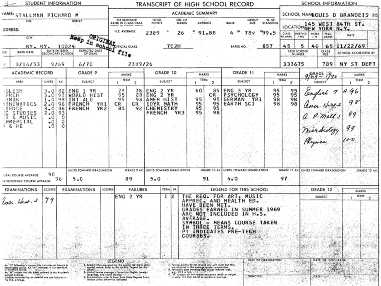
\includegraphics{transcript}
  \caption{\ifdefined\eng Stallman's senior-year transcript at Louis D. Brandeis H.S., November, 1969. Note turnaround in English class performance. ``He was forced to kowtow to a certain degree,'' says his mother, ``but he did it.''\fi\ifdefined\chs 到了1969年11月,当斯托曼即将从布兰德斯高中毕业时,他的英语成绩已经相当出色了。李普曼回忆说:``他虽然很不情愿写作文,但是他还是出色的完成了学业。''\fi}
\end{figure}
\fi

\ifdefined\eng
Outside the classroom, Stallman pursued his studies with even more diligence, rushing off to fulfill his laboratory-assistant duties at Rockefeller University during the week and dodging the Vietnam protesters on his way to Saturday school at Columbia. It was there, while the rest of the Science Honors Program students sat around discussing their college choices, that Stallman finally took a moment to participate in the preclass bull session.
\fi

\ifdefined\chs
学校以外的活动里,斯托曼表现得更加勤奋。每周他都会去洛克菲勒大学,完成实验员的工作;周六则一路避开反越战抗议者的队伍,去哥伦比亚大学参加科学之星计划的学习班。终于又有机会,科学之星计划的学生凑在一起,聊起未来将去哪所大学。
\fi

\ifdefined\eng
Recalls Breidbart, ``Most of the students were going to Harvard and MIT, of course, but you had a few going to other Ivy League schools. As the conversation circled the room, it became apparent that Richard hadn't said anything yet. I don't know who it was, but somebody got up the courage to ask him what he planned to do.''
\fi

\ifdefined\chs
布莱德巴特回忆:``绝大部分学生都会去哈佛或者麻省理工学院。当然也有人去其他几所常春藤学校。大家聊着说着,斯托曼始终没说话。这时候有个人跳出来,问斯托曼究竟去哪所大学。''
\fi

\ifdefined\eng
Thirty years later, Breidbart remembers the moment clearly. As soon as Stallman broke the news that he, too, would be attending Harvard University in the fall, an awkward silence filled the room. Almost as if on cue, the corners of Stallman's mouth slowly turned upward into a self-satisfied smile.
\fi

\ifdefined\chs
三十多年过去了,布莱德巴特依旧清晰地记得那一刻。``哈佛大学''几个字从斯托曼口中一出,人群一时没了声音。一切都好像事先排练好的一样,坐在角落中的斯托曼露出了一丝微笑。
\fi

\ifdefined\eng
Says Breidbart, ``It was his silent way of saying, `That's right. You haven't got rid of me yet.'\hspace{0.01in}''
\fi

\ifdefined\chs
布莱德巴特说:``那微笑好像在说:`没错,你们还没把我甩开呢。'\hspace{0.01in}''
\fi

\theendnotes
\setcounter{endnote}{0}

%% Copyright (c) 2002, 2010 Sam Williams
%% Copyright (c) 2010 Richard M. Stallman
%% Permission is granted to copy, distribute and/or modify this
%% document under the terms of the GNU Free Documentation License,
%% Version 1.3 or any later version published by the Free Software
%% Foundation; with no Invariant Sections, no Front-Cover Texts, and
%% no Back-Cover Texts. A copy of the license is included in the
%% file called ``gfdl.tex''.

\chapter{\ifdefined\eng
Impeach God
\fi
\ifdefined\chs
逆天行道,选举上帝
\fi}

\ifdefined\eng
Although their relationship was fraught with tension, Richard Stallman would inherit one noteworthy trait from his mother: a passion for progressive politics.
\fi

\ifdefined\chs
尽管理查德·斯托曼和母亲的关系比较紧张,但他还是继承了母亲的一个特质:对激进政治极度热情。
\fi

\ifdefined\eng
It was an inherited trait that would take several decades to emerge, however. For the first few years of his life, Stallman lived in what he now admits was a ``political vacuum.''\endnote{See Michael Gross, ``Richard Stallman: High School Misfit, Symbol of Free Software, MacArthur-certified Genius'' (1999).} Like most Americans during the Eisenhower age, the Stallman family spent the Fifties trying to recapture the normalcy lost during the wartime years of the 1940s.
\fi

\ifdefined\chs
可这个特质要在十几年之后才在斯托曼身上显现出来。他早年的生活,用他现在的话说,是与``政治绝缘''的\endnote{参见迈克尔·格劳斯的采访:《理查德·斯托曼:中学校园里的怪才,自由软件界的旗手,麦克阿瑟奖获得者》(1999年)。}。正如艾森豪威尔时期的大多数美国家庭一样,五十年代,斯托曼一家试图重拾二战以前的那份宁静、安逸的正常生活。
\fi

\ifdefined\eng
``Richard's father and I were Democrats but happy enough to leave it at that,'' says Lippman, recalling the family's years in Queens. ``We didn't get involved much in local or national politics.''
\fi

\ifdefined\chs
``理查德的父亲和我虽然都是民主党人,可我们觉得那段时间的生活还算过得去。''李普曼回忆着当年和理查德·斯托曼的父亲住在纽约市皇后区的日子,``我们当时并没有参与太多的当地或者全国的政治活动。''
\fi

\ifdefined\eng
That all began to change, however, in the late 1950s when Alice divorced Daniel Stallman. The move back to Manhattan represented more than a change of address; it represented a new, independent identity and a jarring loss of tranquility.
\fi

\ifdefined\chs
然而,五十年代末期,李普曼的离异打破了这一切。她要重新搬回纽约市曼哈顿区,这不仅仅是改个住址,它更意味着一份全新的独立生活的开始,更意味着重回喧嚣的大都市生活。
\fi

\ifdefined\eng
``I think my first taste of political activism came when I went to the Queens public library and discovered there was only a single book on divorce in the whole library,'' recalls Lippman. ``It was very controlled by the Catholic church, at least in Elmhurst, where we lived. I think that was the first inkling I had of the forces that quietly control our lives.''
\fi

\ifdefined\chs
``关于政治活动,我最初的体验是在离婚期间。当时我走进皇后区公共图书馆,却发现关于离婚的只有一本。那里当时被天主教严格控制着,至少在我们住的阿母赫斯特区是这样的。这是我第一次意识到,我们的日常生活,被周围的各种权威力量悄悄地控制着。''李普曼说。
\fi

\ifdefined\eng
Returning to her childhood neighborhood, Manhattan's Upper West Side, Lippman was shocked by the changes that had taken place since her departure to Hunter College a decade and a half before. The skyrocketing demand for post-war housing had turned the neighborhood into a political battleground. On one side stood the pro-development city-hall politicians and businessmen hoping to rebuild many of the neighborhood's blocks to accommodate the growing number of white-collar workers moving into the city. On the other side stood the poor Irish and Puerto Rican tenants who had found an affordable haven in the neighborhood.
\fi

\ifdefined\chs
重回童年居住过的纽约市曼哈顿上西城,李普曼被周围的变化震惊了。十五年前,她离家去亨特学院读书。如今,由于战后住房资源紧张,当地居民对高楼有大量需求。为了建高楼,几个街区成了一个政治决斗场。人们分成了两派:一派人,主要是政客和商人,他们希望把这一片拆迁扩建,以应付越来越多的白领移居到这里;另一派人,主要是来自爱尔兰或波多黎各的房客,他们都不富裕,所幸已经在这里找到了便宜舒适的住房。他们不想请来白领租户,因为那样会抬高当地房价和租金。
\fi

\ifdefined\eng
At first, Lippman didn't know which side to choose. As a new resident, she felt the need for new housing. As a single mother with minimal income, however, she shared the poorer tenants' concern over the growing number of development projects catering mainly to wealthy residents. Indignant, Lippman began looking for ways to combat the political machine that was attempting to turn her neighborhood into a clone of the Upper East Side.
\fi

\ifdefined\chs
一开始,李普曼不知道站到哪一边。作为一个新来的住户,她觉得的确有必要扩建。可作为一个拿着微薄收入的单亲母亲,她和那些房客有着一样的忧虑,觉得周围越来越多的项目,都是为有钱人开发的。心中忿忿不平,李普曼开始寻找机会,来和庞大的政治机器做斗争,避免让政客把上西城变成上东城那样,只供有钱人吃喝玩乐。
\fi

\ifdefined\eng
Lippman says her first visit to the local Democratic party headquarters came in 1958. Looking for a day-care center to take care of her son while she worked, she had been appalled by the conditions encountered at one of the city-owned centers that catered to low-income residents. ``All I remember is the stench of rotten milk, the dark hallways, the paucity of supplies. I had been a teacher in private nursery schools. The contrast was so great. We took one look at that room and left. That stirred me up.''
\fi

\ifdefined\chs
李普曼第一次去民主党总部是在1958年。当时,她希望为儿子找个日托所,以便在自己工作的时候,有人照顾他。在本市的低收入人员帮助中心里,她一下子被那里的环境吓到了。``我就记得当时那股酸臭的坏牛奶味儿,黑洞洞的走廊,还有那么一丁点的救助物资。我以前是护士学校的老师,是个爱干净的人。护士学校的环境和这个帮助中心的反差太大了。我们看了一眼中心里日托所的房间,就立马走人了---环境实在太让人恶心。''
\fi

\ifdefined\eng
The visit to the party headquarters proved disappointing, however. Describing it as ``the proverbial smoke-filled room,'' Lippman says she became aware for the first time that corruption within the party might actually be the reason behind the city's thinly disguised hostility toward poor residents. Instead of going back to the headquarters, Lippman decided to join up with one of the many clubs aimed at reforming the Democratic party and ousting the last vestiges of the Tammany Hall machine. Dubbed the Woodrow Wilson/FDR Reform Democratic Club, Lippman and her club began showing up at planning and city-council meetings, demanding a greater say.
\fi

\ifdefined\chs
这次造访民主党总部,让李普曼很失望。``大家说的一点也没错,乌烟瘴气,不是个干净地方。''李普曼说,这是她第一次意识到,大家之所以看不起穷人,甚至仇视他们,党内腐败也许才是一切症结所在。李普曼没有再踏入民主党总部一步。她看到当地众多俱乐部,都志在促进民主党的党内改革。李普曼加入了其中的一个俱乐部:伍德罗·威尔逊/FDR民主党改革俱乐部,从此与坦慕尼协会余党\endnote{译注:坦慕尼协会曾是纽约市民主党的政治机器。曾一度控制了曼哈顿一带民主党候选人的提名。二十世纪三十年代因操纵选票丑闻而一蹶不振。但在五十年代又有起色,六十年代左右逐渐退出政治舞台。}作斗争。李普曼开始出现在俱乐部内部的例行会议中,和市政委员会的会议上,以此她取得了更多话语权。
\fi

\ifdefined\eng
``Our primary goal was to fight Tammany Hall, Carmine DeSapio and his henchman,''\endnote{Carmine DeSapio holds the dubious distinction of being the first Italian-American boss of Tammany Hall, the New York City political machine. For more information on DeSapio and the politics of post-war New York, see John Davenport, ``Skinning the Tiger: Carmine DeSapio and the End of the Tammany Era,'' \textit{New York Affairs} (1975): 3:1.} says Lippman. ``I was the representative to the city council and was very much involved in creating a viable urban-renewal plan that went beyond simply adding more luxury housing to the neighborhood.''
\fi

\ifdefined\chs
李普曼说:``我们的主要目标,是对抗以卡米思·德·萨皮奥(Carmine De Sapio)为首的坦慕尼协会和它的追随者\endnote{卡米思·德·萨皮奥(Carmine De Sapio)曾是坦慕尼协会的第一个意大利裔主席。关于他和纽约二战后的政治格局,参见约翰·达文波特的文章《擒虎:卡米思·德·萨皮奥,和坦慕尼协会的最后时光》,《纽约事务》(1975):3:1。John Davenport, "Skinning the Tiger: Carmine DeSapio and the End of the Tammany Era," New York Affairs (1975): 3:1.}。我是市政委员会的一名代表委员。主要提议修建更多廉价住房,反对单纯修建舒适豪宅。''
\fi

\ifdefined\eng
Such involvement would blossom into greater political activity during the 1960s. By 1965, Lippman had become an ``outspoken'' supporter for political candidates like William Fitts Ryan, a Democrat elected to Congress with the help of reform clubs and one of the first U.S. representatives to speak out against the Vietnam War.
\fi

\ifdefined\chs
这种参与在六十年代变成了更大的政治活动。1965年,李普曼已经开始公开支持一些民主党的议会候选人,比如威廉·菲茨·赖安,他在各个民主党改革俱乐部的帮助下,进入议会,并成为当时第一批反对越战的议员。
\fi

\ifdefined\eng
It wasn't long before Lippman, too, was an outspoken opponent of U.S. involvement in Indochina. ``I was against the Vietnam War from the time Kennedy sent troops,'' she says. ``I had read the stories by reporters and journalists sent to cover the early stages of the conflict. I really believed their forecast that it would become a quagmire.''
\fi

\ifdefined\chs
不久之后,李普曼也开始公开反对美国涉足印度支那问题。``自从肯尼迪政府把军队送去越南,我就一直反对越战。从一开始,我就读各种来自前线的报道文章。很多文章都预测美国政府会因此深陷泥潭,我也非常赞同这个观点。''
\fi

\ifdefined\eng
Such opposition permeated the Stallman-Lippman household. In 1967, Lippman remarried. Her new husband, Maurice Lippman, a major in the Air National Guard, resigned his commission to demonstrate his opposition to the war. Lippman's stepson, Andrew Lippman, was at MIT and temporarily eligible for a student deferment. Still, the threat of induction should that deferment disappear, as it eventually did, made the risk of U.S. escalation all the more immediate. Finally, there was Richard who, though younger, faced the prospect of being drafted as the war lasted into the 1970s.
\fi

\ifdefined\chs
这种反战之声充斥在这个家庭之中。1967年,李普曼再婚。她的新任丈夫莫里斯·李普曼是一名空军少校,越战开始他辞职以示反战。莫里斯的儿子,李普曼的继子,安德鲁·李普曼当时正在麻省理工学院读书。他暂时还可以申请延期入伍。可随着战事升级,战争时间一久,入伍时间到期,他还是要去服役。当战事延续到七十年代,理查德·斯托曼虽然年纪还小,可也不得不考虑入伍的问题。他要么选择去越南参战,要么选择到加拿大避开兵役。
\fi

\ifdefined\eng
``Vietnam was a major issue in our household,'' says Lippman. ``We talked about it constantly: what would we do if the war continued, what steps Richard or his stepbrother would take if they got drafted. We were all opposed to the war and the draft. We really thought it was immoral.''
\fi

\ifdefined\chs
李普曼说:``越南问题成了家里的重点,我们总是不停地讨论它:如果战争持续下去我们怎么办?要是理查德或者安德鲁收到征兵令怎么办。我们全家都反对这征兵令,更反对这场战争。我们从心里觉得这场战争是不道德的。''
\fi

\ifdefined\eng
For Stallman, the Vietnam War elicited a complex mixture of emotions: confusion, horror, and, ultimately, a profound sense of political impotence. As a kid who could barely cope in the mild authoritarian universe of private school, Stallman experienced a shiver whenever the thought of Army boot camp presented itself. He did not think he could get through it and emerge sane.
\fi

\ifdefined\chs
对于理查德·斯托曼来说,越战给他带来的情感是复杂的:恐惧,不解,以及最终给他带来的一种政治上无能为力的感受。斯托曼如此地厌恶权威,他甚至无法忍受私立学校的威权制度。别说参军,哪怕就只让他想想军队里的训练,都会令他不寒而栗。
\fi

\ifdefined\eng
``I was devastated by the fear, but I couldn't imagine what to do and didn't have the guts to go demonstrate,'' recalls Stallman, whose March 16th birthday earned him a low number in the dreaded draft lottery.  This did not affect him immediately, since he had a college deferment, one of the last before the U.S. stopped granting them; but it would affect him in a few years. ``I couldn't envision moving to Canada or Sweden. The idea of getting up by myself and moving somewhere. How could I do that? I didn't know how to live by myself. I wasn't the kind of person who felt confident in approaching things like that.''
\fi

\ifdefined\chs
``我当时被吓坏了。可我也不知道能做什么,该怎么做。更没胆量去上街参加游行。''斯托曼如是说。1971年,政府最终取消了学生延期入伍的政策。抽签征兵\endnote{译注:抽签征兵,1969年至1975年期间,美国实行的一种征兵制度。根据生日,在适龄青年男性中,随机分配征兵顺序。顺序在前的人将最先收到征兵令。}的结果让他很是担心:他3月18日的生日,征兵顺序中比较靠前。``我很难想象要移民到加大拿或者瑞典。要一个人离开过日子,我当时可不行。我根本不知道怎么照顾自己,我对自己在生活自理方面的能力非常不自信。''
\fi

\ifdefined\eng
Stallman says he was impressed by the family members who did speak out. Recalling a sticker, printed and distributed by his father, likening the My Lai massacre to similar Nazi atrocities in World War II, he says he was ``excited'' by his father's gesture of outrage. ``I admired him for doing it,'' Stallman says. ``But I didn't imagine that I could do anything. I was afraid that the juggernaut of the draft was going to destroy me.''
\fi

\ifdefined\chs
斯托曼说,他至今依然感慨家人在公开场合的反战行为。他记得父亲车上有一个车贴,把美莱村屠杀\endnote{译注:美莱村屠杀,1968年3月16日,美军因怀疑村民掩护越共逃亡,在越南广义省美莱村展开了屠杀。}比作纳粹的大屠杀。这个车贴是父亲亲自制作的,他还做了很多这样的车贴,分发给大家。斯托曼说,他很受父亲情绪的鼓舞。``我很崇拜他这么做。''斯托曼坦言,``可我没想过自己能做什么。当时我很害怕自己的一辈子就这样被征兵令毁了。''
\fi

\ifdefined\eng
\ifdefined\vone
Although descriptions of his own unwillingness to speak out carry a tinge of nostalgic regret,
\fi
\ifdefined\vtwo
However, 
\fi
Stallman says he was turned off by the tone and direction of much of that movement. Like other members of the Science Honors Program, he saw the weekend demonstrations at Columbia as little more than a distracting spectacle.\endnote{Chess, another Columbia Science Honors Program alum, describes the protests as ``background noise.'' ``We were all political,'' he says, ``but the SHP was important. We would never have skipped it for a demonstration.''} Ultimately, Stallman says, the irrational forces driving the anti-war movement became indistinguishable from the irrational forces driving the rest of youth culture. Instead of worshiping the Beatles, girls in Stallman's age group were suddenly worshiping firebrands like Abbie Hoffman and Jerry Rubin. To a kid already struggling to comprehend his teenage peers, slogans like ``make love not war'' had a taunting quality. Stallman did not want to make war, at least not in Southeast Asia, but nobody was inviting him to make love either.
\fi

\ifdefined\chs
然而,斯托曼也逐渐开始不喜欢反战运动的方向和调调。正如其他科学之星计划的学生一样,斯托曼每周末都会看到聚集在哥伦比亚大学的抗议群众\endnote{柴斯(Chess)是哥伦比亚科学之星计划的另一个学生。他把当时的抗议游行形容为``背景噪声''。``我们都关心政治。可科学之星计划对我们来说更重要。我们从没有翘课去游行。''}。最终,斯托曼形容说,各种非理智力量把反战运动变得与各种其他青年人的非理智活动一样可怕。一瞬间,那个年级的姑娘们都不再崇拜披头士,改去崇拜各路反战领袖,如阿比·霍夫曼(Abbie
Hoffman)和杰里·鲁宾(Jerry Rubin)。理查德·斯托曼,这个中学生里的异类,面对各种流行趋势已然有些应接不暇了,如今又来了``要做爱不作战''这种花哨口号,实在让他觉得甚是沮丧。他显然不喜欢战争,至少不喜欢这次在东南亚的战争。可这也并不意味着就有会有个姑娘愿意与他一起共度春宵。
\fi

\ifdefined\eng
``I didn't like the counter culture much,'' Stallman recalls. ``I didn't like the music. I didn't like the drugs. I was scared of the drugs. I especially didn't like the anti-intellectualism, and I didn't like the prejudice against technology. After all, I loved a computer. And I didn't like the mindless anti-Americanism that I often encountered. There were people whose thinking was so simplistic that if they disapproved of the conduct of the U.S. in the Vietnam War, they had to support the North Vietnamese. They couldn't imagine a more complicated position, I guess.''
\fi

\ifdefined\chs
``我并不喜欢这种反抗文化。''斯托曼坦言,``我不喜欢他们的音乐,不喜欢毒品。我可害怕毒品。我更厌恶他们那套反理性反知识的论调,厌恶他们对各种技术的偏见。因为无论怎么说,我还是喜欢计算机的。我还经常遇到各种没头脑的反美意见,这也让我很反感。有些人的头脑真的太过简单了,他们觉得如果要反对美国参加越战,就意味着支持北越政权。他们就天真到想不出另外一种可能。''
\fi

\ifdefined\eng
Such comments underline a trait that would become the key to Stallman's own political maturation. For Stallman, political confidence was directly proportionate to personal confidence. By 1970, Stallman had become confident in few things outside the realm of math and science. Nevertheless, confidence in math gave him enough of a foundation to examine the extremes of the anti-war movement in purely logical terms.  Doing so, Stallman found the logic wanting. Although opposed to the war in Vietnam, Stallman saw no reason to disavow war as a means for defending liberty or correcting injustice.
\fi

\ifdefined\chs
这样的评论标志着斯托曼自己政治思想的逐步成熟。对于他来说,政治上的信心和自信心成正比。到了1970,斯托曼已经在数学和科学以外的一些领域里树立起了自信。当然,在数学方面的信心和能力,作为基础,让斯托曼可以从纯逻辑的角度分析越战。这种分析最终带来的结论,让斯托曼觉得,尽管反对越战,但不可否认,战争在维护自由和捍卫正义方面起到了积极作用。
\fi

\ifdefined\eng
In the 1980s, a more confident Stallman decided to make up for his past inactivity by participating in mass rallies for abortion rights in Washington DC.  ``I became dissatisfied with my earlier self for failing in my duty to protest the Vietnam War,'' he explains.
\fi

\ifdefined\chs
八十年代,斯托曼已经不再沉默。他带着这份自信,在华盛顿市参加了维护堕胎权利的聚会。``我开始不满从前的自己,觉得不该像当初那样逃避游行抗议,这是我的权利,更是我的责任。''
\fi

\ifdefined\eng
In 1970, Stallman left behind the nightly dinnertime conversations about politics and the Vietnam War as he departed for Harvard. Looking back, Stallman describes the transition from his mother's Manhattan apartment to life in a Cambridge dorm as an ``escape.'' At Harvard, he could go to his room and have peace whenever he wanted it. Peers who watched Stallman make the transition, however, saw little to suggest a liberating experience.
\fi

\ifdefined\chs
1970年,斯托曼离开了家,离开了每晚家中餐桌上的越战和政治讨论,去了哈佛大学。他回忆,从曼哈顿母亲的公寓,转到马萨诸塞州剑桥市的哈佛大学宿舍,对自己来说是一种``逃离''。可同龄人来看,他的这次大逃离并没有给他带来多少解放。
\fi

\ifdefined\eng
``He seemed pretty miserable for the first while at Harvard,'' recalls Dan Chess, a classmate in the Science Honors Program who also matriculated at Harvard. ``You could tell that human interaction was really difficult for him, and there was no way of avoiding it at Harvard. Harvard was an intensely social kind of place.''
\fi

\ifdefined\chs
``他在哈佛的第一年很痛苦。''丹·柴斯(Dan
Chess),另外一位去了哈佛大学的科学之星的学生,回忆道,``简单的人际交往对于斯托曼来说都是非常困难的。可这种交往在哈佛又是无法避免的。哈佛校园就是个大社交场。''
\fi

\ifdefined\eng
To ease the transition, Stallman fell back on his strengths: math and science. Like most members of the Science Honors Program, Stallman breezed through the qualifying exam for Math 55, the legendary ``boot camp'' class for freshman mathematics ``concentrators'' at Harvard. Within the class, members of the Science Honors Program formed a durable unit. ``We were the math mafia,'' says Chess with a laugh. ``Harvard was nothing, at least compared with the SHP.''
\fi

\ifdefined\chs
为了让这种过渡更顺畅,理查德·斯托曼重新埋头在自己的老伙伴中间:数学和自然科学。与很多科学之星计划的成员一道,斯托曼轻松通过数学55的课前考试,获得了选修数学55的资格。所谓数学55,是哈佛大学一门数学类课程的官方编号。它专门为未来数学家设计,以难度大而闻名全校。在这门课上,科学之星的成员凑成了一个小团体。``我们数学党的。''柴斯笑道:``跟科学之星比,哈佛不在话下。''
\fi

\ifdefined\eng
To earn the right to boast, however, Stallman, Chess, and the other SHP alumni had to get through Math 55. Promising four years worth of math in two semesters, the course favored only the truly devout. ``It was an amazing class,'' says David Harbater, a former ``math mafia'' member and now a professor of mathematics at the University of Pennsylvania. ``It's probably safe to say there has never been a class for beginning college students that was that intense and that advanced. The phrase I say to people just to get it across is that, among other things, by the second semester we were discussing the differential geometry of Banach manifolds. That's usually when their eyes bug out, because most people don't start talking about Banach manifolds until their second year of graduate school.''
\fi

\ifdefined\chs
可要修成正果,斯托曼,柴斯和其他科学之星成员,必须要通过数学55。这个课程把本该四年学完的数学知识,全部放在两个学期里。只有真正肯下功夫的人,才能啃下这块硬骨头。``那真是门让人神往的课。''戴维·哈伯特(David Harbater)回忆道。他曾是这门课上``数学党''的成员,如今已是宾夕法尼亚大学数学系教授。``很保守地说,几乎没有几个给大学新生设计的课程,能这么难,这么深,课业量也很少有这么大的。我经常给人这么形容这门课的难度:第二个学期,我们已经开始讲巴拿赫空间的微分几何了。一般人听了肯定瞪大眼睛,因为绝大多数人到了研究生第二年才开始说点巴拿赫空间的东西。''
\fi

\ifdefined\eng
Starting with 75 students, the class quickly melted down to 20 by the end of the second semester. Of that 20, says Harbater, ``only 10 really knew what they were doing.'' Of that 10, 8 would go on to become future mathematics professors, 1 would go on to teach physics.
\fi

\ifdefined\chs
那年这门课刚一开始有75个学生,到第二学期结束,就只有20个学生还在坚持\endnote{译注:美国大学允许学生在学期开始之前选课,上过几周,如果觉得不合适,可以放弃这门课。所以一个课程在开始的时候会有很多人上,但到了学期结束只有一部分人坚持选下了这门课,拿到成绩。}。戴维·哈伯特说,这20个学生当中,``只有10个人真正听懂了课上讲的是什么。这10个人里,8个人后来做了数学教授,另外有一个做了物理教授。''
\fi

\ifdefined\eng
``The other one,'' emphasizes Harbater, ``was Richard Stallman.''
\fi

\ifdefined\chs
``最后那一个,''戴维·哈伯特强调,``就是理查德·斯托曼。''
\fi

\ifdefined\eng
Seth Breidbart, a fellow Math 55 classmate, remembers Stallman distinguishing himself from his peers even then.
\fi

\ifdefined\chs
赛思·布莱德巴特也是数学55课上的学生,他记得当时斯托曼就显出了与众不同的特质。
\fi

\ifdefined\eng
``He was a stickler in some very strange ways,'' says Breidbart. There is a standard technique in math which everybody does wrong. It's an abuse of notation where you have to define a function for something and what you do is you define a function and then you prove that it's well defined. Except the first time he did and presented it, he defined a relation and proved that it's a function. It's the exact same proof, but he used the correct terminology, which no one else did. That's just the way he was.''
\fi

\ifdefined\chs
``遇到一些事,他总是特别能坚持。当时,我们经常用一种错误的方法来解题。每次我们要定义一个函数的时候,我们都会先定义一个函数,然后证明这个函数是良构的。这么做本身是用错了术语。斯托曼第一次也犯了这个错。可后来,他都是先定义一个关系,然后证明这个关系是一个函数。其实证明的过程都一样,但他用了正确的符号和术语。而其他没有一个人这么做。他就是这么个人。''
\fi

\ifdefined\eng
It was in Math 55 that Richard Stallman began to cultivate a reputation for brilliance. Breidbart agrees, but Chess, whose competitive streak refused to yield, says the realization that Stallman might be the best mathematician in the class didn't set in until the next year. ``It was during a class on Real Analysis,'' says Chess, now a math professor at Hunter College. ``I actually remember in a proof about complex valued measures that Richard came up with an idea that was basically a metaphor from the calculus of variations. It was the first time I ever saw somebody solve a problem in a brilliantly original way.''
\fi

\ifdefined\chs
数学55的课堂上,斯托曼又一次展现了他的聪明才智。布莱德巴特早早就承认了这一点。而柴斯好胜的个性则很难让他服输,但到了第二年,他还是不得不承认,斯托曼也许是整个课堂中最优秀的数学家。如今,柴斯已是亨特学院数学系的教授,他回忆:``在一堂实验分析的课上,斯托曼想出了一个关于复测度的证明,那个证明实际上是借鉴了变分法里的一些技巧。我是第一次看到有人能自己想出来,用这么漂亮的方法解决这个问题的。''
\fi

\ifdefined\eng
For Chess, it was a troubling moment. Like a bird flying into a clear glass window, it would take a while to realize that some levels of insight were simply off limits.
\fi

\ifdefined\chs
对于柴斯来说,这的确是个恼人的时刻。他就好像一只小鸟飞到了透明玻璃前,他要花些时间,才会不甘心地意识到,有些地方,虽然看得到,却未必是自己能力所及的。
\fi

\ifdefined\eng
``That's the thing about mathematics,'' says Chess. ``You don't have to be a first-rank mathematician to recognize first-rate mathematical talent. I could tell I was up there, but I could also tell I wasn't at the first rank. If Richard had chosen to be a mathematician, he would have been a first-rank mathematician.''\endnote{Stallman doubts this, however. ``One of the reasons I moved from math and physics to programming is that I never learned how to discover anything new in the former two.  I only learned to study what others had done.  In programming, I could do something useful every day.''}
\fi

\ifdefined\chs
``这恐怕就是数学之美吧。''柴斯说:``你不必需要成为一流的数学家,就可以欣赏数学天才的作品。我就处在这么一个尴尬的地方。我算不上一流数学家。如果斯托曼当初选择做数学家的话,他肯定会是一流的。''\endnote{斯托曼对此持怀疑态度。``我离开数学和物理界,转去搞计算机,其中一个重要原因,是我觉得在数学和物理领域很难有什么新的突破。我只能每天学习别人以前做了什么。在计算机领域,我每天都可以有些新东西。''}
\fi

\ifdefined\eng
For Stallman, success in the classroom was balanced by the same lack of success in the social arena. Even as other members of the math mafia gathered to take on the Math 55 problem sets, Stallman preferred to work alone. The same went for living arrangements. On the housing application for Harvard, Stallman clearly spelled out his preferences. ``I said I preferred an invisible, inaudible, intangible roommate,'' he says. In a rare stroke of bureaucratic foresight, Harvard's housing office accepted the request, giving Stallman a one-room single for his freshman year.
\fi

\ifdefined\chs
有得就必然有失,斯托曼在课堂上的得意,换不来社交上的成功。其他数学党的成员一般都会凑在一起讨论数学55的作业,而斯托曼则自己一个人应付作业题。住宿问题上斯托曼也坚持如此。在哈佛大学住宿申请的表格上,斯托曼清晰地说出了自己对室友的要求:``我说我希望能有个几乎看不见,听不见,摸不着的室友。''宿舍管理部门这次倒是难得如此识相,竟然接受了斯托曼的要求,在他入学的第一年,给他安排了一个单人间。
\fi

\ifdefined\eng
Breidbart, the only math-mafia member to share a dorm with Stallman that freshman year, says Stallman slowly but surely learned how to interact with other students. He recalls how other dorm mates, impressed by Stallman's logical acumen, began welcoming his input whenever an intellectual debate broke out in the dining club or dorm commons.
\fi

\ifdefined\chs
布莱德巴特是数学党成员中,唯一一个在大一期间和斯托曼同住一个宿舍楼的。他回忆,斯托曼当时的确慢慢地学着如何和别人沟通交往。他记得,当时其他几个宿舍的学生,都被斯托曼严密的逻辑分析能力感染,都喜欢跟他凑在宿舍楼的大厅或者餐厅里,谈天说地。
\fi

\ifdefined\eng
``We had the usual bull sessions about solving the world's problems or what would be the result of something,'' recalls Breidbart. ``Say somebody discovers an immortality serum. What do you do? What are the political results? If you give it to everybody, the world gets overcrowded and everybody dies. If you limit it, if you say everyone who's alive now can have it but their children can't, then you end up with an underclass of people without it. Richard was just better able than most to see the unforeseen circumstances of any decision.''
\fi

\ifdefined\chs
布莱德巴特说:``我们凑一起经常会扯上一些异想天开的事情,比如如何解决各种世界问题,或者某种东西如果成真了会怎么样。好比说,有人发明了一种长生不老药会如何。你该怎么办?这东西的政治影响会是什么?如果说每人都吃了这个药,最后谁都不会老,最后人越来越多,到头来还是会因为资源困乏,大家都得死掉。老是不会老了,但终究也会死。可如果限制发布这个药,好比你可以说,只有现在活着的人能拿到这个药,新生儿不能吃长生不老药,那最后世界上就会被分出一批下等人。斯托曼总能比大家更早看出各种决策的优劣。''
\fi

\ifdefined\eng
Stallman remembers the discussions vividly. ``I was always in favor of immortality,'' he says. ``How else would we be able to see what the world is like 200 years from now?'' Curious, he began asking various acquaintances whether they would want immortality if offered it. ``I was shocked that most people regarded immortality as a bad thing.'' Many said that death was good because there was no use living a decrepit life, and that aging was good because it got people prepared for death, without recognizing the circularity of the combination.
\fi

\ifdefined\chs
斯托曼至今还清晰地记得当时的讨论:``我总是对长生不老的话题感兴趣。我们要是能看到200年之后,世界是什么样子,那会如何?''出于好奇,斯托曼找了几个朋友,问他们愿意不愿意长生不老:``我很惊讶,不少人觉得长生不老并非什么好事情。''很多人说,死亡从某种意义上讲是个好事,因为一直活下去的话生命会显得越来越没有意义。而苍老的好处则是让人们能逐渐意识到死亡的到来。
\fi

\ifdefined\eng
Although perceived as a first-rank mathematician and first-rate informal debater, Stallman shied away from clear-cut competitive events that might have sealed his brilliant reputation. Near the end of freshman year at Harvard, Breidbart recalls how Stallman conspicuously ducked the Putnam exam, a prestigious test open to math students throughout the U.S. and Canada. In addition to giving students a chance to measure their knowledge in relation to their peers, the Putnam served as a chief recruiting tool for academic math departments. According to campus legend, the top scorer automatically qualified for a graduate fellowship at any school of his choice, including Harvard.
\fi

\ifdefined\chs
尽管众人已经公认,斯托曼会是个一流数学家,也是个非正式的辩论能手,可他自己却一直避免参加各种有明确排名或分界线的竞赛。布莱德巴特清晰地记得,斯托曼大一的时候,大家眼看着他回避参加帕特南竞赛(Putnam Competition)。帕特南竞赛是专门针对美国和加拿大数学系本科生的竞赛。参赛者借此可以知道自己的数学水平,更重要的,比赛的结果经常被各大院校当作选拔研究生和博士生的依据。按照学生中间的流言来看,如果拿到好成绩,就可以去任何一所大学读研究生或博士,而且是免学费,全额奖学金。当然,这也包括哈佛大学。
\fi

\ifdefined\eng
Like Math 55, the Putnam was a brutal test of merit. A six-hour exam in two parts, it seemed explicitly designed to separate the wheat from the chaff. Breidbart, a veteran of both the Science Honors Program and Math 55, describes it as easily the most difficult test he ever took. ``Just to give you an idea of how difficult it was,'' says Breidbart, ``the top score was a 120, and my score the first year was in the 30s. That score was still good enough to place me 101st in the country.''
\fi

\ifdefined\chs
和数学55一样,帕特南竞赛也是各残酷的竞技场。两场考试,一共六个小时。这比赛是铁了心要把学生分出三六九等。布莱德巴特,这位参加了科学之星计划,也上了数学55的学生,依然觉得这个竞赛是他参加过的最难的考试。``就跟你这么说吧,满分120,我第一年的时候分数是30几分。就这分数,我还能排上第101名。''
\fi

\ifdefined\eng
Surprised that Stallman, the best student in the class, had skipped the test, Breidbart says he and a fellow classmate cornered him in the dining common and demanded an explanation. ``He said he was afraid of not doing well,'' Breidbart recalls.
\fi

\ifdefined\chs
可让人吃惊的是,斯托曼,这位全班数学最好的学生,竟然不参加这个比赛。布莱德巴特记得当时他们听到这个消息之后,几个人把斯托曼围在墙角,让他解释为什么不参加。``他说他怕做得不好。''布莱德巴特回忆。
\fi

\ifdefined\eng
Breidbart and the friend quickly wrote down a few problems from memory and gave them to Stallman. ``He solved all of them,'' Breidbart says, ``leading me to conclude that by not doing well, he either meant coming in second or getting something wrong.''
\fi

\ifdefined\chs
一听这话,布莱德巴特和其他几个学生迅速地写下了几个帕特南竞赛得题目,扔给斯托曼,让他做。``他全都做对了。我当时就觉得,所谓`做得不好',对他来说也许就是拿个亚军,或者做错一道题。''
\fi

\ifdefined\eng
Stallman remembers the episode a bit differently. ``I remember that they did bring me the questions and it's possible that I solved one of them, but I'm pretty sure I didn't solve them all,'' he says. Nevertheless, Stallman agrees with Breidbart's recollection that fear was the primary reason for not taking the test. Despite a demonstrated willingness to point out the intellectual weaknesses of his peers and professors in the classroom, Stallman hated and feared the notion of head-to-head competition -- so why not just avoid it?
\fi

\ifdefined\chs
斯托曼对这个事情的记忆则略有出入。``我确实记得他们给我题目了,可我好像记得我就做出来一道,反正肯定没全做对。''无论如何,斯托曼承认,正如布莱德巴特说的,他当时的确是出于害怕才不参加这竞赛的。斯托曼只是在班上指出同学或者老师的错误。但他却不喜欢,甚至害怕参加任何正面竞争。结果,他就总是避开类似的比赛。
\fi

\ifdefined\eng
``It's the same reason I never liked chess,'' says Stallman. ``Whenever I'd play, I would become so consumed by the fear of making a single mistake and losing that I would start making stupid mistakes very early in the game. The fear became a self-fulfilling prophecy.''  He avoided the problem by not playing chess.
\fi

\ifdefined\chs
斯托曼说:``同样的原因,我也不喜欢下棋。每次我下棋的时候,我都害怕那种一步走错,满盘皆输的情况。而这种恐惧,最后总是成真。''于是,斯托曼也就只能靠避免下棋,来解决这个问题。
\fi

\ifdefined\eng
Whether such fears ultimately prompted Stallman to shy away from a mathematical career is a moot issue. By the end of his freshman year at Harvard, Stallman had other interests pulling him away from the field. Computer programming, a latent fascination throughout Stallman's high-school years, was becoming a full-fledged passion. Where other math students sought occasional refuge in art and history classes, Stallman sought it in the computer-science laboratory.
\fi

\ifdefined\chs
究竟是不是因为这种恐惧,才没让斯托曼成为数学家,我们不得而知。但无论如何,大一结束的时候,斯托曼已经有了新的兴趣:编程。这兴趣从斯托曼中学的时候就逐渐形成,但潜伏了很久,最终在大一后期成为了他的一个主要兴趣,让他投入了自己的全部热情。其他数学系的学生都靠选修艺术类和历史课来放松,斯托曼则跑去机房缓解压力。
\fi

\ifdefined\eng
For Stallman, the first taste of real computer programming at the IBM New York Scientific Center had triggered a desire to learn more. ``Toward the end of my first year at Harvard school, I started to have enough courage to go visit computer labs and see what they had. I'd ask them if they had extra copies of any manuals that I could read.'' Taking the manuals home, Stallman would examine the machine specifications to learn about the range of different computer designs.
\fi

\ifdefined\chs
当年第一次在IBM纽约科学中心编程的经历,诱使着斯托曼去了解更多。他说:``在哈佛学习快一年的时候,我开始跑去哈佛的几个计算机实验室,看看他们那里有什么新东西。刚到那里,我就问他们能不能给我一份使用手册。''把这些使用手册拿回家,斯托曼开始自习阅读,比较各个机器这间的差别和联系。
\fi

\ifdefined\eng
One day, near the end of his freshman year, Stallman heard about a special laboratory near MIT. The laboratory was located on the ninth floor of a building in Tech Square, the mostly-commercial office park MIT had built across the street from the campus. According to the rumors, the lab itself was dedicated to the cutting-edge science of artificial intelligence and boasted the cutting-edge machines and software to match.
\fi

\ifdefined\chs
第一年快结束的时候,斯托曼有天听说在麻省理工学院,有个特殊的实验室。那个实验室就在校区旁边的技术广场大厦九层。传说,这个实验室是专门为顶尖的人工智能研究而设立,里面各种高级计算机和软件。
\fi

\ifdefined\eng
Intrigued, Stallman decided to pay a visit.
\fi

\ifdefined\chs
斯托曼被这一切吸引住了,决定亲自前往一探究竟。
\fi

\ifdefined\eng
The trip was short, about 2 miles on foot, 10 minutes by train, but as Stallman would soon find out, MIT and Harvard can feel like opposite poles of the same planet. With its maze-like tangle of interconnected office buildings, the Institute's campus offered an aesthetic yin to Harvard's spacious colonial-village yang.  Of the two, the maze of MIT was much more Stallman's style. The same could be said for the student body, a geeky collection of ex-high school misfits known more for its predilection for pranks than its politically powerful alumni.
\fi

\ifdefined\chs
从哈佛大学到那里并不远,走路大概三公里,坐地铁只要十分钟。可等到了那里,斯托曼才发现,麻省理工学院和哈佛大学,简直就像两个世界。麻省理工学院里真可说是``五步一楼,十步一阁''。各个建筑纠缠在一起;相比之下,哈佛大学则显得明快宽敞。两所大学,一张一弛,一阴一阳。这不仅体现在建筑风格上,在校风学风上也是如此。麻省理工学院的学生,多是中学里的怪才,他们好开玩笑,喜欢恶作剧;而哈佛大学的学生,则更多是家有深厚背景的孩子,或是从小就有政治抱负的青年。
\fi

\ifdefined\eng
The yin-yang relationship extended to the AI Lab as well. Unlike Harvard computer labs, there was no grad-student gatekeeper, no clipboard waiting list for terminal access, no atmosphere of ``look but don't touch.'' Instead, Stallman found only a collection of open terminals and robotic arms, presumably the artifacts of some AI experiment. When he encountered a lab employee, he asked if the lab had any spare manuals it could loan to an inquisitive student. ``They had some, but a lot of things weren't documented,'' Stallman recalls. ``They were hackers, after all,'' he adds wryly, referring to hackers' tendency to move on to a new project without documenting the last one.
\fi

\ifdefined\chs
这种学校风格同样延伸到计算机实验室中。与哈佛的各个计算机实验室不同,麻省理工大学的这个人工智能实验室,没有门卫;没有拿着小本子,记下等候使用终端的人,给他们排队的人;也没有贴着``严禁触摸''标识的那种氛围。到了那里,斯托曼就看到了几个空着没人用的终端,和几个机械臂,提醒着人们这里正在做着人工智能方面的试验。斯托曼找到一位在这里上班的雇员,问他能不能送自己一份使用手册。斯托曼回忆:``那人说他手头确实有几份闲置的手册,可好多东西都没写在手册里。怎么说,他们也是黑客。''斯托曼笑道,暗指黑客们往往会直奔下一个项目,而不去把之前的项目记录在文档里。
\fi

\ifdefined\eng
Stallman left with something even better than a manual: A job.  His first project was to write a PDP-11 simulator that would run on a PDP-10. He came back to the AI Lab the next week, grabbing an available terminal, and began writing the code.
\fi

\ifdefined\chs
在对方的帮助下,斯托曼最终得到了一份比手册更好的东西:一个在实验室的工作职位\endnote{译注:美国学生一般会在校内或校外找些工作,一方面可以积累经验,但很重要的一方面是可以挣钱交学费。}。他的第一个工作任务,是在PDP-10上写一个PDP-11的模拟器。于是,他第二周又来到人工智能实验室,找了个终端,开始写代码。
\fi

\ifdefined\eng
Looking back, Stallman sees nothing unusual in the AI Lab's willingness to accept an unproven outsider at first glance. ``That's the way it was back then,'' he says. ``That's the way it still is now. I'll hire somebody when I meet him if I see he's good. Why wait? Stuffy people who insist on putting bureaucracy into everything really miss the point. If a person is good, he shouldn't have to go through a long, detailed hiring process; he should be sitting at a computer writing code.''
\fi

\ifdefined\chs
回想起来,斯托曼觉得,人工智能实验室把一份工作``随便''扔给一个素不相识的外校学生这件事,并没什么不妥。``当年都是这样,如今也是如此。我见一个人,他要是很优秀,我就雇他。等什么呢?很多刻板的人喜欢在每件事上都安插各种官僚流程。这实在太愚蠢。要是一个人真的很优秀,他就不会花时间准备各种冗长拖沓的面试。他应该踏踏实实坐电脑前头写代码。''
\fi

\ifdefined\eng
To get a taste of ``bureaucratic and stuffy,'' Stallman need only visit the computer labs at Harvard. There, access to the terminals was doled out according to academic rank. As an undergrad, Stallman sometimes had to wait for hours. The waiting wasn't difficult, but it was frustrating. Waiting for a public terminal, knowing all the while that a half dozen equally usable machines were sitting idle inside professors' locked offices, seemed the height of irrational waste. Although Stallman continued to pay the occasional visit to the Harvard computer labs, he preferred the more egalitarian policies of the AI Lab. ``It was a breath of fresh air,'' he says. ``At the AI Lab, people seemed more concerned about work than status.''
\fi

\ifdefined\chs
要想了解什么是``刻板''和``官僚流程'',斯托曼说只要去哈佛的计算机实验室看看就行了。在那里,使用终端的先后顺序,是按照年级排序的。作为一个本科生,斯托曼经常要等好几个小时才能用上计算机。等待本身并不是件难事,但却是个很无聊的事情。尤其是你明明知道,在各个教授的办公室里,都有一个能用的计算机终端,可每个办公室的房门都是紧锁的,你就只能在那里按部就班地等着用那几台公共终端。在斯托曼看来,这实在是暴殄天物。尽管他后来也会偶尔去哈佛大学的计算机实验室,但他显然更喜欢人工智能实验室的平等环境。他说:``在那里总算能呼吸到新鲜空气了。人工智能实验室里,人们更关心手头的工作,而不是各自的地位状态。''
\fi

\ifdefined\eng
Stallman quickly learned that the AI Lab's first-come, first-served policy owed much to the efforts of a vigilant few. Many were holdovers from the days of Project MAC, the Department of Defense-funded research program that had given birth to the first time-share operating systems. A few were already legends in the computing world. There was Richard Greenblatt, the lab's in-house Lisp expert and author of MacHack, the computer chess program that had once humbled AI critic Hubert Dreyfus. There was Gerald Sussman, original author of the robotic block-stacking program HACKER. And there was Bill Gosper, the in-house math whiz already in the midst of an 18-month hacking bender triggered by the philosophical implications of the computer game LIFE.\endnote{See Steven Levy, \textit{Hackers} (Penguin USA [paperback], 1984): 144.\\Levy devotes about five pages to describing Gosper's fascination with LIFE, a math-based software game first created by British mathematician John Conway. I heartily recommend this book as a supplement, perhaps even a prerequisite, to this one.}
\fi

\ifdefined\chs
斯托曼很快了解到,人工智能实验室这种先到先用的原则,很大一部分要归功于当年一批警觉的小团体。其中很多人,参与了当年国防部资助的MAC项目(Porject MAC)。在这个项目里,他们开发了第一个分时操作系统。而这个小团体中的有些人,如今已经在世界计算机史册上留了名。包括实验室中的Lisp专家理查德·格林布拉特(Richard Greenblatt),他设计了国际象棋程序MacHack,让休伯特·德莱弗斯(Hubert Dreyfus)关于人工智能的观点受到重创\endnote{译注:休伯特·德莱弗斯(Hubert Dreyfus),美国哲学家。曾在1965年断言,计算机下国际象棋不可能战胜一个十岁孩子。参见他的论文《Alchemy and Artificial Intelligence》};还有著名的杰拉尔德·萨斯曼(Gerald Sussman),他曾设计HACKER这个程序,利用机器人解决堆垛问题;也有著名的数学怪才比尔·高斯伯(Bill Gosper),他当年发现了生命游戏(LIFE game)中的模式并因此获奖\endnote{参见史蒂芬·李维(Steven Levy),《黑客》(1984年,美国企鹅出版社),第144页。史蒂芬用了五页来描述高斯伯如何迷恋生命游戏。生命游戏是英国数学家约翰·康威建立的数学模型。强烈建议读一下《黑客》一书,可以作为本书的补充读物。}。
\fi

\ifdefined\eng
Members of the tight-knit group called themselves ``hackers.'' Over time, they extended the ``hacker'' description to Stallman as well. In the process of doing so, they inculcated Stallman in the ethical traditions of the ``hacker ethic.'' In their fascination with exploring the limits of what they could make a computer do, hackers might sit at a terminal for 36 hours straight if fascinated with a challenge. Most importantly, they demanded access to the computer (when no one else was using it) and the most useful information about it. Hackers spoke openly about changing the world through software, and Stallman learned the instinctual hacker disdain for any obstacle that prevented a hacker from fulfilling this noble cause. Chief among these obstacles were poor software, academic bureaucracy, and selfish behavior.
\fi

\ifdefined\chs
这批小团体里的人把自己称作``黑客''。当然,在不久的将来,他们也会把斯托曼归类为``黑客''。在成为``黑客''的过程中,斯托曼被逐渐地引进黑客文化的小圈子里。这群人,会痴迷于不断挖掘计算机的极限。他们遇到挑战,可以一连36个小时坐在终端显示器前面工作。最重要的,他们对计算机和各种相关信息都有无尽的需求。他们会公开大谈如何用计算机和软件改变世界。斯托曼也逐渐学到,黑客们会本能地蔑视任何阻止他们实现这一伟大梦想的障碍和困难。这些障碍之中,最为重要的有以下几个方面:一是低劣的软件,二是各种学术官僚主义,三是自私自利的行为。
\fi

\ifdefined\eng
Stallman also learned the lore, stories of how hackers, when presented with an obstacle, had circumvented it in creative ways. This included various ways that hackers had opened professors' offices to ``liberate'' sequestered terminals. Unlike their pampered Harvard counterparts, MIT faculty members knew better than to treat the AI Lab's limited stock of terminals as private property. If a faculty member made the mistake of locking away a terminal for the night, hackers were quick to make the terminal accessible again -- and to remonstrate with the professor for having mistreated the community.  Some hackers did this by picking locks (``lock hacking''), some by removing ceiling tiles and climbing over the wall.  On the 9th floor, with its false floor for the computers' cables, some spelunked under it.  ``I was actually shown a cart with a heavy cylinder of metal on it that had been used to break down the door of one professor's office,''\endnote{Gerald Sussman, an MIT faculty member and hacker whose work at the AI Lab predates Stallman's, disputes this story. According to Sussman, the hackers never broke any doors to retrieve terminals.} Stallman says.
\fi

\ifdefined\chs
斯托曼在这里学到的东西里,还包括黑客们解决问题的各种新颖技巧和相关的轶事。这其中,就包括黑客们如何打开教授们紧锁的办公室门,``解放''被囚禁的计算机终端。哈佛大学的计算机终端每天都被娇生惯养;相比之下,麻省理工学院的教授们更了解如何应付有限的终端资源。要是哪位教授,把某个终端锁在自己的办公室里过夜,黑客们就会想法把终端重新搞到手。之后,还会大摇大摆走到教授面前,劝诫他不要如此对待实验室的同僚。黑客们的做法多种多样,有些人会直接撬锁,他们自称这是``黑''锁术;有些人则会把天花板打开,爬到天花板上面,从天花板和房顶中间的通风空隙中爬入教授的办公室;在大厦的第九层,地板和楼层地面中间有空隙,本来是用于铺设机房的电线,而黑客们则会撬开地板,从下面溜进办公室。斯托曼说:``我当初还给他们展示过一架手推车,上面放着一个实心的圆柱形金属,这东西后来就曾用来撞开办公室的门\endnote{杰拉尔德·萨斯曼(Gerald Sussman),他既是麻省理工学院的教授,也同时是人工智能实验室里的一名黑客。他在人工智能实验室工作的时候,斯托曼还没来。根据他的回忆,当时黑客们根本没有破门进入教授的办公室。}。''
\fi

\ifdefined\eng
The hackers' insistence served a useful purpose by preventing the professors from egotistically obstructing the lab's work.  The hackers did not disregard people's particular needs, but insisted that these be met in ways that didn't obstruct everyone else.  For instance, professors occasionally said they had something in their offices which had to be protected from theft.  The hackers responded, ``No one will object if you lock your office, although that's not very friendly, as long as you don't lock away the lab's terminal in it.''
\fi

\ifdefined\chs
黑客们如此坚持,使得教授们很难起私心而阻碍整个实验室的工作。当然黑客们也没有无视教授们的个人需求,只是教授的需求不能影响到别人。比如,有些教授有时候会辩解称,自己办公室里有重要的私人物品,所以必须要锁门。黑客们则会回应:``你锁上办公室的门没问题,但是别把实验室的终端也锁在里面。''
\fi

\ifdefined\eng
Although the academic people greatly outnumbered the hackers in the AI Lab, the hacker ethic prevailed. The hackers were the lab staff and students who had designed and built parts of the computers, and written nearly all the software that users used.  They kept everything working, too.  Their work was essential, and they refused to be downtrodden.  They worked on personal pet projects as well as features users had asked for, but sometimes the pet projects revolved around improving the machines and software even further. Like teenage hot-rodders, most hackers viewed tinkering with machines as its own form of entertainment.
\fi

\ifdefined\chs
虽然在人数上,黑客们处于劣势,但黑客的文化在不断追求、不断进步的计算机领域还是占了上风。这些黑客,很多是实验室的成员,或者是学生。实验室的计算机上,有些硬件就是他们设计的;而几乎所有软件,都是这些黑客写的。他们不仅创造了整个系统,还维护着这个系统的运行。他们的工作至关重要,因此他们拒绝来自任何方面的压抑。他们会根据其他用户的需求写程序,也会同时维护着自己的个人项目。有时候,这些个人项目会越来越庞大,甚至影响深远。黑客们每天为计算机系统增砖添瓦,并以此为乐。
\fi

\ifdefined\eng
Nowhere was this tinkering impulse better reflected than in the operating system that powered the lab's central PDP-10 computer. Dubbed ITS, short for the Incompatible Time Sharing system, the operating system incorporated the hacking ethic into its very design. Hackers had built it as a protest to Project MAC's original operating system, the Compatible Time Sharing System, CTSS, and named it accordingly. At the time, hackers felt the CTSS design too restrictive, limiting programmers' power to modify and improve the program's own internal architecture if needed. According to one legend passed down by hackers, the decision to build ITS had political overtones as well. Unlike CTSS, which had been designed for the IBM 7094, ITS was built specifically for the PDP-6. In letting hackers write the system themselves, AI Lab administrators guaranteed that only hackers would feel comfortable using the PDP-6. In the feudal world of academic research, the gambit worked. Although the PDP-6 was co-owned in conjunction with other departments, AI researchers soon had it to themselves.  Using ITS and the PDP-6 as a foundation, the Lab had been able to declare independence from Project MAC shortly before Stallman's arrival.\endnote{\textit{Ibid.}}
\fi

\ifdefined\chs
这种工作的结果之一,就是运行在实验室核心的PDP-10计算机上的操作系统。它被称做ITS,全称``非兼容型分时系统''(Incompatible Time Sharing system)。这个系统从头到脚都体现着黑客的文化。它的诞生,本来是用来抗议MAC项目的操作系统:CTSS,即``兼容型分时系统''(Compatible Time Sharing System)。这种抗议从名字中的``非兼容型''几个字上就能看出来。当时,黑客们觉得CTSS的很多设计太过严苛,因为它限制了程序员改进现有程序的行为。沿袭着黑客们一贯以来的作风,设计ITS的决定本身就是政治上正确的。CTSS本身是为IBM 7094设计的,ITS则是为PDP-6设计。为了让黑客们更好地写出自己的操作系统,人工智能实验室的管理员保证可以让黑客们使用PDP-6计算机。在分封制度盛行的学术圈,这策略确实奏效。虽然PDP-6以前是和其他几个系共用的,可后来最终还是归了人工智能的研究人员。斯托曼来之前的那段时间,黑客们终于利用ITS和这台PDP-6做基础,正式宣告自己独立于MAC项目\endnote{同上}。
\fi

\ifdefined\eng
By 1971, ITS had moved to the newer but compatible PDP-10, leaving the PDP-6 for special stand-alone uses. The AI PDP-10 had a very large memory for 1971, equivalent to a little over a megabyte; in the late 70s it was doubled.   Project MAC had bought two other PDP-10s; all were located on the 9th floor, and they all ran ITS.  The hardware-inclined hackers designed and built a major hardware addition for these PDP-10s, implementing paged virtual memory, a feature lacking in the standard PDP-10.\endnote{I apologize for the whirlwind summary of ITS' genesis, an operating system many hackers still regard as the epitome of the hacker ethos. For more information on the program's political significance, see Simson Garfinkel, \textit{Architects of the Information Society: Thirty-Five Years of the Laboratory for Computer Science at MIT} (MIT Press, 1999).}
\fi

\ifdefined\chs
1971年,ITS被安装在更新一代的PDP-10上。那台老的PDP-6则被单独拿出来以做他用。人工智能实验室这台PDP-10有大约1MB的内存,在当时算是非常大的了。到七十年代末,又给它的内存加了一倍。MAC项目也为实验室带来了两台PDP-10,它们都被放在大厦九楼,运行着ITS系统。PDP-10本身没有内存分页机制。为此,对硬件感兴趣的黑客们为这三台PDP-10设计了内存分页模块\endnote{原谅我草草地带过了ITS的历史。这个操作系统至今依然被很多黑客视为黑客文化的缩影。关于这个操作系统的更多历史,参见西姆森·加芬克尔(Simson Garfinkel)的书《信息社会的建筑师:麻省理工学院计算机实验室的三十五年》(麻省理工学院出版社,1999年)。Architects of the Information Society: Thirty-Five Years of the Laboratory for Computer Science at MIT}。
\fi

\ifdefined\eng
As an apprentice hacker, Stallman quickly became enamored with ITS. Although forbidding to some non-hackers, ITS boasted features most commercial operating systems wouldn't offer for years (or even to this day), features such as multitasking, applying the debugger immediately to any running program, and full-screen editing capability. 
\fi

\ifdefined\chs
作为一名黑客学徒,斯托曼一下子被ITS迷住了。尽管ITS会吓跑一些门外汉,可它却比其他商业操作系统提早几年实现了很多特性,甚至有些特性是今天很多商业操作系统都没有提供的。这包括多任务系统,在线调试任何运行中的程序,全屏编辑等等。
\fi

\ifdefined\eng
``ITS had a very elegant internal mechanism for one program to examine another,'' says Stallman, recalling the program. ``You could examine all sorts of status about another program in a very clean, well-specified way.''  This was convenient
not only for debugging, but also for programs to start, stop or control other programs.
\fi

\ifdefined\chs
斯托曼回忆:``ITS内部有一套非常优雅的机制,可以让一个程序实时监测另一个运行中的程序。你可以获得另外某个程序的各种信息,内容清晰,接口明确。''这个功能不仅对调试程序有很大帮助,而且可以轻松地开关和控制别的程序。
\fi

\ifdefined\eng
Another favorite feature would allow the one program to freeze another program's job cleanly, between instructions. In other operating systems, comparable operations might stop the program in the middle of a system call, with internal status that the user could not see and that had no well-defined meaning. In ITS, this feature made sure that monitoring the step-by-step operation of a program was reliable and consistent.
\fi

\ifdefined\chs
另外一个功能,就是允许一个程序暂停另一个程序,让那个程序停在指定的两个指令之间。在别的操作系统里,类似的功能只能让程序停留在某个系统调用中,把程序停在这个状态,会有很多内部隐藏状态用户都看不到。而在ITS里,这一功能则可以保证一条指令一条指令地监视另一个程序运行,并且能做到停顿之后,一样能继续运行。
\fi

\ifdefined\eng
``If you said, `Stop the job,' it would always be stopped in user mode. It would be stopped between two user-mode instructions, and everything about the job would be consistent for that point,'' Stallman says. ``If you said, `Resume the job,' it would continue properly. Not only that, but if you were to change the (explicitly visible) status of the job and continue it, and later change it back, everything would be consistent. There was no hidden status anywhere.''
\fi

\ifdefined\chs
斯托曼说:``如果你说:`把这个任务暂停',那它肯定会停在用户态。而且会停在两条用户态的指令中间。任何运行过程中的变量状态,都会保留。你再说:`继续跑它',它就真的会继续跑下去,不会因为暂停而搞乱程序,导致前后不一致。还不止如此,你还能把某个变量或者哪个状态给修改了。让它继续跑,然后再把它改回去,这程序就能和当初一样。所有状态都是用户可见的,没有什么隐藏状态。''
\fi

\ifdefined\eng
Starting in September 1971, hacking at the AI Lab had become a regular part of Stallman's weekly school schedule. From Sunday through Friday, Stallman was at Harvard. As soon as Friday afternoon arrived, however, he was on the subway, heading down to MIT for the weekend. Stallman usually made sure to arrive well before the ritual food run. Joining five or six other hackers in their nightly quest for Chinese food, he would jump inside a beat-up car and head across the Harvard Bridge into nearby Boston. For the next hour or so, he and his hacker colleagues would discuss everything from ITS to the internal logic of the Chinese language and pictograph system. Following dinner, the group would return to MIT and hack code until dawn, or perhaps go to Chinatown again at 3 a.m.
\fi

\ifdefined\chs
从1971年开始,斯托曼每周都会定期跑去人工智能实验室。周日到周五,斯托曼会呆在哈佛大学。一到了周五下午,他就坐上地铁,直奔麻省理工学院,在那里度过整个周末。他一般会在晚饭时间赶到,然后约上五六个黑客,一起去吃中餐。他们跳进一辆旧车上,穿过哈佛大桥,直奔波士顿。接下来的四个小时里,他们凑在一起就开始谈天说地。话题从ITS系统,一直到汉语和象形文字的内在逻辑。晚饭结束,这群人再回到麻省理工,写代码一直到天亮。期间也许会在半夜三点多的时候,再跑去唐人街一趟。
\fi

\ifdefined\eng
Stallman might stay up all morning hacking, or might sleep Saturday morning on a couch. On waking he would hack some more, have another Chinese dinner, then go back to Harvard.  Sometimes he would stay through Sunday as well.  These Chinese dinners were not only delicious; they also provided sustenance lacking in the Harvard dining halls, where on the average only one meal a day included anything he could stomach. (Breakfast did not enter the count, since he didn't like most breakfast foods and was normally asleep at that hour.)
\fi

\ifdefined\chs
第二天上午,斯托曼也许会继续折腾代码,也有可能找个沙发睡上一觉。醒来之后,他会继续写代码,找点中餐吃吃,然后回到哈佛。有时候,他会再多呆一天,等到周日再回去。这些中餐不仅美味,而且比哈佛大学食堂的菜内容丰富,营养全面。吃上一顿能管一天。所以斯托曼他们一般一天也就吃一顿饭。(对于他来说,早餐一般不在考虑范围之内。一方面,早餐中的食物他不喜欢;另一方面,早餐时间他一般都会睡大觉。)
\fi

\ifdefined\eng
For the geeky outcast who rarely associated with his high-school peers, it was a heady experience to be hanging out with people who shared the same predilection for computers, science fiction, and Chinese food. ``I remember many sunrises seen from a car coming back from Chinatown,'' Stallman would recall nostalgically, 15 years after the fact in a speech at the Swedish Royal Technical Institute. ``It was actually a very beautiful thing to see a sunrise, 'cause that's such a calm time of day. It's a wonderful time of day to get ready to go to bed. It's so nice to walk home with the light just brightening and the birds starting to chirp; you can get a real feeling of gentle satisfaction, of tranquility about the work that you have done that night.''\endnote{See Richard Stallman, ``RMS lecture at KTH (Sweden),'' (October 30, 1986), \url{http://www.gnu.org/philosophy/stallman-kth.html}.}
\fi

\ifdefined\chs
作为一个中学时期很少有社交活动的宅男,如今和这么多跟自己类似的人混在一起,确实让斯托曼甚是陶醉。他们这些人,都对计算机感兴趣,都喜欢科幻小说,喜欢吃中餐。``我记得很多次,我们从唐人街回来,在车上看日出。''十五年后,在瑞典皇家技术研究所的一次演讲上,斯托曼回想当年,一切依旧历历在目:``欣赏日出真的是个很享受的事情。那是一天之中最平静的时刻。也是一天之中上床睡觉的好时候。倘若这时候徒步走回家,伴着几缕阳光,耳畔回响着鸟鸣,再想想你整整一夜完成的工作,你会有种由内而外地舒适和满足感。''\endnote{参见理查德·斯托曼在瑞典皇家技术研究所的演讲(1986年10月30日):\url{http://www.gnu.org/philosophy/stallman-kth.html}}
\fi

\ifdefined\eng
The more Stallman hung out with the hackers, the more he adopted the hacker world view. Already committed to the notion of personal liberty, Stallman began to infuse his actions with a sense of communal duty. When others violated the communal code, Stallman was quick to speak out. Within a year of his first visit, Stallman was the one opening locked offices to recover the sequestered terminals that belonged to the lab community as a whole. In true hacker fashion, Stallman also sought to make his own personal contribution to the art. One of the most artful door-opening tricks, commonly attributed to Greenblatt, involved bending a stiff wire into several right angles and attaching a strip of tape to one end. Sliding the wire under the door, a hacker could twist and rotate the wire so that the tape touched the inside doorknob. Provided the tape stuck, a hacker could turn the doorknob by pulling the handle formed from the outside end of the wire.
\fi

\ifdefined\chs
斯托曼和这群黑客呆得越来越久,他也逐渐开始了解和接纳黑客们的世界观。曾经他坚持个人自由,如今,在这基础之上,又注入了公共责任的概念。当其他人违反了这种公共准则,斯托曼会毫不留情地当面指出。在麻省理工学院的第一年,斯托曼也曾想法打开教授办公室的门,拿回属于实验室的计算机终端。作为一个黑客,斯托曼也贡献了自己的开门技巧。以前大家一直用着一个开门的方法,据说是格林布拉特(Greenblatt)最先使用的。这个方法要求用到一条硬的电线,把这条电线折几个弯,从一盒磁带里抽出磁条,拴在弯过的电线一头,再把磁条做成一个绳套。开门的时候,先从门下的缝隙里把带磁条一头的电线躺着穿过门缝,等电线和磁条都进了门,再把电线立起来。来回晃几下电线,直到磁条做的绳套能套在门把手上。一旦套紧,黑客就可以把电线往后拉,这样,门就从里面被打开了。
\fi

\ifdefined\eng
When Stallman tried the trick, he found it hard to execute. Getting the tape to stick wasn't always easy, and twisting the wire in a way that turned the doorknob was similarly difficult. Stallman thought about another method: sliding away ceiling tiles to climb over the wall. This always worked, if there was a desk
to jump down onto, but it generally covered the hacker in itchy fiberglass.  Was there a way to correct that flaw?  Stallman considered an alternative approach. What if, instead of slipping a wire under the door, a hacker slid away two ceiling panels and reached over the wall with a wire?
\fi

\ifdefined\chs
当斯托曼自己亲自尝试这个方法的时候,他发现这法子操作起来难度不小。要让磁条套上门把手,可是个体力活。而之前要怎么把电线折出几个弯,也是有学问的。为此,斯托曼开始另寻他法:他开始的想法是把天花板上的板子移开,然后爬进天花板和房顶中间的通风空隙中。爬到办公室上方,跳到桌子上,一切就大功告成了。这法子一直都行得通,可这一路,总会沾上一身让人痒痒的玻璃纤维。斯托曼开始考虑怎么解决这个问题。他想到,如果不把电线从门下缝隙滑过去,而是从天花板上悬下去开门,会不会可以呢?
\fi

\ifdefined\eng
Stallman took it upon himself to try it out. Instead of using a wire, Stallman draped out a long U-shaped loop of magnetic tape with a short U of adhesive tape attached sticky-side-up at the base. Reaching across over the door jamb, he dangled the tape until it looped under the inside doorknob. Lifting the tape until the adhesive stuck, he then pulled on one end of the tape, thus turning the doorknob. Sure enough, the door opened. Stallman had added a new twist to the art of getting into a locked room.
\fi

\ifdefined\chs
斯托曼自己开始尝试。他并没有用电线,而是把一盒磁带里的磁条拿出来,拿着两端,向下悬成一个U形,把磁条有粘性的部分冲上。移开天花板上的两块板子,站到高处,把U形的磁条从通风道甩到房间里。磁条会从天花板上垂下去,晃悠几下,把U形磁条套在门把手上。接着把磁条往上一拉,门就顺势打开了。就这样,斯托曼又为黑客开门技巧做了贡献。
\fi

\ifdefined\eng
``Sometimes you had to kick the door after you turned the door knob,'' says Stallman, recalling a slight imperfection of the new method. ``It took a little bit of balance to pull it off while standing on a chair on a desk.''
\fi

\ifdefined\chs
``有时候,门锁打开后你还得踹两脚才能把门弄开。''斯托曼回忆起这个方法的一点瑕疵:``拉磁条的时候你得小心点,一般是站在一个椅子上,下面还要再垫个桌子。这时候保持平衡就很重要。''
\fi

\ifdefined\eng
Such activities reflected a growing willingness on Stallman's part to speak and act out in defense of political beliefs. The AI Lab's spirit of direct action had proved inspirational enough for Stallman to break out of the timid impotence of his teenage years. Opening up an office to free a terminal wasn't the same as taking part in a protest march, but it was effective in a way that most protests weren't: it solved the problem at hand.
\fi

\ifdefined\chs
这些活动从一个方面反映出斯托曼期望表达自己的政治诉求。人工智能实验室的实干精神,让斯托曼打破了中学以来的沉默。打开办公室的门和上街游行虽然不可同日而语,但从效率的角度分析,与游行比起来,它快速有效,能直接解决问题。
\fi

\ifdefined\eng
By the time of his last years at Harvard, Stallman was beginning to apply the whimsical and irreverent lessons of the AI Lab back at school.
\fi

\ifdefined\chs
在哈佛大学的最后一年,斯托曼把人工智能实验室的那套古灵精怪的行事理念用到了哈佛的校园里。
\fi

\ifdefined\eng
``Did he tell you about the snake?'' his mother asks at one point during an interview. ``He and his dorm mates put a snake up for student election. Apparently it got a considerable number of votes.''
\fi

\ifdefined\chs
``他跟你说那条蛇了吗?''他母亲在一次采访中突然问起,``他还有他宿舍那边的几个人一起,把一条蛇拿去参加了学生会选举。而且最后那条蛇还拿到不少选票。''
\fi

\ifdefined\eng
The snake was a candidate for election within Currier House, Stallman's dorm, not the campus-wide student council. Stallman does remember the snake attracting a fair number of votes, thanks in large part to the fact that both the snake and its owner both shared the same last name. ``People may have voted for it because they thought they were voting for the owner,'' Stallman says. ``Campaign posters said that the snake was `slithering for' the office. We also said it was an `at large' candidate, since it had climbed into the wall through the ventilating unit a few weeks before and nobody knew where it was.''
\fi

\ifdefined\chs
根据斯托曼的回忆,那条蛇实际是拿去参加了卡瑞尔楼的学生干部竞选。那是斯托曼住的宿舍楼,并非全校范围内的学生竞选。斯托曼的确记得当时那条蛇拿到了不少选票,但很大一个原因,是因为这条蛇的姓和它主人一样。``人们也许以为是给这条蛇的主人在投票。''斯托曼说,``我们的选举海报上写那条蛇是个很有`潜力'的候选人。因为竞选开始前几周,它刚刚`潜'到通风口里,我们好几个人极尽全``力''也没能找到它。''
\fi

\ifdefined\eng
Stallman and friends also ``nominated'' the house master's 3-year-old son. ``His platform was mandatory retirement at age seven,'' Stallman recalls. Such pranks paled in comparison to the fake-candidate pranks on the MIT campus, however. One of the most successful fake-candidate pranks was a cat named Woodstock, which actually managed to outdraw most of the human candidates in a campus-wide election. ``They never announced how many votes Woodstock got, and they treated those votes as spoiled ballots,'' Stallman recalls. ``But the large number of spoiled ballots in that election suggested that Woodstock had actually won. A couple of years later, Woodstock was suspiciously run over by a car. Nobody knows if the driver was working for the MIT administration.'' Stallman says he had nothing to do with Woodstock's candidacy, ``but I admired it.''\endnote{In an email shortly after this book went into its final edit cycle, Stallman says he drew political inspiration from the Harvard campus as well. ``In my first year of Harvard, in a Chinese History class, I read the story of the first revolt against the Qin dynasty,'' he says.  (That's the one whose cruel founder burnt all the books and was buried with the terra cotta warriors.)  ``The story is not reliable history, but it was very moving.''}
\fi

\ifdefined\chs
斯托曼和几个朋友还提名了楼管的三岁儿子。``给他选举时候提出的政治纲领,就是七岁强制退休。''不过,斯托曼的这些恶作剧与麻省理工学院里的选举恶作剧比起来,实在是小巫见大巫了。在麻省理工学院最成功的一次选举恶作剧,是提名一只名叫伍德斯托克的猫参加全校学生委员会的选举。最后这只猫得到的选票比许多候选人的选票都多。``他们最后也没有宣布伍德斯托克到底得了多少票。他们把这些选票当作了废票。可选举结果一出,大家看到了一大堆的废票,从废票的数量上看,伍德斯托克应该是可以赢得这次选举了。几年之后,伍德斯托克据说是在马路上被一辆车压死了。''斯托曼如此回忆道。他说他当年和伍德斯托克的选举没有一点关系,``可我很崇拜这事\endnote{本书最后一审期间,斯托曼发来邮件说,他从哈佛大学也得到了很多政治上的鼓舞。斯托曼说:``我大一的时候,修了中国历史这门课。读了很多关于反对秦朝暴政的故事。虽然很多故事也许没有史料依据,但依旧振奋人心。''}。''
\fi

\ifdefined\eng
At the AI Lab, Stallman's political activities had a sharper-edged tone. During the 1970s, hackers faced the constant challenge of faculty members and administrators pulling an end-run around ITS and its hacker-friendly design. ITS allowed anyone to sit down at a console and do anything at all, even order the system to shut down in five minutes. If someone ordered a shutdown with no good reason, some other user canceled it. In the mid-1970s some faculty members (usually those who had formed their attitudes elsewhere) began calling for a file security system to limit access to their data.   Other operating systems had such features, so those faculty members had become accustomed to living under security, and to the feeling that it was protecting them from something dangerous. But the AI Lab, through the insistence of Stallman and other hackers, remained a security-free zone.
\fi

\ifdefined\chs
在人工智能实验室,斯托曼的政治活动更加积极,产生的矛盾也更尖锐。在七十年代,学校的一些教授和管理员一度发出通知,说即将停止在实验室的计算机上运行ITS,也将停止支持很多黑客们喜欢的设计。ITS允许任何人坐在终端前,做任何事情。包括把整个计算机关机。这在当年,可是个大事。因为很多人都会通过终端使用同一台计算机,关机意味着其他人也必须暂停手上的工作。不过,如果别人关机,你会收到即将关机的通知。要是你手头的工作还没完成,你也可以取消这次关机操作。到了七十年代中期,一些教授开始对文件的安全保护提出要求,要求他们能够控制哪些用户才能访问自己的文件。可人工智能实验室的这些黑客们,还是坚持要维护一个没有控制的系统。
\fi

\ifdefined\eng
Stallman presented both ethical and practical arguments against adding security. On the ethical side, Stallman appealed to the AI Lab community's traditions of intellectual openness and trust. On the practical side, he pointed to the internal structure of ITS, which was built to foster hacking and cooperation rather than to keep every user under control.  Any attempt to reverse that design would require a major overhaul. To make it even more difficult, he used up the last empty field in each file's descriptor for a feature to record which user had most recently changed the file. This feature left no place to store file security information, but it was so useful that nobody could seriously propose to remove it.
\fi

\ifdefined\chs
于是,斯托曼对这些安全控制特性从道德和实践上给予了否定。从道德上说,人工智能实验室的这个圈子里,大家都有着开放和信任的传统。从实践上看,ITS系统本身也是为了开发和协作而设计的,并非要控制哪些用户。任何与这初衷相违背的特性都需要额外的精力来开发维护,完全没有必要。为了让安全特性更难实现,斯托曼把文件描述符的最后一点富裕空间,用来存储用户的最后修改时间。最后修改时间是个很重要的信息,谁也不想把它去掉。可这么一来,整个文件描述符也就没有任何地方来存储安全信息了。
\fi

\ifdefined\eng
``The hackers who wrote the Incompatible Timesharing System decided that file protection was usually used by a self-styled system manager to get power over everyone else,'' Stallman would later explain. ``They didn't want anyone to be able to get power over them that way, so they didn't implement that kind of a feature. The result was, that whenever something in the system was broken, you could always fix it'' (since access control did not stand in your way).\endnote{See Richard Stallman (1986).}
\fi

\ifdefined\chs
``设计ITS的黑客们认为,文件访问控制这个特性,是为自私的系统管理员设计的,这样他们这些管理员就可以凌驾在任何用户之上。''斯托曼事后解释:``黑客们可不希望有谁被任何人控制约束,所以他们不会实现这样的功能。这么做的结果是,一旦系统出了毛病,任何人都能赶在第一时间修复它。''(因为没有访问控制功能去阻止你去访问任何文件。)\endnote{参见上述的斯托曼在瑞典皇家技术研究所的演讲。}
\fi

\ifdefined\eng
Through such vigilance, hackers managed to keep the AI Lab's machines security-free. In one group at the nearby MIT Laboratory for Computer Sciences, however, security-minded faculty members won the day. The DM group installed its first password system in 1977. Once again, Stallman took it upon himself to correct what he saw as ethical laxity. Gaining access to the software code that controlled the password system, Stallman wrote a program to decrypt the encrypted passwords that the system recorded.  Then he started an email campaign, asking users to choose the null string as their passwords. If the user had chosen ``starfish,'' for example, the email message looked something like this:
\fi

\ifdefined\chs
这种警觉,让黑客们得以在人工智能实验室营造出一个没有管制的世界。可在旁边的麻省理工学院计算机科学实验室里,对安全敏感的教授们则取得了胜利。动态建模组最先在1977年在系统中使用了密码登陆。又一次,斯托曼挺身而出,纠正了这种自己看来``不道德''的行为。他先获得了密码登录系统代码的访问权限,然后写了一个程序,解密已经加密存储的密码。然后他开始给系统上的每个用户发邮件,劝说他们放弃使用密码。这封邮件大概是这样的:
\fi

\ifdefined\eng
\begin{quote}
I see you chose the password ``starfish''. I suggest that you switch to the password ``carriage return'', which is what I use. It's easier to type, and also opposes the idea of passwords and security.
\end{quote}
\fi

\ifdefined\chs
\begin{quote}
我看到你用``starfish''做密码了,我建议你把密码直接改成``回车'',我用的就是这个密码。这密码简单好记,而且可以让你忘了密码和安全这些繁杂琐事。
\end{quote}
\fi

\ifdefined\eng
The users who chose ``carriage return'' -- that is, users who simply pressed the Enter or Return button, entering a blank string instead of a unique password -- left their accounts accessible to the world at large, just as all accounts had been, not long before. That was the point: by refusing to lock the shiny new locks on their accounts, they ridiculed the idea of having locks. They knew that the weak security implemented on that machine would not exclude any real intruders, and that this did not matter, because there was no reason to be concerned about intruders, and that no one wanted to intrude anyway, only to visit.
\fi

\ifdefined\chs
所谓用``回车''做密码,就等同于没有密码。这个密码让其他用户也可以访问自己的帐号。这和以前没有密码的日子没什么分别。这就是斯托曼和黑客们要表达的:他们拒绝任何光鲜亮美的枷锁,他们会嘲弄任何企图使用枷锁的想法。他们知道,这种安全保护能力很弱的系统,不可能防范任何入侵者。可这无所谓,因为完全没必要考虑什么入侵者,从来就没有入侵者,只有访客。
\fi

\ifdefined\eng
Stallman, speaking in an interview for the 1984 book \textit{Hackers}, proudly noted that one-fifth of the LCS staff accepted this argument and employed the null-string password.\endnote{See Steven Levy, \textit{Hackers} (Penguin USA [paperback], 1984): 417.}
\fi

\ifdefined\chs
斯托曼在一次为1984年出版的《黑客》一书的采访中,很骄傲地提到,当年计算机科学实验室里,有五分之一的人换了``回车''做密码\endnote{参见史蒂芬·李维(Steven Levy),《黑客》(1984年,美国企鹅出版社),第417页。}。
\fi

\ifdefined\eng
Stallman's null-string campaign, and his resistance to security in general, would ultimately be defeated. By the early 1980s, even the AI Lab's machines were sporting password security systems. Even so, it represented a major milestone in terms of Stallman's personal and political maturation. Seen in the context of Stallman's later career, it represents a significant step in the development of the timid teenager, afraid to speak out even on issues of life-threatening importance, into the adult activist who would soon turn needling and cajoling into a full-time occupation.
\fi

\ifdefined\chs
斯托曼的这种反密码抗议,以及各种拒绝安全保护的行为,最终还是要失败的。八十年代起,哪怕是人工智能实验室,也开始支持密码登陆系统。可即便如此,斯托曼的行为标志着他个人政治思维成熟的里程碑。斯托曼迈出了一大步。当年他还是怯懦的中学生时,哪怕遇到决定生死的大事,他也不敢上街公开反对。如今,他则成了一个活跃人士,把各种嘻笑怒骂当作家常便饭。
\fi

\ifdefined\eng
In voicing his opposition to computer security, Stallman drew on many of the key ideas that had shaped his early life: hunger for knowledge, distaste for authority, and frustration over prejudice and secret rules that rendered some people outcasts. He would also draw on the ethical concepts that would shape his adult life: responsibility to the community, trust, and the hacker spirit of direct action. Expressed in software-computing terms, the null string represents the 1.0 version of the Richard Stallman political worldview -- incomplete in a few places but, for the most part, fully mature.
\fi

\ifdefined\chs
反对计算机安全这事,体现了斯托曼早年性格中的几个关键特质:对知识如饥似渴,对权威厌恶嘲弄;可又烦恼于别人对自己的各种偏见不解,被一些人看作异类。这些也正反映出了未来主导他行动的道德基础:对社区的责任感和信任;还有遇到问题,直接行动的黑客精神。用软件界的行话说,反密码抗议行动体现的正是斯托曼1.0版。虽然有些地方还很不完善,但大部分已经成熟。
\fi

\ifdefined\eng
Looking back, Stallman hesitates to impart too much significance to an event so early in his hacking career. ``In that early stage there were a lot of people who shared my feelings,'' he says. ``The large number of people who adopted the null string as their password was a sign that many people agreed that it was the proper thing to do. I was simply inclined to be an activist about it.''
\fi

\ifdefined\chs
斯托曼自己,则不太赞成把他这样的早年的黑客经历强调得太多。他说:``早年间,很多人都和我有同样的想法。当时那么多人最后选择了不用密码,这事实本身就说明他们很多人认为这么做是对的。我只是在这方面比较活跃。''
\fi

\ifdefined\eng
Stallman does credit the AI Lab for awakening that activist spirit, however. As a teenager, Stallman had observed political events with little idea as to how he could do or say anything of importance. As a young adult, Stallman was speaking out on matters in which he felt supremely confident, matters such as software design, responsibility to the community, and individual freedom. ``I joined this community which had a way of life which involved respecting each other's freedom,'' he says. ``It didn't take me long to figure out that that was a good thing. It took me longer to come to the conclusion that this was a moral issue.''
\fi

\ifdefined\chs
不过斯托曼依旧很感激人工智能实验室氛围唤醒了他作为政治活动家潜质。曾经还是少年的时候,斯托曼目睹了很多政治事件,他很难想象自己能做出什么有影响的事情。如今虽只过弱冠之年,他却已经可以在自己的领域里指手划脚,自信地为整个社区负责,也为个人自由出头。他说:``我加入了这个圈子,这个圈子的文化非常强调尊重每个人的自由。我很快就意识到这是个好事,可花了很长的时间后,我才觉得这是一种道德责任。''
\fi

\ifdefined\eng
Hacking at the AI Lab wasn't the only activity helping to boost Stallman's esteem. At the start of his junior year at Harvard, Stallman began participating in a recreational international folk dance group which had just been started in Currier House. He was not going to try it, considering himself incapable of dancing, but a friend pointed out, ``You don't know you can't if you haven't tried.'' To his amazement, he was good at it and enjoyed it. What started as an experiment became another passion alongside hacking and studying; also, occasionally, a way to meet women, though it didn't lead to a date during his college career.  While dancing, Stallman no longer felt like the awkward, uncoordinated 10-year-old whose attempts to play football had ended in frustration. He felt confident, agile, and alive. In the early 80s, Stallman went further and joined the MIT Folk Dance Performing Group.   Dancing for audiences, dressed in an imitation of the traditional garb of a Balkan peasant, he found being in front of an audience fun, and discovered an aptitude for being on stage which later helped him in public speaking.
\fi

\ifdefined\chs
斯托曼不仅在人工智能实验室获得了黑客们的尊重。在哈佛的第一年,斯托曼参加了一个世界民间舞蹈小组。这个小组刚刚在卡瑞尔宿舍楼成立。斯托曼一开始也没打算加入,因为他觉得自己根本不适合跳舞。可他朋友却说:``你不试试怎么知道呢?''后来他真的去试了,出乎意料的是,他不仅很擅长跳舞,而且很享受其中的乐趣。这个无心之举最后竟然发展成了他的另一大爱好。这也给了他不少机会和女孩子搭讪,可惜在大学期间,每次搭讪都没能换来单独的约会。跳舞让斯托曼明白自己不再是那个手脚不协调,不会玩橄榄球的10岁少年了。他由此变得更加自信,灵活,有活力。在八十年代早期,斯托曼走得更远了:他加入了麻省理工学院民间舞蹈表演队。他穿着巴尔干半岛的传统服饰,在观众面前表演舞蹈。这让他甚是陶醉。舞台上面对观众的经历,也为他日后在各种公共场合中演讲打下了基础。
\fi

\ifdefined\eng
Although the dancing and hacking did little to improve Stallman's social standing, they helped him overcome the sense of exclusion that had clouded his pre-Harvard life. In 1977, attending a science-fiction convention for the first time, he came across Nancy the Buttonmaker, who makes calligraphic buttons saying whatever you wish. Excited, Stallman ordered a button with the words ``Impeach God'' emblazoned on it.
\fi

\ifdefined\chs
尽管跳舞和写代码没能提高多少他的社交能力,可刚到哈佛时那种疏远不自然的感觉却从此烟消云散。1977年,在一次科幻小说聚会上,他看到了南希徽章制作机,你可以随便写点格言座右铭什么的,把它制作成徽章。斯托曼很是兴奋,他当场制作了一个徽章,上面写着``选举上帝''。
\fi

\ifdefined\eng
For Stallman, the ``Impeach God'' message worked on many levels. An atheist since early childhood, Stallman first saw it as an attempt to start a ``second front'' in the ongoing debate on religion. ``Back then everybody was arguing about whether a god existed,'' Stallman recalls. ```Impeach God' approached the subject from a completely different viewpoint. If a god was so powerful as to create the world and yet did nothing to correct the problems in it, why would we ever want to worship such a god? Wouldn't it be more just to put it on trial?''
\fi

\ifdefined\chs
在斯托曼看来,所谓``选举上帝''可以从很多层面上来解释。作为一个从小就坚持无神论的人,斯托曼把``选举上帝''看作是信仰争论的另一种角度。``那时候,很多人都在讨论上帝究竟是不是存在。`选举上帝'四个字给了人们一个全新的角度。如果说,咱们这位上帝能耐这么大,大到可以创造整个世界,可却把这个世界中的问题扔在那里,不闻不问,那我们何必要膜拜这么一个上帝呢?这样的上帝难道不该放到法庭上审讯一番吗?''
\fi

\ifdefined\eng
At the same time, ``Impeach God'' was a reference to the the Watergate scandal of the 1970s, in effect comparing a tyrannical deity to Nixon.  Watergate affected Stallman deeply. As a child, Stallman had grown up resenting authority. Now, as an adult, his mistrust had been solidified by the culture of the AI Lab hacker community. To the hackers, Watergate was merely a Shakespearean rendition of the daily power struggles that made life such a hassle for those without privilege. It was an outsized parable for what happened when people traded liberty and openness for security and convenience.
\fi

\ifdefined\chs
另一方面,``选举上帝''也影射了七十年代的水门事件。它把尼克松比作暴虐的天神。水门事件对斯托曼的影响很深。斯托曼从小就厌恶权威。如今长大成人,这份厌恶在人工智能实验室的黑客精神影响下,更加牢固。黑客们看来,水门事件好似莎士比亚剧一般,诠释着上层权力斗争如何戏虐无权的人。它恰似一幅缩影,展现着人们如何出于安全和方便的考虑,放弃自由和开放。
\fi

\ifdefined\eng
Buoyed by growing confidence, Stallman wore the button proudly. People curious enough to ask him about it received a well-prepared spiel. ``My name is Jehovah,'' Stallman would say. ``I have a secret plan to end injustice and suffering, but due to heavenly security reasons I can't tell you the workings of my plan. I see the big picture and you don't, and you know I'm good because I told you so. So put your faith in me and obey me without question. If you don't obey, that means you're evil, so I'll put you on my enemies list and throw you in a pit where the Infernal Revenue Service will audit your taxes every year for all eternity.''
\fi

\ifdefined\chs
戴上徽章,斯托曼自信满满。好奇的路人倘若问上一句,必然换来一篇准备已久的长篇大论:``我乃耶和华,从天而来,替天行道。除忧治病,铲逆为公。我眼中所见之事,并非肉眼凡胎所能看;我心中所思之物,也非莽夫俗子所能解。神谕无价,安全第一,行道之法,乃是天机,万万不可泄露。尔等世人,尽管加信于我,毋疑毋问,顺天听命。旦有不从,即为妖孽,从此名姓入簿,打入非常之所,不得入三界,列五行。妖孽之地,行严法,加重税,世代如此,不得翻案\endnote{译者注:此处翻译以意译为主。原文为:``My name is Jehovah,...I have a secret plan to end injustice and suffering, but due to heavenly security reasons I can't tell you the workings of my plan. I see the big picture and you don't, and you know I'm good because I told you so. So put your faith in me and obey me without question. If you don't obey, that means you're evil, so I'll put you on my enemies list and throw you in a pit where the Infernal Revenue Service will audit your taxes every year for all eternity.''斯托曼所说的地狱税务局(Infernal Revenue Service)和美国国家税务局(Internal Revenue Service)有同样的首字母缩写,IRS。属于常见的文字游戏。}。''
\fi

\ifdefined\eng
Those who interpreted the spiel as a parody of the Watergate hearings only got half the message. For Stallman, the other half of the message was something only his fellow hackers seemed to be hearing. One hundred years after Lord Acton warned about absolute power corrupting absolutely, Americans seemed to have forgotten the first part of Acton's truism: power, itself, corrupts. Rather than point out the numerous examples of petty corruption, Stallman felt content voicing his outrage toward an entire system that trusted power in the first place.
\fi

\ifdefined\chs
如果只是觉得这段话是对水门事件的恶搞,那只听懂了一半。另外一半,恐怕只有那群黑客的同类能听懂。百年之前,阿克頓男爵(Lord Acton)曾经发出警告:绝对权力导致绝对的腐败。而很多美国人,恐怕忘了这个警告的前半部分:权利本身导致腐败。斯托曼并没有直接列举各种腐败案例,他直指过分信任权利,从而酿成腐败的整个社会。
\fi

\ifdefined\eng
``I figured, why stop with the small fry,'' says Stallman, recalling the button and its message. ``If we went after Nixon, why not go after Mr. Big? The way I see it, any being that has power and abuses it deserves to have that power taken away.''
\fi

\ifdefined\chs
斯托曼回忆起徽章的事情,说:``我觉得,为什么把讨论就停留在这里了?如果仅仅看到水门这一桩事件,你也许只是不再信任尼克松和他的幕僚。可明天你也许就又开始信任尼克柏,尼克树,你依旧信任权力。我对待这些掌权者都是一个态度:倘若他滥用权力,就活该在哪天被剥夺权力。''
\fi

\theendnotes
\setcounter{endnote}{0}

%% Copyright (c) 2002, 2010 Sam Williams
%% Copyright (c) 2010 Richard M. Stallman
%% Copyright (c) 2014 Posts & Telecom Press
%% Permission is granted to copy, distribute and/or modify this
%% document under the terms of the GNU Free Documentation License,
%% Version 1.3 or any later version published by the Free Software
%% Foundation; with no Invariant Sections, no Front-Cover Texts, and
%% no Back-Cover Texts. A copy of the license is included in the
%% file called ``gfdl.tex''.
\chapter{\ifdefined\eng
\ifdefined\vone 
Small Puddle of Freedom
\fi
\ifdefined\vtwo
Puddle of Freedom
\fi
\fi
\ifdefined\chs
自由一隅
\fi}
\thispagestyle{empty}
\ifdefined\eng
\ifdefined\vtwo
[RMS: In this chapter, I have corrected statements about facts, including facts about my thoughts and feelings, and removed some gratuitous hostility in descriptions of events.  I have preserved Williams' statements of his own impressions, except where noted.]
\fi
\fi

\ifdefined\chs
\ifdefined\vtwo
[RMS:本章中,我纠正了第一版中的一些错误陈述。包括对我想法和感受的描写。除非标明,我都保留了威廉原文中关于他个人感受的描写。]
\fi
\fi

\ifdefined\eng
Ask anyone who's spent more than a minute in Richard Stallman's presence, and you'll get the same recollection: forget the long hair. Forget the quirky demeanor. The first thing you notice is the gaze. One look into Stallman's green eyes, and you know you're in the presence of a true believer.
\fi

\ifdefined\chs
如果谁和斯托曼在一起待上超过一分钟,感受一般都是这样:不管他那一头的长发,不管他怪异的举止,给人印象最深刻的,是斯托曼凝视你的眼神。透过他绿色的眼睛,你能看到一种真实的信仰。
\fi

\ifdefined\eng
To call the Stallman gaze intense is an understatement. Stallman's eyes don't just look at you; they look through you. Even when your own eyes momentarily shift away out of simple primate politeness, Stallman's eyes remain locked-in, sizzling away at the side of your head like twin photon beams.
\fi

\ifdefined\chs
要说斯托曼眼神犀利,都要算是轻描淡写了。他不止是看着你,他简直就是要看透看穿你的心。哪怕你出于礼貌,暂时把自己的视线从他身上移开,你依旧能感受到他的眼神像灯塔一样,锁定在你的身上。
\fi

\ifdefined\eng
Maybe that's why most writers, when describing Stallman, tend to go for the religious angle. In a 1998 \textit{Salon.com} article titled ``The Saint of Free Software,'' Andrew Leonard describes Stallman's green eyes as ``radiating the power of an Old Testament prophet.''\endnote{See Andrew Leonard, ``The Saint of Free Software,'' \textit{Salon.com} (August 1998), \url{http://www.salon.com/21st/feature/1998/08/cov_31feature.html}.} A 1999 \textit{Wired} magazine article describes the Stallman beard as ``Rasputin-like,''\endnote{See Leander Kahney, ``Linux's Forgotten Man,'' \textit{Wired News} (March 5, 1999), \url{http://www.wired.com/news/print/0,1294,18291,00.html}.} while a \textit{London Guardian} profile describes the Stallman smile as the smile of ``a disciple seeing Jesus.''\endnote{See ``Programmer on moral high ground; Free software is a moral issue for Richard Stallman believes in freedom and free software,''\textit{London Guardian} (November 6, 1999).\ifdefined\vtwo , \url{http://www.guardian.co.uk/uk/1999/nov/06/andrewbrown}.\fi

These are just a small sampling of the religious comparisons. To date, the most extreme comparison has to go to Linus Torvalds, who, in his autobiography -- see Linus Torvalds and David Diamond, \textit{Just For Fun: The Story of an \ifdefined\vone Accidentaly \fi\ifdefined\vtwo Accidental \fi Revolutionary} (HarperCollins Publishers, Inc., 2001): 58 -- writes, ``Richard Stallman is the God of Free Software.''

Honorable mention goes to Larry Lessig, who, in a footnote description of Stallman in his book -- see Larry Lessig, \textit{The Future of Ideas} (Random House, 2001): 270 -- likens Stallman to Moses:

\begin{quote}
\ldots as with Moses, it was another leader, Linus Torvalds, who finally carried the movement into the promised land by facilitating the development of the final part of the OS puzzle. Like Moses, too, Stallman is both respected and reviled by allies within the movement. He is [an] unforgiving, and hence for many inspiring, leader of a critically important aspect of modern culture. I have deep respect for the principle and commitment of this extraordinary individual, though I also have great respect for those who are courageous enough to question his thinking and then sustain his wrath.
\end{quote}

In a final interview with Stallman, I asked him his thoughts about the religious comparisons. ``Some people do compare me with an Old Testament \ifdefined\vone prophent\fi\ifdefined\vtwo prophet\fi , and the reason is Old Testament prophets said certain social practices were wrong. They wouldn't compromise on moral issues. They couldn't be bought off, and they were usually treated with contempt.''}
\fi

\ifdefined\chs
%% Patch Pending
也许这就是为什么,很多描写斯托曼的文章都会从信仰的角度开始写起\endnote{参见安德鲁⋅伦纳德的文章《\textit{自由软件圣徒}》,1998年8月:\url{http://www.salon.com/21st/feature/1998/08/cov_31feature.html}。另见《\textit{有操守的程序员;坚持自由,坚持自由软件的理查德⋅斯托曼}》,《\textit{伦敦卫报}》,1999年11月6日;\url{http://www.guardian.co.uk/uk/1999/nov/06/andrewbrown}。把斯托曼比作宗教信徒的文章还有很多。Linux的作者林纳斯⋅托瓦兹曾用更极端的语言把斯托曼比作宗教信徒。参见他2001年发表的自传《\textit{乐者为王:一场无意间发起的革命}》(\textit{Just For Fun: The Story of an Accidentaly Revolutionary},Harper Collins Publishers, Inc., 2001),第58页。托瓦兹说:``斯托曼简直就是自由软件之神。''}。但是,这些报道都忽视了斯托曼人格中脆弱的一面。盯着斯托曼的眼睛再久些,就会发现其中潜在的改变。一开始,是一种强势带着几分催眠般的眼神;可再看几次,就会发现那眼神其实是在寻求沟通,建立联系。正像斯托曼本人所怀疑的那样,如果他的个性中真的有着一些自闭症的成分,那么他的这种眼神倒确实符合这种个性。哪怕当他目光如炬地盯着一个人的时候,那个人依旧能够感受到他眼神中透出的几分迷茫和疏远。恰似受伤的猛兽一般,眼中传出几分绝望。
%%也许这就是为什么,很多描写斯托曼的文章,都会从信仰的角度开始写起。在1998年salon.com上的一篇文章,标题定为《自由软件圣徒》。作者安德鲁·伦纳德(Andrew Leonard)描述斯托曼那双绿色眼睛的时候,写道:``[它们] 散发出一种旧约中先知般的力量\endnote{参见安德鲁·伦纳德的文章《自由软件圣徒》,1998年8月:\url{http://www.salon.com/21st/feature/1998/08/cov_31feature.html}}。''1999年《\textit{连线}》杂志的一篇文章中,形容斯托曼的络腮长胡须好似拉斯普京\endnote{译注:拉希普京,全名葛列格里·叶菲莫维奇·拉斯普京。沙俄末期的一名颇受争议的东正教教徒。当时的沙皇尼古拉二世和皇后亚历山德拉笃信神秘主义,拉希普京便因此得宠。后被尤苏波夫亲王、狄密翠大公、普利希克维奇议员等人合谋刺杀。}的胡须一般\endnote{参见利安得·克尼(Leander Kahney)的文章《被Linux遗忘的人》,《连线》,1999年3月5日: http://www.wired.com/science/discoveries/news/1999/03/18291}。《伦敦卫报》则把斯托曼的微笑说成好似``门徒看到耶稣''一般\endnote{参见《有操守的程序员;坚持自由,坚持自由软件的理查德·斯托曼》,《伦敦卫报》,1999年11月6日;\url{http://www.guardian.co.uk/uk/1999/nov/06/andrewbrown}。把斯托曼比作宗教信徒的文章还有很多。Linux的作者林纳斯·托瓦兹(Linus Torvalds)曾用更极端的语言把斯托曼比作宗教信徒。参见他2001年发表的自传《好玩而已:一场无意间发起的革命》(Just For Fun: The Story of an \ifdefined\vone Accidentaly \fi\ifdefined\vtwo Accidental \fi Revolutionary,HarperCollins Publishers, Inc., 2001),第58页。托瓦兹说:``斯托曼简直就是自由软件之神。''

%%劳伦斯·雷席格(Lawrence Lessig,昵称Larry Lessig)则把它形容得有点恐怖。雷席格所著的《The Future of Ideas》一书中,第270页脚注中曾将斯托曼比作摩西:

%%\begin{quote}
%%\ldots 同摩西一样,他也是得了贵人相助:当年斯托曼开发的操作系统只差最后一个重要组件,那就是操作系统的内核。是林纳斯·托瓦兹(Linus Torvalds)开发了Linux这个自由的操作系统内核,最终将斯托曼的运动带入了当年承诺的那片``应许之地''。斯托曼也和摩西一样,在自由软件社区里,既受人尊重,也常被人指责。他为人棱角分明,也正因如此,很能激人上进。他是现代文化中不可或缺的一位领袖。斯托曼是一位卓著的人,他坚持原则和自己的信念,为此我甚是尊敬。我同样尊敬那些敢于与他共事,甚至敢于批判他想法,又能忍受他乖戾脾气的人。
%%\end{quote}

%%在本书采访的结尾,我曾问过斯托曼,想听听他对于这种将自己与宗教挂钩的说辞有什么想法。斯托曼说:``的确有些人把我和《旧约》里的先知坐对比。因为《旧约》里面一些先知把很多社会活动都预测错了。他们也不会在道德原则问题上做妥协,不会被人收买,还常常被人轻视''
%%}。
\fi

\ifdefined\eng
Such analogies serve a purpose, but they ultimately fall short. That's because they fail to take into account the vulnerable side of the Stallman persona. Watch the Stallman gaze for an extended period of time, and you will begin to notice a subtle change. What appears at first to be an attempt to intimidate or hypnotize reveals itself upon second and third viewing as a frustrated attempt to build and maintain contact. \ifdefined\vone If, as Stallman himself has suspected from time to time, his personality is the product of autism or Asperger Syndrome, his eyes certainly confirm the diagnosis. Even at their most high-beam level of intensity, they have a tendency to grow cloudy and distant, like the eyes of a wounded animal preparing to give up the ghost.\fi\ifdefined\vtwo If his personality has a touch or ``shadow'' of autism or Asperger's Syndrome, a possibility that Stallman has entertained from time to time, his eyes certainly confirm the diagnosis. Even at their most high-beam level of intensity, they have a tendency to grow cloudy and distant, like the eyes of a wounded animal preparing to give up the ghost.\fi
\fi

\ifdefined\chs
\ifdefined\spv
这些比喻有一定道理,但似乎也有不足。它们都忽视了斯托曼人格中脆弱的一面。盯着斯托曼的眼睛再久些,你会发现其中潜在的改变。一开始,是一种强势带着几分催眠般的眼神;可再看几次,就会发现那眼神其实是在寻求沟通,建立联系。\ifdefined\vone 正像斯托曼本人所怀疑的那样,\fi如果他个性中真的有着一些自闭症的成分,那么他的这种眼神倒确实符合这种个性。哪怕当他目光如炬地盯着你的时候,你依旧能够感受到他眼神中透出的几分迷茫和疏远。恰似受伤的猛兽一般,眼中传出的有几分绝望。
\fi
\fi

\ifdefined\eng
My own first encounter with the legendary Stallman gaze dates back to the March, 1999, LinuxWorld Convention and Expo in San Jose, California. Billed as a ``coming out party'' for the \ifdefined\vtwo ``\fi Linux\ifdefined\vtwo ''\fi software community, the convention also stands out as the event that reintroduced Stallman to the technology media. Determined to push for his proper share of credit, Stallman used the event to instruct spectators and reporters alike on the history of the GNU Project and the project's overt political objectives.
\fi

\ifdefined\chs
我第一次见识到传说中的斯托曼的目光,是在1999年3月的第一届LinuxWorld大会上。大会在加利福尼亚州的圣何塞市举行,是一场``Linux''社区的大聚会。其中一个环节,就是在媒体面前介绍斯托曼。斯托曼决心在这次见面会上简要回顾GNU工程的历史以及这个工程政治上的目标,以此说明自己在社区中的工作和价值。
\fi

\ifdefined\eng
As a reporter sent to cover the event, I received my own Stallman tutorial during a press conference announcing the release of GNOME 1.0, a free software graphic user interface. Unwittingly, I push an entire bank of hot buttons when I throw out my very first question to Stallman himself: \ifdefined\vone do\fi\ifdefined\vtwo ``Do\fi you think GNOME's maturity will affect the commercial popularity of the Linux operating system?\ifdefined\vtwo ''\fi
\fi

\ifdefined\chs
作为一个报道此次大会的记者,我在GNOME 1.0的媒体发布会上被斯托曼亲自上了一课。当时,我的第一个问题在无意之中触碰到了敏感话题:``请问您觉得随着GNOME逐渐成熟,是否会推进Linux的商业应用?''
\fi

\ifdefined\eng
``I ask that you please stop calling the operating system Linux,'' Stallman responds, eyes immediately zeroing in on mine. ``The Linux kernel is just a small part of the operating system. Many of the software programs that make up the operating system you call Linux were not developed by Linus Torvalds at all. They were created by GNU Project volunteers, putting in their own personal time so that users might have a free operating system like the one we have today. To not acknowledge the contribution of those programmers is both impolite and a misrepresentation of history. That's why I ask that when you refer to the operating system, please call it by its proper name, GNU/Linux.''
\fi

\ifdefined\chs
``请你不要再把整个操作系统都叫作Linux,''斯托曼回应,眼光迅速聚焦到我的身上,``Linux是一个操作系统的内核,它仅仅是操作系统的一小部分。你所说的Linux,实际还包含了很多软件。这些软件并不都是林纳斯⋅托瓦兹开发的。它们是由GNU工程的志愿者开发的,这些志愿者用自己的业余时间创造了这些软件,让用户最终可以自由使用这个操作系统。如果不提及这些开发人员的工作,那么既不礼貌,也不尊重历史。所以我坚持把这个操作系统称作GNU/Linux,也希望你这么称呼它。''
\fi

\ifdefined\eng
Taking the words down in my reporter's notebook, I notice an eerie silence in the crowded room. When I finally look up, I find Stallman's unblinking eyes waiting for me. Timidly, a second reporter throws out a question, making sure to use the term ``GNU/Linux'' instead of Linux. Miguel de Icaza, leader of the GNOME project, fields the question. It isn't until halfway through de Icaza's answer, however, that Stallman's eyes finally unlock from mine. As soon as they do, a mild shiver rolls down my back. When Stallman starts lecturing another reporter over a perceived error in diction, I feel a guilty tinge of relief. At least he isn't looking at me, I tell myself.
\fi

\ifdefined\chs
我把这段话记在采访本上,整个会场异常地安静。等到我抬起头来,才看到斯托曼的眼睛眨都不眨地盯着我,让我心生一丝胆怯。这时候,直到另外一名记者正确地使用了GNU/Linux的名字提问,才打破僵局。GNOME项目的组长,米格尔⋅德⋅伊卡萨(Miguel de Icaza)回答了这名记者的问题。伊卡萨回答到一半,斯托曼才把目光从我身上移开。这时,我才觉得些许放松。等到斯托曼继续纠正了另外一个记者的措辞问题后,我才有种罪孽被洗清的感觉。他起码不再盯着我了——我对自己说。
\fi

\ifdefined\eng
For Stallman, such face-to-face moments would serve their purpose. By the end of the first LinuxWorld show, most reporters know better than to use the term ``Linux'' in his presence, and Wired.com is running a story comparing Stallman to a pre-Stalinist revolutionary erased from the history books by hackers and entrepreneurs eager to downplay the GNU Project's overly political objectives.\ifdefined\vtwo\endnote{See Leander Kahney (1999).}\fi  Other articles follow, and while few reporters call the operating system GNU/Linux in print, most are quick to credit Stallman for launching the drive to build a free software operating system 15 years before.
\fi

\ifdefined\chs
从斯托曼的角度看,这种面对面的时刻是有意义的。这次大会结束的时候,各路记者在斯托曼面前已经改用GNU/Linux这个名字。而《连线》的记者则开始忙着写一篇通讯。这篇通讯中,斯托曼被形容为被黑客和各大公司遗忘的英雄。甚至整个GNU工程也被忽略,因为这些黑客和公司不喜欢GNU工程中的政治目标\ifdefined\vtwo\endnote{参见利安得·克尼的文章《被Linux遗忘的人》(Linux's Forgotten Man),《连线》,1999年3月5日: \url{http://www.wired.com/science/discoveries/news/1999/03/18291}}\fi 。其他类似的报道也相继出现,尽管没有在报道中使用GNU/Linux的名字,但它们大多都提及了斯托曼的贡献,说到他十五年前发起的开发自由操作系统的项目。
\fi

\ifdefined\eng
I won't meet Stallman again for another 17 months. During the interim, Stallman will revisit Silicon Valley once more for the August, 1999 LinuxWorld show. Although not invited to speak, Stallman does \ifdefined\vone managed\fi\ifdefined\vtwo manage\fi to deliver the event's best line. Accepting the show's Linus Torvalds Award for Community Service -- an award named after Linux creator Linus Torvalds -- on behalf of the Free Software Foundation, Stallman wisecracks, ``Giving the Linus Torvalds Award to the Free Software Foundation is a bit like giving the Han Solo Award to the Rebel Alliance.''
\fi

\ifdefined\chs
再次见到斯托曼,是在17个月后。在这17个月中间,斯托曼又一次前往位于硅谷的圣何塞,参加1999年8月的第二届LinuxWorld大会。尽管没有演讲,但斯托曼此次还是有目的的。他代表自由软件基金会,领取了林纳斯⋅托瓦兹社区贡献奖。斯托曼接受奖杯的时候,打趣道:``这次代表自由软件基金会领取林纳斯⋅托瓦兹社区贡献奖,感觉就像唐僧代表师徒四人去领取悟空奖\endnote{译注:原句为``Giving the Linus Torvalds Award to the Free Software Foundation is a bit like giving the Han Solo Award to the Rebel Alliance.''里面借用了《星球大战》中的人物关系。为了读者方便理解,翻译时做了意译。}。''
\fi

\ifdefined\eng
This time around, however, the comments fail to make much of a media dent. Midway through the week, Red Hat, Inc., a prominent GNU/Linux vendor, goes public. The news merely confirms what many reporters such as myself already suspect: ``Linux'' has become a Wall Street buzzword, much like ``e-commerce'' and ``dot-com'' before it. With the stock market approaching the Y2K rollover like a hyperbola approaching its vertical asymptote, all talk of free software or open source as a political phenomenon falls by the wayside.
\fi

\ifdefined\chs
可惜,这次的玩笑并没有吸引多少媒体的关注。倒是这周的红帽公司(Red Hat, Inc.)上市,引起了各路记者的关注。这是一家以发布GNU/Linux发行版为主的软件公司\endnote{译注:如今,红帽公司的业务已经逐渐扩大,并不仅仅以发布发行版为主。但依然以GNU/Linux的各种解决方案为核心。}。这次上市,印证了大多数记者的猜测:``Linux''一词,会和``电子商务''、``点com''等一样,成为华尔街上的流行语。股票市场的热闹会把大家搞得像中了千年虫病毒一般——忘掉过去,丢掉历史,把自由软件或开源的政治方面抛诸脑后。
\fi

\ifdefined\eng
Maybe that's why, when LinuxWorld follows up its first two shows with a third LinuxWorld show in August, 2000, Stallman is conspicuously absent.
\fi

\ifdefined\chs
也许这就是为什么,在2000年第三届LinuxWorld大会上,大家再也没看到斯托曼的身影。
\fi

\ifdefined\eng
My second encounter with Stallman and his trademark gaze comes shortly after that third LinuxWorld show. Hearing that Stallman is going to be in Silicon Valley, I set up a lunch interview in Palo Alto, California. The meeting place seems ironic, not only because of \ifdefined\vone the recent no-show \fi\ifdefined\vtwo his absence from the show \fi but also because of the overall backdrop. Outside of Redmond, Washington, few cities offer a more direct testament to the economic value of proprietary software. Curious to see how Stallman, a man who has spent the better part of his life railing against our culture's predilection toward greed and selfishness, is coping in a city where even garage-sized bungalows run in the half-million-dollar price range, I make the drive down from Oakland.
\fi

\ifdefined\chs
我第二次再和斯托曼见面,是在第三届LinuxWorld大会之后不久。当时我听说斯托曼又要来硅谷,我就和他联系好,定在加利福尼亚州帕罗奥多市(Palo Alto)进行采访。这个地点选得很有意思。不仅仅是因为他上次缺席LinuxWorld大会,还因为这里作为硅谷重镇,是除了微软所在的华盛顿州雷蒙德市以外,最支持专有软件经济模型的几个城市之一。而斯托曼则花费了自己整个青春和大半生的时间,去与我们文化之中的自私与贪婪作斗争。我很好奇,他来到这座城市,看着车库大小的平房里,都在做着几十万美元的买卖的现实,斯托曼会作何反应。带着好奇心,我离开奥克兰市,驱车前往帕罗奥多。
\fi

\ifdefined\eng
I follow the directions Stallman has given me, until I reach the headquarters of Art.net, a nonprofit ``virtual artists collective.'' Located in a hedge-shrouded house in the northern corner of the city, the Art.net headquarters are refreshingly run-down. Suddenly, the idea of Stallman lurking in the heart of Silicon Valley doesn't seem so strange after all.
\fi

\ifdefined\chs
按照斯托曼给我的地址,我来到了Art.net的总部。这是一家汇集各路``网上艺术家''的非营利组织。位于城市北部,坐落在一所被篱笆围起来的房子里。房子有些旧,但又透着些小清新。这氛围顿时又让我觉得,斯托曼混在硅谷,似乎也不是个很怪的想法。
\fi

\ifdefined\eng
I find Stallman sitting in a darkened room, tapping away on his gray laptop computer. He looks up as soon as I enter the room, giving me a full blast of his 200-watt gaze. When he offers a soothing ``Hello,'' I offer a return greeting. Before the words come out, however, his eyes have already shifted back to the laptop screen.
\fi

\ifdefined\chs
我看到斯托曼坐在一个背阴的房间里,正在他那台灰色笔记本电脑上敲着键盘。我一进门,他就看着我,投来了那著名的目光。互相寒暄后,他又把目光聚焦回笔记本的屏幕上。
\fi

\ifdefined\eng
``I'm just finishing an article on the spirit of hacking,'' Stallman says, fingers still tapping. ``Take a look.''
\fi

\ifdefined\chs
``我刚刚写了一篇关于黑客精神的文章,''斯托曼一边打字,一边说,``过来看看?''
\fi

\ifdefined\eng
I take a look. The room is dimly lit, and the text appears as greenish-white letters on a black background, a reversal of the color scheme used by most desktop word-processing programs, so it takes my eyes a moment to adjust. When they do, I find myself reading Stallman's account of a recent meal at a Korean restaurant. Before the meal, Stallman makes an interesting discovery: the person setting the table has left six chopsticks instead of the usual two in front of Stallman's place setting. Where most restaurant goers would have ignored the redundant pairs, Stallman takes it as challenge: find a way to use all six chopsticks at once. Like many software hacks, the successful solution is both clever and silly at the same time. Hence Stallman's decision to use it as an illustration.
\fi

\ifdefined\chs
我走过去开始读文章。房间阴暗,屏幕上编辑软件的界面,又被斯托曼设置成了黑底绿字。我读了几个字,眼睛才逐渐适应。文章开始回忆了斯托曼有次去一家韩国餐馆的经历。当时服务员摆桌的时候,在斯托曼面前放了三双筷子。一般人恐怕都会把多余的两双筷子拿开。可斯托曼却又借此开始玩起把戏,他企图找个法子,用上所有的筷子。和很多黑客技巧一样,最终的解决方案既聪明灵巧,可又傻里傻气。斯托曼以这个事情来作为整个文章的引子。
\fi

\ifdefined\eng
As I read the story, I feel Stallman watching me intently. I look over to notice a proud but child-like half smile on his face. When I praise the essay, my comment barely merits a raised eyebrow.
\fi

\ifdefined\chs
我读的时候,感觉斯托曼一直在盯着我。起身看了他一眼,见他一脸骄傲的表情,好似孩子般笑着站在那里。我夸奖了一下他的文章,勉强让他的眉毛抬了抬。
\fi

\ifdefined\eng
``I'll be ready to go in a moment,'' he says.
\fi

\ifdefined\chs
``稍等一下,我们马上就出发。''他说。
\fi

\ifdefined\eng
Stallman goes back to tapping away at his laptop. The laptop is gray and boxy, not like the sleek, modern laptops that seemed to be a programmer favorite at the recent LinuxWorld show. Above the keyboard rides a smaller, lighter keyboard, a testament to Stallman's aging hands. During the \ifdefined\vone late 1980s, when Stallman was putting in 70- and 80-hour work weeks writing the first free software tools and programs for the GNU Project, the\fi\ifdefined\vtwo mid 1990s, the\fi pain in Stallman's hands became so unbearable that he had to hire a typist. Today, Stallman relies on a keyboard whose keys require less pressure than a typical computer keyboard.
\fi

\ifdefined\chs
斯托曼坐回座位,开始继续敲键盘。他用的笔记本是个灰色的四方盒子,和LinuxWorld上看到的大多笔记本不同,斯托曼的这台没那么光鲜亮丽,也不是什么新款式。笔记本的键盘之上,还放着一个更小、更轻的键盘。斯托曼的一双大手,则在这个小键盘上飞舞。\ifdefined\vone 80年代后期,斯托曼每周都工作70~80小时,编写GNU工程中最基础的那些自由软件,\fi\ifdefined\vtwo 九十年代中期,斯托曼\fi 双手的剧痛让他无法容忍,以至于他曾一度雇用了一位打字员。今天,他用的键盘,是一种特殊的,比常规键盘按键力度更小的键盘。
\fi

\ifdefined\eng
Stallman has a tendency to block out all external stimuli while working. Watching his eyes lock onto the screen and his fingers dance, one quickly gets the sense of two old friends locked in deep conversation.
\fi

\ifdefined\chs
斯托曼在工作时,会全然不顾外界刺激。看着他眼睛盯着屏幕,手指飞舞,让人觉得斯托曼和电脑,恰似老友重逢,当下正促膝长谈。
\fi

\ifdefined\eng
The session ends with a few loud keystrokes and the slow disassembly of the laptop.
\fi

\ifdefined\chs
斯托曼用力敲了几下键盘,合上笔记本电脑,拔掉电源,结束了写作。
\fi

\ifdefined\eng
``Ready for lunch?'' Stallman asks.
\fi

\ifdefined\chs
``吃午饭去吧?''斯托曼问。
\fi

\ifdefined\eng
We walk to my car. Pleading a sore ankle, Stallman limps along slowly. Stallman blames the injury on a tendon in his left foot. The injury is three years old and has gotten so bad that Stallman, a huge fan of folk dancing, has been forced to give up all dancing activities. ``I love folk dancing \ifdefined\vone inherently\fi\ifdefined\vtwo intensely\fi ,'' Stallman laments. ``Not being able to dance has been a tragedy for me.''
\fi

\ifdefined\chs
斯托曼抱怨着自己脚踝的伤,和我一起徐步走到我的车前。他左脚跟腱三年前受了伤,让他这么一个民族舞爱好者从此告别任何舞蹈活动。斯托曼叹道:``我可喜欢跳舞了,不能跳舞对我来说简直是个悲剧。''
\fi

\ifdefined\eng
Stallman's body bears witness to the tragedy. Lack of exercise has left Stallman with swollen cheeks and a pot belly that was much less visible the year before. You can tell the weight gain has been dramatic, because when Stallman walks, he arches his back like a pregnant woman trying to accommodate an unfamiliar load.
\fi

\ifdefined\chs
这悲剧从斯托曼的身材上就体现出来了。由于缺乏锻炼,斯托曼开始发福。他的脸颊越来越圆,啤酒肚也凸出来了。你能明显看出,他的发胖简直就是一瞬间完成的。他自己都还来不及适应,以至于在走路的时候,都要撑着腰,好似一个孕妇一般。
\fi

\ifdefined\eng
\ifdefined\vone
The walk is further slowed by Stallman's willingness to stop and smell the roses, literally. Spotting a particularly beautiful blossom, he tickles the innermost petals with his prodigious nose, takes a deep sniff and steps back with a contented sigh.
\fi
\ifdefined\vtwo
The walk is further slowed by Stallman's willingness to stop and smell the roses, literally. Spotting a particularly beautiful blossom, he strokes the innermost petals against his nose, takes a deep sniff, and steps back with a contented sigh.
\fi
\fi

\ifdefined\chs
走到中途,斯托曼停下脚步,在一簇玫瑰花前俯下身子。剥开花瓣,斯托曼把鼻子凑到花蕊前,深吸一口气,然后起身长叹,甚是满足。
\fi

\ifdefined\eng
``Mmm, rhinophytophilia,''\ifdefined\vone\endnote{At the time, I thought Stallman was referring to the flower's scientific name. Months later, I would learn that \textit{rhinophytophilia} was in fact a humorous reference to the activity, i.e., Stallman sticking his nose into a flower and enjoying the moment. For another humorous Stallman flower incident, visit: \url{http://www.stallman.org/texas.html}.}\fi  he says, rubbing his back.\ifdefined\vtwo\endnote{At the time, I thought Stallman was referring to the flower's scientific name. Months later, I would learn that \textit{rhinophytophilia} was in fact a humorous reference to the activity -- i.e., Stallman's sticking his nose into a flower and enjoying the moment -- presenting it as the kinky practice of nasal sex with plants. For another humorous Stallman flower incident, visit: \url{http://www.stallman.org/articles/texas.html}.}\fi
\fi

\ifdefined\chs
``嗯,rhinophytophilia。''他揉揉腰说\endnote{开始,我还以为斯托曼说的是这花的学名。几个月后,我才发现斯托曼所谓的rhinophytophilia,原来也是他的一个玩笑。他实际是把嗅花的行为比作用鼻子和花在亲热。更多斯托曼关于花的玩笑,参见:\url{http://www.stallman.org/texas.html}。译注:rhinophytophilia是斯托曼自创的一个希腊词汇。rhino意为``鼻子'';phyto意为``花'';philia意为``爱''。}。
%%``嗯,rhinophytophilia。''\ifdefined\vone\endnote{开始,我还以为斯托曼说的是这花的学名。几个月后,我才发现斯托曼所谓的rhinophytophilia,原来也是他的一个玩笑。他实际是把嗅花的行为比作用鼻子和花做爱。更多斯托曼关于花的玩笑,参见:\url{http://www.stallman.org/texas.html}。译注:rhinophytophilia是斯托曼自创的一个希腊词汇。rhino意为``鼻子'';phyto意为``花'';philia意为``爱''。}\fi他揉揉腰说。\ifdefined\vtwo\endnote{开始,我还以为斯托曼说的是这花的学名。几个月后,我才发现斯托曼所谓的rhinophytophilia,原来也是他的一个玩笑。他实际是把嗅花的行为比作用鼻子和花做爱。更多斯托曼关于花的玩笑,参见:\url{http://www.stallman.org/articles/texas.html}。译注:rhinophytophilia是斯托曼自创的一个希腊词汇。rhino意为``鼻子'';phyto意为``花'';philia意为``爱''。}\fi
\fi

\ifdefined\eng
The drive to the restaurant takes less than three minutes. Upon recommendation from Tim Ney, former executive director of the Free Software Foundation, I have let Stallman choose the restaurant. While some reporters zero in on Stallman's monk-like lifestyle, the truth is, Stallman is a committed epicure when it comes to food. One of the fringe benefits of being a traveling missionary for the free software cause is the ability to sample delicious food from around the world. ``Visit almost any major city in the world, and chances are Richard knows the best restaurant in town,'' says Ney. ``Richard also takes great pride in knowing what's on the menu and ordering for the entire \ifdefined\vone table.''\fi\ifdefined\vtwo the table.''  (If they are willing, that is.)\fi
\fi

\ifdefined\chs
开车到餐馆不到三分钟。根据前自由软件基金会执行总监蒂姆⋅内伊(Tim Ney)的建议,我让斯托曼选择去哪家餐馆。尽管很多报道把斯托曼描述成苦行僧一般,可事实上,斯托曼在饮食方面可谓是个美食家。作为一位布道全球的自由软件使者,一个额外收获就是可以尝遍各地美食。内伊介绍:``他去了几乎全世界所有的主要城市,这让他总能知道全城最好的餐馆在哪。斯托曼知道菜单上每个菜都是什么,点上一桌美食,他经常以此为荣。''
\fi

\ifdefined\eng
For today's meal, Stallman has chosen a Cantonese-style dim sum restaurant two blocks off University Avenue, Palo Alto's main drag. The choice is partially inspired by Stallman's recent visit to China, including \ifdefined\vone a lecture stop in Guangdong province, \fi\ifdefined\vtwo a stop in Hong Kong, \fi in addition to Stallman's personal aversion to spicier Hunanese and Szechuan cuisine. ``I'm not a big fan of spicy,'' Stallman admits.
\fi

\ifdefined\chs
今天,斯托曼选择了一家广式点心店。这家店和帕罗奥多市的主干道学院街(University Ave.)相隔两个街区。选这里,一部分是因为斯托曼刚刚去过中国,期间在香港做了短暂停留,这才想当下吃点中餐。斯托曼本人并不喜欢太辣的东西,所以他也就没选川菜和湘菜。``我对辣的东西不感冒。''斯托曼坦言。
\fi

\ifdefined\eng
We arrive a few minutes after 11 a.m. and find ourselves already subject to a 20-minute wait. Given the hacker aversion to lost time, I hold my breath momentarily, fearing an outburst. Stallman, contrary to expectations, takes the news in stride.
\fi

\ifdefined\chs
快十一点的时候,我们赶到餐馆。结果发现餐馆的门前居然已经排起了长队,我们要等二十分钟才能入席。我深知黑客们不喜欢浪费时间,于是屏住呼吸,生怕斯托曼大动肝火。可出乎意料,斯托曼竟然坦然地接受了这个事实。
\fi

\ifdefined\eng
``It's too bad we couldn't have found somebody else to join us,'' he tells me. ``It's always more fun to eat with a group of people.''
\fi

\ifdefined\chs
斯托曼对我说:``就只有我们俩来了,真可惜。人多了吃起来才热闹。''
\fi

\ifdefined\eng
During the wait, Stallman practices a few dance steps. His moves are tentative but skilled. We discuss current events. Stallman says his only regret about not attending LinuxWorld was missing out on a press conference announcing the launch of the GNOME Foundation. Backed by Sun Microsystems and IBM, the foundation is in many ways a vindication for Stallman, who has long championed that free software and free-market economics need not be mutually exclusive. Nevertheless, Stallman remains dissatisfied by the message that came out.
\fi

\ifdefined\chs
等待期间,斯托曼开始走起舞步。他步步小心,可还是能看出他有点儿功底。我们开始聊起时事。斯托曼说,这次缺席LinuxWorld大会,最遗憾的部分是没能出席GNOME基金会的成立发布会。这个基金会是Sun公司和IBM一手操办,它很好地诠释了斯托曼的观点:所谓自由软件,并不与自由市场和自由经济相冲突。然而,斯托曼依旧不满意大会的论调。
\fi

\ifdefined\eng
``The way it was presented, the companies were talking about Linux with no mention of the GNU Project at all,'' Stallman says.
\fi

\ifdefined\chs
``发布的时候,各个公司都在说着Linux,闭口不提GNU工程。''斯托曼说。
\fi

\ifdefined\eng
Such disappointments merely contrast the warm response coming from overseas, especially Asia, Stallman notes. A quick glance at the Stallman 2000 travel itinerary bespeaks the growing popularity of the free software message. Between recent visits to India, China, and Brazil, Stallman has spent 12 of the last 115 days on United States soil. His travels have given him an opportunity to see how the free software concept translates into different languages of cultures.
\fi

\ifdefined\chs
这种冷漠恰恰和地球另一边的热闹形成对比。尤其是亚洲各国,甚是热情。看看斯托曼2000年的行程安排,就能看出自由软件的迅猛增长。在115天之中,斯托曼只在美国停留了12天,其他时间则在印度、中国或巴西境内。他的旅行,让他见识了自由软件如何被翻译成不同的语言,进入各国的文化。
\fi

\ifdefined\eng
``In India many people are interested in free software, because they see it as a way to build their computing infrastructure without spending a lot of money,'' Stallman says. ``In China, the concept has been much slower to catch on. Comparing free software to free speech is harder to do when you don't have any free speech. Still, the level of interest in free software during my last visit was profound.''
\fi

\ifdefined\chs
``在印度,很多人对自由软件感兴趣。因为他们觉得这样可以用很低的成本,建设起自己的计算机基础设施,''斯托曼说,``在中国,自由软件的概念就传播得相对慢了一些。我们经常把软件自由和言论自由并提,表示这是软件用户的一种基本自由,\ifdefined\nov 但听众都不太理解\fi\ifdefined\spv 可在中国,这种类比显然不太奏效:人们压根就没有过言论自由,自然也不拿自由这东西当回事了\fi 。不过无论如何,我这次的中国之行还是在一定程度上提高了自由软件的关注度。''
\fi

\ifdefined\eng
The conversation shifts to Napster, the San Mateo, California software company, which has become something of a media cause célèbre in recent months. The company markets a controversial software tool that lets music fans browse and copy the music files of other music fans. Thanks to the magnifying powers of the Internet, this so-called ``peer-to-peer'' program has evolved into a de facto online jukebox, giving ordinary music fans a way to listen to MP3 music files over the computer without paying a royalty or fee, much to record companies' chagrin.
\fi

\ifdefined\chs
话题很快转到Napster,这是一家加利福尼亚州圣马特奥市的软件公司。这几个月,这家公司成了各大媒体的宠儿。这家公司开发了一款备受争议的软件,使得音乐爱好者之间可以互相复制音乐文件。借着互联网的东风,这类称作P2P(即端到端)的软件逐渐流行。如今,Napster俨然成了大型音乐盒,让各路音乐爱好者可以免费欣赏音乐。这一下子就惹恼了各大唱片公司。
\fi

\ifdefined\eng
Although based on proprietary software, the Napster system draws inspiration from the long-held Stallman contention that once a work enters the digital realm -- in other words, once making a copy is less a matter of duplicating sounds or duplicating atoms and more a matter of duplicating information -- the natural human impulse to share a work becomes harder to restrict. Rather than impose additional restrictions, Napster execs have decided to take advantage of the impulse. Giving music listeners a central place to trade music files, the company has gambled on its ability to steer the resulting user traffic toward other commercial opportunities.
\fi

\ifdefined\chs
尽管Napster是个专有软件,但它的流行却印证了斯托曼的想法:一旦某个作品进入数字世界,或者说,一旦复制这个作品变得便宜简单,那么,分享行为作为人类的一种本能,就很难被阻止。Napster给了用户一片分享音乐的空间,这家公司接着就可以借助用户量来寻求更多商业机会。
\fi

\ifdefined\eng
The sudden success of the Napster model has put the fear in traditional record companies, with good reason. Just days before my Palo Alto meeting with Stallman, U.S. District Court Judge Marilyn Patel granted a request filed by the Recording Industry Association of America for an injunction against the file-sharing service. The injunction was subsequently suspended by the U.S. Ninth District Court of Appeals, but by early 2001, the Court of Appeals, too, would find the San Mateo-based company in breach of copyright law,\endnote{See Cecily Barnes and Scott Ard, ``Court Grants Stay of Napster Injunction,'' \textit{News.com} (July 28, 2000), \url{http://news.cnet.com/news/0-1005-200-2376465.html}.} a decision RIAA spokesperson Hillary Rosen would later proclaim \ifdefined\vone proclaim \fi a ``clear victory for the creative content community and the legitimate online marketplace.''\endnote{See ``A Clear Victory for Recording Industry in Napster Case,'' RIAA press release (February 12, 2001), \url{http://www.riaa.com/PR_story.cfm?id=372}.}
\fi

\ifdefined\chs
Napster的迅猛成功让各大唱片公司开始担心。我来帕罗奥多之前的几天,玛莉莲⋅帕特尔(Marilyn Patel)法官刚刚在美国地方法院通过了一项由美国唱片协会提交的禁令。该禁令禁止了文件共享服务。而Napster之后上诉到上诉法院,使得这个禁令被美国第九巡回上诉法院暂停。但在2001年年初,上诉法院判定Napster的确违反了版权法\endnote{参见\textit{News.com}2000年7月28日Cecily Barnes与Scott Ard所著的文章\textit{Court Grants Stay of Napster Injunction}。 \url{http://news.cnet.com/2100-1023-243817.html}}。美国唱片协会发言人希拉里⋅罗森(Hillary Rosen)对这个判决的评价是:``保护了创作者,完善了在线市场方面的法律\endnote{参见美国唱片协会于2001年2月13日发表的新闻稿Clear Victory for Recording Industry in Napster Case。\url{http://www.riaa.com/print.php?id=EA742466-C6DB-1D28-CF94-411172C649C7}。}。''
\fi

\ifdefined\eng
For hackers such as Stallman, the Napster business model is \ifdefined\vone scary\fi\ifdefined\vtwo troublesome\fi in different ways. The company's eagerness to appropriate time-worn hacker principles such as file sharing and communal information ownership, while at the same time selling a service based on proprietary software, sends a distressing mixed message. As a person who already has a hard enough time getting his own carefully articulated message into the media stream, Stallman is understandably reticent when it comes to speaking out about the company. Still, Stallman does admit to learning a thing or two from the social side of the Napster phenomenon.
\fi

\ifdefined\chs
对于斯托曼这样的黑客来说,Napster的商业模型内包含着复杂的信息。一方面,这家公司大力倡导黑客社区所欣赏的信息共享精神;而另一方面,该公司又出售着基于专有软件的服务。这种复杂性,让斯托曼对这一事件少言寡语,因为他知道,自己已经花了很大工夫去传播自己的思想,而对这种部分和自己思想相同,但很大程度上又有矛盾的事件发表评论,很容易被媒体断章取义、平添混乱。可斯托曼依旧承认,从Napster事件上,他也认识到了一些有价值的东西。
\fi

\ifdefined\eng
``Before Napster, I thought it might be \ifdefined\vone OK \fi\ifdefined\vtwo [sufficient] \fi for people to privately redistribute works of entertainment,'' Stallman says. ``The number of people who find Napster useful, however, tells me that the right to redistribute copies not only on a neighbor-to-neighbor basis, but to the public at large, is essential and therefore may not be taken away.''
\fi

\ifdefined\chs
``以前,我觉得人们私下分享娱乐信息就\ifdefined\vone 可以 \fi\ifdefined\vtwo [足够]\fi 了,''斯托曼说,``可如此庞大数量的用户在Napster上分享音乐,这让我觉得,不仅仅是私下朋友和朋友之间的共享很重要,在公共场合,公开给大家分享信息的自由也同样重要,不可剥夺。''
\fi

\ifdefined\eng
No sooner does Stallman say this than the door to the restaurant swings open and we are invited back inside by the host. Within a few seconds, we are seated in a side corner of the restaurant next to a large mirrored wall.
\fi

\ifdefined\chs
话到此,餐厅服务员赶来,告诉我们有了空位。于是我们被领班带到桌前,坐在餐厅一角,身旁的墙壁是一整面镜子。
\fi

\ifdefined\eng
The restaurant's menu doubles as an order form, and Stallman is quickly checking off boxes before the host has even brought water to the table. ``Deep-fried shrimp roll wrapped in bean-curd skin,'' Stallman reads. ``Bean-curd skin. It offers such an interesting texture. I think we should get it.''
\fi

\ifdefined\chs
服务员拿来菜单和笔,让我们在菜单上勾选要点的菜。还没等服务员把茶水拿上桌,斯托曼就已经开始在自己的菜单上点菜了。``香煎鲜虾腐皮卷,''斯托曼读着菜单,``我喜欢腐皮的口感,点一个。''
\fi

\ifdefined\eng
This comment leads to an impromptu discussion of Chinese food and Stallman's recent visit to China. ``The food in China is utterly exquisite,'' Stallman says, his voice gaining an edge of emotion for the first time this morning. ``So many different things that I've never seen in the U.S., local things made from local mushrooms and local vegetables. It got to the point where I started keeping a journal just to keep track of every wonderful meal.''
\fi

\ifdefined\chs
这一下子又引来了斯托曼关于中餐和这次访问中国的即兴评论。``中国的饮食真是博大精深,''斯托曼大声说,这要算是他整个上午嗓门最大的一次了,``各种我在美国都没听说过的食物。还有很多当地特产、当地美食。当时我又突然想起来,我要办份杂志,专门记录每顿大餐的菜谱。''
\fi

\ifdefined\eng
The conversation segues into a discussion of Korean cuisine. During the same June, 2000, Asian tour, Stallman paid a visit to South Korea. His arrival ignited a mini-firestorm in the local media thanks to a Korean software conference attended by Microsoft founder and chairman Bill Gates that same week. Next to getting his photo above Gates's photo on the front page of the top Seoul newspaper, Stallman says the best thing about the trip was the food. ``I had a bowl of naeng myun, which is cold noodles,'' says Stallman. ``These were a very interesting feeling noodle. Most places don't use quite the same kind of noodles for your naeng myun, so I can say with complete certainty that this was the most exquisite naeng myun I ever had.''
\fi

\ifdefined\chs
这讨论接着又转向韩国菜。同样也是在2000年6月,斯托曼的亚洲之行中也去了韩国。他的到来,在当地媒体引起了一个不小的轰动。这其中原因或许还要部分归功于当时也在韩国的微软创始人比尔⋅盖茨(Bill Gates)。斯托曼的照片这次上了首尔的热销报纸的头版,比尔⋅盖茨的照片竟然被挤到了下面。除了这件事情让斯托曼非常满意之外,当地的美食也让他欢欣鼓舞。他回忆道:``我吃了一碗冷面。那面条口感非常独特,我们这边都不用那种面条做冷面。我敢肯定,那冷面是我有生以来吃到的最正点的冷面。''
\fi

\ifdefined\eng
The term ``exquisite'' is high praise coming from Stallman. I know this, because a few moments after listening to Stallman rhapsodize about naeng myun, I feel his laser-beam eyes singeing the top of my right shoulder.
\fi

\ifdefined\chs
``正点''一词在斯托曼嘴里应该是很高的评价了。因为正当斯托曼介绍完冷面,我突然觉察到他的眼神飘到了我的右后方。
\fi

\ifdefined\eng
``There is the most exquisite woman sitting just behind you,'' Stallman says.
\fi

\ifdefined\chs
``你后面坐了个很正点的妹子。''斯托曼说。
\fi

\ifdefined\eng
I turn to look, catching a glimpse of a woman's back. The woman is young, somewhere in her mid-20s, and is wearing a white \ifdefined\vone sequinned\fi\ifdefined\vtwo sequined\fi dress. She and her male lunch companion are in the final stages of paying the check. When both get up from the table to leave the restaurant, I can tell without looking, because Stallman's eyes suddenly dim in intensity.
\fi

\ifdefined\chs
我赶紧回头,瞟到了一个女人的背影。这女人很年轻,二十来岁的样子。穿了一件白色裙子,裙子上贴着闪闪发亮的饰品。她和同桌的一位男性已经用完餐,正在结账。当两人起身离开的时候,我发现了斯托曼眼中瞬间失落的神情。
\fi

\ifdefined\eng
``Oh, no,'' he says. ``They're gone. And to think, I'll probably never even get to see her again.''
\fi

\ifdefined\chs
``啊!别啊!他们要走了。我估计以后也见不到她了。''斯托曼抱怨道。
\fi

\ifdefined\eng
After a brief sigh, Stallman recovers. The moment gives me a chance to discuss Stallman's reputation vis-à-vis the fairer sex. The reputation is a bit contradictory at times. A number of hackers report Stallman's predilection for greeting females with a kiss on the back of the hand.\endnote{\ifdefined\vone See Mae Ling Mak, ``Mae Ling's Story'' (December 17, 1998). \url{http://www.crackmonkey.org/pipermail/crackmonkey/1998q4/003006.htm} \fi\ifdefined\vtwo See Mae Ling Mak, ``A Mae Ling Story'' (December 17, 1998), \url{http://crackmonkey.org/pipermai l/crackmonkey/1998-December/001777.html}.\fi
So far, Mak is the only person I've found willing to speak on the record in regard to this practice, although I've heard this from a few other female sources. Mak, despite expressing initial revulsion at it, later managed to put aside her misgivings and dance with Stallman at a 1999 LinuxWorld show. \ifdefined\vone \url{http://www.linux.com/interact/potd.phtml?potd_id=44}\fi} A May 26, 2000 \textit{Salon.com} article, meanwhile, portrays Stallman as a bit of a hacker lothario. Documenting the free software-free love connection, reporter Annalee Newitz presents Stallman as rejecting traditional family values, telling her, ``I believe in love, but not monogamy.''\endnote{See Annalee Newitz, ``If Code is Free Why Not Me?'', \textit{Salon.com} (May 26, 2000), \url{http://www.salon.com/tech/feature/2000/05/26/free_love/print.html}.}
\fi

\ifdefined\chs
一声叹息,斯托曼心神回位。这倒给了我一个机会,问问斯托曼的感情生活和审美偏好。因为坊间传言,他可是个轻佻的公子。有些时候,很多传言还有些自相矛盾。很多黑客都声称,斯托曼和女性见面,都会以吻手背的方式来打招呼\endnote{\ifdefined\vone 参见Mae Ling Mak于1998年12月17日发表的\textit{Mae Ling's Story}。\url{http://www.crackmonkey.org/pipermail/crackmonkey/1998q4/003006.htm}。\fi\ifdefined\vtwo 参见Mae Ling Mak于1998年12月17日发表的《A Mae Ling Story》。\url{http://www.crackmonkey.org/pipermail/crackmonkey/1998-December/001777.html}。\fi Mak是目前为止唯一一个愿意和我聊这事,并且公开姓名的人。除了她以外,还有几个女性跟我提到过斯托曼的这种行为。Mak一开始对于斯托曼的行为比较反感。不过在1999年的LinuxWorld上,Mak也抛弃了这种偏见,还和斯托曼一起跳了段舞。\ifdefined\vone \url{http://www.linux.com/interact/potd.phtml?potd_id=44}。\fi}。在Salon.com上,有一份2000年5月26日的采访,把斯托曼描写成了一位黑客界的花花公子。文中把自由软件和自由恋爱做类比\ifdefined\spv ,作者安娜利·奈唯姿(Annalee Newitz)把斯托曼说成是拒绝传统家庭观念的叛逆者,他还说:``我相信爱情,但不相信一夫一妻\fi\endnote{参见Annalee Newitz于2000年5月26日在\textit{Salon.com}上发表的文章If Code is Free Why Not Me?。\url{http://www.salon.com/2000/05/26/free_love/}。}。\ifdefined\spv ''\fi
\fi

\ifdefined\eng
Stallman lets his menu drop a little when I bring this up. ``Well, most men seem to want sex and seem to have a rather contemptuous attitude towards women,'' he says. ``Even women they're involved with. I can't understand it at all.''
\fi

\ifdefined\chs
\ifdefined\spv
当我问起这方面问题时,斯托曼把菜单放下后说:``这个⋯⋯很多男人似乎都会不自觉地蔑视女性,看到女性就想到上床一类的事情。就连很多女人也自觉不自觉地融入到男性的这种倾向的思维中,可我无法理解这种态度。''
\fi
\fi

\ifdefined\eng
\ifdefined\vone
I mention a passage from the 1999 book Open Sources in which Stallman confesses to wanting to name the ill-fated GNU kernel after a girlfriend at the time. The girlfriend's name was Alix, a name that fit perfectly with the Unix developer convention of putting an ``x'' at the end of any new kernel name-e.g., ``Linux.'' Because the woman was a Unix system administrator, Stallman says it would have been an even more touching tribute. Unfortunately, Stallman notes, the kernel project's eventual main developer renamed the kernel HURD.\endnote{See Richard Stallman, ``The GNU Operating System and the Free Software Movement,'' Open Sources (O'Reilly \& Associates, Inc., 1999): 65.} Although Stallman and the girlfriend later broke up, the story triggers an automatic question: for all the media imagery depicting him as a wild-eyed fanatic, is Richard Stallman really just a hopeless romantic, a wandering Quixote tilting at corporate windmills in an effort to impress some as-yet-unidentified Dulcinea?
\fi
\ifdefined\vtwo
I mention a passage from the 1999 book \textit{Open Sources} in which Stallman confesses to wanting to name the GNU kernel after a girlfriend at the time. The girlfriend's name was Alix, a name that fit perfectly with the Unix developer convention of putting an ``x'' at the end names of operating systems and kernels -- e.g., ``Linux.'' Alix was a Unix system administrator, and had suggested to her friends, ``Someone should name a kernel after me.'' So Stallman decided to name the GNU kernel ``Alix'' as a surprise for her. The kernel's main developer renamed the kernel ``Hurd,'' but retained the name ``Alix'' for part of it.  One of Alix's friends noticed this part in a source snapshot and told her, and she was touched.  A later redesign of the Hurd eliminated that part.\endnote{See Richard Stallman, ``The GNU Operating System and the Free Software Movement,'' \textit{Open Sources} (O'Reilly \& Associates, Inc., 1999): 65. [RMS: Williams interpreted this vignette as suggesting that I am a hopeless romantic, and that my efforts were meant to impress some as-yet-unidentified woman.  No MIT hacker would believe this, since we learned quite young that most women wouldn't notice us, let alone love us, for our programming.  We programmed because it was fascinating.  Meanwhile, these events were only possible because I had a thoroughly identified girlfriend at the time.  If I was a romantic, at the time I was neither a hopeless romantic nor a hopeful romantic, but rather temporarily a successful one.

On the strength of that naive interpretation, Williams went on to compare me to Don Quijote.

For completeness' sake, here's a somewhat inarticulate quote from the first edition: ``I wasn't really trying to be romantic. It was more of a teasing thing. I mean, it was romantic, but it was also teasing, you know? It would have been a delightful surprise.'']}
\fi
\fi

\ifdefined\chs
\ifdefined\vone
我提到,在1999年,一本名为《开源软件文集:开源革命之声》的书中,斯托曼在一篇文章里提到,当初他想以女朋友的名字来命名GNU操作系统的内核。这位女孩子名叫Alix,因为是以x结尾,所以和Unix界对操作系统内核的命名传统非常契合,比如``Linux''就遵照了这个命名传统。Alix当初是个Unix系统管理员,所以斯托曼这么做对她来说更是一个惊喜。不过,最后内核的主要开发人员还是把内核名字改成了Hurd\endnote{参考理查德⋅斯托曼,《\textit{GNU操作系统与自由软件运动}》,《\textit{开源软件文集}》,(O'Reilly \& Associates, Inc., 1999),第65页。}。虽然最后斯托曼与她分手了,这个故事还是给我们留下了一个问题:虽然大部分的媒体上都把斯托曼描写成是一个狂热的激进分子,但斯托曼真的就是一个堂吉诃德式的古怪人物吗?他是否只知道去挑战风车,把这看成是一种浪漫,并以此来吸引他理想中的爱人?
\fi
\ifdefined\vtwo
我提到,在1999年,一本名为《开源软件文集:开源革命之声》的书中,斯托曼在一篇文章里提到,当初他想以女朋友的名字来命名GNU操作系统的内核。这位女孩子名叫Alix,因为是以x结尾,所以和Unix界对操作系统内核的命名传统非常契合,比如Linux就遵照了这个命名传统。Alix当初是个Unix系统管理员,而且曾经和她朋友开玩笑地提到过:``应该有个内核以我的名字命名。''斯托曼于是决定把GNU的内核命名为Alix,以此给她一份惊喜。可最后内核的主要开发人员把内核名字改成了Hurd,把Alix作为其中一个模块的名字。Alix的一个朋友看到源码中出现了Alix的名字,于是把这件事情告诉了她。Alix听后非常感动。之后Hurd又经历了几次重新设计,最终还是去除了Alix这个模块\endnote{参见理查德·斯托曼在《开源软件文集:开源革命之声》一书中的文章《GNU操作系统和自由软件运动》。《开源软件文集:开源革命之声》一书已由中国电力出版社于2000年出版,洪峰等人翻译。}。
\fi
\fi

\ifdefined\vtwo
\ifdefined\eng
``I wasn't really trying to be romantic,'' Stallman says, recalling the Alix story. ``It was more of a teasing thing. I mean, it was romantic, but it was also teasing, you know? It would have been a delightful surprise.''
\fi

\ifdefined\vtwo
``我并不是真的想去制造多少浪漫,''回忆起有关Alix的故事时,斯托曼说,``这更多的只是一种调侃。你明白吗?我的意思是说,这看上去是很浪漫,但它也确实是一种调侃。不过效果还是不错的,能给人惊喜。''
\fi
\fi

\ifdefined\eng
For the first time all morning, Stallman smiles. I bring up the hand kissing. ``Yes, I do do that,'' Stallman says. ``I've found it's a way of offering some affection that a lot of women will enjoy. It's a chance to give some affection and to be appreciated for it.''
\fi

\ifdefined\chs
整个上午,斯托曼脸上都挂着笑容。我问起关于吻手背的事情,斯托曼说:``哦,是的。我的确这么做。我觉得这种方式可以给很多女性带来亲切感,她们也都会喜欢。这是个很好的机会,你可以借此拉近彼此距离。''
\fi

\ifdefined\eng
Affection is a thread that runs clear through Richard Stallman's life, and he is painfully candid about it when questions arise. ``There really hasn't been much affection in my life, except in my mind,'' he says. Still, the discussion quickly grows awkward. After a few one-word replies, Stallman finally lifts up his menu, cutting off the inquiry.
\fi

\ifdefined\chs
亲切感是斯托曼生命中永恒的主题。问起这个问题,他非常坦诚:``在我的生命里,确实很少体验到亲切感,只是在我头脑之中还存在着这种感受。''可聊着聊着,话题就变得尴尬。斯托曼几次回应都只是从嘴里蹦出几个单字,再问几个问题,他就举起菜单,插话道:
\fi

\ifdefined\eng
\ifdefined\vone
``Would you like some shimai?'' he asks.
\fi
\ifdefined\vtwo
``Would you like some shu mai?'' he asks.
\fi
\fi

\ifdefined\chs
``你想吃点烧麦吗?''
\fi

\ifdefined\eng
When the food comes out, the conversation slaloms between the arriving courses. We discuss the oft-noted hacker affection for Chinese food, the weekly dinner runs into Boston's Chinatown district during Stallman's days as a staff programmer at the AI Lab, and the underlying logic of the Chinese language and its associated writing system. Each thrust on my part elicits a well-informed parry on Stallman's part.
\fi

\ifdefined\chs
上菜间隙,谈话越显尴尬。我开始和他闲聊起来,问他关于中餐的问题,问他当初他在人工智能实验室做程序员的时候,每周去唐人街吃饭的问题,还问了他关于中文口语和汉字书写之间的逻辑联系。本想借此绕回主题,可每次尝试,都被斯托曼以一套太极功夫挡了回去。
\fi

\ifdefined\eng
``I heard some people speaking Shanghainese the last time I was in China,'' Stallman says. ``It was interesting to hear. It sounded quite different [from Mandarin]. I had them tell me some cognate words in Mandarin and Shanghainese. In some cases you can see the resemblance, but one question I was wondering about was whether tones would be similar. They're not. That's interesting to me, because there's a theory that the tones evolved from additional syllables that got lost and replaced. Their effect survives in the tone. If that's true, and I've seen claims that that happened within historic times, the dialects must have diverged before the loss of these final syllables.''
\fi

\ifdefined\chs
``我上次去中国的时候听到人们说上海话,''斯托曼说,``很有趣,和普通话非常不同。我问他们把同一个词分别用上海话和普通话说一遍。有些时候你能大概听出点联系。我问他们声调是不是也类似,他们说不一样。这让我觉得很有趣。因为有个假说认为,不同声调曾经是不同音素,之后语言不断演化,几个音素被不同声调取代。如果这个假说成立,那么声调不同就意味着这个方言是在音素演变成声调之前就独立发展的。''
\fi

\ifdefined\eng
The first dish, a plate of pan-fried turnip cakes, has arrived. Both Stallman and I take a moment to carve up the large rectangular cakes, which smell like boiled cabbage but taste like potato latkes fried in bacon.
\fi

\ifdefined\chs
第一个上来的菜是萝卜糕。我和斯托曼都花了些力气,才把这大块的萝卜糕切开。它闻起来像是白灼生菜,吃起来又像煎土豆饼配培根。
\fi

\ifdefined\eng
I decide to bring up the outcast issue again, wondering if Stallman's teenage years conditioned him to take unpopular stands, most notably his uphill battle since 1994 to get computer users and the media to replace the popular term ``Linux'' with ``GNU/Linux.''
\fi

\ifdefined\chs
我决定继续讨论刚才说到一半的话题,我问他,是否觉得自己的童年经历使自己养成了如此特立独行的性格。其中很出名的一个事,就是他从1994年开始,就致力于纠正广大计算机用户和各地媒体的误读,让他们使用GNU/Linux一词来替代Linux。
\fi

\ifdefined\eng
\ifdefined\vone ``I believe it did help me,'' \fi\ifdefined\vtwo``I believe [being an outcast] did help me [to avoid bowing to popular views],'' \fi Stallman says, chewing on a dumpling. ``I have never understood what peer pressure does to other people. I think the reason is that I was so hopelessly rejected that for me, there wasn't anything to gain by trying to follow any of the fads. It wouldn't have made any difference. I'd still be just as rejected, so I didn't try.''
\fi

\ifdefined\chs
\ifdefined\vone ``我觉得这样的确对我有好处,''\fi\ifdefined\vtwo ``我觉得,[特立独行的性格]的确让我[避免了对流行观点的盲从]。'' \fi 斯托曼嚼着一个饺子,继续说道,``很多人都说会感受到旁人观点的压力,而我却从不在意。我觉得我一直在拒绝盲从别人的观点。随波逐流不会有什么好处,不会带来任何改变。因此,我也没太在意别人对我的看法。''
\fi

\ifdefined\eng
Stallman points to his taste in music as a key example of his contrarian tendencies. As a teenager, when most of his high school classmates were listening to Motown and acid rock, Stallman preferred classical music. The memory leads to a rare humorous episode from Stallman's middle-school years. Following the Beatles' 1964 appearance on the Ed Sullivan Show, most of Stallman's classmates rushed out to purchase the latest Beatles albums and singles. Right then and there, Stallman says, he made a decision to boycott the Fab Four.
\fi

\ifdefined\chs
斯托曼以音乐喜好为例,向我讲述他叛逆的倾向。在他少年时期,大多数同龄的中学生都迷恋魔城音乐和摇滚乐,而斯托曼则喜欢听古典乐。他回忆,在1964年,自己中学生时候,披头士在《埃德⋅沙利文秀场》栏目出现\endnote{译注:1964年,披头士乐队第一次在美国电视上表演,当时参加的是《埃德·沙利文秀场》(Ed Sullivan Show)这一节目。从此以后披头士在美国也开始火爆。},他的同学们都冲出去买披头士的最新专辑或单曲。而就在那个时候,斯托曼决心抵制披头士音乐。
\fi

\ifdefined\eng
``I liked some of the pre-Beatles popular music,'' Stallman says. ``But I didn't like the Beatles. I especially disliked the wild way people reacted to them. It was like: who was going to have a Beatles assembly to adulate the Beatles the most?''
\fi

\ifdefined\chs
斯托曼说:``我喜欢披头士之前的一些流行乐。可我不喜欢披头士。我更不喜欢人们追求披头士的那份疯狂。当时就好像说,谁能攒齐披头士的所有专辑,谁就是最崇拜披头士的。''
\fi

\ifdefined\eng
When his Beatles boycott failed to take hold, Stallman looked for other ways to point out the herd-mentality of his peers. Stallman says he briefly considered putting together a rock band himself dedicated to satirizing the Liverpool group.
\fi

\ifdefined\chs
斯托曼的抵制行为显然没造成多大影响,他还试图找点其他法子戏弄一下盲目的同龄人。他说,他曾经考虑过要自己组织个乐队,专门调侃披头士。
\fi

\ifdefined\eng
``I wanted to call it Tokyo Rose and the Japanese Beetles.''
\fi

\ifdefined\chs
``我想把这乐队叫作`东京花',或者`日本披头士'。''
\fi

\ifdefined\eng
Given his current love for international folk music, I ask Stallman if he had a similar affinity for Bob Dylan and the other folk musicians of the early 1960s. Stallman shakes his head. ``I did like Peter, Paul and Mary,'' he says. ``That reminds me of a great filk.''
\fi

\ifdefined\chs
我知道斯托曼喜欢世界各地的民族乐,我就问他对民谣歌手鲍勃⋅迪伦(Bob Dylan)什么看法。斯托曼摇摇头:``我倒是更喜欢彼得、保罗和玛丽。他们让我想起了伟大的诽客(filk)音乐。''
\fi

\ifdefined\eng
\ifdefined\vone
When I ask for a definition of ``filk,'' Stallman explains the concept. A filk, he says, is a popular song whose lyrics have been replaced with parody lyrics. The process of writing a filk is called filking, and it is a popular activity among hackers and science-fiction aficionados. Classic filks include ``On Top of Spaghetti,'' a rewrite of ``On Top of Old Smokey,'' and ``Yoda,'' filk-master ``Weird'' Al Yankovic's Star Wars-oriented rendition of the Kinks tune, ``Lola.''
\fi
\ifdefined\vtwo
When I ask for a definition of ``filk,'' Stallman explains that the term is used in science fiction fandom to refer to the writing of new lyrics for songs.  (In recent decades, some filkers write melodies too.)  Classic filks include ``On Top of Spaghetti,'' a rewrite of ``On Top of Old Smokey,'' and ``Yoda,'' filk-master ``Weird'' Al Yankovic's Star Wars-oriented rendition of the Kinks tune, ``Lola.''
\fi
\fi

\ifdefined\chs
\ifdefined\vone 我问他什么是诽客音乐,斯托曼解释说,这是专指为现成歌曲重新填词后创作的歌曲,这样的活动在黑客和科幻圈子里颇为流行。\fi\ifdefined\vtwo 我问他什么是诽客音乐,斯托曼解释说是一个在科幻圈子里的术语,专门指代为现成歌曲重新填词后创作的歌曲。(在最近几年,一些诽客乐作者也会自己谱曲。)\fi 经典的诽客乐有《意大利面条之上》,这是借用《旧思墨客山之上》的曲调\endnote{译注:《旧思墨客山之上》(On Top of Old Smokey)是美国一首著名的民谣乐。原歌曲讲述主人公在旧思墨客山上失去真爱。《意大利面条之上》(On Top of Spaghetti)是由汤姆·格雷泽(Tom Glazer)填词,讲述主人公吃意大利面条的时候,旁人打喷嚏把顶上的肉丸子吹到了地上。}。还有由诽客乐大师,``奇士''埃尔·杨可维克(``Weird'' Al Yankovic,``奇士''是此人绰号,也被人称``奇士埃尔'')填词,改变自《罗拉》(Lola)的歌曲《尤达》(Yoda),显然,《尤达》是描写《星球大战》里的绝地武士尤达的。
\fi

\ifdefined\eng
Stallman asks me if I would be interested in hearing the \ifdefined\vone folk \fi filk. As soon as I say yes, Stallman's voice begins singing in an unexpectedly clear tone\ifdefined\vtwo , using the tune of ``Blowin' in the Wind''\fi :
\fi

\ifdefined\chs
斯托曼问我是不是想听他唱诽客歌。我说想听。他很快开始唱起来,声音出奇的清晰。用的是《随风飘散》(Blowin' in the Wind)的曲调\endnote{译注:《随风飘散》(Blowin' in the Wind)是鲍勃·迪伦编写的著名民谣歌曲。在电影《阿甘正传》中,珍妮曾在舞台上演唱过该曲。此处的歌词翻译为意译。原文为:

\begin{verse}
How much wood could a woodchuck chuck,\\
If a woodchuck could chuck wood?\\
How many poles could a polak lock,\\
If a polak could lock poles?\\
How many knees could a negro grow,\\
If a negro could grow knees?\\
The answer, my dear,\\
is stick it in your ear.\\
\ifdefined\vone
The answer is to stick it in your ear.
\fi
\ifdefined\vtwo
The answer is, stick it in your ear\ldots
\fi
\end{verse}

整个歌词并没有什么特殊的意思,主要是一个文字游戏:将一个单词按照发音拆成两个,然后用拆出来的单词组成一些看似有些意义的话。例如,negro(黑人,黑奴)按照发音被拆成了knee(膝盖)和grow(生长)两个词,所以negro就变成了knee grow。本歌词的翻译也基本采用类似原则。}:
\fi

\ifdefined\eng
\begin{verse}
How much wood could a woodchuck chuck,\\
If a woodchuck could chuck wood?\\
How many poles could a polak lock,\\
If a polak could lock poles?\\
How many knees could a negro grow,\\
If a negro could grow knees?\\
The answer, my dear,\\
is stick it in your ear.\\
\ifdefined\vone
The answer is to stick it in your ear.
\fi
\ifdefined\vtwo
The answer is, stick it in your ear\ldots
\fi
\end{verse}
\fi

\ifdefined\chs
\begin{verse}
一只土拨鼠要拨多少土,\\
才能称得上是土拨鼠?\\
波兰人要播多少栏目,\\
才配得上波兰这名属?\\
黑奴兄弟啊,你要黑掉多少弓弩,\\
才敢被人称作黑奴。\\
这一切的答案,亲爱的,\\
都掉进了你耳朵,粘到了听小骨,\\
答案啊,都粘到了听小骨……
\end{verse}
\fi

\ifdefined\eng
The singing ends, and Stallman's lips curl into another child-like half smile. I glance around at the nearby tables. The Asian families enjoying their Sunday lunch pay little attention to the bearded alto in their midst.\endnote{For Stallman's own filks, visit \url{http://www.stallman.org/doggerel.html}. To hear Stallman singing ``The Free Software Song,'' visit \url{http://www.gnu.org/music/free-software-song.html}.} After a few moments of hesitation, I finally smile too.
\fi

\ifdefined\chs
曲罢音散,斯托曼唇角又露出了孩子般的笑容。我环视周围,旁边的几个亚洲人正享受着自己周日的饕餮,没把心思放在这位大胡子叔叔身上\endnote{斯托曼自己也创作过诽客歌词,可以在他的个人网站中找到:\url{http://www.stallman.org/doggerel.html}。想听斯托曼唱歌的话,可以在GNU网站上找到他唱的自由软件之歌:\url{http://www.gnu.org/music/free-software-song.html}。}。犹豫了几秒,我也冲斯托曼笑了笑。
\fi

\ifdefined\eng
``Do you want that last cornball?'' Stallman asks, eyes twinkling. Before I can screw up the punch line, Stallman grabs the corn-encrusted dumpling with his two chopsticks and lifts it proudly. ``Maybe I'm the one who should get the cornball,'' he says.
\fi

\ifdefined\chs
``这个粟米球你还吃吗?''斯托曼眨着眼睛问到。我还没回答,斯托曼就拿筷子夹起粟米球往嘴里送。``那我就不客气了!''他说。
\fi

\ifdefined\eng
The food gone, our conversation assumes the dynamics of a normal interview. Stallman reclines in his chair and cradles a cup of tea in his hands. We resume talking about Napster and its relation to the free software movement. Should the principles of free software be extended to similar arenas such as music publishing? I ask.
\fi

\ifdefined\chs
饭菜吃完,我们准备进入采访的正题。斯托曼端起茶杯,靠在在椅子上。我们继续开始讨论Naspter和自由软件运动的话题。我问,自由软件的原则是否应该扩展到其他领域,比如音乐领域上?
\fi

\ifdefined\eng
``It's a mistake to transfer answers from one thing to another,'' says Stallman, contrasting songs with software programs. ``The right approach is to look at each type of work and see what conclusion you get.''
\fi

\ifdefined\chs
%% TODO Patch Pending
``把一个问题的答案无条件地嫁接到另外一个问题上,这可就不对了,''斯托曼说,``说起歌曲音乐和程序,正确的思路是,根据每类不同的作品做分析,由此再得出相应的结论。''
%%``把一个问题的答案无条件地嫁接到另外一个问题上,这可就不对了。''斯托曼说。说起歌曲音乐和程序,他说:``正确的思路是,根据每类不同的作品做分析,由此再得出相应的结论。''
\fi

\ifdefined\eng
When it comes to copyrighted works, Stallman says he divides the world into three categories. The first category involves ``functional'' works -- e.g., software programs, dictionaries, and textbooks. The second category involves works that might best be described as ``testimonial'' -- e.g., scientific papers and historical documents. Such works serve a purpose that would be undermined if subsequent readers or authors were free to modify the work at will.  \ifdefined\vone The final category involves works of personal expression-e.g., diaries, journals, and autobiographies. To modify such documents would be to alter a person's recollections or point of view-action Stallman considers ethically unjustifiable.\fi\ifdefined\vtwo It also includes works of personal expression -- e.g., diaries, journals, and autobiographies. To modify such documents would be to alter a person's recollections or point of view, which Stallman considers ethically unjustifiable.  The third category includes works of art and entertainment.\fi
\fi

\ifdefined\chs
当说起版权作品的时候,斯托曼把整个领域分为三个类型。第一个类型是所谓的``功能类''。软件、辞典、教科书都属于此类。第二个类型可以称为``证据类''。科技论文、古籍文献都属于此类。这些作品,如果可以被任意修改,则没有了价值。这一类也同样包括对个人感受的记录,如日记、游记、自传。修改这些作品,则会影响到对某人的回忆或观点。因此,斯托曼觉得对此类作品,读者不能有权修改。第三类则是``艺术类'',包含了艺术和娱乐作品。
\fi

\ifdefined\eng
Of the three categories, the first should give users the unlimited right to make modified versions, while the second and third should regulate that right according to the will of the original author. Regardless of category, however, the freedom to copy and redistribute noncommercially should remain unabridged at all times, Stallman insists. If that means giving Internet users the right to generate a hundred copies of an article, image, song, or book and then email the copies to a hundred strangers, so be it. ``It's clear that private occasional redistribution must be permitted, because only a police state can stop that,'' Stallman says. ``It's antisocial to come between people and their friends. Napster has convinced me that we also need to permit, must permit, even noncommercial redistribution to the public for the fun of it. Because so many people want to do that and find it so useful.''
\fi

\ifdefined\chs
这三类作品中,对于``功能类''的作品,用户应该具备无条件地修改它们的权利;而对于``证据类''和``艺术类''作品,则要根据作者意愿,才能赋予用户一定的修改权力。斯托曼坚信,无论哪类作品,用户出于非商业目的复制与分享行为都应该被允许。也许有人会说,一旦允许如此,就会有互联网用户把各种图片、音乐或者书籍复制成百上千份,然后把副本发送给几百个陌生人。但斯托曼认为,这些复制行为也应该被允许。``很显然,私下偶尔分享这些作品的行为必须被允许。只有警察国家才会禁止这些行为,''斯托曼说,``把一个人和他的朋友隔离,这是反社会的行为。而Napster事件则让我觉得,我们不仅要允许私下朋友之间的分享,更应该,也必须要允许用户,出于非商业目的,把这些作品的副本分享给公众。因为太多的人希望如此,并且觉得这么做非常有价值。''
\fi

\ifdefined\eng
When I ask whether the courts would accept such a permissive outlook, Stallman cuts me off.
\fi

\ifdefined\chs
我问他,法庭是不是会接受这种放任的观点。斯托曼打断了我说:
\fi

\ifdefined\eng
``That's the wrong question,'' he says. ``I mean now you've changed the subject entirely from one of ethics to one of interpreting laws. And those are two totally different questions in the same field. It's useless to jump from one to the other. How the courts would interpret the existing laws is mainly in a harsh way, because that's the way these laws have been bought by publishers.''
\fi

\ifdefined\chs
``这是个错误的问题。你把这个话题从道德伦理的领域转移成了法律领域里的释法问题。这是一个话题的两个完全不同的方面。从一个反面跳到另一个是没有任何意义的。如今,法庭对于这些现有法律的解释往往会非常严苛,因为这些法律当初都是被出版商们极度拥护才被制定出来的。''
\fi

\ifdefined\eng
The comment provides an insight into Stallman's political philosophy: just because the legal system currently backs up businesses' ability to treat copyright as the software equivalent of land title doesn't mean computer users have to play the game according to those rules. Freedom is an ethical issue, not a legal issue. ``I'm looking beyond what the existing laws are to what they should be,'' Stallman says. ``I'm not trying to draft legislation. I'm thinking about what should the law do? I consider the law prohibiting the sharing of copies with your friend the moral equivalent of Jim Crow. It does not deserve respect.''
\fi

\ifdefined\chs
这段话反映出了斯托曼的政治哲学:现有的法律系统保护各大公司,让他们能利用现有版权法保护自己的软件,但这并不意味着计算机用户必须得遵守所谓的规则。自由本身是个伦理问题,不是法律问题。他说:``我们需要超越现有法律,暂时忘记现在实际是什么样,去思考我们究竟应该要什么样。我不是要立法,而是在考虑法律应该做些什么。我觉得,禁止朋友之间分享复制品的法律,和种族歧视法一样,不该得到尊重。''
\fi

\ifdefined\eng
The invocation of Jim Crow prompts another question. How much influence or inspiration does Stallman draw from past political leaders? Like the civil-rights movement of the 1950s and 1960s, his attempt to drive social change is based on an appeal to timeless values: freedom, justice, and fair play.
\fi

\ifdefined\chs
说起种族歧视法,我又问了另外一个问题:他是否被曾经的那些政治领袖影响或鼓舞?如20世纪50~60年代的民权运动,斯托曼的政治思想也是基于类似的普世价值:自由,正义,公平竞争。
\fi

\ifdefined\eng
Stallman divides his attention between my analogy and a particularly tangled strand of hair. When I stretch the analogy to the point where I'm comparing Stallman with Dr. Martin Luther King, Jr., Stallman, after breaking off a split end and popping it into his mouth, cuts me off.
\fi

\ifdefined\chs
斯托曼这会儿被一撮纠缠在一起的头发分了心,没注意到我的问题。之后我把这个问题更具体化,把斯托曼和马丁⋅路德⋅金(Martin Luther King)做比较。这时,斯托曼刚刚弄断头发分叉处的死结,把死结扔进了嘴里。他打断了我的话。
\fi

\ifdefined\eng
``I'm not in his league, but I do play the same game,'' he says, chewing.
\fi

\ifdefined\chs
``我们不是一个团体,但我们做着同样的事情。''斯托曼一边嚼着东西一边说。
\fi

\ifdefined\eng
I suggest Malcolm X as another point of comparison. Like the former Nation of Islam spokesperson, Stallman has built up a reputation for courting controversy, alienating potential allies, and preaching a message favoring self-sufficiency over cultural integration.
\fi

\ifdefined\chs
接着,我提起另外一位民权活动家,马尔科姆⋅艾克斯(Malcolm X),把他的观点和斯托曼的做类比。\ifdefined\spv 马尔科姆曾是美国非洲裔人的新宗教组织``伊斯兰国度''的领袖。\fi 和他一样,斯托曼也喜欢谈论有争议的话题,疏远潜在的盟友,并且传播着一套自恰的信息,无视与现有文化体系的整合。
\fi

\ifdefined\eng
Chewing on another split end, Stallman rejects the comparison. ``My message is closer to King's message,'' he says. ``It's a universal message. It's a message of firm condemnation of certain practices that mistreat others. It's not a message of hatred for anyone. And it's not aimed at a narrow group of people. I invite anyone to value freedom and to have freedom.''
\fi

\ifdefined\chs
斯托曼嚼完嘴里的东西,表示他拒绝这种类比:``我要传达的内容更类似马丁⋅路德⋅金的思想。这是一个普世价值观。它谴责一些伤及他人的行为。我的思想并不是要人去憎恨谁,也不是针对一小撮人。我希望每个人都能珍视自由,也能拥有自由。''
\fi

\ifdefined\eng
\ifdefined\vone
Even so, a suspicious attitude toward political alliances remains a fundamental Stallman character trait. In the case of his well-publicized distaste for the term ``open source,'' the unwillingness to participate in recent coalition-building projects seems understandable. As a man who has spent the last two decades stumping on the behalf of free software, Stallman's political capital is deeply invested in the term. Still, comments such as the ``Han Solo'' wisecrack at the 1999 LinuxWorld have only reinforced the Stallman's reputation in the software industry as a disgrunted mossback unwilling to roll with political or marketing trends.
\fi
\ifdefined\vtwo
Many criticize Stallman for rejecting handy political alliances; some psychologize this and describe it as a character trait. In the case of his well-publicized distaste for the term ``open source,'' the unwillingness to participate in recent coalition-building projects seems understandable. As a man who has spent the last two decades stumping on the behalf of free software, Stallman's political capital is deeply invested in the term. Still, comments such as the ``Han Solo'' comparison at the 1999 LinuxWorld have only reinforced Stallman's reputation, amongst those who believe virtue consists of following the crowd, as a disgruntled mossback unwilling to roll with political or marketing trends.
\fi
\fi

\ifdefined\chs
\ifdefined\vone
%% Patch Pending
仅管如果,对于政治盟友始终抱以怀疑的态度,可以算得上是斯托曼的一个性格特征。他拒绝使用已经被大众接受的``开源''一词,拒绝与这个圈子的人合作项目。他为自由软件奋斗了二十多年,他的名字已经深深地和自由软件绑在了一起,他的政治资本也是要不断投资在这四个字上。在LinuxWorld上领奖时,他的那番类比,更加深了人们对他的这一印象。斯托曼头脑守旧,不肯在政治大趋势和市场面前做出半点让步。
\fi
\ifdefined\vtwo
很多人都指责斯托曼,说他经常拒绝触手可得的政治盟友。有人从心理学的角度,认为这是斯托曼的一个性格特征。他拒绝使用已经被大众接受的``开源''一词,拒绝与这个圈子的人合作项目。他为自由软件奋斗了二十多年,他的名字已经深深地和自由软件绑在了一起,他的政治资本也是要不断投资在这四个字上。在LinuxWorld上领奖时,他的那翻类比,更加深了人们对他的这一印象。茫茫众生之间,很多人早已把跟风赶潮当作一种美德。而斯托曼在这些人之中,则更显得头脑守旧,不肯在政治大趋势和市场面前有半点让步。
\fi
\fi

\ifdefined\eng
``I admire and respect Richard for all the work he's done,'' says Red Hat president Robert Young, summing up Stallman's paradoxical political \ifdefined\vone nature\fi\ifdefined\vtwo conduct\fi . ``My only critique is that sometimes Richard treats his friends worse than his enemies.''
\fi

\ifdefined\chs
红帽公司总裁罗伯特⋅杨(Robert Young)总结理查德⋅斯托曼看似矛盾的政治行为时,说:``我崇拜、也尊敬理查德和他所做的一切。我对他唯一的批评就是,有些时候,他对待朋友甚至比对待敌人还要无情。''
\fi

\ifdefined\eng
\ifdefined\vtwo
[RMS: The term ``friends'' only partly fits people such as Young, and companies such as Red Hat.  It applies to some of what they did, and do: for instance, Red Hat contributes to development of free software, including some GNU programs.  But Red Hat does other things that work against the free software movement's goals -- for instance, its versions of GNU/Linux contain nonfree software.  Turning from deeds to words, referring to the whole system as ``Linux'' is unfriendly treatment of the GNU Project, and promoting ``open source'' instead of ``free software'' rejects our values.  I could work with Young and Red Hat when we were going in the same direction, but that was not often enough to make them possible allies.]
\fi
\fi

\ifdefined\chs
\ifdefined\vtwo
[RMS:
``朋友''一词只能部分地适用与罗伯特·杨和红帽公司的身上。他们做的一些事情,确实称得上是朋友。比如,红帽公司为自由软件开发贡献了很多,这其中包括很多GNU工程的程序。但红帽公司也同样做了一些违背自由软件运动主旨的事情。比如,他们的GNU/Linux发行版中,就包含一些非自由软件。从措词上看,他们把整个系统称为Linux,是对GNU工程的无视。他们宣扬``开源''的同时,不考虑自由软件,也是违背我们的价值观。如果红帽公司和罗伯特·杨能与我们同道,我乐意和他们一起共同协作。可很多时候,并非如此。]
\fi
\fi

\ifdefined\eng
\ifdefined\vone
Stallman's unwillingness to seek alliances seems equally perplexing when you consider his political interests outside of the free software movement. Visit Stallman's offices at MIT, and you instantly find a clearinghouse of left-leaning news articles covering civil-rights abuses around the globe. Visit his web site, and you'll find diatribes on the Digital Millennium Copyright Act, the War on Drugs, and the World Trade Organization.
\fi
\ifdefined\vtwo
Stallman's reluctance to ally the free software movement with other political causes is not due to lack of interest in them.  Visit his offices at MIT, and you instantly find a clearinghouse of left-leaning news articles covering civil-rights abuses around the globe. Visit his personal web site, \url{stallman.org}, and you'll find attacks on the Digital Millennium Copyright Act, the War on Drugs, and the World Trade Organization.  Stallman explains, ``We have to be careful of entering the free software movement into alliances with other political causes that substantial numbers of free software supporters might not agree with.  For instance, we avoid linking the free software movement with any political party because we do not want to drive away the supporters and elected officials of other parties.''
\fi
\fi

\ifdefined\chs
\ifdefined\vone
如果从自由软件运动以外的领域来看,斯托曼并非是因为不关注其他政治人物而形成了这种独行侠的作风。在他的麻省理工学院的办公室里,你能一下子看到很多左派文章,记录着全球各地公民权被侵犯的事件。打开他的个人网站,你可以看到很多文章——反对千禧年版权法案、抵制反毒品运动、抵制世贸组织等。
\fi
\ifdefined\vtwo
斯托曼这种独行侠的作风,并非是他不关注其他政治人物。在他麻省理工学院的办公室里,你能一下子看到很多左派文章,记录着全球各地公民权被侵犯的事件。登陆他的个人网站,stallman.org,你可以看到很多文章,反对千禧年版权法案,抵制反毒品运动,抵制世贸组织等等。斯托曼解释说:``我们必须要谨慎地为自由软件运动挑选政治盟友。因为有些自由软件支持者也许并不支持有些运动。比如,我们会避免把自由软件运动和其他政党建立联系,因为我们不希望这样的行为去驱散那些自由软件的支持者。''
\fi
\fi

\ifdefined\eng
Given his activist tendencies, I ask, why hasn't Stallman sought a larger voice? Why hasn't he used his visibility in the hacker world as a platform to boost \ifdefined\vone rather than reduce his political voice.\fi\ifdefined\vtwo his political voice? [RMS: But I do -- when I see a good opportunity.  That's why I started \url{stallman.org}.]\fi
\fi

\ifdefined\chs
鉴于斯托曼这种活动家的倾向,我问他为什么不尝试发出更大的声音?为什么不借助他在黑客圈的影响力,去推进他的政治主张?\ifdefined\vtwo [RMS: 可我其实已经在这么做,但只有在时机成熟的时候才如此。这也是我为什么建立了 stallman.org 这个个人网站] \fi
\fi

\ifdefined\eng
Stallman lets his tangled hair drop and contemplates the question for a moment. \ifdefined\vtwo [RMS:  My quoted response doesn't fit that question.  It does fit a different question, ``Why do you focus on free software rather than on the other causes you believe in?''  I suspect the question I was asked was more like that one.] \fi
\fi

\ifdefined\chs
斯托曼整理了一下头发,思考了一阵。 \ifdefined\vtwo [RMS: 我下面的回答有些所问非所答。对于我下面的话,更合适的问题也许是:``你为什么专注于自由软件,而不是其他你关注的问题?''我记得当时被问的问题似乎是这个。] \fi
\fi

\ifdefined\eng
``I hesitate to exaggerate the importance of this little puddle of freedom,'' he says. ``Because the more well-known and conventional areas of working for freedom and a better society are tremendously important. I wouldn't say that free software is as important as they are. It's the responsibility I undertook, because it dropped in my lap and I saw a way I could do something about it. But, for example, to end police brutality, to end the war on drugs, to end the kinds of racism we still have, to help everyone have a comfortable life, to protect the rights of people who do abortions, to protect us from theocracy, these are tremendously important issues, far more important than what I do. I just wish I knew how to do something about them.''
\fi

\ifdefined\chs
答道:``软件自由,仅仅是自由一隅,冰山一角。我不希望过分强调这一角。因为还有更多的领域需要自由,这一点十分重要。和这些自由相比,自由软件则显得微不足道了。自由软件是我的一份责任,因为这项自由恰好落在我熟悉的领域之中。可除此以外,还有很多极其重要的问题需要关注:警察暴力,刑讯逼供;人们对某些毒品的偏见;种族歧视;如何让人们过上安逸的生活;如何让有堕胎经历的人免遭歧视;如何避免极权政治等。这些都和我们的生活息息相关,它们都比我的工作重要。我只是希望能了解如何在这些问题上做点什么。''
\fi

\ifdefined\eng
Once again, Stallman presents his political activity as a function of personal confidence. Given the amount of time it has taken him to develop and hone the free software movement's core tenets, Stallman is hesitant to \ifdefined\vone jump aboard any issues or trends that might transport him into uncharted territory.\fi\ifdefined\vtwo believe he can advance the other causes he supports.\fi
\fi

\ifdefined\chs
斯托曼之后的一席话,让我觉得他利用了各种政治活动增进了个人信心。他在自由软件上花了大量时间和精力,很多活动,他虽然支持,但若真的投入其中,则要犹豫再三,要权衡自己的时间和精力,并且避免让自己陷入到并不熟悉的领域中。
\fi

\ifdefined\eng
\ifdefined\vone
``I wish I knew I how to make a major difference on those bigger issues, because I would be tremendously proud if I could, but they're very hard and lots of people who are probably better than I am have been working on them and have gotten only so far,'' he says. ``But as I see it, while other people were defending against these big visible threats, I saw another threat that was unguarded. And so I went to defend against that threat. It may not be as big a threat, but I was the only one there.''
\fi
\ifdefined\vtwo
``I wish I knew how to make a major difference on those bigger issues, because I would be tremendously proud if I could, but they're very hard and lots of people who are probably better than I am have been working on them and have gotten only so far,'' he says. ``But as I see it, while other people were defending against these big visible threats, I saw another threat that was unguarded. And so I went to defend against that threat. It may not be as big a threat, but I was the only one there [to oppose it].''
\fi
\fi

\ifdefined\chs
``我真心希望我能为解决这些问题贡献出自己的一份力量。倘若我的贡献能让这些问题有所好转,我将引以为豪。可这些问题困难至极,多少比我更优秀的人前赴后继,才只能做到今天这地步。当初我审视这一切,我发现依然有一处自由无人守护,于是我才投身至此。软件自由也许并非举足轻重,但守卫之人,仅我一个。''
\fi

\ifdefined\eng
\ifdefined\vone
Chewing a final split end, Stallman suggests paying the check. Before the waiter can take it away, however, Stallman pulls out a white-colored dollar bill and throws it on the pile. The bill looks so clearly counterfeit, I can't help but pick it up and read it. Sure enough, it is counterfeit. Instead of bearing the image of a George Washington or Abe Lincoln, the bill's front side bears the image of a cartoon pig. Instead of the United States of America, the banner above the pig reads ``United Swines of Avarice.'' The bill is for zero dollars, and when the waiter picks up the money, Stallman makes sure to tug on his sleeve.
\fi
\ifdefined\vtwo
Chewing a final split end, Stallman suggests paying the check. Before the waiter can take it away, however, Stallman pulls out a white-colored dollar bill and throws it on the pile. The bill looks so clearly counterfeit, I can't help but pick it up and read it. Sure enough, it did not come from the US Mint. Instead of bearing the image of a George Washington or Abe Lincoln, the bill's front side bears the image of a cartoon pig. Instead of the United States of America, the banner above the pig reads, ``Untied Status of Avarice.'' The bill is for zero dollars,\endnote{RMS: Williams was mistaken to call this bill ``counterfeit.'' It is legal tender, worth zero dollars for payment of any debt.  Any U.S. government office will convert it into zero dollars' worth of gold.} and when the waiter picks up the money, Stallman makes sure to tug on his sleeve.
\fi
\fi

\ifdefined\chs
吃完最后一口,斯托曼要结账。服务员还没来收钱,他又掏出一张白色纸币。一眼看去,这张纸币显然是张假币,我忍不住拾起来仔细端详了一下。它自然不是美国铸币局制造的。上面画的不是华盛顿,不是林肯\ifdefined\spv ,而是一头卡通猪。上面写的也不是``美利坚合众国''(United States of America),而是``放纵贪婪中''(Untied Status of Avarice)\fi 。这张纸币一钱不值\ifdefined\vtwo \endnote{RMS: Williams was mistaken to call this bill ``counterfeit.'' It is legal tender, worth zero dollars for payment of any debt.  Any U.S. government office will convert it into zero dollars' worth of gold.}。\fi ,服务员来的时候,斯托曼拽着他的袖子:
\fi

\ifdefined\eng
``I added an extra zero to your tip,'' Stallman says, yet another half smile creeping across his lips.
\fi

\ifdefined\chs
``我又给你加了零美元的小费。''斯托曼说着,又露出了他标志的微笑。
\fi

\ifdefined\eng
The waiter, uncomprehending or fooled by the look of the bill, smiles and scurries away.
\fi

\ifdefined\chs
这位服务员可能没有领会什么意思,或者真的被这假币迷惑住了。他也回敬笑了一下,快步走开了。
\fi

\ifdefined\eng
``I think that means we're free to go,'' Stallman says.
\fi

\ifdefined\chs
``看来我们可以离开了。''斯托曼说。
\fi

\theendnotes
\setcounter{endnote}{0}

%% Copyright (c) 2002, 2010 Sam Williams
%% Copyright (c) 2010 Richard M. Stallman
%% Permission is granted to copy, distribute and/or modify this
%% document under the terms of the GNU Free Documentation License,
%% Version 1.3 or any later version published by the Free Software
%% Foundation; with no Invariant Sections, no Front-Cover Texts, and
%% no Back-Cover Texts. A copy of the license is included in the
%% file called ``gfdl.tex''.
\chapter{\ifdefined\eng
The Emacs Commune
\fi
\ifdefined\chs
Emacs公社
\fi
}

\ifdefined\eng
The AI Lab of the 1970s was by all accounts a special place. Cutting-edge projects and top-flight researchers gave it an esteemed position in the world of computer science. The internal hacker culture and its anarchic policies lent a rebellious mystique as well. Only later, when many of the lab's scientists and software superstars had departed, would hackers fully realize the unique and ephemeral world they had once inhabited.
\fi

\ifdefined\chs
二十世纪七十年代,从哪个角度看,麻省理工学院的人工智能实验室都是个特别的地方。里面有尖端的项目,顶级的研究人员,他们为整个实验室赢来了美名。而实验室内部的黑客文化,无政府主义的基调又为实验室平添了一层反抗权威的个性。几年之后,实验室中很多科学家和明星开发人员纷纷离开,黑客们这才意识到自己曾经的环境是多么独特。
\fi

\ifdefined\eng
``It was a bit like the Garden of Eden,'' says Stallman, summing up the lab and its software-sharing ethos in a 1998 \textit{Forbes} article. ``It hadn't occurred to us not to cooperate.''\endnote{See Josh McHugh, ``For the Love of Hacking,'' \textit{Forbes} (August 10, 1998), \url{http://www.forbes.com/forbes/1998/0810/6203094a.html}}
\fi

\ifdefined\chs
在一篇1998年《福布斯》杂志上的文章中,斯托曼回忆当时实验室的氛围,说:``那就好像是个伊甸园。在那样的环境中,我们不可能拒绝互相合作。''\endnote{参见乔希·麦克休(Josh McHugh)的文章《黑客之爱》(For the Love of Hacking),《福布斯》1998年8月10日。http://www.forbes.com/forbes/1998/0810/6203094a.html}
\fi

\ifdefined\eng
Such mythological descriptions, while extreme, underline an important fact. The ninth floor of 545 Tech Square was more than a workplace for many. For hackers such as Stallman, it was home.
\fi

\ifdefined\chs
这样的描述也许略显夸张,但却反映了一个很重要的事实:技术广场545号楼9层,那里曾经不仅仅是一个工作场所。对于像斯托曼一样的黑客来说,那里更像是家。
\fi

\ifdefined\eng
The word ``home'' is a weighted term in the Stallman lexicon. In a pointed swipe at his parents, Stallman, to this day, refuses to acknowledge any home before Currier House, the dorm he lived in during his days at Harvard. He has also been known to describe leaving that home in tragicomic terms. Once, while describing his years at Harvard, Stallman said his only regret was getting kicked out. It wasn't until I asked Stallman what precipitated his ouster, that I realized I had walked into a classic Stallman setup line.
\fi

\ifdefined\chs
``家''这个字,在理查德·斯托曼的心中,有着特别的份量。他少年时,家中的变故和经历让他直到上了大学,才对家这个概念有所感悟,并心存感激。他曾把哈佛的宿舍当作自己第一个真正的家。描述起当年离开宿舍的时候,他甚至依然心存悲伤。他有次提起自己的大学生涯,说道大学期间,最悔恨的一件事情,就是被哈佛踢出校门。我问他究竟是触怒了何方神圣,才被赶出学校的。这才发现斯托曼早有准备:
\fi

\ifdefined\eng
``At Harvard they have this policy where if you pass too many classes they ask you to leave,'' Stallman says.
\fi

\ifdefined\chs
``哈佛有个规矩,你修了太多的课程,就必须得毕业了。''斯托曼道。
\fi

\ifdefined\eng
With no dorm and no desire to return to New York, Stallman followed a path blazed by Greenblatt, Gosper, Sussman, and the many other hackers before him. Enrolling at MIT as a grad student, Stallman rented \ifdefined\vtwo a room in\fi an apartment in nearby Cambridge but soon viewed the AI Lab itself as his de facto home. In a 1986 speech, Stallman recalled his memories of the AI Lab during this period:
\fi

\ifdefined\chs
离开了宿舍,又不想回纽约。斯托曼跟随着和格林布拉特,高斯伯,萨斯曼等人的足迹,来到了麻省理工学院,继续读博士。他在剑桥市一带租了一所公寓,但没有多久,他就把人工智能实验室当作了自己真正的家。在1986年的一次演讲中,斯托曼回忆起那时的人工智能实验室:
\fi

\ifdefined\eng
\begin{quote}
I may have done a little bit more living at the lab than most people, because every year or two for some reason or other I'd have no apartment and I would spend a few months living at the lab. And I've always found it very comfortable, as well as nice and cool in the summer. But it was not at all uncommon to find people falling asleep at the lab, again because of their enthusiasm; you stay up as long as you possibly can hacking, because you just don't want to stop. And then when you're completely exhausted, you climb over to the nearest soft horizontal surface. A very informal atmosphere.\endnote{See Stallman (1986).}
\end{quote}
\fi

\ifdefined\chs
\begin{quote}
``比起其他人,我睡在实验室里的日子可能更久些。因为每隔一两年,我总会因为各种原因,会有那么几个月的时间没地方住。这期间,我就住在人工智能实验室里。我一直觉得那里很舒服,冬暖夏凉。那个时候,睡在实验室一点也不稀奇。他们都是热情满满,一直写代码调程序,因为你实在不想停下来。等到实在太累了,就在旁边找片平坦舒服的地方,倒头睡下。大家都是这么不拘一格。\endnote{参见理查德·斯托曼在瑞典皇家技术研究所的演讲(1986年10月30日):http://www.gnu.org/philosophy/stallman-kth.html}。''
\end{quote}
\fi

\ifdefined\eng
The lab's home-like atmosphere could be a problem at times. What some saw as a dorm, others viewed as an electronic opium den. In the 1976 book \textit{Computer Power and Human Reason}, MIT researcher Joseph Weizenbaum offered a withering critique of the ``computer bum,'' Weizenbaum's term for the hackers who populated computer rooms such as the AI Lab. ``Their rumpled clothes, their unwashed hair and unshaved faces, and their uncombed hair all testify that they are oblivious to their bodies and to the world in which they move,'' Weizenbaum wrote. ``[Computer bums] exist, at least when so engaged, only through and for the computers.''\endnote{See Joseph Weizenbaum, \textit{Computer Power and Human Reason: From Judgment to Calculation} (W. H. Freeman, 1976): 116.}
\fi

\ifdefined\chs
实验室里的这种氛围,有时候也会引来麻烦。有些人把它看作是个宿舍,而外人看来就像是个电子大烟馆。1976年,麻省理工学院的一位研究人员约瑟夫·魏岑鲍姆(Joseph Weizenbaum)曾在一本名为《计算机的能力与人类的理性》(Computer Power and Human Reason)中,用``电脑流浪汉''来形容类似人工智能实验室里的这批人,并对此多有指责:``衣服打着褶,头发不洗,胡子不刮,蓬头垢面,这群人不管自己的形象,更不会关注外面的世界⋯⋯这种电脑流浪汉就存在于我们的现实世界之中,他们沉迷于计算机,一切生活只能依赖电脑,而他们的日子里只有计算机\endnote{参见约瑟夫·魏岑鲍姆(Joseph Weizenbaum)的书,《计算机的能力与人类的理性》(Computer Power and Human Reason)(W.H. Freeman出版社,1976年),第116页。}。''
\fi

\ifdefined\eng
Almost a quarter century after its publication, Stallman still bristles when hearing Weizenbaum's ``computer bum'' description, discussing it in the present tense as if Weizenbaum himself was still in the room. ``He wants people to be just professionals, doing it for the money and wanting to get away from it and forget about it as soon as possible,'' Stallman says. ``What he sees as a normal state of affairs, I see as a tragedy.''
\fi

\ifdefined\chs
如今这篇文章已经发表了二十多年,而斯托曼听到``电脑流浪汉''这词依然心存不快。一说起这事,斯托曼就用一般现在时来形容,就好像魏岑鲍姆在他身边一般:``他就希望大家把这当成一份职业。你干这活就该只为挣钱,干完活你就走人,回到家就什么都不记得。他所谓的这种正常生活,在我看来根本就是个悲剧。''
\fi

\ifdefined\eng
Hacker life, however, was not without tragedy. Stallman characterizes his transition from weekend hacker to full-time AI Lab denizen as a series of painful misfortunes that could only be eased through the euphoria of hacking. As Stallman himself has said, the first misfortune was his graduation from Harvard. Eager to continue his studies in physics, Stallman enrolled as a graduate student at MIT. The choice of schools was a natural one. Not only did it give Stallman the chance to follow the footsteps of great MIT alumni: William Shockley ('36), Richard P. Feynman ('39), and Murray Gell-Mann ('51), it also put him two miles closer to the AI Lab and its new PDP-10 computer. ``My attention was going toward programming, but I still thought, well, maybe I can do both,'' Stallman says.
\fi

\ifdefined\chs
然而,黑客的生活中,也依然会有悲剧。斯托曼回忆,在他从人工智能实验室的兼职黑客,到转成全职黑客的这些年间,经历了一系列不平静的遭遇。他只能靠玩弄计算机来度过这段难熬的日子。正如他之前说的,第一个不幸遭遇就是从哈佛毕业。之后他凭着对物理学的兴趣,在麻省理工学院开始攻读物理系的博士学位。选择麻省理工学院是个非常顺理成章的事情。一来,有众多著名校友做榜样:有1936年毕业的校友,晶体管发明者之一威廉· 肖克利; 1939年毕业的校友,著名的理论物理学家理查德·费曼;1951年毕业的校友,夸克之父默里·盖尔曼。除了这些名人以外,吸引斯托曼的,自然还有人工智能实验室和里面那台全新的PDP-10计算机。斯托曼说:``我那会越来越喜欢编程,但当时觉得,我没准能两者兼顾,编程、物理两不耽误。''
\fi

\ifdefined\eng
\ifdefined\vone
Toiling in the fields of graduate-level science by day and programming in the monastic confines of the AI Lab by night, Stallman tried to achieve a perfect balance. The fulcrum of this geek teeter-totter was his weekly outing with the folk-dance troupe, his one social outlet that guaranteed at least a modicum of interaction with the opposite sex. Near the end of that first year at MIT, however, disaster struck. A knee injury forced Stallman to drop out of the troupe. At first, Stallman viewed the injury as a temporary problem, devoting the spare time he would have spent dancing to working at the AI Lab even more. By the end of the summer, when the knee still ached and classes reconvened, Stallman began to worry. ``My knee wasn't getting any better,'' Stallman recalls, ``which meant I had to stop dancing completely. I was heartbroken.''
\fi
\ifdefined\vtwo
Toiling in the fields of graduate-level science by day and programming in the monastic confines of the AI Lab by night, Stallman tried to achieve a perfect balance. The fulcrum of this geek teeter-totter was his weekly outing with the Folk-Dance Club, his one social outlet that guaranteed at least a modicum of interaction with the opposite sex. Near the end of that first year at MIT, however, disaster struck. A knee injury forced Stallman to stop dancing. At first, Stallman viewed the injury as a temporary problem; he went to dancing and chatted with friends while listening to the music he loved. By the end of the summer, when the knee still ached and classes reconvened, Stallman began to worry. ``My knee wasn't getting any better,'' Stallman recalls, ``which meant I had to expect to be unable to dance, permanently. I was heartbroken.''
\fi
\fi

\ifdefined\chs
白天读着物理学的博士课程,晚上跑去人工智能实验室鼓捣计算机,斯托曼试着在这种生活里保持平衡。两头的忙碌,让他只能在每周末偷出几分闲暇,跑去民族舞俱乐部,放松一下身心。而这个活动,也成了他唯一能认识异性朋友的机会。然而,在麻省理工学院的第一年结束时,悲剧再次降临。他膝盖受伤,从此不能再跳舞。一开始,他还以为只是个小伤,养一阵子就会好。他还是照常参加俱乐部活动,聊聊天,听听音乐。可暑假结束,他膝盖依旧疼痛,加上新学期课程开始,斯托曼开始担心。他回忆:``我膝盖一直也没见好,这就意味着我很可能终生都无法跳舞了。我当时伤心透了。''
\fi

\ifdefined\eng
\ifdefined\vone
With no dorm and no dancing, Stallman's social universe imploded. Like an astronaut experiencing the aftereffects of zero-gravity, Stallman found that his ability to interact with nonhackers, especially female nonhackers, had atrophied significantly. After 16 weeks in the AI Lab, the self confidence he'd been quietly accumulating during his 4 years at Harvard was virtually gone.
\fi
\ifdefined\vtwo
With no dorm and no dancing, Stallman's social universe imploded. Dancing was the only situation in which he had found success in meeting women and occasionally even dating them. No more dancing ever was painful enough, but it also meant, it seemed, no more dates ever.
\fi
\fi

\ifdefined\chs
\ifdefined\vone
离开了大学时的宿舍,又没法继续跳舞,理查德·斯托曼丧失了任何社交的机会。斯托曼发现自己与其他黑客圈子以外的人,尤其是女性的交际能力明显地下降了,就好像宇航员处在了失重的状态下那样倍感无助。在人工智能实验室呆了四个月以后,他在哈福大学四年中所积累起来的自信在不经间就都消失的无影无踪。
\fi
\ifdefined\vtwo
离开了大学时的宿舍,又没法继续跳舞,理查德·斯托曼丧失了任何社交的机会。跳舞是唯一能让他在女性面前获得成就感的活动,他甚至有时候还能借此和女生单独出来约会。不能跳舞本身已经让他够痛苦了,而这也同样意味着,他从此恐怕就没机会和女生约会了。
\fi
\fi

\ifdefined\eng
``I felt basically that I'd lost all my energy,'' Stallman recalls. ``I'd lost my energy to do anything but what was most immediately tempting. The energy to do something else was gone. I was in total despair.''
\fi

\ifdefined\chs
``我当时就觉得自己像个泄了气的气球。我失去了做各种事的动力,我彻底地绝望了。''
\fi

\ifdefined\eng
Stallman retreated from the world even further, focusing entirely on his work at the AI Lab. By October, 1975, he dropped out of \ifdefined\vone MIT, never to go back. \fi\ifdefined\vtwo MIT and out of physics, never to return to studies. \fi Software hacking, once a hobby, had become his calling.
\fi

\ifdefined\chs
这之后,斯托曼再次远离了这个世界,专心投入人工智能实验室的工作。1975年10月,他放弃了麻省理工学院的课程,从此没再回到课堂。软件开发,曾经只是他的兴趣,如今则成了他的责任。
\fi

\ifdefined\eng
Looking back on that period, Stallman sees the transition from full-time student to full-time hacker as inevitable. Sooner or later, he believes, the siren's call of computer hacking would have overpowered his interest in other professional pursuits. ``With physics and math, I could never figure out a way to contribute,'' says Stallman, recalling his struggles prior to the knee injury. ``I would have been proud to advance either one of those fields, but I could never see a way to do that. I didn't know where to start. With software, I saw right away how to write things that would run and be useful. The pleasure of that knowledge led me to want to do it more.''
\fi

\ifdefined\chs
回头看看这段往事,斯托曼觉得,从一个学生转变成一个全职黑客几乎是命中注定的。他觉得,自己早晚都会放弃其他任何追求,专心成为一名黑客。他说:``物理和数学领域里,我很难做出一些自己原创的贡献。倘若我能在那里有所成就,我自然乐见其成。可我始终没能在这些领域里,找出自己的套路。我甚至都不知道从何开始。而在软件领域,我立即就能知道怎么写软件,怎么让它跑起来,怎么做出有用的东西。软件领域里的知识,让我有了继续深究下去的动力,也让我从中感受到了无尽的乐趣''
\fi

\ifdefined\eng
Stallman wasn't the first to equate hacking with pleasure. Many of the hackers who staffed the AI Lab boasted similar, incomplete academic résumés. Most had come in pursuing degrees in math or electrical engineering only to surrender their academic careers and professional ambitions to the sheer exhilaration that came with solving problems never before addressed. Like St. Thomas Aquinas, the scholastic known for working so long on his theological summae that he sometimes achieved spiritual visions, hackers reached transcendent internal states through sheer mental focus and physical exhaustion. Although Stallman shunned drugs, like most hackers, he enjoyed the ``high'' that came near the end of a 20-hour coding bender.
\fi

\ifdefined\chs
这份乐趣,并非只有理查德·斯托曼一人能感受到。很多黑客早已乐此不疲。人工智能实验室里,充斥着很多这样的人,他们和斯托曼一样,都在学业中途,转职成了全职黑客。其中大多数人都是数学或电子工程专业出身,他们当初选专业,一来为拿个文凭,二来可以体验解决旷世难题后的那份欣喜。当年圣·托马斯·阿奎那(St. Thomas Aquinas)编写《神学大全》时,曾号称感受过上帝的异象。而这份体验,黑客们也常有感受。他们通过集中精神,身心齐动,也达到了内心上的超脱,开始了忘我地工作。虽然斯托曼和其他黑客都拒绝毒品,但在电脑前写上二十来小时的代码,也同样能给他们带来一份飘飘然的感觉。
\fi

\ifdefined\eng
Perhaps the most enjoyable emotion, however, was the sense of personal fulfillment. When it came to hacking, Stallman was a natural. A childhood's worth of late-night study sessions gave him the ability to work long hours with little sleep. As a social outcast since age 10, he had little difficulty working alone. And as a mathematician with \ifdefined\vtwo a \fi built-in gift for logic and foresight, Stallman possessed the ability to circumvent design barriers that left most hackers spinning their wheels.
\fi

\ifdefined\chs
这其中,最能让他们陶醉的,恐怕就是那份无法言状的自我满足感。斯托曼简直天生就是个黑客。他少年时熬夜学习的经历,让他可以轻易胜任长时间的工作,并且只睡很少的觉。而他的数学背景,又让他有着过人的严密逻辑和数感。很多让其他黑客望而生畏的设计难题,放到斯托曼面前却变得轻而易举。
\fi

\ifdefined\eng
\ifdefined\vone
``He was special,'' recalls Gerald Sussman, an MIT faculty member and former AI Lab researcher. Describing Stallman as a ``clear thinker and a clear designer,'' Sussman employed Stallman as a research-project assistant beginning in 1975. The project was complex, involving the creation of an AI program that could analyze circuit diagrams. Not only did it involve an expert's command of Lisp, a programming language built specifically for AI applications, but it also required an understanding of how a human might approach the same task.
\fi
\ifdefined\vtwo
``He was special,'' recalls Gerald Sussman, an AI Lab faculty member and (since 1985) board member of the Free Software Foundation. Describing Stallman as a ``clear thinker and a clear designer,'' Sussman invited Stallman to join him in AI research projects in 1973 and 1975, both aimed at making AI programs that could analyze circuits the way human engineers do it. The project required an expert's command of Lisp, a programming language built specifically for AI applications, as well as understanding (supplied by Sussman) of how a human might approach the same task.  The 1975 project pioneered an AI technique called dependency-directed backtracking or truth maintenance, which consists of positing tentative assumptions, noticing if they lead to contradictions, and reconsidering the pertinent assumptions if that occurs.
\fi
\fi

\ifdefined\chs
\ifdefined\vone
杰拉尔德·萨斯曼(Gerald Sussman)是一位麻省理工学院的教授,也曾经是人工智能实验室的一名成员。回忆起斯托曼,他赞叹:``他太特别了。思维清晰,设计流畅。''1975年初,萨斯曼曾邀请了斯托曼加入一个研究项目。这个项目非常复杂,需要通过编写程序,让计算机能够像人类的电子工程师一样,分析电路。这个项目需要一位Lisp语言的专家,同时,还要了解人类是如何解决类似的电路分析的问题。Lisp语言曾是专门设计用来编写人工智能程序的一种计算语言。
\fi
\ifdefined\vtwo
杰拉尔德·萨斯曼(Gerald Sussman)是人工智能实验室的教授,1985年之后,他还担任了自由软件基金会董事会成员。回忆起斯托曼,他赞叹:``他太特别了。思维清晰,设计流畅。''萨斯曼曾邀请了斯托曼加入人工智能实验室,参与了1973年和1975年的项目。两个人工智能的项目目标,都是通过编写程序,让计算机能够像人类的电子工程师一样,分析电路。这个项目需要一位Lisp语言的专家,同时,还能了解人类是如何解决类似的电路分析的问题。Lisp语言曾是专门设计用来编写人工智能程序。1975年的项目,则开辟了相关性制导回溯技术(dependency-directed backtracking)的先河,这个技术又名真值维护(Truth maintenance),基本思路是首先产生几个假设,然后检测在假设前提下是否存在矛盾,如果存在矛盾,则重新设计假设。
\fi
\fi

\ifdefined\eng
When he wasn't working on official projects such as \ifdefined\vone Sussman's automated circuit-analysis program, \fi\ifdefined\vtwo these, \fi Stallman devoted his time to pet projects. It was in a hacker's best interest to improve the lab's software infrastructure, and one of Stallman's biggest pet projects during this period was the lab's editor program TECO.
\fi

\ifdefined\chs
这些正式项目之外,斯托曼也会花时间维护着自己的个人项目。黑客们都喜欢改进实验室的各种基础软件。斯托曼当时手头最大的个人项目,就是实验室的一个编辑器软件,名为TECO。
\fi

\ifdefined\eng
The story of Stallman's work on TECO during the 1970s is inextricably linked with Stallman's later leadership of the free software movement. It is also a significant stage in the history of computer evolution, so much so that a brief recapitulation of that evolution is necessary. During the 1950s and 1960s, when computers were first appearing at universities, computer programming was an incredibly abstract pursuit. To communicate with the machine, programmers created a series of punch cards, with each card representing an individual software command. Programmers would then hand the cards over to a central system administrator who would then insert them, one by one, into the machine, waiting for the machine to spit out a new set of punch cards, which the programmer would then decipher as output. This process, known as ``batch processing,'' was cumbersome and time consuming. It was also prone to abuses of authority. One of the motivating factors behind hackers' inbred aversion to centralization was the power held by early system operators in dictating which jobs held top priority.
\fi

\ifdefined\chs
七十年代,斯托曼在TECO上的工作和之后的自由软件运动是一脉相承的。而这段历史在计算机史上,也值得一书。五六十年代那会,计算机刚刚进入大学校园,所谓编程还是个很抽象的概念。那会的程序员,如果想要和计算机沟通一下,就必须得拿着一大摞卡片,上面打着孔,记录着软件中的指令。他们得把这一叠卡片交给系统管理员,让管理员把它们一张一张插到计算机里。计算机执行完卡片上的指令,然后把结果用打孔的方式,输出在另外几张卡片上。程序员则拿着这些计算机输出的卡片,回去分析解读。这个流程,通常被成为``批处理''。批处理是个非常费时费力的活,而且也给了计算机管理员太大的权力。黑客们痛恨权威的传统,恐怕很大一部分原因,要归咎于当时的计算机管理员权力过大,他们有权决定哪个程序优先运行。
\fi

\ifdefined\eng
In 1962, computer scientists and hackers involved in MIT's Project MAC, an early forerunner of the AI Lab, took steps to alleviate this frustration. Time-sharing, originally known as ``time stealing,'' made it possible for multiple programs to take advantage of a machine's operational capabilities. Teletype interfaces also made it possible to communicate with a machine not through a series of punched holes but through actual text. A programmer typed in commands and read the line-by-line output generated by the machine.
\fi

\ifdefined\chs
1962年,很多计算机科学家和黑客都参与了麻省理工学院的MAC计划(Project MAC)。这一计划是人工智能实验室的前身,它曾试图解决批处理带来的问题。MAC计划引入了``分时''(Time sharing)的概念。这个概念之前曾叫做``偷时''(Time stealing),它利用一个程序运行中间的空隙,来执行另外一个程序,由此多个程序可以有效利用计算机。同时,电子打字机也被引入进计算机系统,作为人际交互的设备。从此人们再也不用靠打孔来和计算机交互,人们可以利用打字机,把命令敲进去,然后等着计算机把结果一行一行打印到纸上。
\fi

\ifdefined\eng
During the late 1960s, interface design made additional leaps. In a famous 1968 lecture, Doug Engelbart, a scientist then working at the Stanford Research Institute, unveiled a prototype of the modern graphical interface. Rigging up a television set to the computer and adding a pointer device which Engelbart dubbed a ``mouse,'' the scientist created a system even more interactive than the time-sharing system developed \ifdefined\vone a \fi\ifdefined\vtwo at \fi MIT. Treating the video display like a high-speed printer, Engelbart's system gave a user the ability to move the cursor around the screen and see the cursor position updated by the computer in real time. The user suddenly had the ability to position text anywhere on the screen.
\fi

\ifdefined\chs
二十世纪六十年代,交互界面的设计也有了长足进步。在1968年,一次讲座从此出名。讲座上,斯坦福研究中心的科学家,道格·英格巴特(Doug Engelbart)展示了第一款现代图形用户界面的原型。他们把计算机和电视机连起来,并且还加入了一个定点设备——英格巴特把这个定点设备昵称为``老鼠'',也就是我们今天的鼠标。这套系统的交互性比麻省理工学院的分时系统更好。他们把电视机当作一个高速打印机,来显示各种输出。这套系统还允许用户使用鼠标来移动屏幕上的光标,并且实时地显示出光标的位置。用户可以使用鼠标把光标移动到屏幕上的任何字符上。
\fi

\ifdefined\eng
Such innovations would take another two decades to make their way into the commercial marketplace. Still, by the 1970s, video screens had started to replace teletypes as display terminals, creating the potential for full-screen -- as opposed to line-by-line -- editing capabilities.
\fi

\ifdefined\chs
不过,这些发明要等二十年才能进入市场。到了七十年代,显示器逐渐开始作为显示设备,取代了电子打字机。这一改变,使得计算机可以使用全屏幕来显示。这就不必像以前一样,每次只打印几行内容在纸上。
\fi

\ifdefined\eng
One of the first programs to take advantage of this full-screen capability was the MIT AI Lab's TECO. Short for Text Editor and COrrector, the program had been upgraded by hackers from an old teletype line editor for the lab's PDP-6 machine.\endnote{According to the \textit{Jargon File}, TECO's name originally stood for Tape Editor and Corrector. \ifdefined\vone\url{http://www.tuxedo.org/~esr/jargon/html/entry/TECO.html}\fi\ifdefined\vtwo See \url{http://www.catb.org/jargon/html/T/TECO.html}.\fi}
\fi

\ifdefined\chs
人工智能实验室的TECO程序,是早期的几个使用全屏幕显示的程序之一。TECO是``文本编辑及修正程序''(Text Editor and COrrector)的缩写。它的前身,诞生于PDP-6和电子打字机的年代,是黑客们把它一步一步升级至今\endnote{根据《黑话词典》(Jargon File)中的记载,TECO的名字原意为``磁带编辑及修改器''(Tape Eidtor and Corrector),参见http://www.catb.org/jargon/html/T/TECO.html}。
\fi

\ifdefined\eng
TECO was a substantial improvement over old editors, but it still had its drawbacks. To create and edit a document, a programmer had to enter a series of \ifdefined\vone software \fi commands specifying each edit. It was an abstract process. Unlike modern word processors, which update text with each keystroke, TECO demanded that the user enter an extended series of editing instructions followed by an ``end of command\ifdefined\vtwo string\fi'' sequence just to change the text. Over time, a hacker grew proficient enough to \ifdefined\vone write entire documents in edit mode, \fi\ifdefined\vtwo make large changes elegantly in one command string, \fi but as Stallman himself would later point out, the process required ``a mental skill like that of blindfold chess.''\endnote{See Richard Stallman, ``EMACS: The Extensible, Customizable, Display Editor,'' AI Lab Memo (1979). An updated HTML version of this memo, from which I am quoting, is available at \ifdefined\vone\url{http://www.gnu.org/software/emacs/emacs-paper.html}.\fi\ifdefined\vtwo\url{http://www.gnu.org/software/emacs/emacs-paper.html}.\fi}
\fi

\ifdefined\chs
比起以前的那些编辑器,TECO是一大进步,但仍旧存在不足。如果要创建并编辑某个文件,程序员必须要输入各种命令,才能完成不同的操作。这个过程非常抽象。今天的编辑器,你每敲进一个字母,都会在屏幕上显示出来。而使用TECO来编辑文件,则需要输入一些命令,然后告诉它``命令结束'',然后才能把文件修改好。经过一段时间的练习,一名黑客可以使用一套漂亮的命令来完成很大的修改。不过这种技能,正如斯托曼所说,是需要``类似下盲棋一样的脑力消耗\endnote{参见理查德·斯托曼,人工智能实验室备忘录(1979年),《EMACS:可扩展,可定制的全屏编辑器》。本书的引文来自:http://www.gnu.org/software/emacs/emacs-paper.html}''。
\fi

\ifdefined\eng
\ifdefined\vone
To facilitate the process, AI Lab hackers had built a system that displayed both the ``source'' and ``display'' modes on a split screen. Despite this innovative hack, switching from mode to mode was still a nuisance.
\if
\ifdefined\vtwo
To facilitate the process, AI Lab hackers had built a system that displayed both the text and the command string on a split screen. Despite this innovative hack, editing with TECO still required skill and planning.
\fi
\fi

\ifdefined\chs
为了辅助这种编辑流程,人工智能实验室的黑客们开发了一套系统,可以把屏幕分为两部分,分别显示正在编辑的文件内容,和输入的命令。这个小改变的确有用,可是想要使用TECO依旧需要很多技巧,和事先规划。
\fi

\ifdefined\eng
TECO wasn't the only full-screen editor floating around the computer world at this time. During a visit to the Stanford Artificial Intelligence Lab in 1976, Stallman encountered an edit program named E. The program contained an internal feature, which allowed a user to update display text after each command keystroke. In the language of 1970s programming, E was one of the first rudimentary WYSIWYG editors. Short for ``what you see is what you get,'' WYSIWYG meant that a user could manipulate the file by moving through the displayed text, as opposed to working through a back-end editor program.''\endnote{See Richard Stallman, ``Emacs the Full Screen Editor'' (1987), \url{http://www.lysator.liu.se/history/garb/txt/87-1-emacs.txt}}
\fi

\ifdefined\chs
在当时,除了TECO,还有几个其他的全屏编辑器。1976年,斯托曼去了一趟斯坦福的人工智能实验室。在那里,他见到了一个叫做E的编辑器。这个程序有个功能,可以在根据用户的输入,实时更新显示器上的内容,让用户看到最新的修改结果。用七十年代的话讲,E是早期的几个``所见即所得''的编辑器之一。所谓``所见即所得'',常常写作WYSIWYG,是What you see is what you get的缩写。它意味着用户可以直接在显示出来的文本上进行编辑,而不用再另外使用一个后台的编辑器程序\endnote{参见理查德·斯托曼,《Emacs全屏编辑器》(1987年),http://www.lysator.liu.se/history/garb/txt/87-1-emacs.txt}。
\fi

\ifdefined\eng
\ifdefined\vone
Impressed by the hack, Stallman looked for ways to expand TECO's functionality in similar fashion upon his return to MIT. He found a TECO feature called Control-R, written by Carl Mikkelson and named after the two-key combination that triggered it. Mikkelson's hack switched TECO from its usual abstract command-execution mode to a more intuitive keystroke-by-keystroke mode. Stallman revised the feature in a subtle but significant way. He made it possible to trigger other TECO command strings, or `` macros,'' using other, two-key combinations. Where users had once entered command strings and discarded them after entering then, Stallman's hack made it possible to save macro tricks on file and call them up at will. Mikkelson's hack had raised TECO to the level of a WYSIWYG editor. Stallman's hack had raised it to the level of a user-programmable WYSIWYG editor. ``That was the real breakthrough,'' says Guy Steele, a fellow AI Lab hacker at the time.\endnote{\textit{Ibid.}}.
\fi
\ifdefined\vtwo
Impressed by the hack, Stallman looked for ways to expand TECO's functionality in similar fashion upon his return to MIT. He found a TECO feature called Control-R, written by Carl Mikkelson and named after the two-key combination that triggered it. Mikkelson's hack switched TECO from its usual abstract command-execution mode to a more intuitive keystroke-by-keystroke mode. The only flaws were that it used just five lines of the screen and was too inefficient for real use. Stallman reimplemented the feature to use the whole screen efficiently, then extended it in a subtle but significant way. He made it possible to attach TECO command strings, or ``macros,'' to keystrokes. Advanced TECO users already saved macros in files; Stallman's hack made it possible to call them up fast. The result was a user-programmable WYSIWYG editor. ``That was the real breakthrough,'' says Guy Steele, a fellow AI Lab hacker at the time.\endnote{\textit{Ibid.}}
\fi
\fi

\ifdefined\chs
\ifdefined\vone
斯托曼一下子对这技术感兴趣了,他决定回到麻省理工学院之后,把这个功能加到TECO上。他发现TECO上有个功能叫做``Control-R''。这个功能是卡尔·米克尔松(Carl Mikkelson)开发的。使用这个功能的快捷键和它的名字一样:Control-R。利用这个快捷键,用户可以让TECO实时地显示出编辑的内容。斯托曼对这个功能还做了个不起眼,但影响深远的修改:他还允许用户把一连串TECO命令绑定在快捷键组合上。这一连串的命令称为``宏''。TECO的资深用户早就把各种常用的命令组合记下来了。斯托曼的这个改变让他们可以通过宏更快捷地使用这些组合。最后的结果,是一个允许用户自己扩展的``所见即所得''的编辑器。盖·斯蒂尔(Guy Steele)曾是当年人工智能实验室的一名黑客,他回忆起斯托曼的这个改动,说:``这在当时是个突破\endnote{\textit{同上}}。''

\fi
\ifdefined\vtwo
斯托曼一下子对这技术感兴趣了,他决定回到麻省理工学院之后,把这个功能加到TECO上。他发现TECO上有个功能叫做``Control-R''。这个功能是卡尔·米克尔松(Carl Mikkelson)开发的。使用这个功能的快捷键和它的名字一样:Control-R。利用这个快捷键,用户可以让TECO实时地显示出编辑的内容。不过有个小瑕疵:用户只能使用五行来显示编辑的内容,这显然是不够的。斯托曼重新实现了这个功能,让程序可以使用整个屏幕来显示编辑内容。他还做了个不起眼,但影响深远的修改:他还允许用户把一连串TECO命令绑定在快捷键组合上。这一连串的命令称为``宏''。TECO的资深用户早就把各种常用的命令组合记下来了。斯托曼的这个改变让他们可以通过宏更快捷地使用这些组合。最后的结果,是一个允许用户自己扩展的``所见即所得''的编辑器。盖·斯蒂尔(Guy Steele)曾是当年人工智能实验室的一名黑客,他回忆起斯托曼的这个改动,说:``这在当时是个突破\endnote{\textit{同上}}。''
\fi
\fi

\ifdefined\eng
By Stallman's own recollection, the macro hack touched off an explosion of further innovation. ``Everybody and his brother was writing his own collection of redefined screen-editor commands, a command for everything he typically liked to do,'' Stallman would later recall. ``People would pass them around and improve them, making them more powerful and more general. The collections of redefinitions gradually became system programs in their own right.''\endnote{\textit{Ibid.}}
\fi

\ifdefined\chs
斯托曼回忆,加入``宏''之后,各种创造接踵而来。他说:``大家都开始把各种常用命令的组合写成宏,然后把各自的宏互相分享,大家一起不断改进,再分享。这样,这些宏越来越强大,涵盖了很多常用操作。这些宏俨然成为了一套单独的系统软件\endnote{\textit{同上}}。''
\fi

\ifdefined\eng
So many people found the macro innovations useful and had incorporated it into their own TECO programs that the TECO editor had become secondary to the macro mania it inspired. ``We started to categorize it mentally as a programming language rather than as an editor,'' Stallman says. Users were experiencing their own pleasure tweaking the software and trading new ideas.\endnote{\textit{Ibid.}}
\fi

\ifdefined\chs
越来越多的人开始使用宏,把各种宏加入到自己的TECO编辑器上。随着大家对宏的狂热,TECO作为编辑器的功能反而倒在其次了。斯托曼说:``我们开始意识到,TECO已经不仅仅是个编辑器,更是个编程语言。''用户不断改进自己的想法,不断交流分享,大家身在其中,自得其乐\endnote{\textit{同上}}。
\fi

\ifdefined\eng
Two years after the explosion, the rate of innovation began to exhibit \ifdefined\vone dangerous \fi\ifdefined\vtwo inconvenient \fi side effects. The explosive growth had provided an exciting validation of the collaborative hacker approach, but it had also led to \ifdefined\vone over-complexity\fi\ifdefined\vtwo incompatibility\fi . ``We had a Tower of Babel effect,'' says Guy Steele.
\fi

\ifdefined\chs
又过了两年,各种创新最后带来了一些麻烦。大家互相交流分享,使用的宏越来越多。每个人手头都有自己的一套宏,由此就引来了各种兼容性问题。盖·斯蒂尔说:``我们遇到了沟通障碍。''
\fi

\ifdefined\eng
The effect threatened to kill the spirit that had created it, Steele says. Hackers had designed ITS to facilitate programmers' ability to share knowledge and improve each other's work. That meant being able to sit down at another programmer's desk, open up a programmer's work and make comments and modifications directly within the software. ``Sometimes the easiest way to show somebody how to program or debug something was simply to sit down at the terminal and do it for them,'' explains Steele.
\fi

\ifdefined\chs
这种障碍阻碍了大家的交流,盖·斯蒂尔说。黑客们当年设计了ITS系统,其中一个很重要的设计原则,就是帮助程序员们分享知识,互相改进各自的工作。这就意味着,程序员可以坐到另外一个同事的电脑前,打开这个同事的程序代码,直接修改代码,或者加上几行注释。斯蒂尔解释说:``有些时候,要想教人怎么写程序,或者怎么调试某个程序,最好的办法就是坐在电脑前,实际演示给他们看。''
\fi

\ifdefined\eng
The macro feature, after its second year, began to foil this capability. In their eagerness to embrace the new full-screen capabilities, hackers had customized their versions of TECO to the point where a hacker sitting down at another hacker's terminal usually had to spend the first hour just figuring out what macro commands did what.
\fi

\ifdefined\chs
引入宏之后的第二年,这种做法变得越来越难。黑客们开始在自己的TECO编辑器里加入各种宏,不断扩展TECO的功能。这就导致你坐到一台电脑前,第一件事情是需要了解每个宏都是做什么的。
\fi

\ifdefined\eng
Frustrated, Steele took it upon himself to \ifdefined\vone the \fi solve the problem. He gathered together the four different macro packages and began assembling a chart documenting the most useful macro commands. In the course of implementing the design specified by the chart, Steele says he attracted Stallman's attention.
\fi

\ifdefined\chs
一番受挫之后,盖·斯蒂尔决定着手解决这个问题。他收集到四套常用的宏,打算根据每套宏实现的功能,列出常用的功能,写成一份文档,并根据这四套宏,实现出一套符合这份文档的宏。在实现的过程中,盖·斯蒂尔的工作吸引了斯托曼的注意。
\fi

\ifdefined\eng
``He started looking over my shoulder, asking me what I was doing,'' recalls Steele.
\fi

\ifdefined\chs
盖·斯蒂尔回忆说:``他站在我身后,看着我的屏幕,问我在做什么。''
\fi

\ifdefined\eng
For Steele, a soft-spoken hacker who interacted with Stallman infrequently, the memory still sticks out. Looking over another hacker's shoulder while he worked was a common activity at the AI Lab. Stallman, the TECO maintainer at the lab, deemed Steele's work ``interesting'' and quickly set off to complete it.
\fi

\ifdefined\chs
盖·斯蒂尔是个说话温和的黑客,并没怎么和斯托曼打过交道。回忆起当时的情景,他依旧记忆犹新。在当时的人工智能实验室里,站在别人身后看看别人的工作,是个非常平常的举动。理查德·斯托曼,在当年是TECO的维护者。看到盖·斯蒂尔的工作,他觉得非常有趣,于是决定帮助他完善这个工作。
\fi

\ifdefined\eng
``As I like to say, I did the first 0.001 percent of the implementation, and Stallman did the rest,'' says Steele with a laugh.
\fi

\ifdefined\chs
说起这事,盖·斯蒂尔笑道:``我常跟人们这么说,我做了最初的百分之零点零零一的工作,斯托曼把剩下的都做了。''
\fi

\ifdefined\eng
The project's new name, Emacs, came courtesy of Stallman. Short for ``editing macros,'' it signified the evolutionary transcendence that had taken place during the macros explosion two years before. It also took advantage of a gap in the software programming lexicon. Noting a lack of programs on ITS starting with the letter ``E,'' Stallman chose Emacs, making it \ifdefined\vone possible \fi\ifdefined\vtwo natural \fi to reference the program with a single letter. Once again, the hacker lust for efficiency had left its mark.\endnote{\textit{Ibid.}}
\fi

\ifdefined\chs
这个项目的名字被称为Emacs,是斯托曼建议的名字。Emacs是Editing macros的缩写,意思是``宏编辑器''。它标志这宏出现之后的又一个进步。它也参考了当年各种软件的名字,斯托曼注意到,在ITS系统上,还没有哪个软件名是以E开头的。把它叫做Emacs,用户就可以自己在设置中把它叫做E,一个字母就能运行这个程序。这又得归咎到黑客简约的风格上了\endnote{\textit{Ibid.}}。
\fi

\ifdefined\vone
\ifdefined\eng
In the course of developing a standard system of macro commands, Stallman and Steele had to traverse a political tightrope. In creating a standard program, Stallman was in clear violation of the fundamental hacker tenet-''promote decentralization.'' He was also threatening to hobble the very flexibility that had fueled TECO's explosive innovation in the first place.
\fi

\ifdefined\chs
为了可以开发一套标准的宏,斯托曼和斯蒂尔需要非常小心的处理一些政治上的问题。因为,开发一个所谓的``标准''程序,明显是与黑客精神相违背的,黑客们所崇尚的应该是一种``去中心化''的设计理念。同时,TECO上现有的五花八门的创新设计也为这项工作增加了难度。
\fi
\fi

\ifdefined\vtwo
\ifdefined\eng
Of course, not everyone switched to Emacs, or not immediately.  Users were free to continue maintaining and running their own TECO-based editors as before.  But most found it preferable to switch to Emacs, especially since Emacs was designed to make it easy to replace or add some parts while using others unchanged.
\fi

\ifdefined\chs
当然,一开始,并不是所有人都转头使用Emacs。用户依旧可以继续使用他们以前的TECO编辑器。不过大多数人都觉得转用Emacs更加方便。Emacs有着更强的扩展性,用户可以按照自己的需求,轻松地替换或者增加某些功能。
\fi
\fi

\ifdefined\eng
``On the one hand, we were trying to make a uniform command set again; on the other hand, we wanted to keep it open ended, because the programmability was important,'' recalls Steele.
\fi

\ifdefined\chs
盖·斯蒂尔说:``一方面,我们试图创造一个统一的命令集。另一方面,我们还希望程序能有很强的扩展性,因为这一点至关重要。''
\fi

\ifdefined\vone
\ifdefined\eng
To solve the problem, Stallman, Steele, and fellow hackers David Moon and Dan Weinreib limited their standardization effort to the WYSIWYG commands that controlled how text appeared on-screen. The rest of the Emacs effort would be devoted to retaining the program's Tinker Toy-style extensibility.
\fi

\ifdefined\chs
为了解决这个问题,斯托曼、斯蒂尔,还有大卫·穆恩(David Moon)和丹·温里布(Dan Weinreib)决定把进行标准化的工作范围仅局限在控制在屏幕上显示文本的那些所见即所得相关的命令上。Emacs其余的部分仍然会保留像积木玩具那样的可扩展性。
\fi
\fi

\ifdefined\eng
Stallman now faced another conundrum: if users made changes but didn't communicate those changes back to the rest of the community, the Tower of Babel effect would simply emerge in other places. Falling back on the hacker doctrine of sharing innovation, Stallman embedded a statement within the source code that set the terms of use. Users were free to modify and redistribute the code on the condition that they gave back all the extensions they made. Stallman \ifdefined\vone dubbed it the ``Emacs Commune.'' \fi\ifdefined\vtwo called this ``joining the Emacs Commune.'' \fi Just as TECO had become more than a simple editor, Emacs had become more than a simple software program. To Stallman, it was a social contract. In \ifdefined\vone an early \fi\ifdefined\vtwo a 1981 \fi memo documenting the project, Stallman spelled out the contract terms. ``EMACS,'' he wrote, ``was distributed on a basis of communal sharing, which means that all improvements must be given back to me to be incorporated and distributed.''\endnote{See Stallman (1979): \#SEC34.}
\fi

\ifdefined\chs
这个时候,斯托曼又遇到了一个难题:如果用户做出了修改,但是并不把这些修改分享出去,沟通障碍早晚会再次出现。本着黑客的分享精神,斯托曼在源代码里写上了使用条款。用户可以自由地修改和分发这个软件的代码,但必须把所有的改动都发回来。斯托曼把这称作``加入Emacs公社''。当年的TECO最后变得不仅仅是个编辑器,如今这个Emacs则变得不仅仅是个软件。对于斯托曼来说,这更是个社会契约。在\ifdefined\vone 早年\fi\ifdefined\vtwo 1981年\fi 的一份备忘录上,斯托曼在Emacs这个项目下写道:``Emacs是以分享的形式发布的。对Emacs的各种修改,必须要发给我,以便加入到以后的版本中。''\endnote{参见理查德·斯托曼,人工智能实验室备忘录(1979年),《EMACS:可扩展,可定制的全屏编辑器》。本书的引文来自:http://www.gnu.org/software/emacs/emacs-paper.html}
\fi

\ifdefined\eng
\ifdefined\vone Not everybody accepted the contract. \fi\ifdefined\vtwo The original Emacs ran only on the PDP-10 computer, but soon users of other computers wanted an Emacs to edit with. \fi The explosive innovation continued throughout the decade, resulting in a host of Emacs-like programs with varying degrees of cross-compatibility. \ifdefined\vtwo The Emacs Commune's rules did not apply to them, since their code was separate. \fi A few cited their relation to Stallman's original Emacs with humorously recursive names: Sine (Sine is not Emacs), Eine (Eine is not Emacs), and Zwei (Zwei was Eine initially). \ifdefined\vone As a devoted exponent of the hacker ethic, Stallman saw no reason to halt this innovation through legal harassment. Still, the fact that some people would so eagerly take software from the community chest, alter it, and slap a new name on the resulting software displayed a stunning lack of courtesy. \fi\ifdefined\vtwo A true Emacs had to provide user-programmability like the original; editors with similar keyword commands but without the user-programmability were called ``ersatz Emacs.''  One example was Mince (Mince is Not Complete Emacs). \fi
\fi

\ifdefined\chs
\ifdefined\vone 并不是所有的人都乐意接受这个契约。\fi\ifdefined\vtwo Emacs原本只能运行在PDP-10上。不过很快,其他平台上的用户也希望能运行Emacs编辑器。\fi 之后十年,各种创造依旧继续。带来了各种类似Emacs的编辑器,运行在不同平台上。\ifdefined\vtwo Emacs公社的规矩则不适用于这些编辑器上,因为它们完全是另外一套代码。\fi 这些编辑器中,有些在名字上就提及了斯托曼的Emacs编辑器。比如:Sine,全称Sine is not Emacs;Eine,全称Eine is not Emacs以及Zwei,全称Zwei was Eine initially。\ifdefined\vone 作为一个资深的黑客,斯托曼没有理由要去通过法律的手段来阻止这些创新。但是,总是会有一些不自觉的人,总想着从社区的宝库中偷出一些东西,起个新名字就开始在市场上抛头露面。\fi\ifdefined\vtwo 真正的类Emacs软件必须要提供用户可编程的扩展。一些Emacs的克隆软件只是使用了Emacs的快捷键,并没有提供扩展机制,这些一般被成为``伪Emacs''。其中一个例子就是Mine,全称Mine is Not Complete Emacs,意为``Mine不是一个完成的Emacs''。\fi
\fi

\ifdefined\eng
\ifdefined\vone Such rude behavior was reflected against other, unsettling developments \fi\ifdefined\vtwo While Stallman was developing Emacs in the AI Lab, there were other, unsettling developments elsewhere \fi in the hacker community. Brian Reid's 1979 decision to embed ``time bombs'' in Scribe, making it possible for Unilogic to limit unpaid user access to the software, was a dark omen to Stallman. ``He considered it the most Nazi thing he ever saw in his life,'' recalls Reid. Despite going on to later Internet fame as the \ifdefined\vone cocreator of the Usenet \textit{alt} heirarchy, \fi\ifdefined\vtwo co-creator of the Usenet \textit{alt} hierarchy, \fi Reid says he still has yet to live down that 1979 decision, at least in Stallman's eyes. ``He said that all software should be free and the prospect of charging money for software was a crime against humanity.''\endnote{In a 1996 interview with online magazine \textit{MEME}, Stallman cited Scribe's sale as irksome, but \ifdefined\vone hesitated \fi\ifdefined\vtwo declined \fi to mention Reid by name. ``The problem was nobody censured or punished this student for what he did,'' Stallman said. ``The result was other people got tempted to follow his example.'' See \textit{MEME} 2.04, \url{http://memex.org/meme2-04.html}.}
\fi

\ifdefined\chs
\ifdefined\vone 如此粗鲁的行为与黑客圈子中其它开发者的行为格格不入。\fi\ifdefined\vtwo 斯托曼在人工智能实验室开发Emacs的时候,黑客圈子里还有很多其他的开发,也干得热火朝天。\fi 正如第一章提及的那样,1979年,布莱恩·瑞德(Brian Reid)决定在Scribe里放入``定时炸弹'',这样就可以让没有付费的用户无法使用这个软件,以此让Unilogic公司获利。布莱恩的这个决定在斯托曼看来不是个好兆头。布莱恩回忆起斯托曼对此的看法,说:``他觉得,这简直就是法西斯行为。''布莱恩之后创立了Usenet新闻组上的alt分支,可每次提起斯托曼的指责,他依旧愤愤不平:``他说所有的软件都得免费,他觉得所有软件的收费行为都是违背人性的\endnote{理查德·斯托曼在1996年接受《MEME》杂志采访时,曾说Scribe的出售方式令人生厌。但他没有提及作者布莱恩·瑞德的名字。他说:``问题是没有人指责这个学生的行为,大家反而纷纷效仿。''参见《MEME杂志》2.04,http://memex.org/meme2-04.html}\endnote{译注:布莱恩此处对理查德·斯托曼的理念理解有误。斯托曼所说的是,所有软件必须是自由(free)的,而非免费的。然而英文中,自由和免费一次都是free。因此很多人都把斯托曼的思想误解为``软件不能收费''。实际上,斯托曼自己也曾出售过Emacs的拷贝。关于自由软件可以出售的观点,参见http://www.gnu.org/philosophy/selling.html}。''
\fi

\ifdefined\eng
Although Stallman had been powerless to head off Reid's sale, he did possess the ability to curtail other forms of behavior deemed contrary to the hacker ethos. As central source-code maintainer for the \ifdefined\vone Emacs ``commune,'' \fi\ifdefined\vtwo original Emacs, \fi Stallman began to wield his power for political effect. During his final stages of conflict with the administrators at the Laboratory for Computer Science over password systems, Stallman initiated a software ``strike,''\ifdefined\vone\endnote{See Steven Levy, \textit{Hackers} (Penguin USA [paperback], 1984): 419.}\fi  refusing to send lab members the latest version of Emacs until they rejected the security system on the lab's computers.\ifdefined\vtwo\endnote{See Steven Levy, \textit{Hackers} (Penguin USA [paperback], 1984): 419.} This was more gesture than sanction, since nothing could stop them from installing it themselves. But it got the point across: putting passwords on an ITS system would lead to condemnation and reaction.\fi\ifdefined\vone  The move did little to improve Stallman's growing reputation as an extremist, but it got the point across: commune members were expected to speak up for basic hacker values.\fi
\fi

\ifdefined\chs
虽然斯托曼无法阻止布莱恩给用户装上``定时炸弹'',可他还是有自己的一套法子,来遏制其他类似的行为。作为Emacs代码的主要维护者,斯托曼开始利用他的力量,来发起一轮政治影响。当时,为了去掉系统的登录密码,他正跟计算机系的机房管理员闹得不可开交。在冲突的关键时刻,他发起了一轮``软件抗议''\ifdefined\vone\endnote{参见史蒂芬·李维(Steven Levy),《黑客》(1984年,美国企鹅出版社),第419页。}\fi :如果实验室的成员不反对系统登录密码,斯托曼就不给他们Emacs用\ifdefined\vtwo\endnote{参见史蒂芬·李维(Steven Levy),《黑客》(1984年,美国企鹅出版社),第419页。}。斯托曼的这种做法,只是做出一个姿态。因为如果哪个人想用Emacs,他们还是可以自己动手安装的。斯托曼是想借此传达一个信息:如果你在ITS系统上使用密码,那么将会被人嫌弃,受人指责。\fi\ifdefined\vone 这次抗议活动并没有进一步提升斯托曼在社区中的偏激形象,不过它传达了一个明确的观点:社区的成员必须努力弘扬黑客的价值观。\fi
\fi

\ifdefined\eng
``A lot of people were angry with me, saying I was trying to hold them hostage or blackmail them, which in a sense I was,'' Stallman would later tell author Steven Levy. ``I was engaging in violence against them because I thought they were engaging in violence to everyone at large.''\endnote{\textit{Ibid.}}
\fi

\ifdefined\chs
在接受《黑客》一书作者史蒂芬·李维(Steven Levy)采访时,斯托曼回忆说:``很多人觉得我绑架了实验室的各位成员,我在勒索大家。从某种意义上说,我的确如此。因为我觉得那些管理员在用暴力威胁着每一个人,我只能以暴制暴\endnote{\textit{同上}}。''
\fi

\ifdefined\eng
Over time, Emacs became a sales tool for the hacker ethic. The flexibility Stallman had built into the software not only encouraged collaboration, it demanded it. Users who didn't keep abreast of the latest developments in Emacs evolution or didn't contribute their contributions back to Stallman ran the risk of missing out on the latest breakthroughs. And the breakthroughs were many. Twenty years later, users \ifdefined\vone had modified Emacs \fi\ifdefined\vtwo of GNU Emacs (a second implementation started in 1984) have modified \fi it for so many different uses -- using it as a spreadsheet, calculator, database, and web browser -- that later Emacs developers adopted an overflowing sink to represent its versatile functionality. ``That's the idea that we wanted to convey,'' says Stallman. ``The amount of stuff it has contained within it is both wonderful and awful at the same time.''
\fi

\ifdefined\chs
渐渐地,Emacs成了黑客文化的宣传品。Emacs有着极强的扩展性。这种扩展性增进了用户之间的交流合作。不仅如此,Emacs甚至要求这样的合作。如果用户不把自己的修改贡献出来,就很可能用不到最新的版本,用不上最新的功能。而每次更新,各种新功能可是不少。\ifdefined\vtwo 1984年,斯托曼又重写了Emacs,命名为GNU Emacs。\fi 如今,GNU Emacs的用户遍布全球,大家把它已经扩展得异常强大。用户可以把它用作电子表格,当作计算器,用作数据库,用作网络浏览器等等。以至于之后的Emacs开发者,都找不出什么词来概括Emacs的功能了。斯托曼说:``这就是我们想要传达的。Emacs里包含的东西既有用,又有趣。''
\fi

\ifdefined\eng
Stallman's AI Lab contemporaries are more charitable. Hal Abelson, an MIT grad student who worked with \ifdefined\vone Stallman \fi\ifdefined\vtwo Sussman \fi during the 1970s and would later assist Stallman as a charter \ifdefined\vone boardmember \fi\ifdefined\vtwo board member \fi of the Free Software Foundation, describes Emacs as ``an absolutely brilliant creation.'' In giving programmers a way to add new software libraries and features without messing up the system, Abelson says, Stallman paved the way for future large-scale collaborative software projects. ``Its structure was robust enough that you'd have people all over the world who were loosely collaborating [and] contributing to it,'' Abelson says. ``I don't know if that had been done before.''\endnote{In writing this chapter, I've elected to focus more on the social significance of Emacs than the software significance. To read more about the software side, I recommend Stallman's 1979 memo. I particularly recommend the section titled ``Research Through Development of Installed Tools'' (\#SEC27). Not only is it accessible to the nontechnical reader, it also sheds light on how closely intertwined Stallman's political philosophies are with his software-design philosophies. A sample excerpt follows:

\begin{quote}
EMACS could not have been reached by a process of careful design, because such processes arrive only at goals which are visible at the outset, and whose desirability is established on the bottom line at the outset. Neither I nor anyone else visualized an extensible editor until I had made one, nor appreciated its value until he had experienced it. EMACS exists because I felt free to make individually useful small improvements on a path whose end was not in sight.
\end{quote}}

\fi

\ifdefined\chs
和斯托曼同时代的人工智能实验室成员更是感谢斯托曼的贡献。哈尔·埃布尔森(Hal Abelson)曾是麻省理工学院的一名博士。七十年代,他曾在萨斯曼教授手下做过研究。之后,帮助斯托曼成立自由软件基金会,并成为董事会成员。形容起Emacs,他说:``那绝对是个精品佳作!''他描述,Emacs既可以让程序员不断添加新功能,还不会影响整个系统。斯托曼的经验,为未来大规模合作开发的软件工程铺平了道路。``它结构稳定,可以接受世界各地的人贡献代码。这种松散的大规模协作开发,恐怕要算前无古人了\endnote{写作本章时,我刻意把重点放到Emacs在社会上的影响里,而不是它的技术层面。如果想了解更多技术层面内容,参见理查德·斯托曼1979年在人工智能实验室的备忘录。尤其推荐《关于软件部署后的开发流程研究》一节(Research Through Development of Installed Tools)。非技术人员也可以读懂这一节的内容,而且它很好地同时反映出了斯托曼的技术观点和政治观点。以下为节选:``EMACS的开发并非借助于事前的精心设计。因为这样的流程最多只能达到一开始计划的结果,也只能满足一开始设定的需求。我在开发出这款可扩展的编辑器之前,并不能预见这种编辑器的存在,也并不能预估它的价值。EMACS之所以有今天,因为我在不断地改进它,并以此到达未曾想过的结果。''}。''
\fi

\ifdefined\eng
Guy Steele expresses similar admiration. Currently a research scientist for Sun Microsystems, he remembers Stallman primarily as a ``brilliant programmer with the ability to generate large quantities of relatively bug-free code.'' Although their personalities didn't exactly mesh, Steele and Stallman collaborated long enough for Steele to get a glimpse of Stallman's intense coding style. He recalls a notable episode in the late 1970s when the two programmers banded together to write the editor's ``pretty print'' feature. Originally conceived by Steele, pretty print was another keystroke-triggered feature that reformatted Emacs' source code so that it was both more readable and took up less space, further bolstering the program's WYSIWYG qualities. The feature was strategic enough to attract Stallman's active interest, and it wasn't long before Steele wrote that he and Stallman were planning an improved version.
\fi

\ifdefined\chs
盖·斯蒂尔(Guy Steele)对此也表示了钦佩。如今,盖·斯蒂尔已经是Sun公司的一名科研人员。回忆起斯托曼,他脑海中浮现的是``一位才华横溢的程序员,他可以瞬间写出大量几乎没有bug的代码。''尽管他和斯托曼性格不太合得来,可他们俩还是合作了一段时间。这段时间里,盖·斯蒂尔对斯托曼的那种暴风闪电般的编程风格印象深刻。他记得在七十年代末,他俩曾一起为Emacs添加``重排版''的功能。所谓``重排版'',最初是斯蒂尔的点子。它可以让用户使用快捷键,来为Emacs中编辑的代码重新排版,使得代码更加易读。这个功能更增强了软件``所见即所得''的质量。这个功能一下子吸引了斯托曼的注意,接着斯蒂尔和斯托曼决定一起开发这个功能的改进版。
\fi

\ifdefined\eng
``We sat down one morning,'' recalls Steele. ``I was at the keyboard, and he was at my elbow,'' says Steele. ``He was perfectly willing to let me type, but he was also telling me what to type.
\fi

\ifdefined\chs
斯蒂尔回忆:``我们早晨开始坐到电脑前。我敲键盘,他就坐我身边,告诉我怎么写。''
\fi

\ifdefined\eng
The programming session lasted 10 hours. Throughout that entire time, Steele says, neither he nor Stallman took a break or made any small talk. By the end of the session, they had managed to hack the pretty print source code to just under 100 lines. ``My fingers were on the keyboard the whole time,'' Steele recalls, ``but it felt like both of our ideas were flowing onto the screen. He told me what to type, and I typed it.''
\fi

\ifdefined\chs
俩人就这样,持续开发了10个小时。斯蒂尔说,这10个小时,他们俩人谁也没休息,甚至都没聊多余的话。到最后,他们把整个功能精简到一百多行代码。斯蒂尔回忆:``我当时手指就没离开键盘。我就觉得我俩的想法直接就流到了屏幕上。他告诉我写什么,我就按他说的写。''
\fi

\ifdefined\eng
The length of the session revealed itself when Steele finally left the AI Lab. Standing outside the building at 545 Tech Square, he was surprised to find himself surrounded by nighttime darkness. As a programmer, Steele was used to marathon coding sessions. Still, something about this session was different. Working with Stallman had forced Steele to block out all external stimuli and focus his entire mental energies on the task at hand. Looking back, Steele says he found the Stallman mind-meld both exhilarating and scary at the same time. ``My first thought afterward \ifdefined\vone was: it was \fi\ifdefined\vtwo was [that] it was \fi a great experience, very intense, and that I never wanted to do it again in my life.''
\fi

\ifdefined\chs
整整10个小时,光是这时间长度,就足够显示出斯托曼的编程风格了。斯蒂尔离开实验室,走出技术广场545号大楼。外面已是夜幕降临,他虽然早就习惯了这种马拉松式的编程,但这次却别有一番滋味。跟斯托曼一起工作,他必须要集中精力,心无旁鹜。如今回忆起来,斯蒂尔说,斯托曼的这份才智和精力,既让人振奋,又令人生畏。``我回想起来,第一感觉是觉得那是个很好的经历,流程紧凑,快速高效。再细想想,妈呀,我可不想再来一次。''
\fi

\theendnotes
\setcounter{endnote}{0}

%% Copyright (c) 2002, 2010 Sam Williams
%% Copyright (c) 2010 Richard M. Stallman
%% Permission is granted to copy, distribute and/or modify this
%% document under the terms of the GNU Free Documentation License,
%% Version 1.3 or any later version published by the Free Software
%% Foundation; with no Invariant Sections, no Front-Cover Texts, and
%% no Back-Cover Texts. A copy of the license is included in the
%% file called ``gfdl.tex''.
\chapter{\ifdefined\eng
A Stark Moral Choice
\fi
\ifdefined\chs
道分左右 义无旁支
\fi}

\ifdefined\eng
On September 27, 1983, computer programmers logging on to the Usenet newsgroup net.unix-wizards encountered an unusual message. Posted in the small hours of the morning, 12:30 a.m. to be exact, and signed by \url{rms@mit-oz}, the message's subject line was terse but attention-grabbing. ``New UNIX implementation,'' it read. Instead of introducing a newly released version of Unix, however, the message's opening paragraph issued a call to arms:
\fi

\ifdefined\chs
1983年9月27日,众多计算机用户像往常一样,登录Usenet的net.unix-wizards新闻组。一条不太寻常的消息映入眼帘。这条消息在当天凌晨过后发出来,准确时间是零点三十分。消息来自署名rms@mit-oz的用户。标题甚是简单,却异常乍眼:《重写UNIX系统》(New UNIX implementation)。这个消息并非是介绍新的UNIX发行版,而是更像一篇邀人入伍的檄文,文章开头写道:
\fi

\ifdefined\eng
\begin{quote}
Starting this Thanksgiving I am going to write a complete Unix-compatible software system called GNU (for Gnu's Not Unix), and give it away free to everyone who can use it. Contributions of time, money, programs and equipment are greatly needed.\endnote{See Richard Stallman, ``Initial GNU Announcement'' (September 1983).}
\end{quote}
\fi

\ifdefined\chs
\begin{quote}
这个感恩节假期,我将开始写一个完全的UNIX兼容系统,叫做GNU,意为``GNU's Not Unix(GNU不是UNIX)``。这个系统任何人都可以自由使用。你如果愿意贡献时间,金钱,程序或者设备,我随时欢迎\endnote{参见理查德·斯托曼,《GNU计划初始宣言》,1983年9月}。
\end{quote}
\fi

\ifdefined\eng
To an experienced Unix developer, the message was a mixture of idealism and hubris. Not only did the author pledge to rebuild the already mature Unix operating system from the ground up, he also proposed to improve it in places. The new GNU system, the author predicted, would carry all the usual components -- a text editor, a shell program to run Unix-compatible applications, a compiler, ``and a few other things.''\endnote{\textit{Ibid.}} It would also contain many enticing features that other Unix systems didn't yet offer: a graphic user interface based on the Lisp programming language, a crash-proof file system, and networking protocols built according to MIT's internal networking system.
\fi

\ifdefined\chs
对于UNIX的资深用户来说,这个消息显得太过理想主义,甚至有些自大傲慢。面对已经非常成熟的UNIX系统,这则消息不仅号称要从头克隆一套类似的操作系统,甚至还要在开发过程中改进现有UNIX的设计。这则消息的作者声称,新的GNU系统,会提供各种常用软件,包括文本编辑器,用来执行各种命令和程序的shell,编译器,还有``一些其他的东西\endnote{\textit{同上。}}''。除此以外,它还提供很多原本UNIX并不具备的功能,包括一套基于Lisp语言的图形用户界面;一个防崩溃的文件系统;以及一套基于麻省理工学院内部网络系统的网络协议栈。这些都非常吸引眼球。
\fi

\ifdefined\eng
``GNU will be able to run Unix programs, but will not be identical to Unix,'' the author wrote. ``We will make all improvements that are convenient, based on our experience with other operating systems.''
\fi

\ifdefined\chs
``GNU可以运行现有的UNIX程序,但和现有的UNIX并不完全相同,''作者写道:``我们会在开发过程中,融合我们的经验和对其他操作系统的了解,不断改进现有的UNIX系统设计。''
\fi

\ifdefined\eng
Anticipating a skeptical response on some readers' part, the author made sure to follow up his operating-system outline with a brief biographical sketch titled, ``Who am I?'':
\fi

\ifdefined\chs
读者的各种质疑显然早在意料之中,整个消息最后,作者加入了一段《我是谁?》的自我介绍:
\fi

\ifdefined\eng
\begin{quote}
I am Richard Stallman, inventor of the original much-imitated EMACS editor, now at the Artificial Intelligence Lab at MIT. I have worked extensively on compilers, editors, debuggers, command interpreters, the Incompatible Timesharing System and the Lisp Machine operating system. I pioneered terminal-independent display support in ITS. In addition I have implemented one crashproof file system and two window systems for Lisp machines.\endnote{\textit{Ibid.}}
\end{quote}
\fi

\ifdefined\chs
\begin{quote}
我是理查德·斯托曼,EMACS编辑器的作者。如今有很多人都在效仿这个编辑器。现在在麻省理工学院人工智能实验室,我的工作涉及编译器,编辑器,调试器,解释器,还有非兼容分时系统(ITS)以及Lisp机的操作系统。我创造了ITS上早期的独立于各终端硬件的显示技术。我还在Lisp机上实现了一个防崩溃的文件系统,和两个窗口系统\endnote{\textit{同上。}}。``
\end{quote}
\fi

\ifdefined\eng
\ifdefined\vone
As fate would have it, Stallman's fanciful GNU Project missed its Thanksgiving launch date. By January, 1984, however, Stallman made good on his promise and fully immersed himself in the world of Unix software development. For a software architect raised on ITS, it was like designing suburban shopping malls instead of Moorish palaces. Even so, building a Unix-like operating system had its hidden advantages. ITS had been powerful, but it also possessed an Achilles' heel: MIT hackers had designed it to take specific advantage of the DEC-built PDP line. When AI Lab administrators elected to phase out the lab's powerful PDP-10 machine in the early 1980s, the operating system that hackers once likened to a vibrant city became an instant ghost town. Unix, on the other hand, was designed for mobility and long-term survival. Originally developed by junior scientists at AT\&T, the program had slipped out under corporate-management radar, finding a happy home in the cash-strapped world of academic computer systems. With fewer resources than their MIT brethren, Unix developers had customized the software to ride atop a motley assortment of hardware systems: everything from the 16-bit PDP-11-a machine considered fit for only small tasks by most AI Lab hackers-to 32-bit mainframes such as the VAX 11/780. By 1983, a few companies, most notably Sun Microsystems, were even going so far as to develop a new generation of microcomputers, dubbed ``workstations,'' to take advantage of the increasingly ubiquitous operating system.
\fi
\ifdefined\vtwo
As fate would have it, Stallman's fanciful GNU Project missed its Thanksgiving launch date. By January, 1984, however, Stallman made good on his promise and fully immersed himself in the world of Unix software development. For a software architect raised on ITS, it was like designing suburban shopping malls instead of Moorish palaces. Even so, building a Unix-like operating system had its hidden advantages. ITS had been powerful, but it also possessed an Achilles' heel: MIT hackers had written it specifically to run on the powerful DEC-built PDP-10 computer. When AI Lab administrators elected to phase out the lab's PDP-10 machine in the early 1980s, the operating system that hackers once likened to a vibrant city became an instant ghost town. Unix, on the other hand, was designed for portability, which made it immune to such dangers. Originally developed by junior scientists at AT\&T, the program had slipped out under corporate-management radar, finding a happy home in the cash-strapped world of academic computer systems. With fewer resources than their MIT brethren, Unix developers had customized the software to ride atop a motley assortment of hardware systems, primarily the 16-bit PDP-11 -- a machine considered fit for only small tasks by most AI Lab hackers -- but later also 32-bit mainframes such as the VAX 11/780. By 1983, a few companies, most notably Sun Microsystems, were developing a more powerful generation of desktop computers, dubbed ``workstations,'' to take advantage of that increasingly ubiquitous operating system on machines comparable in power to the much older PDP-10.
\fi
\fi

\ifdefined\chs
似乎是命中注定一般,斯托曼的GNU系统没能赶在感恩节假期结束前发布。不过斯托曼依旧赶在1984年1月的时候做出了不小的成果,他自己也完全融入到了UNIX软件开发的世界之中。对于这位从ITS世界来的架构师来说,在UNIX中设计软件似乎更像是设计城郊购物中心,而非设计紫禁城皇宫。即便如此,设计成类UNIX系统依旧有它的优势。ITS的确强大,但仍有一处致命缺陷:麻省理工学院的黑客们创造的ITS系统,是专门针对当时强大的DEC PDP-10计算机设计。可到了八十年代,人工智能实验室的管理员决定淘汰掉实验室的PDP-10计算机。当年辉煌一时的ITS系统也因此成了一座无人的鬼城。而UNIX的设计则与此不同。它的设计非常强调移植性,它并不依赖于某个特定硬件环境。因此,面对硬件更替,UNIX则毫无压力。UNIX最初是由当时AT\&T贝尔实验室的几个年轻科学家创造。之后,这套系统被大家纷纷传阅,不断改进。在资金并不富裕的学术界,UNIX系统甚是流行。和麻省理工学院的同僚们不同,UNIX的作者可用的硬件资源非常有限。他们必须把软件设计得可以在各种良莠不齐的硬件上运行无阻。最初是针对PDP-11系统设计,PDP-11是DEC推出的另一种16位计算机。在麻省理工人工智能实验室的黑客们看来,它顶多只能用来跑些小程序。之后,UNIX又陆续开始支持32位计算机,比如VAX11/780。到了1983年,一些公司开始推出更强大的一代被称作``工作站''的桌面计算机。其中以Sun公司产品最为引人注目。这些运行着UNIX的计算机有着更小的体积,却和当年的PDP-10性能相当。
\fi

\ifdefined\vone
\ifdefined\eng
To facilitate this process, the developers in charge of designing the dominant Unix strains made sure to keep an extra layer of abstraction between the software and the machine. Instead of tailoring the operating system to take advantage of a specific machine's resources-as the AI Lab hackers had done with ITS and the PDP-10-Unix developers favored a more generic, off-the-rack approach. Focusing more on the interlocking standards and specifications that held the operating system's many subcomponents together, rather than the actual components themselves, they created a system that could be quickly modified to suit the tastes of any machine. If a user quibbled with a certain portion, the standards made it possible to pull out an individual subcomponent and either fix it or replace it with something better. Simply put, what the Unix approach lacked in terms of style or aesthetics, it more than made up for in terms of flexibility and economy, hence its rapid adoption.\endnote{See Marshall Kirk McKusick, ``Twenty Years of Berkeley Unix,'' \textit{Open Sources} (O'Reilly \& Associates, Inc., 1999): 38.}
\fi

\ifdefined\chs
为了增强可移植能力,负责UNIX开发的程序员在软件和计算机之间,加入了一个抽象层。和人工智能实验室的PDP-10上的ITS系统不同,UNIX并不使用针对某个硬件平台所特有的系统资源进行开发,而是采用了一种更为通用和现成的实现方式。开发者们于是可以放眼全局,集中设计各个组件之间的协调机制,设计组件的接口标准,而不必把精力分散到每个组件的开发和移植上。他们由此创造了一套系统,可以轻易地被移植到各种计算机上。如果某个用户对哪个组件不满意,他们可以按照定义好的接口标准,修改现有组件,甚至重新开发一个同样功能的组件,再把改进的组件放回原位,一切依旧会运行正常。简而言之,抛开美学上的意义不谈,UNIX的设计具备极大的灵活性,这也促进了计算机这个市场的发展,更为UNIX带来了无限生机\endnote{参见马歇尔·柯克·麦库西克(Marshall Kirk McKusick)的文章《伯克利UNIX二十年》,该文收录于《开源软件文集》中。该书中文版已由中国电力出版社出版。}。
\fi

\ifdefined\eng
Stallman's decision to start developing the GNU system was triggered by the end of the ITS system that the AI Lab hackers had nurtured for so long. The demise of ITS had been a traumatic blow to Stallman. Coming on the heels of the Xerox laser printer episode, it offered further evidence that the AI Lab hacker culture was losing its immunity to business practices in the outside world.
\fi

\ifdefined\chs
斯托曼之所以决定开发一套名为GNU的类UNIX系统,是因为人工智能实验室已经停止使用ITS了。而整个实验室的黑客文化,也伴随这ITS的消亡,渐渐分崩离析。这个改变对斯托曼来说,可谓打击重大。施乐公司打印机事件,也从另一个方而证明了,人工智能实验室的黑客文化正渐渐迷失在实验室外的商业世界里。
\fi

\ifdefined\eng
Like the software code that composed it, the roots of ITS' demise stretched way back. Defense spending, long a major font for computer-science research, had dried up during the post-Vietnam years. In a desperate quest for new funds, laboratories and universities turned to the private sector. In the case of the AI Lab, winning over private investors was an easy sell. Home to some of the most ambitious computer-science projects of the post-war era, the lab became a quick incubator of technology. Indeed, by 1980, most of the lab's staff, including many hackers, were dividing its time between Institute and commercial projects.
\fi

\ifdefined\chs
ITS的消亡过程历经了很长时间。在越南战争之后,很多原本可以用于计算机科学研究的国防经费也开始捉襟见肘。为了能够寻求到更多的资金,实验室和大学都开始转向私人领域。就拿人工智能实验室来说,要从一些私人投资者那里争取到资助是非常容易的。作为战后时期很多重要项目的发源地,人工智能实验室很快就成为各种高新技术的孵化器。事实上,到了1980年,包括很多黑客在内的实验室大部分成员都同时参与研究项目与商业项目。
\fi

\ifdefined\eng
What at first seemed like a win-win deal-hackers got to work on the best projects, giving the lab first look at many of the newest computer technologies coming down the pike-soon revealed itself as a Faustian bargain. The more time hackers devoted to cutting-edge commercial projects, the less time they had to devote to general maintenance on the lab's baroque software infrastructure. Soon, companies began hiring away hackers outright in an attempt to monopolize their time and attention. With fewer hackers to mind the shop, programs and machines took longer to fix. Even worse, Stallman says, the lab began to undergo a ``demographic change.'' The hackers who had once formed a vocal minority within the AI Lab were losing membership while ``the professors and the students who didn't really love the [PDP-10] were just as numerous as before.''\endnote{....}
\fi

\ifdefined\chs
..........
\fi

\ifdefined\eng
The breaking point came in 1982. That was the year the lab's administration decided to upgrade its main computer, the PDP-10. Digital, the corporation that manufactured the PDP-10, had discontinued the line. Although the company still offered a high-powered mainframe, dubbed the KL-10, the new machine required a drastic rewrite or ``port'' of ITS if hackers wanted to continue running the same operating system. Fearful that the lab had lost its critical mass of in-house programming talent, AI Lab faculty members pressed for Twenex, a commercial operating system developed by Digital. Outnumbered, the hackers had no choice but to comply.
\fi

\ifdefined\chs
...........
\fi

\fi

\ifdefined\vtwo
\ifdefined\eng
To facilitate portability, the developers of Unix had put an extra layer of abstraction between the software and the machine. Rather than writing it in the instructions of a specific machine type -- as the AI Lab hackers had done with ITS and the PDP-10 -- Unix developers wrote in a high-level language, called C. Focusing more on the interlocking interfaces and specifications that held the operating system's many subcomponents together, rather than the actual components themselves, they created a system that could be quickly modified to run on any machine. If a user disliked a certain component, the interface specifications made it possible to pull out an individual subcomponent and either fix it or replace it with something better. Simply put, the Unix approach promoted flexibility and economy, hence its rapid adoption.\endnote{See Marshall Kirk McKusick, ``Twenty Years of Berkeley Unix,'' \textit{Open Sources} (O'Reilly \& Associates, Inc., 1999): 38.}
\fi

\ifdefined\chs
为了增强可移植能力,UNIX的开发者在软件和计算机之间,加入了一个抽象层。和人工智能实验室的ITS系统不同,UNIX并非使用特定于某个硬件平台的指令集开发。它的开发者们创造了一种被称为``C语言''的更抽象的编程语言,借此屏蔽了底层的硬件差异。开发者们于是可以放眼全局,集中设计各个组件之间的协调机制,设计组件的接口,而不必把精力分散到每个组件的开发和移植上。他们由此创造了一套系统,可以轻易地被移植到几乎各种计算机上。如果某个用户对哪个组件并不满意,他们可以按照定义好的接口,修改现有组件,甚至重新开发一个同样功能的组件,再把改进的组件放回原位,一切依旧会运行正常。简而言之,UNIX的设计具备极大的灵活性,这也促进了计算机这个市场的发展,更为UNIX带来了无限生机\endnote{参见马歇尔·柯克·麦库西克(Marshall Kirk McKusick)的文章《伯克利UNIX二十年》,该文收录于《开源软件文集》中。该书中文版已由中国电力出版社出版。}。
\fi

\ifdefined\eng
Stallman's decision to start developing the GNU system was triggered by the end of the ITS system that the AI Lab hackers had nurtured for so long. The demise of ITS, and the AI Lab hacker community which had sustained it, had been a traumatic blow to Stallman. If the Xerox laser printer episode had taught him to recognize the injustice of proprietary software, the community's death forced him to choose between surrendering to proprietary software and opposing it.
\fi

\ifdefined\chs
斯托曼之所以决定开发一套名为GNU的类UNIX系统,是因为人工智能实验室已经停止使用ITS了。而整个实验室的黑客文化,也伴随这ITS的消亡,渐渐分崩离析。这个改变对斯托曼来说,可谓打击重大。施乐公司打印机事件,让他意识到了专有软件的不义。而实验室的黑客社区几乎解散,则让斯托曼必须面对抉择:要么在专有软件面前投降,要么起身反抗它。
\fi

\ifdefined\eng
Like the software code that composed it, the roots of ITS' demise stretched way back.  By 1980, most of the lab's hackers were working on developing the Lisp Machine and its operating system.
\fi

\ifdefined\chs
ITS的消亡过程历经了很长时间。1980年的时候,实验室里的大部分黑客都在开发Lisp机(Lisp Machine)和运行其上的操作系统。
\fi

\ifdefined\eng
Created by artificial-intelligence research pioneer John McCarthy, a MIT artificial-intelligence researcher during the late 1950s, Lisp is an elegant language, well-suited for writing complex programs to operate on data with irregular structure. The language's name is a shortened version of LISt Processing. Following McCarthy's departure to the Stanford Artificial Intelligence Laboratory, MIT hackers refined the language into a local dialect dubbed MACLISP. The ``MAC'' stood for Project MAC, the DARPA-funded research project that gave birth to the AI Lab and the Laboratory for Computer Science. Led by AI Lab arch-hacker Richard Greenblatt, the AI Lab hackers during the late 1970s designed a computer specialized for running Lisp efficiently and conveniently, the Lisp Machine, then developed an entire Lisp-based operating system for it.
\fi

\ifdefined\chs
Lisp是一种非常优雅的编程语言。它最初由人工智能领域的先驱,约翰·麦卡锡(John McCarthy)发明。二十世纪五十年代,他曾是麻省理工学院人工智能领域的科学家。他发明的Lisp语言,非常适合编写复杂程序,来处理不具备很好结构的数据。Lisp这个名字来自LISt Processing,即链表处理。之后,约翰·麦卡锡离开了麻省理工学院,去了斯坦福大学的人工智能实验室。麻省理工学院的黑客们则改进了Lisp语言,并创造了一个Lisp方言,名为MACLISP。其中的``MAC'',指的是``MAC项目''。MAC项目是一个由美国国防部高等研究计划局(DARPA)资助的项目。借助这个项目,诞生了如今的人工智能实验室。整个实验室由黑客理查德·格林布拉特(Richard Greenblatt)领导。在七十年代末期,他们设计出了专门用来高效地执行Lisp程序的计算机,命名为Lisp机。接着,开发了一整套基于Lisp的操作系统。
\fi

\ifdefined\eng
By 1980, two rival groups of hackers had formed two companies to manufacture and sell copies of the Lisp Machine.  Greenblatt started Lisp Machines Incorporated.  He planned to avoid outside investment and make a ``hacker company.''  Most of the hackers joined Symbolics, a conventional startup.  In 1982 they entirely ceased to work at MIT.
\fi

\ifdefined\chs
到了1980年,两组互相竞争的黑客各自成立了公司,分别制造和销售Lips机。理查德·格林布拉特成立了``Lisp机公司''(Lisp Machines Incorporated)。他试图避免引入外界的投资,创造一个真正的``黑客公司''。另外一大部分黑客们,则加入了名为Symbolics的传统创业公司。到了1982年,这些黑客则完全放下了在麻省理工学院的工作。
\fi

\ifdefined\eng
With few hackers left to mind the shop, programs and machines took longer to fix -- or were not fixed at all.  Even worse, Stallman says, the lab began to undergo a ``demographic change.'' The hackers who had once formed a vocal minority within the AI Lab were almost gone while ``the professors and the students who didn't really love the [PDP-10] were just as numerous as before.''\endnote{See Richard Stallman (1986).}
\fi

\ifdefined\chs
随着黑客们的离去,实验室的程序和机器要么没人修,要么也要等上好久才有人打理。理查德·斯托曼说,更糟糕的是,实验室正经历了前所未有的``人事变动''。以前,黑客们虽说人少,却是实验室中很重要的一伙人。如今,黑客几乎绝迹,而``不喜欢PDP-10的教授和学生则依旧那么多\endnote{参见斯托曼在瑞典皇家技术研究所的演讲(1986年10月30日): http://www.gnu.org/philosophy/stallman-kth.html}。''
\fi

\ifdefined\eng
In 1982, the AI Lab received the replacement for its main computer, the PDP-10, which was over 12 years old. Digital's current model, the Decsystem 20, was compatible for user programs but would have required a drastic rewrite or ``port'' of ITS if hackers wanted to continue running the same operating system. Fearful that the lab had lost its critical mass of in-house programming talent, AI Lab faculty members pressed for Twenex, a commercial operating system developed by Digital. Outnumbered, the hackers had no choice but to comply.
\fi

\ifdefined\chs
1982年,人工智能实验室接到通知,要求替换那台已经服役了12年的PDP-11计算机。PDP-11曾是迪吉多公司(Digital Equipment Corporation,简称DEC)出品的16位计算机。在1982年,迪吉多公司的主打产品是Decsystem 20。对于应用程序来说,Decsystem 20和PDP-11兼容。但是如果想要在上面运行ITS这样的操作系统,则需要投入大量劳力,把系统从PDP-11移植到Decsystem 20上。当下的人工智能实验室早已物是人非,实验室中的编程能手几乎都已走光。而实验室中的一些教授则大力鼓吹Twenex系统,它是一款由迪吉多开发的商业操作系统。由于黑客们在人数上处于劣势,只好将就着用Twenex系统。
\fi

\ifdefined\eng
\begin{figure}[ht] \centering
  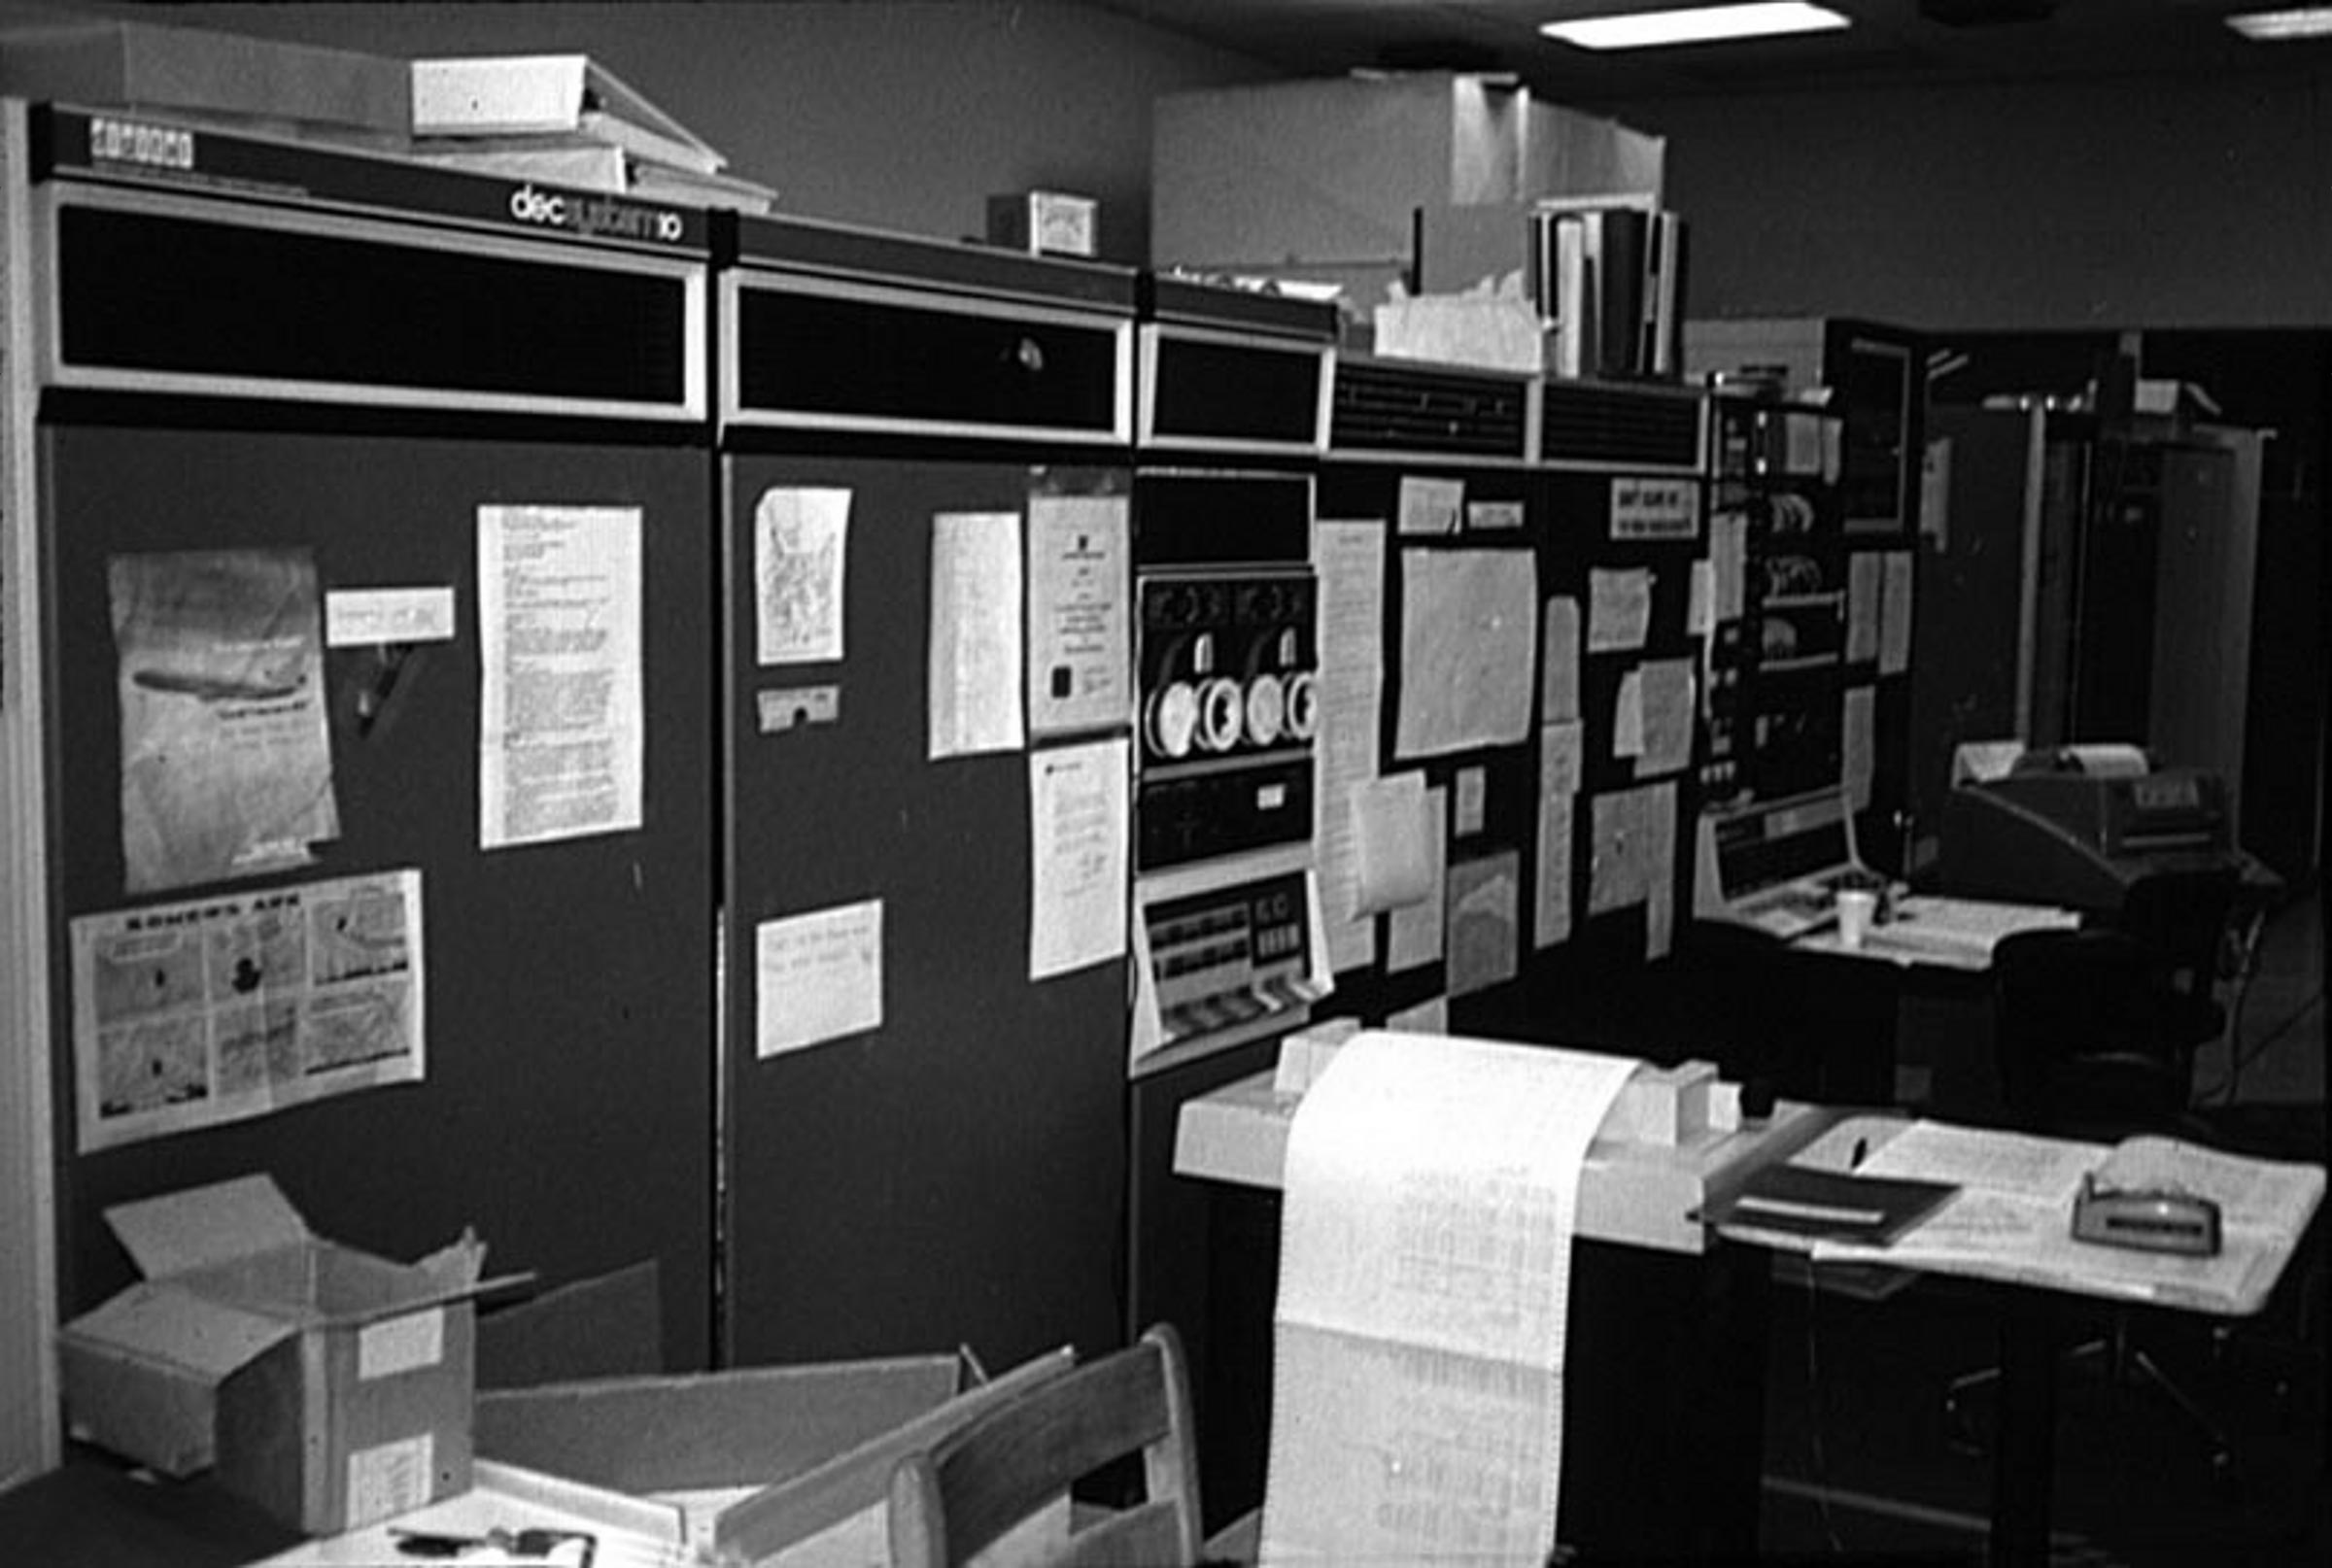
\includegraphics{KL10_1979}
  \caption{PDP-10 processor with KL-10 (a PDP-10 similar to that of the AI Lab), Stanford Artificial Intelligence Laboratory, 1979.}
\end{figure}
\fi

\ifdefined\chs
\begin{figure}[ht] \centering
  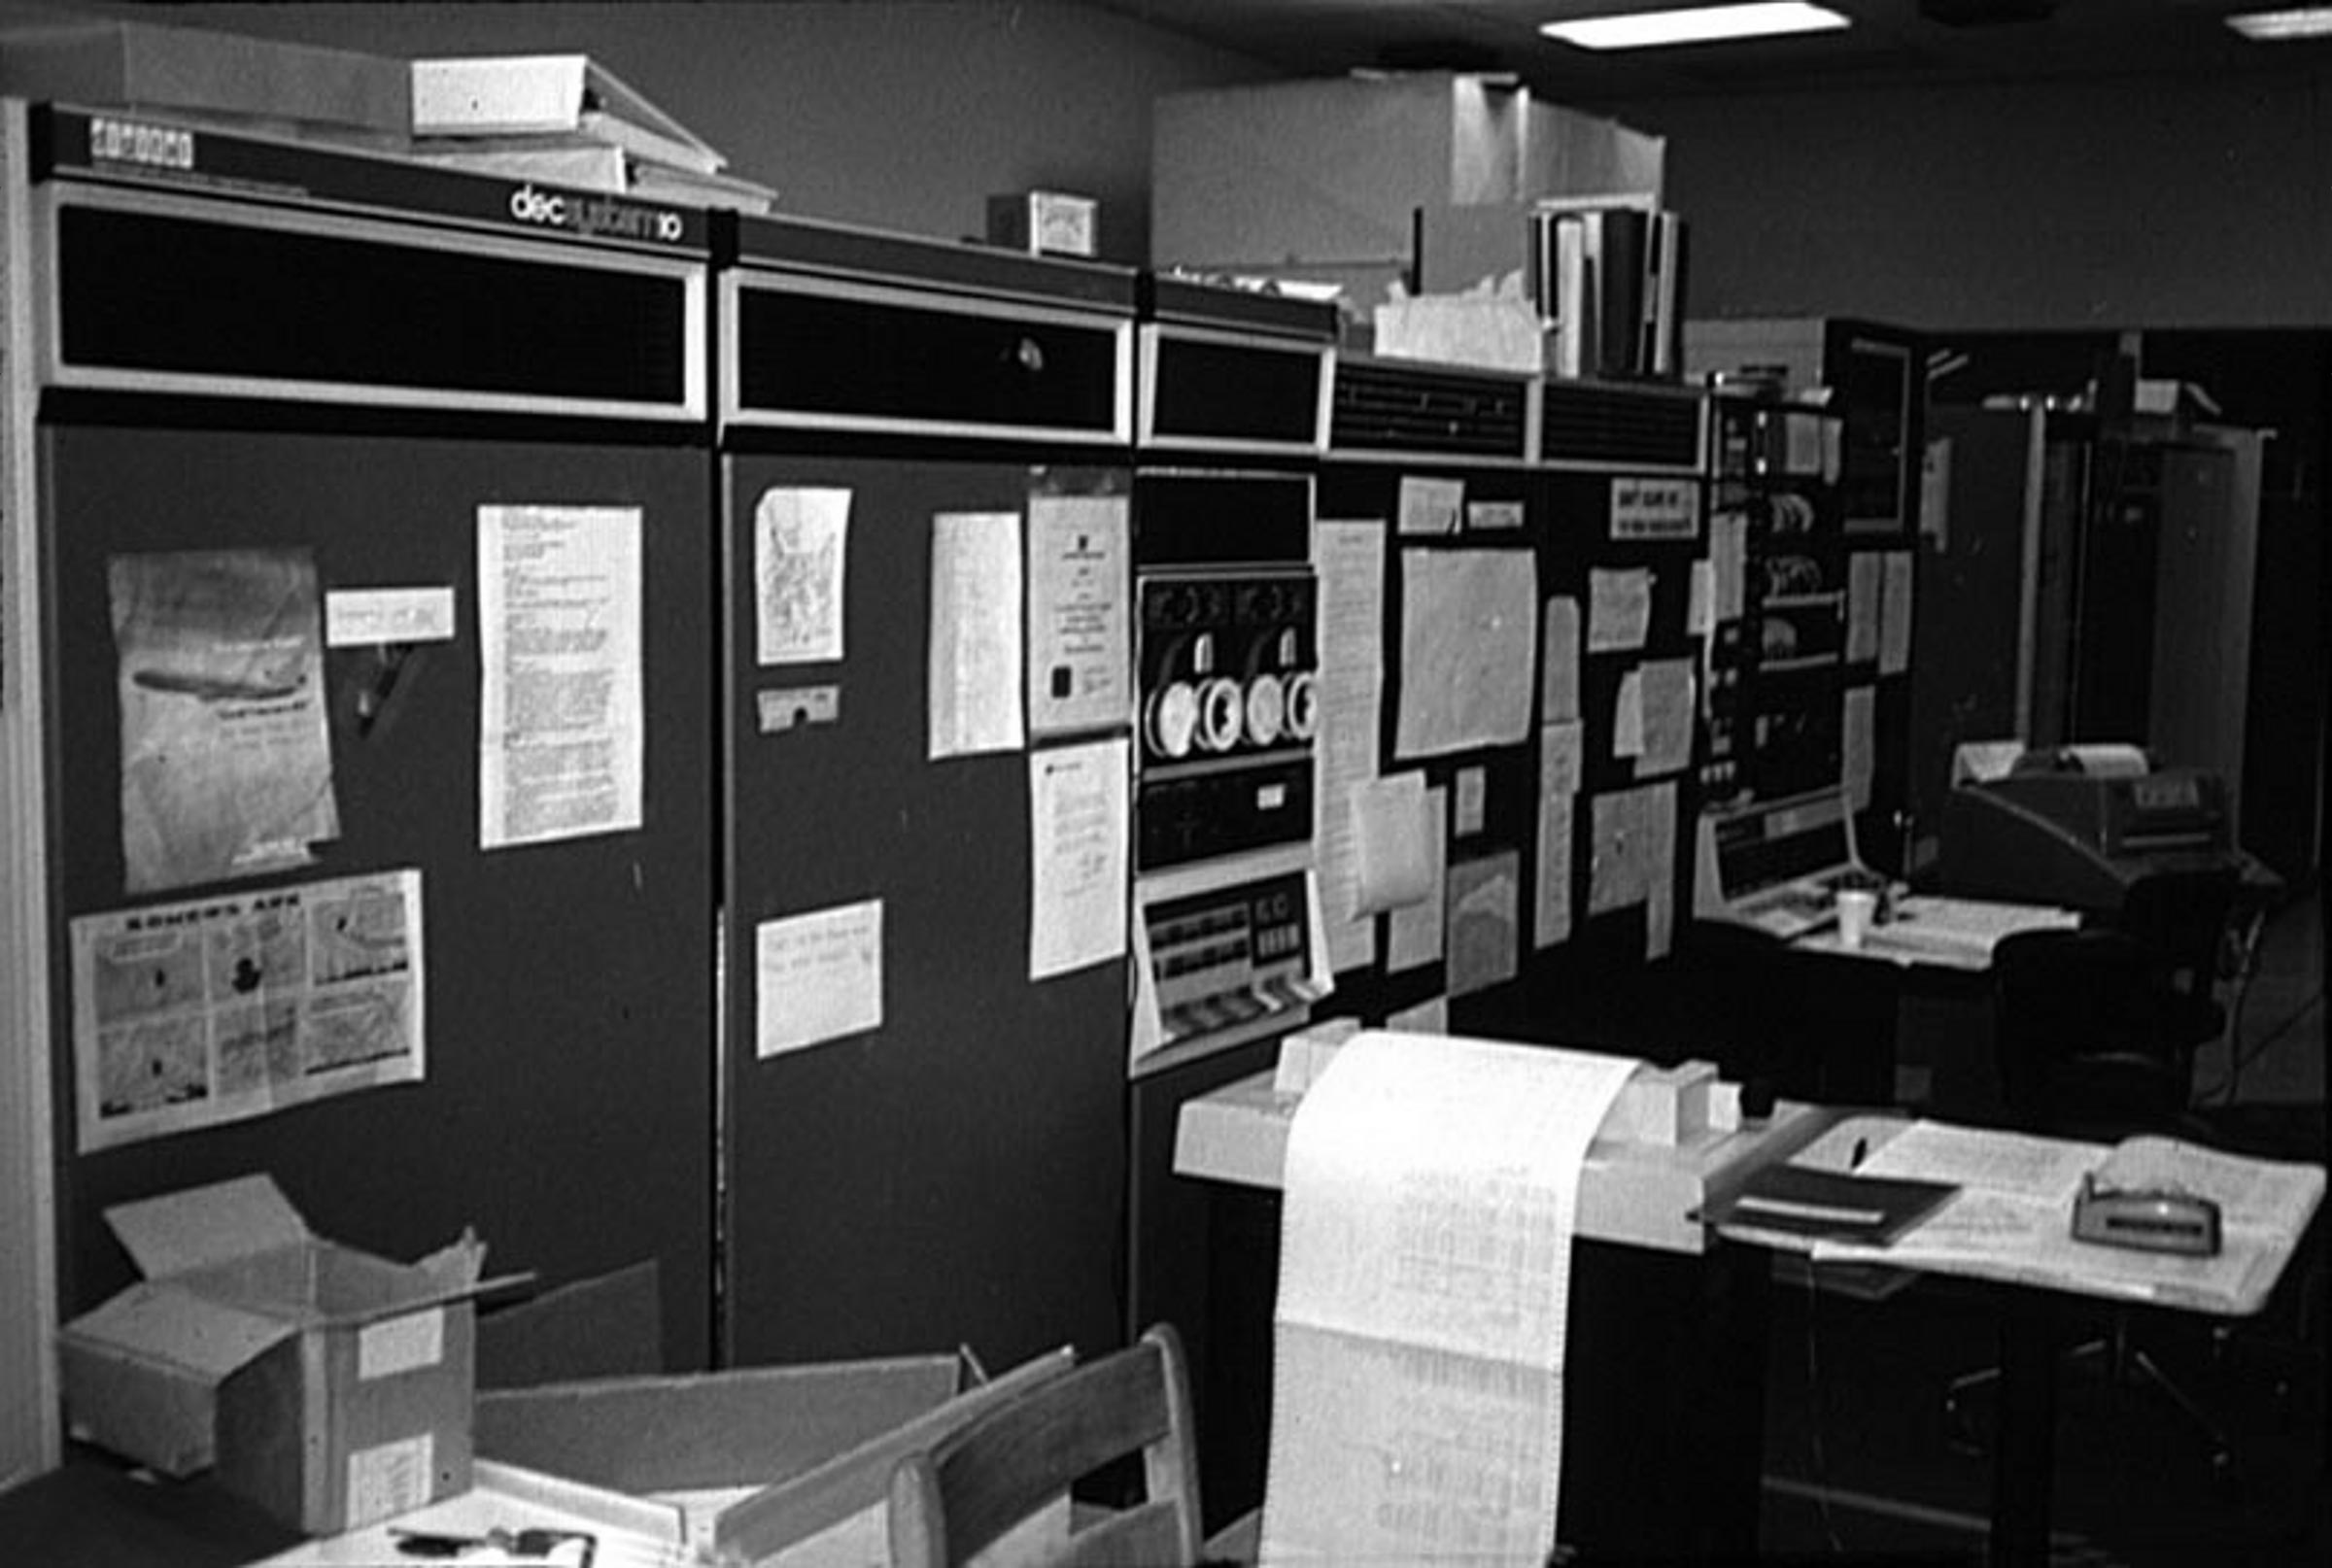
\includegraphics{KL10_1979}
  \caption{PDP-10与KL-10。图片拍摄地点为斯坦福大学人工智能实验室,摄于1979年。}
\end{figure}
\fi
\fi

\ifdefined\eng
``Without hackers to maintain the system, [faculty members] said, `We're going to have a disaster; we must have commercial software,'\hspace{0.01in}'' Stallman would recall a few years later. ``They said, `We can expect the company to maintain it.' It proved that they were utterly wrong, but that's what they did.''\endnote{\textit{Ibid.}}
\fi

\ifdefined\chs
几年之后,斯托曼回忆起那时的情景:``那些教授们说:`没有足够的黑客们来维护ITS系统,我们将会面临各种灾难。要避免这些发生,我们只能投靠商业软件。我们可以让商业公司来提供维护。'后来的事实证明,他们的这番论调大错特错。可当时他们的确这么做了\endnote{\textit{同上。}}。''
\fi

\ifdefined\eng
At first, hackers viewed the Twenex system as yet another authoritarian symbol begging to be subverted. The system's name itself was a protest. Officially dubbed TOPS-20 by DEC, it was \ifdefined\vtwo named\fi as a successor to TOPS-10, a \ifdefined\vone commerical \fi\ifdefined\vtwo proprietary \fi operating system DEC \ifdefined\vone marketed \fi\ifdefined\vtwo distributed \fi for the PDP-10. \ifdefined\vone Bolt Beranek Newman had deveoped an improved version, dubbed Tenex, which TOPS-20 drew upon.\endnote{Multiple sources: see Richard Stallman interview, Gerald Sussman email, and \textit{Jargon File 3.0.0} at \url{http://catb.org/jargon/html/T/TWENEX.html}.} Stallman, \fi\ifdefined\vtwo But TOPS-20 was not based on TOPS-10.  It was derived from the Tenex system which Bolt Beranek Newman had developed for the PDP-10.\endnote{Multiple sources: see Richard Stallman interview, Gerald Sussman email, and \textit{Jargon File 3.0.0} at \url{http://catb.org/jargon/html/T/TWENEX.html}.} Stallman, \fi the hacker who coined the Twenex term, says he came up with the name as a way to avoid using the TOPS-20 name. ``The system was far from tops, so there was no way I was going to call it that,'' Stallman recalls. ``So I decided to insert a `w' in the Tenex name and call it Twenex.''
\fi

\ifdefined\chs
一开始,黑客们觉得Twenex只不过又是一个专制的标志。和之前那些专制标志一样,只要把它推翻,就万事大吉了。这个系统从名字看,就像是对黑客们的挑衅:迪吉多公司对这个系统的官方名字是TOPS-20,意为``顶尖20''。它是TOPS-10的后继产品,而TOPS-10则是迪吉多当年给PDP-10配备的标准系统。不过TOPS-20并非是在TOPS-10基础上做的开发。它的主要代码都继承自BBN公司(Bolt, Beranek and Newman)为PDP-10开发的Tenex系统\endnote{参见《黑话词典3.0.0》 http://catb.org/jargon/html/T/TWENEX.html}。斯托曼则由此把TOPS-20称作Twenex,因为他实在不想用TOPS-20这个名字。他说:``这个系统可根本算不上`顶尖',我说什么也不会这么夸它。所以我在Tenex里添了个字母w,把它叫做Twenex。''
\fi

\ifdefined\eng
The machine that ran the Twenex/TOPS-20 system had its own derisive nickname: Oz. According to one hacker legend, the machine got its nickname because it required a smaller PDP-11 machine to power its terminal. One hacker, upon viewing the KL-10-PDP-11 setup for the first time, likened it to the wizard's bombastic onscreen introduction in the Wizard of Oz. ``I am the great and powerful Oz,'' the hacker intoned. ``Pay no attention to the PDP-11 behind that console.''\endnote{See \url{http://www.as.cmu.edu/~geek/humor/See_Figure_1.txt}.}
\fi

\ifdefined\chs
在黑客界,人们把跑着TOPS系统的Decsystem计算机戏称作Oz,意为``奥兹国''。奥兹国这名字源自《绿野仙踪》这部小说。因为在黑客界,人们都说这样一台计算机需要有个PDP-11作为终端机才能运行。于是,人们看到这台计算机连着PDP-11作为终端,就不禁想到了《绿野仙踪》中那位吹牛皮的奥兹国大法师。黑客们常戏谑道:``我是伟大全能的奥兹国大法师!我可没看到身后那台PDP-11。\endnote{参见\url{http://www.as.cmu.edu/~geek/humor/See_Figure_1.txt}。}''
\fi

\ifdefined\eng
If hackers laughed when they first encountered the KL-10, their laughter quickly died when they encountered Twenex. Not only did Twenex boast built-in security, but the system's software engineers had designed the tools and applications with the security system in mind. What once had been a cat-and-mouse game over passwords in the case of the Laboratory for Computer Science's security system, now became an out-and-out battle over system management. System administrators argued that without security, the Oz system was more prone to accidental crashes. Hackers argued that crashes could be better prevented by overhauling the source code. Unfortunately, the number of hackers with the time and inclination to perform this sort of overhaul had dwindled to the point that the system-administrator argument prevailed.
\fi

\ifdefined\chs
黑客们当年第一次看到Decsystem的时候也许还会借机嘲笑两句,可很快他们就在Twenex面前笑不起来了。Twenex系统增进了系统的安全强度,而且Twenex上的软件也都考虑了各种安全措施。当年,黑客们试图避免设置任何密码和安全设施,那些行为就好像在和管理员玩猫捉老鼠的游戏。而如今,他们面对的,则是一场彻头彻尾的战斗了。系统管理员辩解说,如果没有这些安全设施,Oz系统就随时都会面临崩溃。而黑客们则辩解说,避免崩溃的最好办法,就是公开程序的源代码。遗憾的是,黑客人数上不占优,而且大多数黑客也逐渐失去了当年的那份果断。最终,系统管理员还是胜利了。
\fi

\ifdefined\vtwo
\ifdefined\eng
The initial policy was that any lab member could have the ``wheel privilege'' to bypass security restrictions.  But anyone who had the ``wheel privilege'' could take it away from anyone else, who would then be powerless to restore it.  This state of affairs tempted a small group of hackers to try to seize total control by canceling the ``wheel privilege'' for all but themselves.
\fi

\ifdefined\chs
一开始的政策是,任何一个人工智能实验室的成员,都拥有一个``特权车服务''(wheel privilege),可以用来绕过系统的安全限制。可是,任何有``特权车''的人,都有权吊销别人的``特权车''。这样一来,就促使一小撮黑客总是尝试吊销其他人的特权,借此掌控全局。
\fi
\fi

\ifdefined\eng
\ifdefined\vone
Cadging passwords and deliberately crashing the system in order to glean evidence from the resulting wreckage, Stallman successfully foiled the system administrators' attempt to assert control. After one foiled ``\textit{coup d'etat},'' Stallman issued an alert to the entire AI staff.\endnote{See Richard Stallman (1986).}
\fi
\ifdefined\vtwo
Cadging passwords, and applying the debugger during startup, Stallman successfully foiled these attempts. After the second foiled ``\textit{coup d'état},'' Stallman issued an alert to all the AI Lab personnel.\endnote{See Richard Stallman (1986).}
\fi
\fi

\ifdefined\chs
见得此状,斯托曼破解了密码,利用开机时的调试器,成功破坏了几个这样企图夺权的阴谋。在第二轮``政变''之后,斯托曼向全体人工智能实验室的人发出了警告信\endnote{参见斯托曼在瑞典皇家技术研究所的演讲(1986年10月30日): http://www.gnu.org/philosophy/stallman-kth.html}。
\fi

\ifdefined\eng
``There has been another attempt to seize power,'' Stallman wrote. ``So far, the aristocratic forces have been defeated.'' To protect his identity, Stallman signed the message ``Radio Free OZ.''
\fi

\ifdefined\chs
信中写道:``还有另外一波强大的力量,企图剥夺我们的权利。不过现在,这些官僚们已经暂时被我们打败了。''这是封匿名信,信底的签名是``自由奥兹国电台''。
\fi

\ifdefined\eng
The disguise was a thin one at best. By 1982, Stallman's aversion to passwords and secrecy had become so well known that users outside the AI Laboratory were using his account \ifdefined\vone as a stepping stone to the ARPAnet, the \fi\ifdefined\vtwo\ from around the ARPAnet -- the \fi research-funded computer network that would serve as a foundation for today's Internet. One such ``tourist'' during the early 1980s was Don Hopkins, a California programmer who learned through the hacking grapevine that all an outsider needed to do to gain access to MIT's vaunted ITS system was to log in under the initials RMS and enter the same three-letter monogram when the system requested a password.
\fi

\ifdefined\chs
不过,所谓的匿名信并没把斯托曼挡在幕后。到了1982年,斯托曼关于密码和安全设施的抗议早就内外闻名。以至于有不少人工智能实验室以外的人,通过ARPAnet网络,使用斯托曼的登录帐号,访问人工智能实验室的计算机。他们当初使用的ARPAnet,是如今互联网的雏形。它曾是一个研究项目,旨在构造一个大型计算机网络。这个网络之后不断发展,最终成了今天大家见到的互联网。唐·霍普金斯(Don Hopkins)在八十年代是加利福尼亚州的一名程序员,他当年就曾利用斯托曼的帐号访问人工智能实验室的计算机。他当年从黑客圈的小道消息里听说,想要使用麻省理工学院大名鼎鼎的ITS系统,只需要使用一个简单的用户名和密码登录就可以:用户名,RMS;密码,RMS。
\fi

\ifdefined\eng
``I'm eternally grateful that MIT let me and many other people use their computers for free,'' says Hopkins. ``It meant a lot to many people.''
\fi

\ifdefined\chs
霍普金斯说:``麻省理工学院让我和很多其他的人免费使用他们的计算机,这让我受益终生。这在当时,对大家来说可是份厚礼。``
\fi

\ifdefined\eng
\ifdefined\vone
This so-called ``tourist'' policy, which had been openly tolerated by MIT management during the ITS years,\endnote{See ``MIT AI Lab Tourist Policy.'' \url{http://catalog.com/hopkins/text/tourist-policy.html}} fell by the wayside when Oz became the lab's primary link to the ARPAnet. At first, Stallman continued his policy of repeating his login ID as a password so outside users could follow in his footsteps. Over time, however, the Oz's fragility prompted administrators to bar outsiders who, through sheer accident or malicious intent, might bring down the system. When those same administrators eventually demanded that Stallman stop publishing his password, Stallman, citing personal ethics, refused to do so and ceased using the Oz system altogether.\endnote{See Richard Stallman (1986).}
\fi
\ifdefined\vtwo
This so-called ``tourist'' policy, which had been openly tolerated by MIT management during the ITS years,\endnote{See ``MIT AI Lab Tourist Policy,'' \url{http://www.art.net/~hopkins/Don/text/tourist-policy.html}.} fell by the wayside when Oz became the lab's primary link to the ARPAnet. At first, Stallman continued his policy of repeating his login ID as a password so outside users could have access through his account. Over time, however, Oz's fragility prompted administrators to bar outsiders who, through sheer accident or malicious intent, might bring down the system. When those same administrators eventually demanded that Stallman stop publishing his password, Stallman, citing personal ethics, instead ceased using the Oz system altogether.\endnote{See Richard Stallman (1986).}
\fi
\fi

\ifdefined\chs
这种允许``游客''的政策,在ITS时代还能被麻省理工学院的管理人员容忍\endnote{参见《麻省理工学院人工智能实验室游客守则》 http://www.art.net/~hopkins/Don/text/tourist-policy.html}。可等到Oz成为实验室连接ARPAnet的主节点后,这行为就被逐渐禁止了。一开始,斯托曼依旧使用原来简单的用户名和密码,这样外部人员还是可以访问实验室的计算机。但是脆弱的Oz禁不起这么折腾,很快管理员就禁止了外部人员的访问。因为有些访客会有意无意地把整个系统搞垮。再后来,管理员们严重警告了斯托曼公开用户名和密码的行为。对此,斯托曼并没有放弃使用Oz系统,而是在回应中强调了自己的底线\endnote{参见理查德·斯托曼在瑞典皇家技术研究所的演讲(1986年10月30日): http://www.gnu.org/philosophy/stallman-kth.html}。
\fi

\ifdefined\eng
``[When] passwords first appeared at the MIT AI Lab I [decided] to follow my belief that there should be no passwords,'' Stallman would later say. ``Because I don't believe that it's really desirable to have security on a computer, I shouldn't be willing to help uphold the security regime.''\endnote{\textit{Ibid.}}
\fi

\ifdefined\chs
斯托曼之后说:``当年人工智能实验室第一次要求设置密码,我依旧坚持自己的原则:计算机上不该有密码。我也因此坚决不会帮助他们维护一个充满安全设施的计算机系统。''\endnote{\textit{同上。}}
\fi

\ifdefined\eng
\ifdefined\vone
Stallman's refusal to bow before the great and powerful Oz symbolized the growing tension between hackers and AI Lab management during the early 1980s. This tension paled in comparison to the conflict that raged within the hacker community itself. By the time the KL-10 arrived, the hacker community had already divided into two camps. The first centered around a software company called Symbolics, Inc. The second centered around Symbolics chief rival, Lisp Machines, Inc. (LMI). Both companies were in a race to market the Lisp Machine, a device built to take full advantage of the Lisp programming language.
\fi
\ifdefined\vtwo
Stallman's refusal to bow before the great and powerful Oz symbolized the growing tension between hackers and AI Lab management during the early 1980s. This tension paled in comparison to the conflict that raged within the hacker community itself. By the time the Decsystem 20 arrived, the hacker community was divided into two camps, LMI and Symbolics.
\fi
\fi

\ifdefined\chs
\ifdefined\vone
八十年代早期,斯托曼的这次抗议,标志着黑客和系统管理员之间的矛盾进一步升级。不过随着时间的流逝,这种紧张关系反而被黑客圈子内部的矛盾逐渐取代。在KL-10来到实验室的时候,实验室的黑客圈子已经俨然分成了两派。一派主要围绕一家名为Symbolics的商业软件公司,另一派则围绕Symbolics的对手公司Lisp Machines (LMI)。这两家公司在Lisp机的市场竞争中不分上下,这种Lisp机是以Lisp编程语言为基础构建的。
\fi
\ifdefined\vtwo
八十年代早期,斯托曼的这次抗议,标志着黑客和系统管理员之间的矛盾进一步升级。不过随着时间的流逝,这种紧张关系反而被黑客圈子内部的矛盾逐渐取代。在Decsystem 20来到实验室的时候,实验室的黑客圈子已经俨然分成了两派:LMI派和Symbolics派。
\fi
\fi

\ifdefined\vone
\ifdefined\eng
Created by artificial-intelligence research pioneer John McCarthy, a MIT artificial-intelligence researcher during the late 1950s, Lisp is an elegant language well-suited for programs charged with heavy-duty sorting and processing. The language's name is a shortened version of LISt Processing. Following McCarthy's departure to the Stanford Artificial Intelligence Laboratory, MIT hackers refined the language into a local dialect dubbed MACLISP. The ``MAC'' stood for Project MAC, the DARPA-funded research project that gave birth to the AI Lab and the Laboratory for Computer Science. Led by AI Lab arch-hacker Richard Greenblatt, AI Lab programmers during the 1970s built up an entire Lisp-based operating system, dubbed the Lisp Machine operating system. By 1980, the Lisp Machine project had generated two commercial spin-offs. Symbolics was headed by Russell Noftsker, a former AI Lab administrator, and Lisp Machines, Inc., was headed by Greenblatt.
\fi

\ifdefined\chs
............
\fi

\ifdefined\eng
The Lisp Machine software was hacker-built, meaning it was owned by MIT but available for anyone to copy as per hacker custom. Such a system limited the marketing advantage of any company hoping to license the software from MIT and market it as unique. To secure an advantage, and to bolster the aspects of the operating system that customers might consider attractive, the companies recruited various AI Lab hackers and set them working on various components of the Lisp Machine operating system outside the auspices of the AI Lab.
\fi

\ifdefined\chs
.........
\fi

\ifdefined\eng
The most aggressive in this strategy was Symbolics. By the end of 1980, the company had hired 14 AI Lab staffers as part-time consultants to develop its version of the Lisp Machine. Apart from Stallman, the rest signed on to help LMI.\endnote{}
\fi

\ifdefined\chs
...............
\fi
\fi

\ifdefined\vtwo
\ifdefined\eng
Symbolics, with its outside investment, recruited various AI Lab hackers and set some of them working on improving parts of the Lisp Machine operating system outside the auspices of the AI Lab. By the end of 1980, the company had hired 14 AI Lab staffers as part-time consultants to develop its version of the Lisp Machine. The remaining few, apart from Stallman, worked for LMI.\endnote{See Steve Levy, \textit{Hackers}, page 423.}  Stallman, preferring the unpressured life at the AI Lab and not wishing to take a side, chose to join neither company.
\fi

\ifdefined\chs
LMI和Symbolics分别是两家做Lisp机的计算机公司。Symbolics得到了一些外部的投资,它招募了很多人工智能实验室的黑客,把其中的一部分黑客安排去改进Symbolics的Lisp机的操作系统。八十年代末期,这家公司已经吸纳了人工智能实验室的14位黑客作为兼职顾问,负责开发他们的Lisp机。剩下的黑客们,除了斯托曼以外,则都在LMI公司就职\endnote{参见史蒂芬·李维(Steven Levy),《黑客》(1984年,美国企鹅出版社),第423页。}。斯托曼则更享受人工智能实验室里没有压力的工作环境,更不想把自己划进哪个阵营。所以他哪个公司都没加入。
\fi
\fi

\ifdefined\eng
\ifdefined\vone
At first, Stallman accepted both companies' attempt to commercialize the Lisp machine, even though it meant more work for him. Both licensed the Lisp Machine OS source code from MIT, and it was Stallman's job to update the lab's own Lisp Machine to keep pace with the latest innovations. Although Symbolics' license with MIT gave Stallman the right to review, but not copy, Symbolics' source code, Stallman says a ``gentleman's agreement'' between Symbolics management and the AI Lab made it possible to borrow attractive snippets in traditional hacker fashion.
\fi
\ifdefined\vtwo
At first, the other hackers continued spending some of their time at MIT, and contributed to MIT's Lisp Machine operating system. Both LMI and Symbolics had licensed this code from MIT. The license required them to return their changes to MIT, but did not require them to let MIT redistribute these changes.  However, through 1981 they adhered to a gentleman's agreement to permit that, so all their system improvements were included in the MIT version and thus shared with all Lisp Machine users. This situation allowed those still at MIT to remain neutral.
\fi
\fi

\ifdefined\chs
\ifdefined\vone
.............
\fi
\ifdefined\vtwo
一开始,这些在公司干活的黑客们还会抽出些时间,在麻省理工学院继续做些工作,也会给麻省理工学院的Lisp机的操作系统贡献些代码。LMI和Symbolics的Lisp机操作系统都是从麻省理工学院的Lisp机操作系统上衍生而来。在使用许可证上,麻省理工学院要求两家公司必须允许麻省理工学院使用它们的操作系统。但是,这两家公司可以禁止麻省理工学院再发布他们的产品。不过,1981年间,两家公司之间倒是有个不成文的君子协议,他们都允许麻省理工学院使用并再发布两家公司的代码。这样,麻省理工学院的Lisp机操作系统就包含了来自外部公司的各种改进,而基于许可证,改进后的系统代码又可以继续流入各家公司。这相当于公司之间可以共享代码。如此,那些依旧在麻省理工学院工作的黑客们,就可以继续保持中立。
\fi
\fi

\ifdefined\eng
\ifdefined\vone
On March 16, 1982, a date Stallman remembers well because it was his birthday, Symbolics executives decided to end this gentlemen's agreement. The move was largely strategic. LMI, the primary competition in the Lisp Machine marketplace, was essentially using a copy of the AI Lab Lisp Machine. Rather than subsidize the development of a market rival, Symbolics executives elected to enforce the letter of the license. If the AI Lab wanted its operating system to stay current with the Symbolics operating system, the lab would have to switch over to a Symbolics machine and sever its connection to LMI.
\fi
\ifdefined\vtwo
On March 16, 1982, a date Stallman remembers well because it was his birthday, Symbolics executives ended the gentleman's agreement. The motive was to attack LMI. LMI had fewer hackers, and fewer staff in general, so the Symbolics executives thought that LMI was getting the main benefit of sharing the system improvements.  By ending the sharing of system code, they hoped to wipe out LMI.  So they decided to enforce the letter of the license.  Instead of contributing their improvements to the MIT version of the system, which LMI could use, they provided MIT with a copy of the Symbolics version of the system for users at MIT to run.  Anyone using it would provide the service of testing only to Symbolics, and if he made improvements, most likely they too would only be useful for Symbolics.
\fi
\fi

\ifdefined\chs
\ifdefined\vone
..............
\fi
\ifdefined\vtwo
1982年3月16日,斯托曼清晰地记得这一天,那是他的生日。在这一天,Symbolics的主管们决定不再遵循当初那份君子协议。为了打击LMI,他们禁止麻省理工学院再发布包含Symbolics公司的代码。因为在LMI公司就职的黑客比较少,所以Symbolics的主管们觉得LMI从共享的代码中获益更多。通过切断代码流通的途径,Symbolics企图把LMI赶出市场。为了不让LMI获得自己的代码,他们决定执行许可证上的权利,仅仅允许麻省理工学院的学生运行他们的操作系统。借此,Symbolics可以间接地让学院中的用户为自己做测试。而任何用户提供的代码测试和改进都只能被Symbolics公司所用。
\fi
\fi

\ifdefined\eng
\ifdefined\vone
As the person responsible for keeping up the lab's Lisp Machine, Stallman was incensed. Viewing this announcement as an ``ultimatum,'' he retaliated by disconnecting Symbolics' microwave communications link to the laboratory. He then vowed never to work on a Symbolics machine and pledged his immediate allegiance to LMI. ``The way I saw it, the AI Lab was a neutral country, like Belgium in World War I,'' Stallman says. ``If Germany invades Belgium, Belgium declares war on Germany and sides with Britain and France.''
\fi
\ifdefined\vtwo
As the person responsible (with help from Greenblatt for the first couple of months) for keeping up the lab's Lisp Machine system, Stallman was incensed. The Symbolics hackers had left the system code with hundreds of half-made changes that caused errors. Viewing this announcement as an ``ultimatum,'' he retaliated by disconnecting Symbolics' microwave communications link to the laboratory. He then vowed never to work on a Symbolics machine, and pledged to continue the development of MIT's system so as to defend LMI from Symbolics. ``The way I saw it, the AI Lab was a neutral country, like Belgium in World War II,'' Stallman says. ``If Germany invades Belgium, Belgium declares war on Germany and sides with Britain and France.''
\fi
\fi

\ifdefined\chs
\ifdefined\vone
..............
\fi
\ifdefined\vtwo
斯托曼在那时候负责维护实验室中的Lisp机,最开始的几个月还多亏了LMI公司的创始人,格林布拉特(Greenblatt)的指点帮助。当下,Symbolics的做法可是惹恼了斯托曼。那些在Symbolics公司工作的黑客们都曾给实验室的Lisp机系统贡献过代码,如今,还有很多错误和bug遗留在这些代码中,甚至有些特性还都是半成品。如今,Symbolics高层的做法无疑相当于下了``最后通牒'',令身在Symbolics的黑客们无法改进麻省理工学院的Lisp机系统。斯托曼也发起了反攻,他切断了连接实验室和Symbolics公司的微波通信信道,发誓再也不会在Symbolics生产的机器上工作。并且决心要继续完善麻省理工学院的Lisp机系统上,以此帮助LMI,打击Symbolics。斯托曼回忆说:``当初我觉得,人工智能实验室是个中立国,就好像二战时的比利时一样。如果德国入侵比利时,比利时就要对德宣战,就得和英法一个阵营。''
\fi
\fi

\ifdefined\vone
\ifdefined\eng
The circumstances of the so-called ``Symbolics War'' of 1982-1983 depend heavily on the source doing the telling. When Symbolics executives noticed that their latest features were still appearing in the AI Lab Lisp Machine and, by extension, the LMI Lisp machine, they installed a ``spy'' program on Stallman's computer terminal. Stallman says he was rewriting the features from scratch, taking advantage of the license's review clause but also taking pains to make the source code as different as possible. Symbolics executives argued otherwise and took their case to MIT administration. According to 1994 book, The Brain Makers: Genius, Ego, and Greed, and the Quest for Machines That Think, written by Harvey Newquist, the administration responded with a warning to Stallman to ``stay away'' from the Lisp Machine project.8 According to Stallman, MIT administrators backed Stallman up. ``I was never threatened,'' he says. ``I did make changes in my practices, though. Just to be ultra safe, I no longer read their source code. I used only the documentation and wrote the code from that.''
\fi

\ifdefined\chs
.............
\fi

\ifdefined\eng
Whatever the outcome, the bickering solidified Stallman's resolve. With no source code to review, Stallman filled in the software gaps according to his own tastes and enlisted members of the AI Lab to provide a continuous stream of bug reports. He also made sure LMI programmers had direct access to the changes. ``I was going to punish Symbolics if it was the last thing I did,'' Stallman says.
\fi

\ifdefined\chs
...........
\fi

\ifdefined\eng
Such statements are revealing. Not only do they shed light on Stallman's nonpacifist nature, they also reflect the intense level of emotion triggered by the conflict. According to another Newquist-related story, Stallman became so irate at one point that he issued an email threatening to ``wrap myself in dynamite and walk into Symbolics' offices.''9 Although Stallman would deny any memory of the email and still describes its existence as a ``vicious rumor,'' he acknowledges that such thoughts did enter his head. ``I definitely did have fantasies of killing myself and destroying their building in the process,'' Stallman says. ``I thought my life was over.''\endnote{}
\fi

\ifdefined\chs
............
\fi
\fi

\ifdefined\vtwo
\ifdefined\eng
When Symbolics executives noticed that their latest features were still appearing in the MIT Lisp Machine system and, by extension, the LMI Lisp machine, they were not pleased. Stallman knew what copyright law required, and was rewriting the features from scratch.  He took advantage of the opportunity to read the source code Symbolics supplied to MIT, so as to understand the problems and fixes, and then made sure to write his changes in a totally different way.  But the Symbolics executives didn't believe this.  They installed a ``spy'' program on Stallman's computer terminal looking for evidence against him.  However, when they took their case to MIT administration, around the start of 1983, they had little evidence to present: a dozen places in the sources where both versions had been changed and appeared similar.
\fi

\ifdefined\chs
Symbolics公司的主管们逐渐意识到,自己公司操作系统的最新特性,总会依旧出现在麻省理工学院的Lisp机系统上,甚至是LMI的Lisp机系统中。这让他们甚为不满。斯托曼知道版权法这么个东西,所以他为学院的系统添加的特性,都是自己从头开始写的。他身在人工智能实验室,可以读到Symbolics操作系统提供给实验室的源代码。他会先读读Symbolics的代码,理解要解决的问题和解决方案,最后再自己重新写一遍,确保和Symbolics的实现完全不同。可Symbolics公司的主管们却不管这个。他们在斯托曼使用的计算机终端上安装了间谍软件,企图抓住斯托曼剽窃的证据。到了1983年年初,他们把这件事情告到麻省理工学院的管理层。可依旧拿不出多少像样的证据,只有一些看似类似的代码片段。
\fi

\ifdefined\eng
When the AI Lab administrators showed Stallman Symbolics' supposed evidence, he refuted it, showing that the similarities were actually held over from before the fork.  Then he turned the logic around: if, after the thousands of lines he had written, Symbolics could produce no better evidence than this, it demonstrated that Stallman's diligent efforts to avoid copying were effective.  The AI Lab approved Stallman's work, which he continued till the end of 1983.\endnote{\textit{The Brain Makers} by H. P. Newquist says inaccurately that the AI Lab told Stallman to stay away from the Lisp Machine project.}
\fi

\ifdefined\chs
人工智能实验室的主管找来斯托曼,给他看了Symbolics公司指责他的证据。斯托曼一一否认,他说这些相似的代码都是Symbolics诞生之前,在学院Lisp系统里就有的。之后,斯托曼话锋一转:他自己已经克隆了Symbolics公司的众多特性,在那几千行的代码中,如今Symbolics公司却只能提供这么点证据来证明斯托曼剽窃,这恰恰说明斯托曼的确没有抄袭Symbolics的代码。人工智能实验室最终承认了斯托曼并没有剽窃,他也就继续开发到1983年\endnote{N. P. 纽奎斯特所 (N. P. Newquist)所著的《大脑创作家》(The Brain Maker)一书中说,人工智能实验室实验室警告斯托曼,让他从此远离Lisp机项目。此说法后被证伪。}。
\fi

\ifdefined\eng
Stallman did make a change in his practices, though.  ``Just to be ultra safe, I no longer read their source code [for new features and major changes]. I used only the documentation and wrote the code from that.''  For the biggest new features, rather than wait for Symbolics to release documentation, he designed them on his own; later, when the Symbolics documentation appeared, he added compatibility with Symbolics' interface for the feature.  Then he read Symbolics' source code changes to find minor bugs they had fixed, and fixed each of them differently.
\fi

\ifdefined\chs
不过这件事倒是确实给斯托曼提了醒。``以防万一,对于新的特性和重大改变,我不再参考Symbolics的代码,而只是参考他们提供的用户文档来做开发。''对于一些重大的新特性,斯托曼则往往在文档发布之前就着手设计开发。等到Symbolics公司发布文档,他再对代码修改,以便兼容Symbolics的接口。之后,如果Symbolics提供了补丁,他再阅读补丁的代码,以便确认自己的实现中是否存在类似bug。如果存在,则尝试用不同的实现来解决。
\fi

\ifdefined\eng
The experience solidified Stallman's resolve. As Stallman designed replacements for Symbolics' new features, he also enlisted members of the AI Lab to keep using the MIT system, so as to provide a continuous stream of bug reports. MIT continued giving LMI direct access to the changes. ``I was going to punish Symbolics if it was the last thing I did,'' Stallman says.  Such statements are revealing. Not only do they shed light on Stallman's nonpacifist nature, they also reflect the intense level of emotion triggered by the conflict.
\fi

\ifdefined\chs
整个过程也坚定了斯托曼的决心。斯托曼的开发,逐渐把人工智能实验室中的成员拉回到麻省理工学院的Lisp机系统上。这些用户也为斯托曼持续地提供错误报告。麻省理工学院继续允许LMI直接访问学院Lisp机系统的代码。斯托曼说:``我当初就觉得,我要是这辈子只能再做一件事,那就是要惩罚Symbolics。''这话说得甚是坦白。显然,斯托曼不是个和平主义者。随着矛盾的升级,给双方带来的情感变化也逐渐加大。
\fi
\fi

\ifdefined\eng
\ifdefined\vone
The level of despair owed much to what Stallman viewed as the ``destruction'' of his ``home''-i.e., the demise of the AI Lab's close-knit hacker subculture. In a later email interview with Levy, Stallman would liken himself to the historical figure Ishi, the last surviving member of the Yahi, a Pacific Northwest tribe wiped out during the Indian wars of the 1860s and 1870s. The analogy casts Stallman's survival in epic, almost mythical, terms. In reality, however, it glosses over the tension between Stallman and his fellow AI Lab hackers prior to the Symbolics-LMI schism. Instead of seeing Symbolics as an exterminating force, many of Stallman's colleagues saw it as a belated bid for relevance. In commercializing the Lisp Machine, the company pushed hacker principles of engineer-driven software design out of the ivory-tower confines of the AI Lab and into the corporate marketplace where manager-driven design principles held sway. Rather than viewing Stallman as a holdout, many hackers saw him as a troubling anachronism.
\fi
\ifdefined\vtwo
The level of despair owed much to what Stallman viewed as the ``destruction'' of his ``home'' -- i.e., the demise of the AI Lab's close-knit hacker subculture. In a later email interview with Levy, Stallman would liken himself to the historical figure Ishi, the last surviving member of the Yahi, a Pacific Northwest tribe wiped out during the Indian wars of the 1860s and 1870s. The analogy casts Stallman's survival in epic, almost mythical, terms.\endnote{Steven Levy in \textit{Hackers} had this period in mind when he described Stallman as the ``last of the true hackers,'' but his intended meaning was not what you might think.  Levy used the term ``true hackers'' to distinguish the MIT hacker community from two other hacker communities described later in the book, to which he gave other names. When this community had dissolved, leaving only Stallman, he therefore became the last of the ``true hackers.''   Levy did not mean that nobody else was truly a hacker, but people tend to interpret his words that way, especially those who see them without reading the explanations in Levy's book.  Stallman has never described himself using those words of Levy's.} The hackers who worked for Symbolics saw it differently. Instead of seeing Symbolics as an exterminating force, many of Stallman's colleagues saw it as a belated bid for relevance. In commercializing the Lisp Machine, the company pushed hacker principles of engineer-driven software design out of the ivory-tower confines of the AI Lab and into the corporate marketplace where manager-driven design principles held sway. Rather than viewing Stallman as a holdout, many hackers saw him as the representative of an obsolete practice.
\fi
\fi

\ifdefined\chs
\ifdefined\vone
.............
\fi
\ifdefined\vtwo
由此带来的绝望感,让斯托曼又有了家园被毁的感受。人心散了,人工智能实验室的黑客文化也逐渐褪去。之后在与史蒂芬·李维的采访邮件中,斯托曼把自己形容为Ishi——加利福尼亚州最后一位Yahi族印第安人。这样的说法倒是为斯托曼的经历凭添了几分史诗色彩\endnote{史蒂芬·李维(Steven Levy)在《黑客》一书中,称斯托曼为``最后一位真正黑客''。不过李维的这个称呼经常被人误解。李维在书中使用``真正黑客''一词来专指麻省理工学院的黑客们。以此来和其他黑客社区区分。当麻省理工学院的黑客文化逐渐消退,只剩下斯托曼一个人的时候,他显然就被称为``最后一位真正黑客''了。李维并非想说,除了斯托曼以外,别人都算不上黑客。但是后人常常以此解读,特别人那些没有读过《黑客》一书的人。斯托曼自己也从不用这一称呼来形容自己。}。不过在Symbolics工作的各位黑客们则另有看法。他们并非觉得Symbolics好像要上灭下绝。很多斯托曼当年的同事,都觉得Symbolics倒是迟到的正义。在把Lisp机商业化的过程中,Symbolics把黑客文化中的``工程师做主''的原则从象牙塔中带入了商业公司里,让公司里不再有``外行领导内行``的现象。其他黑客们也没觉得斯托曼是在捍卫什么,而是觉得他只是代表着一种过时的想法而已。
\fi
\fi




\ifdefined\eng
\ifdefined\vone
Stallman does not dispute this alternate view of historical events. In fact, he says it was yet another reason for the hostility triggered by the Symbolics ``ultimatum.'' Even before Symbolics hired away most of the AI Lab's hacker staff, Stallman says many of the hackers who later joined Symbolics were shunning him. ``I was no longer getting invited to go to Chinatown,'' Stallman recalls. ``The custom started by Greenblatt was that if you went out to dinner, you went around or sent a message asking anybody at the lab if they also wanted to go. Sometime around 1980-1981, I stopped getting asked. They were not only not inviting me, but one person later confessed that he had been pressured to lie to me to keep their going away to dinner without me a secret.''
\fi
\ifdefined\vtwo
Personal hostilities also affected the situation.   Even before Symbolics hired away most of the AI Lab's hacker staff, Stallman says many of the hackers who later joined Symbolics were shunning him. ``I was no longer getting invited to go to Chinatown,'' Stallman recalls. ``The custom started by Greenblatt was that if you went out to dinner, you went around or sent a message asking anybody at the lab if they also wanted to go. Sometime around 1980-1981, I stopped getting asked. They were not only not inviting me, but one person later confessed that he had been pressured to lie to me to keep their going away to dinner without me a secret.''
\fi
\fi

\ifdefined\chs
\ifdefined\vone
............
\fi
\ifdefined\vtwo
私下的过结也让事态趋于严重。斯托曼说,Symbolics公司雇走大量黑客之前,斯托曼就觉得很多黑客都在有意躲避自己。这些黑客之后大部分都加入了Symbolics公司。斯托曼回忆:``他们很少问我去不去唐人街吃饭了。当年从格林布拉特(Greenblatt)开始,实验室就有个传统:谁要是去吃饭,谁就发个消息或者亲自走一圈,问问实验室里还有谁想一起去。可大概在1980年到1981年间,逐渐就没什么人问我了。他们不邀请我倒也罢了。之后,他们之中有人才告诉我,当年他被人告之,不许他跟我说大家一起出去吃饭故意不带我这个事。''
\fi
\fi

\ifdefined\eng
\ifdefined\vone
Although Stallman felt anger toward the hackers who orchestrated this petty form of ostracism, the Symbolics controversy dredged up a new kind of anger, the anger of a person about to lose his home. When Symbolics stopped sending over its source-code changes, Stallman responded by holing up in his MIT offices and rewriting each new software feature and tool from scratch. Frustrating as it may have been, it guaranteed that future Lisp Machine users had unfettered access to the same features as Symbolics users.
\fi
\ifdefined\vtwo
Although Stallman felt hurt by this petty form of ostracism, there was nothing to be done about it.  The Symbolics ultimatum changed the matter from a personal rejection to a broader injustice. When Symbolics excluded its source changes from redistribution, as a means to defeat its rival, Stallman determined to thwart Symbolics' goal. By holing up in his MIT offices and writing equivalents for each new software feature and fix, he gave users of the MIT system, including LMI customers, access to the same features as Symbolics users.
\fi
\fi

\ifdefined\chs
\ifdefined\vone
.............
\fi
\ifdefined\vtwo
虽然斯托曼对这种排斥行为非常反感,但并没对此有什么行动。可Symbolics的最后通牒则改变了一切,这事从此也不再是私人恩怨了。当Symbolics公司不再给用户提供源代码的时候,斯托曼决心要对此进行反击。他日夜坐在他的办公室里,在麻省理工学院的Lisp机系统上,实现了Symbolics提供的各种新功能和bug修正。他把修改后的版本代码分发给各个用户,包括LMI公司的客户。这样,LMI公司的客户也可以拥有Symbolics系统类似的功能。
\fi
\fi

\ifdefined\eng
It also guaranteed Stallman's legendary status within the hacker community. Already renowned for his work with Emacs, Stallman's ability to match the output of an entire team of Symbolics programmers -- a team that included more than a few legendary hackers itself -- still stands as one of the major human accomplishments of the Information Age, or of any age for that matter. Dubbing it a ``master hack'' and Stallman himself a ``virtual John Henry of computer code,'' author Steven Levy notes that many of his Symbolics-employed rivals had no choice but to pay their idealistic former comrade grudging respect. Levy quotes Bill Gosper, a hacker who eventually went to work for Symbolics in the company's Palo Alto office, expressing amazement over Stallman's output during this period:
\fi

\ifdefined\chs
这也为斯托曼在黑客圈子里凭添了几分名气。斯托曼早就因为Emacs而名声大噪。如今,他一个人单枪匹马,对抗整个Symbolics公司的开发团队,而且这团队之中还尽是各色传奇黑客。斯托曼的这一行为本身,就足以成为信息时代的一段传奇。史蒂芬·李维在《黑客》一书中称这一行为是``黑客杰作'';并把斯托曼比作现代的约翰·亨利(John Henry)\endnote{译注:约翰·亨利(John Henry),非裔美国人,钢钻工人。传说中他身高力大,曾在19世纪末期参与修筑贯穿美国东西海岸的铁路。期间为保住自己和工友的工作职位,一人单挑一台蒸汽机钻。最终获胜,但因体力透支而离世。约翰·亨利从此成为美国工人勤奋,坚毅的象征。他的画像甚至还出现在二战期间,美国的宣传画册上。}。史蒂芬·李维在书中说,很多Symbolics公司工作的黑客们都钦佩斯托曼的能力。他引述了比尔·高斯伯(Bill Gosper),他曾在Symbolics的帕罗奥多(Palo Alto)分部工作,对于斯托曼那段时期的产出,比尔·高斯伯甚是惊奇:
\fi

\ifdefined\eng
\begin{quote}
I can see something Stallman wrote, and I might decide it was bad (probably not, but somebody could convince me it was bad), and I would still say, ``But wait a minute -- Stallman doesn't have anybody to argue with all night over there. He's working alone! It's incredible anyone could do this alone!''\endnote{See Steven Levy, \textit{Hackers} (Penguin USA [paperback], 1984): 426}
\end{quote}
\fi

\ifdefined\chs
\begin{quote}
我读过斯托曼那段时期的一些代码,有些代码写的并不怎么出色(至少在我看来),但我还是要说:``且慢,他就只有一个人,他没法和别人整晚探讨,他是单枪匹马啊!一个人能完成如此大量的工作,简直是逆天了\endnote{参见史蒂芬·李维(Steven Levy),《黑客》(1984年,美国企鹅出版社),第426页。}!''
\end{quote}
\fi

\ifdefined\eng
For Stallman, the months spent playing catch up with Symbolics evoke a mixture of pride and profound sadness. As a dyed-in-the-wool liberal whose father had served in World War II, Stallman is no pacifist. In many ways, the Symbolics war offered the rite of passage toward which Stallman had been careening ever since joining the AI Lab staff a decade before. At the same time, however, it coincided with the traumatic destruction of the AI Lab hacker culture that had nurtured Stallman since his teenage years. One day, while taking a break from writing code, Stallman experienced a traumatic moment passing through the lab's equipment room. There, Stallman encountered the hulking, unused frame of the PDP-10 machine. Startled by the dormant lights, lights that once actively blinked out a silent code indicating the status of the internal program, Stallman says the emotional impact was not unlike coming across a beloved family member's well-preserved corpse.
\fi

\ifdefined\chs
对于斯托曼来说,这段时期和Symbolics的竞争,既让他感到骄傲,又让他感到了深深的难过。斯托曼是个彻头彻尾的自由主义者,自己的父亲也曾在二战期间为自由而战。他不会期盼勉强得来的和平。在加入人工智能实验室之前,他本就心向自由。如今与Symbolics之间燃起的硝烟,则又把他推向了一个极端。无巧不成书,这次的矛盾,恰恰发生在人工智能实验室黑客文化消退的时候。斯托曼曾被这文化滋润,如今眼见它消失殆尽,其中心酸,难以言表。曾有一日,在他编程的间歇,偶尔路过实验室的设备间。眼见那台曾在实验室服役的PDP-10摆放在房间之中,无人问津。当年那几个忙碌闪烁的状态灯,如今也黯淡无光。往事片段,涌上心头。眼看着这台几十年前的计算机,仿佛看着家中亲人,静静地躺放在那里,魂归西天。
\fi

\ifdefined\eng
``I started crying right there in the \ifdefined\vone equipment \fi\ifdefined\vtwo machine \fi room,'' he says. ``Seeing the machine there, dead, with nobody left to fix it, it all drove home how completely my community had been destroyed.''
\fi

\ifdefined\chs
``我当时泪如泉涌。''斯托曼说,``它就在那儿,可却没人关心,无人维护。眼前的一切在告诉我,我们当年的那个黑客大家庭,早就不复存在了。''
\fi

\ifdefined\eng
Stallman would have little opportunity to mourn. The Lisp Machine, despite all the furor it invoked and all the labor that had gone into making it, was merely a sideshow to the large battles in the technology marketplace. The relentless pace of computer miniaturization was bringing in newer, more powerful microprocessors that would soon incorporate the machine's hardware and software capabilities like a modern metropolis swallowing up an ancient desert village.
\fi

\ifdefined\chs
然而,留给斯托曼感伤怀古的时间却并不多了。无论曾投入过多少人力物力,整个Lisp机产业却仅仅是昙花一现。计算机小型化的脚步一步不停。带来了更新,更强大的微处理器。这一波趋势,如同风卷残云般,将其他竞争者一举赶出主流市场。
\fi

\ifdefined\eng
Riding atop this microprocessor wave were hundreds -- thousands -- of \ifdefined\vone commercial \fi\ifdefined\vtwo proprietary \fi software programs, each protected by a patchwork of user licenses and nondisclosure agreements that made it impossible for hackers to review or share source code. The licenses were crude and ill-fitting, but by 1983 they had become strong enough to satisfy the courts and scare away would-be interlopers. Software, once a form of garnish most hardware companies gave away to make their expensive computer systems more flavorful, was quickly becoming the main dish. In their increasing hunger for new games and features, users were putting aside the traditional demand to review the recipe after every meal.
\fi

\ifdefined\chs
伴随这波风潮而来的,是成千上万的专有软件。每个专有软件,都带着自己的使用许可证和保密协议扑向用户。令其他黑客无法触碰其中的代码。很多软件使用许可证对用户粗暴无礼。但是在1983年,这些专有软件依旧成了主流,填补了市场。也让潜在的竞争对手望而却步。软件,曾经一度只是各个硬件厂商的随机赠品,如今却成了业界新宠。当下,用户们开始极度索要新软件,新功能;而至于是否可以知道软件内部究竟做了什么,则甚少提及。
\fi

\ifdefined\eng
Nowhere was this state of affairs more evident than in the realm of personal computer systems. Companies such as Apple Computer and Commodore were minting fresh millionaires selling machines with built-in operating systems. Unaware of the hacker culture and its distaste for binary-only software, many of these users saw little need to protest when these companies failed to attach the accompanying source-code files. A few anarchic adherents of the hacker ethic helped propel that ethic into this new marketplace, but for the most part, the marketplace rewarded the programmers speedy enough to write new programs and savvy enough to \ifdefined\vone copyright them as legally protected works.\fi\ifdefined\vtwo write End User License Agreements to lock them up tight.\fi
\fi

\ifdefined\chs
个人计算机的到来把这股潮流推向了巅峰。苹果,Commodore等公司跨入了百万富翁的行列。它们出售个人计算机,并在上面安装了自己公司的操作系统。这些计算机的用户们可不再像当年的黑客,他们并不关心软件的源代码,要是买来的软件不附带源代码,他们也不会大呼小叫。一些还恪守当年黑客信条的人,曾试图把黑客的这种传统带入个人计算机这个新兴市场。但无论如何,这个唯利是图的新兴市场推动着程序员写出更多的软件,也同时带来了更多的使用许可证。
\fi

\ifdefined\eng
One of the most notorious of these programmers was Bill Gates, a Harvard dropout two years Stallman's junior. Although Stallman didn't know it at the time, seven years before sending out his message to thenet.unix-wizards newsgroup, Gates, a budding entrepreneur and general partner with the Albuquerque-based software firm Micro-Soft, later spelled as Microsoft, had sent out his own open letter to the software-developer community. Written in response to the PC users copying Micro-Soft's software programs, Gates' ``Open Letter to Hobbyists'' had excoriated the notion of communal software development.
\fi

\ifdefined\chs
这其中,最为著名的程序员恐怕要算比尔·盖茨了。这位哈佛的辍学生比斯托曼小两年入学哈佛,算是斯托曼的学弟。不过斯托曼当年并不认识他。1983年9月27日,斯托曼在thenet.unix-wizards新闻组上发布了GNU工程计划。而七年之前,比尔·盖茨在软件开发者的社区中发表了那封著名的公开信。当年,微软还是坐落在新墨西哥州,阿尔伯克基市的一家小公司。那时,曾有很多PC用户私下拷贝微软的软件。由此,才让比尔·盖茨发表了那封《致爱好者的公开信》。
\fi

\ifdefined\eng
``Who can afford to do professional work for nothing?'' asked Gates. ``What hobbyist can put three man-years into programming, finding all bugs, documenting his product, and distributing it for free?''\endnote{See Bill Gates, ``An Open Letter to Hobbyists'' (February 3, 1976). To view an online copy of this letter, go to \url{http://en.wikipedia.org/wiki/Open_Letter_to_Hobbyists}.}
\fi

\ifdefined\chs
``有谁会在没有任何报酬的情况下来做这些专业工作?''比尔·盖茨在信中发问:``什么样的爱好者可以为他的产品投入三人年\endnote{译注:人年(man-year)软件开发用的单位,用户衡量软件开发的投入精力。假定每个开发人员的能力相同,那么3人年就指三人一年,或一人三年的工作成果。}的精力,开发完软件还得去发现错误,编写文档,最后还要免费发布他的产品\endnote{参见比尔·盖茨1976年2月3日发表的《致爱好者的公开信》。 \url{http://en.wikipedia.org/wiki/Open_Letter_to_Hobbyists}}?''
\fi

\ifdefined\eng
Although few hackers at the AI Lab saw the missive, Gates' 1976 letter nevertheless represented the changing attitude toward software both among commercial software companies and commercial software developers. Why treat software as a zero-cost commodity when the market said otherwise? As the 1970s gave way to the 1980s, selling software became more than a way to recoup costs; it became a political statement. At a time when the Reagan Administration was rushing to dismantle many of the federal regulations and spending programs that had been built up during the half century following the Great Depression, more than a few software programmers saw the hacker ethic as anticompetitive and, by extension, un-American. At best, it was a throwback to the anticorporate attitudes of the late 1960s and early 1970s. Like a Wall Street banker discovering an old tie-dyed shirt hiding between French-cuffed shirts and double-breasted suits, many computer programmers treated the hacker ethic as an embarrassing reminder of an idealistic age.
\fi

\ifdefined\chs
比尔·盖茨1976年2月发表了这封公开信,那会还没有几个人工智能实验室的黑客读过这信。可显然,这封信代表了商业软件公司和软件开发者对于软件态度的转变。既然市场都这么说了,那还为什么把软件当作免费赠品呢?从七十年代走到八十年代,出售软件已经不再仅仅为了弥补开发的成本,它变成了一种政治宣言。当年,里根政府正在极力清除大萧条时期政府制定的各种避免竞争的限制,越来越多的程序员也把黑客文化视为一种反对竞争,乃至违背美国精神的东西。最起码,他们觉得所谓黑客精神,最多是股复古风,不过是六七十年代反对大型企业态度的延续,一种企盼回到理想年代的情结。
\fi

\ifdefined\eng
\ifdefined\vone
For a man who had spent the entire 1960s as an embarrassing throwback to the 1950s, Stallman didn't mind living out of step with his peers. As a programmer used to working with the best machines and the best software, however, Stallman faced what he could only describe as a ``stark moral choice'': either get over his ethical objection for `` proprietary'' software-the term Stallman and his fellow hackers used to describe any program that carried private copyright or end-user license that restricted copying and modification-or dedicate his life to building an alternate, nonproprietary system of software programs. Given his recent months-long ordeal with Symbolics, Stallman felt more comfortable with the latter option. ``I suppose I could have stopped working on computers altogether,'' Stallman says. ``I had no special skills, but I'm sure I could have become a waiter. Not at a fancy restaurant, probably, but I could've been a waiter somewhere.''
\fi
\ifdefined\vtwo
For a man who had spent the entire 1960s as a throwback to the 1950s, Stallman didn't mind living out of step with his peers. As a programmer used to working with the best machines and the best software, however, Stallman faced what he could only describe as a ``stark moral choice'': either swallow his ethical objection for ``proprietary'' software -- the term Stallman and his fellow hackers used to describe any program that carried copyright terms or an end-user license that restricted copying and modification -- or dedicate his life to building an alternate, nonproprietary system of software programs. After his two-year battle with Symbolics, Stallman felt confident enough to undertake the latter option. ``I suppose I could have stopped working on computers altogether,'' Stallman says. ``I had no special skills, but I'm sure I could have become a waiter. Not at a fancy restaurant, probably, but I could've been a waiter somewhere.''
\fi
\fi

\ifdefined\chs
\ifdefined\vone
.............
\fi
\ifdefined\vtwo
斯托曼十几岁的时候,人们就觉得他少年老成。所以所谓的复古,不赶潮流对他来说倒也没什么。可作为一个一度使用顶级计算机,顶级软件的程序员,面临着那些带有各种使用许可证,禁止用户随意拷贝或修改的专有软件,斯托曼却面临了一场艰难的道义选择:摆在眼前的有两条道,要么默许专有软件,然后忘掉自己当初对它的各种反对;要么傾其一生,创造一套独立于各种专有软件的系统。在和Symbolics公司对抗了两年之后,斯托曼自信有能力去走第二条路。他说:``我倒是可以从此不再使用计算机。可这是我看家本事了。别的工作怕也做不来。没准可以做个餐厅服务员,不过也去不了什么大餐馆。''
\fi
\fi

\ifdefined\eng
Being a waiter -- i.e., dropping out of programming altogether -- would have meant completely giving up an activity, computer programming, that had given him so much pleasure. Looking back on his life since moving to Cambridge, Stallman finds it easy to identify lengthy periods when software programming provided the only pleasure. Rather than drop out, Stallman decided to stick it out.
\fi

\ifdefined\chs
要让斯托曼放弃他所热爱的计算机和编程,放弃从搬到剑桥市以来这个最大的乐趣来源,转头去做个餐厅服务员或是别的工作,斯托曼可绝对不能答应。他没有退却,决定主动出击。
\fi

\ifdefined\eng
\ifdefined\vone
An atheist, Stallman rejects notions such as fate, dharma, or a divine calling in life. Nevertheless, he does feel that the decision to shun proprietary software and build an operating system to help others do the same was a natural one. After all, it was Stallman's own personal combination of stubbornness, foresight, and coding virtuosity that led him to consider a fork in the road most others didn't know existed. In describing the decision in a chapter for the 1999 book, Open Sources, Stallman cites the spirit encapsulated in the words of the Jewish sage Hillel:
\fi
\ifdefined\vtwo
An Atheist, Stallman rejects notions such as fate, karma, or a divine calling in life. Nevertheless, he does feel that the decision to shun proprietary software and build an operating system to help others do the same was a natural one. After all, it was Stallman's own personal combination of stubbornness, foresight, and coding virtuosity that led him to consider a fork in the road most others didn't know existed. In his article, ``The GNU Project,'' Stallman affirms agreement with the ideals encapsulated in the words of the Jewish sage Hillel:
\fi
\fi

\ifdefined\chs
\ifdefined\vone
..........
\fi
\ifdefined\vtwo
作为一个无神论者,斯托曼不愿把这一系列事件归咎于命运,因果或是缘分。他决定避免使用专有软件,并且创造完全自由的一套操作系统及其外围软件,来帮助其他用户获得自由。作出这个选择,对于他来说是再自然不过了。毕竟,凭借斯托曼内心的那份反抗精神,和他的智慧能力,他选择了一条少有人走的路。这条路,甚至还没被很多人发现。在他的一篇名为《GNU工程》的文章中,斯托曼曾引用了犹太先贤希肋耳(Hillel)的话来表明他的决心:
\fi
\fi

\ifdefined\eng
\begin{quote}
If I am not for myself, who will be for me? If I am only for myself, what am I? If not now, when?\endnote{See \url{http://www.gnu.org/gnu/the-gnu-project.html}. Stallman adds his own footnote to this statement, writing, ``As an Atheist, I don't follow any religious leaders, but I sometimes find I admire something one of them has said.''}
\end{quote}
\fi

\ifdefined\chs
\begin{quote}
我不为我,谁人为我?我只为我,我为何物?此时不为,更待何时\endnote{参见理查德·斯托曼的文章《GNU工程》 http://www.gnu.org/gnu/the-gnu-project.html 斯托曼在引用这句话的时候特意说明:``作为一个无神论者,我并不服从任何宗教领袖。但我依旧也会赞同他们的某些言论。``译注:斯托曼引用的此句来源于犹太教的经典《犹太圣传》的民刑卷,先贤篇第一章第14节。上下文为:``名声,欲扬反失;学问,不进则退;不读经,毋宁死;而盗用冠冕者,终将灭亡……我不为我,谁人为我?我只为我,我为何物?此时不为,更待何时?``此句的意思是强调命运掌握在自己的手中,要靠自己的奋斗,而不能指望别人。}?
\end{quote}
\fi

\ifdefined\eng
Speaking to audiences, Stallman avoids the religious route and expresses the decision in pragmatic terms. ``I asked myself: what could I, an operating-system developer, do to improve the situation? It wasn't until I examined the question for a while that I realized an operating-system developer was exactly what was needed to solve the problem.''
\fi

\ifdefined\chs
在外演讲时,斯托曼会避免借用任何宗教语言,而采用一些世俗的说法来描述。他说:``我问自己,我,作为一个操作系统开发者,究竟可以做些什么,来改变现状?这个问题稍加思考,很快就可以看出来,能解决这个问题的恰恰需要是一个操作系统开发者。''
\fi

\ifdefined\eng
\ifdefined\vone
Once he reached that decision, Stallman says, everything else ``fell into place.'' He would abstain from using software programs that forced him to compromise his ethical beliefs, while at the same time devoting his life to the creation of software that would make it easier for others to follow the same path. Pledging to build a free software operating system ``or die trying-of old age, of course,'' Stallman quips, he resigned from the MIT staff in January, 1984, to build GNU.
\fi

\ifdefined\vtwo
Once he recognized that, Stallman says, everything else ``fell into place.'' In 1983, MIT was acquiring second-generation Lisp Machines from Symbolics, on which the MIT Lisp Machine system could not possibly run.  Once most of the MIT machines were replaced, he would be unable to continue maintaining that system effectively for lack of users' bug reports.  He would have to stop.  But he also wanted to stop.  The MIT Lisp Machine system was not free software: even though users could get the source code, they could not redistribute it freely.  Meanwhile, the goal of continuing the MIT system had already been achieved: LMI had survived and was developing software on its own.
\fi
\fi

\ifdefined\chs
\ifdefined\vone
.........
\fi

\ifdefined\vtwo
斯托曼说,一旦想通了这点,其他的就``顺理成章了''。在1983年,麻省理工学院从Symbolics采购了他们公司的第二代的Lisp机。在这批Lisp机上,根本无法运行麻省理工学院自己的Lisp机操作系统。旧机器被这些新采购的机器替代,几乎没有什么人再使用麻省理工学院的Lisp机系统,也就没人来报告bug。斯托曼也就无法继续开发学院的Lisp机系统。他必须停下这个工作,不过这也恰恰是他想要做的。因为麻省理工学院的Lisp机系统并不是斯托曼心目中的自由软件:用户虽然可以获得系统的源代码,但是却不允许用户独立发行它。另一方面,麻省理工学院的系统也依旧继续开发着:LMI没有被Symbolics打倒,他们依旧在开发自己的软件。
\fi
\fi

\ifdefined\vtwo
\ifdefined\eng
Stallman didn't want to spend his whole life punishing those who had destroyed his old community.  He wanted to build a new one. He decided to denounce software that would require him to compromise his ethical beliefs, and devote his life to the creation of programs that would make it easier for him and others to escape from it. Pledging to build a free software operating system ``or die trying -- of old age, of course,'' Stallman quips, he resigned from the MIT staff in January, 1984, to build GNU.
\fi

\ifdefined\chs
斯托曼可不希望花费自己的一生,来惩罚那些摧毁黑客社区的人。他要自己创建一个新的社区。他决定远离那些与他理想背道而驰的软件。他打算要投入自己的全部精力,开发出心中理想的软件,帮助自己和他人远离那些不讲道义的程序。他发誓要创造一个自由的操作系统,``或者为此而奋斗致死''。为此,他在1984年1月辞去了麻省理工学院的工作,专职去开发GNU系统。
\fi
\fi

\ifdefined\eng
The resignation distanced Stallman's work from the legal auspices of MIT. Still, Stallman had enough friends and allies within the AI Lab \ifdefined\vone retain rent-free access to his MIT office. He also had \fi\ifdefined\vtwo to continue using the facilities, and later his own office. He also had the \fi ability to secure outside consulting gigs to underwrite the early stages of the GNU Project. In resigning from MIT, however, Stallman negated any debate about conflict of interest or Institute ownership of the software. The man whose early adulthood fear of social isolation had driven him deeper and deeper into the AI Lab's embrace was now building a legal firewall between himself and that environment.
\fi

\ifdefined\chs
辞去工作可以让他在法律上与麻省理工学院断绝联系。不过,依然有很多人工智能实验室的朋友支持斯托曼的工作,让他得以继续使用实验室的设备。\ifdefined\vtwo 之后,甚至给他准备了一个独立的办公室。\fi 凭借斯托曼的能力,他在开发GNU系统之余,还兼职一些咨询师的职位,借此收入来支持GNU系统的继续开发。在从麻省理工学院辞职的过程中,他拒绝了任何机构拥有GNU系统。这位曾经一度畏惧社交活动的人,如今则把这种心理发挥到极致,让自己的社交障碍变成了一堵防火墙,隔离了各种可能的法律纠纷。
\fi

\ifdefined\eng
For the first few months, Stallman operated in isolation from the Unix community as well. Although his announcement to the net.unix-wizards group had attracted sympathetic responses, few volunteers signed on to join the crusade in its early stages.
\fi

\ifdefined\chs
在项目开发的最初几个月,斯托曼甚至也把自己隔离在UNIX社区之外。尽管他在net.unix-wizards新闻组发布的消息获得了很多同道的支持,但在最初阶段,只有很少人加入了这个工程。
\fi

\ifdefined\eng
``The community reaction was pretty much uniform,'' recalls Rich Morin, leader of a Unix user group at the time. ``People said, `Oh, that's a great idea. Show us your code. Show us it can be done.'\hspace{0.01in}''
\fi

\ifdefined\chs
当年一个UNIX用户组的一位领导李奇·莫林(Rich
Morin)说:``整个社区(对于斯托曼的项目)的反响比较一致。大家都会说,`嗯,不错,好啊。是个挺棒的想法。期待你的代码,希望能看到它成功。'\hspace{0.01in}''
\fi

\ifdefined\eng
\ifdefined\vone
In true hacker fashion, Stallman began looking for existing programs and tools that could be converted into GNU programs and tools. One of the first was a compiler named VUCK, which converted programs written in the popular C programming language into machine-readable code. Translated from the Dutch, the program's acronym stood for the Free University Compiler Kit. Optimistic, Stallman asked the program's author if the program was free. When the author informed him that the words ``Free University'' were a reference to the Vrije Universiteit in Amsterdam, Stallman was chagrined.
\fi
\ifdefined\vtwo
Aware that the job was enormous, Stallman decided to try to reuse existing free software wherever possible.  So he began looking for existing free programs and tools that could be converted into GNU programs and tools. One of the first candidates was a compiler named VUCK, which converted programs written in the popular C programming language into machine-runnable code. Translated from the Dutch, the program's acronym stood for the Free University Compiler Kit. Optimistic, Stallman asked the program's author if the program was free. When the author informed him that the words ``Free University'' were a reference to the Vrije Universiteit in Amsterdam, and that the program was not free, Stallman was chagrined.
\fi
\fi

\ifdefined\chs
\ifdefined\vone
...............
\fi
\ifdefined\vtwo
可说到底,这可确实是个超大的工程。斯托曼决定尽量采用已有的自由软件。于是他开始调研已有的自由或免费的程序,试着修改它们并把它们纳入GNU工程之中。第一个相中的,是一款名为VUCK的编译器。它可以把C语言编写的程序转换成可执行的机器码。VUCK是荷兰人开发的,荷兰语中,是``自由大学编译器''(Free University Compiler Kit)的缩写。带着几分期待,斯托曼联系VUCK的作者,询问它们这个软件是不是自由的。作者告诉斯托曼,所谓``自由大学'',指的是阿姆斯特丹自由大学(Vrije Universiteit Amsterdam)。虽然大学的名字里有``自由''二字,但并不意味着软件也是自由的。这番回复令斯托曼非常沮丧。
\fi
\fi

\ifdefined\eng
``He responded derisively, stating that the university was free but the compiler was not,'' recalls Stallman. \ifdefined\vtwo He had not only refused to help -- he suggested Stallman drop his plan to develop GNU, and instead write some add-ons to boost sales of VUCK, in return for a share of the profits. \fi ``I therefore decided that my first program for the GNU Project would be a multi-language, multi-platform compiler.''\endnote{See Richard Stallman, ``The GNU Operating System and the Free Software Movement,'' \textit{Open Sources} (O'Reilly \& Associates, Inc., 1999): 65.}
\fi

\ifdefined\chs
斯托曼回忆:``他的回复带着几分嘲讽。他说,这所大学是自由的,可编译器不是。\ifdefined\vtwo ''VUCK的作者非但没能给斯托曼提供什么帮助,反而建议斯托曼放弃开发GNU工程,并希望他转而为VUCK开发些插件,没准可以提高VUCK的销量,而且答应会按利润给斯托曼分成。斯托曼说:``\fi 由此,我决定,为GNU工程开发的第一个软件,将是一个多语言,跨平台的编译器\endnote{参见斯托曼的文章《GNU操作系统和自由软件运动》,刊于《开源软件文集》一书。中国电力出版社曾出版过该书中文版,洪峰等人翻译。}。''
\fi

\ifdefined\vone
\ifdefined\eng
Eventually Stallman found a Pastel language compiler written by programmers at Lawrence Livermore National Lab. According to Stallman's knowledge at the time, the compiler was free to copy and modify. Unfortunately, the program possessed a sizable design flaw: it saved each program into core memory, tying up precious space for other software activities. On mainframe systems this design flaw had been forgivable. On Unix systems it was a crippling barrier, since the machines that ran Unix were too small to handle the large files generated. Stallman made substantial progress at first, building a C-compatible frontend to the compiler. By summer, however, he had come to the conclusion that he would have to build a totally new compiler from scratch.
\fi

\ifdefined\chs
.......
\fi
\fi

\ifdefined\vtwo
\ifdefined\eng
Instead of VUCK, Stallman found the Pastel compiler (``off-color Pascal''), written by programmers at Lawrence Livermore National Lab. According to what they said when they gave him a copy, the compiler was free to copy and modify. Unfortunately, the program was unsuitable for the job, because its memory requirements were enormous.  It parsed the entire input file in core memory, then retained all the internal data until it finished compiling the file. On mainframe systems this design had been forgivable. On Unix systems it was a crippling barrier, since even 32-bit machines that ran Unix were often unable to provide so much memory to a program. Stallman made substantial progress at first, building a C-compatible frontend to the compiler and testing it on the larger Vax, whose system could handle large memory spaces. When he tried porting the system to the 68010, and investigated why it crashed,  he discovered the memory size problem, and concluded he would have to build a totally new compiler from scratch.  Stallman eventually did this, producing the GNU C Compiler or GCC.  But it was not clear in 1984 what to do about the compiler, so he decided to let those plans gel while turning his attention to other parts of GNU.
\fi

\ifdefined\chs
放弃了VUCK,斯托曼转向另一款名为Pastel的Pascal编译器。它由劳伦斯·利弗莫尔国家实验室(Lawrence Livermore National Lab)开发。Pastel的作者告诉斯托曼,这个编译器可以被自由传播和修改。遗憾的是,这款编译器占用内存太多,以至于在很多平台上无法运行。它会对整个文件做语法分析,然后把所有的状态都存入内存,等到编译结束,才释放所占用的空间。在当年,这种做法只能在大型机上行得通。而运行UNIX的机器,普遍没有那么大的内存。哪怕是运行32位UNIX系统的机器,也很少能提供如此大的内存给一个程序。一开始,斯托曼还取得了一些小进展。他给这个编译器做了一个C语言的前端,然后跑在内存较大些的Vax机器上。可是,当他把这个编译器移植到68010上的时候,编译器则总是崩溃。仔细查清原因,斯托曼发现是内存太小造成的。于是,他决定只能从头开发一个编译器。最终,他实现了这个编译器,并把它命名为GNU C编译器,缩写GCC。不过,在1984年,大家也还不知道这个编译器后续开发将会如何。于是,斯托曼一方面慢慢等着编译器相关的计划逐渐成型;另一方面着手开发GNU的其他组建。
\fi
\fi

\ifdefined\eng
\ifdefined\vone
In September of 1984, Stallman shelved compiler development for the near term and began searching for lower-lying fruit. He began development of a GNU version of Emacs, the program he himself had been supervising for a decade. The decision was strategic. Within the Unix community, the two native editor programs were vi, written by Sun Microsystems cofounder Bill Joy, and ed, written by Bell Labs scientist (and Unix cocreator) Ken Thompson. Both were useful and popular, but neither offered the endlessly expandable nature of Emacs. In rewriting Emacs for the Unix audience, Stallman stood a better chance of showing off his skills. It also stood to reason that Emacs users might be more attuned to the Stallman mentality.
\fi

\ifdefined\vtwo
In September of 1984, thus, Stallman began development of a GNU version of Emacs, the replacement for the program he had been supervising for a decade. Within the Unix community, the two native editor programs were vi, written by Sun Microsystems cofounder Bill Joy, and ed, written by Bell Labs scientist (and Unix cocreator) Ken Thompson. Both were useful and popular, but neither offered the endlessly expandable nature of Emacs.
\fi
\fi

\ifdefined\chs
\ifdefined\vone
...........
\fi

\ifdefined\vtwo
在1984年9月,斯托曼开始开发GNU版本的Emacs编辑器。这个编辑器试图克隆并改进他主导了十几年的Emacs项目。在当年,UNIX社区里,有两大流行的编辑器:一款是Sun公司的创始人比尔·乔伊开发的vi编辑器;另一款是贝尔实验室的科学家,UNIX创始人肯·汤普森开发的ed编辑器。这两款编辑器都很不错,也很流行。但是它们都没有提供类似Emacs的扩展功能。
\fi
\fi

\ifdefined\eng
Looking back, Stallman says he didn't view the decision in strategic terms. ``I wanted an Emacs, and I had a good opportunity to develop one.''
\fi

\ifdefined\chs
如今回忆起来,斯托曼说,他决定为UNIX开发Emacs,并没从什么战略角度考虑。``我就是想在GNU系统里用Emacs。而且由我来开发它再合适不过了。''
\fi

\ifdefined\vone
\ifdefined\eng
Once again, the notion of reinventing the wheel grated on Stallman's efficient hacker sensibilities. In writing a Unix version of Emacs, Stallman was soon following the footsteps of Carnegie Mellon graduate student James Gosling, author of a C-based version dubbed Gosling Emacs or GOSMACS. Gosling's version of Emacs included an interpreter that exploited a simplified offshoot of the Lisp language called MOCKLISP. Determined to build GNU Emacs on a similar Lisp foundation, Stallman borrowed copiously from Gosling's innovations. Although Gosling had put GOSMACS under copyright and had sold the rights to UniPress, a privately held software company, Stallman cited the assurances of a fellow developer who had participated in the early MOCKLISP interpreter. According to the developer, Gosling, while a Ph.D. student at Carnegie Mellon, had assured early collaborators that their work would remain accessible. When UniPress caught wind of Stallman's project, however, the company threatened to enforce the copyright. Once again, Stallman faced the prospect of building from the ground up.
\fi

\ifdefined\chs
又一次,作为一名黑客,斯托曼对于低效的敏感,帮助他避免了重新制造轮子。在开发UNIX版的Emacs的过程中,斯托曼很快找到了卡耐基·梅隆大学毕业的一位博士生詹姆斯·高斯林(James Gosling)\endnote{译注:詹姆斯·高斯林就是后来的Java之父。}。他用C语言开发了一款名为Gosling Emacs的编辑器,简称Gosmacs。它克隆了部分Emacs的功能,内建了一个简单的Lisp语言解释器,实现了简单的Lisp语法,并把这种Lisp方言成为Mocklisp。因为斯托曼也想在类似的Lisp平台上开发GNU Emacs,所以他希望能大量的参考高斯林的代码。尽管高斯林已经把Gosmacs卖给了一家名为UniPress的私人软件公司,但是高斯林在读博士期间,还曾通过邮件,授权给了一位参与过Gosmacs早期开发的人,让这位开发者可以独立发布Gosmacs。本着互助的精神,这位开发者将代码给了斯托曼,并担保可以自由使用。仅管如此,UniPress还是发现了斯托曼在他的项目中使用了Gosmacs的代码,并要求他能尊重版权。于是,斯托曼只好把从Gosmacs中参考的代码都从项目中去除,从头开发相关的功能。

\fi

\ifdefined\eng
In the course of reverse-engineering Gosling's interpreter, Stallman would create a fully functional Lisp interpreter, rendering the need for Gosling's original interpreter moot. Nevertheless, the notion of developers selling off software rights-indeed, the very notion of developers having software rights to sell in the first place-rankled Stallman. In a 1986 speech at the Swedish Royal Technical Institute, Stallman cited the UniPress incident as yet another example of the dangers associated with proprietary software.
\fi

\ifdefined\chs
通过对高斯林的解释器进行反向工程,斯托曼完成了一个完整的Lisp解释器,GNU Emacs不再依赖高斯林开发的解释器。但是,开发者出售软件版权的行为还是让斯托曼怨恨不已,即便开发者完全有权这么做。在1986年,斯托曼在瑞典皇家技术研究所的演讲中曾引用了这次与UniPress的纠纷,并把它作为典型案例,来说明专有软件的危害。
\fi

\fi
\ifdefined\vtwo
\ifdefined\eng
Once again, Stallman had found existing code with which he hoped to save time. In writing a Unix version of Emacs, Stallman was soon following the footsteps of Carnegie Mellon graduate student James Gosling, author of a C-based version dubbed Gosling Emacs or Gosmacs. Gosling's version of Emacs included an interpreter for a simplified offshoot of the Lisp language, called Mocklisp. Although Gosling had put Gosmacs under copyright and had sold the rights to UniPress, a privately held software company, Stallman received the assurances of a fellow developer who had participated in early Gosmacs development. According to the developer, Gosling, while a Ph.D. student at Carnegie Mellon, had given him permission by email to distribute his own version of Gosmacs in exchange for his contribution to the code.
\fi

\ifdefined\chs
又一次,他找到了一些现成代码,希望能借此节省些时间。在开发UNIX版的Emacs的过程中,斯托曼很快找到了卡耐基·梅隆大学毕业的一位博士生詹姆斯·高斯林(James Gosling)\endnote{译注:詹姆斯·高斯林就是后来的Java之父。}。他用C语言开发了一款名为Gosling Emacs的编辑器,简称Gosmacs。它克隆了部分Emacs的功能,内建了一个简单的Lisp语言解释器,实现了简单的Lisp语法,并把这种Lisp方言成为Mocklisp。尽管高斯林已经把Gosmacs卖给了一家名为UniPress的私人软件公司,但是高斯林在读博士期间,还曾通过邮件,授权给了一位参与过Gosmacs早期开发的人,让这位开发者可以独立发布Gosmacs。本着互助的精神,这位开发者将代码给了斯托曼,并担保可以自由使用。
\fi

\ifdefined\eng
At first Stallman thought he would change only the user-level commands, to implement full compatibility with the original PDP-10 Emacs.  However, when he found how weak Mocklisp was in comparison with real Lisp, he felt compelled to replace it with a true Lisp system.  This made it natural to rewrite most of the higher-level code of Gosmacs in a completely different way, taking advantage of the greater power and flexible data structures of Lisp.  By mid-1985, in GNU Emacs as released on the Internet, only a few files still had code remaining from Gosmacs.
\fi

\ifdefined\chs
一开始,斯托曼以为他只要修改一些用户命令,就可以实现当年PDP-10上的Emacs的功能。然而,他发现Gosmacs使用的Mocklisp解释器实在太山寨,很难称得上是个真正的Lisp解释器。于是斯托曼不得不先去实现一个真正的Lisp系统。斯托曼要大刀阔斧地修改Gosmacs的代码了。他要让这个编辑器用上Lisp的灵活又强大的数据结构。1985年中期,GNU Emacs正式在因特网上发布。发布的代码中,只有很少的几个文件里,还保留着Gosmacs原来的代码。
\fi

\ifdefined\eng
Then UniPress caught wind of Stallman's project, and denied that the other developer had received permission to distribute his own version of Gosmacs.  He could not find a copy of the old email to defend his claim.  Stallman eliminated this problem by writing replacements for the few modules that remained from Gosmacs.
\fi

\ifdefined\chs
接下来,UniPress得到了斯托曼利用Gosmacs开发GNU Emacs的消息。他们拒绝承认高斯林曾把发行权授予了别人。斯托曼找不到当初的通信邮件,来证明自己的清白。于是,他把剩下的那些从Gosmacs拿来的代码清理干净,解决了这场纠纷。
\fi

\ifdefined\eng
Nevertheless, the notion of developers selling off software rights -- indeed, the very notion of developers having such powers to sell in the first place -- rankled Stallman. In a 1986 speech at the Swedish Royal Technical Institute, Stallman cited the UniPress incident as yet another example of the dangers associated with proprietary software.
\fi

\ifdefined\chs
不过,这次的纠纷又让斯托曼对专有软件有了更多的思考。在1986年,斯托曼在瑞典皇家技术研究所的演讲中曾引用了这次与UniPress的纠纷,并把它作为典型案例,来说明专有软件的危害。
\fi
\fi
\ifdefined\eng
``Sometimes I think that perhaps one of the best things I could do with my life is find a gigantic pile of proprietary software that was a trade secret, and start handing out copies on a street corner so it wouldn't be a trade secret any more,'' said Stallman. ``Perhaps that would be a much more efficient way for me to give people new free software than actually writing it myself; but everyone is too cowardly to even take it.''\endnote{See Richard Stallman (1986).}
\fi

\ifdefined\chs
斯托曼曾说:``有时候,我真觉得我这辈子应该找来一大堆专有软件,给它们一个个破解刻称光盘,然后拿到街角去免费赠送给路人。没准那样倒是可以更快地给用户带来些自由。要比自己亲自操刀写软件方便得多。不过要是哪样,可能很多人都不敢要我送出的光盘\endnote{参见斯托曼在瑞典皇家技术研究所的演讲(1986年10月30日):http://www.gnu.org/philosophy/stallman-kth.html}。''
\fi

\ifdefined\eng
Despite the stress it generated, the dispute over Gosling's \ifdefined\vone innovations \fi\ifdefined\vtwo code \fi would assist both Stallman and the free software movement in the long term. It would force Stallman to address the weaknesses of the Emacs Commune and the informal trust system that had allowed problematic offshoots to emerge. It would also force Stallman to sharpen the free software movement's political objectives. Following the release of GNU Emacs in 1985, Stallman issued \ifdefined\vone ``\textit{The GNU Manifesto}''\fi\ifdefined\vtwo \textit{The GNU Manifesto}\fi, an expansion of the original announcement posted in September, 1983. Stallman included within the document a lengthy section devoted to the many arguments used by commercial and academic programmers to justify the proliferation of proprietary software programs. One argument, ``Don't programmers deserve a reward for their creativity,'' earned a response encapsulating Stallman's anger over the recent Gosling Emacs episode:
\fi

\ifdefined\chs
抛开各种压力不说,抛弃高斯林写的代码倒未必是件坏事。长远来看,对于斯托曼和整个自由软件运动,这个做法不失为明智之举。它让斯托曼必须去直面Emacs社区里的各种弱点。让他重新思考这种非正式的信任关系带来的额外麻烦。它也催促着斯托曼更加明确自由软件运动的政治目标。在1985年,斯托曼照常又发布了新一版的Emacs。同时,他也发布了《GNU宣言》。这个宣言是他1983年9月那篇文章的扩展。在宣言中,斯托曼用了很长的一节,引述了各种在商业或学术领域里,为专有软件辩护的观点。其中一个经典观点就是:``难道程序员们的这些创造就不值得什么物质奖励吗?''斯托曼对此的回应是:
\fi

\ifdefined\eng
``If anything deserves a reward, it is social contribution,'' Stallman wrote. ``Creativity can be a social contribution, but only in so far [\textit{sic}] as society is free to use the results. If programmers deserve to be rewarded for creating innovative programs, by the same token they deserve to be punished if they restrict the use of these programs.''\endnote{See Richard Stallman, \textit{The GNU Manifesto} (1985), \url{http://www.gnu.org/gnu/manifesto.html}.}
\fi

\ifdefined\chs
``如果要让大家对什么行为做物质上的奖励,那么这个行为必须是对社会有一定贡献的。创造本身的确是一种有益于社会的活动。但前提是这个社会可以自由地使用那些创造出来的东西。程序员创造了某些有用的软件,如果这值得奖励;那么按照这个逻辑,要是他们借着作者的身份限制软件的使用,那他们就得接受惩罚了\endnote{参见斯托曼所著的《GNU宣言》 http://www.gnu.org/gnu/manifesto.html}。''
\fi

\ifdefined\eng
With the release of GNU Emacs, the GNU Project finally had code to show. It also had the burdens of any software-based enterprise. As more and more Unix developers began playing with the software, money, gifts, and requests for tapes began to pour in. To address the business side of the GNU Project, Stallman drafted a few of his colleagues and formed the Free Software Foundation (FSF), a nonprofit organization dedicated to speeding the GNU Project towards its goal. With Stallman as president and various \ifdefined\vtwo friends and\fi hacker allies as board members, the FSF helped provide a corporate face for the GNU Project.
\fi

\ifdefined\chs
随着GNU Emacs的发布,GNU工程也慢慢地积累起了给大家读的代码。而GNU工程也逐渐要面对越来越多的琐事。越来越多的UNIX开发人员开始使用GNU的软件,各种捐款,礼品,以及索取磁带的请求也接踵而至。为了解决这些非技术类问题,斯托曼拉来了一些挚友,组建了自由软件基金会(Free Software Foundation,简称FSF)。这是一个非盈利性组织,旨在促进GNU工程完成目标。理查德·斯托曼担任主席,斯托曼的很多朋友和黑客同道都成为了董事会成员。自由软件基金会为GNU提供了一个对外的窗口。
\fi

\ifdefined\eng
Robert Chassell, a programmer then working at Lisp Machines, Inc., became one of five charter board members at the Free Software Foundation following a dinner conversation with Stallman. Chassell also served as the organization's treasurer, a role that started small but quickly grew.
\fi

\ifdefined\chs
罗伯特·查瑟尔(Robert Chassell)当年曾是LMI公司的一名程序员,之后成为了自由软件基金会的五个注册董事会成员之一。他曾在自由软件基金会担任会计。这个职务一开始并不起眼,后来却越来越重要了。
\fi

\ifdefined\eng
``I think in '85 our total expenses and revenue were something in the order of \$23,000, give or take,'' Chassell recalls. ``Richard had his office, and we borrowed space. I put all the stuff, especially the tapes, under my desk. It wasn't until sometime later LMI loaned us some space where we could store tapes and things of that sort.''
\fi

\ifdefined\chs
查瑟尔回忆:``我们在1985年那会,花费和收入大概在两万三千美元这个级别。理查德有一间自己的办公室,我们还租了点地方。我把所有东西,尤其是很多磁带,放在我桌子底下。后来,LMI借给我们一点地方,我们才把磁带和类似的东西放在了那里。''
\fi

\ifdefined\eng
In addition to providing a face, the Free Software Foundation provided a center of gravity for other disenchanted programmers. The Unix market that had seemed so collegial even at the time of Stallman's initial GNU announcement was becoming increasingly competitive. In an attempt to tighten their hold on customers, companies were starting to \ifdefined\vone close off \fi\ifdefined\vtwo deny \fi users access to Unix source code, a trend that only speeded the number of inquiries into ongoing GNU software projects. The Unix wizards who once regarded Stallman as a noisy kook were now beginning to see him as a software \ifdefined\vone Cassandra\fi\ifdefined\vtwo prophet or a software Cassandra, according as they felt hope or despair over escaping the problems he identified\fi.
\fi

\ifdefined\chs
除了提供一个门面以外,自由软件基金会还吸引了很多抱有类似理想的程序员。UNIX市场融入了越来越多的竞争者,斯托曼的GNU工程也逐渐占有了一席之地。UNIX厂商们为了能栓住用户,它们开始拒绝为用户提供UNIX的源代码。不过这个行为最终倒让GNU获得了更多的用户。UNIX界的人士曾一度把斯托曼视为不切实际的疯子。如今则有不少人把他看作软件界的预言家。\ifdefined\vtwo 因为有越来越多的人,遇到了斯托曼描述的那些专有软件的问题。\fi
\fi

\ifdefined\eng
``A lot of people don't realize, until they've had it happen to them, how frustrating it can be to spend a few years working on a software program only to have it taken away,'' says Chassell, summarizing the feelings and opinions of the correspondents writing in to the FSF during the early years. ``After that happens a couple of times, you start to say to yourself, `Hey, wait a minute.'\hspace{0.01in}''
\fi

\ifdefined\chs
查瑟尔曾描述过这种感觉:``很多人一直对此没有意识。等到事情真的发生在自己身上,才有所察觉。他们花了几年的时间,去开发完善一个软件,可到头来却被别人占位己有,不许他们再碰。等这种事情发生几次,你就会对自己说,`等会,这真的不对头。'\hspace{0.01in}''
\fi

\ifdefined\eng
For Chassell, the decision to participate in the Free Software Foundation came down to his own personal feelings of loss. Prior to LMI, Chassell had been working for hire, writing an introductory book on Unix for Cadmus, Inc., a Cambridge-area software company. When Cadmus folded, taking the rights to the book down with it, Chassell says he attempted to buy the rights back with no success.
\fi

\ifdefined\chs
查瑟尔加入自由软件基金会的一个重要原因,源自曾经的一次个人经历。在加入LMI之前,查瑟尔曾为Cadmus公司写了一本UNIX的入门书。Cadmus是美国剑桥市的一家软件公司,之后关门倒闭了。而查瑟尔写的这本书,也随之灰飞烟灭。查瑟尔曾几次试图买回这本书的版权,但都无果而终。
\fi

\ifdefined\eng
``As far as I know, that book is still sitting on \ifdefined\vtwo a\fi shelf somewhere, unusable, uncopyable, just taken out of the system,'' Chassell says. ``It was quite a good introduction if I may say so myself. It would have taken maybe three or four months to convert [the book] into a perfectly usable introduction to GNU/Linux today. The whole experience, aside from what I have in my memory, was lost.''
\fi

\ifdefined\chs
``我知道,那本书如今就在某个书架上,别人用不了,读不上,也没法复印。它从此就与世长辞,不见天日。''查瑟尔说,``容我自夸一下,它真的是本不错的入门书。要是能再给我三四个月的时间,可没准可以把它改成一本很好的GNU/Linux的入门书。整个经历,只能留在我的记忆中,别的都没了。''
\fi

\ifdefined\eng
Forced to watch his work sink into the mire while his erstwhile employer struggled through bankruptcy, Chassell says he felt a hint of the anger that drove Stallman to fits of apoplexy. ``The main clarity, for me, was the sense that if you want to have a decent life, you don't want to have bits of it closed off,'' Chassell says. ``This whole idea of having the freedom to go in and to fix something and modify it, whatever it may be, it really makes a difference. It makes one think happily that after you've lived a few years that what you've done is worthwhile. Because otherwise it just gets taken away and thrown out or abandoned or, at the very least, you no longer have any relation to it. It's like losing a bit of your life.''
\fi

\ifdefined\chs
眼睁睁地看着自己的作品就此消失,曾经的雇主破产关门,查瑟尔说,他好像感受到了当年斯托曼心中的那份怒火。``对我来说,有件事情越来越清楚:你要想过个像样的日子,你就不想有一丝遗憾。''查瑟尔说:``有深入了解的自由,有修改的自由,无论这是什么,这想法本身确实改变了这个世界。他让人觉得,在自己短短的生命之中,所做之事是值得付出的。因为它还没被谁夺走,也许还没被人弃置遗忘。至少,你还和它有所联系。不会让你觉得自己丢失了一段美妙的人生。''
\fi

\bigskip

\theendnotes
\setcounter{endnote}{0
}

%% Copyright (c) 2002, 2010 Sam Williams
%% Copyright (c) 2010 Richard M. Stallman
%% Permission is granted to copy, distribute and/or modify this
%% document under the terms of the GNU Free Documentation License,
%% Version 1.3 or any later version published by the Free Software
%% Foundation; with no Invariant Sections, no Front-Cover Texts, and
%% no Back-Cover Texts. A copy of the license is included in the
%% file called ``gfdl.tex''.
\chapter{\ifdefined\eng
St. Ignucius
\fi
\ifdefined\chs
圣·Ignucius
\fi}

\ifdefined\eng
The Maui High Performance Computing Center is located in a single-story building in the dusty red hills just above the town of Kihei. Framed by million-dollar views and the multimillion dollar real estate of the Silversword Golf Course, the center seems like the ultimate scientific boondoggle. Far from the boxy, sterile confines of Tech Square or even the sprawling research metropolises of Argonne, Illinois and Los Alamos, New Mexico, the MHPCC seems like the kind of place where scientists spend more time on their tans than their post-doctoral research projects.
\fi

\ifdefined\chs
茂宜高性能计算中心(Maui High Performance Computing Center)坐落在夏威夷群岛中的茂宜岛上。这是一座单层建筑,建在满是红色火山灰的山岗上,俯瞰茂宜岛的商业中心纪平镇。这个计算中心身在夏威夷,坐拥迷人的山景海风,更有身价千万的房产。这地方好像和高新技术占不上一点边。它跟麻省理工学院技术广场的见楞见角,死气沉沉的气氛完全不同。哪怕跟阿尔贡国家实验室,洛斯阿拉莫斯或者新墨西哥的那些实验室比,茂宜高性能计算中心依旧显得特别。总会难免让人觉得,茂宜计算中心的科学家们每天可能并不怎么关心自己的研究课题,没准他们天天都会把时间花在晒太阳,吹海风上。
\fi

\ifdefined\eng
The image is only half true. Although researchers at the MHPCC do take advantage of the local recreational opportunities, they also take their work seriously. According to \url{Top500.org}, a web site that tracks the most powerful supercomputers in the world, the IBM SP Power3 supercomputer housed within the MHPCC clocks in at 837 billion floating-point operations per second, making it one of 25 most powerful computers in the world. Co-owned and operated by the University of Hawaii and the U.S. Air Force, the machine divides its computer cycles between the number crunching tasks associated with military logistics and high-temperature physics research.
\fi

\ifdefined\chs
不过这个第一感觉可不怎么准确。确实,茂宜计算中心的研究人员的确占尽了地利,也自然会借此休养。不过他们对待工作还是非常认真的。Top500.org 是一个记录全世界超级计算机排名的网站。根据这个网站的资料,茂宜高性能计算中心的IBM SP Power3超级计算机可以每秒完成八千三百七十亿次浮点运算,世界排名前25。这台超级计算机归夏威夷大学和美国空军共同拥有和维护。它主要负责完成军队补给调度计算和高温物理研究。
\fi

\ifdefined\eng
Simply put, the MHPCC is a unique place, a place where the brainy culture of science and engineering and the laid-back culture of the Hawaiian islands coexist in peaceful equilibrium. A slogan on the lab's 2000 web site sums it up: ``Computing in paradise.''
\fi

\ifdefined\chs
简而言之,茂宜计算中心是个非常独特的地方。这地方既有学术研究的文化氛围,又融入了夏威夷上那份慵懒宜人的情调。二者一阴一阳,相得益彰。2000年,他们在自己的官方网站放上了这样一条标语:在天堂之上计算。
\fi

\ifdefined\eng
It's not exactly the kind of place you'd expect to find Richard Stallman, a man who, when taking in the beautiful view of the nearby Maui Channel through the picture windows of a staffer's office, mutters a terse critique: ``Too much sun.'' Still, as an emissary from one computing paradise to another, Stallman has a message to deliver, even if it means subjecting his hacker eyes to painful solar glare.
\fi

\ifdefined\chs
这样一个地方,一般你是见不到理查德·斯托曼身影的。他这次来到这里,站在一位员工办公室的窗口,盯着外面如画的风景,口中却蹦出了一句简单的批评:``阳光太强。''自然,他从计算机界的圣地麻省理工学院来到这里,是有话要讲的。哪怕再强的阳光,刺入这位黑客的双眼,他倒也在所不辞。
\fi

\ifdefined\eng
The conference room is already full by the time I arrive to catch Stallman's speech. The gender breakdown is a little better than at the New York speech, 85\% male, 15\% female, but not by much. About half of the audience members wear khaki pants and logo-encrusted golf shirts. The other half seems to have gone native. Dressed in the gaudy flower-print shirts so popular in this corner of the world, their faces are a deep shade of ochre. The only residual indication of geek status are the gadgets: Nokia cell phones, Palm Pilots, and Sony VAIO laptops.
\fi

\ifdefined\chs
我赶到现场的时候,会议室里早已人满为患,大家都在等待着斯托曼的演讲。听众中,男女比例倒是比纽约那次的演讲平衡些,不过也没平衡到哪儿去:大约85\%是男性,15\%的女性。有一半的听众,都身穿土黄色的裤子,配上印着商标的高尔夫衬衫。另外一半,则显得更加融入了当地的风俗。身穿宽大的大花T恤,皮肤则已被晒成了褐色。这打扮在夏威夷可是正常装束。唯一能显示他们技术本色的东西,也就只剩下了些小玩意儿了:诺基亚手机,掌上电脑,还有索尼VAIO笔记本。
\fi

\ifdefined\eng
Needless to say, Stallman, who stands in front of the room dressed in plain blue T-shirt, brown polyester slacks, and white socks, sticks out like a sore thumb. The fluorescent lights of the conference room help bring out the unhealthy color of his sun-starved skin.\endnote{RMS: The idea that skin can be ``sun-starved'' or that paleness is ``unhealthy'' is dangerous misinformation; staying out of the sun can't hurt you as long as you have enough Vitamin D. What damages the skin, and can even kill you, is excessive exposure to sunlight.}  His beard and hair are enough to trigger beads of sweat on even the coolest Hawaiian neck. Short of having the words ``mainlander'' tattooed on his forehead, Stallman couldn't look more alien if he tried. [RMS: Is there something bad about looking different from others?]
\fi

\ifdefined\chs
斯托曼身穿纯蓝色T恤,棕色涤纶休闲裤,白色袜子。不用说,这身行头在当下确实太显眼了。房间中淡淡的花香,倒是让人没太注意斯托曼缺少阳光滋润的皮肤\endnote{RMS:所谓``缺少阳光滋润'',或者``越晒太阳越健康''的概念实在是非常误导人。在太阳底下不被晒伤的前提是你需要有足够的维生素D。而过度在阳光下暴晒,不仅可能损害皮肤,甚至可能要人命。}。不过他一头长发和络腮胡须却依旧能引人注目。外人一看,就知道他不是本地人。他就差在脑门上贴个标签,写着:``美国本土人士。''[RMS:把自己打扮得和别人不一样有什么不对吗?]
\fi

\ifdefined\eng
As Stallman putters around the front of the room, a few audience members wearing T-shirts with the logo of the Maui FreeBSD Users Group (MFUG) race to set up camera and audio equipment. FreeBSD, a free software offshoot of the Berkeley Software Distribution, the venerable 1970s academic version of Unix, is technically a competitor to the GNU/Linux operating system. Still, in the hacking world, Stallman speeches are documented with a fervor reminiscent of the Grateful Dead and its legendary army of amateur archivists. As the local free software heads, it's up to the MFUG members to make sure fellow programmers in Hamburg, Mumbai, and Novosibirsk don't miss out on the latest pearls of RMS wisdom.
\fi

\ifdefined\chs
演讲开始前,斯托曼自己在会议室前面闲逛。旁边几个人鼓捣着录像录音器材。这些人都身穿``茂宜FreeBSD用户组''(Maui FreeBSD User Group,MFUG)的T恤。所谓FreeBSD,是一款从伯克利软件发行版的UNIX系统分支而来的操作系统。而伯克利版UNIX则是七十年代由加州大学伯克利分校开发的一个UNIX分支。说起来,FreeBSD倒还是GNU/Linux的一个竞争对手。在黑客的世界里,斯托曼的演讲总会被记录拍摄下来,留做档案。作为当地的著名自由软件组织,茂宜FreeBSD用户组可不能让同行失望。他们也要录音录像,让远在德国汉堡,印度孟买,俄罗斯新西伯利亚等世界各地的黑客们,都能听到RMS的箴言。
\fi

\ifdefined\eng
The analogy to the Grateful Dead is apt. Often, when describing the business opportunities inherent within the free software model, Stallman has held up the Grateful Dead as an example. In refusing to restrict fans' ability to record live concerts, the Grateful Dead became more than a rock group. They became the center of a tribal community dedicated to Grateful Dead music. Over time, that tribal community became so large and so devoted that the band shunned record contracts and supported itself solely through musical tours and live appearances. In 1994, the band's last year as a touring act, the Grateful Dead drew \$52 million in gate receipts alone.\endnote{See ``Grateful Dead Time Capsule: 1985-1995 North American Tour Grosses,'' \url{http://www.dead101.com/1197.htm}.}
\fi

\ifdefined\chs
斯托曼的这些演讲记录,就像是感恩而死乐队(Grateful Dead)的现场演出一样,都是被追捧者现场录下,私下传递。把斯托曼和感恩而死乐队做类比,可是有说头的。每当斯托曼描述自由软件的商业盈利模式的时候,他都会提起感恩而死乐队。这个乐队当年允许粉丝们在现场录音录像,这就令它不仅是一个简单的摇滚乐队。它俨然成了感恩而死音乐部落的中心。逐渐地,这个部落越来越大,令感恩而死乐队拒绝了各种唱片公司的合约,完全靠巡回演出,就可以撑起整个乐队的开支。在1994年,这支乐队的最后一次演出仅门票收入就高达五千两百万美元\endnote{参见《1985至1995北美演出收入排行榜》 http://www.dead101.com/1197.htm}。
\fi

\ifdefined\eng
While few software companies have been able to match that success, the tribal aspect of the free software community is one reason many in the latter half of the 1990s started to accept the notion that publishing software source code might be a good thing. Hoping to build their own loyal followings, companies such as IBM, Sun Microsystems, and Hewlett Packard have come to accept the letter, if not the spirit, of the Stallman free software message. Describing the GPL as the information-technology industry's \textit{Magna Carta}, ZDNet software columnist Evan Leibovitch sees the growing affection for all things GNU as more than just a trend. ``This societal shift is letting users take back control of their futures,'' Leibovitch writes. ``Just as the \textit{Magna Carta} gave rights to British subjects, the GPL enforces consumer rights and freedoms on behalf of the users of computer software.''\endnote{See Evan Leibovitch, ``Who's Afraid of Big Bad Wolves,'' \textit{ZDNet Tech Update} (December 15, 2000), \url{http://www.zdnet.com/news/whos-afraid-of-the-big-bad-wolves/298394}.}
\fi

\ifdefined\chs
当然,还没有哪个软件公司的成就可以媲美感恩而死乐队。不过,自由软件社区的这个部落越来越大,在九十年代后期,大家也逐渐开始认为分享发布软件的源代码没准是个好事。各大公司纷纷出马,企图建立起各自的忠实粉丝群。这其中就包括IBM,Sun,惠普等。它们也许并没有打心眼里接受自由软件的看法,但他们的行为却是在响应斯托曼的号召。ZDNet的软件专栏作家埃文·列伊博维奇(Evan Leibovitch)把GPL(GNU通用公共许可证,斯托曼创立的一种自由软件许可证,用于规定软件作者授予软件用户的各种权利)描述为信息时代的大宪章。他认为,人们对于GNU的拥护持续高涨,并非单纯地跟风。他曾写道:``这个趋势让用户可以重新掌控自己的命运。就好像当年《大宪章》给了英国人民权利。GPL让消费者作为计算机软件用户有了自己的权利和自由\endnote{参见埃文·列伊博维奇(Evan Leibovitch)在文章《谁会害怕大灰狼》,2000年12月15日,ZDNet Tech Update. http://www.zdnet.com/news/whos-afraid-of-the-big-bad-wolves/298394}。''
\fi

\ifdefined\eng
The tribal aspect of the free software community also helps explain why 40-odd programmers, who might otherwise be working on physics projects or surfing the Web for windsurfing buoy reports, have packed into a conference room to hear Stallman speak.
\fi

\ifdefined\chs
自由软件社区的这种部落文化也解释了为什么今天这四十来位古怪的程序员们,可以暂时不管各自的工作,也不去上网冲浪,而宁愿能挤在这个会议室里,听斯托曼的讲座。
\fi

\ifdefined\eng
Unlike the New York speech, Stallman gets no introduction. He also offers no self-introduction. When the FreeBSD people finally get their equipment up and running, Stallman simply steps forward, starts speaking, and steamrolls over every other voice in the room.
\fi

\ifdefined\chs
和那次在纽约的讲座不一样,这次没有人为他做开场白,斯托曼自己也没做自我介绍。FreeBSD用户组的人把设备一架好,斯托曼就自己踏上前来,开始演讲,声音一下盖过了台下的私语。
\fi

\ifdefined\eng
``Most of the time when people consider the question of what rules society should have for using software, the people considering it are from software companies, and they consider the question from a self-serving perspective,'' says Stallman, opening his speech. ``What rules can we impose on everybody else so they have to pay us lots of money? I had the good fortune in the 1970s to be part of a community of programmers who shared software. And because of this I always like to look at the same issue from a different direction to ask: what kind of rules make possible a good society that is good for the people who are in it? And therefore I reach completely different answers.''
\fi

\ifdefined\chs
``一个社会该给软件的使用设立何种规则?每当想到这个问题,大多数人总是站在软件公司的立场思考。他们的想法往往像是在自我圆场。''斯托曼开门见山:``他们想:我们如何设立规则,才能让大家多给我们钱呢?我很幸运,在七十年代,曾加入了一个大家庭,在那里面,大家都会互相分享软件。正因如此,我总会从另外一个角度去思考这个问题:我们应该如何设立规则,才能帮助我们构建一个更好的社会,一个可以让每个人都受益的社会?也正因如此,我得到了完全不一样的答案。''
\fi

\ifdefined\eng
Once again, Stallman quickly segues into the parable of the Xerox laser printer, taking a moment to deliver the same dramatic finger-pointing gestures to the crowd. He also devotes a minute or two to the GNU/Linux name.
\fi

\ifdefined\chs
斯托曼又一次提起了施乐打印机事件,形式和以前很像,同样是讲到最后,手指指向听众,口中说着:``也许就会背叛你!''之后,他又花了一两分钟,来解释GNU/Linux的名字问题。
\fi

\ifdefined\eng
``Some people say to me, `Why make such a fuss about getting credit for this system? After all, the important thing is the job is done, not whether you get recognition for it.' Well, this would be wise advice if it were true. But the job wasn't to build an operating system; the job is to spread freedom to the users of computers. And to do that we have to make it possible to do everything with computers in freedom.''\endnote{For narrative purposes, I have hesitated to go in-depth when describing Stallman's full definition of software ``freedom.'' The GNU Project web site lists four fundamental components:

\begin{itemize}
  \item The freedom to run the program as you wish, for any purpose (freedom 0).
  \item The freedom to study the program's source code, and change it so that the program does what you wish (freedom 1).
  \item The freedom to redistribute copies of the program so you can help your neighbor (freedom 2).
  \item The freedom to distribute copies of your modified versions, so that the whole community can benefit from them (freedom 3).
\end{itemize}

For more information, please visit ``The Free Software Definition'' at \url{http://www.gnu.org/philosophy/free-sw.html}.}
\fi

\ifdefined\chs
``有些人会和我说:`你为什么要花这么多精力去在乎人们叫它什么?为什么非要在乎这种名利上的事?如今任务已经做完了,你何必非要在乎人们有没有注意到GNU呢?'这个……如果这话描述的是事实,那我确实同意这话的观点。可现实是:我们的任务并没有完成。我们的任务不是要创造一套操作系统;我们的任务是要给计算机用户自由。要完成这个任务,我们必须要尽一切努力,让用户可以自由地使用计算机和软件\endnote{...........}。''
\fi

\ifdefined\eng
Adds Stallman, ``There's a lot more work to do.''
\fi

\ifdefined\chs
斯托曼最后说:``我们要走的路还很长。''
\fi

\ifdefined\eng
For some in the audience, this is old material. For others, it's a little arcane. When a member of the golf-shirt contingent starts dozing off, Stallman stops the speech and asks somebody to wake the person up.
\fi

\ifdefined\chs
对于一些听众来说,斯托曼的这些话是老生长谈了。对于其他人来说,这些话则有点令人不可思议了。旁边那个身穿高尔夫T恤的听众已经开始打盹了,斯托曼停下来,让旁边的人把这位叫醒。
\fi

\ifdefined\eng
``Somebody once said my voice was so soothing, he asked if I was some kind of healer,'' says Stallman, drawing a quick laugh from the crowd. ``I guess that probably means I can help you drift gently into a blissful, relaxing sleep. And some of you might need that. I guess I shouldn't object if you do. If you need to sleep, by all means do.''
\fi

\ifdefined\chs
``曾经有个人,说我的声音特别像安慰剂,他问我是不是做过催眠师之类的工作。''斯托曼说着,下面一阵笑声。在笑声中他接着说:``我想这意味着我可以帮你们快速进入梦乡。可能你们之中有些人正想要这样。我觉得我确实也不该打搅你们,你要是真想睡觉,尽管睡吧。''
\fi

\ifdefined\eng
The speech ends with a brief discussion of software patents, a growing issue of concern both within the software industry and within the free software community. Like Napster, software patents reflect the awkward nature of applying laws and concepts written for the physical world to the frictionless universe of information technology.
\fi

\ifdefined\chs
演讲最后,斯托曼简要地探讨了软件专利的问题。这个问题逐渐在软件业和自由软件社区中受到关注。专利的概念和想法本是为现实的物理世界准备。可把它用在信息世界中,就越来越显得古怪了。
\fi

\ifdefined\eng
Copyright law and patent law work differently, and have totally different effects in the software field.  The copyright on a program controls the copying and adaptation of that program's code, and it belongs to the program's developer.  But copyright does not cover ideas. In other words, a developer is free, under copyright, to implement in his own code features and commands he has seen in existing programs.  Those aspects are ideas, not expression, and thus outside the scope of copyright law.
\fi

\ifdefined\chs
版权和专利是两个不同的概念,也有着完全不同的目的。对于软件来说,版权法用来约束拷贝或修改软件代码的行为。一个程序的版权是归开发者所有。但是版权不能保护作者的想法。换句话说,开发者可以克隆一个已经存在的软件,只要他不去复制别人的代码,就不会涉及到版权问题。因为这是在重现别人的想法,所以这在版权法的作用范围之外。
\fi

\ifdefined\eng
It is likewise lawful -- though hard work -- to decode how a binary program works, and then implement the same ideas and algorithms in different code.  This practice is known as ``reverse engineering.''
\fi

\ifdefined\chs
如果开发者直接阅读软件的机器码,尽管会比较费事费力,但这依旧是合法的。同理,开发者也可以通过阅读软件的机器码,再自己独立实现一个类似的软件。这个做法通常被称作``逆向工程''。
\fi

\ifdefined\eng
Software patents work differently. According to the U.S. Patent Office, companies and individuals can obtain patents for computing ideas that are innovative (or, at least, unknown to the Patent Office). In theory, this allows the patent-holder to trade off disclosure of the technique for a specific monopoly lasting a minimum of 20 years after the patent filing. In practice, the disclosure is of limited value to the public, since the operation of the program is often self-evident, and could in any case be determined by reverse engineering. Unlike copyright, a patent gives its holder the power to forbid the independent development of software programs which use the patented idea.
\fi

\ifdefined\chs
可软件专利就不同了。按照美国专利局的说法,个人或公司的计算方面的创新想法,可以获得专利(准确说,所谓创新想法,也就是专利局没听说过的想法)。理论上讲,专利拥有者需要公开自己的创新想法,由此可以垄断这个创造至少二十年,计时从专利提交起开始。但是实际上,公开专利的创新想法并不能怎么让公众受益。因为程序的想法往往是不言自明的。或者可以通过逆向工程获得。而专利法和版权法不同,它禁止任何人实现专利上描述的想法,哪怕开发者是独立开发的。
\fi

\ifdefined\eng
In the software industry, where 20 years can cover the entire life cycle of a marketplace, patents take on a strategic weight. Where companies such as Microsoft and Apple once battled over copyright and the ``look and feel'' of various technologies, today's Internet companies use patents as a way to stake out individual applications and business models, the most notorious example being Amazon.com's 2000 attempt to patent the company's ``one-click'' online shopping process. For most companies, however, software patents have become a defensive tool, with cross-licensing deals balancing one set of corporate patents against another in a tense form of corporate detente. Still, in a few notable cases of computer encryption and graphic imaging algorithms, software vendors have successfully stifled rival developments.  For instance, some font-rendering features are missing from free software because of patent threats from Apple.
\fi

\ifdefined\chs
在软件世界里,二十年的时间可能覆盖了一个市场的整个生命周期。这样,专利就成了一种策略。当年,微软和苹果这些大公司为版权打得不可开交。而如今那些互联网企业,则使用专利来为自己开路,赶走竞争对手和新人。这里有个著名的案例。2000年,亚马逊购物曾试图为它的``一键购买''功能注册专利。简单说,这个功能就是允许用户事先存储好个人信息——比如信用卡信息,收件人地址等——然后在购买商品的时候,只需要按一个按钮,就可以下单,不必再跳转到其他页面填写地址,付款等信息。对于大多数公司来说,软件专利更像是一种防卫措施。几个公司可能会合作共有一系列专利,用来阻止另外一个联盟的专利。尽管如此,还是有不少领域被软件专利占满,阻碍了各种可能的竞争对手。比如图像处理领域,加密领域等等。比较实际的例子是,一些字体渲染算法,不会出现在自由软件中,因为苹果公司持有这些算法的专利。
\fi

\ifdefined\eng
For Stallman, the software-patent issue dramatizes the need for eternal hacker vigilance. It also underlines the importance of stressing the political benefits of free software programs over the competitive benefits. Stallman says competitive performance and price, two areas where free software operating systems such as GNU/Linux and FreeBSD already hold a distinct advantage over their proprietary counterparts, are side issues compared to the large issues of user and developer freedom.
\fi

\ifdefined\chs
对于斯托曼来说,软件专利更督促着黑客要时刻警觉,而且还凭添了几分戏剧色彩。也恰恰是软件专利,让自由软件一直强调的政治策略再次得以重申。即,用户的自由比其他更重要。斯托曼说,高性能,低价格等特性的确是GNU/Linux,FreeBSD等这些自由软件的优势。但是除了性能,价格这些东西以外,还有更重大的问题,那就是用户和开发者的自由。
\fi

\ifdefined\eng
This position is controversial within the community: open source advocates emphasize the utilitarian advantages of free software over the political advantages. Rather than stress the political significance of free software programs, open source advocates have chosen to stress the engineering integrity of the hacker development model. Citing the power of peer review, the open source argument paints programs such as GNU/Linux or FreeBSD as better built, better inspected and, by extension, more trustworthy to the average user.
\fi

\ifdefined\chs
这个观点在圈子里也饱受争议:开源的支持者们喜欢强调自由软件的实用性,会避免探讨用户自由之类的问题。他们可能不会强调这些,转而强调黑客开发的工程模型。强调同行互相审校的重要性。他们认为,GNU/Linux或FreeBSD的开发模式可以创造出更好,更强大,更值得信赖的软件。
\fi

\ifdefined\eng
That's not to say the term ``open source'' doesn't have its political implications. For open source advocates, the term open source serves two purposes. First, it eliminates the confusion associated with the word ``free,'' a word many businesses interpret as meaning ``zero cost.'' Second, it allows companies to examine the free software phenomenon on a technological, rather than ethical, basis. Eric Raymond, cofounder of the Open Source Initiative and one of the leading hackers to endorse the term, explained his refusal to follow Stallman's political path in a 1999 essay, titled ``Shut Up and Show Them the Code'':
\fi

\ifdefined\chs
但是,``开源''一词也并非意味着没有任何政治诉求。对于开源支持者来说,开源有着两重含义。第一,它避免了在英文中使用Free一词。自由软件的英文是Free Software,因为Free在英文中既有自由的意思,也有免费的意项,所以难免会产生歧义。很多商业公司会觉得自由软件等于免费软件。使用``开源''一词的动机之一,就是希望消除这种歧义。第二,它让商业公司可以从技术角度去审视自由软件,而不必在道义过多解读。艾瑞克·雷蒙德(Eric Raymond)是开放源代码促进会(Open Source Initiative,缩写:OSI)的联合创始人之一,也是支持使用``开源''一词的著名黑客。他曾在1999年发表了一篇文章,用以表明他拒绝接受斯托曼的政治路线。文章标题是《少说话,秀代码》(Shut Up and Show Them the Code):
\fi

\ifdefined\eng
\begin{quote}
RMS's rhetoric is very seductive to the kind of people we are. We hackers are thinkers and idealists who readily resonate with appeals to ``principle'' and ``freedom'' and ``rights.'' Even when we disagree with bits of his program, we want RMS's rhetorical style to work; we think it ought to work; we tend to be puzzled and disbelieving when it fails on the 95\% of people who aren't wired like we are.\endnote{See Eric Raymond, ``Shut Up and Show Them the Code,'' online essay, (June 28, 1999), \url{http://www.catb.org/~esr/writings/shut-up-and-show-them.html}.}
\end{quote}
\fi

\ifdefined\chs
RMS[即,理查德·M·斯托曼的缩写]的用词对于我们这样的人来说很有吸引力。我们黑客都是思考者,都是理想主义者。我们都时刻准备着响应支持``自由'',``原则''和``权利''的号召。哪怕我们有时候会与斯托曼的一些意见不同,但我们依旧希望他的做法能有效。我们觉得他的言辞应该有效。可是,我们看到世界上另外95\%的人和我们不一样,斯托曼的言论对他们无效。面对这些,我们开始迷惑,甚至怀疑。
\fi

\ifdefined\eng
Included among that 95\%, Raymond writes, are the bulk of business managers, investors, and nonhacker computer users who, through sheer weight of numbers, tend to decide the overall direction of the commercial software marketplace. Without a way to win these people over, Raymond argues, programmers are doomed to pursue their ideology on the periphery of society:
\fi

\ifdefined\chs
雷蒙德写道,那另外95\%的人中,包括很多公司经理,投资人,还有普通的计算机用户,他们不是黑客,他们会倾向于跟从专有商业软件的大市场。雷蒙德认为,如果不能赢得这些人的支持,黑客们将只能游离于主流之外,去追随自己的理想。
\fi

\ifdefined\eng
\begin{quote}
When RMS insists that we talk about ``computer users' rights,'' he's issuing a dangerously attractive invitation to us to repeat old failures. It's one we should reject -- not because his principles are wrong, but because that kind of language, applied to software, simply does not persuade anybody but us. In fact, it confuses and repels most people outside our culture.\endnote{\textit{Ibid.}}
\end{quote}
\fi

\ifdefined\chs
\begin{quote}
斯托曼向我们谈论起``计算机用户权利''的时候,他向我们发出了一份吸引人却危险的邀请函,引导着我们重犯旧错。我们应该拒绝它——不是因为它的原则是错的,而是因为那样的词汇用在软件上,只能说服我们自己,而不能说服别人。事实是,它把大多数圈外人都拒之千里\endnote{\textit{同上。}}。
\end{quote}
\fi

\ifdefined\eng
Stallman, however, rejects Raymond's premises:
\fi

\ifdefined\chs
但是,斯托曼却反对雷蒙德的说法:
\fi

\ifdefined\eng
\begin{quote}
Raymond's attempt to explain our failure is misleading because we have not failed.  Our goal is large, and we have a long way to go, but we have also come a long way.

Raymond's pessimistic assertion about the values of non-hackers is an exaggeration.  Many non-hackers are more concerned with the political issues we focus on than with the technical advantages that open source emphasizes.  This often includes political leaders too, though not in all countries.

It was the ethical ideals of free software, not ``better software,'' which persuaded the presidents of Ecuador and Brazil to move government agencies to free software.  They are not geeks, but they understand freedom.
\end{quote}
\fi

\ifdefined\chs
\begin{quote}
雷蒙德对我们失败的解释非常有误导性。因为我们压根都没有失败呢。我们为自己设定的目标很远,我们还有多长的路要走。可是要知道,我们已经走过了很多路,克服了很多困难。

雷蒙德关于大众的悲观判断是夸大其辞。很多人不是黑客,但是却同样关注我们强调的政治问题,他们也认为自由的问题比开源所强调的技术优势要重要。这些人之中,甚至会有一些政治领导人。

厄瓜多尔和巴西的政府恰恰就是因为考虑到道义问题,而不是技术问题,才让政府计算机使用自由软件。他们可不是黑客,但他们也理解其中的自由。

\end{quote}
\fi

\ifdefined\eng
But the principal flaw in the open source argument, according to Stallman, is that it leads to weaker conclusions.  It convinces many users to run some programs which are free, but does not offer them any reason to migrate entirely to free software.  This partially gives them freedom, but does not teach them to recognize it and value it as such, so they remain likely to let it drop and lose it.  For instance, what happens when the improvement of free software is blocked by a patent?
\fi

\ifdefined\chs
对于斯托曼来说,开源的重大问题,在于得出了过于宽松的结论。它可以说服用户去使用自由软件,但却无法提供更多的理由,让用户完全放弃专有软件。这只能给用户部分自由,却不能教会用户去珍视自由。最终,用户还是很可能继续掉入专有软件的陷阱,本来的那些自由也从此丢失。举个例子,如果因为专利问题,让某个自由软件无法添加某项功能,用户该做何选择?
\fi

\ifdefined\eng
Most open source advocates are equally, if not more, vociferous as Stallman when it comes to opposing software patents.  So too are most proprietary software developers, since patents threaten their projects too.  However, pointing to software patents' tendency to put areas of software functionality off limits, Stallman contrasts what the free software idea and the open source idea imply about such cases.
\fi

\ifdefined\chs
大多数开源支持者们也会和斯托曼一样,极力反对软件专利。甚至很多专有软件的开发者也一样反对软件专利,因为软件专利也同样威胁着他们的项目。然而,斯托曼指出,软件专利会阻止人们实现某些功能。这里,开源和自由软件在理念上的分歧就显现出来了:
\fi

\ifdefined\eng
``It's not because we don't have the talent to make better software,'' says Stallman. ``It's because we don't have the right. Somebody has prohibited us from serving the public. So what's going to happen when users encounter these gaps in free software? Well, if they have been persuaded by the open source movement that these freedoms are good because they lead to more-powerful reliable software, they're likely to say, `You didn't deliver what you promised. This software's not more powerful. It's missing this feature. You lied to me.' But if they have come to agree with the free software movement, that the freedom is important in itself, then they will say, `How dare those people stop me from having this feature and my freedom too.' And with that kind of response, we may survive the hits that we're going to take as these patents explode.''
\fi

\ifdefined\chs
``这个时候,我们如果做不出更好的软件,并不是能力不足。而是因为有人利用专利,故意阻止我们为公众服务。倘若一位用户使用的自由软件中,由于某项专利,而缺少一个功能,用户会作何反应呢?如果当初这些用户是被开源软件的理念说服而使用这个自由软件,那么他们当初学到的是:给予用户自由是为了创造更强大可靠的软件。这时候,遇到软件缺少功能,他们会说,`你们没能给我一个强大可靠的软件,它少了这个功能,你们骗了我。'相反,如果这个用户是因为认同自由软件的价值观,而使用自由软件的话,那么他们会说:`那些专利竟然阻止了这个功能的实现,剥夺了我的自由。'只有用户认同自由软件的价值观,那么面对大量的软件专利,我们才可能幸存。''
\fi

\ifdefined\eng
Watching Stallman deliver his political message in person, it is hard to see anything confusing or repellent. Stallman's appearance may seem off-putting, but his message is logical. When an audience member asks if, in shunning proprietary software, free software proponents lose the ability to keep up with the latest technological advancements, Stallman answers the question in terms of his own personal beliefs. ``I think that freedom is more important than mere technical advance,'' he says. ``I would always choose a less advanced free program rather than a more advanced nonfree program, because I won't give up my freedom for something like that [advance]. My rule is, if I can't share it with you, I won't take it.''
\fi

\ifdefined\chs
看着斯托曼阐述自己的政治诉求,并不会让人迷惑或厌恶。他衣着朴素,说起话来有理有据,逻辑清晰。听众中一位提问:如果完全避免使用专有软件,可能无法用到最新的技术,该怎么办?斯托曼引述自己的信念,回答了这个问题:``我觉得自由本身比任何新近技术都重要。如果面前有一个先进的专有软件,和一个技术落后的自由软件,那么我宁愿选择后者。因为无论如何,我都不会靠出卖自由,而换取更新的技术。我的原则是,如果我不能和你分享这个软件,我就不会使用它。''
\fi

\ifdefined\eng
In the minds of those who assume ethics means religion, such answers reinforce the quasi-religious nature of the Stallman message. However, unlike a Jew keeping kosher or a Mormon refusing to drink alcohol, Stallman is not obeying a commandment, but simply refusing to cede his freedom.  His speech explains the practical requisites for doing so: a proprietary program takes away your freedom, so if you want freedom, you need to reject the program.
\fi

\ifdefined\chs
有些人可能会把道义问题和宗教信仰联系起来。斯托曼的这个回答则更可能给人一种宗教信仰的感觉。不过,斯托曼的行为不同于犹太人只吃洁食的行为,也不同于摩门教徒不喝酒。斯托曼并不是要守着清规戒律,他只是不想牺牲自己的自由。他的演讲解释了他的思路:专有软件会剥夺你的自由,如果你想要自由,你就要拒绝使用专有软件。
\fi

\ifdefined\eng
Stallman paints his decision to use free software in place of proprietary in the color of a personal belief he hopes others will come to share. As software evangelists go, Stallman avoids forcing those beliefs down listeners' throats. Then again, a listener rarely leaves a Stallman speech not knowing where the true path to software righteousness lies.
\fi

\ifdefined\chs
斯托曼仅仅使用自由软件,拒绝任何专有软件。他把这描述为个人信仰,并且希望把这份信仰与大家一同分享。但他不会强迫别人认同自己。大多数听众,在听过斯托曼的演讲之后,都会明白斯托曼所说的正确的软件之路。
\fi

\ifdefined\eng
As if to drive home this message, Stallman punctuates his speech with an unusual ritual. Pulling a black robe out of a plastic grocery bag, Stallman puts it on.  Then he pulls out a reflective brown computer disk and places it on his head. The crowd lets out a startled laugh.
\fi

\ifdefined\chs
演讲最后,像个总结一样,斯托曼开始了一个不太寻常的仪式。他从一个百货商店的塑料购物袋里,掏出了一条黑色长袍。他把长袍打开,套在了身上。接着,又从袋子里拿出来了一个圆形的老式计算机硬盘碟片,把它戴在头上。这碟片一戴上,就像极了基督教圣徒头顶的光环。看到这身扮相,人群中传来了一阵笑声。
\fi

\ifdefined\eng
``I am St. IGNUcius of the Church of Emacs,'' says Stallman, raising his right hand in mock-blessing. ``I bless your computer, my child.''
\fi

\ifdefined\chs
``我是圣·IGNUcius\endnote{圣·IGNUcius(St. IGNUcius),名字中包含了GNU三个字母。这个名字可能来自基督教圣人伊格那丢(St. Ignatius)。伊格那丢被罗马皇帝投入野兽笼中而死。斯托曼的圣·IGNUcius本身并没有任何宗教意义(斯托曼本人是无神论者),仅仅出于玩笑心理,起了这么个名字:既能在字面上和基督教圣徒有些类似,又能把GNU三个字母放进名字里。},来自Emacs教堂。''斯托曼举起右手,好似在为众人祈福:``我保佑你的计算机,孩子们。''
\fi

\ifdefined\eng
\begin{figure}[ht] \centering
  
\includegraphics{stignucius}
  \caption{Stallman dressed as St. IGNUcius. The photo was taken by Stian Eikeland in Bergen, Norway on February 19, 2009.}
\end{figure}
\fi

\ifdefined\chs

\fi

\ifdefined\eng
The laughter turns into full-blown applause after a few seconds. As audience members clap, the computer disk on Stallman's head catches the glare of an overhead light, eliciting a perfect halo effect. In the blink of an eye, Stallman resembles a Russian religious icon.
\fi

\ifdefined\chs
大家的笑声在几秒钟之内变成了一阵掌声。大家在鼓掌的时候,斯托曼头上的那个硬盘碟片反射来一道强光,一下看起来,好像斯托曼头上真的顶了个光环。他眨了眨眼睛,又让我觉得他好似宗教领袖。
\fi

\ifdefined\eng
``Emacs was initially a text editor,'' says Stallman, explaining the getup. ``Eventually it became a way of life for many and a religion for some. We call this religion the Church of Emacs.''
\fi

\ifdefined\chs
斯托曼接着解释道:``Emacs最开始是一个编辑器,之后,很多人把它当作一种生活方式,还有一部分人把它作为一种信仰。我们把他们称作Emacs信徒。''
\fi

\ifdefined\eng
The skit is a lighthearted moment of self-parody, a humorous return-jab at the many people who might see Stallman's form of software asceticism as religious fanaticism in disguise. It is also the sound of the other shoe dropping -- loudly. It's as if, in donning his robe and halo, Stallman is finally letting listeners off the hook, saying, ``It's OK to laugh. I know I'm weird.''  [RMS: To laugh at someone for being weird is boorish, and it is not my intention to excuse that.  But I hope people will laugh at my St. IGNUcius comedy routine.]
\fi

\ifdefined\chs
很多人以为斯托曼对于自由软件一直都是不苟言笑,好像一个禁欲主义者一样。眼下这个玩笑倒是很好地否认了这种认识。在黑袍和光环之下,斯托曼好似在说:``你们尽情笑吧,我知道我这样很搞怪。''[RMS:嘲笑别人行为怪异是不礼貌的,我并不鼓励这种做法。不过我是希望大家看到我圣·IGNUcius的扮相,能够笑起来]
\fi

\ifdefined\eng
Discussing the St. IGNUcius persona afterward, Stallman says he first came up with it in 1996, long after the creation of Emacs but well before the emergence of the ``open source'' term and the struggle for hacker-community leadership that precipitated it. At the time, Stallman says, he wanted a way to ``poke fun at himself,'' to remind listeners that, though stubborn, Stallman was not the fanatic some made him out to be. It was only later, Stallman adds, that others seized the persona as a convenient way to play up his reputation as software ideologue, as Eric Raymond did in an 1999 interview with the Linux.com web site:
\fi

\ifdefined\chs
之后和斯托曼聊起圣·IGNUcius这个舞台形象,他说他最早是在1996年开始在演讲中有这么个安排的。那会他早就开发了Emacs编辑器,那时也还没有``开源''这个词。斯托曼说,他当时希望能有个方式,能够``自娱自乐''一下;同时,也能告诉听众,斯托曼虽然固执,但还不至于疯狂到不苟言笑。不过这之后,斯托曼说,一些人借着这个舞台形象,把斯托曼形容为一个软件界的空想家。艾瑞克·雷蒙德就在1999年的一次与Linux.com的采访中,说道:
\fi

\ifdefined\eng
\begin{quote}
When I say RMS calibrates what he does, I'm not belittling or accusing him of insincerity. I'm saying that like all good communicators he's got a theatrical streak. Sometimes it's conscious -- have you ever seen him in his St. IGNUcius drag, blessing software with a disk platter on his head? Mostly it's unconscious; he's just learned the degree of irritating stimulus that works, that holds attention without (usually) freaking people out.\endnote{See ``Guest Interview: Eric S. Raymond,'' \textit{Linux.com} (May 18, 1999), \url{http://www.linux.com/interviews/19990518/8/}.}
\end{quote}
\fi

\ifdefined\chs
\begin{quote}
我说过,RMS(理查德·M·斯托曼名字的缩写)很会算计。我并不是说他不诚实,也不是说他虚情假意。我的意思是,他和很多布道者一样,非常有舞台感。有时候,他的这种行为是有意识的——你看过他扮成圣·IGNUcius的样子吗?他身穿黑袍,把一个碟片放在头顶。还有很多时候,那是无意识的行为。他很会掌握分寸,既能让你想去反驳,又不至于把人们吓跑\endnote{...........}。
\end{quote}
\fi

\ifdefined\eng
Stallman takes issue with the Raymond analysis. ``It's simply my way of making fun of myself,'' he says. ``The fact that others see it as anything more than that is a reflection of their agenda, not mine.''
\fi

\ifdefined\chs
斯托曼显然不同意艾瑞克·雷蒙德的说法。他说:``这不过是我自娱自乐罢了。谁要是从中还看到了别的东西,那只能说他们想多了。那都是他们脑子里的想法,不是我的。''
\fi

\ifdefined\eng
That said, Stallman does admit to being a ham. ``Are you kidding?'' he says at one point. ``I love being the center of attention.'' To facilitate that process, Stallman says he once enrolled in Toastmasters, an organization that helps members bolster their public-speaking skills and one Stallman recommends highly to others. He possesses a stage presence that would be the envy of most theatrical performers and feels a link to vaudevillians of years past. A few days after the Maui High Performance Computing Center speech, I allude to the 1999 LinuxWorld performance and ask Stallman if he has a Groucho Marx complex -- i.e., the unwillingness to belong to any club that would have him as a member.\endnote{RMS: Williams misinterprets Groucho's famous remark by treating it as psychological.  It was intended as a jab at the overt antisemitism of many clubs, which was why they would refuse him as a member.  I did not understand this either until my mother explained it to me.  Williams and I grew up when bigotry had gone underground, and there was no need to veil criticism of bigotry in humor as Groucho did.} Stallman's response is immediate: ``No, but I admire Groucho Marx in a lot of ways and certainly have been in some things I say inspired by him. But then I've also been inspired in some ways by Harpo.''
\fi

\ifdefined\chs
斯托曼也承认,他的这个表演有做作的成分。``就是开个玩笑。我很享受被万众瞩目。''他如是辩解。为了让自己的演讲技能可以更加娴熟,他甚至还加入过Toastermasters。这个社团旨在帮助人们提高演讲技能。斯托曼也曾向别人建议过Toastermasters。他加入了这个社团,逐渐掌握了一些舞台技巧。在这次茂宜高性能计算中心的演讲之后几天,我和斯托曼聊天的时候,问起他是否有种所谓的``格鲁桥·马克思情结''——就是像著名喜剧演员格鲁桥·马克思(Groucho Marx)所说的那样,拒绝加入任何希望收留他的俱乐部\endnote{...........}。斯托曼立即回复道:``不,但是我在很多方面都很敬仰格鲁桥·马克思,我说过的很多话都曾受到过他的启发。不过我也受到过汉普·马克思(Harpo Marx)的启发。''
\fi

\ifdefined\eng
The Groucho Marx influence is certainly evident in Stallman's lifelong fondness for punning. Then again, punning and wordplay are common hacker traits. Perhaps the most Groucho-like aspect of Stallman's personality, however, is the deadpan manner in which the puns are delivered. Most come so stealthily -- without even the hint of a raised eyebrow or upturned smile -- you almost have to wonder if Stallman's laughing at his audience more than the audience is laughing at him.
\fi

\ifdefined\chs
斯托曼一直以来对俏皮话,双关语的喜爱,恐怕的确是受了格鲁桥·马克思的影响。不过话说回来,双关语和文字游戏也从来都是黑客们的最爱。要说斯托曼真是有哪点会像格鲁桥,恐怕是他开玩笑之后,那副依旧淡定的表情。他的那些玩笑总是在不经意之间蹦出来,他自己则一脸严肃,眉毛都不抬。在你笑过之后,甚至反而会觉得斯托曼正在内心中笑话你。
\fi

\ifdefined\eng
Watching members of the Maui High Performance Computer Center laugh at the St. IGNUcius parody, such concerns evaporate. While not exactly a standup act, Stallman certainly possesses the chops to keep a roomful of engineers in stitches. ``To be a saint in the Church of Emacs does not require celibacy, but it does require making a commitment to living a life of moral purity,'' he tells the Maui audience. ``You must exorcise the evil proprietary operating systems from all your computers, and then install a wholly [holy] free operating system. And then you must install only free software on top of that. If you make this commitment and live by it, then you too will be a saint in the Church of Emacs, and you too may have a halo.''
\fi

\ifdefined\chs
不过你别担心,斯托曼可没笑话你。看到他在茂宜高性能计算中心演讲时候的圣·IGNUcius的扮相,你的顾虑就打消了。他这表演虽然不比单口相声,但斯托曼总还是有能耐把一屋子的工程师聚在一起。``Emacs教会之中,不必戒色禁欲。但也需你心存底线,道清德厚,有所顾忌。''斯托曼继续对听众说道:``你要在自己的电脑之上,趋邪扶正。专有软件,卸载删除。辟得净土,以敬用户。系统上下,软件自由。茫茫众生,守此信条,即入本会,得道称圣。对了,到时候你没准也能拿到这样一个光环。''
\fi

\ifdefined\eng
The St. IGNUcius skit ends with a brief inside joke. On most Unix systems and Unix-related offshoots, the primary competitor program to Emacs is vi, pronounced vee-eye, a text-editing program developed by former UC Berkeley student and current Sun Microsystems chief scientist, Bill Joy. Before doffing his ``halo,'' Stallman pokes fun at the rival program. ``People sometimes ask me if it is a sin in the Church of Emacs to use vi,'' he says. ``Using a free version of vi is not a sin; it is a penance. So happy hacking.''\endnote{The service of the Church of Emacs has developed further since 2001. Users can now join the Church by reciting the Confession of the Faith: ``There is no system but GNU, and Linux is one of its kernels.'' Stallman sometimes mentions the religious ceremony known as the Foobar Mitzvah, the Great Schism between various rival versions of Emacs, and the cult of the Virgin of Emacs (which refers to any person that has not yet learned to use Emacs).  In addition, ``vi vi vi'' has been identified as the Editor of the Beast.}
\fi

\ifdefined\chs
圣·IGNUcius的演出以一个圈内冷笑话做结尾。在大多数UNIX或者类UNIX系统上,和Emacs齐名的另外一款编辑器名为vi。vi编辑器最早是由比尔·乔伊(Bill Joy)开发。他当年是加州大学伯克利分校的学生,如今是Sun微系统公司的首席科学家。斯托曼在摘掉自己头顶的``光环''之前,给vi这个竞争对手开了个小玩笑。``人们会问,在Emacs教会中使用vi是否算作原罪。倘若使用的是自由版的vi,那不能称之为罪。可以算是自罚赎罪。那么,Happy Hacking!''\endnote{...........}
\fi

\ifdefined\eng
After a brief question-and-answer session, audience members gather around Stallman. A few ask for autographs. ``I'll sign this,'' says Stallman, holding up one woman's print out of the GNU General Public License, ``but only if you promise me to use the term GNU/Linux instead of Linux'' (when referring to the system), ``and tell all your friends to do likewise.''
\fi

\ifdefined\chs
一个简短的提问环节过后,听众们围在斯托曼周围,有些人向他索要签名。斯托曼拿着一位女士打印出来的GNU通用许可证,说:``我可以答应你在上面签名,不过你要答应我,在指代那整个操作系统的时候,使用GNU/Linux这个词。并且要告诉你的朋友也这么做。''
\fi

\ifdefined\eng
The comment merely confirms a private observation. Unlike other stage performers and political figures, Stallman has no ``off'' mode. Aside from the St. IGNUcius character, the ideologue you see onstage is the ideologue you meet backstage. Later that evening, during a dinner conversation in which a programmer mentions his affinity for ``open source'' programs, Stallman, between bites, upbraids his tablemate: ``You mean free software. That's the proper way to refer to it.''
\fi

\ifdefined\chs
他的这个举动倒是证实了我的想法。和演员,政客不同,斯托曼的行为会始终如一,不会切换到``台下模式''。在圣·IGNUcius这个角色中看到的那份理想主义,会一直体现在斯托曼的每个言行之上。在演讲之后的晚餐上,一位程序员向斯托曼提起了自己参与``开源''软件的经历,斯托曼还没顾得上咽下嘴里的食物,说道:``你是说自由软件吧。用自由软件这个词恐怕更恰当。''
\fi

\ifdefined\eng
During the question-and-answer session, Stallman admits to playing the pedagogue at times. ``There are many people who say, `Well, first let's invite people to join the community, and then let's teach them about freedom.' And that could be a reasonable strategy, but what we have is almost everybody's inviting people to join the community, and hardly anybody's teaching them about freedom once they come in.''
\fi

\ifdefined\chs
在演讲结束后的提问环节,斯托曼承认自己很多时候有些咬文嚼字。``很多人会劝我:`咱们先把人邀请进我们的圈子,然后再教会他们什么是自由。'这也许是个好策略,但是我们当下的情况是,基本所有人都在邀请朋友们进到这个圈子里,可却没有几个人会告诉朋友自由是什么。''
\fi

\ifdefined\eng
The result, Stallman says, is something akin to a third-world city. ``You have millions of people moving in and building shantytowns, but nobody's working on step two: getting them out of those shantytowns. If you think talking about software freedom is a good strategy, please join in doing step two. There are plenty working on step one. We need more people working on step two.''
\fi

\ifdefined\chs
最后的结果,用斯托曼的话说,就是好比很多第三世界国家建立的城市。``你把百万千万的人扔到城市中,结果是在城市里建起了成千上万的城中村,贫民窟。但是没人开始着手做下一步的工作:把城中村,贫民窟里的人解救出来。如果你觉得讨论软件用户的自由是有意义的,那么请加入我们,开始做第二步工作。很多人都在做第一步,但这第二步却无人问津。''
\fi

\ifdefined\eng
Working on ``step two'' means driving home the issue that freedom, not acceptance, is the root issue of the free software movement. Those who hope to reform the proprietary software industry from the inside are on a fool's errand. ``Change from the inside is risky,'' Stallman stays. ``Unless you're working at the level of a Gorbachev, you're going to be neutralized.''
\fi

\ifdefined\chs
这``第二步''工作直指自由软件运动的核心:自由软件的重点并非是装机量用户量,而是赋予用户自由。有些人希望能从内部瓦解整个专有软件工业,这实在是痴人梦话。斯托曼说:``从内部瓦解实在不现实,除非你能像当年戈尔巴乔夫那样攀到高位,否则你多半会被同化。''
\fi

\ifdefined\eng
Hands pop up. Stallman points to a member of the golf shirt-wearing contingent. ``Without patents, how would you suggest dealing with commercial espionage?''
\fi

\ifdefined\chs
又有很多人举手提问,斯托曼随机选择了一位身穿高尔夫衬衫的听众,这位听众问道:``如果没有专利,你会建议如何防止商业间谍?''
\fi

\ifdefined\eng
``Well, those two questions have nothing to do with each other, really,'' says Stallman.
\fi

\ifdefined\chs
斯托曼答:``嗯……这其实是两个互不相关的问题。''
\fi

\ifdefined\eng
``But I mean if someone wants to steal another company's piece of software.''
\fi

\ifdefined\chs
提问者补充道:``我是说,如果有人想要窃取另一个公司的软件。''
\fi

\ifdefined\eng
Stallman's recoils as if hit by a poisonous spray. ``Wait a second,'' Stallman says. ``Steal? I'm sorry, there's so much prejudice in that statement that the only thing I can say is that I reject that prejudice.'' Then he turns to the substance of the question. ``Companies that develop nonfree software and other things keep lots and lots of trade secrets, and so that's not really likely to change. In the old days -- even in the 1980s -- for the most part programmers were not aware that there were even software patents and were paying no attention to them. What happened was that people published the interesting ideas, and if they were not in the free software movement, they kept secret the little details. And now they patent those broad ideas and keep secret the little details. So as far as what you're describing, patents really make no difference to it one way or another.''
\fi

\ifdefined\chs
斯托曼立即反应道:``等等,你说`窃取'?不好意思,你的这番陈述里包含太多偏见了。我只能说,我很难认同这些偏见。''接着,斯托曼转向问题本身:``各个公司,它们可能会开发专有软件,或者开发任何别的东西。无论开发什么,多少都会有些商业机密,它们无论如何都会保守这些机密。这个事实恐怕很难改变。在早年间——哪怕到了八十年代——绝大部分程序员都没想到过把软件去申请专利。人们会发表文章记录自己有趣的想法,如果他们不认同自由软件的理念,他们可能会在文章中甚少提及各种细节。如今,他们同样写篇文章,笼统地记录下那些想法,依然保守着各种细节。如今不同的是,他们把这文章拿去专利局,就可以申请下专利。软件专利并没能把这个事实改变多少。''
\fi

\ifdefined\eng
``But if it doesn't affect their publication,'' a new audience member jumps in, his voice trailing off almost as soon as he starts speaking.
\fi

\ifdefined\chs
``但如果不会影响他们公开发表的文章……''另一位听众起立发言,但还没说完,就被打断了。
\fi

\ifdefined\eng
``But it does,'' Stallman says. ``Their publication is telling you that this is an idea that's off limits to the rest of the community for 20 years. And what the hell good is that? Besides, they've written it in such a hard way to read, both to obfuscate the idea and to make the patent as broad as possible, that it's basically useless looking at the published information [in the patent] to learn anything anyway. The only reason to look at patents is to see the bad news of what you can't do.''
\fi

\ifdefined\chs
``但它的确影响了。''斯托曼说:``在版权局能查到的公开文章就是告诉你,从现在开始往后20年,这个想法任何人都不能随便用。这能算是什么好处吗?还请注意,他们在文章中,会把想法描述得像天书一般难懂,而且会尽量把话说得模棱两可,这样就可以让这版权覆盖尽可能多的地方。没有几个人会从那些文章里去学习哪个版权所保护的技术。你能从那些文章中了解到的信息,只能告诉你什么技术你不能用。''
\fi

\ifdefined\eng
The audience falls silent. The speech, which began at 3:15, is now nearing the 5:00 whistle, and most listeners are already squirming in their seats, antsy to get a jump start on the weekend. Sensing the fatigue, Stallman glances around the room and hastily shuts things down. ``So it looks like we're done,'' he says, following the observation with an auctioneer's ``going, going, gone'' to flush out any last-minute questioners. When nobody throws their hand up, Stallman signs off with a traditional exit line.
\fi

\ifdefined\chs
听众一时安静下来。这个演讲从下午3:15开始,现在已经将近五点。下面很多听众已经有些坐不住了。斯托曼也察觉到了听众的倦意,他目光扫视了全场,说道:``那么,今天就到这儿吧。''他又停顿了一下,等到确认没有人有问题之后,斯托曼又重复了一遍那句口头语:
\fi

\ifdefined\eng
``Happy hacking,'' he says.
\fi

\ifdefined\chs
``Happy Hacking。''斯托曼说。
\fi

\theendnotes
\setcounter{endnote}{0}

%% Copyright (c) 2002, 2010 Sam Williams
%% Copyright (c) 2010 Richard M. Stallman
%% Permission is granted to copy, distribute and/or modify this
%% document under the terms of the GNU Free Documentation License,
%% Version 1.3 or any later version published by the Free Software
%% Foundation; with no Invariant Sections, no Front-Cover Texts, and
%% no Back-Cover Texts. A copy of the license is included in the
%% file called ``gfdl.tex''.

%% ALL DONE

\chapter{\ifdefined\eng
The GNU General Public License
\fi
\ifdefined\chs
GNU通用公共许可证
\fi} \label{chapter:gpl}


\ifdefined\eng
By the spring of 1985, Richard Stallman had settled on the GNU Project's first milestone -- a Lisp-based free software version of Emacs. To meet this goal, however, he faced two challenges. First, he had to rebuild Emacs in a way that made it platform independent. Second, he had to rebuild the Emacs Commune in a similar fashion.
\fi

\ifdefined\chs
1985年新春伊始,理查德·斯托曼完成了GNU工程的第一个完整的里程碑式的软件:用Lisp语言编写的Emacs编辑器。为了能让别的用户可以真正的自由使用这个软件,他面临着两大挑战。首先,他需要改写出一个跨平台的Emacs版本;其次,他需要基于早期的``Emacs公社''探索一种全新的发布方式。
\fi

\ifdefined\eng
The dispute with UniPress had highlighted a flaw in the Emacs Commune social contract. Where users relied on Stallman's expert insight, the Commune's rules held. In areas where Stallman no longer held the position of alpha hacker -- pre-1984 Unix systems, for example -- individuals and companies were free to make their own rules.
\fi

\ifdefined\chs
与UniPress之间的纠纷暴露出了Emacs公社契约中的一些不足:这些条款都过度依赖斯托曼个人在这个社区中的地位。对于那些斯托曼所没有触及到的领域,比如1984年以前的Unix系统,其它个人和公司都可以制定他们自己的规则。
\fi

\ifdefined\eng
The tension between the freedom to modify and the freedom to exert authorial privilege had been building before GOSMACS. The Copyright Act of 1976 had overhauled U.S. copyright law, extending the legal protection of copyright to software programs. According to Section 102(b) of the Act, individuals and companies now possessed the ability to copyright the ``expression'' of a software program but not the ``actual processes or methods embodied in the program.''\endnote{See Hal Abelson, Mike Fischer, and Joanne Costello, ``Software and Copyright Law,'' updated version (1998). \\\url{http://www.swiss.ai.mit.edu/6805/articles/int-prop/software-copyright.html}} Translated, programmers and companies had the ability to treat software programs like a story or song. Other programmers could take inspiration from the work, but to make a direct copy or nonsatirical derivative, they first had to secure permission from the original creator. Although the new law guaranteed that even programs without copyright notices carried copyright protection, programmers quickly asserted their rights, attaching coypright notices to their software programs.
\fi

\ifdefined\chs
在GOSMACS之前,修改软件的自由与软件作者的特权之间就已经形成了一种矛盾的关系。1976年修定的美国版权法案把法案适用范围扩展到了软件作品上。根据该法案的第102(b)节的规定,个人或公司可以对软件程序的``表现方式''声明版权,但不能对程序中的``实际处理过程和方法''声明版权。\endnote{参见哈尔·艾贝尔森、麦克·费雪和乔安妮·科斯特洛的``软件与版权法''1998年修订版。\\\url{http://www.swiss.ai.mit.edu/6805/articles/int-prop/software-copyright.html}}换句话说,程序员与软件公司可以像对待一个故事或一首歌那样来对待一个软件,可以从一个已有的软件中获取灵感,但是在没有得到原作者允许的前提下,不能直接抄袭或在它的基础上直接衍生出新的版本。尽管这部新的法律规定了软件中即使没有包含版权声明也同样受到法律保护,程序员们还是纷纷开始在他们的程序中添加上了版权声明,声张自己的权力。
\fi

\ifdefined\eng
At first, Stallman viewed these notices with alarm. Rare was the software program that didn't borrow source code from past programs, and yet, with a single stroke of the president's pen, Congress had given programmers and companies the power to assert individual authorship over communally built programs. It also injected a dose of formality into what had otherwise been an informal system. Even if hackers could demonstrate how a given program's source-code bloodlines stretched back years, if not decades, the resources and money that went into battling each copyright notice were beyond most hackers' means. Simply put, disputes that had once been settled hacker-to-hacker were now settled lawyer-to-lawyer. In such a system, companies, not hackers, held the automatic advantage.
\fi

\ifdefined\chs
刚开始,斯托曼把这些版权声明看成是一个不好的兆头。那时候,大部分程序都会从其它以前的程序中借鉴一些代码,然而,总统的大笔一挥,议会就给予了程序员和软件公司把社区开发的软件变为私有软件的权力。这就使得原来游走在灰色地带的事情变得公开合法化。即使黑客们有能力去追朔一段代码最初的来源——也许没有办法找到几十年前的源头,但至少可以往前查几年,但是对每一段代码进行这种追查所要花费的时间和金钱都远远超出了大部分黑客所能接受的范围。简单的说,这项法案使得原先黑客之间的较量变成了律师之间的较量。在这样的法律框架下,软件公司相对于黑客们来说占据了天然的有利地位。
\fi

\ifdefined\eng
Proponents of software copyright had their counter-arguments: without copyright, works might otherwise slip into the public domain. Putting a copyright notice on a work also served as a statement of quality. Programmers or companies who attached their name to the copyright attached their reputations as well. Finally, it was a contract, as well as a statement of ownership. Using copyright as a flexible form of license, an author could give away certain rights in exchange for certain forms of behavior on the part of the user. For example, an author could give away the right to suppress unauthorized copies just so long as the end user agreed not to create a commercial offshoot.
\fi

\ifdefined\chs
然而,软件版权的支持者也有他们的相反的观点:如果没有版权的保护,程序员的作品可能会在不经意间进入共有领域。同时,在自己的作品中加入版权声明常常也象征着对软件质量的负责,程序员或软件公司在代码中加入了署名的版权声明也就意味着把自己的信誉与这份代码绑定在了一起。另一方面,版权声明也可以看成是一种合约或是所有权的声明。软件的作者可以把版权声明用作是一种具有弹性的许可证,通过版权声明放弃部分权利,换取用户方某种形式的行为。比如,软件的作者可以允许人们随意的复制软件,但是不得把这些副本用于商业用途。
\fi

\ifdefined\eng
It was this last argument that eventually softened Stallman's resistance to software copyright notices. Looking back on the years leading up to the GNU Project, Stallman says he began to sense the beneficial nature of copyright sometime around the release of Emacs 15.0, the last significant pre-GNU Project upgrade of Emacs. ``I had seen email messages with copyright notices plus simple `verbatim copying permitted' licenses,'' Stallman recalls. ``Those definitely were [an] inspiration.''
\fi

\ifdefined\chs
这些观点最终使斯托曼反对软件版权声明的态度慢慢发生了变化。回顾GNU工程的历史,斯托曼说他直到差不多Emacs 15.0发布的时候才逐渐意识到使用版权来保护软件的好处,Emacs 15.0是前GNU的最后一个Emacs大版本。斯托曼回忆道:``那时我看到有些人在电子邮件中也开始使用版权声明,还加上了一行``允许原文复制''的许可声明,这触发了我的灵感。''
\fi

\ifdefined\eng
For Emacs 15, Stallman drafted a copyright that gave users the right to make and distribute copies. It also gave users the right to make modified versions, but not the right to claim sole ownership of those modified versions, as in the case of GOSMACS.
\fi

\ifdefined\chs
从Emacs 15开始,斯托曼在软件中加入了一项版权声明,允许用户随意复制并分发软件。他还允许软件的用户修改软件,但不允许用户把修改过的软件作为自己的作品并享有排他的特权,就跟GOMACS一样。
\fi

\ifdefined\eng
Although helpful in codifying the social contract of the Emacs Commune, the Emacs 15 license remained too ``informal'' for the purposes of the GNU Project, Stallman says. Soon after starting work on a GNU version of Emacs, Stallman began consulting with the other members of the Free Software Foundation on how to shore up the license's language. He also consulted with the attorneys who had helped him set up the Free Software Foundation.
\fi

\ifdefined\chs
斯托曼认为,Emacs 15的版权声明虽然为Emacs公社树立了一个很好的样板,但它的内容还``不够正式'',不适合用作GNU工程的软件许可证。在开始编写GNU版本的Emacs时,斯托曼开始与自由软件基金会的成员一起探讨应该如何来完善许可证的文本。他还咨询了帮助他创建了自由软件基金会的律师。
\fi

\ifdefined\eng
Mark Fischer, a Boston attorney specializing in intellectual-property law, recalls discussing the license with Stallman during this period. ``Richard had very strong views about how it should work,'' Fischer says, ``He had two principles. The first was to make the software absolutely as open as possible. The second was to encourage others to adopt the same licensing practices.''
\fi

\ifdefined\chs
马克·费雪是波士顿一名专注于知识产权法的律师,他回忆起当年与斯托曼讨论许可证问题的情景:``对于许可证的用处,斯托曼有非常清醒的认识。他有两条原则,第一条是要让软件变得尽可能的开放,第二条是尽可能鼓励其它人接受和使用类似的许可证协议。''
%%马克·费雪是波士顿一名专注于知识产权法的律师,他回忆起当年与斯托曼讨论许可证问题的情景:``对于许可证的用处,斯托曼有非常清醒的认识。他有两条基本原则,第一条是要让软件变得尽可能的开放(费雪说这番话时,也许是受到了开源运动中一些表述的影响,斯找曼本人从来没有打算让软件变得``开放''),``第二条是尽可能鼓励其它人接受和使用这种对软件不多加限制的软件许可证。''许可证中很多的条款都是为了符合第二条原则而设立的。
\fi

\ifdefined\eng
Encouraging others to adopt the same licensing practices meant closing off the escape hatch that had allowed privately owned versions of Emacs to emerge. To close that escape hatch, Stallman and his free software colleagues came up with a solution: users would be free to modify GNU Emacs just so long as they published their modifications. In addition, the resulting ``derivative'' works would also have carry the same GNU Emacs License.
\fi

\ifdefined\chs
鼓励其它人接受和使用类似的许可证就意味着不再允许私有的Emacs版本出现。为了实现这一目标,斯托曼与他的自由软件同僚们找了一种解决方案:用户们可以随意的修改GNU Emacs,只要求他们把他们的改动都公布出来。并且,这些衍生出来的软件作品需要与GNU Emcas采用相同的许可证。
\fi

\ifdefined\eng
The revolutionary nature of this final condition would take a while to sink in. At the time, Fischer says, he simply viewed the GNU Emacs License as a simple contract. It put a price tag on GNU Emacs' use. Instead of money, Stallman was charging users access to their own later modifications. That said, Fischer does remember the contract terms as unique.
\fi

\ifdefined\chs
这最后一个条款是一个革命性的创造,人们需要一段时间才能真正理解它。费雪回忆说,在那个时候,他只是把这个条款看成是GNU Emcas与用户之间达成的一笔交易,也是相当于是给GNU Emacs打上了价格标签。斯托曼并不向软件的最终用户收取费用,但用户需要把自己对软件所作的修改贡献出来作为他们所支付的价格。费雪认为,这条合同条款非常特别。
\fi

\ifdefined\eng
``I think asking other people to accept the price was, if not unique, highly unusual at that time,'' he says.
\fi

\ifdefined\chs
``在那个时候,让软件用户接受这样的一种软件`价格'即便不是独一无二,也是数一数二的。''费雪说。
\fi

\ifdefined\eng
The GNU Emacs License made its debut when Stallman finally released GNU Emacs in 1985. Following the release, Stallman welcomed input from the general hacker community on how to improve the license's language. One hacker to take up the offer was future software activist John Gilmore, then working as a consultant to Sun Microsystems. As part of his consulting work, Gilmore had ported Emacs over to SunOS, the company's in-house version of Unix. In the process of doing so, Gilmore had published the changes as per the demands of the GNU Emacs License. Instead of viewing the license as a liability, Gilmore saw it as clear and concise expression of the hacker ethos. ``Up until then, most licenses were very informal,'' Gilmore recalls.
\fi

\ifdefined\chs
1985年,斯托曼发布GNU Emacs的新版本时,GNU Emacs通用公共许可证第一次与公众见面。随后,斯托曼收到了很多来自黑客社区的对改进许可证用语的修改意见。约翰·吉尔摩是最早接受这种软件许可证的黑客之一,他后来成为了一名软件活动家并为Sun公司(Sun Microsystems)提供咨询服务。作为他工作的一部分,吉尔摩把Emacs移植到了SunOS上,SunOS是Sun公司内部的一种Unix发行版。在移植的过程中,吉尔摩按照GNU Emacs许可证的要求公开了他所作的修改。吉尔摩并不认为遵守GNU Emacs许可证是对他工作的一种限制,相反的,他认为这种许可证正好体现了黑客的精神气质。``不过,在那个时候,很多的许可证的条款都还不是很正式。''吉尔摩回忆道。
\fi

\ifdefined\eng
As an example of this informality, Gilmore cites a copyright notice for trn, a Unix utility. Written by Larry Wall, future creator of the Perl programming language, patch made it simple for Unix programmers to insert source-code fixes -- ``patches'' in hacker jargon -- into any large program. Recognizing the utility of this feature, Wall put the following copyright notice in the program's accompanying README file:
\fi

\ifdefined\chs
吉尔摩引用了一个Unix工具软件trn的版权声明,从中也可以看出那时的许可证有多么的不正式。trn是拉里·华尔的一个作品,他后来还开发了Perl语言。有了Patch工具,Unix程序员可以很容易地把自己的代码以补丁的形式插入到一个大型软件中。华尔很清楚这一点,所以他把下面的版权声明写入了软件的README文档:
\fi

\ifdefined\eng
\begin{quote}
Copyright (c) 1985, Larry Wall\\
You may copy the trn kit in whole or in part as long as you don't try to make money off it, or pretend that you wrote it.\endnote{See Trn Kit README, \url{http://stuff.mit.edu/afs/sipb/project/trn/src/trn-3.6/README}.}
\end{quote}
\fi

\ifdefined\chs
\begin{quote}
版权所有 (C) 1985,拉里·华尔\\
你可以任意的复制trn软件包或它的一部分,只要你保证不以它来牟利,并且不得假装你是这个软件的作者。\endnote{参见Trn软件包的README文档。\url{http://stuff.mit.edu/afs/sipb/project/trn/src/trn-3.6/README}。}
\end{quote}
\fi

\ifdefined\eng
Such statements, while reflective of the hacker ethic, also reflected the difficulty of translating the loose, informal nature of that ethic into the rigid, legal language of copyright. In writing the GNU Emacs License, Stallman had done more than close up the escape hatch that permitted proprietary offshoots. He had expressed the hacker ethic in a manner understandable to both lawyer and hacker alike.
\fi

\ifdefined\chs
如此的声明,在映射着黑客的精神和气质的同时,也映射出要把这种松散、非正式的精神转换为关于软件版权严谨的法律语言的困难之处。在撰写GNU Emacs许可证时,斯托曼做了很多的工作,保证许可证的表述中不存在任何可能被别人利用,从而把这个软件变成私有软件的漏洞。他以一种律师和黑客都可以理解的方式,体现出了黑客的精神。
\fi

\ifdefined\eng
It wasn't long, Gilmore says, before other hackers began discussing ways to ``port'' the GNU Emacs License over to their own programs. Prompted by a conversation on Usenet, Gilmore sent an email to Stallman in November, 1986, suggesting modification:
\fi

\ifdefined\chs
吉尔摩回忆说,没过多久,就有一些黑客们开始讨论如何把GNU Emacs许可证移植到他们自己的其它软件作品上。1986年11月的一天,吉尔摩受到Usenet上一个贴子的启发,写了一封电子邮件给斯托曼,建议对GNU Emacs许可证做一些修改:
\fi

\ifdefined\eng
\begin{quote}
You should probably remove ``EMACS'' from the license and replace it with ``SOFTWARE'' or something. Soon, we hope, Emacs will not be the biggest part of the GNU system, and the license applies to all of it.\endnote{See John Gilmore, quoted from email to author.}
\end{quote}
\fi

\ifdefined\chs
\begin{quote}
或许你可以考虑把许可证中的``EMACS''字眼替换为``软件''或其它类似的名词。在不久的将来,Emacs也许就不再是GNU系统中最大的一部分,但这种许可证可以适用于整个系统。 \endnote{节选自约翰·吉尔摩寄给作者的电子邮件。}
\end{quote}
\fi

\ifdefined\eng
Gilmore wasn't the only person suggesting a more general approach. By the end of 1986, Stallman himself was at work with GNU Project's next major milestone, a source-code debugger, and was looking for ways to revamp the Emacs license so that it might apply to both programs. Stallman's solution: remove all specific references to Emacs and convert the license into a generic copyright umbrella for GNU Project software. The GNU General Public License, GPL for short, was born.
%%Gilmore wasn't the only person suggesting a more general approach. By the end of 1986, Stallman himself was at work with GNU Project's next major milestone, the source-code debugger GDB.  To release this, he had to modify the GNU Emacs license so it applied to GDB instead of GNU Emacs.  It was not a big job, but it was an opening for possible errors.  In 1989, Stallman figured out how to remove the specific references to Emacs, and express the connection between the program code and the license solely in the program's source files.  This way, any developer could apply the license to his program without changing the license. The GNU General Public License, GNU GPL for short, was born.  The GNU Project soon made it the official license of all existing GNU programs.
\fi

\ifdefined\chs
吉尔摩并不是唯一一个建议用这种更通用做法的人。1986年底,斯托曼正着手开发GNU工程中的下一个里程碑——源代码调试器,与此同时,他也同样在考虑如何修改Emacs许可证使它可以适用于Emacs和这个新的调试器。斯托曼的解决方案是:移除许可证中所有的Emcas字眼并把它转变为一个保护所有GNU软件版权的许可证。GNU 通用公共许可证,缩写为GPL,就这样诞生了。
\fi

\ifdefined\eng
In fashioning the GPL, Stallman followed the software convention of using decimal numbers to indicate prototype versions and whole numbers to indicate mature versions. Stallman published Version 1.0 of the GPL in 1989 (a project Stallman was developing in 1985), almost a full year after the release of the GNU Debugger, Stallman's second major foray into the realm of Unix programming. The license contained a preamble spelling out its political intentions:
\fi

\ifdefined\chs
在打造GPL时,斯托曼使用了软件版本号的表示方式,用小数表示原型版本的许可证,用整数表示成熟的版本。1989年,斯托曼打入Unix阵营的第二个重要作品,也就是GNU调试器发布的一年后,他发布了GPL的1.0版本(斯托曼从1985年就开始了GPL这个项目)。这个许可证包含了一个表明其政治态度的序言:
\fi

\ifdefined\eng
\begin{quote}
The General Public License is designed to make sure that you have the freedom to give away or sell copies of free software, that you receive source code or can get it if you want it, that you can change the software or use pieces of it in new free programs; and that you know you can do these things.

To protect your rights, we need to make restrictions that forbid anyone to deny you these rights or to ask you to surrender the rights. These restrictions translate to certain responsibilities for you if you distribute copies of the software, or if you modify it.\endnote{See Richard Stallman, et al., ``GNU General Public License: Version 1,'' (February, 1989), \url{http://www.gnu.org/licenses/old-licenses/gpl-1.0.html}.}
\end{quote}
\fi

\ifdefined\chs
\begin{quote}
通用公共许可证被设计成确保你拥有分发或出售自由软件的权力,确保你可以获取软件的源代码,确保你可以修改软件或在别的自由软件中使用这个软件,并确保你了解你拥有以上的权力。

为了保证你的权力,我们禁止任何人剥夺你的以上权力或要求你放弃这些权力。这些限制条件也作为你分发或修改这个软件时所必须承担的责任。\endnote{参见理查得·斯托曼等,``GNU通用公共许可证:第一版'' 1989年2月。\url{http://www.gnu.org/licenses/old-licenses/gpl-1.0.html}}
\end{quote}
\fi

\ifdefined\eng
In fashioning the GPL, Stallman had been forced to make an additional adjustment to the informal tenets of the old Emacs Commune. Where he had once demanded that Commune members publish any and all changes, Stallman now demanded publication only in instances when programmers circulated their derivative versions in the same public manner as Stallman. In other words, programmers who simply modified Emacs for private use no longer needed to send the source-code changes back to Stallman. In what would become a rare compromise of free software doctrine, Stallman slashed the price tag for free software. Users could innovate without Stallman looking over their shoulders just so long as they didn't bar Stallman and the rest of the hacker community from future exchanges of the same program.
\fi

\ifdefined\chs
与此同时,斯托曼也不得不对原来``Emacs公社''的非正式协议进行修改。在``Emacs公社''的协议中,社区的成员需要公开任何对Emacs所进行的改动,而现在,程序员只需跟斯托曼一样公开那些以相同协议公开的软件的衍生作品的代码即可。也就是说,程序员修改了Emacs并仅供自己个人使用时,就无须把代码发给斯托曼了。斯托曼粉碎了自由软件价格标签,免得它们破坏了自由软件的精神教义。用户可以不受斯托曼的限制对软件进行创新工作,并保证了整个社区都可以获得相同的软件版本。
\fi

\ifdefined\eng
Looking back, Stallman says the GPL compromise was fueled by his own dissatisfaction with the Big Brother aspect of the original Emacs Commune social contract. As much as he liked peering into other hackers' systems, the knowledge that some future source-code maintainer might use that power to ill effect forced him to temper the GPL.
\fi

\ifdefined\chs
回首往事,斯托曼说,GPL中所做出的妥协很大程度上是因为他个人对原先的``Emacs公社''协议中存在的``老大哥''角色感到不满。当他对黑客社区了解的越深入,他越感觉到未来的源代码维护人员可以用他们的权力迫使他让GPL做出妥协。
%%斯托曼说,作出这样的改动是因为他本人对于原来Emacs公社条款中自己的``老大哥''角色感到不满。仅管以前有很多用户会向他发来很多有用的改动,他仍然觉得强调要求用户这么做是不公平的。
\fi

\ifdefined\eng
``It was wrong to require people to publish all changes,'' says Stallman. ``It was wrong to require them to be sent to one privileged developer. That kind of centralization and privilege for one was not consistent with a society in which all had equal rights.''
\fi

\ifdefined\chs
``要求用户公开所有的改动是不对的,更何况还要求他们把这么多的改动都发给某一个拥有特权的开发者。这种中央集权的方式,与整个社区人人平等的氛围格格不入。''
\fi

\ifdefined\eng
As hacks go, the GPL stands as one of Stallman's best. It created a system of communal ownership within the normally proprietary confines of copyright law. More importantly, it demonstrated the intellectual similarity between legal code and software code. Implicit within the GPL's preamble was a profound message: instead of viewing copyright law with suspicion, hackers should view it as yet another system begging to be hacked.
\fi

\ifdefined\chs
历史证明,GPL是斯托曼最伟大的创造之一。它在现有的版权法律的框架中创造了一种平等的社区系统。更重要的是,它向世人展现了法律文书与软件代码之间的相似性。GPL的序言其实暗示了一个信息:与其用怀疑的眼光看待版权法,不如用黑客的精神渗入到这个系统中。
\fi

\ifdefined\eng
``The GPL developed much like any piece of free software with a large community discussing its structure, its respect or the opposite in their observation, needs for tweaking and even to compromise it mildly for greater acceptance,'' says Jerry Cohen, another attorney who helped Stallman with the creation of the license. ``The process worked very well and GPL in its several versions has gone from widespread skeptical and at times hostile response to widespread acceptance.''
\fi

\ifdefined\chs
``GPL的设计过程与其它自由软件开发的过程非常相似,由一个大的社区共同来讨论它的结构、它的条款。社成员的意见可能会相左,所以还需要对它的条款进行调整甚至进行妥协,这样才能更容易为大众所接受。''另一位曾帮助斯托曼一起设计GPL的律师杰里·科恩说,``这样设计方式非常有效,GPL的各个版本从被人们怀疑逐渐变为广为接受。''
\fi

\ifdefined\eng
In a 1986 interview with \textit{Byte} magazine, Stallman summed up the GPL in colorful terms. In addition to proclaiming hacker values, Stallman said, readers should also ``see it as a form of intellectual jujitsu, using the legal system that software hoarders have set up against them.''\endnote{See David Betz and Jon Edwards, ``Richard Stallman discusses his public-domain [sic] Unix-compatible software system with BYTE editors,'' \textit{BYTE} (July, 1996). (Reprinted on the GNU Project web site: \url{http://www.gnu.org/gnu/byte-interview.html}.)
 
This interview offers an interesting, not to mention candid, glimpse at Stallman's political attitudes during the earliest days of the GNU Project. It is also helpful in tracing the evolution of Stallman's rhetoric. 

Describing the purpose of the GPL, Stallman says, ``I'm trying to change the way people approach knowledge and information in general. I think that to try to own knowledge, to try to control whether people are allowed to use it, or to try to stop other people from sharing it, is sabotage.'' 

Contrast this with a statement to the author in August 2000: ``I urge you not to use the term `intellectual property' in your thinking. It will lead you to misunderstand things, because that term generalizes about copyrights, patents, and trademarks. And those things are so different in their effects that it is entirely foolish to try to talk about them at once. If you hear somebody saying something about intellectual property, without quotes, then he's not thinking very clearly and you shouldn't join.''} Years later, Stallman would describe the GPL's creation in less hostile terms. ``I was thinking about issues that were in a sense ethical and in a sense political and in a sense legal,'' he says. ``I had to try to do what could be sustained by the legal system that we're in. In spirit the job was that of legislating the basis for a new society, but since I wasn't a government, I couldn't actually change any laws. I had to try to do this by building on top of the existing legal system, which had not been designed for anything like this.''
\fi

\ifdefined\chs
1986年,斯托曼接受\textit{Byte}杂志采访时,把GPL总结为一些富有趣味的条款。除了宣传黑客价值观,斯托曼说,读者还应该``把它看成是智力的较量。通过软件开发者所建立的法律系统来对抗他们。''\endnote{参考大卫·贝茨和乔恩·爱德华兹的``理查德·斯托曼与BYTE编辑关于他的公有领域Unix兼容软件系统的访谈''一文,\textit{Byte}杂志,1996年7月。(GNU工程网站上转载的地址:\url{http://www.gnu.org/gnu/byte-interview.html})

这篇访谈从一种有趣、直率的视角展示了斯托曼在GNU工程早期的一些政治态度,对于研究斯托曼推广GNU理念时采用的各种方式的演化过程具有很大的意义。

对于创造GPL的目的,斯托表示:``从宏观角度来说,我希望能改变人们获取知识和信息的方式。试图独自占有知识、控制其它人使用知识或是禁止其它人分享知识的行为,都是野蛮的行为。``

2000年,斯托曼在与本书作者的一次对话中表示:''我希望你在思考问题时不要再使用`知识产权'这个词语。这个词语具有很大的误导性,因为它混淆了版权、专利和商标这些不同的概念。这些概念之间存在着天壤之别,把它们混为一谈是一种愚蠢的行为。如果你听到有人在谈论知识产权,而且还不是引述其它人的观点,那就你不应该与这个人进行讨论,因为他根本就没有把问题想清楚。``
}几年后,斯托曼开始使用一些不那么敌对的条款来描述GPL。``我在考虑那些有关道德意识、政治意识和法律意识相关的问题,''他说,``我需要设法让它可以融入现有的法律系统。从本质上来说,这项工作是为一个新社会立法的过程,但是因为我不是政府,所以事实上我并不能改变法律。我需要设法在现有的法律框架基础上去设计它,这在以前的设计中从来没有这样做过。''
\fi

\ifdefined\eng
About the time Stallman was pondering the ethical, political, and legal issues associated with free software, a California hacker named Don Hopkins mailed him a manual for the 68000 microprocessor. Hopkins, a Unix hacker and fellow science-fiction buff, had borrowed the manual from Stallman a while earlier. As a display of gratitude, Hopkins decorated the return envelope with a number of stickers obtained at a local science-fiction convention. One sticker in particular caught Stallman's eye. It read, ``Copyleft (L), All Rights Reversed.'' Following the release of the first version of GPL, Stallman paid tribute to the sticker, nicknaming the free software license ``Copyleft.'' Over time, the nickname and its shorthand symbol, a backwards ``C,'' would become an official Free Software Foundation synonym for the GPL.
\fi

\ifdefined\chs
正当斯托曼在思考自由软件有关道德、政治和法律上的问题时,一位来自加州名叫堂·霍普金斯的黑客给他寄了一份68000微处理器的手册。霍普金斯是一名Unix黑客,同时也是一名科幻小说爱好者,这本手册是他早些时候向斯托曼借阅的。为了表达对斯托曼的感激之情,他在信封上贴了一些从当地科幻小说爱好者社团获得的一些贴纸。其中,有一张贴纸上的文字吸引了斯托曼的眼球:``Copyleft (L),保留所有权利。''在GPL的第一个版本发布以后,斯托曼称赞这张贴纸给了他灵感,并把``Copyleft''一词作为自由软件许可证的呢称。以后,Copyleft这个名字以及它的标识——一个倒着写的C,成为了GPL在自由软件基金的官方标识。
\fi

\ifdefined\eng
The German sociologist Max Weber once proposed that all great religions are built upon the ``routinization'' or ``institutionalization'' of charisma. Every successful religion, Weber argued, converts the charisma or message of the original religious leader into a social, political, and ethical apparatus more easily translatable across cultures and time.
\fi

\ifdefined\chs
德国著名社会学家马克斯·韦伯曾经说过,所有伟大的宗教都是建立在对神的感召力的``常规化''或``制度化''的基础上的。他认为,每一种成功的宗教,都是把神的感召力或这个宗教最初创始人的想法转换成一种社会化、政治化和道德化的东西,这样这种宗教的精神才可能长时间在不同的文化之间进行传播。
\fi

\ifdefined\eng
While not religious per se, the GNU GPL certainly qualifies as an interesting example of this ``routinization'' process at work in the modern, decentralized world of software development. Since its unveiling, programmers and companies who have otherwise expressed little loyalty or allegiance to Stallman have willingly accepted the GPL bargain at face value. A few have even accepted the GPL as a preemptive protective mechanism for their own software programs. Even those who reject the GPL contract as too compulsory, still credit it as influential.
\fi

\ifdefined\chs
如果不考虑其宗教本质,GNU GPL可以看成是现代的去中心化软件开发模式中一种典型的``常规化''的例子。程序员和软件公司即使不信奉斯托曼的那套理论,也会很乐意去接受GPL表面上所呈现出来的普适的价值。一部分人把GPL看成是对自己软件作品的先发制人的保护机制而接受它,另一部分人虽然由于GPL的条款过于苛刻而反对它,但依然把它看成是一种很有影响力的担保方式。
\fi

\ifdefined\eng
One hacker falling into this latter group was Keith Bostic, a University of California employee at the time of the GPL 1.0 release. Bostic's department, the Computer Systems Research Group (SRG), had been involved in Unix development since the late 1970s and was responsible for many key parts of Unix, including the TCP/IP networking protocol, the cornerstone of modern Internet communications. By the late 1980s, AT\&T, the original owner of the Unix brand name, began to focus on commercializing Unix and began looking to the Berkeley Software Distribution, or BSD, the academic version of Unix developed by Bostic and his Berkeley peers, as a key source of commercial technology.
\fi

\ifdefined\chs
基思·博斯蒂克就是属于后一个群体中的一名黑客,GPL 1.0发布的时候,他是加州大学(University of California)的一名雇员。博斯蒂克所就职的计算机系统研究小组(Computer System Research Group,CSRG),从二十世纪七十年代就开始从事Unix系统的研究,并且负责Unix中很多重要组件的开发。比如,作为现代Internet通信基石的TCP/IP网络协议就是出自这个小组。到了八十年代,Unix商标所有者AT\&T开始专注于Unix的商业化,他们选择了由博斯蒂克和他在伯克利的同事们一起开发的``伯克利软件套件''(Berkeley Software Distribution,BSD)这个Unix的学术分枝作为未来商用Unix的主要技术来源。
\fi

\ifdefined\eng
Although the Berkeley BSD source code was shared among researchers and commercial programmers with a source-code license, this commercialization presented a problem. The Berkeley code was intermixed with proprietary AT\&T code. As a result, Berkeley distributions were available only to institutions that already had a Unix source license from AT\&T. As AT\&T raised its license fees, this arrangement, which had at first seemed innocuous, became increasingly burdensome.
\fi

\ifdefined\chs
虽然伯克利BSD的源代码在研究人员和商业软件程序员群体中广为分享,但是要把它商业化仍然是一个大问题。因为伯克利的代码中也混入了很多AT\&T的私有代码,所以伯克利套件只能在那些已经向AT\&T购买了Unix源代码许可的机构使用。当AT\&T提高了它的软件许可费用后,这种看上去无辜的授权协议,越来越成为一种负担。
\fi

\ifdefined\eng
Hired in 1986, Bostic had taken on the personal project of porting BSD over to the Digital Equipment Corporation's PDP-11 computer. It was during this period, Bostic says, that he came into close interaction with Stallman during Stallman's occasional forays out to the west coast. ``I remember vividly arguing copyright with Stallman while he sat at borrowed workstations at CSRG,'' says Bostic. ``We'd go to dinner afterward and continue arguing about copyright over dinner.''
\fi

\ifdefined\chs
1986年,博斯蒂克开始进行一个把BSD移植到DEC公司(Digital Equipment Corporation)的PDP-11计算机上的个人项目。博斯蒂克回忆说,在这段时间里,斯托曼有时会来西海岸,所以他有机会与斯托曼进行一些密切的接触。``我直到现在还清晰得记得当时的情景:斯托曼坐在我们研究小组一台借来的工作站上与我争论有关软件版权的问题。争论了一段时间,我们就一起去吃晚餐,然后在晚餐过程中继续争论有关版权的问题。''博斯蒂克不无得意地说。
\fi

\ifdefined\eng
The arguments eventually took hold, although not in the way Stallman would have liked. In June, 1989, Berkeley separated its networking code from the rest of the AT\&T-owned operating system and distributed it under a University of California license. The contract terms were liberal. All a licensee had to do was give credit to the university in advertisements touting derivative programs.\endnote{The University of California's ``obnoxious advertising clause'' would later prove to be a problem. Looking for a less restrictive alternative to the GPL, some hackers used the University of California, replacing ``University of California'' with the name of their own instution. The result: free software programs that borrowed from dozens of other programs would have to cite dozens of institutions in advertisements. In 1999, after a decade of lobbying on Stallman's part, the University of California agreed to drop this clause.} In contrast to the GPL, proprietary offshoots were permissible. Only one problem hampered the license's rapid adoption: the BSD Networking release wasn't a complete operating system. People could study the code, but it could only be run in conjunction with other proprietary-licensed code.
\fi

\ifdefined\chs
这样的争论最终停止了,但并不是以一种斯托曼所喜欢的方式。1989年6月,伯克利把Unix中网络相关的代码从AT\&T拥有版权的那部分代码中剥离出来,并以加州大学许可证的形式发布。许可证的条款非常的开明,代码的的使用方只需在衍生代码中注明原始代码出自于加州大学即可。\endnote{不过,加州大学这种类似于广告的条款让人生厌,并且在后来也被证明是存在问题的。有些人为了寻找一种比GPL宽松的许可证,就直接把加州大学许可证中的``加州大学''一词换成自己所在的机构。这造成的结果就是很多自由软件因为整合了很多不同机构开发的组件,就不得不把这些机构的证可证一一列出,看上去就像一堆杂乱的广告。1999年,在斯托曼坚持十年的不断的游说下,加州大学同意放弃这个条款。}与GPL不同,对代码的进行商业化的利用是被允许的。唯一制约这种许可证广为应用的原因是:BSD的网络部分并不是一个完整的操作系统。人家可以学习这份代码,但它只能与其它私有代码放到一起才能真正运行起来。
\fi

\ifdefined\eng
Over the next few years, Bostic and other University of California employees worked to replace the missing components and turn BSD into a complete, freely redistributable operating system. Although delayed by a legal challenge from Unix Systems Laboratories -- the AT\&T spin-off that retained ownership of the Unix brand name -- the effort would finally bear fruit in the early 1990s. Even before then, however, many of the Berkeley utilities would make their way into Stallman's GNU Project.
\fi

\ifdefined\chs
在接下来的几年中,博斯蒂克和其它加州大学的同事们一起,重新编写BSD中所缺少的组件,把BSD变为一个完整的可以自由分发的操作系统。虽然这项工作因为AT\&T下属的Unix系统实验室(Unix System Laboratories)对于Unix这个品牌的所有权而陷入了一些法律上的困境,但是到了九十年代初,这个项目几乎已经完成了。甚至在这之前,很多伯克利开发的工具软件已经开始进入到斯托曼的GNU工程中。
\fi

\ifdefined\eng
``I think it's highly unlikely that we ever would have gone as strongly as we did without the GNU influence,'' says Bostic, looking back. ``It was clearly something where they were pushing hard and we liked the idea.''
\fi

\ifdefined\chs
博斯蒂克回忆说:``如果没有GNU的影响,我想我们不可能如此坚定的走得那么远。GNU中有一种力量在推动我们的前进,那就是它让我们很欣赏的理念。''
\fi

\ifdefined\eng
By the end of the 1980s, the GPL was beginning to exert a gravitational effect on the free software community. A program didn't have to carry the GPL to qualify as free software -- witness the case of the BSD utilities -- but putting a program under the GPL sent a definite message. ``I think the very existence of the GPL inspired people to think through whether they were making free software, and how they would license it,'' says Bruce Perens, creator of Electric Fence, a popular Unix utility, and future leader of the Debian GNU/Linux development team. A few years after the release of the GPL, Perens says he decided to discard Electric Fence's homegrown license in favor of Stallman's lawyer-vetted copyright. ``It was actually pretty easy to do,'' Perens recalls.
\fi

\ifdefined\chs
到了八十年代未,GPL开始在自由软件社区中产生了如地心引力般的效果。一个程序要成为自由软件并不一定要以GPL发布,比如那些BSD的工具软件,但是如果以GPL来发布,就会更直接的表明自己作为自由软件身份。布鲁斯·佩伦斯说:``我觉得GPL的存在,激发了人们去思考自己的软件作品是否可以成为自由软件,以及应该以什么样的许可证来发布它。'' 佩伦斯是一个知名的Unix工具软件Electric Fence的开发者,也是Debian GNU/Linux开发团队的领头人。在GPL发布后的几年,佩伦斯说他决定废弃Electric Fencen所使用的自己土法炮制的软件许可证而改用斯托曼所创造的、由律师审查过的许可证。他回忆说:``事实上这是非常容易做到的。''
\fi

\ifdefined\eng
Rich Morin, the programmer who had viewed Stallman's initial GNU announcement with a degree of skepticism, recalls being impressed by the software that began to gather under the GPL umbrella. As the leader of a SunOS user group, one of Morin's primary duties during the 1980s had been to send out distribution tapes containing the best freeware or free software utilities. The job often mandated calling up original program authors to verify whether their programs were copyright protected or whether they had been consigned to the public domain. Around 1989, Morin says, he began to notice that the best software programs typically fell under the GPL license. ``As a software distributor, as soon as I saw the word GPL, I knew I was home free,'' recalls Morin.
\fi

\ifdefined\chs
作为一名程序员,李奇·莫林对斯托曼最初的GNU宣言在一定程度上是抱有怀疑的,但是他很惊讶的发现各种软件开始慢慢的聚集到了GPL的大伞之下。作为一名SunOS用户组的领头人,莫林在80年代期间的一项重要工作就是分发一些载有优质的免费软件和自由软件工具的磁带。为了完成这项工作,他需要去联系软件的原始作者,询问他们的作品是否有版权保护,以及他们是否愿意把这个软件放入公有领域。莫林说,到了1989年左右,很多出色的软件程序都开始使用GPL许可证了。``作为一名软件分发人员,我一看到GPL这个词,我就知道我不担心授权的问题了。''莫林回忆说。
\fi

\ifdefined\eng
To compensate for the prior hassles that went into compiling distribution tapes to the Sun User Group, Morin had charged recipients a convenience fee. Now, with programs moving over to the GPL, Morin was suddenly getting his tapes put together in half the time, turning a tidy profit in the process. Sensing a commercial opportunity, Morin rechristened his hobby as a business: Prime Time Freeware.
\fi

\ifdefined\chs
为了补偿在Sun用户组中制作分发磁带的成本,莫林会向订阅者收取少量的费用。现在,这些程序都改用GPL了,莫林收集软件并制作磁带只需要花以前一半的时间,从此就有了一点小小的赢利。莫林有着灵敏的商业嗅觉,自此,他把自己的爱好变成了一项事业,并创办了Prime Time Freeware公司。
\fi

\ifdefined\eng
Such commercial exploitation was completely within the confines of the free software agenda. ``When we speak of free software, we are referring to freedom, not price,'' advised Stallman in the GPL's preamble. By the late 1980s, Stallman had refined it to a more simple mnemonic: ``Don't think free as in free beer; think free as in free speech.''
\fi

\ifdefined\chs
这样的商业探索完全是在自由软件推广计划的框架之中的。斯托曼在GPL的序言中说``当我们说自由软件这个词的时候,我们在说的是自由,而不是免费\endnote{译注:自由软件的英文是Free Software,Free这个词在英文中既有``自由''的意思,也有``免费''的意思。}''。到了80年代后期,斯托曼用一句更容易记忆的话来表述这个观点``不要把`Free'理解成是`免费啤酒'中的`免费',它是`自由演讲'中的`自由'''。
\fi

\ifdefined\eng
For the most part, businesses ignored Stallman's entreaties. Still, for a few entrepreneurs, the freedom associated with free software was the same freedom associated with free markets. Take software ownership out of the commercial equation, and you had a situation where even the smallest software company was free to compete against the IBMs and DECs of the world.
\fi

\ifdefined\chs
但是从总体上来看,商业界还是无视了斯托曼的诉求。对于少数企业家来说,自由软件所关注的自由依然与自由市场中的自由是一样的。在商业市场中如果不考虑软件的所有权,你就算是一个很小的软件公司,也可以与IBM和DEC这样的大公司自由竞争。
\fi

\ifdefined\eng
One of the first entrepreneurs to grasp this concept was Michael Tiemann, a software programmer and graduate student at Stanford University. During the 1980s, Tiemann had followed the GNU Project like an aspiring jazz musician following a favorite artist. It wasn't until the release of the GNU C Compiler in 1987, however, that he began to grasp the full potential of free software. Dubbing GCC a ``bombshell,'' Tiemann says the program's own existence underlined Stallman's determination as a programmer.
\fi

\ifdefined\chs
迈克尔·蒂曼是最初少数几个抓住了这个理念的企业家之一,他是一名程序员,同时也是斯坦福大学的一名研究生。在80年代,蒂曼曾经一度像一名爵士乐的发烧友追随一名他所喜爱的艺术家一样追随着GNU工程。1987年GNU C编译器的发布,让他开始真正认识到自由软件内在的巨大潜力。GCC的诞生可以看成是一个爆炸性的新闻,蒂曼觉得,GCC的出现进一步巩固了斯托曼作为一个传奇程序员的地位。
\fi

\ifdefined\eng
``Just as every writer dreams of writing the great American novel, every programmer back in the 1980s talked about writing the great American compiler,'' Tiemman recalls. ``Suddenly Stallman had done it. It was very humbling.''
\fi

\ifdefined\chs
``就像所有的作家都梦想要写出一部伟大的小说一样,80年代时,每个程序员都在梦想要写出一个伟大的编译器。'' 蒂曼回忆说,``斯托曼以迅雷不及掩耳之势完成了这项工作,这实在是很让其他的程序员蒙羞。''
\fi

\ifdefined\eng
``You talk about single points of failure, GCC was it,'' echoes Bostic. ``Nobody had a compiler back then, until GCC came along.''
\fi

\ifdefined\chs
``你在说的事其实是一种所谓的单点故障,GCC就是其中一个,''博斯蒂克回应说,``那时候没有别的编译器,GCC就是唯一的一个。''
\fi

\ifdefined\eng
Rather than compete with Stallman, Tiemann decided to build on top of his work. The original version of GCC weighed in at 110,000 lines of code, but Tiemann recalls the program as surprisingly easy to understand. So easy in fact that Tiemann says it took less than five days to master and another week to port the software to a new hardware platform, National Semiconductor's 32032 microchip. Over the next year, Tiemann began playing around with the source code, creating a native compiler for the C+ programming language. One day, while delivering a lecture on the program at Bell Labs, Tiemann ran into some AT\&T developers struggling to pull off the same thing.
\fi

\ifdefined\chs
在蒂曼看来,与其与斯托曼正面竞争,不如在他的作品基础上进行二次开发。GCC最早的版本大概有110000行代码,但是在蒂曼眼里,这些代码都很容易理解。他只用了不到五天的时间就掌握了这些代码,并且只花了一周时间就把它移植到了另一个新的硬件平台上——国家半导体公司(National Semiconductor)的32032微处理器上。次年,蒂曼就开始进一步修改GCC的源代码,并开发了一个原生的C++语言的编译器。有一天,他在贝尔实验室教授一门编程课程时,蒂曼发现有些AT\&T的开发者还在努力地做着相同的事情。
\fi

\ifdefined\eng
``There were about 40 or 50 people in the room, and I asked how many people were working on the native code compiler,'' Tiemann recalls. ``My host said the information was confidential but added that if I took a look around the room I might get a good general idea.''
\fi

\ifdefined\chs
``教室里大概有四五十人,我问他们有多少人在参与开发原生的编译器,''蒂曼回忆说,``主持人说具体的开发人员的人数是保密的,但是如果看看这个教室里的人,就可以得出一个大概的结论。''
\fi

\ifdefined\eng
It wasn't long after, Tiemann says, that the light bulb went off in his head. ``I had been working on that project for six months,'' Tiemann says. I just thought to myself, whether it's me or the code this is a level of efficiency that the free market should be ready to reward.''
\fi

\ifdefined\chs
蒂曼继续回忆说,不久以后,他就灵光一闪有了个想法:``我已经在这个项目上投入了半年的时间。我开始思考,能如此高效的开发出新的编译器,这倒底是我自己的功劳,还是这份代码的功劳?谁更应该在自由市场中获得嘉奖?``
\fi

\ifdefined\eng
Tiemann found added inspiration in the \textit{GNU Manifesto}, which, while excoriating the greed of some software vendors, encourages other vendors to consider the advantages of free software from a consumer point of view. By removing the power of monopoly from the commerical software question, the GPL makes it possible for the smartest vendors to compete on the basis of service and consulting, the two most profit-rich corners of the software marketplace.
\fi

\ifdefined\chs
蒂曼从《\textit{GNU宣言}》中获得了更多的灵感,这虽然会让一部分软件开发商的利益受损,但是它鼓励其它软件开发商更多从消费者的角度出发,更好的利用自由软件。虽然GPL让商业软件无法垄断市场,但是它让一些更有眼光的开发商可以从提供服务和咨询的角度去开拓业务、开展竞争,而这些其实是软件市场中利润最高的几个领域之一。
\fi

\ifdefined\eng
In a 1999 essay, Tiemann recalls the impact of Stallman's Manifesto. ``It read like a socialist polemic, but I saw something different. I saw a business plan in disguise.''\endnote{See Michael Tiemann, ``Future of Cygnus Solutions: An Entrepreneur's Account,'' \textit{Open Sources} (O'Reilly \& Associates, Inc., 1999): 139, \url{http://www.oreilly.com/catalog/opensources/book/tiemans.html}.}
\fi

\ifdefined\chs
在1999年的一篇文章中,蒂曼回忆起斯托曼的宣言带来的影响。``它听上去像是一个社会主义者的呐喊,但是它们还是大不相同的。我在里面发现了一个隐蔽的商业计划。'' \endnote{参考O'Reilly \& Associates, Inc.于1999年出版的《\textit{开源}》一书中第139页,迈克尔·蒂曼所写的``Cygnus Solutions公司的未来''一文。\url{http://www.oreilly.com/catalog/opensources/book/tiemans.html}}
\fi

\ifdefined\eng
Teaming up with John Gilmore, another GNU Project fan, Tiemann launched a software consulting service dedicated to customizing GNU programs. Dubbed Cygnus Support, the company signed its first development contract in February, 1990. By the end of the year, the company had \$725,000 worth of support and development contracts.
\fi

\ifdefined\chs
约翰·吉尔摩也是一位GNU工程的粉丝,蒂曼和他一起成立了一个软件咨询服务公司,专注于提供对GNU程序的定制化服务,这就是后来的Cygnus Support公司。1990年2月,Cygnus Support与客户签订了第一份软件开发合同。同年年底,该公司已经签订了价值超过72.5万美元的软件支持和开发合同。
\fi

\ifdefined\eng
GNU Emacs, GDB, and GCC were the ``big three'' of developer-oriented tools, but they weren't the only ones developed by Stallman during the GNU Project's first half decade. By 1990, Stallman had also generated GNU versions of the Bourne Shell (rechristened the Bourne Again Shell, or BASH), YACC (rechristened Bison), and awk (rechristened gawk). Like GCC , every GNU program had to be designed to run on multiple systems, not just a single vendor's platform. In the process of making programs more flexible, Stallman and his collaborators often made them more useful as well.
\fi

\ifdefined\chs
GNU Emacs、GDB和GCC是三个最为重要的开发工具,不过它们并不是斯托曼在GNU工程的最初五年时间中开发的唯一软件。截止1990年,斯托曼还开发了GNU版本的Bourne Shell(改名为Bourne Again Shell, BASH),YACC(改名为Bison)和awk(改名为gawk)。与GCC一样,这些GNU程序都被设计为可以在各种系统上运行,而不是局限于某一个开发商的平台。斯托曼和他的同事们不但把程序做得更具弹性,也把它们做得越来越有用。
\fi

\ifdefined\eng
Recalling the GNU universalist approach, Prime Time Freeware's Morin points to a critical, albeit mundane, software package called hello. ``It's the hello world program which is five lines of C, packaged up as if it were a GNU distribution,'' Morin says. ``And so it's got the Texinfo stuff and the configure stuff. It's got all the other software engineering goo that the GNU Project has come up with to allow packages to port to all these different environments smoothly. That's tremendously important work, and it affects not only all of [Stallman's] software, but also all of the other GNU Project software.''
\fi

\ifdefined\chs
Prime Time Freeware公司的莫林提到了一个很简单但很重要的自由软件包:hello,这个软件包体现了GNU软件大一统的设计理念。莫林说:``hello软件包其实就是一个只有五行代码的`hello world' C语言程序,但这个程序按照GNU发行包的标准进行了打包。里面包含了标准的Texinfo的文档和configuration配置脚本。这个软件包为其它的软件开发者提供了一个很好的示例,展示了GNU工程是如何让软件包可以平滑的移植到不同的环境中的。这件事非常重要,这不但影响到所有斯托曼的软件作品,也影响到其它所有的GNU工程的软件。''
\fi

\ifdefined\eng
According to Stallman, improving software programs was secondary to building them in the first place. ``With each piece I may or may not find a way to improve it,'' said Stallman to Byte. ``To some extent I am getting the benefit of reimplementation, which makes many systems much better. To some extent it's because I have been in the field a long time and worked on many other systems. I therefore have many ideas to bring to bear.''\endnote{See Richard Stallman, \textit{BYTE} (1986).}
\fi

\ifdefined\chs
在斯托曼看来,开发新的软件是第一要务,而改进软件则是位于第二位的。斯托曼在接受\textit{Byte}杂志采访时说:``对于某个软件作品来说,我可以去改进它。但有时重新实现整个软件也许是更好的做法,因为这样会让整个系统变得更好。从某种程度上来说,我在这个领域已经工作了很多年,并且接触过很多不同的系统,因此,我有很多想法可以对其产生积极的影响。''\endnote{参考\textit{BYTE}杂志1986年对理查德·斯托曼的采访。}
\fi

\ifdefined\eng
Nevertheless, as GNU tools made their mark in the late 1980s, Stallman's AI Lab-honed reputation for design fastidiousness soon became legendary throughout the entire software-development community.
\fi

\ifdefined\chs
不管怎么说,GNU的工具在80年代后期发挥出了它的优势,斯托曼所在的人工智能实验室也以能设计出严密的程序而在整个软件开发社区中建立了良好的声誉。
\fi

\ifdefined\eng
Jeremy Allison, a Sun user during the late 1980s and programmer destined to run his own free software project, Samba, in the 1990s, recalls that reputation with a laugh. During the late 1980s, Allison began using Emacs. Inspired by the program's community-development model, Allison says he sent in a snippet of source code only to have it rejected by Stallman.
\fi

\ifdefined\chs
杰瑞米·埃里森,20世纪80年代一名Sun的用户,同时也是一名程序员,是Samba这个自由软件项目的维护者。他在90年代时曾经嘲笑过GNU的工具。在80年代后期,埃里森开始使用Emacs,并对它的社区开发模式产生了兴趣。当时,埃里森故意给斯托曼发去了一段很可能会被他拒绝的代码。
\fi

\ifdefined\eng
``It was like the \textit{Onion} headline,'' Allison says. ``\hspace{0.01in}`Child's prayers to God answered: No.'\hspace{0.01in}''
\fi

\ifdefined\chs
埃里森说:''这就像是\textit{The Onion}的头条新闻,孩子们在祈祷,但是上帝说`不'''。
\fi

\ifdefined\eng
Stallman's growing stature as a software programmer, however, was balanced by his struggles as a project manager. Although the GNU Project moved from success to success in creation of developer-oriented tools, its inability to generate a working kernel-the central ``traffic cop'' program in all Unix systems that determines which devices and applications get access to the microprocessor and when-was starting to elicit grumbles as the 1980s came to a close. As with most GNU Project efforts, Stallman had started kernel development by looking for an existing program to modify. According to a January 1987 ``Gnusletter,'' Stallman was already working to overhaul TRIX, a Unix kernel developed at MIT.
\fi

\ifdefined\chs
斯托曼作为一名程序员的名气越来越大,但他也在努力尝试转型为一名项目经理。尽管GNU工程在开发各种系统工具上捷报频传,它还是没有能够开发出一个真正可用的内核。所谓``内核'',是指在所有的Unix系统中起到``交通警察''作用的核心程序,它决定了各种设备和程序应该如何去使用处理器和各种资源。到了80年代末,GNU工程因为没有自主开发的内核引发了越来多的抱怨。跟其它GNU工程的软件一样,斯托曼先是试图寻找一个现有的程序,通过修改它来开展内核的开发工作。根据1987年1月的``GNusletter''所描述的,斯托曼已经开始尝试修改TRIX,TRIX是一个麻省理工学院开发的Unix内核。
\fi

\ifdefined\eng
A review of GNU Project ``GNUsletters'' of the late 1980s reflects the management tension. In January, 1987, Stallman announced to the world that the GNU Project was working to overhaul TRIX, a Unix kernel developed at MIT. A year later, in February of 1988, the GNU Project announced that it had shifted its attentions to Mach, a lightweight ``micro-kernel'' developed at Carnegie Mellon. All told, however, official GNU Project kernel development wouldn't commence until 1990. \endnote{See ``HURD History.''\url{http://www.gnu.org/software/hurd/history.html}}
\fi

\ifdefined\chs
回顾80年代末的GNU工程的``GNUsletter''中的新闻,软件开发管理上的压力在那个时候已经渐渐显现出来。1987年1月,斯托曼宣布GNU工程正在尝试修改TRIX这个由MIT开发的Unix内核。一年以后,1988年2月,GNU工程又宣布他们已经把注意力转Mach,一个由卡内基美隆大学开发的``微内核''。这也就总味着,在1990年以前,GNU工程官方的内核开发事实上并没有真正开始。\endnote{参考``HURD历史''一文。\url{http://www.gnu.org/software/hurd/history.html}}
\fi

\ifdefined\eng
The delays in kernel development were just one of many concerns weighing on Stallman during this period. In 1989, Lotus Development Corporation filed suit against rival software company, Paperback Software International, for copying menu commands in Lotus' popular 1-2-3 Spreadsheet program. Lotus' suit, coupled with the Apple -Microsoft ``look and feel'' battle, provided a troublesome backdrop for the GNU Project. Although both suits fell outside the scope of the GNU Project, both revolved around operating systems and software applications developed for the personal computer, not Unix-compatible hardware systems-they threatened to impose a chilling effect on the entire culture of software development. Determined to do something, Stallman recruited a few programmer friends and composed a magazine ad blasting the lawsuits. He then followed up the ad by helping to organize a group to protest the corporations filing the suit. Calling itself the League of Programming Freedom, the group held protests outside the offices of Lotus, Inc. and the Boston courtroom hosting the Lotus trial.
\fi

\ifdefined\chs
这个时期,内核开发的延迟只是困扰斯托曼的众多问题中的一个。1989年莲花公司(Lotus Development Corporation)起诉了他的一家竞争对手——Paperback Software International公司,控告他抄袭了莲花公司的1-2-3电子表格程序中的菜单设计。莲花公司的官司,加上苹果和微软之间的``视觉体验''的斗争,给GNU工程带来了颇多的麻烦。虽然这两场官司跟GNU工程都没有直接的关系,因为他们都主要是与个人电脑上的操作系统和应用软件相关而不是关注于类Unix的硬件系统,但是他们对整个软件开发的文化产生了深远的影响。斯托曼觉得自己不能袖手旁观,他召集了几个程序员朋友在一本杂志上刊登了一则广告。然后他基于这则广告,成立了一个抗议小组,反对那些参与诉讼的公司。他把自己的这个组织命名为``自由编程联盟'',他们在莲花公司门口以及波士顿审理莲花公司这起案子的法庭外发起了抗议。
\fi

\ifdefined\eng
The protests were notable.\endnote{According to a League for Programming Freedom press release at \url{http://progfree.org/Links/prep.ai.mit.edu/demo.final.release}, the protests were notable for featuring the first hexadecimal protest chant:

\begin{verse}
1-2-3-4, toss the lawyers out the door\\
5-6-7-8, innovate don't litigate\\
9-A-B-C, 1-2-3 is not for me\\
D-E-F-O, look and feel have got to go\\
\end{verse}} They document the evolving nature of software industry. Applications had quietly replaced operating systems as the primary corporate battleground. In its unfulfilled quest to build a free software operating system, the GNU Project seemed hopelessly behind the times. Indeed, the very fact that Stallman had felt it necessary to put together an entirely new group dedicated to battling the ``look and feel'' lawsuits reinforced that obsolescence in the eyes of some observers.
\fi

\ifdefined\chs
这次抗议非常引人注目。\endnote{根据自由编程联盟的发布的文章(\url{http://progfree.org/Links/prep.ai.mit.edu/demo.final.release}),这次抗议很引人注目的原因之一是他们使用了一个十六进制的口号:

\begin{verse}
1-2-3-4, 把律师们抛出门外\\
5-6-7-8, 创新不应被起诉\\
9-A-B-C, 我们不用1-2-3\\
D-E-F-O, 再见``视觉体验''之争\\
\end{verse}} 他们行动在软件工业发展史上留下了一笔。应用软件正悄悄地取代操作系统成为软件公司竞争的主要战场。然而,GNU工程想要建立一个自由操作系统的愿景都尚未实现,这使它看起来有点跟不上时代了。不过也正是这个原因,让斯托曼觉得有必要组织一股新的力量来对付这次对``视觉体验''诉讼,但这在一些观察家眼中,则更显得GNU工程正在变得更加过时。
\fi

\ifdefined\eng
In 1990, the John D. and Catherine T. MacArthur Foundation cerified Stallman's genius status when it granted Stallman a MacArthur fellowship, therefore making him a recipient for the organization's so-called ``genius grant.'' The grant, a \$240,000 reward for launching the GNU Project and giving voice to the free software philosophy, relieved a number of short-term concerns. First and foremost, it gave Stallman, a nonsalaried employee of the FSF who had been supporting himself through consulting contracts, the ability to devote more time to writing GNU code.\endnote{I use the term ``writing'' here loosely. About the time of the MacArthur award, Stallman began suffering chronic pain in his hands and was dictating his work to FSF-employed typists. Although some have speculated that the hand pain was the result of repetitive stress injury, or RSI, an injury common among software programmers, Stallman is not 100\% sure. ``It was NOT carpal tunnel syndrome,'' he writes. ``My hand problem was in the hands themselves, not in the wrists.'' Stallman has since learned to work without typists after switching to a keyboard with a lighter touch.}
\fi

\ifdefined\chs
1990年,麦克阿瑟基金会授予了斯托曼麦克阿瑟院士的称号,嘉奖他的出众的能力,并授予他``天才奖金''。这份24万美元的奖金用于资助GNU工程和宣传自由软件哲学,这帮助GNU工程缓解了一些短期的困难。最重要的一点就是,它让斯托曼这个在自由软件基金会不拿薪水而仅靠做咨询来养活自己的员工,可以有更多的时间专注于编写GNU的代码。\endnote{在这里用``编写''这个词并不是很严密。斯托曼获得麦克阿瑟奖的时候,他的手患上了一种慢性病,经常疼痛,所以那时大部分打字的工具都是由FSF雇佣的一名打字员来完成的。有些人认为斯托曼所得的病就是在程序员群体中很常见的重复使力伤害症(RSI),但他自己对此并不是很确定。他说:``这不是腕管综合症,因为我是手疼,不是手腕关节疼。''后来斯托曼开始换用一种按键更为轻松的键盘,免去了请打字员录入的麻烦。}
\fi

\ifdefined\eng
Ironically, the award also made it possible for Stallman to vote. Months before the award, a fire in Stallman's apartment house had consumed his few earthly possessions. By the time of the award, Stallman was listing himself as a ``squatter''\endnote{See Reuven Lerner, ``Stallman wins \$240,000 MacArthur award,'' MIT, \textit{The Tech} (July 18, 1990). \url{http://the-tech.mit.edu/V110/N30/rms.30n.html}} at 545 Technology Square. ``[The registrar of voters] didn't want to accept that as my address,'' Stallman would later recall. ``A newspaper article about the MacArthur grant said that and then they let me register.''\endnote{See Michael Gross, ``Richard Stallman: High School Misfit, Symbol of Free Software, MacArthur-certified Genius'' (1999).}
\fi

\ifdefined\chs
麦克阿瑟奖还戏剧性的赋予了斯托曼选举权。在获奖前不久,斯托曼的公寓的一场大火几乎让他损失了一切财产。在获奖的时候,斯托曼还只是在545科技广场存身的一个流浪汉\endnote{参考鲁文·勒纳``斯托曼荣获24万美元麦克阿瑟奖''一文,麻省理工学院,\textit{The Tech}杂志,1990年7月18日。\url{http://the-tech.mit.edu/V110/N30/rms.30n.html}}。``选举中心不同意我把那里作为我的住址,''斯托曼后回忆说,``不过报纸上那篇有关麦克阿瑟奖的新闻帮我证实了这个现状,于是他们就让我注册了。''\endnote{参考迈克尔·格罗斯``理查德·斯托曼:高中的弃儿、自由软件的象征、麦克阿瑟奖的天才获奖者''一文,1999年。}
\fi

\ifdefined\eng
Most importantly, the MacArthur money gave Stallman more freedom. Already dedicated to the issue of software freedom, Stallman chose to use the additional freedom to increase his travels in support of the GNU Project mission.
\fi

\ifdefined\chs
最关键的是,麦克阿瑟捐助的资金让斯托曼有了更多的自由,他可以全身心的投入软件自由的事业了。有了这些资助,他决定更多的去四处宣讲GNU工程的使命。
\fi

\ifdefined\eng
Interestingly, the ultimate success of the GNU Project and the free software movement in general would stem from one of these trips. In 1990, Stallman paid a visit to the Polytechnic University in Helsinki, Finland. Among the audience members was 21-year-old Linus Torvalds, future developer of the Linux kernel-the free software kernel destined to fill the GNU Project's most sizable gap.
\fi

\ifdefined\chs
有意思的是,GNU工程和自由软件运动最终的胜利差不多就是源于这些旅行。1990年,斯托曼去芬兰的赫尔辛基大学访问。在听众中,有一名叫林纳斯·托瓦兹的学生,那时他只有21岁。后来托瓦兹发明了Linux内核,Linux内核完美的填补了GNU工程中所空缺的那一部分。
\fi

\ifdefined\eng
A student at the nearby University of Helsinki at the time, Torvalds regarded Stallman with bemusement. ``I saw, for the first time in my life, the stereotypical long-haired, bearded hacker type,'' recalls Torvalds in his 2001 autobiography Just for Fun. ``We don't have much of them in Helsinki.''\endnote{See Linus Torvalds and David Diamond, \textit{Just For Fun: The Story of an Accidentaly Revolutionary} (HarperCollins Publishers, Inc., 2001): 58-59. %%Although presumably accurate in regard to Torvalds' life, what the book says about Stallman is sometimes wrong.  For instance, it says that Stallman ``wants to make everything open source,'' and that he ``complains about other people not using the GPL.''  In fact, Stallman advocates free software, not open source.  He urges authors to choose the GNU GPL, in most circumstances, but says that all free software licenses are ethical.
}
\fi

\ifdefined\chs
托瓦兹那时在附近的赫尔辛基大学上学,斯托曼给他留下的第一印象是颇为奇怪的。``我这辈子头一次看到这样一个长头发、长胡子的古怪黑客。在赫尔辛基很少能见到这样的人。''托瓦兹在2001年的自传《乐者为王》中回忆到。\endnote{参考林纳斯·托瓦兹与大卫·戴蒙《\textit{乐者为王:一次不经意间的发生的革命}》一书,哈珀·柯林斯出版集团,2001年,58-59页。%%仅管这本中有关托瓦兹的生活的描述都很准确,但是这本书中对斯托曼的描写很多是不正确的。比如,在这本书中说斯托曼``打算把所有软件都变成开源的'',并且``抱怨其它人不积极使用GPL''。事实上,斯托曼关注的是自由软件运动,而不是``开源'';他希望软件作者尽可能去使用GPL,但是他同时也认为各种自由软件许可证都是符合他的道德斯望的。
}
\fi

\ifdefined\eng
While not exactly attuned to the ``sociopolitical'' side of the Stallman agenda, Torvalds nevertheless appreciated the agenda's underlying logic: no programmer writes error-free code. By sharing software, hackers put a program's improvement ahead of individual motivations such as greed or ego protection.
\fi

\ifdefined\chs
虽然托瓦兹并不了解斯托曼的宏大计划中的政治性的一面,但他仍然很欣赏这个计划在内在逻辑:没有人可以写出没有错误的代码。通过共享软件,黑客们把不断改进程序做为终极的目标,甚至超越了个人野心。
\fi

\ifdefined\eng
Like many programmers of his generation, Torvalds had cut his teeth not on mainframe computers like the IBM 7094, but on a motley assortment of home-built computer systems. As university student, Torvalds had made the step up from C programming to Unix, using the university's MicroVAX. This ladder-like progression had given Torvalds a different perspective on the barriers to machine access. For Stallman, the chief barriers were bureaucracy and privilege. For Torvalds, the chief barriers were geography and the harsh Helsinki winter. Forced to trek across the University of Helsinki just to log in to his Unix account, Torvalds quickly began looking for a way to log in from the warm confines of his off-campus apartment.
\fi

\ifdefined\chs
与他同辈的很多程序员一样,托瓦兹并不关注类似于IBM 7094这样的大型机,而是对那些五花八门配置的家用电脑更感兴趣 。作为一个大学生,托瓦兹是通过在学校的MicroVAX上学习C语言,一步步进入Unix的世界的。这种阶梯式的学习曲线使托瓦兹对于访问大型机的不方便之处有着一种不同的视角。对于斯托曼来说,主要的不方便是官僚作风和特权控制。对于托瓦兹来说,则是地理位置和赫尔辛基寒冷的冬天。为了避免穿过整个赫尔辛基大学的校园去登陆他的Unix系统,托瓦兹开始设法寻找一种可以在他温暖的校外公寓中远程访问学校的Unix系统的方法。
\fi

\ifdefined\eng
The search led Torvalds to the operating system Minix, a lightweight version of Unix developed for instructional purposes by Dutch university professor Andrew Tanenbaum. The program fit within the memory confines of a 386 PC, the most powerful machine Torvalds could afford, but still lacked a few necessary features. It most notably lacked terminal emulation, the feature that allowed Torvalds' machine to mimic a university terminal, making it possible to log in to the MicroVAX from home.
\fi

\ifdefined\chs
不久,托瓦兹就发现了Minix操作系统,Minix操作系统是一名荷兰的大学教授安德鲁·塔嫩鲍姆所开发的一个用于教学用途的轻量级Unix系统。这个系统可以在386电脑上正常运行,这正好是托瓦兹能买得起的最强大的机器,但是,这个系统仍然缺乏一些必要的功能。最明显的一点是他没有终端模拟的功能,有了这项功能才能使托瓦兹足不出户模拟出一个学校电脑的终端并登陆到学校的MicroVAX计算机上。
\fi

\ifdefined\eng
During the summer of 1991, Torvalds rewrote Minix from the ground up, adding other features as he did so. By the end of the summer, Torvalds was referring to his evolving work as the ``GNU/Emacs of terminal emulation programs.''\endnote{See Linus Torvalds and David Diamond, \textit{Just For Fun: The Story of an Accidentaly Revolutionary} (HarperCollins Publishers, Inc., 2001): 58-59.} Feeling confident, he solicited a Minix newsgroup for copies of the POSIX standards, the software blue prints that determined whether a program was Unix compatible. A few weeks later, Torvalds was posting a message eerily reminiscent of Stallman's original 1983 GNU posting:
\fi

\ifdefined\chs
1991年的夏天,托瓦兹把Minix重头重写了一遍,并加了上了一些他所开发的新特性。到了夏天快要过去的时候,他完成了这个名为``GNU/Emacs of terminal emulation programs''的程序。\endnote{参考林纳斯·托瓦兹与大卫·戴蒙《\textit{乐者为王:一次不经意间的发生的革命}》一书,哈珀·柯林斯出版集团,2001年,78页。}他对这个作品很有信心,他开始在一个Minix新闻组上寻找POSIX标准,POSIX标准定义了与Unix兼容的程序应有的行为。几周后,托瓦兹发布了一则让人可以联想到斯托曼在1983年启动GNU工程时的所发的贴子的消息:
\fi

\ifdefined\eng
\begin{quote}
Hello everybody out there using minix-

I'm doing a (free) operating system (just a hobby, won't be big and professional like gnu for 386 (486) AT clones). This has been brewing since April, and is starting to get ready. I'd like any feedback on things people like/dislike in minix, as my OS resembles it somewhat (same physical layout of the file-system (due to practical reasons) among other things). \endnote{See ``Linux 10th Anniversary.'' \url{http://www.linux10.org/history/}}
\end{quote}
\fi

\ifdefined\chs
\begin{quote}
使用Minix操作系统的各位大家好。

我正在开发一个(自由的)操作系统(只是出于兴趣,这个系统不会像386 (486) AT上的gnu系统那么庞大和专业)。这个系统从4月份开始开发,现在已经逐渐可用了。我期待听到各位喜欢或不喜欢Minix的人们的反馈,因为这个系统参考了它的不少设计(比如出于实用的需要,它们的文件系统采用了相同的物理布局,除此之外还有一些别的相同之处)\endnote{参考``Linux 10周年''。\url{http://www.linux10.org/history/}}
\end{quote}
\fi

\ifdefined\eng
The posting drew a smattering of responses and within a month, Torvalds had posted a 0.01 version of the operating system-i.e., the earliest possible version fit for outside review-on an Internet FTP site. In the course of doing so, Torvalds had to come up with a name for the new system. On his own PC hard drive, Torvalds had saved the program as Linux, a name that paid its respects to the software convention of giving each Unix variant a name that ended with the letter X. Deeming the name too ``egotistical,'' Torvalds changed it to Freax, only to have the FTP site manager change it back.
\fi

\ifdefined\chs
在不到一个月的时间内,这个贴子收到了大量的回复。托瓦兹在Internet上的一个FTP服务器上发布了这个操作系统的0.01版,这是最早向公众开放征求意见的版本。为了实现这个目标,托瓦兹需要给这个新的系统起一个名字。在他自己的电脑硬盘上,这个程序被命名为Linux,这个名字体现了它是一个Unix的变形版本,所以名字以字母X结尾。托瓦兹认为这个名字太过于自恋,所以在FTP上把它的名字改成了Freax,但FTP管理员又把名字改了回来。
\fi

\ifdefined\eng
Although Torvalds had set out build a full operating system, both he and other developers knew at the time that most of the functional tools needed to do so were already available, thanks to the work of GNU, BSD, and other free software developers. One of the first tools the Linux development team took advantage of was the GNU C Compiler, a tool that made it possible to process programs written in the C programming language.
\fi

\ifdefined\chs
尽管托瓦兹准备开发一个完整的操作系统,但他和其它开发人员都意识到,大部分重要的工具软件其实都已经有了现成的版本,这些软件是由GNU、BSD和无数自由软件开发者共同完成的。对于Linux的开发团队来说,GNU C编译器是这些工具软件中最重要的一个,有了它才使用C语言进行开发成为可能。
\fi

\ifdefined\eng
Integrating GCC improved the performance of Linux. It also raised issues. Although the GPL's ``viral'' powers didn't apply to the Linux kernel, Torvald's willingness to borrow GCC for the purposes of his own free software operating system indicated a certain obligation to let other users borrow back. As Torvalds would later put it: ``I had hoisted myself up on the shoulders of giants.''\endnote{See Linus Torvalds and David Diamond, \textit{Just For Fun: The Story of an Accidentaly Revolutionary} (HarperCollins Publishers, Inc., 2001): 96-97.} Not surprisingly, he began to think about what would happen when other people looked to him for similar support. A decade after the decision, Torvalds echoes the Free Software Foundation's Robert Chassel when he sums up his thoughts at the time:
\fi

\ifdefined\chs
整合GCC提高了Linux的性能,但也带来了一些问题。仅管GPL的``传染性''并不影响到Linux内核,但托瓦兹在他的自由软件操作系统中使用了GCC,也造成其它用户产生了从Linux借用更多东西的愿望。事后托瓦兹说,``我需要站在巨人们的肩膀上''。\endnote{参考林纳斯·托瓦兹与大卫·戴蒙《\textit{乐者为王:一次不经意间的发生的革命}》一书,哈珀·柯林斯出版集团,2001年,96-97页。} 因此,他开始思考当别人开始利用Linux时并需要更多依赖Linux时事情会变成什么样子。在做出这个决定的十年后,托瓦兹回应了自由软件基金会的罗伯特·查瑟尔,把他的想法总结如下:
\fi

\ifdefined\eng
\begin{quote}
You put six months of your life into this thing and you want to make it available and you want to get something out of it, but you don't want people to take advantage of it. I wanted people to be able to see [Linux], and to make changes and improvements to their hearts' content. But I also wanted to make sure that what I got out of it was to see what they were doing. I wanted to always have access to the sources so that if they made improvements, I could make those improvements myself.\endnote{See Linus Torvalds and David Diamond, \textit{Just For Fun: The Story of an Accidentaly Revolutionary} (HarperCollins Publishers, Inc., 2001): 94-95.}
\end{quote}
\fi

\ifdefined\chs
\begin{quote}
你花了你生命中宝贵的半年时间去做一个东西,并且希望它能广为流传并从中获利,但你不希望别人用它来牟利。我希望人们都能了解Linux,并且能对它进行修改,让它更符合每个人的期望。但我同样希望能知道别人都拿它来做了些什么,我希望我一直可以看到那些别人所改动过的源代码,这样的话,我也能有机会对它继续进行改进。\endnote{参考林纳斯·托瓦兹与大卫·戴蒙《\textit{乐者为王:一次不经意间的发生的革命}》一书,哈珀·柯林斯出版集团,2001年,94-95页。}
\end{quote}
\fi

\ifdefined\eng
When it was time to release the 0.12 version of Linux, the first to include a fully integrated version of GCC, Torvalds decided to voice his allegiance with the free software movement. He discarded the old kernel license and replaced it with the GPL. The decision triggered a porting spree, as Torvalds and his collaborators looked to other GNU programs to fold into the growing Linux stew. Within three years, Linux developers were offering their first production release, Linux 1.0, including fully modified versions of GCC, GDB, and a host of BSD tools.
\fi

\ifdefined\chs
Linux的0.12版本中第一次完成的集成了GCC,托瓦兹决定在这次发布时宣布他与自由软件运动的联盟。他废除了Linux内核原有的许可证,并替换为GPL。这个决定带来了一场移植软件的狂欢,托瓦兹和其它Linux爱好者寻找了各种GNU程序并把它们移植到了Linux中。短短不到3年的时间,Linux开发者发布了第一个可以用于生产环境的Linux版本,1.0。里面包含了经过大面积修改的GCC、GDB和一系列BSD工具。
\fi


\ifdefined\eng
By 1994, the amalgamated operating system had earned enough respect in the hacker world to make some observers wonder if Torvalds hadn't given away the farm by switching to the GPL in the project's initial months. In the first issue of Linux Journal, publisher Robert Young sat down with Torvalds for an interview. When Young asked the Finnish programmer if he felt regret at giving up private ownership of the Linux source code, Torvalds said no. ``Even with 20/20 hindsight,'' Torvalds said, he considered the GPL ``one of the very best design decisions'' made during the early stages of the Linux project.\endnote{See Robert Young, ``Interview with Linus, the Author of Linux,'' \textit{Linux Journal} (March 1, 1994). \url{http://www.linuxjournal.com/article.php?sid=2736}}
\fi

\ifdefined\chs
到了1994,这个混杂了各种程序的操作系统在黑客圈子里羸得了极大的关注,很多观察家因此认为托瓦兹在把Linux内核许可证切换到GPL后的最初几个月中,并没有把程序真正的交给社区。在第一期《Linux通讯》杂志中,杂志编辑罗伯特·杨对托瓦兹进行了一次面对面的采访。当杨向这名芬兰程序员提问是否后悔放弃了对Linux源代码的私有权时,托瓦兹的回答是否定的。托瓦兹说:``即使是做一次事后诸葛亮,我仍觉得选择GPL是Linux项目初期一个最佳的设计决策。''\endnote{参考罗伯特·杨``Linux之父林纳斯访谈'',\textit{Linux通讯}杂志,1994年3月1日。\url{http://www.linuxjournal.com/article.php?sid=2736}}
\fi

\ifdefined\eng
That the decision had been made with zero appeal or deference to Stallman and the Free Software Foundation speaks to the GPL's growing portability. Although it would take a few years to be recognized by Stallman, the explosiveness of Linux development conjured flashbacks of Emacs. This time around, however, the innovation triggering the explosion wasn't a software hack like Control-R but the novelty of running a Unix-like system on the PC architecture. The motives may have been different, but the end result certainly fit the ethical specifications: a fully functional operating system composed entirely of free software.
\fi

\ifdefined\chs
这个决策与斯托曼和自由软件基金会所宣称的GPL的普适性完全没有冲突。虽然斯托曼一开始并没有注意到这点,但是Linux的爆发式的成长反过来让Emacs受到了更多的关注。这一次的创新,决非是一个像Control-R这样的小小的软件技巧,而是一个让类Unix系统可以在PC上运行的新奇事物。虽然动机不同,但是结果是一致的:创造一个只由自由软件构成的完整的操作系统。
\fi

\ifdefined\eng
As his initial email message to the comp.os.minix newsgroup indicates, it would take a few months before Torvalds saw Linux as anything less than a holdover until the GNU developers delivered on the HURD kernel. This initial unwillingness to see Linux in political terms would represent a major blow to the Free Software Foundation.
\fi

\ifdefined\chs
就像托瓦兹在最初发表到comp.os.minix新闻组的电子邮件所写的样,他最初确实只是把Linux作为是GNU开发者发布HURD内核前的一个替代品。这个毫无政治目的的原始想法对于自由软件基金会而言,是个打击。
\fi

\ifdefined\eng
As far as Torvalds was concerned, he was simply the latest in a long line of kids taking apart and reassembling things just for fun. Nevertheless, when summing up the runaway success of a project that could have just as easily spent the rest of its days on an abandoned computer hard drive, Torvalds credits his younger self for having the wisdom to give up control and accept the GPL bargain.
\fi

\ifdefined\chs
托瓦兹自己觉得,他只是跟很多小朋友一样,喜欢把玩具拆开再组装起来。但事实上,他还利用闲暇时光在一块废弃的硬盘上创造出一个成功的项目,他放弃了对Linux的控制权,接受GPL的恩泽,这一切都足以证明年轻的托瓦兹所拥有的过人智慧。
\fi

\ifdefined\eng
``I may not have seen the light,'' writes Torvalds, reflecting on Stallman's 1991 Polytechnic University speech and his subsequent decision to switch to the GPL. ``But I guess something from his speech sunk in .''\endnote{See Linus Torvalds and David Diamond, \textit{Just For Fun: The Story of an Accidentaly Revolutionary} (HarperCollins Publishers, Inc., 2001): 59.}
\fi

\ifdefined\chs
托瓦兹回忆起1991年斯托曼的演讲以及其后他决定对Linux使用GPL的往事,他写道:''我也许没有看到指路的明灯,但我从他的演讲中领悟到了一些更为深刻的东西。`` \endnote{参考林纳斯·托瓦兹与大卫·戴蒙《\textit{乐者为王:一次不经意间的发生的革命}》一书,哈珀·柯林斯出版集团,2001年,59页。}
\fi

\theendnotes
\setcounter{endnote}{0}


%% \ifdefined\eng
%% The tension between the freedom to modify and authorial privilege had been building before Gosmacs. The Copyright Act of 1976 had overhauled U.S. copyright law, extending the legal coverage of copyright to software programs. According to Section 102(b) of the Act, individuals and companies could copyright the ``expression'' of a software program but not the ``actual processes or methods embodied in the program.''\endnote{See Hal Abelson, Mike Fischer, and Joanne Costello, ``Software and Copyright Law,'' updated version (1997), \url{http://groups.csail.mit.edu/mac/classes/6.805/articles/int-prop/software-copyright.html}.}
%% \fi

%% \ifdefined\chs
%% 在Gosmacs之前,自由修改软件与软件作者的特权之间就已经形成了一种对立的关系。在1976的版权运动中,修订后的美国版权法案把适用范围扩展到了软件作品上。根据该法案的第102(b)节的规定,个人或公司可以对软件程序的``实现方式''声明版权,但不能对``程序中的实际处理过程或方法''声明版权。\endnote{参见哈尔·艾贝尔森、麦克·费雪和乔安妮·科斯特洛的《软件与版权法》,1997年修订版。\url{http://groups.csail.mit.edu/mac/classes/6.805/articles/int-prop/software-copyright.html}}
%% \fi

%% \ifdefined\eng
%% Translated, this treated a program much like an algebra textbook: its author can claim copyright on the text but not on the mathematical ideas of algebra or the pedagogical technique employed to explain it.  Thus, regardless of what Stallman said about using the code of the original Emacs, other programmers were legally entitled to write their own implementations of the ideas and commands of Emacs, and they did.  Gosmacs was one of 30-odd imitations of the original Emacs developed for various computer systems.
%% \fi

%% \ifdefined\chs
%% 换句话说,如果以几何教科书为例:作者可以对书籍的文本声明版权,但不能对几何中的数学原理或用于解释这些原理的教学描述声明版权。所以,不管理查德对Emacs的使用做如何的规定,其它的程序员都可以合法的为Emacs开发一些新的功能或命令,而且,他们确实也这样做了。Gosmacs就是为不同系统开发的30多种基于原始Emacs的衍生版本之一。
%% \fi

%% \ifdefined\eng
%% The Emacs Commune applied only to the code of the original Emacs program written by Stallman himself.  Even if it had been legally enforced, it would not have applied to separately developed imitations such as Gosmacs.  Making Gosmacs nonfree was unethical according to the ethical ideas of the free software movement, because (as proprietary software) it did not respect its users' freedom, but this issue had nothing to do with where the ideas in Gosmacs came from.
%% \fi

%% \ifdefined\chs
%% ``Emacs公社''只适用于理查德本人所写的原始Emacs版本。即使通过法律的手段来实施这种协议,它也不适用于类似于Gosmacs这种独立开发的衍生版本。依据自由软件运动的哲学,把Gosmacs变成非自由的软件是一件不道德的事情,因为作为一个私有软件,它将无法让它的用户享有自由的权力。TODO但这个问题与Gosmacs内在的思想的最初来源没有任何的关系。
%% \fi

%% \ifdefined\eng
%% Under copyright, programmers who wanted to copy code from an existing program (even with changes) had to obtain permission from the original developer. The new law applied copyright even in the absence of copyright notices -- though hackers generally did not know this -- and the copyright notices too began appearing.
%% \fi

%% \ifdefined\chs
%% 在版权的保护下,如果有人想从一个程序中直接复用代码(包括修改后复用),都需要得到程序原始作者的许可。新的版权法案适用于所有软件作品,即使这个软件没有明确的声明版权。早期的黑客们并不清楚这一点,但为软件作品添加版权声明的做法却从那个时候开始慢慢得以普及。
%% \fi

%% \ifdefined\eng

%% Stallman saw these notices as the flags of an invading, occupying army. Rare was the program that didn't borrow source code from past programs, and yet, with a single stroke of the president's pen, the U.S. government had given programmers and companies the legal power to forbid such reuse.  Copyright also injected a dose of formality into what had otherwise been an informal system. Simply put, disputes that had once been settled hacker-to-hacker were now to be settled lawyer-to-lawyer. In such a system, companies, not hackers, held the automatic advantage.  Some saw placing one's name in a copyright notice as taking responsibility for the quality of the code, but the copyright notice usually has a company's name, and there are other ways for individuals to say what code they wrote.
%% \fi

%% \ifdefined\chs
%% 理查得把这些版权声明的出现看成是一个不好的兆头。那时候,大部分程序都会从以前的程序中借鉴一些代码,然而,总统的大笔一挥,美国政府就剥夺了程序员和软件公司重用其它软件代码的权力。版权法案向原本不太正式的软件版权领域注入了一剂强心针。简单的说,这项法案使得原先黑客之间的较量变成了律师之间的较量。在这样的法律框架下,软件公司相对于黑客来说占据了天然的有利地位。有些人把在版权声明加入自己的名字看成是对代码质量的一种担保,不过大多数情况下,版权声明中都只会写公司的名字,对于个人来说,只能使用其它的方式来标记他们写过的代码。
%% \fi

%% \ifdefined\eng

%% However, Stallman also noticed, in the years leading up to the GNU Project, that copyright allowed an author to grant permission for certain activities covered by copyright, and place conditions on them too.  ``I had seen email messages with copyright notices plus simple `verbatim copying permitted' licenses,'' he recalls. ``Those definitely were [an] inspiration.''  These licenses carried the condition not to remove the license.  Stallman's idea was to take this a few steps further.  For example, a permission notice could allow users to redistribute even modified versions, with the condition that these versions carry the same permission.
%% \fi

%% \ifdefined\chs
%% 然而,在领导GNU工程的这些年中,斯托曼注意到,版权法案使得软件的作者可以在其保护的范围中允许他人进行一些相关的活动,也可以对这些活动规定一些条件。他回忆说:``我见过一些附有版权声明的电子邮件,并且标明`允许原样复制'。这给我了一些灵感。''这些许可证中通常带有一个条款,那就是在任何情况下需要保留这个许可证文本。斯托曼决定对此发扬光大。比如,可以允许用户任何分发软件,甚至分发修改后的版本,但是这些版本都必须具备相同的许可证,允许再次分发。
%% \fi

%% \ifdefined\eng

%% Thus Stallman concluded that use of copyright was not necessarily unethical.  What was bad about software copyright was the way it was typically used, and designed to be used: to deny the user essential freedoms.  Most authors imagined no other way to use it.  But copyright could be used in a different way: to make a program free and assure its continued freedom.
%% \fi

%% \ifdefined\chs
%% 所以,斯托曼认为,用版权来保护软件作品并不是不道德的。只不过是人们使用版权的方式不太好:以版权保护的名义剥夺用户的自由。版权的出现似乎就是为了这个目的,大部分的软件作者也想不到别的使用版权的方式。但是,其实版权完全可以用其它的方式来使用:用版权来保证软件的自由,并保证它一直是自由的。
%% \fi

%% \ifdefined\eng
%% By GNU Emacs 16, in early 1985, Stallman drafted a copyright-based license that gave users the right to make and distribute copies. It also gave users the right to make and distribute modified versions, but only under the same license.  They could not exercise the unlimited power of copyright over those modified versions, so they could not make their versions proprietary as Gosmacs was.  And they had to make the source code available.  Those conditions closed the legal gap that would otherwise allow restricted, nonfree versions of GNU Emacs to emerge.
%% \fi

%% \ifdefined\chs
%% 1985年,GNU Emacs 16发布,斯托曼起草了一份基于版权的许可证,允许用户随意复制并分发该软件。他还允许软件的用户分发修改后软件,但是要求分发后的软件与原来的软件使用相同的许可证。其它人不能夺取修改后的软件的版本,也就 不能像Gosmacs一样把软件变为私有软件。并且,许可证还要求软件的源代码必须是可以获取的。这些限制条件就杜绝了非自由的GNU Emacs版本的出现。
%% \fi



%% Copyright (c) 2002, 2010 Sam Williams
%% Copyright (c) 2010 Richard M. Stallman
%% Copyright (c) 2014-2015 Posts & Telecommunications Press
%% Permission is granted to copy, distribute and/or modify this
%% document under the terms of the GNU Free Documentation License,
%% Version 1.3 or any later version published by the Free Software
%% Foundation; with no Invariant Sections, no Front-Cover Texts, and
%% no Back-Cover Texts. A copy of the license is included in the
%% file called ``gfdl.tex''.

%%  ALL DONE

\chapter{\ifdefined\eng
GNU/Linux
\fi
\ifdefined\chs
GNU/Linux
\fi}
\thispagestyle{empty}
\ifdefined\eng
By 1993, the free software movement was at a crossroads. To the optimistically inclined, all signs pointed toward success for the hacker culture. \textit{Wired} magazine, a funky, new publication offering stories on data encryption, Usenet, and software freedom, was flying off magazine racks. The Internet, once a slang term used only by hackers and research scientists, had found its way into mainstream lexicon. Even President Clinton was using it. The personal computer, once a hobbyist's toy, had grown to full-scale respectability, giving a whole new generation of computer users access to hacker-built software. And while the GNU Project had not yet reached its goal of a fully intact, free software operating system, curious users could still try Linux in the interim.
\fi

\ifdefined\chs
1993年,自由软件运动的发展到了一个转折点。从乐观的角度讲,种种迹象都表明黑客文化正在变得越来越成功。《\textit{连线}》杂志作为一本新兴的时尚杂志,用有关数据加密、新闻组、自由软件等热门话题在读者面前树立了自己的品牌形象。而Internet这个原本只在黑客和科学家群体中流行的词汇,也渐渐地融入了主流社会,就连时任美国总统的克林顿也不忘提到它。昔日作为数码爱好者玩具的个人电脑,得到了广泛的普及。同时,黑客们所开发的软件也进入了新一代计算机用户的视野。然而,GNU工程却还没完成它创建一个完整自由操作系统的目标,喜欢尝鲜的用户只能使用Linux作为一个替代系统。
\fi

\ifdefined\eng
Any way you sliced it, the news was good, or so it seemed. After a decade of struggle, hackers and hacker values were finally gaining acceptance in mainstream society. People were getting it.
\fi

\ifdefined\chs
不管你怎么想,这听起来仍然是个好消息,或者至少看起来是。经过了十年的挣扎,黑客和黑客的价值观终于开始被主流社会所接受,大众开始接纳这种文化。
\fi

\ifdefined\eng
Or were they? To the pessimistically inclined, each sign of acceptance carried its own troubling countersign. Sure, being a hacker was suddenly cool, but was cool good for a community that thrived on alienation? Sure, the White House was saying all the right things about the Internet, even going so far as to register its own domain name, whitehouse.gov, but it was also meeting with the companies, censorship advocates, and law-enforcement officials looking to tame the Internet's Wild West culture. Sure, PCs were more powerful, but in commoditizing the PC marketplace with its chips, Intel had created a situation in which proprietary software vendors now held the power. For every new user won over to the free software cause via Linux, hundreds, perhaps thousands, were booting up Microsoft Windows for the first time.
\fi

\ifdefined\chs
事实确实如此吗?从悲观的角度来说,被大众所接受也就意味着麻烦正在滋长。成为一个黑客突然变成了一件很酷的事情,但是对于一个社区而言,这种疏远大众的繁荣真的算是一件好事吗?当然,白宫表明态度说Internet是一个很好的趋势,甚至已经在网上注册了自己的域名:whitehouse.gov,但是它也在召集各个公司、审查机关和执法机构一同开会,设法管理如同西部荒原般的Internet文化。是的,个人电脑正在变得越来越强大,但是Intel作为个人计算机市场上的芯片供应商,已经帮助软件公司一起,形成了一种由专有软件开发商垄断的局面。虽然有很多人通过Linux接触并开始使用自由软件,但与此同时,有成百上千的人成为了微软Windows的用户。
\fi

%% \ifdefined\eng
%% Then there was the political situation.  Copyrighting of user interfaces was still a real threat -- the courts had not yet rejected the idea.  Meanwhile, patents on software algorithms and features were a growing danger that threatened to spread to other countries.
%% \fi

%% \ifdefined\chs
%% ......................
%% \fi

\ifdefined\eng
Finally, there was the curious nature of Linux itself. Unrestricted by design bugs (like GNU) and legal disputes (like BSD), Linux' high-speed evolution had been so unplanned, its success so accidental, that programmers closest to the software code itself didn't know what to make of it. More compilation album than operating system, it was comprised of a hacker medley of greatest hits: everything from GCC, GDB, and glibc (the GNU Project's newly developed C Library) to X (a Unix-based graphic user interface developed by MIT's Laboratory for Computer Science) to BSD-developed tools such as BIND (the Berkeley Internet Naming Daemon, which lets users substitute easy-to-remember Internet domain names for numeric IP addresses) and TCP/IP. The arch's capstone, of course, was the Linux kernel -- itself a bored-out, super-charged version of Minix. Rather than building their operating system from scratch, Torvalds and his rapidly expanding Linux development team had followed the old Picasso adage, ``good artists borrow; great artists steal.'' Or as Torvalds himself would later translate it when describing the secret of his success: ``I'm basically a very lazy person who likes to take credit for things other people actually do.''\endnote{Torvalds has offered this quote in many different settings. To date, however, the quote's most notable appearance is in the Eric Raymond essay, ``The Cathedral and the Bazaar'' (May, 1997), \url{http://www.tuxedo.org/~esr/writings/cathedral-bazaar/cathedral-bazaar/index.html}.}
\fi

\ifdefined\chs
到头来,这是Linux奇妙的天性。它没有像GNU那样的设计错误,也没有BSD那样的法律争论,Linux的高速发展完全是出乎意料的,它的成功也是偶然的,甚至于编写了它的代码的程序员们也没法想象事情为什么会发展成这样。Linux比一个完整的操作系统更为复杂,它完全就是一个黑客们把各种顶级工具混杂在一起的产物:从GCC、GDB和glibc(GNU工程新开发的C库)到X(麻省理工学院的计算机科学实验室开发的基于Unix架构的图形化用户界面),还包括BSD开发的那些类似于BIND(the Berkeley Internet Naming Daemon,用于提供把IP地址与域名进行映射的网络服务)和TCP/IP协议。整个体系最为精华的部分,当然就是Linux内核本身,它是一个在Minix基础上重新开发的全新的内核。托瓦兹和他高速成长的Linux开发团队并没有把所有东西都从头造一遍,而是遵循了古老的毕加索的格言:``能工摹其形,巧匠摄其魂。''后来,托瓦兹本人也以类似的说法评价他自己成功的秘诀:``我是一个非常懒惰的人,并且喜欢把别人的成果占为已有\endnote{托瓦兹在很多场合都引用过这个说法。到目前为止,最确切的一次是在埃里克⋅雷蒙德的文章《大教堂与集市》中出现的(1997年5月)。\url{http://www.tuxedo.org/~esr/writings/cathedral-bazaar/cathedral-bazaar/index.html}。}。''
\fi

\ifdefined\eng
Such laziness, while admirable from an efficiency perspective, was troubling from a political perspective. For one thing, it underlined the lack of an ideological agenda on Torvalds' part. Unlike the GNU developers, Torvalds hadn't built an operating system out of a desire to give his fellow hackers something to work with; he'd built it to have something he himself could play with. Like Tom Sawyer whitewashing a fence, Torvalds' genius lay less in the overall vision and more in his ability to recruit other hackers to speed the process.
%% Such laziness, while admirable from an efficiency perspective, was troubling from a political perspective. For one thing, it underlined the lack of an ideological agenda on Torvalds' part. Unlike the GNU developers, Torvalds hadn't built his kernel out of a desire to give his fellow hackers freedom; he'd built it to have something he himself could play with. So what exactly was the combined system, and which philosophy would people associate it with? Was it a manifestation of the free software philosophy first articulated by Stallman in the \textit{GNU Manifesto}? Or was it simply an amalgamation of nifty software tools that any user, similarly motivated, could assemble on his own home system?
\fi

\ifdefined\chs
这种所谓的惰性,从提高效率的角度来看,还是非常值得景仰的,但是从政治的角度来看就变得很棘手。从中可以看出,托瓦兹对于整件事并没有一个理智的规划。与GNU开发者不同,托瓦兹从一开始就没有想过要让他的团队一起来开发一个完整的操作系统,他只是想做一个自己可以玩的东西。就像汤姆⋅索亚粉刷篱笆一样,托瓦兹的天才能力并不表现在他的大局观上,而是在于他可以召集到一批黑客一起努力,用最快的速度完成任务。
%%这种惰性,从提高效率的角度来看,还是非常值得景仰的,但是从政治的角度来看就变得很棘手。一方面,它表现了从托瓦兹这一方面来说所缺乏的意识形态议程。与GNU开发者不同,托瓦兹从一开始就没有想过要让他的团队一起来开发一个完整的操作系统,他只是想做一个自己可以玩的东西。就像汤姆·索亚用石灰水刷白篱笆一样,托瓦兹的天才能力并不表现在他的大局观上,而是在于他可以用最快的速度召集到一批黑客来完成开发任务。托瓦兹和他找来一同工作的黑客们成功了,而其他人则产生了一些疑问:那么,准确来说,Linux究竟是个什么东西呢?它是不是对斯托曼在《\textit{GNU宣言}》中所表术的自由软件哲学的一种表现形式呢?还是只是一个人们可以在家用电脑上使用的简单的工具集合呢?
\fi

\ifdefined\eng
That Torvalds and his recruits had succeeded where others had not raised its own troubling question: what, exactly, was Linux? Was it a manifestation of the free software philosophy first articulated by Stallman in the \textit{GNU Manifesto}? Or was it simply an amalgamation of nifty software tools that any user, similarly motivated, could assemble on his own home system?
\fi

\ifdefined\chs
托瓦兹和他找来一同工作的黑客们大获成功,而其他人则产生了一些疑问:那么,准确来说,Linux究竟是个什么东西呢?它是不是对斯托曼在\textit{GNU宣言}中所表述的自由软件哲学的一种表现形式呢?还是只是一个人们在家用电脑上就可以土法炮制出来的简单的工具集合呢?
\fi

\ifdefined\eng
By late 1993, a growing number of Linux users had begun to lean toward the latter definition and began brewing private variations on the Linux theme. They even became bold enough to bottle and sell their variations -- or ``distributions'' -- to fellow Unix aficionados. The results were spotty at best.
%%By late 1993, a growing number of GNU/Linux users had begun to lean toward the latter definition and began brewing private variations on the theme. They began to develop various ``distributions'' of GNU/Linux and distribute them, sometimes gratis, sometimes for a price. The results were spotty at best.
\fi

\ifdefined\chs
到了1993年下半年,越来越多的Linux用户开始倾向于后一种定义并开始基于Linux开发各种变种。他们甚至开始把这些衍生版本(或者说``发行版'')包装起来并向Unix爱好者出售,但这些版本的质量可谓是参差不齐。
\fi

\ifdefined\eng
``This was back before Red Hat and the other commercial distributions,'' remembers Ian Murdock, then a computer science student at Purdue University. ``You'd flip through Unix magazines and find all these business card-sized ads proclaiming `Linux.' Most of the companies were fly-by-night operations that saw nothing wrong with slipping a little of their own source code into the mix.''
%%``This was back before Red Hat and the other commercial distributions,'' remembers Ian Murdock, then a computer science student at Purdue University. ``You'd flip through Unix magazines and find all these business card-sized ads proclaiming `Linux.' Most of the companies were fly-by-night operations that saw nothing wrong with slipping a little of their own [proprietary] source code into the mix.''
\fi

\ifdefined\chs
``这就是红帽公司(Red Hat)或其他商业发行版出现前的情况。''伊恩⋅默多克(Ian Murdock)回忆道,那时他还是普渡大学计算机系的一名学生。``如果你翻阅Unix的杂志,你会看到很多名片大小的小广告推广`Linux'。这些公司有很多会在自己的发行版里添加些自己的程序和代码。然而,这些公司往往只干几年就销声匿迹了。''
\fi

\ifdefined\eng
Murdock, a Unix programmer, remembers being ``swept away'' by Linux when he first downloaded and installed it on his home PC system. ``It was just a lot of fun,'' he says. ``It made me want to get involved.'' The explosion of poorly built distributions began to dampen his early enthusiasm, however. Deciding that the best way to get involved was to build a version of Linux free of additives, Murdock set about putting a list of the best free software tools available with the intention of folding them into his own distribution. ``I wanted something that would live up to the Linux name,'' Murdock says.
%% Murdock, a Unix programmer, remembers being ``swept away'' by GNU/Linux when he first downloaded and installed it on his home PC system. ``It was just a lot of fun,'' he says. ``It made me want to get involved.'' The explosion of poorly built distributions began to dampen his early enthusiasm, however. Deciding that the best way to get involved was to build a version free of additives, Murdock set about putting a list of the best free software tools available with the intention of folding them into his own distribution. ``I wanted something that would live up to the Linux name,'' Murdock says.
\fi

\ifdefined\chs
作为一名Unix程序员,默多克还记得他第一次在家里的个人电脑上下载安装Linux时,被这个系统``扫地出门''的情景。``不过这仍是一件充满乐趣的事情,''他说,``这让我感觉到自己参与到了这个项目中。''然而,各种低质发行版的泛滥渐渐消耗了他的早期的热情。默多克认为,参与到这个项目中的最好的的方式就是开发一个不添加任何额外组件的Linux发行版。于是,他开始收集各种最好的自由软件工具,打算把它们整合到他自己的发行版中。默多克说:``我希望能创造出一个对得起Linux这个名字的系统。''
\fi

\ifdefined\eng
In a bid to ``stir up some interest,'' Murdock posted his intentions on the Internet, including Usenet's comp.os.linux newsgroup. One of the first responding email messages was from \url{rms@ai.mit.edu}. As a hacker, Murdock instantly recognized the address. It was Richard M. Stallman, founder of the GNU Project and a man Murdock knew even back then as ``the hacker of hackers.'' Seeing the address in his mail queue, Murdock was puzzled. Why on Earth would Stallman, a person leading his own operating-system project, care about Murdock's gripes over Linux?
%%In a bid to ``stir up some interest,'' Murdock posted his intentions on the Internet, including Usenet's comp.os.linux newsgroup. One of the first responding email messages was from \url{rms@ai.mit.edu}. As a hacker, Murdock instantly recognized the address. It was Richard M. Stallman, founder of the GNU Project and a man Murdock knew even back then as ``the hacker of hackers.'' Seeing the address in his mail queue, Murdock was puzzled. Why on Earth would Stallman, a person leading his own operating-system project, care about Murdock's gripes over ``Linux'' distributions?
\fi

\ifdefined\chs
为了``激发人们的兴趣'',默多克在包括comp.os.linux这个Usenet新闻组在内的各种网上渠道发布了他的想法。最早回复他的电子邮件中有一封来自\url{rms@ai.mit.edu}。作为一个黑客,默多克立刻就认出了这个邮件地址。这就是理查德·斯托曼,GNU工程的创始人,一个在默多克心目中被认为是``黑客中的黑客''的传奇人物。在邮件地址列表中看到他的邮件地址,默多克感到有点疑惑。为什么斯托曼这个正在引领自己的操作系统工程的人物,会关心默多克对Linux所发的牢骚?
\fi

\ifdefined\eng
Murdock opened the message.
\fi

\ifdefined\chs
默多克打开了这封邮件。
\fi

\ifdefined\eng
``He said the Free Software Foundation was starting to look closely at Linux and that the FSF was interested in possibly doing a Linux system, too. Basically, it looked to Stallman like our goals were in line with their philosophy.''
\fi

\ifdefined\chs
``他说自由软件基金会正在开始进一步关注Linux,并很有兴趣基于Linux来完成一个操作系统。也就是说,好像斯托曼对我们所想做的事很有兴趣,这和他们努力的方向是一致的。''
\fi

\ifdefined\eng
The message represented a dramatic about-face on Stallman's part. Until 1993, Stallman had been content to keep his nose out of the Linux community's affairs. In fact, he had all but shunned the renegade operating system when it first appeared on the Unix programming landscape in 1991. After receiving the first notification of a Unix-like operating system that ran on PCs, Stallman says he delegated the task of examining the new operating system to a friend. Recalls Stallman, ``He reported back that the software was modeled after System V, which was the inferior version of Unix. He also told me it wasn't portable.''
%%Not to overdramatize, the message represented a change in strategy on Stallman's part. Until 1993, Stallman had been content to keep his nose out of Linux affairs. After first hearing of the new kernel, Stallman asked a friend to check its suitability. Recalls Stallman, ``He reported back that the software was modeled after System V, which was the inferior version of Unix. He also told me it wasn't portable.''
\fi

\ifdefined\chs
这封信展现了斯托曼立场的360度大转弯。在1993年之前,斯托曼一直都不干涉Linux社区的事务。事实上,当Linux在1991年开始出现在Unix编程的范畴中开始,他都还是回避这个操作系统。斯托曼说,当他得知有一个可以在PC平台上运行的类Unix系统时,他找了一个朋友帮忙去了解这个系统的相关情况。``他汇报说这个系统是以System V作为原型的,这是一个比较低劣的Unix版本。并且,他告诉我,这个系统是不可移植的。''
\fi

\ifdefined\eng
The friend's report was correct. Built to run on 386-based machines, Linux was firmly rooted to its low-cost hardware platform. What the friend failed to report, however, was the sizable advantage Linux enjoyed as the only freely modifiable operating system in the marketplace. In other words, while Stallman spent the next three years listening to bug reports from his HURD team, Torvalds was winning over the programmers who would later uproot and replant the operating system onto new platforms.
%%The friend's report was correct. Built to run on 386-based machines, Linux was firmly rooted to its low-cost hardware platform. What the friend failed to report, however, was the sizable advantage Linux enjoyed as the only free kernel in the marketplace. In other words, while Stallman spent the next year and a half listening to progress reports from the Hurd developer, reporting rather slow progress, Torvalds was winning over the programmers who would later uproot and replant Linux and GNU onto new platforms.
\fi

\ifdefined\chs
斯托曼朋友的报告并不完全正确。Linux是为基于386的机器所设计的,这就意味着Linux生根于这类低成本的平台。他的朋友没有发现Linux所内涵的一个重大优势,那就是它是当时市面上唯一个可以自由修改的操作系统。换句话说,在接下来的三年时间中,当斯托曼还在听取Hurd团队的Bug报告时,托瓦兹正在赢得广大程序员的支持,他们成为把Linux移植到各种新的硬件平台的中坚力量。
\fi

\ifdefined\eng
By 1993, the GNU Project's inability to deliver a working kernel was leading to problems both within the GNU Project and within the free software movement at large. A March, 1993, a Wired magazine article by Simson Garfinkel described the GNU Project as ``bogged down'' despite the success of the project's many tools.\endnote{See Simson Garfinkel, ``Is Stallman Stalled?'' \textit{Wired} (March, 1993).} Those within the project and its nonprofit adjunct, the Free Software Foundation, remember the mood as being even worse than Garfinkel's article let on. ``It was very clear, at least to me at the time, that there was a window of opportunity to introduce a new operating system,'' says Chassell. ``And once that window was closed, people would become less interested. Which is in fact exactly what happened.''\endnote{Chassell's concern about there being a 36-month ``window'' for a new operating system is not unique to the GNU Project. During the early 1990s, free software versions of the Berkeley Software Distribution were held up by Unix System Laboratories' lawsuit restricting the release of BSD-derived software. While many users consider BSD offshoots such as FreeBSD and OpenBSD to be demonstrably superior to GNU/Linux both in terms of performance and security, the number of FreeBSD and OpenBSD users remains a fraction of the total GNU/Linux user population.

To view a sample analysis of the relative success of GNU/Linux in relation to other free software operating systems, see the essay by New Zealand hacker, Liam Greenwood, ``Why is Linux Successful'' (1999), \url{http://www.freebsddiary.org/linux.php}.
}
%%By 1993, the GNU Project's failure to deliver a working kernel was leading to problems both within the GNU Project and in the free software movement at large. A March, 1993, \textit{Wired} magazine article by Simson Garfinkel described the GNU Project as ``bogged down'' despite the success of the project's many tools.\endnote{See Simson Garfinkel, ``Is Stallman Stalled?'' \textit{Wired} (March, 1993).} Those within the project and its nonprofit adjunct, the Free Software Foundation, remember the mood as being even worse than Garfinkel's article let on. ``It was very clear, at least to me at the time, that there was a window of opportunity to introduce a new operating system,'' says Chassell. ``And once that window was closed, people would become less interested. Which is in fact exactly what happened.''\endnote{Chassell's concern about there being a 36-month ``window'' for a new operating system is not unique to the GNU Project. During the early 1990s, free software versions of the Berkeley Software Distribution were held up by Unix System Laboratories' lawsuit restricting the release of BSD-derived software. While many users consider BSD offshoots such as FreeBSD and OpenBSD to be demonstrably superior to GNU/Linux both in terms of performance and security, the number of FreeBSD and OpenBSD users remains a fraction of the total GNU/Linux user population.
%%To view a sample analysis of the relative success of GNU/Linux in relation to other free software operating systems, see the essay by New Zealand hacker, Liam Greenwood, ``Why is Linux Successful'' (1999), \url{http://www.freebsddiary.org/linux.php}.
%%}
\fi

\ifdefined\chs
直到1993年,GNU工程还是没能发布一个可以使用的操作系统内核,这对GNU工程甚至于自由软件运动本身都产生了不小的影响。1993年3月,西姆森⋅加芬克尔在《\textit{连线}》杂志上发表了一篇文章,把GNU工程描述为一个``深陷泥沼''的项目,全然无视这个项目中所创造出来的那些成功的工具\endnote{参考辛姆森·加芬克尔的文章, ``斯托曼深陷泥沼?'',《\textit{连线}》杂志,1993年3月。} 。GNU工程的成员,以及GNU工程的非营利性赞助商——自由软件基金会的一些成员回忆说,当时的大家的心情非常不好,甚至加芬克尔的文章对大家造成的伤害都已经显得不是那么重要了,``当时的情况很明显,至少在我看来是这样,那就是引入一个全新的操作系统需要一个时间窗口,''查瑟尔说,``一旦错过了这个时间窗口,人们对新的系统就不会有太大的兴趣,但这却正是当时大家所面临的情况\endnote{查瑟尔所说的对于一个新的操作系统来说有36个月的``时间窗口''的理论,并不仅仅适用于GNU工程。在20世纪90年代初,BSD的自由版本由于他们与Unix系统实验室之间的官司,导致迟迟不能发布。虽然很多人认为BSD比GNU/Linux性能更好、更稳定,并坚持使用FreeBSD或OpenBSD,但是跟使用GNU/Linux的人数相比,这依然只是一个很小的数字。}。''
\fi

\ifdefined\eng
Much has been made about the GNU Project's struggles during the 1990-1993 period. While some place the blame on Stallman for those struggles, Eric Raymond, an early member of the GNU Emacs team and later Stallman critic, says the problem was largely institutional. ``The FSF got arrogant,'' Raymond says. ``They moved away from the goal of doing a production-ready operating system to doing operating-system research.'' Even worse, ``They thought nothing outside the FSF could affect them.''
%%Much has been made about the GNU Project's struggles during the 1990-1993 period. While some place the blame on Stallman for those struggles, Eric Raymond, an old friend of Stallman's who supported the GNU Project lukewarmly, says the problem was largely institutional. ``The FSF got arrogant,'' Raymond says. ``They moved away from the goal of doing a production-ready operating system to doing operating-system research.'' Even worse, ``They thought nothing outside the FSF could affect them.''
\fi

\ifdefined\chs
1990年~1993年期间,GNU工程一直处在挣扎中。有些人为此批评斯托曼,但GNU Emacs早期团队中的一员并后来成为斯托曼批评家的埃里克⋅雷蒙德认为,造成一切问题的根源是体制。``自由软件基金会太骄傲了,''雷蒙德说,``他们把自己的目标从开发一个成熟的操作系统,转移到了进行操作系统的研究。他们认为除了自由软件基金会,没人可以对他们造成影响。''
\fi

\ifdefined\eng
Murdock, a person less privy to the inner dealings of the GNU Project, adopts a more charitable view. ``I think part of the problem is they were a little too ambitious and they threw good money after bad,'' he says. ``Micro-kernels in the late 80s and early 90s were a hot topic. Unfortunately, that was about the time that the GNU Project started to design their kernel. They ended up with alot of baggage and it would have taken a lot of backpedaling to lose it.''
%%Murdock adopts a more charitable view. ``I think part of the problem is they were a little too ambitious and they threw good money after bad,'' he says. ``Micro-kernels in the late 80s and early 90s were a hot topic. Unfortunately, that was about the time that the GNU Project started to design their kernel. They ended up with a lot of baggage and it would have taken a lot of backpedaling to lose it.''
\fi

\ifdefined\chs
默多克,作为一名并不参与GNU工程内部运作的人,更具有包容的观点。``我认为问题的一方面是他们有点过于好高骛远,把钱投入了不正确的地方,''默多克说道,``微内核在80年代和90年代初期是一个非常热门的话题。很不幸的是,那正是GNU工程开始设计他们的内核的时间,结果就是带来了很多额外的包袱,这些包袱很难被轻易甩掉。''
\fi

%% \ifdefined\eng
%% Stallman responds, ``Although the emotions Raymond cites come from his imagination, he's right about one cause of the Hurd's delay: the Hurd developer several times redesigned and rewrote large parts of the code based on what he had learned, rather than trying to make the Hurd run as soon as possible.  It was good design practice, but it wasn't the right practice for our goal: to get something working ASAP.''
%% \fi

%% \ifdefined\chs

%% \fi

\ifdefined\eng
Stallman cites a number of issues when explaining the delay. The Lotus and Apple lawsuits had provided political distractions, which, coupled with Stallman's inability to type, made it difficult for Stallman to lend a helping hand to the HURD team. Stallman also cites poor communication between various portions of the GNU Project. ``We had to do a lot of work to get the debugging environment to work,'' he recalls. ``And the people maintaining GDB at the time were not that cooperative.'' Mostly, however, Stallman says he and the other members of the GNU Project team underestimated the difficulty of expanding the Mach microkernal into a full-fledged Unix kernel.
%%Stallman cites other issues that also caused delay. The Lotus and Apple lawsuits claimed much of his attention; this, coupled with hand problems that prevented him from typing for three years, mostly excluded Stallman from programming.  Stallman also cites poor communication between various portions of the GNU Project. ``We had to do a lot of work to get the debugging environment to work,'' he recalls. ``And the people maintaining GDB at the time were not that cooperative.'' They had given priority to supporting the existing platforms of GDB's current users, rather than to the overall goal of a complete GNU system.
\fi

\ifdefined\chs
斯托曼自己则寻找了一些客观因素来解释整个项目延期的原因。莲花和苹果的官司带来了政治上的分心,加上那时斯托曼手上的病症,导致他不能全身心地投入到Hurd的团队中去。斯托曼还说,GNU工程中各个部分之间缺乏有效的沟通。``我们花了很多时间才使调试环境可以正常工作起来,''他回忆道,``而那时维护GDB的团队又并不是很合作。''但是,斯托曼也说,他和其他GNU工程的成员低估了把Mach微内核扩展成为一个完整的Unix内核的难度。
\fi

\ifdefined\eng
``I figured, OK, the [Mach] part that has to talk to the machine has already been debugged,'' Stallman says, recalling the HURD team's troubles in a 2000 speech. ``With that head start, we should be able to get it done faster. But instead, it turned out that debugging these asynchronous multithreaded programs was really hard. There were timing books that would clobber the files, and that's no fun. The end result was that it took many, many years to produce a test version.''\endnote{See Maui High Performance Computing Center Speech.}
\fi

\ifdefined\chs
``我以为Mach内核中与硬件通信的部分已经调试无误了,''斯托曼在2000年一次演讲中回忆Hurd团队遇到的问题时说,``如果有这个为基础,我们的进展会更为顺利一些。但是,事实上调试这些异步运行的多线程程序非常困难。一些时序处理上的小小问题就会导致文件损坏,这一点也不好玩。最终的结果就是,我们花了很多年的时间,还是只能开发出一个测试用的版本\endnote{参考斯托曼在茂宜高性能计算中心的演讲。}。''
\fi

\ifdefined\eng
Whatever the excuse, or excuses, the concurrent success of the Linux-kernel team created a tense situation. Sure, the Linux kernel had been licensed under the GPL, but as Murdock himself had noted, the desire to treat Linux as a purely free software operating system was far from uniform. By late 1993, the total Linux user population had grown from a dozen or so Minix enthusiasts to somewhere between 20,000 and 100,000.\endnote{GNU/Linux user-population numbers are sketchy at best, which is why I've provided such a broad range. The 100,000 total comes from the Red Hat ``Milestones'' site, \url{http://www.redhat.com/about/corporate/milestones.html}.} What had once been a hobby was now a marketplace ripe for exploitation. Like Winston Churchill watching Soviet troops sweep into Berlin, Stallman felt an understandable set of mixed emotions when it came time to celebrate the Linux ``victory.''\endnote{I wrote this Winston Churchill analogy before Stallman himself sent me his own unsolicited comment on Churchill:

\begin{quote}
World War II and the determination needed to win it was a very strong memory as I was growing up. Statements such as Churchill's, ``We will fight them in the landing zones, we will fight them on the beaches . . . we will never surrender,'' have always resonated for me.
\end{quote}
}
\fi

\ifdefined\chs
不管是一个借口还是一堆借口,当时的情况就是Linux内核的成功给GNU工程造成了一种紧张的气氛。毫无疑问,Linux内核确实已经按GPL发布,但正如默多克自己所发现的那样,想要把Linux当成是一个纯自由软件操作系统还有很长的路要走。截至1993年年底,Linux的总用户数已经从数十名Minix爱好者发展到20000~100000人\endnote{很难准确统计出GNU/Linux的用户数,所以我在这里只是提供了一个非常宽泛的估计值。100000这个数字来源于红帽公司的``里程碑''网站,\url{http://www.redhat.com/about/corporate/milestones.html}。}。曾经的个人爱好已经成长为一个快速发展的市场。就像温斯顿⋅丘吉尔(Winston Churchill)看到苏联军队攻入柏林的感觉一样,看到Linux的``胜利'',斯托曼心里像是打翻了五味瓶\endnote{用丘吉尔跟斯托曼作类比,是我个人的想法。后来斯托曼向我表达了他对丘吉尔的评价:\begin{quote}
第二次世界大战在是我成长经历中一段不能抹去的记忆。就像丘吉尔所说的:``我们要与敌人在登陆地点作战,我们要与敌人在沙滩作战……我们决不投降!''这句话一直都能引起我的共鸣。
\end{quote}}。
\fi
%% \ifdefined\eng
%% Most fundamentally, however, Stallman says he and the Hurd developers underestimated the difficulty of developing the Unix kernel facilities on top of the Mach microkernel. ``I figured, OK, the [Mach] part that has to talk to the machine has already been debugged,'' Stallman says, recalling the Hurd team's troubles in a 2000 speech. ``With that head start, we should be able to get it done faster. But instead, it turned out that debugging these asynchronous multithreaded programs was really hard. There were timing bugs that would clobber the files, and that's no fun. The end result was that it took many, many years to produce a test version.''\endnote{See Maui High Performance Computing Center Speech.
%% In subsequent emails, I asked Stallman what exactly he meant by the term ``timing bugs.'' Stallman said ``timing errors'' was a better way to summarize the problem and offered an elucidating technical information of how a timing error can hamper an operating system's performance:

%% \begin{quote}
%% ``Timing errors'' occur in an asynchronous system where jobs done in parallel can theoretically occur in any order, and one particular order leads to problems.

%% Imagine that program A does X, and program B does Y, where both X and Y are short routines that examine and update the same data structure. Nearly always the computer will do X before Y, or do Y before X, and then there will be no problem. On rare occasions, by chance, the scheduler will let program A run until it is in the middle of X, and then run B which will do Y. Thus, Y will be done while X is half-done. Since they are updating the same data structure, they will interfere. For instance, perhaps X has already examined the data structure, and it won't notice that there was a change. There will be an unreproducible failure, unreproducible because it depends on chance factors (when the scheduler decides to run which program and how long).

%% The way to prevent such a failure is to use a lock to make sure X and Y can't run at the same time. Programmers writing asynchronous systems know about the general need for locks, but sometimes they overlook the need for a lock in a specific place or on a specific data structure. Then the program has a timing error.
%% \end{quote}}

%% \fi

%% \ifdefined\chs
%% 但是,斯托曼也说,他和其它GNU工程的成员低估了把Mach微内核扩展成为一个完整的Unix内核的难度。``我以为Mach内核中与硬件通信的部分已经调试无误了。''斯托曼在2000年一次演讲中回忆Hurd团遇到的问题时说。``如果有这个为基础,我们可以进展的更为顺利一些''。但是,事实上,调试这些异步的多线程程序非常困难。一些时序处理上的问题会导致文件损坏,这一点也不好玩。最终的结果就是,我们花了很多很多年的时间,还是只能发布出一个测试的版本。"\endnote{参考他在茂宜高性能计算中心的演讲。
%% 。。。。。。。。。。。。。}
%% \fi

%% \ifdefined\eng
%% Over time, the growing success of GNU together with Linux made it clear that the GNU Project should get on the train that was leaving and not wait for the Hurd. Besides, there were weaknesses in the community surrounding GNU/Linux. Sure, Linux had been licensed under the GPL, but as Murdock himself had noted, the desire to treat GNU/Linux as a purely free software operating system was far from unanimous. By late 1993, the total GNU/Linux user population had grown from a dozen or so enthusiasts to somewhere between 20,000 and 100,000.\endnote{GNU/Linux user-population numbers are sketchy at best, which is why I've provided such a broad range. The 100,000 total comes from the Red Hat ``Milestones'' site, \url{http://www.redhat.com/about/corporate/milestones.html}.} What had once been a hobby was now a marketplace ripe for exploitation, and some developers had no objection to exploiting it with nonfree software. Like Winston Churchill watching Soviet troops sweep into Berlin, Stallman felt an understandable set of mixed emotions when it came time to celebrate the GNU/Linux ``victory.''\endnote{I wrote this Winston Churchill analogy before Stallman himself sent me his own unsolicited comment on Churchill:
%% \fi

%% \ifdefined\chs
%% ....................
%% \fi

%% \ifdefined\eng
%% \begin{quote}
%% World War II and the determination needed to win it was a very strong memory as I was growing up. Statements such as Churchill's, ``We will fight them in the landing zones, we will fight them on the beaches\ldots we will never surrender,'' have always resonated for me.
%% \end{quote}}
%% \fi

%% \ifdefined\chs
%% .....................
%% \fi

\ifdefined\eng
Although late to the party, Stallman still had clout. As soon as the FSF announced that it would lend its money and moral support to Murdock's software project, other offers of support began rolling in. Murdock dubbed the new project Debian -- a compression of his and his wife, Deborah's, names -- and within a few weeks was rolling out the first distribution. ``[Richard's support] catapulted Debian almost overnight from this interesting little project to something people within the community had to pay attention to,'' Murdock says.
\fi

\ifdefined\chs
虽说是赶了个晚集,但斯托曼还是有着巨大的影响力。当自由软件基金会宣布它会向默多克的软件项目提供资金和精神支持时,其他各方面的支持也开始源源不断的涌入。于是,默多克启动了一个名为Debian的新项目,这个项目的名字是用他和他夫人黛博拉(Deborah)的名字构成的。在短短的几个星期后,这个项目就发布了第一个版本。``理查德的帮助使得这个出于个人兴趣开发的小小的项目在一夜间变成了社区中每一个人都很关注的明星项目。''默多克说。
\fi

\ifdefined\eng
In January of 1994, Murdock issued the `` Debian Manifesto.'' Written in the spirit of Stallman's ``GNU Manifesto'' from a decade before, it explained the importance of working closely with the Free Software Foundation. Murdock wrote:
%%In January of 1994, Murdock issued the \textit{Debian Manifesto}. Written in the spirit of Stallman's \textit{GNU Manifesto} from a decade before, it explained the importance of working closely with the Free Software Foundation. Murdock wrote:
\fi

\ifdefined\chs
1994年1月,默多克发布了``\textit{Debian宣言}'',这个宣言与斯托曼十年前发布的``\textit{GNU宣言}''在精神上非常一致,它解释了Debian与自由软件基金会紧密合作的重要性。默多克写道:
\fi

\ifdefined\eng
\begin{quote}
The Free Software Foundation plays an extremely important role in the future of Debian. By the simple fact that they will be distributing it, a message is sent to the world that Linux is not a commercial product and that it never should be, but that this does not mean that Linux will never be able to compete commercially. For those of you who disagree, I challenge you to rationalize the success of GNU Emacs and GCC, which are not commercial software but which have had quite an impact on the commercial market regardless of that fact.
%%The Free Software Foundation plays an extremely important role in the future of Debian. By the simple fact that they will be distributing it, a message is sent to the world that Linux [\textit{sic}] is not a commercial product and that it never should be, but that this does not mean that Linux will never be able to compete commercially. For those of you who disagree, I challenge you to rationalize the success of GNU Emacs and GCC, which are not commercial software but which have had quite an impact on the commercial market regardless of that fact.

The time has come to concentrate on the future of Linux rather than on the destructive goal of enriching oneself at the expense of the entire Linux community and its future. The development and distribution of Debian may not be the answer to the problems that I have outlined in the Manifesto, but I hope that it will at least attract enough attention to these problems to allow them to be solved.\endnote{See Ian Murdock, \textit{A Brief History of Debian}, (January 6, 1994): Appendix A, ``The Debian Manifesto,'' \url{http://www.debian.org/doc/manuals/project-history/ap-manifesto.en.html}.}
%%The time has come to concentrate on the future of Linux [\textit{sic}] rather than on the destructive goal of enriching oneself at the expense of the entire Linux community and its future. The development and distribution of Debian may not be the answer to the problems that I have outlined in the \textit{Manifesto}, but I hope that it will at least attract enough attention to these problems to allow them to be solved.\endnote{See Ian Murdock, \textit{A Brief History of Debian}, (January 6, 1994): Appendix A, ``The Debian Manifesto,'' \url{http://www.debian.org/doc/manuals/project-history/ap-manifesto.en.html}.}
\end{quote}
\fi

\ifdefined\chs
\begin{quote}
自由软件基金会对于Debian的未来具有非常重要的意义。他们可以帮助分发Debian,向全世界发出信号,Linux不是也不应该是一个商业化的产品,但这并不意味着Linux就比不上商业产品。如果你们有人不同意这个观点,我可以用GNU Emacs和GCC的例子来证明,它们都不是商业软件,但它们都对商业市场产生了重大的影响。

已经到了集中精力关注Linux未来的时候了,不应该以Linux社区毁灭和它未来的消亡作为代价来实现个人富裕的目标。虽然开发和发布Debian也许并不能回答我在宣言中提出的问题,但我希望它至少可以帮助大家更多关注这些问题并一起想办法解决它们\endnote{参考伊恩·默多克的《\textit{Debian简明发展史}》,1994年1月6日:附录A,``Debian宣言'',\url{http://www.debian.org/doc/manuals/project-history/apA.html}。}。
\end{quote}
\fi

\ifdefined\eng
Shortly after the Manifesto's release, the Free Software Foundation made its first major request. Stallman wanted Murdock to call its distribution ``GNU/Linux.'' At first, Murdock says, Stallman had wanted to use the term `` Lignux'' -- ''as in Linux with GNU at the heart of it'' -- but a sample testing of the term on Usenet and in various impromptu hacker focus groups had merited enough catcalls to convince Stallman to go with the less awkward GNU/Linux.
%%Shortly after the \textit{Manifesto's} release, the Free Software Foundation made its first major request. Stallman wanted Murdock to call its distribution ``GNU/Linux.'' At first, Stallman proposed the term ``Lignux'' -- combining the names Linux and GNU -- but the initial reaction was very negative, and this convinced Stallman to go with the longer but less criticized GNU/Linux.
\fi

\ifdefined\chs
宣言发布后不久,自由软件基金会就向Debian提出了一个要求。斯托曼希望默多克把他的发行版叫作``GNU/Linux''。默多克说,刚开始的时候,斯托曼曾希望他们使用``Lignux''这个名字,表示GNU是Linux系统的心脏。但是这个名字在Usenet和一些即席的黑客团体的调查中得到的嘘声迫使斯托曼退而求其次,改用GNU/Linux这个相对自然一点的名字。
\fi

%% \ifdefined\eng
%% Some dismissed Stallman's attempt to add the ``GNU'' prefix as a belated quest for credit, never mind whether it was due, but Murdock saw it differently. Looking back, Murdock saw it as an attempt to counteract the growing tension between the GNU Project's developers and those who adapted GNU programs to use with the Linux kernel. ``There was a split emerging,'' Murdock recalls. ``Richard was concerned.''
%% \fi

%% \ifdefined\chs
%% ....................
%% \fi

%% \ifdefined\eng
%% By 1990, each GNU program had a designated maintainer-in-charge.  Some GNU programs could run on many different systems, and users often contributed changes to port them to another system.  Often these users knew only that one system, and did not consider how to keep the code clean for other systems.  To add support for the new system while keeping the code comprehensible, so it could be maintained reliably for all systems, then required rewriting much of the changes.  The maintainer-in-charge had the responsibility to critique the changes and tell their user-authors how to redo parts of the port.  Generally they were eager to do this so that their changes would be integrated into the standard version.  Then the maintainer-in-charge would edit in the reworked changes, and take care of them in future maintenance. For some GNU programs, this had happened dozens of times for dozens
%% of different systems.
%% \fi

%% \ifdefined\chs
%% ...........................
%% \fi

%% \ifdefined\eng
%% The programmers who adapted various GNU programs to work with the kernel Linux followed this common path: they considered only their own platform.  But when the maintainers-in-charge asked them to help clean up their changes for future maintenance, several of them were not interested.  They did not care about doing the correct thing, or about facilitating future maintenance of the GNU packages they had adapted. They cared only about their own versions and were inclined to maintain them as forks.
%% \fi

%% \ifdefined\chs
%% .........................
%% \fi

\ifdefined\eng
Although some would dismiss Stallman's attempt to add the ``GNU'' prefix as a belated quest for credit, Murdock saw it differently. Looking back, Murdock saw it as an attempt to counteract the growing tension between GNU Project and Linux-kernel developers. ``There was a split emerging,'' Murdock recalls. ``Richard was concerned.''
\fi

\ifdefined\chs
斯托曼想过GNU前缀的方式去强调GNU在Linux系统中所发挥的重要作用,很多人也许根本就不会注意到这一点,默多克的观点则不尽相同。在那个时候,默多克把这个看成是消除GNU工程和Linux内核开发者之间紧张关系的一种尝试。默多克回忆说,``那时候两个社区之间出现了一些分裂,理查德对此非常重视。''
\fi

%% \ifdefined\eng
%% In the hacker world, forks are an interesting issue. Although the hacker ethic permits a programmer to do anything he wants with a given program's source code, it is considered correct behavior to offer to work with the original developer to maintain a joint version.  Hackers usually find it useful, as well as proper, to pour their improvements into the program's principal version.  A free software license gives every hacker the right to fork a program, and sometimes it is necessary, but doing so without need or cause is considered somewhat rude.
%% \fi

%% \ifdefined\chs
%% 在黑客的世界中,分支是一个很有意思的现象。虽然黑客伦理中允许一个程序员对程序的代码做任何的改进,大部分黑客都希望自己的改动能进入程序源代码的主干中,这样才能保证与其它人的程序有最大程度上的兼容。在Linux开发的初期就对glibc创建分支就意味着可能会失去成百上千的Linux开发者。这也会造成Linux与斯托曼和GNU团队期望开发出的GNU系统之间的不兼容性。
%% \fi

\ifdefined\eng
The deepest split, Murdock says, was over glibc. Short for GNU C Library, glibc is the package that lets programmers make ``system calls'' directed at the kernel. Over the course of 1993-1994, glibc emerged as a troublesome bottleneck in Linux development. Because so many new users were adding new functions to the Linux kernel, the GNU Project's glibc maintainers were soon overwhelmed with suggested changes. Frustrated by delays and the GNU Project's growing reputation for foot-dragging, some Linux developers suggested creating a `` fork'' -- i.e., a Linux-specific C Library parallel to glibc.
\fi

\ifdefined\chs
默多克认为最大的隔阂出现在glibc上。glibc是GNU C库的缩写,用于让程序员可以直接调用操作系统内核所提供的``系统调用''。1993年~1994年间,glibc一度是Linux开发过程中最大的瓶颈。由于很多的Linux用户不断地向Linux内核添加系统调用,GNU工程的glibc的维护人员很快就被各种需求压得喘不过气来。由于GNU工程不断地延期,给人们留下了拖后腿的印象,有些Linux开发者提出要给glibc创建一个Linux专用的分支。
\fi

\ifdefined\eng
In the hacker world, forks are an interesting phenomenon. Although the hacker ethic permits a programmer to do anything he wants with a given program's source code, most hackers prefer to pour their innovations into a central source-code file or `` tree'' to ensure compatibility with other people's programs. To fork glibc this early in the development of Linux would have meant losing the potential input of hundreds, even thousands, of Linux developers. It would also mean growing incompatibility between Linux and the GNU system that Stallman and the GNU team still hoped to develop.
\fi

\ifdefined\chs
在黑客的世界中,分支是一个很有意思的现象。虽然黑客的行为道德中允许一个程序员对程序的代码做任何的改进,但是大部分黑客都希望自己的改动能进入程序源代码的主干中,这样才能保证与其他人的程序保持最大程度上的兼容。如果在Linux开发的初期就对glibc创建分支,那就意味着可能会失去成百上千的Linux开发者。这也会造成Linux与斯托曼和GNU团队期望开发出的GNU系统之间的不兼容。
\fi

\ifdefined\eng
As leader of the GNU Project, Stallman had already experienced the negative effects of a software fork in 1991. A group of Emacs developers working for a software company named Lucid had a falling out over Stallman's unwillingness to fold changes back into the GNU Emacs code base. The fork had given birth to a parallel version, Lucid Emacs, and hard feelings all around. \endnote{Jamie Zawinski, a former Lucid programmer who would go on to head the Mozilla development team, has a web site that documents the Lucid/GNU Emacs fork, titled, ``The Lemacs/FSFmacs Schism.'' \url{http://www.jwz.org/doc/lemacs.html}}
%% As leader of the GNU Project, Stallman had already experienced the negative effects of a software fork in 1991. Says Stallman, ``Lucid hired several people to write improvements to GNU Emacs, meant to be contributions to it; but the developers did not inform me about the project.  Instead they designed several new features on their own.  As you might expect, I agreed with some of their decisions and disagreed with others.  They asked me to incorporate all their code, but when I said I wanted to use about half of it, they declined to help me adapt that half to work on its own.  I had to do it on my own.'' The fork had given birth to a parallel version, Lucid Emacs, and hard feelings all around.\endnote{Jamie Zawinski, a former Lucid programmer who would go on to head the Mozilla development team, has a web site that documents the Lucid/GNU Emacs fork, titled, ``The Lemacs/FSFmacs Schism.'', at \url{http://www.jwz.org/doc/lemacs.html}. Stallman's response to those accusations is in \url{http://stallman.org/articles/xemacs.origin}.}
\fi

\ifdefined\chs
作为GNU工程的领导者,斯托曼早在1991年时就认识到了创建软件分支的不良后果了。那时候,有一批就职于Lucid公司的Emacs开发人员与斯托曼闹翻了,因为斯托曼不原意把他们对Emacs代码修改合入Emacs代码主干,于是,他们不得不创建了一个名为Lucid Emacs的分支版本\endnote{杰米·泽文斯基(Jamie Zawinski)是Mozilla开发团队的一员,他曾经是Lucid公司的程序员,他维护了一个记录Lucid/GNU Emacs分支的网站,名为``The Lemacs/FSFmacs Schism''。\url{http://www.jwz.org/doc/lemacs.html}。}。
\fi

\ifdefined\eng
Murdock says Debian was mounting work on a similar fork in glibc source code that motivated Stallman to insist on adding the GNU prefix when Debian rolled out its software distribution. ``The fork has since converged. Still, at the time, there was a concern that if the Linux community saw itself as a different thing as the GNU community, it might be a force for disunity.''
\fi

\ifdefined\chs
默多克说,当时Debian也是出于类似原因才对glibc创建了一个分支版本,这导致斯托曼坚持要在发布Debian发行版时加上GNU前缀。``这个分支最终还是逐渐与主干合并。然而,在那个时候,人们还是很担心Linux社区是否会把自己与GNU社区割裂开来,这样做会造成开发力量分散。''
\fi

\ifdefined\eng
Stallman seconds Murdock's recollection. In fact, he says there were nascent forks appearing in relation to every major GNU component. At first, Stallman says he considered the forks to be a product of sour grapes. In contrast to the fast and informal dynamics of the Linux-kernel team, GNU source-code maintainers tended to be slower and more circumspect in making changes that might affect a program's long-term viability. They also were unafraid of harshly critiquing other people's code. Over time, however, Stallman began to sense that there was an underlying lack of awareness of the GNU Project and its objectives when reading Linux developers' emails.
\fi

\ifdefined\chs
斯托曼赞同默多克的看法。事实上,大部分主要的GNU组件在刚开始的时候都有多个分支版本。起初,斯托曼认为这些分支就像酸葡萄。与Linux内核开发组快速和作坊式的开发模式不同,GNU的源代码维护者更倾向于用一种更慢更谨慎的方式去开发程序,以保证程序长期的活力。他们对于批评其他人的代码也毫不吝啬。然而,时间慢慢流逝,斯托曼在阅读Linux开发者的电子邮件时候,发觉到他们缺乏对GNU工程和它的目标的基本认识。
\fi

%% \ifdefined\eng
%% Now programmers had forked several of the principal GNU packages at once. At first, Stallman says he considered the forks to be a product of impatience. In contrast to the fast and informal dynamics of the Linux team, GNU source-code maintainers tended to be slower and more circumspect in making changes that might affect a program's long-term viability. They also were unafraid of harshly critiquing other people's code. Over time, however, Stallman began to sense that there was an underlying lack of awareness of the GNU Project and its objectives when reading Linux developers' emails.
%% \fi

%% \ifdefined\chs
%% ......................
%% \fi

\ifdefined\eng
``We discovered that the people who considered themselves Linux users didn't care about the GNU Project,'' Stallman says. ``They said, `Why should I bother doing these things? I don't care about the GNU Project. It's working for me. It's working for us Linux users, and nothing else matters to us.' And that was quite surprising given that people were essentially using a variant of the GNU system, and they cared so little. They cared less than anybody else about GNU.''
%%``We discovered that the people who considered themselves `Linux users' didn't care about the GNU Project,'' Stallman says. ``They said, `Why should I bother doing these things? I don't care about the GNU Project. It [the program]'s working for me. It's working for us Linux users, and nothing else matters to us.' And that was quite surprising, given that people were essentially using a variant of the GNU system, and they cared so little. They cared less than anybody else about GNU.''  Fooled by their own practice of calling the combination ``Linux,'' they did not realize that their system was more GNU than Linux.
\fi

\ifdefined\chs
斯托曼说:``我们发现那些认为自己是Linux用户的人们并不关心GNU工程。他们说,`为什么我们要花力气去做这些事?我不关心GNU工程。我只关心Linux可以正常运行,其他都与我无关。'这样的想法很让人吃惊,因为他们事实上正在使用着GNU系统的一个变种,而他们甚至比其他人更容易忽略这个事实。''
\fi

%% \ifdefined\eng
%% For the sake of unity, Stallman asked the maintainers-in-charge to do the work which normally the change authors should have done.  In most cases this was feasible, but not in glibc. Short for GNU C Library, glibc is the package that all programs use to make ``system calls'' directed at the kernel, in this case Linux.  User programs on a Unix-like system communicate with the kernel only through the C library.
%% \fi

%% \ifdefined\chs

%% \fi

%% \ifdefined\eng
%% The changes to make glibc work as a communication channel between Linux and all the other programs in the system were major and ad-hoc, written without attention to their effect on other platforms.  For the glibc maintainer-in-charge, the task of cleaning them up was daunting. Instead the Free Software Foundation paid him to spend most of a year reimplementing these changes from scratch, to make glibc version 6 work ``straight out of the box'' in GNU/Linux.
%% \fi

%% \ifdefined\chs
%% ...............
%% \fi

%% \ifdefined\eng
%% Murdock says this was the precipitating cause that motivated Stallman to insist on adding the GNU prefix when Debian rolled out its software distribution. ``The fork has since converged. Still, at the time, there was a concern that if the Linux community saw itself as a different thing as the GNU community, it might be a force for disunity.''
%% \fi

%% \ifdefined\chs
%% ...............
%% \fi

\ifdefined\eng
While some viewed descriptions of Linux as a ``variant'' of the GNU Project as politically grasping, Murdock, already sympathetic to the free software cause, saw Stallman's request to call Debian's version GNU/Linux as reasonable. ``It was more for unity than for credit,'' he says.
%%While some viewed it as politically grasping to describe the combination of GNU and Linux as a ``variant'' of GNU, Murdock, already sympathetic to the free software cause, saw Stallman's request to call Debian's version GNU/Linux as reasonable. ``It was more for unity than for credit,'' he says.
\fi

\ifdefined\chs
虽然有不少人觉得把Linux看成是GNU工程的一个``变种''在政治上未免显得有点贪心,默多克却对自由软件情有独钟,他觉得斯托曼要求把Debian称为GNU/Linux是合理的。``团结开发者比争抢名号更为重要。''默多克表示。
\fi

\ifdefined\eng
Requests of a more technical nature quickly followed. Although Murdock had been accommodating on political issues, he struck a firmer pose when it came to the design and development model of the actual software. What had begun as a show of solidarity soon became of model of other GNU projects.
%%Requests of a more technical nature quickly followed. Although Murdock had been accommodating on political issues, he struck a firmer pose when it came to the design and development model of the actual software. What had begun as a show of solidarity soon became a running disagreement.
\fi

\ifdefined\chs
默多克很快建议,减少政治上的讨论,把更多精力集中到技术上来。虽然默多克对讨论政治问题已经习以为常,但说起设计和开发软件,他一定会坚持己见。这股默多克带来的风气很快蔓延到了别的GNU项目中。
%%很快,默多克又收到了一些更为技术化的要求。尽管默多克已经习惯于这些政治化的问题,在实际的软件设计和开发模式上,他仍然坚持他自己的模式。这起先被看成是Debian开发社区一种团结的象征,但是慢慢的这成为Debian社区与GNU工程之间的一些矛盾。
\fi

\ifdefined\eng
``I can tell you that I've had my share of disagreements with him,'' says Murdock with a laugh. ``In all honesty Richard can be a fairly difficult person to work with.'' %% The principal disagreement was over debugging.  Stallman wanted to include debugging information in all executable programs, to enable users to immediately investigate any bugs they might encounter.  Murdock thought this would make the system files too big and interfere with distribution.  Neither was willing to change his mind.
\fi

\ifdefined\chs
默多克笑着说:``我可以告诉你,在很多方面我与斯托曼的看法都不一致。实事求是地说,理查德是一个很难与之合作的人。''
\fi

\ifdefined\eng
In 1996, Murdock, following his graduation from Purdue, decided to hand over the reins of the growing Debian project. He had already been ceding management duties to Bruce Perens, the hacker best known for his work on Electric Fence, a Unix utility released under the GPL. Perens, like Murdock, was a Unix programmer who had become enamored of GNU/Linux as soon as the program's Unix-like abilities became manifest. Like Murdock, Perens sympathized with the political agenda of Stallman and the Free Software Foundation, albeit from afar.
%% In 1996, Murdock, following his graduation from Purdue, decided to hand over the reins of the growing Debian project. He had already been ceding management duties to Bruce Perens, the hacker best known for his work on Electric Fence, a Unix utility released under the GPL. Perens, like Murdock, was a Unix programmer who had become enamored of GNU/Linux as soon as the operating system's Unix-like abilities became manifest. Like Murdock, Perens sympathized with the political agenda of Stallman and the Free Software Foundation, albeit from afar.
\fi

\ifdefined\chs
1996年,默多克从普渡大学毕业后,打算找人接手正在蓬勃发展的Debian项目。那时候,他已经把主要的管理职责都转交给了布鲁斯⋅佩伦斯,佩伦斯是Unix下的知名软件Electric Fence的作者,这个软件也使用GPL许可证来发布。佩伦斯与默多克一样,在GNU/Linux刚刚展现出与Unix的巨大相似性时,就喜欢上了它。他也和默多克一样,虽然没有与斯托曼和自由软件基金会有过实际的接触,但他对他们的政治目标抱有极大的兴趣。
\fi

\ifdefined\eng
``I remember after Stallman had already come out with the \textit{GNU Manifesto}, GNU Emacs, and GCC, I read an article that said he was working as a consultant for Intel,'' says Perens, recalling his first brush with Stallman in the late 1980s. ``I wrote him asking how he could be advocating free software on the one hand and working for Intel on the other. He wrote back saying, `I work as a consultant to produce free software.' He was perfectly polite about it, and I thought his answer made perfect sense.''
\fi

\ifdefined\chs
``我记得斯托曼设计出了《\textit{GNU宣言}》、GNU Emacs和GCC后,有篇文章说他正在为Intel提供咨询服务,''佩伦斯回忆起他在80年代末期第一次与斯托曼接触的情景,说道,``我写信给他,问他是怎么做到一方面宣扬自由软件又一方面为Intel工作的。他回信说:我是作为Intel开发自由软件的咨询师身份为他们工作的。他的回答很有礼貌,而且也很有道理。''
\fi

\ifdefined\eng
As a prominent Debian developer, however, Perens regarded Murdock's design battles with Stallman with dismay. Upon assuming leadership of the development team, Perens says he made the command decision to distance Debian from the Free Software Foundation. ``I decided we did not want Richard's style of micro-management,'' he says.
\fi

\ifdefined\chs
然而,作为一个杰出的Debian开发者,佩伦斯对于默多克和斯托曼之间的矛盾感到遗憾。作为开发团队的领导者,佩伦斯说他决定让Debian与自由软件基金会保持距离。他说:``我决定不采用理查德风格的微管理模式。''
\fi

\ifdefined\eng
According to Perens, Stallman was taken aback by the decision but had the wisdom to roll with it. ``He gave it some time to cool off and sent a message that we really needed a relationship. He requested that we call it GNU/Linux and left it at that. I decided that was fine. I made the decision unilaterally. Everybody breathed a sigh of relief.''
\fi

\ifdefined\chs
佩伦斯表示,斯托曼对这样的决定大吃一惊,但他仍然有能力去驾驭这样的复杂局面。``他给了我们一些时间冷静下来,然后发了一个邮件说我们需要建立一种合作关系。他要求我们把这个系统叫作GNU/Linux,并一直这样称呼它。我个人觉得这样是可以的。我单方面做出了决定,采纳了这个名字,让每个人都舒了一口气。''
\fi

\ifdefined\eng
Over time, Debian would develop a reputation as the hacker's version of Linux, alongside Slackware, another popular distribution founded during the same 1993-1994 period. Outside the realm of hacker-oriented systems, however, Linux was picking up steam in the commercial Unix marketplace. In North Carolina, a Unix company billing itself as Red Hat was revamping its business to focus on Linux. The chief executive officer was Robert Young, the former \textit{Linux Journal} editor who in 1994 had put the question to Linus Torvalds, asking whether he had any regrets about putting the kernel under the GPL. To Young, Torvalds' response had a ``profound'' impact on his own view toward Linux. Instead of looking for a way to corner the GNU/Linux market via traditional software tactics, Young began to consider what might happen if a company adopted the same approach as Debian-i.e., building an operating system completely out of free software parts. Cygnus Solutions, the company founded by Michael Tiemann and John Gilmore in 1990, was already demonstrating the ability to sell free software based on quality and customizability. What if Red Hat took the same approach with GNU/Linux?

%%Over time, Debian would develop a reputation as the hacker's version of GNU/Linux, alongside Slackware, another popular distribution founded during the same 1993-1994 period.  However, Slackware contained some nonfree programs, and Debian after its separation from GNU began distributing non-free programs too.\endnote{Debian Buzz in June 1996 contained non-free Netscape 3.01 in its Contrib section.}  Despite labeling them as ``non-free'' and saying that they were ``not officially part of Debian,'' proposing these programs to the user implied a kind of endorsement for them.  As the GNU Project became aware of these policies, it came to recognize that neither Slackware nor Debian was a GNU/Linux distro it could recommend to the public.
\fi

\ifdefined\chs
在很长的一段时间里,Debian都被看成是最适合黑客们的Linux发行版之一,在1993年~1994年这段时间,Slackware也是一个非常流行的发行版。虽然Linux不是一个真正意义上面向黑客的系统,但是Linux在商业Unix的市场中也找到了自己的位置。在北卡罗来纳州,一个名叫红帽的Unix公司,把他们的注意力慢慢转向了Linux。红帽公司的首席执行官是罗伯特⋅杨,他曾经是\textit{Linux通讯}杂志的编辑,并在1994年时采访过林纳斯⋅托瓦兹,问他对于把内核以GPL来发布是否后悔。对于杨来说,托瓦兹的回答让他对Linux有了进一步深层次的认识,他不再寻求通过传统软件销售策略的方式把GNU/Linux边缘化,而是开始思考如果一家公司像Debian那样思考问题,会出现什么情况。比如,发布一个完全由自由软件构成的操作系统。1990年,迈克尔⋅蒂曼和约翰⋅吉尔摩成立的Cygnus Solutions的公司,早已经向世人证明通过销售自由软件相关的定制化服务是可以盈利的。如果红帽公司对于GNU/Linux采用类似的策略会如何?
%%在很长的一段时间里,Debian都被看成是最适合黑客们的Linux发行版之一,在1993至1994年这段时间,Slackware也是一个非常流行的发行版。.......................................
\fi

%% \ifdefined\eng
%% Outside the realm of hacker-oriented systems, however, GNU/Linux was picking up steam in the commercial Unix marketplace. In North Carolina, a Unix company billing itself as Red Hat was revamping its business to focus on GNU/Linux. The chief executive officer was Robert Young, the former \textit{Linux Journal} editor who in 1994 had put the question to Linus Torvalds, asking whether he had any regrets about putting the kernel under the GPL. To Young, Torvalds' response had a ``profound'' impact on his own view toward GNU/Linux. Instead of looking for a way to corner the GNU/Linux market via traditional software tactics, Young began to consider what might happen if a company adopted the same approach as Debian -- i.e., building an operating system completely out of free software parts. Cygnus Solutions, the company founded by Michael Tiemann and John Gilmore in 1990, was already demonstrating the ability to sell free software based on quality and customizability. What if Red Hat took the same approach with GNU/Linux?
%% \fi

%% \ifdefined\chs
%% 虽然Linux不是一个真正意义上面向黑客的系统,但是Linux在商业Unix的市场中也找到了自己的位置。在北卡罗莱纳州,一个名叫Red Hat的Unix公司,把他们的注意力慢慢转向了Linux。Red Hat的首席执行官是罗伯特·杨,他是前\textit{Linux杂志}的编辑,并在1994年时采访过林纳斯·托瓦兹,问他对于把内核以GPL来发布是否后悔。对于杨来说,托瓦兹的回答让他对Linux有了进一步深层次的认识,他不再寻求通过传统软件销售策略的方式把GNU/Linux边缘化,而是开始考虑如果一家公司像Debian那样思考问题,会出现什么情况。比如,发布一个完全由自由软件构成的操作系统。1990年,迈克尔·蒂曼和约翰·吉尔摩成立的Cygnus Solutions的公司,早已经向世人证明通过销售自由软件相关的定制化服务是可以盈利的。如果Red Hat对于GNU/Linux采用类似的策略会如何?

%% \fi

\ifdefined\eng
``In the western scientific tradition we stand on the shoulders of giants,'' says Young, echoing both Torvalds and Sir Isaac Newton before him. ``In business, this translates to not having to reinvent wheels as we go along. The beauty of [the GPL] model is you put your code into the public domain.\endnote{Young uses the term ``public domain'' incorrectly here. Public domain means not protected by copyright. GPL-protected programs are by definition protected by copyright.} If you're an independent software vendor and you're trying to build some application and you need a modem-dialer, well, why reinvent modem dialers? You can just steal PPP off of Red Hat Linux and use that as the core of your modem-dialing tool. If you need a graphic tool set, you don't have to write your own graphic library. Just download GTK. Suddenly you have the ability to reuse the best of what went before. And suddenly your focus as an application vendor is less on software management and more on writing the applications specific to your customer's needs.''
%%``In the western scientific tradition we stand on the shoulders of giants,'' says Young, echoing both Torvalds and Sir Isaac Newton before him. ``In business, this translates to not having to reinvent wheels as we go along. The beauty of [the GPL] model is you put your code into the public domain.\endnote{Young uses the term ``public domain'' loosely here.  Strictly speaking, it means ``not copyrighted.''  Code released under the GNU GPL cannot be in the public domain, since it must be copyrighted in order for the GNU GPL to apply.} If you're an independent software vendor and you're trying to build some application and you need a modem-dialer, well, why reinvent modem dialers? You can just steal PPP off of Red Hat [GNU/]Linux and use that as the core of your modem-dialing tool. If you need a graphic tool set, you don't have to write your own graphic library. Just download GTK. Suddenly you have the ability to reuse the best of what went before. And suddenly your focus as an application vendor is less on software management and more on writing the applications specific to your customer's needs.'' However, Young was no free software activist, and readily included nonfree programs in Red Hat's GNU/Linux system.
\fi

\ifdefined\chs
``在西方的科学传统上,我们需要站在巨人的肩膀上(指的是托瓦兹和艾萨克⋅牛顿(Isaac Newton)爵士),''杨说,``在商业上,这就告诫我们,应该在前进的途中避免重新造轮子。GPL模式的美在于把你的代码放入公有领域\endnote{杨在这里错误的使用了``公有领域''一词,公有领域就意味着不受版权保护。但使用GPL许可证的软件从根本就上保证了是受版权保护的。}。如果你是一个独立软件提供商并且想开发一个软件,比如你需要开发一个调制解调器拨号程序,但是你没有必要重新开发一个拨号程序。你可以直接从Red Hat Linux中`盗取'PPP的实现,并把它作为你的拨号程序的核心。如果你需要一个图形工具集,你不需要重新去实现一个你自己的图形库。你只需要下载GTK,就可以立刻使用前人的成熟的果实。于是,你就可以专心做你的软件提供商,少花一点时间在软件管理上,而多花一些时间在你客户所想要的功能上。''
%%杨在这里使用了``公有领域''一词,是不严谨的。严格来说,这个词的含义是``不受版权保护''。以GNU GNPL许可证发布的代码并没有进入公有领域,因为它必须要保留版权,这样才能对它应用GNU GPL。}
\fi

\ifdefined\eng
Young wasn't the only software executive intrigued by the business efficiencies of free software. By late 1996, most Unix companies were starting to wake up and smell the brewing source code. The Linux sector was still a good year or two away from full commercial breakout mode, but those close enough to the hacker community could feel it: something big was happening. The Intel 386 chip, the Internet, and the World Wide Web had hit the marketplace like a set of monster waves, and Linux-and the host of software programs that echoed it in terms of source-code accessibility and permissive licensing-seemed like the largest wave yet.
%%Young wasn't the only software executive intrigued by the business efficiencies of free software. By late 1996, most Unix companies were starting to wake up and smell the brewing source code. The GNU/Linux sector was still a good year or two away from full commercial breakout mode, but those close enough to the hacker community could feel it: something big was happening. The Intel 386 chip, the Internet, and the World Wide Web had hit the marketplace like a set of monster waves; free software seemed like the largest wave yet.
\fi

\ifdefined\chs
杨并不是唯一一个从自由软件的高效性中受到启发的CEO。1996年年末,大部分Unix公司开始清醒过来,并嗅到了源代码的香味。那时候,Linux距离成为一个完整的商用操作系统还有一两年的路要走,但是黑客社区还是感觉到这一天已经离得很近了:一场巨大的变革即将到来。Intel 386芯片、Internet和万维网像一波外星人入侵一样深入地影响了整个市场,而Linux这个可以自由使用其源代码并以宽松的许可证发布的程序包,则是这一波外星人中最强大的一个。
\fi

\ifdefined\eng
For Ian Murdock, the programmer courted by Stallman and then later turned off by Stallman's micromanagement style, the wave seemed both a fitting tribute and a fitting punishment for the man who had spent so much time giving the free software movement an identity. Like many Linux aficionados, Murdock had seen the original postings. He'd seen Torvalds's original admonition that Linux was ``just a hobby.'' He'd also seen Torvalds's admission to Minix creator Andrew Tanenbaum: ``If the GNU kernel had been ready last spring, I'd not have bothered to even start my project.''\endnote{This quote is taken from the much-publicized Torvalds-Tanenbaum ``flame war'' following the initial release of Linux. In the process of defending his choice of a nonportable monolithic kernel design, Torvalds says he started working on Linux as a way to learn more about his new 386 PC. ``If the GNU kernel had been ready last spring, I'd not have bothered to even start my project.'' See Chris DiBona et al., Open Sources (O'Reilly \& Associates, Inc., 1999): 224.} Like many, Murdock knew the opportunities that had been squandered. He also knew the excitement of watching new opportunities come seeping out of the very fabric of the Internet.
%%For Ian Murdock, the wave seemed both a fitting tribute and a fitting punishment for the man who had spent so much time giving the free software movement an identity. Like many Linux aficionados, Murdock had seen the original postings. He'd seen Torvalds' original admonition that Linux was ``just a hobby.'' He'd also seen Torvalds' admission to Minix creator Andrew Tanenbaum: ``If the GNU kernel had been ready last spring, I'd not have bothered to even start my project.''\endnote{This quote is taken from the much-publicized Torvalds-Tanenbaum ``flame war'' following the initial release of Linux. In the process of defending his choice of a nonportable monolithic kernel design, Torvalds says he started working on Linux as a way to learn more about his new 386 PC. ``If the GNU kernel had been ready last spring, I'd not have bothered to even start my project.'' See Chris DiBona et al., \textit{Open Sources} (O'Reilly \& Associates, Inc., 1999): 224.} Like many, Murdock knew that some opportunities had been missed.  He also knew the excitement of watching new opportunities come seeping out of the very fabric of the Internet.
\fi

\ifdefined\chs
对于试图讨好斯托曼但后来又厌恶斯托曼的微管理风格的伊恩⋅默多克来说,他在自由软件运动中花费了很多的精力,这波变革看上去既是对他的赞美又是对他的惩罚。与很多Linux发烧友一样,默多克看到过托瓦兹最初的那个帖子,他看到过托瓦兹最初把Linux看作是``兴趣爱好''的想法。他也看到了托瓦兹在回复Minix作者安德鲁⋅塔嫩鲍姆的帖子中坦言:``如果GNU内核在去年春天时就已经完成,我就不会再启动我自己的这个项目\endnote{这句话引自在Linux刚刚发布以后,托瓦兹与塔嫩鲍姆之间一场有名的争论。托瓦兹为他选择移植性较差的单一内核的设计进行辩护,他说这样做是因为他想更深入的研究他的386电脑。``如果GNU内核在去年春天时就已经完成,我就不会再启动我自己的这个项目。''参考克里斯·迪邦纳(Chris DiBona)等著的《\textit{开源软件文集}》一书,O'Reilly \& Associates, Inc.,1999年,第24页。}。''像很多人一样,默多克知道,这种好机会已经错过了。他也看到了Internet即将带来的巨大的机遇。
\fi

\ifdefined\eng
``Being involved with Linux in those early days was fun,'' recalls Murdock. ``At the same time, it was something to do, something to pass the time. If you go back and read those old [comp.os.minix] exchanges, you'll see the sentiment: this is something we can play with until the Hurd is ready. People were anxious. It's funny, but in a lot of ways, I suspect that Linux would never have happened if the Hurd had come along more quickly.''
\fi

\ifdefined\chs
``在早期参与到Linux项目中充满着乐趣,''默多克回忆道,``在同一段时间里,有些东西在向前进步,有些东西则成为过眼烟云。如果你回头去看看comp.os.minix上的那些老帖子,你会看到这样的观点——这是在Hurd开发完成前我们可以先玩着的东西。人们总是性急的。它很好玩,但是如果Hurd来得更早一些的话,我想Linux可能就根本不会出现。''
\fi

\ifdefined\eng
By the end of 1996, however, such ``what if'' questions were already moot. Call it Linux, call it GNU/Linux; the users had spoken. The 36-month window had closed, meaning that even if the GNU Project had rolled out its HURD kernel, chances were slim anybody outside the hard-core hacker community would have noticed. The first Unix-like free software operating system was here, and it had momentum. All hackers had left to do was sit back and wait for the next major wave to come crashing down on their heads. Even the shaggy-haired head of one Richard M. Stallman.
%%By the end of 1996, however, such ``what if'' questions were already moot, because Torvalds' kernel had gained a critical mass of users. The 36-month window had closed, meaning that even if the GNU Project had rolled out its Hurd kernel, chances were slim anybody outside the hard-core hacker community would have noticed.  Linux, by filling the GNU system's last gap, had achieved the GNU Project's goal of producing a Unix-like free software operating system. However, most of the users did not recognize what had happened: they thought the whole system was Linux, and that Torvalds had done it all.   Most of them installed distributions that came with nonfree software; with Torvalds as their ethical guide, they saw no principled reason to reject it.  Still, a precarious freedom was available for those that appreciated it.
\fi

\ifdefined\chs
到了1996年年底,所有这些``如果''都已经盖棺定论。不管是称呼它为Linux或是GNU/Linux,用户们已经用行动证明了Linux的成功。36个月的时间窗口已经关闭,意味着即使GNU工程可以开发出Hurd内核,除了GNU的核心黑客们以外也不会有更多人会注意它。第一个类Unix的自由软件操作系统就在每个人的眼前,并且充满活力。黑客们所要做的就是安静地坐下来,等待下一波新的想法出现在他们的头脑中。即使是长着蓬乱的头发的理查德⋅斯托曼本人也不例外。
\fi

\ifdefined\eng
Ready or not.
\fi

\ifdefined\chs
准备好出发了吗?
\fi

\theendnotes
\setcounter{endnote}{0}

%% Copyright (c) 2002, 2010 Sam Williams
%% Copyright (c) 2010 Richard M. Stallman
%% Permission is granted to copy, distribute and/or modify this
%% document under the terms of the GNU Free Documentation License,
%% Version 1.3 or any later version published by the Free Software
%% Foundation; with no Invariant Sections, no Front-Cover Texts, and
%% no Back-Cover Texts. A copy of the license is included in the
%% file called ``gfdl.tex''.


\chapter{\ifdefined\eng
Open Source
\fi
\ifdefined\chs
开源
\fi} \label{chapter:open source}

\ifdefined\eng
[RMS: In this chapter only, I have deleted some quotations.  The
material deleted was about open source and didn't relate to my life or
my work.]
\fi

\ifdefined\chs
[RMS:在这一章中,我删除了一些引文。因这些内容都只是与开源有关的,与我的生活和工作都没有什么关系。]
\fi

\ifdefined\eng
In November, 1995, Peter Salus, a member of the Free Software Foundation and author of the 1994 book, \textit{A Quarter Century of Unix}, issued a call for papers to members of the GNU Project's ``system-discuss'' mailing list. Salus, the conference's scheduled chairman, wanted to tip off fellow hackers about the upcoming Conference on Freely Redistributable Software in Cambridge, Massachusetts. Slated for February, 1996, and sponsored by the Free Software Foundation, the event promised to be the first engineering conference solely dedicated to free software and, in a show of unity with other free software programmers, welcomed papers on ``any aspect of GNU, Linux, NetBSD, 386BSD, FreeBSD, Perl, Tcl/tk, and other tools for which the code is accessible and redistributable.'' Salus wrote:
\fi

\ifdefined\chs
1995年11月,自由软件基金会成员彼得·萨卢斯(他于1994年出版了《\textit{Unix的四分之一世纪}》一书),在GNU工程的system-discuss邮件列表中发布了一个通知,为即将在马萨诸塞州召开的“在剑桥自由发布软件”大会征集黑客的论文。这场由自由软件基金会赞助的大会将于1996年2月召开,这是第一个纯由自由软件开发工程师的参加的大会,为了表现出自由软件程序员的团结一致,大会欢迎各种有关GNU、Linux、NetBS、386BSD、FreeBSD、Perl、Tcl/tk和任何可以自由获取和分发的工具软件相关的文章来大会交流。萨卢斯在通知中写道:
\fi

\begin{quote}
\ifdefined\eng
Over the past 15 years, free and low-cost software has become ubiquitous. This conference will bring together implementers of several different types of freely redistributable software and publishers of such software (on various media). There will be tutorials and refereed papers, as well as keynotes by Linus Torvalds and Richard Stallman.\endnote{See Peter Salus, ``FYI-Conference on Freely Redistributable Software, 2/2, Cambridge'' (1995) (archived by Terry Winograd), \url{http://bat8.inria.fr/~lang/hotlist/free/licence/fsf96/call-for-papers.html}.}
\fi
\ifdefined\chs
在过去的15年中,自由和低成本的软件变得越来越重要。本次大会将召集各种可以自由分发的软件的开发者和通过各种渠道发布这类软件的发布者。大会上会有各种教程和参考论文,也会有林纳斯·托瓦兹和理查德·斯托曼的主题演讲。\endnote{参考彼得·萨卢斯, "FYI-Conference on Freely Redistributable Software, 2/2, Cambridge" (1995) (由特里·威诺格拉德提供)。}
\fi
\end{quote}

\ifdefined\eng
Among the recipients of Salus' email was conference committee member Eric S. Raymond. Although not the leader of a project or company like the various other members of the list, Raymond had built a tidy reputation within the hacker community for some software projects and as editor of \textit{The New Hacker's Dictionary}, a greatly enlarged version of \textit{The Hacker's Dictionary} published a decade earlier by Guy Steele.
\fi

\ifdefined\chs
大会组委会成员埃里克·斯蒂芬·雷蒙德是最早收到萨卢斯的电子邮件的人之一,虽然他不像邮件列表中其它人那样是某个项目的开发负责人或是代表某个公司,但他在GNU Emacs的中的贡献以及作为《\textit{新黑客词典}》(一本收录黑客社会各种黑话的书)的编辑的身份,使他在黑客社区中享有一定的声誉。
\fi

\ifdefined\eng
For Raymond, the 1996 conference was a welcome event. Although he did not thoroughly support the free software movement's ideas, he had contributed to some GNU programs, in particular to GNU Emacs. Those contributions stopped in 1992, when Raymond demanded authority to make changes in the official GNU version of GNU Emacs without discussing them with Stallman, who was directly in charge of Emacs development.  Stallman rejected the demand, and Raymond accused Stallman of ``micro-management.''  ``Richard kicked up a fuss about my making unauthorized modifications when I was cleaning up the Emacs LISP libraries,'' Raymond recalls. ``It frustrated me so much that I decided I didn't want to work with him anymore.''
\fi

\ifdefined\chs
对于雷蒙德来说,1996年的这次大会是一个重要的契机。他在二十世纪80年代在GNU工程中非常活跃,但到了1992以后他就已经不再直接参与这个工程。与许多与他有一样情况的人那样,他对斯托曼的“微管理”风格颇有微词。“理查德对于我在清理Emacs LISP库中的代码时进行的修改非常不满。”雷蒙德回忆到,“这使得我感觉到很沮丧,我再也不想与他一起合作了。”
\fi

\ifdefined\eng
Despite the falling out, Raymond remained active in the free software community. So much so that when Salus suggested a conference pairing Stallman and Torvalds as keynote speakers, Raymond eagerly seconded the idea. With Stallman representing the older, wiser contingent of ITS/Unix hackers and Torvalds representing the younger, more energetic crop of Linux hackers, the pairing indicated a symbolic show of unity that could only be beneficial, especially to ambitious younger (i.e., below 40) hackers such as Raymond. ``I sort of had a foot in both camps,'' Raymond says.
\fi

\ifdefined\chs
除了不再直接参与GNU工程,雷蒙德在自由软件社区中仍然非常活跃。 当萨卢斯建议在大会上由斯托曼和托瓦兹做主题演讲时,雷蒙德非常强烈的建议选用别的方案。斯托曼是老一辈ITS/Unix黑客的传承人而托瓦兹是新一代的更有活力的Linux黑客的代表,这样的搭配是一种联盟的象征,但只会对一部分像雷蒙德这样的年经有抱负的黑客有好处。"我像是那个脚踏两只船的人。” 雷蒙德说。
\fi

\ifdefined\eng
By the time of the conference, the tension between those two camps had become palpable. Both groups had one thing in common, though: the conference was their first chance to meet the Finnish \textit{wunderkind} in the flesh. Surprisingly, Torvalds proved himself to be a charming, affable speaker. Possessing only a slight Swedish accent, Torvalds surprised audience members with his quick, self-effacing wit.\endnote{Although Linus Torvalds is Finnish, his mother tongue is Swedish. ``The Rampantly Unofficial Linus FAQ'' at \url{http://catb.org/~esr/faqs/linus/} offers a brief explanation:

\begin{quote}

Finland has a significant (about 6\%) Swedish-speaking minority population. They call themselves \textit{finlandssvensk} or \textit{finlandssvenskar} and consider themselves Finns; many of their families have lived in Finland for centuries. Swedish is one of Finland's two official languages.

\end{quote}

}
\fi

\ifdefined\chs
会议召开的日子一天天临近,两个团体之间的紧张关系也变得更加明显。两个团体在一个问题上的观点是一致的:这次会议是他们第一次有机会当面见到芬兰神童托瓦兹。托瓦兹出人意料的证明了自己是一个出色和平易进人的演讲者。除了一点点轻徽的瑞典口音,托瓦兹敏捷的思路和谦虚的才智让到场的听众感到惊讶。\endnote{尽管Linus  托瓦兹是芬兰人,但他的母语是瑞典语。“The Rampantly Unofficial Linus FAQ”(\url{http://catb.org/~esr/faqs/linus/})对此作出以下解释:

\begin{quote}
芬兰有很多(大约6\%)说瑞典语的少数人口。他们把自己叫作“\textit{finlandssvensk}”或“\textit{finladsvenskar}”,并且把他们自己认定是芬兰人。他们很多的家庭都在芬兰居住了很多年。瑞典语是芬兰两种官方语言中的一种。
\end{quote}

} 
\fi

\ifdefined\eng
Even more surprising, says Raymond, was Torvalds' equal willingness to take potshots at other prominent hackers, including the most prominent hacker of all, Richard Stallman. By the end of the conference, Torvalds' half-hacker, half-slacker manner was winning over older and younger conference-goers alike.
\fi

\ifdefined\chs
更让人吃惊的是,雷蒙德说,托瓦兹对其它杰出黑客们的无情抨击,包括所有黑客中最杰出的那位理查德·斯托曼。在大会的最后,托瓦兹的半黑客半懒鬼的作风赢得了新老两代与会人员的青睐。
\fi

\ifdefined\eng
``It was a pivotal moment,'' recalls Raymond. ``Before 1996, Richard was the only credible claimant to being the ideological leader of the entire culture. People who dissented didn't do so in public. The person who broke that taboo was Torvalds.''
\fi

\ifdefined\chs
“这是一个关键的转折点,”雷蒙德回忆道,”在1996年之前,理查德是整个自由软件文化的唯一一个权威的精神领袖。持有不同意见的人都并不在公众面前直接表达。托瓦兹是第一个打破这个禁忌的人。“
\fi

\ifdefined\eng
The ultimate breach of taboo would come near the end of the show. During a discussion on the growing market dominance of Microsoft Windows or some similar topic, Torvalds admitted to being a fan of Microsoft's PowerPoint slideshow software program. From the perspective of old-line software purists, it was like bragging about one's slaves at an abolitionist conference. From the perspective of Torvalds and his growing band of followers, it was simply common sense. Why shun convenient proprietary software programs just to make a point? They didn't agree with the point anyway. When freedom requires a sacrifice, those who don't care about freedom see the sacrifice as self-denial, rather than as a way to obtain something important.  Being a hacker wasn't about self-denial, it was about getting the job done, and ``the job,'' for them, was defined in practical terms.
\fi

\ifdefined\chs
打破禁忌的最后一击出现在大会的最后。在一个有关微软Windows在市场中占有垄断地位的讨论中,托瓦兹承认他自己是微软的PowerPoint这个幻灯片制做软件的发烧友。从老一辈自由软件纯化论者的眼光中,这就像是一个摩门教徒在教堂中自夸自己对威士忌酒的热爱。 从托瓦兹和他越来越多的追随者的言论中,这样的观点并不奇怪。为什么为了表明自己观点就得刻意去回避私有软件呢?做为黑客,不是为了去忍受,而是为了把工作完成。
\fi

\ifdefined\eng
``That was a pretty shocking thing to say,'' Raymond remembers. ``Then again, he was able to do that, because by 1995 and 1996, he was rapidly acquiring clout.''
\fi

\ifdefined\chs
“这是一个振聋发聩的观点,”雷蒙德回忆说,“然而,他可以做到这一点,因为1995年和1996年,他正不断的接受打击。”
\fi

\ifdefined\eng
Stallman, for his part, doesn't remember any tension at the 1996 conference; he probably wasn't present when Torvalds made that statement.  But he does remember later feeling the sting of Torvalds' celebrated ``cheekiness.'' ``There was a thing in the Linux documentation which says print out the GNU coding standards and then tear them up,'' says Stallman, recalling one example. ``When you look closely, what he disagreed with was the least important part of it, the recommendation for how to indent C code.''
\fi

\ifdefined\chs
但斯托曼表示他完全不记得1996年的大会上有什么紧张的气氛,只不过,他记得是那次被托瓦兹的厚脸皮刺激到了而已。“在Linux的文档中,有一段描述,让人们把GNU编码标准打印出来,然后再把它们撕烂。”斯托曼举例道。...................
\fi

\ifdefined\eng
``OK, so he disagrees with some of our conventions. That's fine, but he picked a singularly nasty way of saying so. He could have just said, `Here's the way I think you should indent your code.' Fine. There should be no hostility there.''
\fi

\ifdefined\chs
“好吧,所以他对我们的一些做法持有反对意见。有不同意见是可以的,但是他选择了一种格外令人生厌的方式去表达这样的观点。他完全可以换个说法:“我觉得你可以使用另一种方式来缩进你的代码。这样就不会有攻击性了。”
\fi

\ifdefined\eng
For Raymond, the warm reception other hackers gave to Torvalds' comments confirmed a suspicion: the dividing line separating Linux developers from GNU developers was largely generational. Many Linux hackers, like Torvalds, had grown up in a world of proprietary software. They had begun contributing to free software without perceiving any injustice in nonfree software.  For most of them, nothing was at stake beyond convenience.  Unless a program was technically inferior, they saw little reason to reject it on licensing issues alone. Some day hackers might develop a free software alternative to PowerPoint. Until then, why criticize PowerPoint or Microsoft; why not use it?
\fi

\ifdefined\chs
对于雷蒙德来说,其它黑客给于托瓦兹的热烈评价和真诚的欢迎从另一个角度上证实了他的怀疑。Linux开发者与GNU/Linux开发者之间几乎存在着一个代沟。很多像托瓦兹那样的Linux黑客是在私有软件的世界中成长起来的。除非软件的质量确实很低下,否则没什么人会对软件的许可证问题发出抱怨。在自由软件的世界中,也许隐藏着一个PowerPoint的自由软件替代品。但是,在黑客们真正开始转向使用这个软件前,为什么要嫉妒微软开发了这样一个好用的软件并对此保留版权呢?
\fi

\ifdefined\eng
This was an example of the growing dispute, within the free software community, between those who valued freedom as such, and those who mainly valued powerful, reliable software.  Stallman referred to the two camps as political parties within the community, calling the former the ``freedom party.''  The supporters of the other camp did not try to name it, so Stallman disparagingly called it the ``bandwagon party'' or the ``success party,'' because many of them presented ``more
users'' as the primary goal.
\fi

\ifdefined\chs
.......................
\fi

\ifdefined\eng
In the decade since launching the GNU Project, Stallman had built up a fearsome reputation as a programmer. He had also built up a reputation for intransigence both in terms of software design and people management. This was partly true, but the reputation provided a convenient excuse that anyone could cite if Stallman did not do as he wished.  The reputation has been augmented by mistaken guesses.
\fi

\ifdefined\chs
在GNU工程开始的前十年中,斯托曼已经在程序员中建立起了威信。他也在软件设计和人员管理中建立了一种不妥协声望。................
\fi

\ifdefined\eng
For example, shortly before the 1996 conference, the Free Software Foundation experienced a full-scale staff defection.  Brian Youmans, a current FSF staffer hired by Salus in the wake of the resignations, recalls the scene: ``At one point, Peter [Salus] was the only staff member working in the office.''  The previous staff were unhappy with the executive director; as Bryt Bradley told her friends in December, 1995:
\fi

\ifdefined\chs
在1996年大会开始前不久,自由软件基金会遭遇了一次大面积的离职事件,事件的起因很大程度是因为斯托曼。Brain Youmans,Salus招聘的现任的FSF职员回忆到:“在那时候,Peter [Salus]是留在办公室中的唯一职员”。.........................
\fi

\ifdefined\eng
\begin{quote}
[name omitted] (the Executive Director of the FSF) decided to come back from Medical/Political Leave last week. The office staff (Gena Bean, Mike Drain, and myself) decided we could not work with her as our supervisor because of the many mistakes she had made in her job tasks prior to her taking a leave.  Also, there had been numerous instances where individuals were threatened with inappropriate firing and there  were many instances of what we felt were verbal abuse from her to ALL members of the office staff.  We requested (many times) that she not come back as our supervisor, but stated that we were willing to work with her as a co-worker.  Our requests were ignored.  We quit.
\end{quote}
\fi

\ifdefined\chs
................
\fi

\ifdefined\eng
The executive director in question then gave Stallman an ultimatum: give her total autonomy in the office or she would quit.  Stallman, as president of the FSF, declined to give her total control over its activities, so she resigned, and he recruited in Peter Salus to replace her.
\fi

\ifdefined\chs
........................
\fi

\ifdefined\eng
When Raymond, an outsider, learned that these people had left the FSF, he presumed Stallman was at fault.  This provided confirmation for his theory that Stallman's personality was the cause of any and all problems in the GNU Project.
\fi

\ifdefined\chs
.......................
\fi

\ifdefined\eng
Raymond had another theory: recent delays such as the Hurd and recent troubles such as the Lucid-Emacs schism reflected problems normally associated with software project management, not software code development.
\fi

\ifdefined\chs
................
\fi

\ifdefined\eng
Shortly after the Freely Redistributable Software Conference, Raymond began working on his own pet software project, a mail utility called ``fetchmail.'' Taking a cue from Torvalds, Raymond issued his program with a tacked-on promise to update the source code as early and as often as possible. When users began sending in bug reports and feature suggestions, Raymond, at first anticipating a tangled mess, found the resulting software surprisingly sturdy. Analyzing the success of the Torvalds approach, Raymond issued a quick analysis: using the Internet as his ``petri dish'' and the harsh scrutiny of the hacker community as a form of natural selection, Torvalds had created an evolutionary model free of central planning.
\fi

\ifdefined\chs
....................
\fi

\ifdefined\eng
What's more, Raymond decided, Torvalds had found a way around Brooks' Law. First articulated by Fred P. Brooks, manager of IBM's OS/360 project and author of the 1975 book, \textit{The Mythical Man-Month}, Brooks' Law held that adding developers to a project only resulted in further project delays. Believing as most hackers that software, like soup, benefits from a limited number of cooks, Raymond sensed something revolutionary at work. In inviting more and more cooks into the kitchen, Torvalds had actually found a way to make the resulting software \textit{better}.\endnote{Brooks' Law is the shorthand summary of the following quote taken from Brooks' book:
\begin{quote}
Since software construction is inherently a systems effort -- an exercise in complex interrelationships -- communication effort is great, and it quickly dominates the decrease in individual task time brought about by partitioning. Adding more men then lengthens, not shortens, the schedule.
\end{quote}
\noindent See Fred P. Brooks, \textit{The Mythical Man-Month} (Addison Wesley Publishing, 1995).
}
\fi

\ifdefined\chs
另一方面,雷蒙德觉得,托瓦兹找到了一种突破Brooks法则的方式。在IBM OS/360项目经理Fred P. Brooks于1975年出版的《\textit{人月神话}》一书中,Brooks提出了Brooks法则:向一个软件项目中增加开发者的作法只会造成项目的进一步延迟。对于黑客们来说,写软件就像做汤,增加厨师的人数对于改善汤的口味并没有太多作用。雷蒙德从中感觉到了一些革命性的变化:托瓦兹确实在聘请更多的厨师进入厨房的同时,做出了\textit{更好}的软件。\endnote{Brooks法则是对他的书中如下的描述的简称:
\begin{quote}
由于设计软件本质上是一个系统性的工作,沟通的成本很高,把任务分割成多个子任务会使沟通成本的大大增加。所以,向软件项目中增加人手只会增加软件开发时间,而不是缩短。
\end{quote}
\noindent 参考 Fred P. Brooks, 《\textit{人月神话}》 (Addison Wesley Publishing, 1995)
}
\fi

\ifdefined\eng
Raymond put his observations on paper. He crafted them into a speech, which he promptly delivered before a group of friends and neighbors in Chester County, Pennsylvania. Dubbed ``The Cathedral and the Bazaar,'' the speech contrasted the ``Bazaar'' style originated by Torvalds with the ``Cathedral'' style generally used by everyone else.
\fi

\ifdefined\chs
雷蒙德把他的发现写成了论文,并把它变成若干次演讲,在宾夕法尼亚州Chester County的一些朋友和邻居们面前宣传。在一个名为《教堂与集市》的演讲中,他比较了GNU工程与托瓦兹和内核黑客位使用的管理风格进行了比较。。。。。。。。。。。。。。。。。。。。。
\fi

\ifdefined\eng
Raymond says the response was enthusiastic, but not nearly as enthusiastic as the one he received during the 1997 Linux Kongress, a gathering of GNU/Linux users in Germany the next spring.
\fi

\ifdefined\chs
雷蒙德说这些演讲的反响很热烈,不过都不如次年春天他在德国召开的1997 Linux Kongress上的那次演讲。
\fi

\ifdefined\eng
``At the Kongress, they gave me a standing ovation at the end of the speech,'' Raymond recalls. ``I took that as significant for two reasons. For one thing, it meant they were excited by what they were hearing. For another thing, it meant they were excited even after hearing the speech delivered through a language barrier.''
\fi

\ifdefined\chs
”在Kongress上,演讲结束后听众都起身鼓掌“,雷蒙德回忆道。”我把这次成功归纳成两个因素。首先,这说明听众们为所听到的内容感到激动。其次,这意味着即使存在一些语言交流上的障碍,听众们依然感到兴奋。“
\fi

\ifdefined\eng
Eventually, Raymond would convert the speech into a paper, also titled ``The Cathedral and the Bazaar.'' The paper drew its name from Raymond's central analogy. Previously, programs were ``cathedrals,'' impressive, centrally planned monuments built to stand the test of time. Linux, on the other hand, was more like ``a great babbling bazaar,'' a software program developed through the loose decentralizing dynamics of the Internet.
\fi

\ifdefined\chs
最后,雷蒙德把这些演讲的内容写成了论文,同样起名为《教堂与集市》。这篇论文的题目来自雷蒙德的核心思想。GNU程序就是“教堂”,它们都是有计划的修建的宏伟的黑客精神的纪念碑,经得起时间的考验。而另一方面,Linux则更像是一个嘈杂的大集市,它是在Internet去中心化的松散组织结构中开发出来的。
\fi

\ifdefined\eng
Raymond's paper associated the Cathedral style, which he and Stallman and many others had used, specifically with the GNU Project and Stallman, thus casting the contrast between development models as a comparison between Stallman and Torvalds. Where Stallman was his chosen example of the classic cathedral architect -- i.e., a programming ``wizard'' who could disappear for 18 months and return with something like the GNU C Compiler -- Torvalds was more like a genial dinner-party host. In letting others lead the Linux design discussion and stepping in only when the entire table needed a referee, Torvalds had created a development model very much reflective of his own laid-back personality. From Torvalds' perspective, the most important managerial task was not imposing control but keeping the ideas flowing.
\fi

\ifdefined\chs
相似的类比同样也适用于斯托曼和托瓦兹。斯托曼代表着经典的教堂架构,他像一个程序魔法师一样,在消失了18月以后,带来了类似于GNU C编译器这样的神作。而托瓦兹则像是一个亲切的宴会主人。他让别人来领导Linux的设计讨论,并只在关键时候提出一些参考建议。托瓦兹所创建的这种开发模式正好反映了的懒散的个性。从托瓦兹的观点来看,最好的管理工作不是要加强对事情的控制,而是要保持思维的活跃度。
\fi

\ifdefined\eng
Summarized Raymond, ``I think Linus's cleverest and most consequential hack was not the construction of the Linux kernel itself, but rather his invention of the Linux development model.''\endnote{See Eric Raymond, ``The Cathedral and the Bazaar'' (1997).}
\fi

\ifdefined\chs
雷蒙德总结说:,“我觉得Linux最聪明的地方和最重要的hack就是创造出来Linux内核,而不是他所创造的Linux开发模式。”\endnote{参考埃里克·雷蒙德的文章“教堂与集市”,1997年。}
\fi

\ifdefined\eng
If the paper's description of these two styles of development was perceptive, its association of the Cathedral model specifically with Stallman (rather than all the others who had used it, including Raymond himself) was sheer calumny.  In fact, the developers of some GNU packages including the GNU Hurd had read about and adopted Torvalds' methods before Raymond tried them, though without analyzing them further and publicly championing them as Raymond's paper did. Thousands of hackers, reading Raymond's article, must have been led to a negative attitude towards GNU by this smear.
\fi

\ifdefined\chs

\fi

\ifdefined\eng
In summarizing the secrets of Torvalds' managerial success, Raymond attracted the attention of other members of the free software community for whom freedom was not a priority.  They sought to interest business in the use and development of free software, and to do so, decided to cast the issue in terms of the values that appeal to business: powerful, reliable, cheap, advanced.  Raymond became the best-known proponent of these ideas, and they reached the management of Netscape, whose proprietary browser was losing market share to Microsoft's equally proprietary Internet Explorer.  Intrigued by a speech by Raymond, Netscape executives took the message back to corporate headquarters. A few months later, in January, 1998, the company announced its plan to publish the source code of its flagship Navigator web browser in the hopes of enlisting hacker support in future development.
\fi

\ifdefined\chs
在总结托瓦兹的成功管理经验方面,雷蒙德做自己也完成得的非常出色。.................跟预期的情况一样,听众并不仅仅被黑客所震惊,也有很多人对自由软件运动的快速成长表达了强烈的兴趣。Netscap就是其中的一个,。这家成立于加州山景城的创业公司,刚刚经历一了一场场持续了三年的与微软争夺Web浏览器的市场的争夺。出于对雷蒙德演讲的好奇和希望赢回失去的市场份额的期望目的,Netscape的执行官们居们把这次演讲的信息带回了公司总部。几个月以后,1998年1月,Netscape宣布计划把它的旗舰级产品Navigator Web浏览器的代码公开,希望能得到黑客们的支持,完成以后的开发。...............
\fi

\ifdefined\eng
When Netscape CEO Jim Barksdale cited Raymond's ``Cathedral and the Bazaar'' essay as a major influence upon the company's decision, the company instantly elevated Raymond to the level of hacker celebrity. He invited a few people including Larry Augustin, founder of VA Research which sold workstations with the GNU/Linux operating system preinstalled; Tim O'Reilly,  founder of the publisher O'Reilly \& Associates; and Christine Peterson, president of the Foresight Institute, a Silicon Valley think tank specializing in nanotechnology, to talk. ``The meeting's agenda boiled down to one item: how to take advantage of Netscape's decision so that other companies might follow suit?''
\fi

\ifdefined\chs
Netscape CEO Jim Barksdale说雷蒙德的“教堂与集市”文章对于公司做出这样的决策有着深远的影响,公司很快把雷蒙德地位抬升到了黑客界的知名人士。为了紧紧抓住这次机会,雷蒙德出差去西海岸去进行采访,向Netscape的执行官们提供建议,并且参与了Netscape Navigator源代码开放庆祝的聚会。Navigator的源代码的code name是“Mozilla”,这个名字一方面象征着这个程序的源代码有30万行的代码,同时也象征着它的血统。作为一个Mosaic浏览器的非商业化版本,Marc Adressen在Illionis大学开发这个浏览器时也参考了Mosaic的设计,这就再次证明了大部分程序员在打算开发一个新的程序时,总是会借鉴一些现有的、可以修改的程序。..................Tim O'Reilly当时也在Linux Kongress的会场聆听演讲,他是O'Reilly \& Associcates出版公司的创始人,这家公司专注于出版软件使用手册和软件相关的书籍(同样也是本书的出版商)。听完了雷蒙德在Kongress上的演讲后,O'Reilly迅速地邀请雷蒙德参加下半年在加州Monterey举办的首届Perl大会,在会议上再次分享这个主题。............
\fi

\ifdefined\eng
Raymond doesn't recall the conversation that took place, but he does remember the first complaint addressed. Despite the best efforts of Stallman and other hackers to remind people that the word ``free'' in free software stood for freedom and not price, the message still wasn't getting through. Most business executives, upon hearing the term for the first time, interpreted the word as synonymous with ``zero cost,'' tuning out any follow-up messages in short order. Until hackers found a way to get past this misunderstanding, the free software movement faced an uphill climb, even after Netscape.
\fi

\ifdefined\chs
雷蒙德不记得这次讨论的内容,但是他记得这次会议中的提到的另一个问题。不管斯托曼和其他黑客如何努力的去提醒人们自由软件中的“Free”一词是指“自由”而不是“免费”,但这一点仍然没有得到大众的真正认知。第一次听到这个名词时,许多商业管理者都把它当作是“零成本”的同义词,而并不注意它蕴含着的其它相关信息。除非黑客们能找到一种方法解决这个认识上的偏差,否则自由软件运动就会面临一个高耸难攀的山峰,即使有Netscape的案例供参考,也很难一举登顶。
\fi

\ifdefined\eng
Peterson, whose organization had taken an active interest in advancing the free software cause, offered an alternative: ``open source.''
\fi

\ifdefined\chs
于是,彼德森成立了一个组织,专门致力于推广自由软件, 他们提供了另一个词语:开源。
\fi

\ifdefined\eng
Looking back, Peterson says she came up with the ``open source'' term while discussing Netscape's decision with a friend in the public relations industry. She doesn't remember where she came upon the term or if she borrowed it from another field, but she does remember her friend disliking the term.\endnote{See Malcolm Maclachlan, ``Profit Motive Splits Open Source Movement,'' \textit{TechWeb News} (August 26, 1998), \url{http://www.techweb.com/article/showArticle?articleID=29102344}.}
\fi

\ifdefined\chs
彼德森回忆道,她是在与一个朋友讨论Netscape的决定的时候,想到了“开源”这个词语。她不记得是她自己首创了这个词语,还是从别的什么领域借用了这个词语,但是她确实记得她的朋友并不喜欢这个词语。\endnote{参考Malcolm Maclachlan, ``Profit Motive Splits Open Source Movement,'' \textit{TechWeb News} (August 26, 1998), \url{http://www.techweb.com/article/showArticle?articleID=29102344}.}
\fi

\ifdefined\eng
At the meeting, Peterson says, the response was dramatically different. ``I was hesitant about suggesting it,'' Peterson recalls. ``I had no standing with the group, so started using it casually, not highlighting it as a new term.'' To Peterson's surprise, the term caught on. By the end of the meeting, most of the attendees, including Raymond, seemed pleased by it.
\fi

\ifdefined\chs
彼德森说,但是在这次会议上,这个词语得到的反馈却是截然不同的。彼德森回忆说:“我很犹豫要不要提出这个建议,我对这个组织并不了解,所以我在不经意中去使用这个词语,而不是把它作为一个新词语去强调。”然而,这个词语出乎意料的受到了人们的关注。在这次会议结束时,大部分的与会者,包括雷蒙德,对于这个词语都非常满意。
\fi

\ifdefined\eng
Raymond says he didn't publicly use the term ``open source'' as a substitute for ``free software'' until a day or two after the Mozilla launch party, when O'Reilly had scheduled a meeting to talk about free software. Calling his meeting ``the Freeware Summit,'' O'Reilly says he wanted to direct media and community attention to the other deserving projects that had also encouraged Netscape to release Mozilla. ``All these guys had so much in common, and I was surprised they didn't all know each other,'' says O'Reilly. ``I also wanted to let the world know just how great an impact the free software culture had already made. People were missing out on a large part of the free software tradition.''
\fi

\ifdefined\chs
雷蒙德说,在Mozilla发布会前几天O'Reilly组织的一次讨论自由软件的会议之前,他从来不公开使用“开源”这个词语来替代“自由软件”。O'Reilly把这次会议叫作“免费软件峰会”,期望把媒体和社区的注意力吸引到其它一些对于Netscape发布Mozilla具有有价值的项目上去。“这些家伙有如此多的相似之处,但我很惊讶他们互相之间谁都不了解谁。”O'Reilly说,“我同时也想让世界知道自由软件文化已经产生了如此深远的影响。人们如果再不对自由软件引起重视,就是错过了一次很好的机会。”
\fi

\ifdefined\eng
In putting together the invite list, however, O'Reilly made a decision that would have long-term political consequences. He decided to limit the list to west-coast developers such as Wall, Eric Allman, creator of sendmail, and Paul Vixie, creator of BIND. There were exceptions, of course: Pennsylvania-resident Raymond, who was already in town thanks to the Mozilla launch, earned an quick invite. So did Virginia-resident Guido van Rossum, creator of Python. ``Frank Willison, my editor in chief and champion of Python within the company, invited him without first checking in with me,'' O'Reilly recalls. ``I was happy to have him there, but when I started, it really was just a local gathering.''
\fi

\ifdefined\chs
邀请这些人聚集在一起,是O'Reilly一个深思熟虑的决定,并将产生深远的政治影响。他只打算邀请西海岸的开发者们,比如sendmail的作者Wall, Eric allman,BIND的作者Pal Vixie。不过也有一个人是例外,那就是长居在宾夕法尼亚的雷蒙德,因为他正好来参加Mozilla的发布会,所以也马上邀了他。同样还有弗吉尼亚的Guido van Rossum,他是Python语言的作者。“Frank Willison是我的主编,他是Python的斗士,他决定邀请Guido参加,甚至都没有跟我商量。”,O'Reilly回忆说,“我非常高兴能请到他出席,不过刚开始的时候,我确实只是想组织一个本地聚会。”
\fi

\ifdefined\eng
For some observers, the unwillingness to include Stallman's name on the list qualified as a snub. ``I decided not to go to the event because of it,'' says Perens, remembering the summit. Raymond, who did go, says he argued for Stallman's inclusion to no avail. The snub rumor gained additional strength from the fact that O'Reilly, the event's host, had feuded publicly with Stallman over the issue of software-manual copyrights. Prior to the meeting, Stallman had argued that free software manuals should be as freely copyable and modifiable as free software programs. O'Reilly, meanwhile, argued that a value-added market for nonfree books increased the utility of free software by making it more accessible to a wider community. The two had also disputed the title of the event, with Stallman insisting on ``Free Software'' rather than ``Freeware.''  The latter term most often refers to programs which are available gratis, but which are not free software because their source code is not released.
\fi

\ifdefined\chs
对于一些观察者来说,没有邀请斯托曼参加这次会议可以算是有点怠慢。“正是由于这个原因,我决定不去参加这次会议。” 佩伦斯回忆这次峰会时回忆道。雷蒙德参加了这次会议,并认为即使邀请斯托曼也是徒劳的。有关这次会议的组织者O'Reilly怠慢斯托曼的传言,在O'Reilly与斯托曼公开表明在软件手册的权限问题上的不同意见后,变得更能让人信服。在会议前,斯托曼曾表示,自由软件手册应该可以像自由软件本身一样自由的复制和修改。而O'Reilly那时认为非自由的图书是对自由软件的增值,它们能让自由软件被更多的社区所熟悉。O'Reilly和斯托曼还为这次会议的名称争论,斯托曼坚持要使用“自由软件”来代替不那么政治化的“免费软件”一词。
\fi

\ifdefined\eng
Looking back, O'Reilly doesn't see the decision to leave Stallman's name off the invite list as a snub. ``At that time, I had never met Richard in person, but in our email interactions, he'd been inflexible and unwilling to engage in dialogue. I wanted to make sure the GNU tradition was represented at the meeting, so I invited John Gilmore and Michael Tiemann, whom I knew personally, and whom I knew were passionate about the value of the GPL but seemed more willing to engage in a frank back-and-forth about the strengths and weaknesses of the various free software projects and traditions. Given all the later brouhaha, I do wish I'd invited Richard as well, but I certainly don't think that my failure to do so should be interpreted as a lack of respect for the GNU Project or for Richard personally.''
\fi

\ifdefined\chs
回头去看,O'Reilly仍然认为不邀请斯托曼的决定是怠慢了他。O’Reilly说:“在那个时候,我没有见过理查德·斯托曼本人,不过在我们的电子邮件沟通中,斯托曼看上去是个很强势的人,并且不太愿意加入对话。我希望能够保证在会议中展示出GNU的传统,所以我邀请了约翰·吉尔摩和Michael 蒂曼,这两个人我都比较熟悉,我知道他们对于GPL的价值都非常有热情,不过看上去他们更愿意参与有关自由软件项目和传统的优势和弱点的讨论。从后面发生的事情来看,我有点后悔没有邀请理查德,但是我没有这么做并不能看成是对GNU工程或理查德.斯托曼本人的不敬。”
\fi

\ifdefined\eng
Snub or no snub, both O'Reilly and Raymond say the term ``open source'' won over just enough summit-goers to qualify as a success. The attendees shared ideas and experiences and brainstormed on how to improve free software's image. Of key concern was how to point out the successes of free software, particularly in the realm of Internet infrastructure, as opposed to playing up the GNU/Linux challenge to Microsoft Windows. But like the earlier meeting at VA, the discussion soon turned to the problems associated with the term ``free software.'' O'Reilly, the summit host, remembers a comment from Torvalds, a summit attendee.
\fi

\ifdefined\chs
无论是不是怠慢了斯托曼,O'Reilly和雷蒙德说的“开源”一词成功的赢得了很多与会者的支持。与会者分享了各种想法和经验,并且一起进行了一场头脑风暴,讨论如何提升自由软件的形象。讨论的焦点是如何才能展示自由软件的成功之处,尤其是在实现Internet的基础架构方面,而不是讨论GNU/Linux是如何与微软Windows进行竞争的问题。不过跟很多早期在VA召开的会议一样,这些讨论的内容在不经意间就转向了讨论“自由软件”这个词自身所存在的问题。作为会议的主办者,O'Reilly记得峰会的与会者托瓦兹的一段很有见地评论。
\fi

\ifdefined\eng
``Linus had just moved to Silicon Valley at that point, and he explained how only recently that he had learned that the word `free' had two meanings -- free as in `libre' and free as in `gratis' -- in English.''
\fi

\ifdefined\chs
“那时候,Linus刚刚搬到硅谷来,他解释说其实他本人也是最近才知道‘Free’这个词在英文中有两个意思,一个意思是自由,另一个意思是免费”。\endnote{译注:原文在这里用了两个西班牙语词汇,libre和gratis。}
\fi

\ifdefined\eng
Michael Tiemann, founder of Cygnus, proposed an alternative to the troublesome ``free software'' term: sourceware. ``Nobody got too excited about it,'' O'Reilly recalls. ``That's when Eric threw out the term `open source.'\hspace{0.01in}''
\fi

\ifdefined\chs
Gygnus的创始人迈克尔·蒂曼建议用sourceware一词来代替容易引起误解的”自由软件“一词。”不过大部分人都对这个词没什么兴趣。“O'Reilly回忆到,”直到Eric抛出了‘开源’一词。”
\fi

\ifdefined\eng
Although the term appealed to some, support for a change in official terminology was far from unanimous. At the end of the one-day conference, attendees put the three terms -- free software, open source, or sourceware -- to a vote. According to O'Reilly, 9 out of the 15 attendees voted for ``open source.'' Although some still quibbled with the term, all attendees agreed to use it in future discussions with the press. ``We wanted to go out with a solidarity message,'' O'Reilly says.
\fi

\ifdefined\chs
虽然“开源”这个词对一些人很有吸引力,但是要让它取代“自由软件”变为一个官方的用词还有很长的路要走。结束一天的会议前,与会者开始对三个词语进行投票,“自由软件”、“开源”和“sourceware”。O'Reilly说,15名与会者中有9人把票投给了“开源”。虽然有一部分人对这个词还有些意见,不过所有的与会者都同意在以后与媒体的讨论中可以使用这个词汇。O'Reilly说,”我们希望发出一些团结的信号“。
\fi

\ifdefined\eng
The term didn't take long to enter the national lexicon. Shortly after the summit, O'Reilly shepherded summit attendees to a press conference attended by reporters from the \textit{New York Times}, the \textit{Wall Street Journal}, and other prominent publications. Within a few months, Torvalds' face was appearing on the cover of \textit{Forbes} magazine, with the faces of Stallman, Perl creator Larry Wall, and Apache team leader Brian Behlendorf featured in the interior spread. Open source was open for business.
\fi

\ifdefined\chs
没过多久,”开源”这个词就进入了词典。这次峰会后不久,O'Reilly带着与会者们参加了一个纽约时报、华尔街日报和其它著名出版社记者参与的发布会。在短短几个月中,托瓦兹就登上了福布斯杂志的封面,正文中还出现了斯托曼、Perl的作者Larry Wall和Apache团队领导者Brain Behlendorf。开源开始向商业开放。
\fi

\ifdefined\eng
For summit attendees such as Tiemann, the solidarity message was the most important thing. Although his company had achieved a fair amount of success selling free software tools and services, he sensed the difficulty other programmers and entrepreneurs faced.
\fi

\ifdefined\chs
对于像蒂曼这样的参会者来说,发出团结的信息才是最重要的事情。仅管他的公司通过销售自由软件和相关服务已经捞到了第一桶金,他还是可以感觉到很多其它的程序员和企业在面对自由软件时还是困难重重。
\fi

\ifdefined\eng
``There's no question that the use of the word free was confusing in a lot of situations,'' Tiemann says. ``Open source positioned itself as being business friendly and business sensible. Free software positioned itself as morally righteous. For better or worse we figured it was more advantageous to align with the open source crowd.''
\fi

\ifdefined\chs
蒂曼说:“毫无疑问,使用free这个词在很多场合都会造成误解。开源这个词则对于商业来说更加友好,也更容易引起商业的注意力。自由软件则更是关注于一种道德上的正义。不管好不好,我们都觉得与开源团队合作是有益无害的。”
\fi

\ifdefined\eng
Raymond called Stallman after the meeting to tell him about the new term ``open source'' and ask if he would use it.  Raymond says Stallman briefly considered adopting the term, only to discard it. ``I know because I had direct personal conversations about it,'' Raymond says.
\fi

\ifdefined\chs
斯托曼没有马上对“开源”这个新词语作出回应。雷蒙德说斯托曼简单了解了一个这个词语,其实只是为了抛弃它。“我知道这一点是因为我跟斯托曼就这个问题有过直接的对话。”
\fi

\ifdefined\eng
Stallman's immediate response was, ``I'll have to think about it.''  The following day he had concluded that the values of Raymond and O'Reilly would surely dominate the future discourse of ``open source,'' and that the best way to keep the ideas of the free software movement in public view was to stick to its traditional term.
\fi

\ifdefined\chs
。。。。。。。。。。。。。。。。。。。
\fi

\ifdefined\eng
Later in 1998, Stallman announced his position: ``open source,'' while helpful in communicating the technical advantages of free software also encouraged speakers to soft-pedal the issue of software freedom. It avoided the unintended meaning of ``gratis software'' and the intended meaning of ``freedom-respecting software'' equally.  As a means for conveying the latter meaning, it was therefore no use.  In effect, Raymond and O'Reilly had given a name to the nonidealistic political party in the community, the one Stallman did not agree with.
\fi

\ifdefined\chs
到了1998年年底,斯托曼正式表明了立场:开源这个词在讨论自由软件技术优点时,是一个在沟通时便于使用的词语,但是它也诱使演讲者弱化软件自由的重要性。。。。。。。。。。。。。。。由于存在这样的不足,斯托曼坚持使用“自由软件”这个词汇。
\fi

\ifdefined\eng
In addition, Stallman thought that the ideas of ``open source'' led people to put too much emphasis on winning the support of business.  While such support in itself wasn't necessarily bad in itself, he expected that being too desperate for it would lead to harmful compromises.  ``Negotiation 101 would teach you that if you are desperate to get someone's agreement, you are asking for a bad deal,'' he says.  ``You need to be prepared to say no.''  Summing up his position at the 1999 LinuxWorld Convention and Expo, an event billed by Torvalds himself as a ``coming out party'' for the ``Linux'' community, Stallman implored his fellow hackers to resist the lure of easy compromise.
\fi

\ifdefined\chs
TODO。。。。。。。1999年LinuxWorld对话与博览会,托瓦兹把它看成是Linux社区产出的宣传会,在这次会议上,斯托曼总结了他的立场,他恳求他的追随者抵抗住诱惑。
\fi

\ifdefined\eng
``Because we've shown how much we can do, we don't have to be desperate to work with companies or compromise our goals,'' Stallman said during a panel discussion. ``Let them offer and we'll accept. We don't have to change what we're doing to get them to help us. You can take a single step towards a goal, then another and then more and more and you'll actually reach your goal. Or, you can take a half measure that means you don't ever take another step, and you'll never get there.''
\fi

\ifdefined\chs
斯托曼在一次小组讨论上说:“我们已经展示了很多我们已经取得的成就,所以我们不需要去讨好公司而放弃我们的目标。如果公司能向我们提供帮助,我们可以接受。如果公司不愿意,我们也没有必要去改变自己来争取这些帮助。只要你能不断向着目标慢慢前进,最终一定能实现目标。如果你们什么事情都采用折中的方式,不真正往前前进,就永远也不能实现目标。”
\fi

\ifdefined\eng
Even before the LinuxWorld show, however, Stallman was showing an increased willingness to alienate open source supporters. A few months after the Freeware Summit, O'Reilly hosted its second annual Perl Conference. This time around, Stallman was in attendance. During a panel discussion lauding IBM's decision to employ the free software Apache web server in its commercial offerings, Stallman, taking advantage of an audience microphone, made a sharp denunciation of panelist John Ousterhout, creator of the Tcl scripting language. Stallman branded Ousterhout a ``parasite'' on the free software community for marketing a proprietary version of Tcl via Ousterhout's startup company, Scriptics.  Ousterhout had stated that Scriptics would contribute only the barest minimum of its improvements to the free version of Tcl, meaning it would in effect use that small contribution to win community approval for much a larger amount of nonfree software development.  Stallman rejected this position and denounced Scriptics' plans. ``I don't think Scriptics is necessary for the continued existence of Tcl,'' Stallman said to hisses from the fellow audience members.\endnote{\textit{Ibid.}}
\fi

\ifdefined\chs
事实上,在LinuWorld之前,斯托曼已经表现出他正在慢慢疏远他的同盟。Freeware峰会后几个月,O'Reilly的主办了他的第二次年度Perl大会。这一次,斯托曼参加了会议。在一次称赞IBM决定在他的商用方案中整合Apache Web服务器这个自由软件的小组讨论中,斯托曼抢过了听众的话筒,把矛头指向了讨论人John Ousterhout,他是Tcl脚本语言的作者。斯托曼把Ousterhout称为是自由软件社区的寄生虫,因为他通过他自己的名为Scriptics的创业公司稍售一个商业版本的Tcl。“我不觉得Scriptics是Tcl继续存活下去所必须的。”斯托曼在听众们的窃窃私语中坚定地表明道。
\fi

\ifdefined\eng
``It was a pretty ugly scene,'' recalls Prime Time Freeware's Rich Morin. ``John's done some pretty respectable things: Tcl, Tk, Sprite. He's a real contributor.''  Despite his sympathies for Stallman and Stallman's position, Morin felt empathy for those troubled by Stallman's discordant words.
\fi

\ifdefined\chs
“这是一种很尴尬的场面。” Prime TIme Freeware的李奇·莫林回忆说,“John做出了一些很让人值得尊敬的东西——Tcl,Tk和Sprite。他是一个真正的贡献者”。莫林很理解斯托曼以及他的立场,但他也同样也理解那些被斯托曼“无理”的行为扫了兴的人们。
\fi

\ifdefined\eng
Stallman will not apologize.  ``Criticizing proprietary software isn't ugly -- proprietary software is ugly.  Ousterhout had indeed made real contributions in the past, but the point is that Scriptics was going to be nearly 100\% a proprietary software company.  In that conference, standing up for freedom meant disagreeing with nearly everyone. Speaking from the audience, I could only say a few sentences.  The only way to raise the issue so it would not be immediately forgotten was to put it in strong terms.''
\fi

\ifdefined\chs
TODO...............
\fi

\ifdefined\eng
``If people rebuke me for `making a scene' when I state a serious criticism of someone's conduct, while calling Torvalds `cheeky' for saying nastier things about trivial matters, that seems like a double standard to me.''
\fi

\ifdefined\chs
TODO..............
\fi

\ifdefined\eng
Stallman's controversial criticism of Ousterhout momentarily alienated a potential sympathizer, Bruce Perens. In 1998, Eric Raymond proposed launching the Open Source Initiative, or OSI, an organization that would police the use of the term ``open source'' and provide a definition for companies interested in making their own programs. Raymond recruited Perens to draft the definition.\endnote{See Bruce Perens et al., ``The Open Source Definition,'' The Open Source Initiative (1998), \url{http://www.opensource.org/docs/definition.html}.}
\fi

\ifdefined\chs
斯托曼在Perl大会上的爆发,影响了另一位潜在的追随者——布鲁斯·佩伦斯。1998年,埃里克·雷蒙德打算发行开源倡议组织,OSI,一个监管“开源”这个词语使用并向感兴趣的公司提供标准的组织。雷蒙德请佩伦斯来企起划这个标准。 \endnote{See Bruce Perens et al., ``The Open Source Definition,'' The Open Source Initiative (1998), \url{http://www.opensource.org/docs/definition.html}.}
\fi

\ifdefined\eng
Perens would later resign from the OSI, expressing regret that the organization had set itself up in opposition to Stallman and the FSF. Still, looking back on the need for a free software definition outside the Free Software Foundation's auspices, Perens understands why other hackers might still feel the need for distance. ``I really like and admire Richard,'' says Perens. ``I do think Richard would do his job better if Richard had more balance. That includes going away from free software for a couple of months.''
\fi

\ifdefined\chs
佩伦斯不久就从OSI的高管位子上辞职,他对这个组织与斯托曼和FSF对立的立场表示遗憾。同样的,回头去看,在FSF以外重新定义自由软件的需求,佩伦斯理解了为什么其它的黑客们仍然觉得需要与之保持距离。“我非常敬仰理查德”,佩伦斯说,“我觉得如果他能更为平衡的处理各方关系的话,他会把事情完成得更好。这包括花几个月时间远离自由软件。”
\fi

\ifdefined\eng
Stallman's energies would do little to counteract the public-relations momentum of open source proponents. In August of 1998, when chip-maker Intel purchased a stake in GNU/Linux vendor Red Hat, an accompanying \textit{New York Times} article described the company as the product of a movement ``known alternatively as free software and open source.''\endnote{See Amy Harmon, ``For Sale: Free Operating System,'' \textit{New York Times} (September 28, 1998), \url{http://www.nytimes.com/library/tech/98/09/biztech/articles/28linux.html}.} Six months later, a John Markoff article on Apple Computer was proclaiming the company's adoption of the ``open source'' Apache server in the article headline.\endnote{See John Markoff, ``Apple Adopts `Open Source' for its Server Computers,'' \textit{New York Times} (March 17, 1999), \url{http://www.nytimes.com/library/tech/99/03/biztech/articles/17apple.html}.}
\fi

\ifdefined\chs
斯托曼的偏执不太会抵消与开源斗士动力之间的公共关系。1998年8月,芯片厂商Intel购买了GNU/Linux供应商Red Hat的股份,纽约时报在随后的文章中评价Red Hat为“自由软件和开源”运动的产物。\endnote{............} 半年后,John Markoff在Apple Computer杂志上发表文章,标题中称该公司使用“开源”的Apache服务器。\endnote{........}................
\fi

\ifdefined\eng
Such momentum would coincide with the growing momentum of companies that actively embraced the ``open source'' term. By August of 1999, Red Hat, a company that now eagerly billed itself as ``open source,'' was selling shares on Nasdaq. In December, VA Linux -- formerly VA Research -- was floating its own IPO to historic effect. Opening at \$30 per share, the company's stock price exploded past the \$300 mark in initial trading only to settle back down to the \$239 level. Shareholders lucky enough to get in at the bottom and stay until the end experienced a 698\% increase in paper wealth, a Nasdaq record.  Eric Raymond, as a board member, owned shares worth \$36 million.  However, these high prices were temporary; they tumbled when the dot-com boom ended.
\fi

\ifdefined\chs
这样的势头与很多公司拥抱“开源”一词的动力非常一致。到了1999年8月,Red Hat这家乐意把自己标榜为“开源”的公司在纳斯达克上市。同年12月,VA Linux公司(曾经的VA Research)正式IPO。这家公司的股票从开盘的30美元一股一路彪升到300美元,并最后回稳在239美元左右。股东们很幸运的抄了底,并且享受到了698\%的纸面收益,打破了斯达克的历史记录。....................
\fi

\ifdefined\eng
The open source proponents' message was simple: all you need, to sell the free software concept, is to make it business-friendly.  They saw Stallman and the free software movement as fighting the market; they sought instead to leverage it. Instead of playing the role of high-school outcasts, they had played the game of celebrity, magnifying their power in the process.
\fi

\ifdefined\chs
..................
\fi

\ifdefined\eng
These methods won great success for open source, but not for the ideals of free software.  What they had done to ``spread the message'' was to omit the most important part of it: the idea of freedom as an ethical issue.  The effects of this omission are visible today: as of 2009, nearly all GNU/Linux distributions include proprietary programs, Torvalds' version of Linux contains proprietary firmware programs, and the company formerly called VA Linux bases its business on proprietary software.  Over half of all the world's web servers run some version of Apache, and the usual version of Apache is free software, but many of those sites run a proprietary modified version distributed by IBM.
\fi

\ifdefined\chs
不管这些评论是否减轻了雷蒙德和其它开源拥护者是为金钱为目的嫌疑,但是他们向开源社区传达了一个最基本的信息:想要宣传自由软件的概念,只需要一张友善的面孔和合乎情理的信号。不用像斯托曼那样正面与商业市场斗争,雷蒙德、托瓦兹和其它黑客社区的新领导者们需要一种更宽松的方式:在某些领域忽略市场,通过别的方式去影响它。不能扮演被学校开除的那个角色,而应该成为社会的名流、在这个过程中不断扩大自己的影响力。
\fi

\ifdefined\eng
``On his worst days Richard believes that Linus Torvalds and I conspired to hijack his revolution,'' Raymond says. ``Richard's rejection of the term open source and his deliberate creation of an ideological fissure in my view comes from an odd mix of idealism and territoriality. There are people out there who think it's all Richard's personal ego. I don't believe that. It's more that he so personally associates himself with the free software idea that he sees any threat to that as a threat to himself.''
\fi

\ifdefined\chs
雷蒙德说:“在理查德最不如意的日子里,他认为我和Linus托瓦兹搞阴谋绑架他的革命。理查德拒绝开源一词的使用和他故意对我的观点做出的意识形态上的分裂是由于他自己对理想主义和地域性奇怪混合的结果。从外人的眼光看来,可能会以为这是理查德的个人野心膨胀的结果。我不这样认为。我觉得这不仅仅是野心,这更是因为理查德把自己和自由软件的理念紧紧的绑在了一起,在他看来,任何对自由软件的威胁就是对他本人的威胁。”
\fi

\ifdefined\eng
Stallman responds, ``Raymond misrepresents my views: I don't think Torvalds `conspired' with anyone, since being sneaky is not his way. However, Raymond's nasty conduct is visible in those statements themselves.   Rather than respond to my views (even as he claims they are) on their merits, he proposes psychological interpretations for them. He attributes the harshest interpretation to unnamed others, then `defends' me by proposing a slightly less derogatory one.  He has often `defended' me this way.''
\fi

\ifdefined\chs
.............
\fi

\ifdefined\eng
Ironically, the success of open source and open source advocates such as Raymond would not diminish Stallman's role as a leader -- but it would lead many to misunderstand what he is a leader of.  Since the free software movement lacks the corporate and media recognition of open source, most users of GNU/Linux do not hear that it exists, let alone what its views are.  They have heard the ideas and values of open source, and they never imagine that Stallman might have different ones.  Thus he receives messages thanking him for his advocacy of ``open source,'' and explains in response that he has never been a supporter of that, using the occasion to inform the sender about free software.
\fi

\ifdefined\chs
让人觉得讽刺的是,开源和像雷蒙德这样的开源拥护者的胜利并不能撼动斯托曼作为领导者的角色。斯托曼的一举一动都有机会给他带来新的追随者。而雷蒙德的领地的主管则没有这样的能力。斯托曼时常手握武器,不是因为出于原则,而更多是出于习惯:比如,他一开始反对Linux内核,现在则不愿意成为一个为了软件问题理想冒险的政治形象。”...............................
\fi

\ifdefined\eng
Some writers recognize the term ``free software'' by using the term ``FLOSS,'' which stands for ``Free/Libre and Open Source Software.''  However, they often say there is a single ``FLOSS'' movement, which is like saying that the U.S. has a ``Liberal/Conservative'' movement, and the views they usually associate with this supposed single movement are the open source views they have heard.
\fi

\ifdefined\chs
TODO...............
\fi

\ifdefined\eng
Despite all these obstacles, the free software movement does make its ideas heard sometimes, and continues to grow in absolute terms.  By sticking to its guns, and presenting its ideas in contrast to those of open source, it gains ground. ``One of Stallman's primary character traits is the fact he doesn't budge,'' says Ian Murdock. ``He'll wait up to a decade for people to come around to his point of view if that's what it takes.''
\fi

\ifdefined\chs
除此之外,近期关于开源的争论也表明:当斯托曼手握武器时,通常是他找到了一种可以让他的事业有所进展的方式的时候。伊恩·默多克说:”斯托曼最重的一个性格特征就是他不会动摇自己的立场。如果需要,为了让别人接受他的观点,他可以等上十年。”
\fi

\ifdefined\eng
Murdock, for one, finds that unbudgeable nature both refreshing and valuable. Stallman may no longer be the solitary leader of the free software movement, but he is still the polestar of the free software community. ``You always know that he's going to be consistent in his views,'' Murdock says. ``Most people aren't like that. Whether you agree with him or not, you really have to respect that.''
\fi

\ifdefined\chs
默多克所发现的斯托曼这个不动摇的特质既新鲜又宝贵。就算斯托曼不再是自由软件运动的唯一领袖,他仍然是自由软件社区的北极星。默多克说:“你可以确定他永远会坚持他自己的观点。大部分人都不是这样的。不管你是否同意他的观点,你都必须尊重他的观点。” 因为事实常常证明:他站得更高,看得更远。
\fi

\theendnotes
\setcounter{endnote}{0}

%% Copyright (c) 2002, 2010 Sam Williams
%% Copyright (c) 2010 Richard M. Stallman
%% Permission is granted to copy, distribute and/or modify this
%% document under the terms of the GNU Free Documentation License,
%% Version 1.3 or any later version published by the Free Software
%% Foundation; with no Invariant Sections, no Front-Cover Texts, and
%% no Back-Cover Texts. A copy of the license is included in the
%% file called ``gfdl.tex''.


\chapter{\ifdefined\eng
A Brief Journey through Hacker Hell
\fi
\ifdefined\chs
开往黑客地狱的短暂旅途
\fi
}
\chaptermark{A Brief Journey}

%% \ifdefined\eng
%% [RMS: In this chapter my only change is to add a few notes labeled like
%% this one.]
%% \fi

%% \ifdefined\chs
%% [RMS: 在这一章中,我只添加了少量的注释,以这样的形式出现。]
%% \fi


\ifdefined\eng
Richard Stallman stares, unblinking, through the windshield of a rental car, waiting for the light to change as we make our way through downtown Kihei.
\fi

\ifdefined\chs
理查德·斯托曼双目凝视着车外,眼睛一眨不眨,我们正坐在这辆租来的汽车里途经津汇城区,等待着信号灯变绿。
\fi

\ifdefined\eng
The two of us are headed to the nearby town of Pa'ia, where we are scheduled to meet up with some software programmers and their wives for dinner in about an hour or so.
\fi

\ifdefined\chs
我们正在前往附近一个名为芭雅的小镇,去会见一些软件开发者和他们的妻子,然后一同去参加一小时后将在另一地点开场的晚宴。
\fi

\ifdefined\eng
It's about two hours after Stallman's speech at the Maui High Performance Center, and Kihei, a town that seemed so inviting before the speech, now seems profoundly uncooperative. Like most beach cities, Kihei is a one-dimensional exercise in suburban sprawl. Driving down its main drag, with its endless succession of burger stands, realty agencies, and bikini shops, it's hard not to feel like a steel-coated morsel passing through the alimentary canal of a giant commercial tapeworm. The feeling is exacerbated by the lack of side roads. With nowhere to go but forward, traffic moves in spring-like lurches. 200 yards ahead, a light turns green. By the time we are moving, the light is yellow again.
\fi

\ifdefined\chs
斯托曼刚刚在茂宜高性能计算中心完成一次演讲,晚宴的开始时间距离演讲结束只有两小时时间。演讲开始前,津汇对我们的到来显得如此的热情,而现在,则让人感觉到它处处在为难我们。跟很多海边城市一样,津汇只有一条主干道贯穿全城。行驶在津汇的主干道上,看着路边的汉堡店、房产中介和比基尼商店,让人感觉到像是一条巨大的绦虫正在吞下一片穿着钢盔铁甲的食物。除了一直向前开,没有别的选择,车流就像一条蜿蜒的溪流。200码开外,信号灯变绿了。当我们开始往前挪动车子时,灯又变黄了。
\fi

\ifdefined\eng
For Stallman, a lifetime resident of the east coast, the prospect of spending the better part of a sunny Hawaiian afternoon trapped in slow traffic is enough to trigger an embolism. %% [RMS: Since I was driving, I was also losing time to answer my email, and that's a real pain since I can barely keep up anyway.] 
Even worse is the knowledge that, with just a few quick right turns a quarter mile back, this whole situation easily could have been avoided. Unfortunately, we are at the mercy of the driver ahead of us, a programmer from the lab who knows the way and who has decided to take us to Pa'ia via the scenic route instead of via the nearby Pilani Highway.
\fi

\ifdefined\chs
对于斯托曼这样长期在东部生活的人来说,把夏威夷午后明媚的阳光浪费在拥堵的马路上足以诱发他的脑血栓。%% [RMS:因为如果我在开车,我就无法回复电子邮件,这对于我来说实在是太痛苦了。] 
更糟糕的是,其实在1/4英里前,有一些可以右转的道路,如果车辆趁早转弯,就可以避免这可怕的交通拥堵。不幸的是,我们需要跟着前面车辆,那辆车的司机是一名实验室的程序员,他认识去往目的地的路,并且是他决定带我们从芭雅的观光道路通行,而不是绕行附近的彼拉尼高速公路。
\fi

\ifdefined\eng
``This is terrible,'' says Stallman between frustrated sighs. ``Why didn't we take the other route?''
\fi

\ifdefined\chs
斯托曼叹着气失望的说:``这实在是太可怕了,我们为什么没走另一条路呢?''
\fi

\ifdefined\eng
Again, the light a quarter mile ahead of us turns green. Again, we creep forward a few more car lengths. This process continues for another 10 minutes, until we finally reach a major crossroad promising access to the adjacent highway.
\fi

\ifdefined\chs
终于,我们前方1/4英里处的信号灯变绿了。但我们仍然只能前进很短的一段距离。10分钟内这样的过程重复了好几次,直到我们最终慢慢的挪到了相临一条公路的十字路口后。
\fi

\ifdefined\eng
The driver ahead of us ignores it and continues through the intersection.
\fi

\ifdefined\chs
我们前面的车没有理会这个十字路口,继续向前行驶。
\fi

\ifdefined\eng
``Why isn't he turning?'' moans Stallman, throwing up his hands in frustration. ``Can you believe this?''
\fi

\ifdefined\chs
斯托曼沮丧的挥动着双手,抱怨道:``他为什么不拐弯呢?你们不觉得奇怪吗?''
\fi

\ifdefined\eng
I decide not to answer either. I find the fact that I am sitting in a car with Stallman in the driver seat, in Maui no less, unbelievable enough. Until two hours ago, I didn't even know Stallman knew how to drive. Now, listening to Yo-Yo Ma's cello playing the mournful bass notes of ``Appalachian Journey'' on the car stereo and watching the sunset pass by on our left, I do my best to fade into the upholstery.
\fi

\ifdefined\chs
我决定不回答这两个问题。我知道我正与斯托曼在茂宜岛同乘一辆车,他在开车,这让人很难以至信。事实上,两小时前我还不知道斯托曼会不会开车。而现在,我们在车上欣赏着马友友的``阿巴拉契旅行''专辑中大提琴所发出的让人感到悲伤的低音音符,看着太阳渐渐从我们的左边落下,我尽可能的让自己沉浸在这样的氛围中。
\fi

\ifdefined\eng
When the next opportunity to turn finally comes up, Stallman hits his right turn signal in an attempt to cue the driver ahead of us. No such luck. Once again, we creep slowly through the intersection, coming to a stop a good 200 yards before the next light. By now, Stallman is livid.
\fi

\ifdefined\chs
当下一个转弯的机会出现的时候,斯托曼打开了右转向灯,试图提醒前车的司机。不过仍然没有好运气。我们又一次慢慢的驶过了十字路口,在距离下一个信号灯至少200码的地方停了下来。斯托曼终于忍不住大发雷霆。
\fi

\ifdefined\eng
``It's like he's deliberately ignoring us,'' he says, gesturing and pantomiming like an air craft carrier landing-signals officer in a futile attempt to catch our guide's eye. The guide appears unfazed, and for the next five minutes all we see is a small portion of his head in the rearview mirror.
\fi

\ifdefined\chs
``他简直就是故意无视我们的存在。''他愤愤地说。一面又像机场的信号官指挥飞机降落一样打着手势,尝试着吸引向导的注意力。向导像是完全没有注意到这一点,在接下来的5分钟里,我们只能在他的后视镜里看到他的一小部分脑袋。
\fi

\ifdefined\eng
I look out Stallman's window. Nearby Kahoolawe and Lanai Islands provide an ideal frame for the setting sun. It's a breathtaking view, the kind that makes moments like this a bit more bearable if you're a Hawaiian native, I suppose. I try to direct Stallman's attention to it, but Stallman, by now obsessed by the inattentiveness of the driver ahead of us, blows me off.
\fi

\ifdefined\chs
我从斯托曼的车窗向外看,附近的卡胡拉威岛和拉拿夷岛与落日一起构成了一副美丽的画面。这是一副美得让人窒息的画面,我想,如果你一个夏威夷本地人,一定会因为这样的美景而忘记了堵车的烦恼。我试图把斯托曼的注意力引向这里,但是他的注意力仍然一心集中在前面那个无视我们的司机身上,完全不搭理我。
\fi

\ifdefined\eng
When the driver passes through another green light, completely ignoring a ``Pilani Highway Next Right,'' I grit my teeth. I remember an early warning relayed to me by BSD programmer Keith Bostic. ``Stallman does not suffer fools gladly,'' Bostic warned me. ``If somebody says or does something stupid, he'll look them in the eye and say, `That's stupid.'\hspace{0.01in}''
\fi

\ifdefined\chs
司机开过另一个亮着绿灯的路口,完全无视边上``下一个路口向右转驶入彼拉尼高速''的标识。我咂了咂嘴。我记起以前一位BSD程序员基思·博斯蒂克警告过我:``斯托曼无法容忍傻瓜,如果有人说了或者做了一些什么蠢事,他会看着他的眼睛说:`这样做太愚蠢了。'\hspace{0.01in}''
\fi

\ifdefined\eng
Looking at the oblivious driver ahead of us, I realize that it's the stupidity, not the inconvenience, that's killing Stallman right now.
\fi

\ifdefined\chs
看着前方心不在焉的司机,我觉得他做的就是所谓的蠢事,而不只是一些不太聪明的事,这些蠢事正在让斯托曼倍受煎熬。
\fi

\ifdefined\eng
``It's as if he picked this route with absolutely no thought on how to get there efficiently,'' Stallman says.
\fi

\ifdefined\chs
``他好像完全没有想过应该如何有效的到达目的地,所以才选择了这么一条路。''斯托曼说。
\fi

\ifdefined\eng
The word ``efficiently'' hangs in the air like a bad odor. Few things irritate the hacker mind more than inefficiency. It was the inefficiency of checking the Xerox laser printer two or three times a day that triggered Stallman's initial inquiry into the printer source code. It was the inefficiency of rewriting software tools hijacked by commercial software vendors that led Stallman to battle Symbolics and to launch the GNU Project. If, as Jean Paul Sartre once opined, hell is other people, hacker hell is duplicating other people's stupid mistakes, and it's no exaggeration to say that Stallman's entire life has been an attempt to save mankind from these fiery depths.
\fi

\ifdefined\chs
``有效''这个词像是一股坏气味停留在了空中。很少有事情能比``低效''更刺激到一个黑客的神经了。当年,正是因为施乐的打印机一天要检修两三次所来带的低效才激发了斯托曼想要获取打印机源代码的想法。也正是因为要重头编写被商业公司所绑架的商用软件的低效,才引发了斯托曼与Symbolics公司之间的斗争,从而诞生了GNU工程。让-保罗·萨特曾经说,如果别人是地狱,那么黑客的地狱就是重复其它人愚蠢的错误,毫不夸张的说,斯托曼的一生,就是在尝试把人类从地狱的火焰中拯救出来。
\fi

\ifdefined\eng
This hell metaphor becomes all the more apparent as we take in the slowly passing scenery. With its multitude of shops, parking lots, and poorly timed street lights, Kihei seems less like a city and more like a poorly designed software program writ large. Instead of rerouting traffic and distributing vehicles through side streets and expressways, city planners have elected to run everything through a single main drag. From a hacker perspective, sitting in a car amidst all this mess is like listening to a CD rendition of nails on a chalkboard at full volume.
\fi

\ifdefined\chs
这种有关地狱的隐喻在我们缓慢通过这被美景环绕的城市时变得更为明显。四处都是商场、停车场和缺乏设计的信号灯,这看上去不像是个城市,倒更像是一个设计得很糟糕的软件。城市的规划者把城市设计成所有的车辆都要通过主干道,而不是把车流分散到支路和高速公路上。从黑客的角度来说,坐在车里并被围困在这一团糟的交通中,就像是用最大的音量听一张录有在木板上钉钉子声音的CD。
\fi

\ifdefined\eng
``Imperfect systems infuriate hackers,'' observes Steven Levy, another warning I should have listened to before climbing into the car with Stallman. ``This is one reason why hackers generally hate driving cars -- the system of randomly programmed red lights and oddly laid out one-way streets causes delays which are so goddamn \textit{unnecessary} [Levy's emphasis] that the impulse is to rearrange signs, open up traffic-light control boxes . . . redesign the entire system.''\endnote{See Steven Levy, \textit{Hackers} (Penguin USA [paperback], 1984): 40.}
\fi

\ifdefined\chs
``不完美的系统会激怒黑客。''史蒂芬·李维说过这样的话,这是我决定与斯托曼同坐一辆车前应该听取的另一个忠告,``这是黑客们通常不喜欢开车的原因之一:这是一个充满不确定性的程序,交通信号灯总是随机的变化,还有横七竖八的单行道,导致交通经常堵塞。这实在是太\textit{不必要}了(李维强调说),应该让黑客们重新安排一下信号灯,打开交通灯控制盒,重新设计整个系统。'' \endnote{参考史蒂芬·李维的《\textit{黑客}》一书(企鹅出版社,美国,平装,1984年)第40页。}
\fi

\ifdefined\eng
More frustrating, however, is the duplicity of our trusted guide. Instead of searching out a clever shortcut -- as any true hacker would do on instinct -- the driver ahead of us has instead chosen to play along with the city planners' game. Like Virgil in Dante's \textit{Inferno}, our guide is determined to give us the full guided tour of this hacker hell whether we want it or not.
\fi

\ifdefined\chs
更让人感到沮丧的,是我们向导的愚笨,他没有像一个黑客那样本能的做出最聪明的选择,选择一条更为聪明的捷径,而是坚持陪着城市设计者玩他们愚蠢的游戏。像但丁《\textit{神曲}》中的维吉尔一样,不管我们是否希望,他都打定主意要让我们完整的体验这个黑客的地狱。
\fi

\ifdefined\eng
Before I can make this observation to Stallman, the driver finally hits his right turn signal. Stallman's hunched shoulders relax slightly, and for a moment the air of tension within the car dissipates. The tension comes back, however, as the driver in front of us slows down. ``Construction Ahead'' signs line both sides of the street, and even though the Pilani Highway lies less than a quarter mile off in the distance, the two-lane road between us and the highway is blocked by a dormant bulldozer and two large mounds of dirt.
\fi

\ifdefined\chs
在我还没有来得及告诉斯托曼我的发现以前,前方的司机终于在路口右转了。斯托曼耸起的肩膀总于放松了一些,车里紧张的空气稍稍消散了一些。然而,当前面的司机把车慢慢停下来时,紧张的气氛又回来了。道路两侧的放着``前方施工''的标识,虽然彼拉尼高速公路就在前方不到四分之一英里的距离,我们的车与高速公路间的一条两车道的公路被一辆停着的推土车和两大堆土方完全堵住了。
\fi

\ifdefined\eng
It takes Stallman a few seconds to register what's going on as our guide begins executing a clumsy five-point U-turn in front of us. When he catches a glimpse of the bulldozer and the ``No Through Access'' signs just beyond, Stallman finally boils over.
\fi

\ifdefined\chs
我们的向导在我们的面前忽然把车笨拙的调了一个头,斯托曼一时都没有反应过来。当他看到了面前的推土机和``禁止通行''标识后,他终于再一次爆发了。
\fi

\ifdefined\eng
``Why, why, why?'' he whines, throwing his head back. ``You should have known the road was blocked. You should have known this way wouldn't work. You did this deliberately.''  %% [RMS: I meant that he chose the slow road deliberately.  As explained below, I think these quotes are not exact.] 
\fi

\ifdefined\chs
``为什么,为什么,为什么?''他抱怨道,把头一仰,``你早该知道前面的路被封住了,你早该知道不能走这条路。你是故意这么做的。'' %%[RMS:我原来的意思是说他故意选择了那条拥堵的路,跟下面所解释的一样,我觉得这里所引用的我说的话并不准确。]
\fi

\ifdefined\eng
The driver finishes the turn and passes us on the way back toward the main drag. As he does so, he shakes his head and gives us an apologetic shrug. Coupled with a toothy grin, the driver's gesture reveals a touch of mainlander frustration but is tempered with a protective dose of islander fatalism. Coming through the sealed windows of our rental car, it spells out a succinct message: ``Hey, it's Maui; what are you gonna do?''
\fi

\ifdefined\chs
向导的车已经调好了头,从我们身边开过,开回那条拥塞的主干道。在他经过我们身边时,他摇了摇了头,给了我们一个抱歉的耸肩。他露出牙齿,司机的姿势显示出了一个外地人的失望,但是这已经被岛国人的宿命所中和了。从我们租来的车紧闭的窗户望出去,我们似乎看到了这么一句话:``嘿,这就是茂宜岛,你想做什么?''
\fi

\ifdefined\eng
Stallman can take it no longer.
\fi

\ifdefined\chs
斯托曼再也无法忍受了。
\fi

\ifdefined\eng
``Don't you fucking smile!'' he shouts, fogging up the glass as he does so. ``It's your fucking fault. This all could have been so much easier if we had just done it my way.'' %%[RMS: These quotes appear to be inaccurate, because I don't use ``fucking'' as an adverb.  This was not an interview, so Williams would not have had a tape recorder running.  I'm sure things happened overall as described, but these quotations probably reflect his understanding rather than my words.]
\fi

\ifdefined\chs
``你可不可以不要再笑了!''他咆哮道,雾气蒙上了他的眼镜片,``这全他妈是你的错。如果听我的走另一条路就不会这样了。''%%[RMS:这些话记录的似乎并不准确,因为我从来不把``他妈的''当成副词来使用。由于我说这些话里并不是在接受采访,所以威廉姆斯并没有录下我说的话。我很确定这里的文字确实还愿了当时的情景,但是这些话也许是反应了他对我所说的话的个人理解,并不是我的原话。]
\fi

\ifdefined\eng
Stallman accents the words ``my way'' by gripping the steering wheel and pulling himself towards it twice. The image of Stallman's lurching frame is like that of a child throwing a temper tantrum in a car seat, an image further underlined by the tone of Stallman's voice. Halfway between anger and anguish, Stallman seems to be on the verge of tears.
\fi

\ifdefined\chs
斯托曼加重了``听我的''一词,紧紧的抓住方向盘并两次把它拽向自己。斯托曼的样子就像是一个在汽车座位里发脾气的小孩子,他的声音进一步加强了这样的形象。斯托曼又生气又郁闷,眼泪几乎就要掉下来。
\fi

\ifdefined\eng
Fortunately, the tears do not arrive. Like a summer cloudburst, the tantrum ends almost as soon as it begins. After a few whiny gasps, Stallman shifts the car into reverse and begins executing his own U-turn. By the time we are back on the main drag, his face is as impassive as it was when we left the hotel 30 minutes earlier.
\fi

\ifdefined\chs
幸运的是,眼泪最终没有到来。就像夏天的暴雨,斯托曼的愤怒转瞬即逝。他轻轻叹了口气,把车挂到倒档,并开始调头。当我们回到城市主干道上时,他的表情让人过目不忘,就跟我们提前半小时离开酒店时的表情一样。
\fi

\ifdefined\eng
It takes less than five minutes to reach the next cross-street. This one offers easy highway access, and within seconds, we are soon speeding off toward Pa'ia at a relaxing rate of speed. The sun that once loomed bright and yellow over Stallman's left shoulder is now burning a cool orange-red in our rearview mirror. It lends its color to the gauntlet wili wili trees flying past us on both sides of the highway.
\fi

\ifdefined\chs
我们花了不到五分钟时间,到达了下一个十字路口。这里可以容易的驶入高速公路,很快,我们就加大马力向着芭雅驶去。刚才斯托曼左肩上若隐若现的黄色太阳现在变成了橙红色出现在我们的后视镜中。金色的阳光撒向高速公路两边的树木。
\fi

\ifdefined\eng
For the next 20 minutes, the only sound in our vehicle, aside from the ambient hum of the car's engine and tires, is the sound of a cello and a violin trio playing the mournful strains of an Appalachian folk tune.
\fi

\ifdefined\chs
接下来的20分钟,只剩下了汽车的声音,包含着引擎和轮胎的轰鸣声。像是大提琴与小提琴的三重奏,演绎着阿巴拉契的民歌旋律。
\fi

\theendnotes
\setcounter{endnote}{0}

%% Copyright (c) 2002, 2010 Sam Williams
%% Copyright (c) 2010 Richard M. Stallman
%% Permission is granted to copy, distribute and/or modify this
%% document under the terms of the GNU Free Documentation License,
%% Version 1.3 or any later version published by the Free Software
%% Foundation; with no Invariant Sections, no Front-Cover Texts, and
%% no Back-Cover Texts. A copy of the license is included in the
%% file called ``gfdl.tex''.

%% DONE 

\chapter{\ifdefined\eng
Continuing the Fight
\fi
\ifdefined\chs
斗争仍在继续
\fi}

\ifdefined\eng
For Richard Stallman, time may not heal all wounds, but it does provide a convenient ally.
\fi

\ifdefined\chs
对于理查德·斯托曼来说,时间并不能治愈所有的伤口,但却也算是一个不错的医生。
\fi

\ifdefined\eng
Four years after ``The Cathedral and the Bazaar,'' Stallman still chafes over the Raymond critique. He also grumbles over Linus Torvalds' elevation to the role of world's most famous hacker. He recalls a popular T-shirt that began showing at Linux tradeshows around 1999. Designed to mimic the original promotional poster for Star Wars, the shirt depicted Torvalds brandishing a lightsaber like Luke Skywalker, while Stallman's face rides atop R2D2. The shirt still grates on Stallmans nerves not only because it depicts him as a Torvalds' sidekick, but also because it elevates Torvalds to the leadership role in the free software/open source community, a role even Torvalds himself is loath to accept. ``It's ironic,'' says Stallman mournfully. ``Picking up that sword is exactly what Linus refuses to do. He gets everybody focusing on him as the symbol of the movement, and then he won't fight. What good is it?''
\fi

\ifdefined\chs
``大教堂与集市''一书出版后四年,雷蒙德给斯托曼留下伤口虽已收疤,但仍然在隐隐作痛。斯托曼一直在抱怨林纳斯·托瓦兹被人们提升到了世界上最知名黑客的行列的这件事。他回忆起一件1999在Linux商展台前一度很流行的T恤衫,这件T恤衫上的图案模仿了星球大战当年的宣报海报,上面的托瓦兹像卢克·天行者一样挥舞着激光剑,而斯托曼的脸出现在R2D2的上方。这件T恤衫之所以惹怒了斯托曼是因为它把斯托曼描绘为托瓦兹的死党,同时还把托瓦兹提升到了自由软件和开源社区的领袖位置,即便这个位置托瓦兹本人也不愿意担当。``这实在是太讽刺了!''斯托曼悲哀的说,``拿起武器正是林纳斯所不愿意去做的。他希望自己成为一次运动的焦点,所以他并不想发起战争。战争有什么好的呢!''
\fi

\ifdefined\eng
Then again, it is that same unwillingness to ``pick up the sword,'' on Torvalds part, that has left the door open for Stallman to bolster his reputation as the hacker community's ethical arbiter. Despite his grievances, Stallman has to admit that the last few years have been quite good, both to himself and to his organization. Relegated to the periphery by the unforeseen success of GNU/Linux, Stallman has nonetheless successfully recaptured the initiative. His speaking schedule between January 2000 and December 2001 included stops on six continents and visits to countries where the notion of software freedom carries heavy overtones -- China and India, for example.
\fi

\ifdefined\chs
与此同时,对于托瓦兹来说,``拿起武器''也确实不是他想做的,他敞开大门让斯托曼去提升他作为黑客社区的道德仲裁人的影响力。不考虑他所受的委屈的话,斯托曼必须承认,在过去的几年中,无论是对他还是对他的组织,这样的结果都是很好的。虽然GNU/Linux出人意料的成功让自由软件运动变得有些边缘化,但是斯托曼还是成功的找到了他的位置。在2000年1月到2001年12月之间,他的演讲覆盖了六大洲并且访问了一些对于软件自由这个话题可能存在更敏感的理解的国家,比如中国和印度。
\fi

\ifdefined\eng
Outside the bully pulpit, Stallman has also learned how to leverage his power as costeward of the GNU General Public License (GPL). During the summer of 2000, while the air was rapidly leaking out of the 1999 Linux IPO bubble, Stallman and the Free Software Foundation scored two major victories. In July, 2000, Troll Tech, a Norwegian software company and developer of Qt, a valuable suite of graphics tools for the GNU/Linux operating system, announced it was licensing its software under the GPL. A few weeks later, Sun Microsystems, a company that, until then, had been warily trying to ride the open source bandwagon without giving up total control of its software properties, finally relented and announced that it, too, was dual licensing its new OpenOffice %%\endnote{Sun was compelled by a trademark complaint to use the clumsy name ``OpenOffice.org.''}
application suite under the Lesser GNU Public License (LGPL) and the Sun Industry Standards Source License (SISSL).
\fi

\ifdefined\chs
除了像一个出色的布道者那样,斯托曼也学会了如何去去利用他作为GNU GPL的海岸警卫队员的权力。在2000年夏天,当1999年Linux IPO的泡沫散去的时候,斯托曼和自由软件基金会获得两个重要的胜利。2000年7月,挪威软件公司Troll Tech宣布对他们所开发的Qt库使用GPL许可证,Qt库是GNU/Linux操作系统中一个重要的图形开发库。几周后,一个对开源潮流跃跃欲试却又不想放弃对他们的私有软件控制权的Sun公司宣布对他们的OpenOffice%%\endnote{Sun公司为了遵守商标相关的规定,使用了一个很拙劣的名字,叫``OpenOffice.org''}
应用套件采用LGPL和Sun Industry Standards Source License (SISSL)进行双重许可。
\fi

%% \ifdefined\eng
%% In the case of Trolltech, this victory was the result of a protracted effort by the GNU Project. The nonfreeness of Qt was a serious problem for the free software community because KDE, a free graphical desktop environment that was becoming popular, depended on it. Qt was non-free software but Trolltech had invited free software projects (such as KDE) to use it gratis. Although KDE itself was free software, users that insisted on freedom couldn't run it, since they had to reject Qt. Stallman recognized that many users would want a graphical desktop on GNU/Linux, and most would not value freedom enough to reject the temptation of KDE, with Qt hiding within. The danger was that GNU/Linux would become a motor for the installation of KDE, and therefore also of non-free Qt. This would undermine the freedom which was the purpose of GNU.
%% \fi

%% \ifdefined\chs
%% 对于这些胜利,其实斯托曼并没有做什么有针对性的努力。对于Trolltech的案例来说,斯托曼只是扮演了自由软件教主的角色。1999年,Trolltech想寻求一种与自由软件基金会要求相符的软件许可证,但在仔细审阅许可证后,斯托曼发现了一些条款在法律上存在冲突,使得Qt无法与GPL许可证的自由软件绑定在一起。Trolltech的管理团队疲于与斯托曼在许可证条款上斤斤计较,决定把Qt拆分成两个版本,一个使用GPL协议,另一个使用QPL协议,让开发者可以有办法绕开斯托曼所发现的协定冲突。...............
%% \fi

%% \ifdefined\eng
%% To deal with this danger, Stallman recruited people to launch two parallel counterprojects. One was GNOME, the GNU free graphical desktop environment. The other was Harmony, a compatible free replacement for Qt. If GNOME succeeded, KDE would not be necessary; if Harmony succeeded, KDE would not need Qt. Either way, users would be able to have a graphical desktop on GNU/Linux without nonfree Qt.
%% \fi

%% \ifdefined\chs
%% ..................
%% \fi

%% In 1999, these two efforts were making good progress, and the management of Trolltech were starting to feel the pressure. So Trolltech released Qt under its own free software license, the QPL. The QPL qualified as a free license, but Stallman pointed out the drawback of incompatibility with the GPL: in general, combining GPL-covered code with Qt in one program was impossible without violating one license or the other. Eventually the Trolltech management recognized that the GPL would serve their purposes equally well, and released Qt with dual licensing: the same Qt code, in parallel, was available under the GNU GPL and under the QPL. After three years, this was victory.

%% Once Qt was free, the motive for developing Harmony (which wasn't complete enough for actual use) had disappeared, and the developers abandoned it. GNOME had acquired substantial momentum, so its development continued, and it remains the main GNU graphical desktop.

\ifdefined\eng
Underlining each victory was the fact that Stallman had done little to fight for them. In the case of Troll Tech, Stallman had simply played the role of free software pontiff. In 1999, the company had come up with a license that met the conditions laid out by the Free Software Foundation, but in examining the license further, Stallman detected legal incompatibles that would make it impossible to bundle Qt with GPL-protected software programs. Tired of battling Stallman, Troll Tech management finally decided to split the Qt into two versions, one GPL-protected and one QPL-protected, giving developers a way around the compatibility issues cited by Stallman.
\fi

\ifdefined\chs
对于这些胜利,其实斯托曼并没有做什么特别的努力。对于Troll Tech的案例来说,斯托曼只是扮演了自由软件教主的角色。1999年,Troll Tech想寻求一种与自由软件基金会要求相符的软件许可证,但在仔细审阅许可证后,斯托曼发现了一些条款在法律上存在冲突,使得Qt无法与GPL许可证的自由软件绑定在一起。Troll Tech的管理团队疲于与斯托曼在许可证条款上斤斤计较,决定把Qt拆分成两个版本,一个使用GPL许可证,另一个使用QPL许可证,让开发者可以有办法绕开斯托曼所发现的许可证条款中的冲突。
\fi

\ifdefined\eng
In the case of Sun, they desired to play according to the Free Software Foundation's conditions. At the 1999 O'Reilly Open Source Conference, Sun Microsystems cofounder and chief scientist Bill Joy defended his company's ``community source'' license, essentially a watered-down compromise letting users copy and modify Sun-owned software but not charge a fee for said software without negotiating a royalty agreement with Sun. A year after Joy's speech, Sun Microsystems vice president Marco Boerries was appearing on the same stage spelling out the company's new licensing compromise in the case of OpenOffice, an office-application suite designed specifically for the GNU/Linux operating system.
\fi

\ifdefined\chs
在Sun公司的例子里,他们希望能按照自由软件基金会的游戏规则来进行。在1999年的O'Reilly开源大会上,Sun公司的共同创始人和首席科学家比尔·乔伊为该公司的``community source''许可证辩护,这个许可证本质是放松了限制,用户无须与Sun公司签署协议就可以免费复制或修改Sun的软件。乔伊发表演讲一年后,Sun公司的副总经理马科·博瑞斯再次登上这个演讲台,发布该公司的对于OpenOffice使用的新许可证。OpenOffice是为GNU/Linux系统设计的办公套件。
\fi

%% \ifdefined\eng
%% Sun desired to play according to the Free Software Foundation's conditions. At the 1999 O'Reilly Open Source Conference, Sun Microsystems cofounder and chief scientist Bill Joy defended his company's ``community source'' license, essentially a watered-down compromise letting users copy and modify Sun-owned software but not sell copies of said software without negotiating a royalty agreement with Sun. (With this restriction, the license did not qualify as free, nor for that matter as open source.) A year after Joy's speech, Sun Microsystems vice president Marco Boerries was appearing on the same stage spelling out the company's new licensing compromise in the case of OpenOffice, an office-application suite designed specifically for the GNU/Linux operating system.
%% \fi

%% \ifdefined\chs
%% 在Sun公司的例子里,他们希望能按照自由软件基金会的游戏规则来进行。在1999年的O'Reilly开源大会上,Sun Microsystem的共同创始人和首席科学家比尔·乔伊对该公司的``community source''许可证辩护,这个许可证本质是放松了限制,允许用户不与Sun签署协议免费复制或修改Sun的软件。乔伊发表演讲一年后,Sun公司的副总经理马科·博瑞斯再次登上这个演讲台,发布该公司的对于OpenOffice使用的新许可证。OpenOffice是为GNU/Linux系统设计的办公套件。
%% \fi

\ifdefined\eng
``I can spell it out in three letters,'' said Boerries. ``GPL.''
\fi

\ifdefined\chs
博瑞斯说:``我可以用三个字每来拼写它,GPL。''
\fi

\ifdefined\eng
At the time, Boerries said his company's decision had little to do with Stallman and more to do with the momentum of GPL-protected programs. ``What basically happened was the recognition that different products attracted different communities, and the license you use depends on what type of community you want to attract,'' said Boerries. ``With [OpenOffice], it was clear we had the highest correlation with the GPL community.''\endnote{See Marco Boerries, interview with author (July, 2000).}  %%Alas, this victory was incomplete, since OpenOffice recommends the use of nonfree plug-ins.
\fi

\ifdefined\chs
在那时候,博瑞斯说Sun的决定与斯托曼没有什么直接的关系,而是更多的因为GPL软件的蓬勃发展的势头。``现在的实际情况是,很多人认识到不同的软件产品与不同的社区,选用什么样的许可证就取决于你希望赢得哪个社区的注意力'',博瑞斯说,``对于OpenOffice,我们希望能与GPL的社区密切合作。''\endnote{参考作者对马科·博瑞斯的采访(2000年7月)。}%%然而这个斗争的成果也并不完全,因为OpenOffice仍然会推荐用户去使用一些非自由的插件。
\fi

\ifdefined\eng
Such comments point out the under-recognized strength of the GPL and, indirectly, the political genius of man who played the largest role in creating it. ``There isn't a lawyer on earth who would have drafted the GPL the way it is,'' says Eben Moglen, Columbia University law professor and Free Software Foundation general counsel. ``But it works. And it works because of Richard's philosophy of design.''
\fi

\ifdefined\chs
这样的评论一方面承认了GPL在业界的地位,另一方面也承认了在幕后创建这种许可证人的政治天才。伊本·莫格林说:``他一定不是一个律师,不然怎么可能把GPL写成这个样子。''莫格林是哥伦比亚大学的法学教授,也是自由软件基金会的法律顾问,他接着说:``但是它很有效,它之所以有效是因为理查德·斯托曼所坚持的设计哲学。''
\fi

\ifdefined\eng
A former professional programmer, Moglen traces his pro bono work with Stallman back to 1990 when Stallman requested Moglen's legal assistance on a private affair. Moglen, then working with encryption expert Phillip Zimmerman during Zimmerman's legal battles with the National Security Administration, says he was honored by the request.%%\endnote{For more information on Zimmerman's legal travails, read Steven Levy's \textit{Crypto}, p. 287-288. In the original book version of \textit{Free as in Freedom}, I reported that Moglen helped defend Zimmerman against the National Security Agency. According to Levy's account, Zimmerman was investigated by the U.S. Attorney's office and U.S. Customs, not the NSA.}
``I told him I used Emacs every day of my life, and it would take an awful lot of lawyering on my part to pay off the debt.''
\fi

\ifdefined\chs
作为一个曾经的专业程序员,莫格林追溯他自己1990年时为斯托曼提供的无偿专业服务,那时斯托曼在一件私人事件上请求莫格林的法律援助。莫格林后来与加密学专家菲利普·齐默曼合作与联邦政府进行相关的法律斗争,他说他对于斯托曼这次请求觉得很荣幸:%%\endnote{有关齐默曼的官司,可以参考史蒂芬·李维的《\textit{加密}》一书,第287至288页。在本书印刷版的第一版中,把这次官司写成是莫格林帮助齐默曼与国家安全局(NSA)打官司。跟据李维提供的信息,齐默曼是被美国检察长办公室和美国海关调查,而不是NSA。}
``我告诉他说我每天都在使用Emacs,打这个官司可以赚到不少的律师费来付账单。''
\fi

\ifdefined\eng
Since then, Moglen, perhaps more than any other individual, has had the best chance to observe the crossover of Stallman's hacker philosophies into the legal realm. Moglen says the difference between Stallman's approach to legal code and software code are largely the same. ``I have to say, as a lawyer, the idea that what you should do with a legal document is to take out all the bugs doesn't make much sense,'' Moglen says. ``There is uncertainty in every legal process, and what most lawyers want to do is to capture the benefits of uncertainty for their client. Richard's goal is the complete opposite. His goal is to remove uncertainty, which is inherently impossible. It is inherently impossible to draft one license to control all circumstances in all legal systems all over the world. But if you were to go at it, you would have to go at it his way. And the resulting elegance, the resulting simplicity in design almost achieves what it has to achieve. And from there a little lawyering will carry you quite far.''
\fi

\ifdefined\chs
从那以后,莫格林也许比任何一个人都能更有机会去近距离研究斯托曼的黑客哲学与现实领域的交叉。莫格林说斯托曼对待法律文书和软件源代码的方式基本上是一致的。``作为一个律师,我必须得说,对待一份法律文书的正确方式是找出他里面存在的问题。''莫格林说,``在每一个法律的立法过程中都有很多的不确定性,每一个律师都希望能为他的代理人抓往这些能带来好处的不确定性。理查德的目标是从另一个方面达到相同的目的。他的目标是去除那些不确定性,但这自古以来就被证明是不可能的。要起草一个在任何国家任何情况下在任何法律系统中都适用的许可证是不可能的。但如果你朝着这个目标去努力,你就会走到跟他相同的一条路上。最终结果的简洁设计几乎到达了期望的效果。一个真正的律师很难把你引导到这么好的结果上。''
\fi

\ifdefined\eng
As the person charged with pushing the Stallman agenda, Moglen understands the frustration of would-be allies. ``Richard is a man who does not want to compromise over matters that he thinks of as fundamental,'' Moglen says, ``and he does not take easily the twisting of words or even just the seeking of artful ambiguity, which human society often requires from a lot of people.''
\fi

\ifdefined\chs
作为一个负责推动斯托曼的自由软件运动进程的人,莫格林非常理解那种不确定的同盟所带来的挫败感。莫格林说:``理查德是一个从不妥协的人,在他认为是一些核心的根本问题上,他从不尝试通过语言上技巧或换用一种更委婉的说法来取悦别人,但这种技能又是在人类社会中所必不可少的。''
\fi

%% \ifdefined\eng
%% In addition to helping the Free Software Foundation, Moglen has provided legal aid to other copyright defendants, such as Dmitry Sklyarov, and distributors of the DVD decryption program deCSS.
%% \fi

%% \ifdefined\chs
%% ...................
%% \fi

%% \ifdefined\eng
%% Sklyarov had written and released a program to break digital copy-protection on Adobe e-Books, in Russia where there was no law against it, as an employee of a Russian company.  He was then arrested while visiting the US to give a scientific paper about his work. Stallman eagerly participated in protests condemning Adobe for having Sklyarov arrested, and the Free Software Foundation denounced the Digital Millennium Copyright Act as ``censorship of software,'' but it could not intervene in favor of Sklyarov's program because that was nonfree.  Thus, Moglen worked for Sklyarov's defense through the Electronic Frontier Foundation.  The FSF avoided involvement in the distribution of deCSS, since that was illegal, but Stallman condemned the U.S. government for prohibiting deCSS, and Moglen worked as direct counsel for the defendants.
%% \fi

%% \ifdefined\chs
%% .............
%% \fi

%% \ifdefined\eng
%% Following the FSF's decision not to involve itself in those cases, Moglen has learned to appreciate the value of Stallman's stubbornness. ``There have been times over the years where I've gone to Richard and said, `We have to do this. We have to do that. Here's the strategic situation. Here's the next move. Here's what he have to do.' And Richard's response has always been, `We don't have to do anything.' Just wait. What needs doing will get done.''
%% \fi

%% \ifdefined\chs
%% ...................
%% \fi

\ifdefined\eng
Because of the Free Software Foundation's unwillingness to weigh in on issues outside the purview of GNU development and GPL enforcement, Moglen has taken to devoting his excess energies to assisting the Electronic Frontier Foundation, the organization providing legal aid to recent copyright defendants such as Dmitri Skylarov. In 2000, Moglen also served as direct counsel to a collection of hackers that were joined together from circulating the DVD decryption program deCSS. Despite the silence of his main client in both cases, Moglen has learned to appreciate the value of Stallman's stubbornness. ``There have been times over the years where I've gone to Richard and said, `We have to do this. We have to do that. Here's the strategic situation. Here's the next move. Here's what he have to do.' And Richard's response has always been, `We don't have to do anything.' Just wait. What needs doing will get done.''
\fi

\ifdefined\chs
由于自由软件基金会不愿意在一些GNU开发和GPL限制以外的问题上费太多心思,莫格林开始把他过盛的精力放在帮助电子前哨基金会的事务上面,这个组织向近期一些版权相关的被告提供法律援助,比如德米特里·斯柯里亚夫诺。2000年,莫格林同时也是一群黑客的直接律师,帮助他们处理有DVD的解密程序deCSS相关的事务。在这两个案子中,他的主要代理人的都没有什么明确的想法,那时莫格林学会了去赞扬斯托曼的倔强的价值。``这些年中,我不止一次的跟理查德说`我们需要这么做,我们需要那么做。这是一个战略格局。下一步我们这么做。这是我们需要去做的',但是理查德的回答永远都是`我们不需要做任何事'。只需要静静的等着,那些需要完成的事都会慢慢完成的。''

\fi

\ifdefined\eng
``And you know what?'' Moglen adds. ``Generally, he's been right.''
\fi

\ifdefined\chs
``你知道么?''莫格林补充说,``总体上来说,他是对的。''
\fi

\ifdefined\eng
Such comments disavow Stallman's own self-assessment: ``I'm not good at playing games,'' Stallman says, addressing the many unseen critics who see him as a shrewd strategist. ``I'm not good at looking ahead and anticipating what somebody else might do. My approach has always been to focus on the foundation, to say `Let's make the foundation as strong as we can make it.'\hspace{0.01in}''
\fi

\ifdefined\chs
莫格林这样的评价否定了斯托曼对自己的评价:``我不善于玩游戏'',斯托曼针对一些从未谋面的人认为他是一个精明的战略家的评价,曾这样说:``我不善于看到未来的形势并且参与一般人所会做的那些事情。我的方法是永远关注事情的基础,也就是说`让我们一起尽可能的打好基础吧'。''
\fi

\ifdefined\eng
The GPL's expanding popularity and continuing gravitational strength are the best tributes to the foundation laid by Stallman and his GNU colleagues. While no longer capable of billing himself as the ``last true hacker,'' Stallman nevertheless can take sole credit for building the free software movement's ethical framework. Whether or not other modern programmers feel comfortable working inside that framework is immaterial. The fact that they even have a choice at all is Stallman's greatest legacy.
\fi

\ifdefined\chs
GPL变得越来越有名,并且继续保持它对外界的吸引力,这是对斯托曼和他的GNU同事所构建的基础架构的最好礼物。斯托曼已经不能再标榜自己为``最后一个真正的黑客'',但他可以通过建立自由软件运动的道德框架来树立他的新的形象。其它现代的程序员在这个框架中工作是否舒服并不是最重要的事情,最重要的是他们已经选择了使用斯托曼最伟大的遗产这一事实。
\fi

\ifdefined\eng
Discussing Stallman's legacy at this point seems a bit premature. Stallman, 48 at the time of this writing, still has a few years left to add to or subtract from that legacy. Still, the autopilot nature of the free software movement makes it tempting to examine Stallman's life outside the day-to-day battles of the software industry and within a more august, historical setting.
\fi

\ifdefined\chs
在这个时候来讨论斯托曼的遗产似乎有点太早。在写作本书时,斯托曼只有48岁,还有不少的时间可以从这些``遗产''中增加或减少一些东西。并且,自由软件运动自身运行的模式,也让超脱于天天都在进行的软件工业的斗争去分析斯托曼的一生变得更有吸引力,我们应该在一种更为严肃的历史的背景中来分析他。
\fi

\ifdefined\eng
To his credit, Stallman refuses all opportunities to speculate. ``I've never been able to work out detailed plans of what the future was going to be like,'' says Stallman, offering his own premature epitaph. ``I just said `I'm going to fight. Who knows where I'll get?'\hspace{0.01in}''
\fi

\ifdefined\chs
为了维持他的形象,斯托曼拒绝一切投机的机会。``对于那些无法预知未来会怎样的东西,我没有办法做出相应的计划,''斯托曼说,用他的那早来的墓志铭来总结便是:``我说过,`我要去斗争,没有人知道我会到达哪里'。''
\fi

\ifdefined\eng
There's no question that in picking his fights, Stallman has alienated the very people who might otherwise have been his greatest champions. It is also a testament to his forthright, ethical nature that many of Stallman's erstwhile political opponents still manage to put in a few good words for him when pressed. The tension between Stallman the ideologue and Stallman the hacker genius, however, leads a biographer to wonder: how will people view Stallman when Stallman's own personality is no longer there to get in the way?
\fi

\ifdefined\chs
在斗争中,斯托曼协调睦和了那些原本可能会成为他最大竞争对手的人们。这也是他直率、讲究道德性格的一个体现。在必要的时候,他以前的一些政治上的对手仍然愿意帮他说一些好话。斯托曼的理论与斯托曼的黑客天才很容易让一名传记作者感到疑惑:如果有一天斯托曼由于某些原因丢失了他的强烈的个性,人们会如何去看待他?
\fi

\ifdefined\eng
In early drafts of this book, I dubbed this question the ``100 year'' question. Hoping to stimulate an objective view of Stallman and his work, I asked various software-industry luminaries to take themselves out of the current timeframe and put themselves in a position of a historian looking back on the free software movement 100 years in the future. From the current vantage point, it is easy to see similarities between Stallman and past Americans who, while somewhat marginal during their lifetime, have attained heightened historical importance in relation to their age. Easy comparisons include Henry David Thoreau, transcendentalist philosopher and author of On \textit{Civil Disobedience}, and John Muir, founder of the Sierra Club and progenitor of the modern environmental movement. It is also easy to see similarities in men like William Jennings Bryan, a.k.a. ``The Great Commoner,'' leader of the populist movement, enemy of monopolies, and a man who, though powerful, seems to have faded into historical insignificance.
\fi

\ifdefined\chs
在本书的早期草稿中,我把这个问题称为``100年''问题。期望用这个词来刺激斯托曼的目标和他的工作,我找了几位软件工业的杰出人物,让他们把自己置身当前的时间外,把他们自己放到一个历史学家的角度,从100年以后往回看自由软件运动。从当前有利的观点来看,不难发现斯托曼与以前的美国人之间的相似之处,他们在有生之年所做的一小点东西,在历史上就能影响整整的一代人。比如,与亨利·戴维·梭罗相比,他是一个先验论的哲学家,曾经写出《\textit{公民不服从}》一文;还有约翰·缪尔,塞拉俱乐部的创始人,也是现代环保运动的先驱;类似的人还有威廉·詹宁斯·布莱恩,他有着``伟大的平民''的称号,他是平民主义运动的领导人,垄断部门的敌人,他虽然曾经很强势,但是他的光辉已经在历史的长河中渐渐的褪去。
\fi

\ifdefined\eng
Although not the first person to view software as public property, Stallman is guaranteed a footnote in future history books thanks to the GPL. Given that fact, it seems worthwhile to step back and examine Richard Stallman's legacy outside the current time frame. Will the GPL still be something software programmers use in the year 2102, or will it have long since fallen by the wayside? Will the term ``free software'' seem as politically quaint as ``free silver'' does today, or will it seem eerily prescient in light of later political events?
\fi

\ifdefined\chs
斯托曼并不是第一个软件看成是公有财产的人,但是因为他创造了GPL,让他必定会在历史书籍中留下一笔。基于这样事实,看上去很值得脱离现在的时间去审视理查德·斯托曼的遗产。假设到了2102年,软件开发者们还会继续在使用GPL吗?还是它早已经被抛弃到了路边?``自由软件''这个词会像``自由白银''一词在今天一样的古朴还是会体现出对未来政治事件的神奇预测?
\fi

\ifdefined\eng
Predicting the future is risky sport, but most people, when presented with the question, seemed eager to bite. ``One hundred years from now, Richard and a couple of other people are going to deserve more than a footnote,'' says Moglen. ``They're going to be viewed as the main line of the story.''
\fi

\ifdefined\chs
试图预测未来是一件很冒险的事情,但是大部分人在遇到问题时,总是会迫切的想去解决它。莫格林说:``一百年以后,理查德和其他一些人也许不仅仅是能在历史中留下一笔,他们会成为一个时代的主角。''
\fi

\ifdefined\eng
The ``couple other people'' Moglen nominates for future textbook chapters include John Gilmore, Stallman's GPL advisor and future founder of the Electronic Frontier Foundation, and Theodor Holm Nelson, a.k.a. Ted Nelson, author of the 1982 book, \textit{Literary Machines}. Moglen says Stallman, Nelson, and Gilmore each stand out in historically significant, nonoverlapping ways. He credits Nelson, commonly considered to have coined the term ``hypertext,'' for identifying the predicament of information ownership in the digital age. Gilmore and Stallman, meanwhile, earn notable credit for identifying the negative political effects of information control and building organizations-the Electronic Frontier Foundation in the case of Gilmore and the Free Software Foundation in the case of Stallman-to counteract those effects. Of the two, however, Moglen sees Stallman's activities as more personal and less political in nature.

%% The ``couple of other people'' Moglen nominates for future textbook chapters include John Gilmore, who beyond contributing in various ways to free software has founded the Electronic Frontier Foundation, and Theodor Holm Nelson, a.k.a. Ted Nelson, author of the 1982 book, \textit{Literary Machines}. Moglen says Stallman, Nelson, and Gilmore each stand out in historically significant, nonoverlapping ways. He credits Nelson, commonly considered to have coined the term ``hypertext,'' for identifying the predicament of information ownership in the digital age. Gilmore and Stallman, meanwhile, earn notable credit for identifying the negative political effects of information control and building organizations -- the Electronic Frontier Foundation in the case of Gilmore and the Free Software Foundation in the case of Stallman -- to counteract those effects. Of the two, however, Moglen sees Stallman's activities as more personal and less political in nature.
\fi

\ifdefined\chs
莫格林所说的应该出现在未来教科书中的``其他一些人''包括约翰·吉尔摩,他是斯托曼GPL的顾问,也是后来电子前哨基金会的创始人。还有西奥多·霍尔姆·尼尔森,也叫泰德·尼尔森,他是1982年出版的《\textit{文学机器}》一书的作者。莫格林说,斯托曼、尼尔森和吉尔摩都在历史上以他们各自特有方式做出了巨大的贡献。尼尔森创造了``超文本''的概念,解决了在数字时代标定信息所有权的方式。吉尔摩和斯托曼则是指出了信息控制所带来了负面的政治效果,并且他们还创建了一些组织,包括吉尔摩所创建的电子前哨基金会和斯托曼的自由软件基金会,这些组织都致力于解决这些不好的效果。在他们两个之间,莫格林觉得斯托曼的活动更为个人化,从本质上来说没有那么政治化。
\fi

\ifdefined\eng
``Richard was unique in that the ethical implications of unfree software were particularly clear to him at an early moment,'' says Moglen. ``This has a lot to do with Richard's personality, which lots of people will, when writing about him, try to depict as epiphenomenal or even a drawback in Richard Stallman's own life work.''
\fi

\ifdefined\chs
``理查德是一个独一无二的人,在很早的时候,他就认清了非自由软件一些不太道德的地方。''莫格林说,``这与斯托曼本人的个性非常相关,这种个性引起很多人研究的兴趣,尝试把它描写成是一种附带现象或者甚至是理查德·斯托曼个人生活中的一个败笔。''
\fi

\ifdefined\eng
Gilmore, who describes his inclusion between the erratic Nelson and the irascible Stallman as something of a ``mixed honor,'' nevertheless seconds the Moglen argument. Writes Gilmore:
\fi

\ifdefined\chs
吉尔摩对自己能够同时与古怪的尼尔森和暴躁的斯托曼打交道这件事认为是一种``混杂的荣幸'',他很赞成莫格林的观点,写道:
\fi

\begin{quote}
\ifdefined\eng
My guess is that Stallman's writings will stand up as well as Thomas Jefferson's have; he's a pretty clear writer and also clear on his principles\ldots Whether Richard will be as influential as Jefferson will depend on whether the abstractions we call ``civil rights'' end up more important a hundred years from now than the abstractions that we call ``software'' or ``technically imposed restrictions.''
\fi

\ifdefined\chs
我的猜测是,斯托曼的作品会像托马斯·杰斐逊的一样伟大:他是一个思路清淅的作家,并且对他的原则非常清楚……至于理查德能否像杰斐逊一样具有影响力,主要取决于我们今天所说的``公民权利''这个抽象的概念在一百年以后是不是比今天的``软件''或``技术限制''更为重要。
\fi
\end{quote}

\ifdefined\eng
Another element of the Stallman legacy not to be overlooked, Gilmore writes, is the collaborative software-development model pioneered by the GNU Project. Although flawed at times, the model has nevertheless evolved into a standard within the software-development industry. All told, Gilmore says, this collaborative software-development model may end up being even more influential than the GNU Project, the GPL License, or any particular software program developed by Stallman:
\fi

\ifdefined\chs
另一项被人们所忽视的斯托曼的遗产,吉尔摩写道,是由GNU工程所领导的合作式的软件开发模式。这种模式虽然有时也存在一些缺陷,但还是成为了软件开发工业中的一项标准。吉尔摩说,这种合作式的软件开发模式事实上比GNU工程、GPL许可证或任何其它一个由斯托曼开发的软件本身更具影响力:
\fi

\begin{quote}
\ifdefined\eng
Before the Internet, it was quite hard to collaborate over distance on software, even among teams that know and trust each other. Richard pioneered collaborative development of software, particularly by disorganized volunteers who seldom meet each other. Richard didn't build any of the basic tools for doing this (the TCP protocol, email lists, diff and patch, tar files, RCS or CVS or remote-CVS), but he used the ones that were available to form social groups of programmers who could effectively collaborate.
\fi
\ifdefined\chs
在Internet出现以前,很难实现异地的软件合作开发,即使是一个互相了解和信任的团队也是如此。理查德引领了软件合作开发的潮流,而且还是未曾谋面的无组织的开发志愿者们。为了实现这个目标,理查德没有创建什么基础工具(比如TCP协议、电子邮件列表、diff和patch工具,tar文件格式,RCS或CVS或remote-CVS),但他选择了那些现有的可以帮助程序员群体开展有效合作的工具。
\fi
\end{quote}

%% \ifdefined\eng
%% Stallman thinks that evaluation, though positive, misses the point. ``It emphasizes development methods over freedom, which reflects the values of open source rather than free software.  If that is how future users look back on the GNU Project, I fear it will lead to a world in which developers maintain users in bondage, and let them aid development occasionally as a reward, but never take the chains off them.''
%% \fi

%% \ifdefined\chs
%% ........................
%% \fi

\ifdefined\eng
Lawrence Lessig, Stanford law professor and author of the 2001 book, \textit{The Future of Ideas}, is similarly bullish. Like many legal scholars, Lessig sees the GPL as a major bulwark of the current so-called ``digital commons,'' the vast agglomeration of community-owned software programs, network and telecommunication standards that have triggered the Internet's exponential growth over the last three decades. Rather than connect Stallman with other Internet pioneers, men such as Vannevar Bush, Vinton Cerf, and J. C. R. Licklider who convinced others to see computer technology on a wider scale, Lessig sees Stallman's impact as more personal, introspective, and, ultimately, unique:
\fi

\ifdefined\chs
2001出版的《\textit{思想的未来}》一书的作者,斯坦福大学法学教授劳伦斯·莱斯格表达了类似的乐观观点。与其它法律界的学者一样,莱斯格把GPL看成是现在所谓``数字大众''的主要保障。通过把很多社区开发的软件、网络和电信标准聚集起来,在过去的30年中,带来了Internet的指数级的增长势头。与其它的Internet先驱相比,比如万尼瓦尔·布什、文顿·瑟夫和约瑟夫·利克莱德这些让大众看到计算机技术发展的人,莱斯格认为斯托曼的影响力更为个人化和内省式的,并且是独一无二的:
\fi

\begin{quote}
\ifdefined\eng
[Stallman] changed the debate from is to ought. He made people see how much was at stake, and he built a device to carry these ideals forward\ldots That said, I don't quite know how to place him in the context of Cerf or Licklider. The innovation is different. It is not just about a certain kind of code, or enabling the Internet. [It's] much more about getting people to see the value in a certain kind of Internet. I don't think there is anyone else in that class, before or after.
\fi

\ifdefined\chs
[斯托曼]把这些争论从``是不是''变为了``应不应该''。他让人们看到危机,并且他创造了一种方式让这些理想得以延续……也就是说,我并不确定应该怎么把他与瑟夫或利克莱德去比较。他们的创新之处截然不同。这并不是某一段代码或者是让Internet活跃起来,这更多的是让人们去认识Internet的某种特殊的价值。我觉得这样的人前无古人,后无来者。
\fi
\end{quote}

\ifdefined\eng
Not everybody sees the Stallman legacy as set in stone, of course. Eric Raymond, the open source proponent who feels that Stallman's leadership role has diminished significantly since 1996, sees mixed signals when looking into the 2102 crystal ball:
\fi

\ifdefined\chs
当然,并不是所有人对斯托曼的看法都是一成不变的。埃里克·雷蒙德作为开源的拥护者,认为斯托曼的领导角色从1996年开始就弱化下去了,如果透过水晶球去看2102年的情景,也许会看到更为多样的信息:
\fi

\begin{quote}
\ifdefined\eng
I think Stallman's artifacts (GPL, Emacs, GCC) will be seen as revolutionary works, as foundation-stones of the information world. I think history will be less kind to some of the theories from which RMS operated, and not kind at all to his personal tendency towards territorial, cult-leader behavior.
\fi

\ifdefined\chs
我认为斯托曼的作品(GPL、Emacs和GCC)会被认为是革命性的作品,是信息世界的奠基石。我觉得历史不会像斯托曼理论所设想的那样,也不会像他个人所倡导的领地化和邪教领袖行为那样的。
\fi
\end{quote}

\ifdefined\eng
As for Stallman himself, he, too, sees mixed signals:
\fi

\ifdefined\chs
作为斯托曼本人,他也看到很多的可能性:
\fi

\begin{quote}
\ifdefined\eng
What history says about the GNU Project, twenty years from now, will depend on who wins the battle of freedom to use public knowledge. If we lose, we will be just a footnote. If we win, it is uncertain whether people will know the role of the GNU operating system -- if they think the system is ``Linux,'' they will build a false picture of what happened and why.
\fi

\ifdefined\chs
20年后,历史对GNU工程的评价,会取决于谁赢得了自由的斗争,正确的去使用公共的知识。如果我们失败了,我们就会成为沧海一粟。如果我们成功了,人们也许也不能正确的认识到GNU操作系统的角色,如果大家误以为这个系统叫``Linux''的话,那他们其实是搞错了情况,并且没有理解形成这一切的原因。
\fi

\ifdefined\eng
But even if we win, what history people learn a hundred years from now is likely to depend on who dominates politically.
\fi

\ifdefined\chs
但是,即使我们赢了,一百年以后人们所能了解到的历史,也更多的依据于政治上占有主导地位的一方的观点。
\fi
\end{quote}

\ifdefined\eng
Searching for his own 19th-century historical analogy, Stallman summons the figure of John Brown, the militant abolitionist regarded as a hero on one side of the Mason Dixon line and a madman on the other.
\fi

\ifdefined\chs
斯托曼找到了与他相似的历史人物:19世纪的约翰·布朗。他是一名激进的废奴主义者,他在梅森-迪克森线的一边被看成是一个英雄;而在另一边,则被看成是一个疯子。
\fi

\ifdefined\eng
John Brown's slave revolt never got going, but during his subsequent trial he effectively roused national demand for abolition. During the Civil War, John Brown was a hero; 100 years after, and for much of the 1900s, history textbooks taught that he was crazy. During the era of legal segregation, while bigotry was shameless, the US partly accepted the story that the South wanted to tell about itself, and history textbooks said many untrue things about the Civil War and related events.
\fi

\ifdefined\chs
约翰·布朗的奴隶起义最终没有真正开始,但是,他的行为唤醒了人们对于废奴的要求。在南北战争中,约翰·布朗是一个英雄:100年后,尤其在20世纪,历史教科书都把他描绘成一个疯子。在法律隔离的时期,当顽固成为一种无耻的行为,美国开始部分接受南部希望摆脱奴役的现实,历史书上对于南北战争和相关的事件的绘述都显得颇为偏袒一方。
\fi

\ifdefined\eng
Such comparisons document both the self-perceived peripheral nature of Stallman's current work and the binary nature of his current reputation. Although it's hard to see Stallman's reputation falling to the level of infamy as Brown's did during the post-Reconstruction period-Stallman, despite his occasional war-like analogies, has done little to inspire violence-it's easy to envision a future in which Stallman's ideas wind up on the ash-heap. In fashioning the free software cause not as a mass movement but as a collection of private battles against the forces of proprietary temptation, Stallman seems to have created a unwinnable situation, especially for the many acolytes with the same stubborn will.
%%Such comparisons document both the self-perceived peripheral nature of Stallman's current work and the binary nature of his current reputation. It's hard to see Stallman's reputation falling to the same level of infamy as Brown's did during the post-Reconstruction period. Stallman, despite his occasional war-like analogies, has done little to inspire violence. Still, it is easy to envision a future in which Stallman's ideas wind up on the ash-heap.%%\endnote{RMS: Sam Williams' further words here, ``In fashioning the free software cause not  not as a mass movement but as a collection of private battles against the forces of proprietary temptation,'' do not fit the facts. Ever since the first announcement of the GNU Project, I have asked the public to support the cause. The free software movement aims to be a mass movement, and the only question is whether it has enough supporters to qualify as ``mass.''  As of 2009, the Free Software Foundation has some 3000 members that pay the hefty dues, and over 20,000 subscribers to its monthly e-mail newsletter.}
\fi

\ifdefined\chs
这样的比较,记录了斯托曼工作的自省的理性性格特点,也记录了他当前声誉的两面性。仅管我们没有看到斯托曼的声誉降到美国内战后重建时声名狼藉的布朗那么低,但是除了他难得使用一些言辞激烈的类比去攻击别人,他所做的一切很难激发暴力,不难想象,即使在未来斯托曼的观点变得烟消云散时也会是一样。让自由软件这个词汇变得流行,不像是一个群体运动,倒像是一系列与私有化诱惑进行的个人战斗。斯托曼看上去处在一个不利的地位,尤其是在面对那些顽固的对手们时。%%\endnote{...............................}
\fi

\ifdefined\eng
Then again, it is that very will that may someday prove to be Stallman's greatest lasting legacy. Moglen, a close observer over the last decade, warns those who mistake the Stallman personality as counter-productive or epiphenomenal to the ``artifacts'' of Stalllman's life. Without that personality, Moglen says, there would be precious few artifiacts to discuss. Says Moglen, a former Supreme Court clerk:
\fi

\ifdefined\chs
再一次的,总有一种美好的愿望,那就是有一天历史会证明斯托曼留下的是一笔伟大的遗产。莫格林在过去的十年中密切关注着事态的变化,他提醒那些误解了斯托曼个性的人,以为他是生活的假象的副现象的人。莫格林说,如果没有这样的个性,就没有这么多可以讨论的作品。作为一名曾经在最高法院工作的职员,莫格林说:
\fi

\begin{quote}
\ifdefined\eng
Look, the greatest man I ever worked for was Thurgood Marshall. I knew what made him a great man. I knew why he had been able to change the world in his possible way. I would be going out on a limb a little bit if I were to make a comparison, because they could not be more different. Thurgood Marshall was a man in society, representing an outcast society to the society that enclosed it, but still a man in society. His skill was social skills. But he was all of a piece, too. Different as they were in every other respect, that the person I most now compare him to in that sense, all of a piece, compact, made of the substance that makes stars, all the way through, is Stallman.
\fi

\ifdefined\chs
我曾经服务过的最伟大的人是瑟古德·马歇尔。我知道是什么让他成为了一个伟大的人,我明白为什么他可以用他的方式去改变世界。我并不想把斯托曼与马歇尔作比较,因为他们两人并没有什么共同点。瑟古德·马歇尔是一个善于社交的人,抛开他所处的环境来看,他也只是人类社会中的一员。斯托曼与他在很多方面都并不相似,但是如果说要在茫茫人海中寻找一会可以与马歇尔相提并论的人物,斯托曼依然是其中一颗耀眼的明星。
\fi
\end{quote}

\ifdefined\eng
In an effort to drive that image home, Moglen reflects on a shared moment in the spring of 2000. The success of the VA Linux IPO was still resonating in the business media, and a half dozen free software-related issues were swimming through the news. Surrounded by a swirling hurricane of issues and stories each begging for comment, Moglen recalls sitting down for lunch with Stallman and feeling like a castaway dropped into the eye of the storm. For the next hour, he says, the conversation calmly revolved around a single topic: strengthening the GPL.
\fi

\ifdefined\chs
为了把斯托曼的这种形象描述清楚,莫格林回忆起2000年春天的一幕。VA Linux IPO成功的故事仍在商业媒体中产生共鸣,很多的自由软件相关的内容在这些新闻中被提及。莫格林回忆起那时他与斯托曼在一起共进午餐时的情景,他们正被暴风雨般的文章和评论所包围,午餐时间就像是坐在台风眼中的遇难者。在接下来的几个小时中,他说,他们的对话渐渐的转向一个主题:加强GPL的位置。
\fi

\ifdefined\eng
``We were sitting there talking about what we were going to do about some problems in Eastern Europe and what we were going to do when the problem of the ownership of content began to threaten free software,'' Moglen recalls. ``As we were talking, I briefly thought about how we must have looked to people passing by. Here we are, these two little bearded anarchists, plotting and planning the next steps. And, of course, Richard is plucking the knots from his hair and dropping them in the soup and behaving in his usual way. Anybody listening in on our conversation would have thought we were crazy, but I knew: I knew the revolution's right here at this table. This is what's making it happen. And this man is the person making it happen.''
\fi

\ifdefined\chs
``我们坐在哪里讨论对于东欧出现的一些问题我们应如何去解决,以及当内容的所有权问题成为威胁自由软件的一个问题时我们应怎么做。''莫格林回忆说,``在我们讨论的时候,我简单的想了想对于旁边路过行人来说,我们是什么样的一个形象。这就是我们,两个长着小胡子的无政府主义者,设计着下一步的行动。并且,理查德正在清理他头发里的小碎屑,并把它们若无其事的掉进了汤里。任何听到我们谈话内容的人都会觉得我们是疯子,但是我知道:我知道革命就将从我们这张桌子开始。这就是让革命开始的地方。这个人就是发起这场革命的领导者。''
\fi

\ifdefined\eng
Moglen says that moment, more than any other, drove home the elemental simplicity of the Stallman style.
\fi

\ifdefined\chs
莫格林说在那一刻,比其它任何时候,都准确的描述了斯托曼风格的简洁性。
\fi

\ifdefined\eng
``It was funny,'' recalls Moglen. ``I said to him, `Richard, you know, you and I are the two guys who didn't make any money out of this revolution.' And then I paid for the lunch, because I knew he didn't have the money to pay for it.'\hspace{0.01in}''%%\endnote{RMS: I never refuse to let people treat me to a meal, since my pride is not based on picking up the check.  But I surely did have the money to pay for lunch.  My income, which comes from around half the speeches I give, is much less than a law professor's salary, but I'm not poor.}
\fi

\ifdefined\chs
``这是件很有趣的事情,''莫格林回忆道,``我对他说,`理查德,你得明白,你和我两个人在这次革命中一分钱也没赚到。'然后我还得给他付午餐钱,因为他没有钱来付。'' %%\endnote{RMS:........................}
\fi

\theendnotes
\setcounter{endnote}{0}


\backmatter
% Copyright (c) 2010 Free Software Foundation
%% Permission is granted to copy, distribute and/or modify this
%% document under the terms of the GNU Free Documentation License,
%% Version 1.3 or any later version published by the Free Software
%% Foundation; with no Invariant Sections, no Front-Cover Texts, and
%% no Back-Cover Texts. A copy of the license is included in the
%% file called ``gfdl.tex''.


\chapter{\ifdefined\eng
Epilogue from Sam Williams: Crushing Loneliness
\fi
\ifdefined\chs
萨姆·威廉姆斯跋语:粉碎孤独
\fi}
\chaptermark{Epilogue: Crushing Loneliness}

\ifdefined\eng
[RMS: Because this chapter is so personally from Sam Williams, I have indicated all changes to the text with square brackets or ellipses, and I have made such changes only to clear up technical or legal points, and to remove passages that I found to be hostile and devoid of information.  I have also added notes labeled `RMS:' to respond to certain points.  Williams has also changed the text of this chapter; changes made by Williams are not explicitly indicated.]
\fi

\ifdefined\chs
[RMS:由于这一章节的内容主要是萨姆·威廉姆斯的一些个人观点,我对正文的修改都将以方括号或省略号进行标记。我所做的改动主要是为了澄清一些技术或法律上的问题,同时,我删除了一部分具有攻击性或是缺少信息量的段落。我也加了一些以“RMS:”打头标记的注释,用于回应文中的一些观点。在这一版中,威廉斯姆本人也进行了一些修改,他的改动没有明显的标识出来。]
\fi

\ifdefined\eng
Writing the biography of a living person is a bit like producing a play. The drama in front of the curtain often pales in comparison to the drama backstage.
\fi

\ifdefined\chs
为一个还没有去世的人撰写传记有点像是在写一个话剧。台前的话剧与幕后的故事相比,总是显得苍白无力。
\fi

\ifdefined\eng
In \textit{The Autobiography of Malcolm X}, Alex Haley gives readers a rare glimpse of that backstage drama. Stepping out of the ghostwriter role, Haley delivers the book's epilogue in his own voice. The epilogue explains how a freelance reporter originally dismissed as a ``tool'' and ``spy'' by the Nation of Islam spokesperson managed to work through personal and political barriers to get Malcolm X's life story on paper.
\fi

\ifdefined\chs
在《\textit{马尔科姆·艾克斯传记}》一书中,亚历克斯·哈里为广大读者展示了一部幕后的话剧。在这本书的后记中,哈里不再以代笔人的身份出现,而是表达了他自己的心声。在后记中,哈里讲述了一名被伊斯兰民族组织发言人当作“工具”和“间谍”的自由记者是如何突破个人和政治壁垒最终出版马尔科姆·艾克斯传记的故事。
\fi

\ifdefined\eng
While I hesitate to compare this book with \textit{The Autobiography of Malcolm X}, I do owe a debt of gratitude to Haley for his candid epilogue. Over the last 12 months, it has served as a sort of instruction manual on how to deal with a biographical subject who has built an entire career on being disagreeable.  [RMS: I have built my career on saying no to things others accept without much question, but if I sometimes seem or am disagreeable, it is not through specific intention.]  From the outset, I envisioned closing this biography with a similar epilogue, both as an homage to Haley and as a way to let readers know how this book came to be.
\fi

\ifdefined\chs
我并不想把这本书与《\textit{马尔科姆·艾克斯自传}》做什么比较,不过我还欠哈里一个人情债,没有他的后记作榜样,我不会写出这么一部坦诚的作品。在过去的一年中,这个后记被我当成解决一个从来不愿意与他人合作的传记人物的问题指导手册。[RMS:我在自己的职业生涯中确实习惯于对一些别人不假思索就接受的事物说“不”,所以我有时看上去也确实是一个不太愿意与他人合作,但这并不是我做事的动机。]我从一开始就想为这本传记写一篇类似的后记,一方面是向哈里致敬,另一方面也是想让读者了解这本书是如何写成的。
\fi

\ifdefined\eng
The story behind this story starts in an Oakland apartment, winding its way through the various locales mentioned in the book -- Silicon Valley, Maui, Boston, and Cambridge. Ultimately, however, it is a tale of two cities: New York, New York, the book-publishing capital of the world, and Sebastopol, California, the book-publishing capital of Sonoma County.
\fi

\ifdefined\chs
这个故事背后的故事开始于奥克兰的一个公寓,就像书中所记载的一样,故事在硅谷、茂宜岛、波士顿和剑桥展开。最后,成了一部现实版的双城记:纽约——全球出版界的中心和加州的塞瓦斯托波尔——索诺马县的出版中心。
\fi

\ifdefined\eng
The story starts in April, 2000. At the time, I was writing stories for the ill-fated web site BeOpen.com. One of my first assignments was a phone interview with Richard M. Stallman. The interview went well, so well that Slashdot (\url{http://www.slashdot.org}), the popular ``news for nerds'' site owned by VA Software, Inc. (formerly VA Linux Systems and before that, VA Research), gave it a link in its daily list of feature stories. Within hours, the web servers at BeOpen were heating up as readers clicked over to the site.
\fi

\ifdefined\chs
故事开始于2000年4月,那时候我正在为命运多舛的BoOpen网站(\url{http://www.beopen.com})写一些文章。其中的第一项任务就是与理查德·马修·斯托曼进行一次电话采访。这次采访进行得很顺利,Slashdot(\url{http://www.splashdot.org})网站在他的每日精彩文章中给了这篇文章一个链接。Slashdot是VA软件有限公司(在此之前名为VA Linux系统公司,更早的时候叫VA研究所)的一个热门的Herd新闻聚合网站。短短几小时内,BeOpen网站的访问量激增,读者们纷拥而来。
\fi

\ifdefined\eng
For all intents and purposes, the story should have ended there. Three months after the interview, while attending the O'Reilly Open Source Conference in Monterey, California, I received the following email message from Tracy Pattison, foreign-rights manager at a large New York publishing house:
\fi

\ifdefined\chs
如果只是按预期的设想,故事到这里就该结束了。采访结束后3个月,当我在加州的蒙特雷参加O'Reilly的开源软件大会时,我收到一封来自特蕾西·帕蒂森的电子邮件,她是纽约一家大出版社的涉外版权经理。
\fi

\begin{quote}
\ifdefined\eng
To: \url{sam@BeOpen.com}\\Subject: RMS Interview\\Date: Mon, 10 Jul 2000 15:56:37 -0400
\fi
\ifdefined\chs
发送至:sam@BeOpen.com\\主题:RMS采访\\日期:2000年7月10日,星期一,15:56:37 -0400
\fi

\ifdefined\eng
Dear Mr. Williams,
\fi

\ifdefined\chs
亲爱的威廉姆斯先生,
\fi

\ifdefined\eng
I read your interview with Richard Stallman on BeOpen with great interest. I've been intrigued by RMS and his work for some time now and was delighted to find your piece which I really think you did a great job of capturing some of the spirit of what Stallman is trying to do with GNU-Linux and the Free Software Foundation.
\fi

\ifdefined\chs
我在BeOpen上读到了您对理查德·斯托曼先生所进行的访谈内容,它非常有趣。很久以来,我对RMS和他的作品都很有兴趣,看到您的作品感觉到很高兴,因为我觉得你的作品非常出色,它准确的表述了斯托曼从事GNU-Linux和自由软件基金会相关工作时所表达出来的一些精神。
\fi

\ifdefined\eng
What I'd love to do, however, is read more - and I don't think I'm alone. Do you think there is more information and/or sources out there to expand and update your interview and adapt it into more of a profile of Stallman? Perhaps including some more anecdotal information about his personality and background that might really interest and enlighten readers outside the more hardcore programming scene?
\fi

\ifdefined\chs
我来信的目的希望能读到更多这方面的文章,我相信我不是唯一一个提出这样要求的人。你那里还有更多的信息或消息源可以把你的访谈作进一步的展开,并把它写成是斯托曼的一个传记吗?也许可以在里面添加更多有关他个性的花絮和背景资料,这样的作品也许能让非程序员群体产生更大的兴趣。
\fi
\end{quote}

\ifdefined\eng
Tracy ended the email with a request that I give her a call to discuss the idea further. I did just that. Tracy told me her company was launching a new electronic book line, and it wanted stories that appealed to an early-adopter audience. The e-book format was 30,000 words, about 100 pages, and she had pitched her bosses on the idea of profiling a major figure in the hacker community. Her bosses liked the idea, and in the process of searching for interesting people to profile, she had come across my BeOpen interview with Stallman. Hence her email to me.
\fi

\ifdefined\chs
特蕾西让我打电话给她进一步讨论这个主意,我照做了。特蕾西告诉我,她的公司在准备出版一系列在线的电子书,这个系列中希望能有一些有趣的内容,以便吸引第一批读者。这个系列的电子书需要30000词左右的内容,大约100页,并且她已经说服她的老板出一本黑客群体中的主要人物的传记。她的老板很赞同这个建议并且已经开始着手物色有故事的人物做为选题,她正好看到了我在BeOpen上发表的斯托曼访谈,所以就发邮件给我了。
\fi

\ifdefined\eng
That's when Tracy asked me: would I be willing to expand the interview into a full-length feature profile?
\fi

\ifdefined\chs
特蕾西是这样问我的:你愿意把这篇访谈扩展成为一本完整的人物传记吗?
\fi

\ifdefined\eng
My answer was instant: yes. Before accepting it, Tracy suggested I put together a story proposal she could show her superiors. Two days later, I sent her a polished proposal. A week later, Tracy sent me a follow up email. Her bosses had given it the green light.
\fi

\ifdefined\chs
我立即就做出了答复:没问题。在签署合同之前,特蕾西建议我先准备一个故事的大纲,让她先给她的上级看一下。两天后,我把润色后的大纲发给了她。一周后,特蕾西回邮件通知我,她的老板开了绿灯。
\fi

\ifdefined\eng
I have to admit, getting Stallman to participate in an e-book project was an afterthought on my part. As a reporter who covered the open source beat, I knew Stallman was a stickler. I'd already received a half dozen emails at that point upbraiding me for the use of ``Linux'' instead of ``GNU/Linux.''
\fi

\ifdefined\chs
我必须承认,刚开始的时候我并没想到要让斯托曼直接参与到这样一个电子书的项目中来。作为一个记录开源斗争的记者,我知道斯托曼是一个固执的人。我至少已经收到了半打他给我的邮件,指责我不应该使用“Linux”一词,而应该用“GNU/Linux”。
\fi

\ifdefined\eng
Then again, I also knew Stallman was looking for ways to get his message out to the general public. Perhaps if I presented the project to him that way, he would be more receptive. If not, I could always rely upon the copious amounts of documents, interviews, and recorded online conversations Stallman had left lying around the Internet and do an unauthorized biography.
\fi

\ifdefined\chs
除此之外,我也很清楚斯托曼一直是期望能通过一切的渠道向公众表达他的观点。如果我从这个角度来向他介绍我们的出版计划,也许他会更容易接受一些。如果不这样做的话,我就只能依赖网上的各种文档、访谈和对话录音,最终写出一本并不权威的传记。
\fi

\ifdefined\eng
During my research, I came across an essay titled ``Freedom -- Or Copyright?'' Written by Stallman and published in the June, 2000, edition of the MIT \textit{Technology Review}, the essay blasted e-books for an assortment of software sins. Not only did readers have to use proprietary software programs to read them, Stallman lamented, but the methods used to prevent unauthorized copying were overly harsh. Instead of downloading a transferable HTML or PDF file, readers downloaded an encrypted file. In essence, purchasing an e-book meant purchasing a nontransferable key to unscramble the encrypted content. Any attempt to open a book's content without an authorized key constituted a criminal violation of the Digital Millennium Copyright Act, the 1998 law designed to bolster copyright enforcement on the Internet. Similar penalties held for readers who converted a book's content into an open file format, even if their only intention was to read the book on a different computer in their home. Unlike a normal book, the reader no longer held the right to lend, copy, or resell an e-book. They only had the right to read it on an authorized machine, warned Stallman:
\fi

\ifdefined\chs
在我的研究过程中,我曾经看到一篇斯托曼在2000年6月时所写的名为“自由还是版权?“的短文,发表在麻省理工学院的《\textit{技术观察}》杂志上,这篇短文把电子书描述成是各种软件罪恶的混合物。斯托曼认为,电子书的罪孽不但在于读者们需要使用一些私有的软件才能去阅诚,而且电子书中用来保护作品内容不被非法复制的技术也非常的粗暴。读者不能下载一个可以自由传播的HTML或PDF文件,而是得下载一个被加密过的文件。本质上来说,购买电子书意味着购买了一把无法转让的钥匙,这把钥匙用于开启加密内容。任何试图不用授权的密钥解密电子书内容的行为,都构成违反《数字千年版权法》的行为,这部1998年制定的法律用于加强Internet上的版权控制。读者把加密的图书转换成开放的文件格式也同样构成犯罪,即使他们这么做的目的只是为了在自己家里的另一台电脑上阅读这本电子书。与拥有一本传统的纸质书不同,读者不可以出借、复制或转卖电子书,读者所拥有的所有权利,就只是在一台授权过的设备上阅读这本电子书,斯托曼警告说:
\fi

\begin{quote}
\ifdefined\eng
We still have the same old freedoms in using paper books. But if e-books replace printed books, that exception will do little good. With ``electronic ink,'' which makes it possible to download new text onto an apparently printed piece of paper, even newspapers could become ephemeral. Imagine: no more used book stores; no more lending a book to your friend; no more borrowing one from the public library -- no more ``leaks'' that might give someone a chance to read without paying. (And judging from the ads for Microsoft Reader, no more anonymous purchasing of books either.) This is the world publishers have in mind for us.\endnote{See ``Freedom -- Or Copyright?'' (May, 2000), \url{http://www.technologyreview.com/articles/stallman0500.asp}.}
\fi

\ifdefined\chs
如果我们阅读纸质书籍,则我们还能享有一些最基本的自由。但是,如果电子书取代了印刷的纸书,则没有什么好处。通过使用”电子墨水“,人们可以在已经印有内容的“纸”上重新“印”上其它内容,即使是报纸,也会变得没有实体,转瞬即逝。想象一下:不会再有旧书店;不能把书借给你的朋友;不能从公共图书馆借阅图书。不再让人有机会不付钱就阅读的“漏洞”。(如果从微软公司阅读器的广告的内容来看,还不再允许匿名购买书籍。)这就是那些出版社想让我们面临的问题。\endnote{参考《自由还是版权?》(2000年5月),\url{http://www.technologyreview.com/articles/stallman0500.asp}。}
\fi
\end{quote}

\ifdefined\eng
Needless to say, the essay caused some concern. Neither Tracy nor I had discussed the software her company would use nor had we discussed the type of copyright [license] that would govern the e-book's usage. I mentioned the \textit{Technology Review} article and asked if she could give me information on her company's e-book policies. Tracy promised to get back to me.
\fi

\ifdefined\chs
不容质疑,这篇文章引起了一些担忧。特蕾西和我都没有谈论过有关她的公司所使用的软件或是电子书的版权[许可证]协议会是什么样。我向特蕾西谈起过这篇《\textit{技术观察}》上的文章,并请她提供一些有关她所在公司的电子书政策的信息给我。特蕾西答应一有消息就通知我。
\fi

\ifdefined\eng
Eager to get started, I decided to call Stallman anyway and mention the book idea to him. When I did, he expressed immediate interest and immediate concern. ``Did you read my essay on e-books?'' he asked.
\fi

\ifdefined\chs
我很希望工作可以得到尽快的开展,所以我决定先打电话给斯托曼并跟他先大致聊一下有关这本书的计划。在电话中,斯托曼很明确的表达了他对这本书的兴趣和担心。“你读过我那篇有关电子书的文章吗?”他问。
\fi

\ifdefined\eng
When I told him, yes, I had read the essay and was waiting to hear back from the publisher, Stallman laid out two conditions: he didn't want to lend support to an e-book licensing mechanism he fundamentally opposed, and he didn't want to come off as lending support. ``I don't want to participate in anything that makes me look like a hypocrite,'' he said.
\fi

\ifdefined\chs
我告诉他我的确读过那篇文章,并且我正在等候出版社对于此事的回应。斯托曼给出两个条件:他不愿意对他反对的电子书许可证条款做出任何妥协,也不愿意被别人看成是他做出了妥协。“我不想参与任何让我看起来像个伪君子的事情。”他说。
\fi

\ifdefined\eng
For Stallman, the software issue was secondary to the copyright issue. He said he was willing to ignore whatever software the publisher or its third-party vendors employed just so long as the company specified within the copyright that readers were free to make and distribute verbatim copies of the e-book's content. Stallman pointed to Stephen King's \textit{The Plant} as a possible model. In June, 2000, King announced on his official web site that he was self-publishing \textit{The Plant} in serial form. According to the announcement, the book's total cost would be \$13, spread out over a series of \$1 installments. As long as at least 75\% of the readers paid for each chapter, King promised to continue releasing new installments. By August, the plan seemed to be working, as King had published the first two chapters with a third on the way.
\fi

\ifdefined\chs
对斯托曼来说,相比软件的问题来而言,版权是个更大的问题。他说他可以不考虑出版社或相关的第三方公司使用什么软件来发布电子书,只要公司可以在版权声明中说明,允许读者自由的发布电子书的内容。斯托曼说,可以参考斯蒂芬·金的《\textit{植物}》所使用的出版模式。2000年6月,金在他自己的网站上发布声明:他自己将以连载的形式出版《\textit{植物}》一书,这本书定价为13美元,每一个章节是1美元。如果有75\%的读者为前一章付费,他就会发布一个新的章节。截止8月份,这个计划看上去实施得很不错,金已经发布了前两个章节,第三章也即将发布。
\fi

\ifdefined\eng
``I'd be willing to accept something like that,'' Stallman said. ``As long as it also permitted verbatim copying.'' [RMS: As I recall, I also raised the issue of encryption; the text two paragraphs further down confirms this.  I would not have agreed to publish the book in a way that \textit{required} a nonfree program to read it.]
\fi

\ifdefined\chs
“如果这本书允许被自由的原样复制的话,我就可以接受。” 斯托曼说。[RMS:我记得我当时还提出了有关加密的问题,后面的段落中会谈到这个问题。如果这本书\textit{必须}要用一个非自由软件才能阅读的话,我是不会答应的。]
\fi

\ifdefined\eng
I forwarded the information to Tracy. Feeling confident that she and I might be able to work out an equitable arrangement, I called up Stallman and set up the first interview for the book. Stallman agreed to the interview without making a second inquiry into the status issue. Shortly after the first interview, I raced to set up a second interview (this one in Kihei), squeezing it in before Stallman headed off on a 14-day vacation to Tahiti. [RMS: That was not a pure vacation; I gave a speech there too.]
\fi

\ifdefined\chs
我把这个信息传达给了特蕾西,并对她和我可以有办法商讨出一个公平的协议,抱有很大的信心。我打电话给斯托曼预约这本书的第一次采访。斯托曼同意接受采访,而且没有再次询问协商的进展。在第一次采访后不久,我又趁热打铁的安排了第二次采访(这次是在津汇),时间是赶在他出发去塔希提岛进行为期14天的度假之前。[RMS:这不是一次纯粹度假,我在那里也发表了一次演讲。]
\fi

\ifdefined\eng
It was during Stallman's vacation that the bad news came from Tracy. Her company's legal department didn't want to adjust its [license] notice on the e-books. Readers who wanted to make their books transferable would [first have to crack the encryption code, to be able to convert the book to a free, public format such as HTML. This would be illegal and they might face criminal penalties.]
\fi

\ifdefined\chs
正当斯托曼在度假时,从特蕾西那里传来了坏消息。她们公司的法务部门不希望改变这本电子书的[许可证]声明。如果读者想要把这本电子书转移给别人,就必须[先对电子书进行破解,然后才能把它转换成其它的开放格式,比如HTML。这样的做法是违法的,并且会面临诉讼。]
\fi

\ifdefined\eng
With two fresh interviews under my belt, I didn't see any way to write the book without resorting to the new material. I quickly set up a trip to New York to meet with my agent and with Tracy to see if there was a compromise solution.
\fi

\ifdefined\chs
手里拿着两次新鲜出炉的采访内容,我不希望最终出版的书籍中无法包含这些内容。我很快决定动身去纽约,与我的代理人和特蕾西见面,商量一个折中的方案。
\fi

\ifdefined\eng
When I flew to New York, I met my agent, Henning Guttman. It was our first face-to-face meeting, and Henning seemed pessimistic about our chances of forcing a compromise, at least on the publisher's end. The large, established publishing houses already viewed the e-book format with enough suspicion and weren't in the mood to experiment with copyright language that made it easier for readers to avoid payment. As an agent who specialized in technology books, however, Henning was intrigued by the novel nature of my predicament. I told him about the two interviews I'd already gathered and the promise not to publish the book in a way that made Stallman ``look like a hypocrite.'' Agreeing that I was in an ethical bind, Henning suggested we make that our negotiating point.
\fi

\ifdefined\chs
飞抵纽约后,我见到了我的代理人,亨宁·格特曼。这是我们的第一次面对面的会面,看起来亨宁对于找到一个妥协的方案并不乐观,至少从出版社的角度来看是这样。这些历史悠久的大出版社本来就对电子书的出现充满疑惑,所以他们并不情愿对于可能让读者更容易逃避付费的版权条款进行改变。虽然亨宁是一个关注于技术图书的代理人,他仍对我所处的戏剧般的窘境感到好奇。我告诉他有关我已经进行的两次采访的内容,并且告诉他我已经承诺斯托曼我们不会以让他看起来是个”伪君子“的方式去出版本书。亨宁理解我被伦理所绑架的困境,建议我把这一点作为谈判的关键点。
\fi

\ifdefined\eng
Barring that, Henning said, we could always take the carrot-and-stick approach. The carrot would be the publicity that came with publishing an e-book that honored the hacker community's internal ethics. The stick would be the risks associated with publishing an e-book that didn't. Nine months before Dmitry Sklyarov became an Internet \textit{cause célèbre}, we knew it was only a matter of time before an enterprising programmer revealed how to hack e-books. We also knew that a major publishing house releasing an [encrypted] e-book on Richard M. Stallman was the software equivalent of putting ``Steal This E-Book'' on the cover.
\fi

\ifdefined\chs
亨宁说,除此之外,我们还可以采用胡萝卜加大棒的策略。所谓的胡萝卜就是出版一本向黑客社区内在的伦理致敬的电子书,就会带来不小的公众影响力。而所谓大棒就是出版一本并不能真正弘扬黑客文化的电子书。在德米特里·斯柯里亚诺夫的官司在Internet的引起轰动(\textit{cause célèbre})前九个月,我们就已经预料到程序员找到破解电子书的方法只是个时间问题。我们能想象,如果出版社出版一本内容是有关理查德·M·斯托曼的加密的电子书,那无异在封面上用大字标明“请破解这本电子书”。
\fi

\ifdefined\eng
After my meeting with Henning, I called Stallman. Hoping to make the carrot more enticing, I discussed a number of potential compromises. What if the publisher released the book's content under a [dual] license, something similar to what Sun Microsystems had done with OpenOffice, the free software desktop applications suite? The publisher could then release DRM-restricted\endnote{RMS: Williams wrote ``commercial'' here, but that is a misnomer, since it means ``connected with business.''  All these versions would be commercial if a company published them.} versions of the e-book under [its usual] format, taking advantage of all the bells and whistles that went with the e-book software, while releasing the copyable version under a less aesthetically pleasing HTML format.
\fi

\ifdefined\chs
见过亨宁后,我打了个电话给斯托曼。为了能让我们的“胡萝卜”显得更具诱惑力,我向他介绍了一些我们可能会使用的妥协方案。比如,以[双重]许可证的方式来发布书籍的内容的出版方案,就像太阳计算机系统公司(Sun Microsystems)对OpenOffice这个自由桌面办公套件所做的那样。这样的话,出版社就可以以正常的电子书出版方式出版一个DRM加密的\endnote{RMS:威廉姆斯在这里用的词是“商业”,属于用词不当,因为这个词的意思是“与交易有关”。其实不管以哪种方式出版电子书,只要是由一个公司出版的,就都是“商业”的。}电子书,这样就可以应用到那些电子书软件的好处,同时再以HTML格式发布一个可以自由复制的版本。
\fi

\ifdefined\eng
Stallman told me he didn't mind the [dual-license] idea, but he did dislike the idea of making the freely copyable version inferior to the restricted version. Besides, he said [on second thought, this case was different precisely because he had] a way to control the outcome. He could refuse to cooperate.
\fi

\ifdefined\chs
斯托曼告诉我,他不反对双重[许可证]的方式,但他不同意自由版本比受限制的版本地位要更低一等。另外,他说,[他仔细想了想,OpenOffice的例子不适用现在的情况,因为但对于这本书,]他完全有能力控制最终的产出,他有权绝拒合作。
\fi

\ifdefined\eng
[RMS: The question was whether it would be wrong for me to agree to the restricted version.  I can endorse the free version of Sun's OpenOffice, because it is free software and much better than nothing, while at the same time I reject the nonfree version.  There is no self-contradiction here, because Sun didn't need or ask my approval for the non-free version; I was not responsible for its existence. In this case, if I had said yes to the non-freely-copyable version, the onus would fall on me.]
\fi

\ifdefined\chs
[RMS:问题在于,如果我同意出版一个受限的版本,这会不会是一个错误的决定。我可以支持自由版本的Sun OpenOffice,因为它是一个自由软件,并且有比没有要好,同时我也可以拒绝使用非自由的版本。在这个问题上,我并没有自相矛盾,因为Sun公司发布非自由的版本并不需要征求我的意见,我无须为这个版本的存在负责。但在这个问题上,如果我同意出版一个不允许自由复制的版本,那这个责任就都在我身上。]
\fi

\ifdefined\eng
I made a few more suggestions with little effect. About the only thing I could get out of Stallman was a concession [RMS: i.e., a further compromise] that the e-book's  [license] restrict all forms of file sharing to ``noncommercial redistribution.''
\fi

\ifdefined\chs
我的其它一些建议也没有什么实质性的效果,唯一可以得到斯托曼认可的是他可以做出一些让步[RMS:也就是说,又妥协了一些],允许电子书的[许可证]限制改为“允许除了商业使用外的各种形式的分享”。
\fi

\ifdefined\eng
Before I signed off, Stallman suggested I tell the publisher that I'd promised Stallman that the work would be [freely sharable]. I told Stallman I couldn't agree to that statement [RMS: though it was true, since he had accepted my conditions at the outset] but that I did view the book as unfinishable without his cooperation. Seemingly satisfied, Stallman hung up with his usual sign-off line: ``Happy hacking.''
\fi

\ifdefined\chs
在我挂断电话前,斯托曼建议我告诉出版社说我已经答应了斯托曼这部作品必须是[可以自由分享的]。我告斯托曼我不能答应这个说法[RMS:确实是这样,因为他从一开始就已经接受了我的条件],但我很清楚如果没有他的合作我是无法完成这本书的。斯托曼看上去很满意,以他惯有的结尾方式说了声“开心黑客”,然后挂断了电话。
\fi

\ifdefined\eng
Henning and I met with Tracy the next day. Tracy said her company was willing to publish copyable excerpts in a unencrypted format but would limit the excerpts to 500 words. Henning informed her that this wouldn't be enough for me to get around my ethical obligation to Stallman. Tracy mentioned her own company's contractual obligation to online vendors such as Amazon.com. Even if the company decided to open up its e-book content this one time, it faced the risk of its partners calling it a breach of contract. Barring a change of heart in the executive suite or on the part of Stallman, the decision was up to me. I could use the interviews and go against my earlier agreement with Stallman, or I could plead journalistic ethics and back out of the verbal agreement to do the book.
\fi

\ifdefined\chs
次日,我和亨宁见到了特蕾西。特蕾西说她的公司同意以不加密的方式发布本书的一些摘要,但摘要的长度需要限制在500个词以内。亨宁告诉她,这样的让步不足以把我从对斯托曼的伦理义务中解救出来。特蕾西说,她的公司对于一些像Amazon.com这样的在线商家也有一些合同上的限制。即使出版社同意把这本书的电子版开放出去,这也还面临着可能被其它合作伙伴的诉讼。是想要出版社管理层的妥协还是让斯托曼妥协,这个决定权在我。我可以违反先前与斯托曼的约定,继续使用这些采访素材,也可以恪守新闻工作者的职业操守,对出版这本书的口头承诺食言。
\fi

\ifdefined\eng
Following the meeting, my agent and I relocated to a pub on Third Ave. I used his cell phone to call Stallman, leaving a message when nobody answered. Henning left for a moment, giving me time to collect my thoughts. When he returned, he was holding up the cell phone.
\fi

\ifdefined\chs
会议后,我和代理人转移到了第三大街上的一个酒吧。我用他的手机给斯托曼打了个电话,不过没人接电话,所以只能给他留了个言。亨宁离开了一会儿,给我一些时间来思考。当他回来时,他拿着电话,在我面前晃了晃:
\fi

\ifdefined\eng
``It's Stallman,'' Henning said.
\fi

\ifdefined\chs
“是斯托曼打来的。” 亨宁说。
\fi

\ifdefined\eng
The conversation got off badly from the start. I relayed Tracy's comment about the publisher's contractual obligations.
\fi

\ifdefined\chs
这次对话从一开始就很不愉快。我把特蕾西所说的有关出版社的合同限制问题转告给斯托曼。
\fi

\ifdefined\eng
``So,'' Stallman said bluntly. ``Why should I give a damn about their contractual obligations?''
\fi

\ifdefined\chs
斯托曼很粗鲁的回复道:“那么,为什么我需要因为他们的合同限制而作出妥协?”
\fi

\ifdefined\eng
Because asking a major publishing house to risk a legal battle with its vendors over a 30,000-word e-book is a tall order, I suggested. [RMS: His unstated premise was that I couldn't possibly refuse this deal for mere principle.]
\fi

\ifdefined\chs
我说,因为让一个大出版公司为了一本30000多字的电子书去冒一个卷入法律诉讼的风险,是一个非常离谱的要求。[RMS:他的假设是我不可能因为一点小小的原则去拒绝这个机会。]
\fi

\ifdefined\eng
``Don't you see?'' Stallman said. ``That's exactly why I'm doing this. I want a signal victory. I want them to make a choice between freedom and business as usual.''
\fi

\ifdefined\chs
“难道你还没有明白吗?”斯托曼说,“这正是我要坚持我的立场的原因,因为我需要发出一个胜利的信号,我要他们像以前一样,在自由和商业之间作出选择。”
\fi

\ifdefined\eng
As the words ``signal victory'' echoed in my head, I felt my attention wander momentarily to the passing foot traffic on the sidewalk. Coming into the bar, I had been pleased to notice that the location was less than half a block away from the street corner memorialized in the 1976 Ramones song, ``53rd and 3rd,'' a song I always enjoyed playing in my days as a musician. Like the perpetually frustrated street hustler depicted in that song, I could feel things falling apart as quickly as they had come together. The irony was palpable. After weeks of gleefully recording other people's laments, I found myself in the position of trying to pull off the rarest of feats: a Richard Stallman compromise. When I continued hemming and hawing, pleading the publisher's position and revealing my growing sympathy for it, Stallman, like an animal smelling blood, attacked. 
\fi

\ifdefined\chs
“胜利的信号”这个词回响在我的脑海中,我感觉到自己的思维一瞬间游走到了路边的人行道上,人行道上满是匆匆而过的行人。来到约定的酒吧,我很高兴的发现,这个地方距离那首1976年拉莫内斯的歌曲“第53和第3”所纪念的街角只有半个街区的距离,当我还是一个音乐人时,我非常喜欢演奏这个曲子。就像歌曲中所描绘的那个一直受挫折的家伙,当这些事情放到一起,我感觉到一点崩溃的意味。这种反讽是非常明显的。经历了几周高兴的记录别人的不幸的日子,我发现自己正处于一个罕见的胜利边缘:让理查德.斯托曼做出妥协。当我还在犹豫不决,是不是要恳求出版社改变立场,并透露出我的对他们的同情时,斯托曼就像一头闻到血腥味的野兽,对我发起了攻击。
\fi

\ifdefined\eng
``So that's it? You're just going to screw me? You're just going to bend to their will?''
\fi

\ifdefined\chs
“这是怎么回事?你是在耍我吗?你是想按他们的意志去办吗?”斯托曼咄咄逼人的问道。
\fi

\ifdefined\eng
[RMS: The quotations show that Williams' interpretation of this conversation was totally wrong.  He compares me to a predator, but I was only saying no to the deal he was badgering me to accept.  I had already made several compromises, some described above; I just refused to compromise my principles entirely away.  I often do this; people who aren't satisfied say I ``refused to compromise at all,'' but that is an exaggeration; see \url{http://www.gnu.org/philosophy/compromise.html}. Then I feared he was going to disregard the conditions he had previously agreed to, and publish the book with DRM despite my refusal.  What I smelled was not his ``blood'' but possible betrayal.]
\fi

\ifdefined\chs
[RMS:从这句话中可以看出威廉姆斯没有正确的理解这次对话的内容。他把我比作是一只食肉动物,但事实上我只是拒绝了他试图让我接受的条件。正如前文所述,我已经作出了不小的让步,我只不过是拒绝对于原则性的问题作出让步。我经常这样做。一些对此不满的人就说我“完全不接受让步”,这完全就是不理解所形成的夸张了;有关这个问题,可以参考我的文章:\url{http://www.gnu.org/philosophy/compromise.html}。那时候,我所担心的是他完全不顾我们先前达成的二人协议,不管我的反对出版一本通过DRM保护的图书。我所嗅到的不是“血腥味”,而是存在背叛的可能性。]
\fi

\ifdefined\eng
I brought up the issue of a dual-copyright again.
\fi

\ifdefined\chs
我再次提出有关双重版权的方案。
\fi

\ifdefined\eng
``You mean license,'' Stallman said curtly.
\fi

\ifdefined\chs
“你所说的版权应该是指许可证。”斯托曼冷冷的说。
\fi

\ifdefined\eng
``Yeah, license. Copyright. Whatever,'' I said, feeling suddenly like a wounded tuna trailing a rich plume of plasma in the water.
\fi

\ifdefined\chs
“哦,是的,是许可证,或者版权,差不多吧。”我说。我像是水里一条受了伤的金枪鱼。
\fi

\ifdefined\eng
``Aw, why didn't you just fucking do what I told you to do!'' he shouted.  [RMS: I think this quotation was garbled, both because using ``fucking'' as an adverb was never part of my speech pattern, and because the words do not fit the circumstances.  The words he quotes are a rebuke to a disobedient subordinate.  I felt he had an ethical obligation, but he was not my subordinate, and I would not have spoken to him as one.  Using notes rather than a recorder, he could not reliably retain the exact words.]
\fi

\ifdefined\chs
“你他妈的就不能按我所交待你的去做吗?”他咆哮道。[RMS:我觉得这句话可能会引起误解,首先把“他妈的”当成副词来使用绝不是我的说话风格,其次,这句话也不太符合当时的语境。这句话听起来像是在责备一名不听话的下属。我觉得他有一种伦理上的义务,但是他不是我的下属,所以我也不会用这样的语气说话。通过笔记而不是录音来记录对话,他没法保证记录下准确的内容。]
\fi

\ifdefined\eng
I must have been arguing on behalf of the publisher to the very end, because in my notes I managed to save a final Stallman chestnut: ``I don't care. What they're doing is evil. I can't support evil. Good-bye.''  [RMS: It sounds like I had concluded that he would never take no for an answer, and the only way to end the conversation without accepting his proposition was to hang up on him.]
\fi

\ifdefined\chs
我应该是一直站在出版社的立场上跟他争辨到底了,因为我的记事本上记着这次对话中斯托曼的最后那段老生长谈的话:“我不关心这些。他们在做的就是一些邪恶的事情。我不能支持作恶!再见。”[RMS:这样说听起来像是我总结说他不能接受一个否定的答复,但是想不接受他的建议而结束这次对话的唯一办法就是挂断电话。]
\fi

\ifdefined\eng
As soon as I put the phone down, my agent slid a freshly poured Guinness to me. ``I figured you might need this,'' he said with a laugh. ``I could see you shaking there towards the end.''
\fi

\ifdefined\chs
当我放下电话,我的代理人递给我一杯刚倒的健力士啤酒。“我想你现在需要这个。”他笑着说,“我看到你打电话时混身在发抖。”
\fi

\ifdefined\eng
I was indeed shaking. The shaking wouldn't stop until the Guinness was more than halfway gone. It felt weird, hearing myself characterized as an emissary of ``evil.'' [RMS: My words as quoted criticize the publisher, not Williams personally.  If he took it personally, perhaps that indicates he was starting to take ethical responsibility for the deal he had pressed me to accept.]  It felt weirder still, knowing that three months before, I was sitting in an Oakland apartment trying to come up with my next story idea. Now, I was sitting in a part of the world I'd only known through rock songs, taking meetings with publishing executives and drinking beer with an agent I'd never even laid eyes on until the day before. It was all too surreal, like watching my life reflected back as a movie montage.
\fi

\ifdefined\chs
我确实在发抖,直到半杯健力士啤酒下了肚,才慢慢平静下来。我有一种奇怪的感觉,似乎自己变成了“邪恶”的代言人。三个月前,当然坐在奥克兰的公寓中构思我的第一部作品时,也有过类似但更强烈的感觉。现在,我正坐在一个我只从摇滚歌曲中接触到过的世界里,与出版社的管理层开会,与我一天前才见到的代理人喝酒。这一切确实太超现实了,就像是自己的生活出现在了电影里一样。
\fi

\ifdefined\eng
About that time, my internal absurdity meter kicked in. The initial shaking gave way to convulsions of laughter. To my agent, I must have looked like a another fragile author undergoing an untimely emotional breakdown. To me, I was just starting to appreciate the cynical beauty of my situation. Deal or no deal, I already had the makings of a pretty good story. It was only a matter of finding a place to tell it. When my laughing convulsions finally subsided, I held up my drink in a toast.
\fi

\ifdefined\chs
正当这个时候,我内心的荒谬因子突然爆发了。最初的震动让我流露出一丝笑意。我的代理人一定认为我像是一个脆弱的作家,正在经历一次前所未有的情感崩溃。而对于我自己来说,我只是开始认识到自己的境遇是如此的讥诮。无论最终能不能成交,我已经完成了一个漂亮的故事。只不过是我需要找一个地方来讲述这个故事。我渐渐收起了笑容,干了杯中的酒。
\fi

\ifdefined\eng
``Welcome to the front lines, my friend,'' I said, clinking pints with my agent. ``Might as well enjoy it.''
\fi

\ifdefined\chs
“欢迎来到斗争的前线,我的朋友。”我与代理人一边碰杯一边说,“并且享受斗争吧。”
\fi

\ifdefined\eng
If this story really were a play, here's where it would take a momentary, romantic interlude. Disheartened by the tense nature of our meeting, Tracy invited Henning and me to go out for drinks with her and some of her coworkers. We left the bar on Third Ave., headed down to the East Village, and caught up with Tracy and her friends.
\fi

\ifdefined\chs
如果这个故事真的是一个戏剧的话,这里就是应该加入一个短暂、浪漫的插曲的地方了。我们的会议很紧张,结果也令人感到非常沮丧,于是特蕾西邀请我和亨宁与她一起去找她的一些同事们出去喝酒。我们离开了第三大街上的酒巴,前往东村,见到了特蕾西和她的朋友们。
\fi

\ifdefined\eng
Once there, I spoke with Tracy, careful to avoid shop talk. Our conversation was pleasant, relaxed. Before parting, we agreed to meet the next night. Once again, the conversation was pleasant, so pleasant that the Stallman e-book became almost a distant memory.
\fi

\ifdefined\chs
一到那里,我就跟特蕾西展开了交谈,并且小心的避免谈论工作。我们的交谈非常愉快,也很放松。在告别时,我们约定次日晚上再见。这次交谈确实非常的愉快,以至于斯托曼的电子书的问题都快消失在记忆中了。
\fi

\ifdefined\eng
When I got back to Oakland, I called around to various journalist friends and acquaintances. I recounted my predicament. Most upbraided me for giving up too much ground to Stallman in the preinterview negotiation. [RMS: Those who have read the whole book know that I would never have dropped the conditions.] A former j-school professor suggested I ignore Stallman's ``hypocrite'' comment and just write the story. Reporters who knew of Stallman's media-savviness expressed sympathy but uniformly offered the same response: it's your call.
\fi

\ifdefined\chs
回到奥克兰,我召集了一些新闻出版界的朋友和熟人,向他们讲述了我所遇到的困境。他们中的很多人都责备我在采访斯托曼前的谈判中放弃了太多的原则。一个新闻学院的老教授建议我忘掉斯托曼所谓“两面派”的说法,把故事完整的写下来。很多了解斯托曼与对媒体打交道的精明能力的记者表达了对我的同情,但他们一致说:这是你自己的事。
\fi

\ifdefined\eng
I decided to put the book on the back burner. Even with the interviews, I wasn't making much progress. Besides, it gave me a chance to speak with Tracy without running things past Henning first. By Christmas we had traded visits: she flying out to the west coast once, me flying out to New York a second time. The day before New Year's Eve, I proposed. Deciding which coast to live on, I picked New York. By February, I packed up my laptop computer and all my research notes related to the Stallman biography, and we winged our way to JFK Airport. Tracy and I were married on May 11. So much for failed book deals.
\fi

\ifdefined\chs
我决定把这本书出版的事先放到一边。因为就拿最重要的采访一事而言,我其实也并没有太多的进展。除此以外,这让我有了不先通过亨宁而直接与特蕾西沟通的机会。到了圣诞节,我们扯平了相互访问的次数,她飞到西海岸来了一次,我也第二次飞去了纽约。新年前夜,我向她求婚了。我决定选择纽约作为我们定居的地方。二月分,我带着我的笔记本电脑和所有有关斯托曼传记的研究笔记,和未婚妻一起飞去了肯尼迪机场。我和特蕾西在五月十一日结婚了。这就是有关这本书的不成功的交易的最美妙结果。
\fi

\ifdefined\eng
During the summer, I began to contemplate turning my interview notes into a magazine article. Ethically, I felt in the clear doing so, since the original interview terms said nothing about traditional print media. To be honest, I also felt a bit more comfortable writing about Stallman after eight months of radio silence. Since our telephone conversation in September, I'd only received two emails from Stallman. Both chastised me for using ``Linux'' instead of ``GNU/Linux'' in a pair of articles for the web magazine \textit{Upside Today}. Aside from that, I had enjoyed the silence. In June, about a week after the New York University speech, I took a crack at writing a 5,000-word magazine-length story about Stallman. This time, the words flowed. The distance had helped restore my lost sense of emotional perspective, I suppose.
\fi

\ifdefined\chs
整个夏天,我开始考虑把我的采访笔记改编成杂志的文章。从伦理上来说,我觉得这样做是合理的,因为最初的采访条款上没有规定采访内容的适用范围。实话说,隔了八个月的时间,我觉得为斯托曼写传记变得舒服了一些。9月份我们通过电话以后,我只收到过斯托曼的两封电子邮件。两封邮件的内容都是谴责我在\textit{Upside Today}这个网络杂志的文章中使用“Linux”一词而不是“GNU/Linux”。除此之外,我很享受这份安静。六月,在纽约大学的演讲后一周,我抽空写了一篇有关斯托曼的5000字的杂志稿件。这一次,文字变得非常的流畅。我想,是我跟斯托曼之间的距离感帮助了我,它帮助我恢复了曾经失去的情感观点。
\fi

\ifdefined\eng
In July, a full year after the original email from Tracy, I got a call from Henning. He told me that O'Reilly \& Associates, a publishing house out of Sebastopol, California, was interested in the running the Stallman story as a biography. [RMS: I have a vague memory that I suggested contacting O'Reilly, but I can't be sure after all these years.] The news pleased me. Of all the publishing houses in the world, O'Reilly, the same company that had published Eric Raymond's \textit{The Cathedral and the Bazaar}, seemed the most sensitive to the issues that had killed the earlier e-book. As a reporter, I had relied heavily on the O'Reilly book \textit{Open Sources} as a historical reference. I also knew that various chapters of the book, including a chapter written by Stallman, had been published with [license] notices that permitted redistribution. Such knowledge would come in handy if the issue of electronic publication ever came up again.
\fi

\ifdefined\chs
七月,那是在收到特蕾西的第一封电子邮件后的整整一年,我收到了来自亨宁的一个电话。他告诉我,位于加州塞瓦斯托波尔的O'Reilly \& Associates出版集团对于出版斯托曼的传记很有兴趣。这个消息让我很开心。在全世界的所有出版社中,O'Reilly看上去是对于造成先前胎死腹中的图书的原因最为知晓的公司,他同时也是为埃里克·雷蒙德出版《\textit{教堂与集市}》一书的公司。作为一个记者,我以前也重度依赖O'Reilly出版的\textit{开源}一书来作为历史的参考。我也知道有不少书的章节,包话斯托曼曾经写过的一章,都是以允许随意分布的[许可证]条款来出版的。如果电子出版的问题再次出现,那这些信息就会很有用处。
\fi

\ifdefined\eng
Sure enough, the issue did come up. I learned through Henning that O'Reilly intended to publish the biography both as a book and as part of its new Safari Tech Books Online subscription service. The Safari user license would involve special restrictions,\endnote{See ``Safari Tech Books Online; Subscriber Agreement: Terms of Service'' \url{http://my.safaribooksonline.com/termsofservice}.  As of December, 2009, these e-books require nonfree reader software, so people should refuse to use them.} Henning warned, but O'Reilly was willing to allow for a copyright that permitted users to copy and share the book's text regardless of medium. Basically, as author, I had the choice between two licenses: the Open Publication License or the GNU Free Documentation License.
\fi

\ifdefined\chs
果不其然,电子出版还是遇到了一些困难。亨宁告诉我说,O'Reilly打开把这本传记同时以纸质书和它的新的Safari Tech Books Online订阅服务的形式出版。亨宁提醒我,Safari的用户许可证中有一项特殊的限制\endnote{参考“Safari在线科技书籍;订阅者协议:服务条款”,\url{http://my.safaribooksonline.com/termsofservice}。截止2009年12月,这些电子书需要非自由的阅读器软件来阅读,所以建议大家抵制这种电子书},但是O'Reilly同意允许让用户在任意媒界上复制并分享这本书的文字内容。所以,作为作者,我需要在这两个许可证之间做出选择:Open Publication License或GNU自由文档许可证。
\fi

\ifdefined\eng
I checked out the contents and background of each license. The Open Publication License (OPL)\endnote{See ``The Open Publication License: Draft v1.0'' (June 8, 1999), \url{http://opencontent.org/openpub/}.} gives readers the right to reproduce and distribute a work, in whole or in part, in any medium ``physical or electronic,'' provided the copied work retains the Open Publication License. It also permits modification of a work, provided certain conditions are met. Finally, the Open Publication License includes a number of options, which, if selected by the author, can limit the creation of ``substantively modified'' versions or book-form derivatives without prior author approval.
\fi

\ifdefined\chs
我研究了这两种许可证的内容和背景。Open Publication License (OPL) \endnote{参考"The Open Publication License: Draft v1.0" (1999年7月8日),\url{http://opencontent.org/openpub/}。}允许读者以整体或部分的方式复制和重新分发相关作品,无论是在“物理的媒介还是电子的”,只需要保证继续保持OPL许可证即可。在满足这两个条件的前提下,它也允许对作品进行修改。同时,OPL也包含一些选项,可以由作者来选用,可以限制读者在没有得到作者允许前不得对作品进行“实质性的修改”或以书籍的形式出版。
\fi

\ifdefined\eng
The GNU Free Documentation License (GFDL), meanwhile, permits the copying and distribution of a document in any medium, provided the resulting work carries the same license.\endnote{See ``The GNU Free Documentation License: Version 1.3'' (November, 2008), \url{http://www.gnu.org/copyleft/fdl.html}.} It also permits the modification of a document provided certain conditions. Unlike the OPL, however, it does not give authors the option to restrict certain modifications. It also does not give authors the right to reject modifications that might result in a competitive book product. It does require certain forms of front- and back-cover information if a party other than the copyright holder wishes to publish more than 100 copies of a protected work, however.
\fi

\ifdefined\chs
GNU自由文档许可证(GFDL) 则允许在任何媒介上复制和分发文档,只要求保留相同的许可证。\endnote{参考 "The GNU Free Documentation License: Version 1.1" (2000年3月),\url{http://www.gnu.org/copyleft/fdl.html}。}它也允许在一些条件下对文档进行修改。与OPL不同的是,它没有给作者禁止他人修改的权力。它也不给作者拒绝修改内容以避免他人出版一本类似的竞争作品的权力。然而,除了版权所有人以外的他人如果要出版100份以上的内容,则需要在封面和封底上提供一些必要的信息。
\fi

\ifdefined\eng
In the course of researching the licenses, I also made sure to visit the GNU Project web page titled ``Various Licenses and Comments About Them.''\endnote{See \url{http://www.gnu.org/philosophy/license-list.html}.} On that page, I found a Stallman critique of the Open Publication License. Stallman's critique related to the creation of modified works and the ability of an author to select either one of the OPL's options to restrict modification. If an author didn't want to select either option, it was better to use the GFDL instead, Stallman noted, since it minimized the risk of the nonselected options popping up in modified versions of a document.
\fi

\ifdefined\chs
在研究这些许可证的时候,我也在GNU工程的官方网站上的”各种许可证与对此的说明“\endnote{参考:\url{http://www.gnu.org/philosophy/license-list.html}。}文章页面上找到了一些斯托曼对于Open PUblication License的批评。斯托曼对它的批评主要关注在有关创建修改后的版本以及作者有权选择拒绝修改这两点上。斯托曼认为,如果作者并不打算行使这两项限制权力,那他完全可以改用GFDL,这样可以避免在修改后版本中突然被加上相关限制条件的风险。
\fi

\ifdefined\eng
The importance of modification in both licenses was a reflection of their original purpose -- namely, to give software-manual owners a chance to improve their manuals and publicize those improvements to the rest of the community. Since my book wasn't a manual, I had little concern about the modification clause in either license. My only concern was giving users the freedom to exchange copies of the book or make copies of the content, the same freedom they would have enjoyed if they purchased a hardcover book. Deeming either license suitable for this purpose, I signed the O'Reilly contract when it came to me.
\fi

\ifdefined\chs
修改行为在两种许可证中的重要性都反映了它们的设计初衷,那就是允许软件手册的读者有机会去改进这些手册并把它们贡献到社区中去。由于我的书并不是一本手册,所以我对于两种许可证中对于修改的条款都有一些顾虑。我只是希望能够让我的读者有机会去交换图书的副本或是复制图书的内容,如果他们买了纸质的图书,也可以享有相同的自由。我感觉这两种许可证都可以满足我的需求,所以我就跟O'Reilly签了相关的合同。
\fi

\ifdefined\eng
Still, the notion of unrestricted modification intrigued me. In my early negotiations with Tracy, I had pitched the merits of a GPL-style license for the e-book's content. At worst, I said, the license would guarantee a lot of positive publicity for the e-book. At best, it would encourage readers to participate in the book-writing process. As an author, I was willing to let other people amend my work just so long as my name always got top billing. Besides, it might even be interesting to watch the book evolve. I pictured later editions looking much like online versions of the \textit{Talmud}, my original text in a central column surrounded by illuminating, third-party commentary in the margins.
\fi

\ifdefined\chs
但是,有关可以随意修改的条款还是引发了我的好奇心。在我与特蕾西的早期谈判中,我曾经谈过对电子书使用GPL风格的许可证好处。我说,再不济的情况下,这样的许可证也可以对这本电子书的宣传起到正面的作用。在最好的情况下,这可以鼓励读者参与到图书的写作过程中来。作为作者,我非常希望其他读者能帮我一起改进我的作品,而我也可以坐享其成。另外,看着一本书不断的演化也是一件很有趣的事情。我把未来的版本描绘成类似于《\textit{塔木德}》的在线版本,我原始的文字在中间,两边的空白由第三方的评论来装饰。
\fi

\ifdefined\eng
My idea drew inspiration from Project Xanadu (\url{http://www.xanadu.com}), the legendary software concept originally conceived by Ted Nelson in 1960. During the O'Reilly Open Source Conference in 1999, I had seen the first demonstration of the project's [free] offshoot Udanax and had been wowed by the result. In one demonstration sequence, Udanax displayed a parent document and a derivative work in a similar two-column, plain-text format. With a click of the button, the program introduced lines linking each sentence in the parent to its conceptual offshoot in the derivative. An e-book biography of Richard M. Stallman didn't have to be Udanax-enabled, but given such technological possibilities, why not give users a chance to play around?\endnote{Anybody willing to ``port'' this book over to Udanax, the free software version of Xanadu, will receive enthusiastic support from me. To find out more about this intriguing technology, visit \url{http://www.udanax.com}.}
\fi

\ifdefined\chs
我的灵感来自于Xanadu项目(\url{http://www.xanadu.com/}),这是泰德·尼尔森在1960年构想的传奇般的软件概念。在1999年的O'Reilly开源大会上,我看到了这个项目的开源版本Udanax,它的演示效果很让人震惊。在一个演示中,Uadanx把一篇父文档和它的衍生作品分成两栏纯文本进行展示。只要点击一下按钮,程序就可以把原文档和衍生作品中的每一个相关的句子联系起来。理查德·M·斯托曼传记的电子版不需要真正的用Udanax实现,但是既然我们在技术上有这样的可能性,那为什么不让读者能有一个参与的机会呢?\endnote{我会很乐意向任何愿意把本书“移植”到Uadanax平台的人提供帮助,Uadanax是Xanadu的自由软件版本。请访问\url{http://www.udanax.com/}了解这项引人入胜的技术。}
\fi

\ifdefined\eng
When Laurie Petrycki, my editor at O'Reilly, gave me a choice between the OPL or the GFDL, I indulged the fantasy once again. By September of 2001, the month I signed the contract, e-books had become almost a dead topic. Many publishing houses, Tracy's included, were shutting down their e-book imprints for lack of interest. I had to wonder. If these companies had treated e-books not as a form of publication but as a form of community building, would those imprints have survived?
\fi

\ifdefined\chs
当O'Reilly的编辑劳里·帕瑞其给我在OPL和GFDL中选择一个的机会时,我又一次萌发了这样的奇思妙想。到了2001年9月,也就是我签合同的时候,电子书几乎已经成了一个无人关心的话题。包括特蕾西所在的出版社在内的大部分出版社,都已经因为读者缺乏兴趣而停止了标名电子书出版印记。我开始怀疑,如果这些出版社都不把电子书看成是一种出版形式而只是看成是一种社区建设,那为什么这些出版印记还需要存在?
\fi

\ifdefined\eng
After I signed the contract, I notified Stallman that the book project was back on. I mentioned the choice O'Reilly was giving me between the Open Publication License and the GNU Free Documentation License. I told him I was leaning toward the OPL, if only for the fact I saw no reason to give O'Reilly's competitors a chance to print the same book under a different cover. Stallman wrote back, arguing in favor of the GFDL, noting that O'Reilly had already used it several times in the past. Despite the events of the past year, I suggested a deal. I would choose the GFDL if it gave me the possibility to do more interviews and if Stallman agreed to help O'Reilly publicize the book. Stallman agreed to participate in more interviews but said that his participation in publicity-related events would depend on the content of the book. Viewing this as only fair, I set up an interview for December 17, 2001 in Cambridge.
\fi

\ifdefined\chs
签完合同后,我通知斯托曼我们的图书项目可以继续下去了。我提到了O'Reilly在许可证方面给我们的选择,可以选择OPL或者GFDL。我告诉他我倾向于使用OPL,其原因只是因为我觉得没有理由要给O'Reilly的竞争者机会去只是换个封面就出版一本内容一样的新书。斯托曼回信说建议使用GFDL,因为O'Reilly以前也多次使用这个许可证。不管去年所发生过的那些事情,我建议他跟我做个交易。如果斯托曼能给我更多采访的机会,并且促成本书在O'Reilly出版,我就选用GFDL许可证。斯托曼同意接受更多的采访,但是对于出版相关的事宜的支持程度会取决于这本书的内容。这看上去很公平,于是我约定在2001年12月7日在剑桥对斯托曼再进行一次采访。
\fi

\ifdefined\eng
I set up the interview to coincide with a business trip my wife Tracy was taking to Boston. Two days before leaving, Tracy suggested I invite Stallman out to dinner.
\fi

\ifdefined\chs
这次采访的时间与我的妻子特蕾西去波士顿出差的行程正好一致。在出发前两天,特蕾西建议我邀请斯托曼一起吃个饭。
\fi

\ifdefined\eng
``After all,'' she said, ``he is the one who brought us together.''
\fi

\ifdefined\chs
她说:“不管怎么说,他是促成我们联姻的那个人。”
\fi

\ifdefined\eng
I sent an email to Stallman, who promptly sent a return email accepting the offer. When I drove up to Boston the next day, I met Tracy at her hotel and hopped the T to head over to MIT. When we got to Tech Square, I found Stallman in the middle of a conversation just as we knocked on the door.
\fi

\ifdefined\chs
我给斯托曼写了一封电子邮件,他很快回复接受这次邀请。次日,我开车去波士顿,在洒店接上特蕾西,就转去了麻省理工学院。当我们到达科技广场,敲门进去时,斯托曼正在跟别人交谈。
\fi

\ifdefined\eng
``I hope you don't mind,'' he said, pulling the door open far enough so that Tracy and I could just barely hear Stallman's conversational counterpart. It was a youngish woman, mid-20s I'd say, named Sarah.
\fi

\ifdefined\chs
“我希望你们能不介意”,他一边说,一边把门打开,门开得很大,我和特蕾西勉强可以听清斯托曼的说话的对象的声音。她是莎拉,一个20多岁的年轻女子。
\fi

\ifdefined\eng
``I took the liberty of inviting somebody else to have dinner with us,'' Stallman said, matter-of-factly, giving me the same cat-like smile he gave me back in that Palo Alto restaurant.
\fi

\ifdefined\chs
“我私自邀请了一个其它人一起参加我们的饭局”,斯托曼诚恳的说,他给了一个跟在帕罗奥多的饭店里见面时一样的狡猾的微笑。
\fi

\ifdefined\eng
To be honest, I wasn't too surprised. The news that Stallman had a new female friend had reached me a few weeks before, courtesy of Stallman's mother. ``In fact, they both went to Japan last month when Richard went over to accept the Takeda Award,'' Lippman told me at the time.\endnote{Alas, I didn't find out about the Takeda Foundation's decision to award Stallman, along with Linus Torvalds and Ken Sakamura, with its first-ever award for ``Techno-Entrepreneurial Achievement for Social/Economic Well-Being'' until after Stallman had made the trip to Japan to accept the award. For more information about the award and its accompanying \$1 million prize, visit the Takeda site, \url{http://www.takeda-foundation.jp}.}
\fi

\ifdefined\chs
实话说,我并没感到太多的意外。我几周前就听斯托曼的母亲说斯托曼有了个新的异性朋友。“事实上,他们上个月一起去了日本,理查德去接受Takeda奖”,李普曼当时是这么跟我说的。\endnote{另外,我没有找到有关Takeda基金会要嘉奖斯托曼、林纳斯·托瓦兹和坂村健的相关信息,似乎斯托曼前往日本去领取的是第一次也是最后一次所谓的“Techno-Entrepreneurial Achievement for Social/Economic Well-Being”。有关这个奖项和它100万美元的奖金的更多信息,可以参考Takeda的网站。\url{http://www.takea-foundation.jp}。}
\fi

\ifdefined\eng
On the way over to the restaurant, I learned the circumstances of Sarah and Richard's first meeting. Interestingly, the circumstances were very familiar. Working on her own fictional book, Sarah said she heard about Stallman and what an interesting character he was. She promptly decided to create a character in her book on Stallman and, in the interests of researching the character, set up an interview with Stallman. Things quickly went from there. The two had been dating since the beginning of 2001, she said.
\fi

\ifdefined\chs
在去饭店的路上,我了解到了Sarah和理查德头一次见面的情景。 有意思的事,这个情景让我觉得很熟悉。莎拉在构思一部小说时,听说了斯托曼,并对于他是什么样的性格觉得很好奇。她想在自己的作品中以斯托曼为原型设定一个人物形象,为了能了解这个形象的个性,她对斯托曼进行了一次采访。事情就是这样开始的,他们两个人从2001年年初开始约会了,她说。
\fi

\ifdefined\eng
``I really admired the way Richard built up an entire political movement to address an issue of profound personal concern,'' Sarah said, explaining her attraction to Stallman.
\fi

\ifdefined\chs
“我非常景仰理查德建立起这个完整的政治运动的方式,而这个运动只是为了满足他个人的一个想法。”莎拉向我解释着她关注斯托曼的原因。
\fi

\ifdefined\eng
My wife immediately threw back the question: ``What was the issue?''
\fi

\ifdefined\chs
我的妻子立刻抛回一个问题:“所以,真正的问题是什么?”
\fi

\ifdefined\eng
``Crushing loneliness.''
\fi

\ifdefined\chs
她马上说:“粉碎孤独。”
\fi

\ifdefined\eng
During dinner, I let the women do the talking and spent most of the time trying to detect clues as to whether the last 12 months had softened Stallman in any significant way. I didn't see anything to suggest they had. Although more flirtatious than I remembered, Stallman retained the same general level of prickliness. At one point, my wife uttered an emphatic ``God forbid'' only to receive a typical Stallman rebuke.
\fi

\ifdefined\chs
晚餐的时候,我安排女士们与斯托曼多聊聊天,尝试发现他在过去一年中为什么会变成不那么强硬。不过我没有找到任何线索。斯托曼的眼光数次停留在我妻子的胸部,表现得比我印象中的样子更为卖俏,但他还是跟平时一样保持着敏感的状态。一度我的妻子加重语气说“但愿不会”,也只是得到了一个典型的斯托曼式的指责。
\fi

\ifdefined\eng
``I hate to break it to you, but there is no God,'' Stallman said. [RMS: I must have been too deadpan. He could justly accuse me of being a wise guy, but not of rebuking.]
\fi

\ifdefined\chs
“我不想打断你,但是上帝并不存在!”斯托曼说。[RMS:我当时一定是个冷面笑匠。他可以把我当成是一个聪明的家伙,但不能责备我。]
\fi

\ifdefined\eng
Afterwards, when the dinner was complete and Sarah had departed, Stallman seemed to let his guard down a little. As we walked to a nearby bookstore, he admitted that the last 12 months had dramatically changed his outlook on life. ``I thought I was going to be alone forever,'' he said. ``I'm glad I was wrong.''
\fi

\ifdefined\chs
过了一会儿,晚餐结束后,莎拉离开了,斯托曼开始看上去放松了一些警惕。当我们路过附近一家书店时,他承认过去的一年让他改变了对他生活的愿景。“我曾经以为我会一辈子孤独,”他说,“不过很幸运的时我错了。”
\fi

\ifdefined\eng
Before parting, Stallman handed me his ``pleasure card,'' a business card listing Stallman's address, phone number, and favorite pastimes (``sharing good books, good food and exotic music and dance'') so that I might set up a final interview.
\fi

\ifdefined\chs
告别前,斯托曼给了我一张他的“好运卡”,一张写有斯托曼的地址、电话号码和爱好(“分享好书、好吃的和国外的音乐和舞蹈”)的名片,以便于我安排最后一次采访。
\fi

\ifdefined\eng
The next day, over another meal of dim sum, Stallman seemed even more lovestruck than the night before. Recalling his debates with Currier House dorm maters over the benefits and drawbacks of an immortality serum, Stallman expressed hope that scientists might some day come up with the key to immortality. ``Now that I'm finally starting to have happiness in my life, I want to have [a longer life],'' he said.
\fi

\ifdefined\chs
次日,我们几个一起去吃点心,斯托曼看上去比前一天晚上更沉浸于热恋中。回忆起他于克利尔舍堂的宿舍管理员有关“永生血清”好坏的争执,斯托曼表示希望有一天科学家们能研究出不朽的关键因子。“现在,我终于开始在生活中找到快乐,我希望我能一直快乐下去。”他说。
\fi

\ifdefined\eng
When I mentioned Sarah's ``crushing loneliness'' comment, Stallman failed to see a connection between loneliness on a physical or spiritual level and loneliness on a hacker level. ``The impulse to share code is about friendship but friendship at a much lower level,'' he said. Later, however, when the subject came up again, Stallman did admit that loneliness, or the fear of perpetual loneliness [RMS: at the hacker-to-hacker, community level, that is], had played a major role in fueling his determination during the earliest days of the GNU Project.
\fi

\ifdefined\chs
当我提到莎拉所说的“粉碎孤独”的评价,斯托曼没有看到在身体和精神层面的孤独和黑客层面的孤独之前的联系。“分享代码的推动力来自朋友情谊,而友情在更低的一个层面。”他说。不过,后来又提到这个话题时,斯托曼承认了孤独,或者说是对持续的孤独的恐惧[RMS:在黑客与黑客之间,社区的层面上]在GNU工程最初的岁月里,是他做出的各种决定起到了一个非常主要作用。
\fi

\ifdefined\eng
``My fascination with computers was not a consequence of anything else,'' he said. ``I wouldn't have been less fascinated with computers if I had been popular and all the women flocked to me. However, it's certainly true the experience of feeling I didn't have a home, finding one and losing it, finding another and having it destroyed, affected me deeply. The one I lost was the dorm. The one that was destroyed was the AI Lab. The precariousness of not having any kind of home or community was very powerful. It made me want to fight to get it back.''
\fi

\ifdefined\chs
他说:“我对计算机的迷恋不是任何别的东西的结果。如果我人缘更好,有更多追随我的女性,我对计算机的迷恋也不会有什么改变。当然,我感觉到自己没家,找到一个人又失去她, 找到另一个又摧毁她,这对我一生都有很大的影响。我失去的是我们的宿舍,我摧毁的是人工智能实验室。没有家和社区的归属感所带来的不安全感非常巨大,它们迫使我去战斗,把它们抢回来。”
\fi

\ifdefined\eng
After the interview, I couldn't help but feel a certain sense of emotional symmetry. Hearing Sarah describe what attracted her to Stallman and hearing Stallman himself describe the emotions that prompted him to take up the free software cause, I was reminded of my own reasons for writing this book. Since July, 2000, I have learned to appreciate both the seductive and the repellent sides of the Richard Stallman persona. Like Eben Moglen before me, I feel that dismissing that persona as epiphenomenal or distracting in relation to the overall free software movement would be a grievous mistake. In many ways the two are so mutually defining as to be indistinguishable.
\fi

\ifdefined\chs
这次采访过后,我禁不住感受到我们这类人在情感上的相似。听到莎拉说斯托曼所吸引她的地方,听到斯托曼本人描述激发他投身自由软件运动的情感因素,我体会到了我自己撰写这本书的本质原因。从2000年7月开始,我就学会去赞扬理查德·斯托曼让人赞扬又让人排斥的双重性格。就像我的前辈伊本·莫格林,如果把这样的人格当成是一种附带现象,或是把它与整个自由软件运动隔离开来去分析,那是一种巨大的错误。在某种程度上,这两者是相辅相成,完全互补,不可分割的。
\fi

\ifdefined\eng
[RMS: Williams objectifies his reactions, both positive and negative, as parts of me, but they are functions also of his own attitudes about appearance, conformity, and business success.]
\fi

\ifdefined\chs
[RMS:威廉姆斯把他的感受进行了客观的描述,包括正面的和负面的,作为对我的分析,但是这些同时也是他自己对于外观、服从和商业成功的态度。]
\fi

\ifdefined\eng
While I'm sure not every reader feels the same level of affinity for Stallman\ldots I'm sure most will agree [that] few individuals offer as singular a human portrait as Richard M. Stallman. It is my sincere hope that, with this initial portrait complete and with the help of the GFDL, others will feel a similar urge to add their own perspective to that portrait.
\fi

\ifdefined\chs
我肯定不会每一位读者对于斯托曼都有相似程度的认同,在读完这本书后,有些人仍然会完全不认同斯托曼,但我敢断定有些人会认同他。很少人能像完全像理查德·M·斯托曼这样特立独行,但我真诚的希望有这样的一个完整的榜样,并且有GFDL的帮忙,其它人能够有类似的动力补充更多他们的观点,让这个榜样的形象更加地丰满起来。
\fi

\theendnotes
\setcounter{endnote}{0}

%% Copyright (c) 2002, 2010 Sam Williams
%% Copyright (c) 2010 Richard M. Stallman
%% Permission is granted to copy, distribute and/or modify this
%% document under the terms of the GNU Free Documentation License,
%% Version 1.3 or any later version published by the Free Software
%% Foundation; with no Invariant Sections, no Front-Cover Texts, and
%% no Back-Cover Texts. A copy of the license is included in the
%% file called ``gfdl.tex''.

\chapter{\ifdefined\eng
Appendix A -- Hack, Hackers, and Hacking
\fi
\ifdefined\chs
附录 A -- 黑客的三层含义
\fi} \label{Appendix A}

\ifdefined\eng
To understand the full meaning of the word ``hacker,'' it helps to examine the word's etymology over the years.
\fi

\ifdefined\chs
要理解“黑客”一词内在的含义,需要追朔这个词的词源和这么多年来的演化过程。
\fi

\ifdefined\eng
\textit{The New Hacker Dictionary}, an online compendium of software-programmer jargon, officially lists nine different connotations of the word ``hack'' and a similar number for ``hacker.'' Then again, the same publication also includes an accompanying essay that quotes Phil Agre, an MIT hacker who warns readers not to be fooled by the word's perceived flexibility. ``Hack has only one meaning,'' argues Agre. ``An extremely subtle and profound one which defies articulation.''  Richard Stallman tries to articulate it with the phrase, ``Playful cleverness.''
\fi

\ifdefined\chs
在\textit{新黑客词典}这本在线的软件程序员专业术语词典中,对“Hack”一词列出了9种不同的含义,“Hacker”一词也有相对应的多种含义。同时,上面也引用了一段麻省理工学院的黑客费尔·阿格雷所撰写的短文,这篇文篇提醒读者不要被这个词给人的第一印象所迷惑。“Hack这个词只有一种意思,”阿格雷争辩道,“这个意思非常微妙和有深度,难以用语言来描述。”理查德·斯托曼把这个词表述为一个短语:“顽皮的小聪明”。
\fi

\ifdefined\eng
Regardless of the width or narrowness of the definition, most modern hackers trace the word back to MIT, where the term bubbled up as popular item of student jargon in the early 1950s. In 1990 the MIT Museum put together a journal documenting the hacking phenomenon. According to the journal, students who attended the institute during the fifties used the word ``hack'' the way a modern student might use the word ``goof.'' Hanging a jalopy out a dormitory window was a ``hack,'' but anything harsh or malicious -- e.g., egging a rival dorm's windows or defacing a campus statue -- fell outside the bounds. Implicit within the definition of ``hack'' was a spirit of harmless, creative fun.
\fi

\ifdefined\chs
不管是讨论这个词的狭义定义还是广义定义,大部分现代的黑客都会把这个词追朔到麻省理工学院,从20世纪50年代起,这个词就成为学生们互相交流时的使用的一句黑话。1990年,麻省理工学院博物馆还发表了一篇有关黑客现象的论文。根据这篇论文的描述,50年代时,这个学校的学生们使用“Hack”这个词的方式与现在的学生使用“Goof(混混)”一词的含义类似。在宿舍的窗户上挂上一个破飞机的行为就可以算是Hack。但是,任何残忍的或恶意的行为就不能算是Hack,比如怂恿另人去打破宿舍窗户或损坏学院的雕像。“Hack”一词内在含义是在不损害他人的前提下寻找创新点和乐趣的精神。
\fi

\ifdefined\eng
This spirit would inspire the word's gerund form: ``hacking.'' A 1950s student who spent the better part of the afternoon talking on the phone or dismantling a radio might describe the activity as ``hacking.'' Again, a modern speaker would substitute the verb form of ``goof'' -- ``goofing'' or ``goofing off'' -- to describe the same activity.
\fi

\ifdefined\chs
这种精神赋于了Hack这个词的动名词形式“Hacking”更多活力。在20世纪50年代,如果一个学生花上大半天的时间打电话或拆装收音机,这样行为就可以被称作是“Hacking”。而在现代,人们通常会用“Goof”一词的动词形式“Goofing”或“Goofing Off”来描述这类行为。
\fi

\ifdefined\eng
As the 1950s progressed, the word ``hack'' acquired a sharper, more rebellious edge. The MIT of the 1950s was overly competitive, and hacking emerged as both a reaction to and extension of that competitive culture. Goofs and pranks suddenly became a way to blow off steam, thumb one's nose at campus administration, and indulge creative thinking and behavior stifled by the Institute's rigorous undergraduate curriculum. With its myriad hallways and underground steam tunnels, the Institute offered plenty of exploration opportunities for the student undaunted by locked doors and ``No Trespassing'' signs. Students began to refer to their off-limits explorations as ``tunnel hacking.'' Above ground, the campus phone system offered similar opportunities. Through casual experimentation and due diligence, students learned how to perform humorous tricks. Drawing inspiration from the more traditional pursuit of tunnel hacking, students quickly dubbed this new activity ``phone hacking.''
\fi

\ifdefined\chs
经过整个50年代的演化,“Hack”这个词的含义变得更加尖锐和反叛。50年代的麻省理工学院校园里充满了竞争,而且黑客的出现,正是这种竞争文化的产物和延续。Goof和Pranks(喜欢恶作剧的人)突然成为学生们发泄多余精力的方式,他们甚至会跑去学校的教务处去做鬼脸,沉溺于各种稀奇古怪的想法和被繁重的研究生课程所遏制的行为。学院众多走廊和地下蒸气管道提供了无畏于紧闭的大们和“禁止进入”标识的学生们足够多探索的机会。学生们开始把这种不被规章制度允许的探索称为“地道黑客”。在地面上,校园的电话系统也提供了类似的探索机会。通过业余的实验和一些专业的研究,学生找到一些恶作剧的办法。学生们从相对古老的“地道黑客”活动中获得了灵感,很快就参与到了这种新型的“电话黑客”活动中。
\fi

\ifdefined\eng
The combined emphasis on creative play and restriction-free exploration would serve as the basis for the future mutations of the hacking term. The first self-described computer hackers of the 1960s MIT campus originated from a late 1950s student group called the Tech Model Railroad Club. A tight clique within the club was the Signals and Power (S\&P) Committee -- the group behind the railroad club's electrical circuitry system. The system was a sophisticated assortment of relays and switches similar to the kind that controlled the local campus phone system. To control it, a member of the group simply dialed in commands via a connected phone and watched the trains do his bidding.
\fi

\ifdefined\chs
强调创新游戏和无限制的探索活动,成为后来黑客活动的文化基础。20世纪60年代出现了一些最早自称为是计算机黑客的人,他们来自麻省理工学院里一个起源于50年代末期、名为铁路科技模型俱乐部(Tech Model Railroad Clus)的学生组织。这个俱乐部中有一个紧密的小团队叫做“信号与电源(S\&P)委员会”,是这个俱乐部的电子电路系统的主要负责团队。这个系统是一个由继电器和开关组成的复杂系统,有点像当时学校电话的控制系统。俱乐部的成员只须通过电话拨打一些特定的号码就可以控制火车的运行。
\fi

\ifdefined\eng
The nascent electrical engineers responsible for building and maintaining this system saw their activity as similar in spirit to phone hacking. Adopting the hacking term, they began refining it even further. From the S\&P hacker point of view, using one less relay to operate a particular stretch of track meant having one more relay for future play. Hacking subtly shifted from a synonym for idle play to a synonym for idle play that improved the overall performance or efficiency of the club's railroad system at the same time. Soon S\&P committee members proudly referred to the entire activity of improving and reshaping the track's underlying circuitry as ``hacking'' and to the people who did it as ``hackers.''
\fi

\ifdefined\chs
负责建造和维护这套系统的电子工程爱好者们把这样的活动认为是与电话黑客活动一脉相成。他们不但接受了黑客这个概念,而且还把它变得更为完善。从S\&P黑客的观点来看,如果某一段火车铁轨的控制电路中可以少用一个继电器,就意味着可以节省一个继电器供以后使用。黑客这个词的含义渐渐从“闲玩”的同义词演化成了在闲玩的同时去提高俱乐部的铁路系统的整体性能和效率。不久以后,S\&P委员会的成员就自豪的宣布,把改进和重构铁路的底层电路的活动称为“黑客活动”,而参与这样活动的人就是“黑客”。
\fi

\ifdefined\eng
Given their affinity for sophisticated electronics -- not to mention the traditional MIT-student disregard for closed doors and ``No Trespassing'' signs -- it didn't take long before the hackers caught wind of a new machine on campus. Dubbed the TX-0, the machine was one of the first commercially marketed computers. By the end of the 1950s, the entire S\&P clique had migrated en masse over to the TX-0 control room, bringing the spirit of creative play with them. The wide-open realm of computer programming would encourage yet another mutation in etymology. ``To hack'' no longer meant soldering unusual looking circuits, but cobbling together software programs with little regard to ``official'' methods or software-writing procedures. It also meant improving the efficiency and speed of already-existing programs that tended to hog up machine resources. True to the word's roots, it also meant writing programs that served no other purpose than to amuse or entertain.
\fi

\ifdefined\chs
复杂的电子电路对黑客们有着天然的亲和力,抛开那些无视紧锁的大门和“禁止进入”标识的传统的麻省理工学院的学生,新一代的黑客们很快就在校园中找到了一种新的玩具。这种被称为TX-0的机器,是最早进入商用市场的计算机之一。到了20世纪50年代末,整个S\&P的团队都已经把兴趣转移到TX-0的控制室里,用他们的创新精神来折腾这个机器。从那时起,计算机程序设计领域开始进入“黑客”一词的词源。“黑客行为”不再是指焊接一些看起来很奇怪的电路板,而是更多的是与软件程序开发联系起来,还包括少许“正式”的软件开发方法或过程。它同样意味着提高效率和改进现有程序让它们运行的更快,因为只有这样才能节省更多的系统资源。从词源上来讲,这个词也指仅仅为了好玩或娱乐而编写一些没有实质性用途的程序。
\fi

\ifdefined\eng
A classic example of this expanded hacking definition is the game Spacewar, the first computer-based video game. Developed by MIT hackers in the early 1960s, Spacewar had all the traditional hacking definitions: it was goofy and random, serving little useful purpose other than providing a nightly distraction for the dozen or so hackers who delighted in playing it. From a software perspective, however, it was a monumental testament to innovation of programming skill. It was also completely free. Because hackers had built it for fun, they saw no reason to guard their creation, sharing it extensively with other programmers. By the end of the 1960s, Spacewar had become a diversion for programmers around the world, if they had the (then rather rare) graphical displays.
\fi

\ifdefined\chs
“空间大战(Spacewar)”游戏是体现这种黑客定义的经典例子,这是世界上第一个在电脑上运行的交互式的视频游戏。早在20世纪60年代,麻省理工学院的黑客们就开发出了这个游戏,“空间大战”游戏诠释了所有传统黑客的定义:它既无聊又随机,除了可以让一群黑客们通宵达旦的娱乐外,没有什么实质性的用途。从软件的观点来说,它倒也算是程序开发技能上的一次伟大的创新。同时,它也是一个完全自由的软件。由于黑客们只是为了好玩而设计了它,所以他们觉得没有什么理由要去刻意保护这样的创作成果。因此,这个游戏可以在程序员之间广为分享。到了20世纪60年代末,“空间大战”已经成为全世界大型机程序员们最爱的一种消遣方式。
\fi

\ifdefined\eng
This notion of collective innovation and communal software ownership distanced the act of computer hacking in the 1960s from the tunnel hacking and phone hacking of the 1950s. The latter pursuits tended to be solo or small-group activities. Tunnel and phone hackers relied heavily on campus lore, but the off-limits nature of their activity discouraged the open circulation of new discoveries. Computer hackers, on the other hand, did their work amid a scientific field biased toward collaboration and the rewarding of innovation. Hackers and ``official'' computer scientists weren't always the best of allies, but in the rapid evolution of the field, the two species of computer programmer evolved a cooperative -- some might say symbiotic -- relationship.
\fi

\ifdefined\chs
60年代的计算机黑客与50年代的地道黑客和电话黑客的最大区别,就在于这种合作创新与公有的软件所有权。传统的黑客更崇尚个人或小团体的活动。地道黑客和电话黑客活动与校园里的情况紧密相关,他们这种不被规章制度所允许的活动天然的不鼓励通过公开的交流来分享新的发现。计算机黑客则不同,他们在科学领域中工作,这是一个完全基于协作和鼓励创新的氛围。黑客们与“官方”的计算机科学家并不一定是最好的搭档,但是由于计算机技术的高速发展,这两种计算机程序员之间很快就形成了一种或多或少的合作共生关系。
\fi

\ifdefined\eng
Hackers had little respect for bureaucrats' rules.  They regarded computer security systems that obstructed access to the machine as just another bug, to be worked around or fixed if possible.  Thus, breaking security (but not for malicious purposes) was a recognized aspect of hacking in 1970, useful for practical jokes (the victim might say, ``I think someone's hacking me'') as well as for gaining access to the computer.  But it was not central to the idea of hacking.  Where there was a security obstacle, hackers were proud to display their wits in surmounting it; however, given the choice, as at the MIT AI Lab, they chose to have no obstacle and do other kinds of hacking.  Where there is no security, nobody needs to break it.
\fi

\ifdefined\chs
黑客们大多都很讨厌官僚的制度。他们把阻碍自由访问计算机的安全系统看作是系统中的一个Bug,只要有机会,就要想办法绕过它或把它修复。因此,在1970年时,绕过安全系统(但不是出于恶意的目的)被看成是一种典型的黑客行为,这样做不但获取了计算机的访问权限,还增加了饭后的谈资(受害者可能会说:“我觉得我被黑了。”)。但这并不是黑客活动的核心理念。黑客们在遇到一些安全系统阻碍时,会发挥自己的才智绕过它们。但是,如果可以选择的话,麻省理工学院人工智能实验室的黑客们更倾向于从一开始就不要构建这样阻碍,从而可以把自己的才智用到更有意义的地方。如果没有所谓的安全系统,也就没有人想着要去破坏它。
\fi

\ifdefined\eng
It is a testament to the original computer hackers' prodigious skill that later programmers, including Richard M. Stallman, aspired to wear the same hacker mantle. By the mid to late 1970s, the term ``hacker'' had acquired elite connotations. In a general sense, a computer hacker was any person who wrote software code for the sake of writing software code. In the particular sense, however, it was a testament to programming skill. Like the term ``artist,'' the meaning carried tribal overtones. To describe a fellow programmer as a hacker was a sign of respect. To describe oneself as a hacker was a sign of immense personal confidence. Either way, the original looseness of the computer-hacker appellation diminished as computers became more common.
\fi

\ifdefined\chs
这是早期计算机黑客们惊人的技能的一种证明,很多后来的程序员,包括理查德·马修·斯托曼,都渴望能够做到这一点。到了70年代中后期,“黑客”这个词又有了更精确的内涵。在一般人看来,计算机黑客是指那些可以为了写代码而写代码的人。他们觉得这是对于编程技能的一种证明。“黑客”一词跟“艺术家”这个词很像,它的涵义超越了它字面上的意思。把一名程序员称为是黑客,是对他的一种尊称,而把自己称为是黑客则表明了极强的自信。不管是哪一种情况,随着计算机的普及,“计算机黑客”这种早年很少见的称谓也变得越来越常见。
\fi

\ifdefined\eng
As the definition tightened, ``computer'' hacking acquired additional semantic overtones.  The hackers at the MIT AI Lab shared many other characteristics, including love of Chinese food, disgust for tobacco smoke, and avoidance of alcohol, tobacco and other addictive drugs.  These characteristics became part of some people's understanding of what it meant to be a hacker, and the community exerted an influence on newcomers even though it did not demand conformity.  However, these cultural associations disappeared with the AI Lab hacker community.  Today, most hackers resemble the surrounding society on these points.
\fi

\ifdefined\chs
对“黑客”的定义越来越精确,“计算机”黑客则还有一层超越了字面的涵义。麻省理工学院人工智能实验室的黑客们有一些共同的特质,包括,喜欢吃中国菜、讨厌抽烟、不沾烟、酒和其它一些可能会上瘾的药物。这些特质也渐渐成为一些人心目中对黑客群体的印象,这种印象对于新加入这个群体的人也产生了潜移默化的影响。然而,这些黑客文化在人工智能实验室黑客社区中渐渐的消失了。如今,大部分黑客在这些点上表现通常都与他周围的环境保持一致。
\fi

\ifdefined\eng
As the hackers at elite institutions such as MIT, Stanford, and Carnegie Mellon conversed about hacks they admired, they also considered the ethics of their activity, and began to speak openly of a ``hacker ethic'': the yet-unwritten rules that governed a hacker's day-to-day behavior. In the 1984 book \textit{Hackers}, author Steven Levy, after much research and consultation, codified the hacker ethic as five core hacker tenets.
\fi

\ifdefined\chs
麻省理工学院、斯坦福和卡耐基梅隆大学这样的精英大学中的黑客谈论他们所敬仰的黑客特质时,会谈到有关黑客活动的伦理,并开始公开宣传“黑客伦理”:这些不成文的规定影响着黑客们的日常行为。在1984年出版的《\textit{黑客}》一书中,作者史蒂文·利维在进行了很多研究和咨询以后,把黑客伦理定义为五种核心的黑客信条。
\fi

\ifdefined\eng
In the 1980s, computer use expanded greatly, and so did security breaking.  Mostly it was done by insiders with criminal intent, who were generally not hackers at all.  However, occasionally the police and administrators, who defined disobedience as evil, traced a computer ``intrusion'' back to a hacker whose idea of ethics was ``Don't hurt people.''   Journalists published articles in which ``hacking'' meant breaking security, and usually endorsed the administrators' view of the matter.  Although books like \textit{Hackers} did much to document the original spirit of exploration that gave rise to the hacking culture, for most newspaper reporters and readers the term ``computer hacker'' became a synonym for ``electronic burglar.''
\fi

\ifdefined\chs
20世纪80年代,计算机开始普及,破坏安全系统的行为也变多了。大部分破坏安全系统的行为都具有某些犯罪动机,实施这些破坏的内鬼其实根本就不能被称作是黑客。然而,警察和计算机管理员都会把破坏规则的行为看成是一种恶意的行为,他们把这种“入侵”计算机的行为追溯到了那些持有“不能伤害别人”理念的黑客身上。一些杂志的报道中,常常会从计算机管理员的视角出发,把“黑客行为”当成是破坏安全系统的同义词。尽管像《\textit{黑客}》这样书用很多的篇幅去介绍黑客精神中的探索本质,并且弘扬黑客文化,但是对于大部分报纸记者和读者仍然把“计算机黑客”当成是“电子盗贼”的同义词。
\fi

\ifdefined\eng
By the late 1980s, many U.S. teenagers had access to computers.  Some were alienated from society; inspired by journalists' distorted picture of ``hacking,'' they expressed their resentment by breaking computer security much as other alienated teens might have done it by breaking windows. They began to call themselves ``hackers,'' but they never learned the MIT hackers' principle against malicious behavior. As younger programmers began employing their computer skills to harmful ends -- creating and disseminating computer viruses, breaking into computer systems for mischief, deliberately causing computers to crash -- the term ``hacker'' acquired a punk, nihilistic edge which attracted more people with similar attitudes.
\fi

\ifdefined\chs
到了80年代末,很多美国的青少年都开始有机会接触计算机。他们中的一部分有些叛逆的性格,受到杂志上歪曲了的“黑客”形象的误导,开始通过破坏计算机安全系统来发泄他们的对社会的不满,就像一些人通过砸玻璃来发泄一样。他们自称为“黑客”,但是他们从来没了解过麻省理工学院的黑客们反对恶意行为的信条。一些年轻的程序员开始在一些错误的方向利用他们的计算机才能:制作和传播计算机病毒、恶作剧入侵计算机系统、故意让计算机宕机。“黑客”这个词开始渐渐成为一个反叛、无政府主义的象征,这样的形象吸引了更多不了解黑客本质的人开始走向错误的方向。
\fi

\ifdefined\eng
Hackers have railed against this perceived misusage of their self-designator for nearly two decades.  Stallman, not one to take things lying down, coined the term ``cracking'' for ``security breaking'' so that people could more easily avoid calling it ``hacking.''  But the distinction between hacking and cracking is often misunderstood. These two descriptive terms are not meant to be exclusive.  It's not that ``Hacking is here, and cracking is there, and never the twain shall meet.''  Hacking and cracking are different attributes of activities, just as ``young'' and ``tall'' are different attributes of persons.
\fi

\ifdefined\chs
黑客们为了改变这种错误的认识已经自发的进行了近二十年的斗争。斯托曼为了解决这个问题,创造了一个新词来表达“破坏计算机安全系统的人”的意思:“骇客”,避免人们错误的使用“黑客”一词。而且,黑客和骇客这两个词的还是常常引起人们的误解。这两个词表达的含义还是有一些重叠的地方,并不是“黑客在这里,骇客在那里,我们水火不容”。黑客行为和骇客行为只是同一种行为的不同层面上的属性,就像“年轻”和“高”是一个人的两个不同层面的属性。
\fi

\ifdefined\eng
Most hacking does not involve security, so it is not cracking.  Most cracking is done for profit or malice and not in a playful spirit, so it is not hacking.  Once in a while a single act may qualify as cracking and as hacking, but that is not the usual case.  The hacker spirit includes irreverence for rules, but most hacks do not break rules.  Cracking is by definition disobedience, but it is not necessarily malicious or harmful.  The computer security field distinguishes between ``black hat'' and ``white hat'' crackers -- i.e., crackers who turn toward destructive, malicious ends versus those who probe security in order to fix it.
\fi

\ifdefined\chs
其实,大部的黑客活动都与安全无关,所以不能称之为骇客活动。大部分骇客活动都是为了牟取利益或出于恶意,不会是出于“玩”的心态,所以不能称之为黑客活动。在少数情况下,可能会有个别的行为可以同时看成是黑客行为与骇客行为,但大部分情况下都不会是这样。黑客精神中包含对规则的不敬,但大部分黑客并不会去破坏规则。骇客活动从定义上来说就是不守规则,但是也并不一定就是恶意或有害的。在计算机安全领域中还区分“黑帽”骇客和“白帽”骇客,如果一个骇客的目的是搞破坏、恶意的,他就是一个“黑帽”;那些在安全系统中寻找漏洞是为了修复它的骇客,被称作为”白帽”。
\fi

\ifdefined\eng
The hacker's central principle not to be malicious remains the primary cultural link between the notion of hacking in the early 21st century and hacking in the 1950s. It is important to note that, as the idea of computer hacking has evolved over the last four decades, the original notion of hacking -- i.e., performing pranks or exploring underground tunnels -- remains intact. In the fall of 2000, the MIT Museum paid tribute to the Institute's age-old hacking tradition with a dedicated exhibit, the Hall of Hacks. The exhibit includes a number of photographs dating back to the 1920s, including one involving a mock police cruiser. In 1993, students paid homage to the original MIT notion of hacking by placing the same police cruiser, lights flashing, atop the Institute's main dome. The cruiser's vanity license plate read IHTFP, a popular MIT acronym with many meanings. The most noteworthy version, itself dating back to the pressure-filled world of MIT student life in the 1950s, is ``I hate this fucking place.'' In 1990, however, the Museum used the acronym as a basis for a journal on the history of hacks. Titled \textit{The Journal of the Institute for Hacks, Tomfoolery, and Pranks}, it offers an adept summary of the hacking.
\fi

\ifdefined\chs
这种忌讳恶意行为的核心原则成为联系21世纪初的黑客与20世纪50年代的黑客的文化纽带。值得注意的是,在过去的40年中,计算机黑客概念的演化了很多。最初这个词的意思是指有点恶作剧的行为,比如发现一些隐蔽的地道,这层含义现在依然存在。2000年秋天,麻省理工学院博物馆举行了一个专门向古老的黑客传统致敬的展览,名为黑客殿堂。这个展览上展出了很多20世纪20年代的老照片,其中有一张是有人愚弄警察的巡逻车的照片。1993年,有学生向这种行为致敬,把一模一样的巡逻车、警灯放到了学院主楼的圆顶上。巡逻车的仿制车牌上写着IHTFP,这是一个在麻省理工学院很流行的缩写词,包含着很多的含义。其中最引人注意的意思是始创于20世纪50年代麻省理工学院压力最大的时候的流行语,“我憎恨这个鬼地方(I hate this fucing place)”。然而,在1990年,博物馆基于这个缩写词创作了一本期刊:《\textit{黑客、蠢举与恶作剧学报(The Journal of the Institute for Hacks, Tomfoolery, and Pranks)}》,这本期刊的主要内容有是关黑客的历史,它精妙描述了黑客活动的本质。
\fi

\ifdefined\eng
``In the culture of hacking, an elegant, simple creation is as highly valued as it is in pure science,'' writes \textit{Boston Globe} reporter Randolph Ryan in a 1993 article attached to the police car exhibit. ``A Hack differs from the ordinary college prank in that the event usually requires careful planning, engineering and finesse, and has an underlying wit and inventiveness,'' Ryan writes. ``The unwritten rule holds that a hack should be good-natured, non-destructive and safe. In fact, hackers sometimes assist in dismantling their own handiwork.''
\fi

\ifdefined\chs
“在黑客的文化中,优雅、简洁的创新是被高度评价的,就像在纯科学的领域,”《\textit{波士顿环球报}》的记者伦道夫·赖安在1993年的一篇警车展览相关的文章中写道,“黑客与一般校园中的那些喜欢恶作剧的人在一些需要细致计划、工程化和使用手段的事件中的表现不太一样,他们本质上更为聪明和具有创造力。”Ryan写道,“黑客的本质应该是好的,不能去搞破坏,应该是安全的,这是一条不成文的规则。事实上,黑客们有时也参与破坏他们自己的作品”。
\fi

\ifdefined\eng
The urge to confine the culture of computer hacking within the same ethical boundaries is well-meaning but impossible. Although most software hacks aspire to the same spirit of elegance and simplicity, the software medium offers less chance for reversibility. Dismantling a police cruiser is easy compared with dismantling an idea, especially an idea whose time has come.
\fi

\ifdefined\chs
主张把计算机黑客的文化限定在特定的伦理边界中是一个不错的想法,但却是不太可能的。尽管大部分软件黑客们渴望优雅和简单的精神气质,但是软件媒体很少提供回头的机会。摆脱警察的巡逻车要比破碎一个想法更为容易,尤其是一个出现的正是时候的想法。
\fi

\ifdefined\eng
Once a vague item of obscure student jargon, the word ``hacker'' has become a linguistic billiard ball, subject to political spin and ethical nuances. Perhaps this is why so many hackers and journalists enjoy using it.  We cannot predict how people will use the word in the future.  We can, however, decide how we will use it ourselves.  Using the term ``cracking'' rather than ``hacking,'' when you mean ``security breaking,'' shows respect for Stallman and all the hackers mentioned in this book, and helps preserve something which all computer users have benefited from: the hacker spirit.
\fi

\ifdefined\chs
“黑客”这个词曾经只是学生们一个含糊其辞的黑话,现在却成为了一个语言学上的一个台球,服从于政治的束缚和伦理上的差异。这也许就是为什么很多黑客和记者们喜欢使用这个词语的原因。没有人可以预料这个词以后会如何被使用,但是,我们可以决定我们自己如何去使用它。当你在谈论“破坏安全系统”时,请使用“骇客”这个词,而不要使用“黑客”,这样不但可以表现出你对斯托曼和本书中提到的其他黑客们的尊敬,也可以让黑客精神可以不断传承下去,造福更多计算机用户。
\fi

%% Copyright (c) 2002, 2010 Sam Williams
%% Copyright (c) 2010 Richard M. Stallman
%% Permission is granted to copy, distribute and/or modify this
%% document under the terms of the GNU Free Documentation License,
%% Version 1.3 or any later version published by the Free Software
%% Foundation; with no Invariant Sections, no Front-Cover Texts, and
%% no Back-Cover Texts. A copy of the license is included in the
%% file called ``gfdl.tex''.

%% DONE 

\chapter{\ifdefined\eng
Appendix C -- GNU Free Documentation License (GFDL)
\fi
\ifdefined\chs
附录C:GNU 自由文档许可证(GFDL)
\fi} \label{Appendix C}
\phantomsection

% fdl.tex 
% This file is a chapter.  It must be included in a larger document to work
% properly.
\ifdefined\eng
\begin{center}
Version 1.1, March 2000\\

 Copyright \copyright\ 2000  Free Software Foundation, Inc.\\
     51 Franklin St, Fifth Floor, Boston, MA  02110-1301  USA

\bigskip

 Everyone is permitted to copy and distribute verbatim copies
 of this license document, but changing it is not allowed.
\end{center}

\begin{center}
{\bf\large Preamble}
\end{center}

The purpose of this License is to make a manual, textbook, or other
written document ``free'' in the sense of freedom: to assure everyone
the effective freedom to copy and redistribute it, with or without
modifying it, either commercially or noncommercially.  Secondarily,
this License preserves for the author and publisher a way to get
credit for their work, while not being considered responsible for
modifications made by others.

This License is a kind of ``copyleft'', which means that derivative
works of the document must themselves be free in the same sense.  It
complements the GNU General Public License, which is a copyleft
license designed for free software.

We have designed this License in order to use it for manuals for free
software, because free software needs free documentation: a free
program should come with manuals providing the same freedoms that the
software does.  But this License is not limited to software manuals;
it can be used for any textual work, regardless of subject matter or
whether it is published as a printed book.  We recommend this License
principally for works whose purpose is instruction or reference.

\begin{center}
{\Large\bf 1. APPLICABILITY AND DEFINITIONS\par}
\phantomsection
\end{center}

This License applies to any manual or other work that contains a
notice placed by the copyright holder saying it can be distributed
under the terms of this License.  The ``Document'', below, refers to any
such manual or work.  Any member of the public is a licensee, and is
addressed as ``you''.

A ``Modified Version'' of the Document means any work containing the
Document or a portion of it, either copied verbatim, or with
modifications and/or translated into another language.

A ``Secondary Section'' is a named appendix or a front-matter section of
the Document that deals exclusively with the relationship of the
publishers or authors of the Document to the Document's overall subject
(or to related matters) and contains nothing that could fall directly
within that overall subject.  (For example, if the Document is in part a
textbook of mathematics, a Secondary Section may not explain any
mathematics.)  The relationship could be a matter of historical
connection with the subject or with related matters, or of legal,
commercial, philosophical, ethical or political position regarding
them.

The ``Invariant Sections'' are certain Secondary Sections whose titles
are designated, as being those of Invariant Sections, in the notice
that says that the Document is released under this License.

The ``Cover Texts'' are certain short passages of text that are listed,
as Front-Cover Texts or Back-Cover Texts, in the notice that says that
the Document is released under this License.

A ``Transparent'' copy of the Document means a machine-readable copy,
represented in a format whose specification is available to the
general public, whose contents can be viewed and edited directly and
straightforwardly with generic text editors or (for images composed of
pixels) generic paint programs or (for drawings) some widely available
drawing editor, and that is suitable for input to text formatters or
for automatic translation to a variety of formats suitable for input
to text formatters.  A copy made in an otherwise Transparent file
format whose markup has been designed to thwart or discourage
subsequent modification by readers is not Transparent.  A copy that is
not ``Transparent'' is called ``Opaque''.

Examples of suitable formats for Transparent copies include plain
ASCII without markup, Texinfo input format, \LaTeX~input format, SGML
or XML using a publicly available DTD, and standard-conforming simple
HTML designed for human modification.  Opaque formats include
PostScript, PDF, proprietary formats that can be read and edited only
by proprietary word processors, SGML or XML for which the DTD and/or
processing tools are not generally available, and the
machine-generated HTML produced by some word processors for output
purposes only.

The ``Title Page'' means, for a printed book, the title page itself,
plus such following pages as are needed to hold, legibly, the material
this License requires to appear in the title page.  For works in
formats which do not have any title page as such, ``Title Page'' means
the text near the most prominent appearance of the work's title,
preceding the beginning of the body of the text.


\begin{center}
{\Large\bf 2. VERBATIM COPYING\par}
\phantomsection
\end{center}


You may copy and distribute the Document in any medium, either
commercially or noncommercially, provided that this License, the
copyright notices, and the license notice saying this License applies
to the Document are reproduced in all copies, and that you add no other
conditions whatsoever to those of this License.  You may not use
technical measures to obstruct or control the reading or further
copying of the copies you make or distribute.  However, you may accept
compensation in exchange for copies.  If you distribute a large enough
number of copies you must also follow the conditions in section 3.

You may also lend copies, under the same conditions stated above, and
you may publicly display copies.


\begin{center}
{\Large\bf 3. COPYING IN QUANTITY\par}
\phantomsection
\end{center}


If you publish printed copies of the Document numbering more than 100,
and the Document's license notice requires Cover Texts, you must enclose
the copies in covers that carry, clearly and legibly, all these Cover
Texts: Front-Cover Texts on the front cover, and Back-Cover Texts on
the back cover.  Both covers must also clearly and legibly identify
you as the publisher of these copies.  The front cover must present
the full title with all words of the title equally prominent and
visible.  You may add other material on the covers in addition.
Copying with changes limited to the covers, as long as they preserve
the title of the Document and satisfy these conditions, can be treated
as verbatim copying in other respects.

If the required texts for either cover are too voluminous to fit
legibly, you should put the first ones listed (as many as fit
reasonably) on the actual cover, and continue the rest onto adjacent
pages.

If you publish or distribute Opaque copies of the Document numbering
more than 100, you must either include a machine-readable Transparent
copy along with each Opaque copy, or state in or with each Opaque copy
a publicly-accessible computer-network location containing a complete
Transparent copy of the Document, free of added material, which the
general network-using public has access to download anonymously at no
charge using public-standard network protocols.  If you use the latter
option, you must take reasonably prudent steps, when you begin
distribution of Opaque copies in quantity, to ensure that this
Transparent copy will remain thus accessible at the stated location
until at least one year after the last time you distribute an Opaque
copy (directly or through your agents or retailers) of that edition to
the public.

It is requested, but not required, that you contact the authors of the
Document well before redistributing any large number of copies, to give
them a chance to provide you with an updated version of the Document.


\begin{center}
{\Large\bf 4. MODIFICATIONS\par}
\phantomsection
\end{center}

You may copy and distribute a Modified Version of the Document under
the conditions of sections 2 and 3 above, provided that you release
the Modified Version under precisely this License, with the Modified
Version filling the role of the Document, thus licensing distribution
and modification of the Modified Version to whoever possesses a copy
of it.  In addition, you must do these things in the Modified Version:

\begin{itemize}

\item Use in the Title Page (and on the covers, if any) a title distinct
   from that of the Document, and from those of previous versions
   (which should, if there were any, be listed in the History section
   of the Document).  You may use the same title as a previous version
   if the original publisher of that version gives permission.
\item List on the Title Page, as authors, one or more persons or entities
   responsible for authorship of the modifications in the Modified
   Version, together with at least five of the principal authors of the
   Document (all of its principal authors, if it has less than five).
\item State on the Title page the name of the publisher of the
   Modified Version, as the publisher.
\item Preserve all the copyright notices of the Document.
\item Add an appropriate copyright notice for your modifications
   adjacent to the other copyright notices.
\item Include, immediately after the copyright notices, a license notice
   giving the public permission to use the Modified Version under the
   terms of this License, in the form shown in the Addendum below.
\item Preserve in that license notice the full lists of Invariant Sections
   and required Cover Texts given in the Document's license notice.
\item Include an unaltered copy of this License.
\item Preserve the section entitled ``History'', and its title, and add to
   it an item stating at least the title, year, new authors, and
   publisher of the Modified Version as given on the Title Page.  If
   there is no section entitled ``History'' in the Document, create one
   stating the title, year, authors, and publisher of the Document as
   given on its Title Page, then add an item describing the Modified
   Version as stated in the previous sentence.
\item Preserve the network location, if any, given in the Document for
   public access to a Transparent copy of the Document, and likewise
   the network locations given in the Document for previous versions
   it was based on.  These may be placed in the ``History'' section.
   You may omit a network location for a work that was published at
   least four years before the Document itself, or if the original
   publisher of the version it refers to gives permission.
\item In any section entitled ``Acknowledgements'' or ``Dedications'',
   preserve the section's title, and preserve in the section all the
   substance and tone of each of the contributor acknowledgements
   and/or dedications given therein.
\item Preserve all the Invariant Sections of the Document,
   unaltered in their text and in their titles.  Section numbers
   or the equivalent are not considered part of the section titles.
\item Delete any section entitled ``Endorsements''.  Such a section
   may not be included in the Modified Version.
\item Do not retitle any existing section as ``Endorsements''
   or to conflict in title with any Invariant Section.

\end{itemize}

If the Modified Version includes new front-matter sections or
appendices that qualify as Secondary Sections and contain no material
copied from the Document, you may at your option designate some or all
of these sections as invariant.  To do this, add their titles to the
list of Invariant Sections in the Modified Version's license notice.
These titles must be distinct from any other section titles.

You may add a section entitled ``Endorsements'', provided it contains
nothing but endorsements of your Modified Version by various
parties -- for example, statements of peer review or that the text has
been approved by an organization as the authoritative definition of a
standard.

You may add a passage of up to five words as a Front-Cover Text, and a
passage of up to 25 words as a Back-Cover Text, to the end of the list
of Cover Texts in the Modified Version.  Only one passage of
Front-Cover Text and one of Back-Cover Text may be added by (or
through arrangements made by) any one entity.  If the Document already
includes a cover text for the same cover, previously added by you or
by arrangement made by the same entity you are acting on behalf of,
you may not add another; but you may replace the old one, on explicit
permission from the previous publisher that added the old one.

The author(s) and publisher(s) of the Document do not by this License
give permission to use their names for publicity for or to assert or
imply endorsement of any Modified Version.


\begin{center}
{\Large\bf 5. COMBINING DOCUMENTS\par}
\phantomsection
\end{center}

You may combine the Document with other documents released under this
License, under the terms defined in section 4 above for modified
versions, provided that you include in the combination all of the
Invariant Sections of all of the original documents, unmodified, and
list them all as Invariant Sections of your combined work in its
license notice.

The combined work need only contain one copy of this License, and
multiple identical Invariant Sections may be replaced with a single
copy.  If there are multiple Invariant Sections with the same name but
different contents, make the title of each such section unique by
adding at the end of it, in parentheses, the name of the original
author or publisher of that section if known, or else a unique number.
Make the same adjustment to the section titles in the list of
Invariant Sections in the license notice of the combined work.

In the combination, you must combine any sections entitled ``History''
in the various original documents, forming one section entitled
``History''; likewise combine any sections entitled ``Acknowledgements'',
and any sections entitled ``Dedications''.  You must delete all sections
entitled ``Endorsements.''


\begin{center}
{\Large\bf 6. COLLECTIONS OF DOCUMENTS\par}
\phantomsection
\end{center}

You may make a collection consisting of the Document and other documents
released under this License, and replace the individual copies of this
License in the various documents with a single copy that is included in
the collection, provided that you follow the rules of this License for
verbatim copying of each of the documents in all other respects.

You may extract a single document from such a collection, and distribute
it individually under this License, provided you insert a copy of this
License into the extracted document, and follow this License in all
other respects regarding verbatim copying of that document.


\begin{center}
{\Large\bf 7. AGGREGATION WITH INDEPENDENT WORKS\par}
\phantomsection
\end{center}

A compilation of the Document or its derivatives with other separate
and independent documents or works, in or on a volume of a storage or
distribution medium, does not as a whole count as a Modified Version
of the Document, provided no compilation copyright is claimed for the
compilation.  Such a compilation is called an ``aggregate'', and this
License does not apply to the other self-contained works thus compiled
with the Document, on account of their being thus compiled, if they
are not themselves derivative works of the Document.

If the Cover Text requirement of section 3 is applicable to these
copies of the Document, then if the Document is less than one quarter
of the entire aggregate, the Document's Cover Texts may be placed on
covers that surround only the Document within the aggregate.
Otherwise they must appear on covers around the whole aggregate.


\begin{center}
{\Large\bf 8. TRANSLATION\par}
\phantomsection
\end{center}

Translation is considered a kind of modification, so you may
distribute translations of the Document under the terms of section 4.
Replacing Invariant Sections with translations requires special
permission from their copyright holders, but you may include
translations of some or all Invariant Sections in addition to the
original versions of these Invariant Sections.  You may include a
translation of this License provided that you also include the
original English version of this License.  In case of a disagreement
between the translation and the original English version of this
License, the original English version will prevail.


\begin{center}
{\Large\bf 9. TERMINATION\par}
\phantomsection
\end{center}

You may not copy, modify, sublicense, or distribute the Document except
as expressly provided for under this License.  Any other attempt to
copy, modify, sublicense or distribute the Document is void, and will
automatically terminate your rights under this License.  However,
parties who have received copies, or rights, from you under this
License will not have their licenses terminated so long as such
parties remain in full compliance.


\begin{center}
{\Large\bf 10. FUTURE REVISIONS OF THIS LICENSE\par}
\phantomsection
\end{center}

The Free Software Foundation may publish new, revised versions
of the GNU Free Documentation License from time to time.  Such new
versions will be similar in spirit to the present version, but may
differ in detail to address new problems or concerns. See
http://www.gnu.org/copyleft/.

Each version of the License is given a distinguishing version number.
If the Document specifies that a particular numbered version of this
License ``or any later version'' applies to it, you have the option of
following the terms and conditions either of that specified version or
of any later version that has been published (not as a draft) by the
Free Software Foundation.  If the Document does not specify a version
number of this License, you may choose any version ever published (not
as a draft) by the Free Software Foundation.

\begin{center}
{\Large\bf ADDENDUM: How to use this License for your documents\par}
\phantomsection
\end{center}

To use this License in a document you have written, include a copy of
the License in the document and put the following copyright and
license notices just after the title page:

\begin{quote}

      Copyright \copyright\ YEAR  YOUR NAME.
      Permission is granted to copy, distribute and/or modify this document
      under the terms of the GNU Free Documentation License, Version 1.1
      or any later version published by the Free Software Foundation;
      with the Invariant Sections being LIST THEIR TITLES, with the
      Front-Cover Texts being LIST, and with the Back-Cover Texts being LIST.
      A copy of the license is included in the section entitled ``GNU
      Free Documentation License''.

\end{quote}

If you have no Invariant Sections, write ``with no Invariant Sections''
instead of saying which ones are invariant.  If you have no
Front-Cover Texts, write ``no Front-Cover Texts'' instead of
``Front-Cover Texts being LIST''; likewise for Back-Cover Texts.

If your document contains nontrivial examples of program code, we
recommend releasing these examples in parallel under your choice of
free software license, such as the GNU General Public License,
to permit their use in free software.
\fi

\ifdefined\chs
以下翻译参考自``\url{http://www.linuxfocus.org/Chinese/team/fdl.html}''。原译者: 王旭 <wangxu(at)linuxfocus.org>

GNU 自由文档许可证 1.1版本 2000年3月

版权所有 (C) 2000 自由软件基金会 59 Temple Place, Suite 330, Boston, MA 02111-1307 USA 

任何人都可以复制并分发本许可证文档的原始拷贝,但不允许进行修改。


\begin{center}
{\bf\large 前言}
\end{center}

本许可证用于使得手册、教材或其他功能的有用的文档是自由的(``free'') :保证任何人确实可以自由地拷贝与分发经过或未经改动的该文档,无论是否用于商业目的。此外,本许可证保护作者和出版者对他们的作品的信誉,不需要对其他人的改动负责。


这个许可证是一种``copyleft'',这意味着基于遵循 GFPL 文档的衍生作品必须也是同样自由的。这个许可证是为自由软件设计的 copyleft 许可证 GPL 的补充。


我们为了用于自由软件的手册设计了这个许可证,因为自由软件需要自由的文档:一个自由的程序应该跟随着一个给出同样自由的文档一同发布。但这个许可证不仅仅限于软件的手册,它可以被用于任何文本作品,无论它的主题或它是否作为一本印刷的书籍被发行。我们建议将这个许可证主要用于说明或参考性的文献作品。


\begin{center}
{\Large\bf 1. 适用性与定义\par}
\phantomsection
\end{center}

本许可证适用于包含一个宣布该作品在本许可证下发布的声明的使用任何介质的任何手册或其他作品。这个声明授权在这里声明的条件下,在任何时间、地点、无版税地使用作品的许可。下述的``文档''指任何这样的手册或作品。任何公众中的一员都是被授予许可的人,这里被称为```你''。如果你在需要版权法律许可的情况下复制、修改或分发这个作品,你就接受了这个许可证。

文档的``修订版本''意味着包含文档或文档的一部分的作品,或者是原始拷贝,或者进行了修改和/或翻译成为了其他的语言。

``次要章节''(Secondary Section) 是文档中特定的附录或导言中的节,专用于处理文档的出版者或作者与文档的全部主题(或相关问题)的关系,不包含任何在全部主题之中的内容。(也就是说,如果文档是一本数学教材,``次要章节''可能不包含任何数学内容。)其中的关系可能是和主题的历史关联,或者是相关问题,或者是关于主题的有关法律、商业、哲学、伦理或政治关系。

``不可变章节''(Invariant Sections) 是指定的标题的次要章节,这个标题在文档以本许可证发布的声明中被声明为不可变章节。如果一个章节不符合上述的次要章节的定义,它就不可以被声明为不可变章节。文档可以没有不可变章节。如果文档没有指定不可变章节,则视为没有不可变章节。

``封皮文本''(Cover Texts) 是一些在文档以本许可证发布的声明中被列为封面文本(Front-Cover Text) 或封底文本(Back-Cover Text) 的特定的短段落。封面文本最多 5 个单词,封底文本最多 25 个单词。

文档的``透明''(Transparent) 拷贝是一个机器可读的拷贝,使用公众可以得到其规范的格式表达,这样的拷贝适合于使用通用文本编辑器、 (对于像素构成的图像(image)) 通用绘图(paint)程序、(对于绘制的图形(draw))广泛使用的绘画(draw)程序直接修改文档,也适用于输入到文本格式处理程序或自动翻译成各种适于适用于输入到文本格式处理程序的格式。一个用其他透明文件格式表示的拷贝,如果该格式的标记(或缺少标记)已经构成了对读者的后续的修改的障碍,那么就不是透明的。如果用一个图像格式表示确实有效的文本,不论数量多少,都不是透明各式的。不``透明''的拷贝称为``不透明''(Opaque)。

适于作为透明拷贝的格式的例子有:没有标记的纯 ASCII 文本、Texinfo 的输入格式、LaTeX 的输入格式、使用公众可用的 DTD 的 SGML 或 XML,符合标准的简单 HTML、可以手工修改的 PostScript 或 PDF。透明的图像格式的例子有 PNG, XCF 和 JPG。不透明的格式包括:尽可以被私有版权的字处理软件使用的私有版权格式、所用的 DTD 和/或处理工具不是广泛可用的 SGML 或 XML,机器生成的 HTML,一些字处理器生成的只用于输出目的的 PostScript 或 PDF。

对于被印刷的书籍,``扉页''(Title Page)就是扉页本身以及随后的一些用于补充的页,本许可需要出现在扉页上。对于那些没有扉页的作品形式,扉页代表接近作品最突出的标题的、在文本正文之前的文本。


\begin{center}
{\Large\bf 2. 逐字地复制\par}
\phantomsection
\end{center}

你可以以任何媒质拷贝并分发文档,无论是否处于商业目的,只要保证本许可证、版权声明和宣称本许可证应用于文档的声明都在所有复制品中被完整地、无任何附加条件地给出即可。你不能使用任何技术手段阻碍或控制你制作或发布的拷贝的阅读或再次复制。不过你可以在复制品的交易中得到报酬。如果你发布足够多的拷贝,你必须遵循下面第三节中的条件。

你也可以在和上面相同的条件下出租拷贝和向公众放映拷贝。

\begin{center}
{\Large\bf 3. 适用性与定义\par}
\phantomsection
\end{center}


如果你发行文档的印刷版的拷贝 (或是有印制封皮的其他媒质的拷贝) 多于 100 份,而文档的许可证声明中要求封皮文本,你必须将它清晰明显地置于封皮之上,封面文本在封面上,封底文本在封底上。封面和封底上还必须标明你是这些拷贝的发行者。封面必须以同等显著、可见地完整展现标题的所有文字。你可以在标题上加入其他的材料。改动仅限于封皮的复制,只要保持文档的标题不变并满足这些条件,可以在其他方面被视为是的逐字的复制。

如果需要加上的文本对于封面或封底过多,无法明显地表示,你应该在封皮上列出前面的(在合理的前提下尽量多),把其它的放在邻近的页面上。

如果你出版或分发了超过 100 份文档的不透明拷贝,你必须在每个不透明拷贝中包含一份机器可读的透明拷贝,或是在每个不透明拷贝中给出一个计算机网络地址,通过这个地址,使用计算机网络的公众可以使用标准的网络协议没有任何附加条件的下载一个文档的完整的透明拷贝。如果你选择后者,你必须在开始大量分发非透明拷贝的时候采用相当谨慎的步骤,保证透明拷贝在其所给出的位置在(直接或通过代理和零售商)分发最后一次该版本的非透明拷贝的时间之后一年之内始终是有效的。

在重新大量发布拷贝之前,请你(但不是必须)与文档的作者联系,以便可以得到文档的更新版本。


\begin{center}
{\Large\bf 4. 修改\par}
\phantomsection
\end{center}



在上述第 2、3 节的条件下,你可以复制与分发文档的修改后的版本,只要严格的按照本许可证发布修改后的文档,在文档的位置填入修改后的版本,也就是许可任何得到这个修改版的拷贝的人分发或修改这个修改后的版本。另外,在修改版中,你需要做到如下几点:

使用和被修改文档与以前的各个版本 (如果有的话,应该被列在文档的版本历史章节中) 有显著不同的扉页(和封面,如果有的话)。如果那个版本的原始发行者允许的话,你可以使用和以前版本相同的标题。 

与作者一样,在扉页上列出承担修改版本中的修改的作者责任的一个或多个人或实体和至少五个文档的原作者 (如果原作者不足五个就全部列出),除非他们免除了你的这个责任。在修改版本的扉页上注明该版本的发布者。

保持文档的全部版权声明不变。 

在与其他版权声明邻近的位置加入恰当的针对你的修改的版权声明。 

在紧接着版权声明的位置加入许可声明,按照下面附录中给出的形式,以本许可证给公众授予使用修订版本的权利。 

保持原文档的许可声明中的全部不可变章节、封面文字和封底文字的声明不变。 

包含一份未作任何修改的本许可证的拷贝。

保持命名为特殊标题``History''(版本历史) 的章节不变,保持它的标题不变,并在其中加入一项,该项至少声明扉页上的修改版本的标题、年、新作者和新发行者。如果文档中没有一个特殊标题版本历史的章节,就新建这一章节,并加入声明原文档扉页上所列的标题、年、作者与发行者的项,之后在后面加入如上句所说的描述修改版本的项。 

如果问当中有用于公众访问的文档透明拷贝的网址的话,保持网址不变,并同样把它所基于的以前版本的网址给出。这些网址可以放在特殊标题版本历史章节。你可以不给出那些在原文档发行之前已经发行至少四年的版本给出的网址,或者该版本的发行者授权不列出网址。 

对于任何以特殊标题``Acknowledgements''(致谢) 特殊标题``Dedications'' (献给)命名的章节,保持标题的章节不变,并保持其全部内容和对每个贡献者的感谢与列出的奉献的语气不变。 

保持文档的所有不可变章节不变,不改变它们的标题和内容。章节的编号或等价的东西不被认为是章节标题的一部分。 

删除以特殊标题``Endorsements''(签名)命名的章节。这样的章节不可以被包含在修改后的版本中。 

不要把一个已经存在的章节重命名为特殊标题``Endorsements''(签名)或和任何不可变章节的名字相冲突的名字。 

如果修改版本加入了新的符合次要章节定义的引言或附录章节,并且不含有从原文档中复制的内容,你可以按照你的意愿将它标记为不可变。如果需要这样做,就把它们的标题加入修改版本的许可声明的不可变章节列表之中。这些标题必须和其他章节的标题相区分。

你可以加入一个命名为特殊标题``Endorsements''的章节,只要它只包含对你的修改版本由不同的各方给出的签名--例如书评或是声明文本已经被一个组织认定为一个标准的权威定义。

你可以加入一个最多五个字的段落作为封面文本和一个最多25个字的段落作为封底文本,把它们加入到修改版本的封皮文本列表的末端。一个实体之可以加入 (或通过排列(arrangement)制作) 一段封面或封底文本。如果原文档已经为该封皮(封面或封底)包含了封皮文本,由你或你所代表的实体先前加入或排列的文本,你不能再新加入一个,但你可以在原来的发行者的显示的许可下替换掉原来的那个

作者和发行者不能通过本许可证授权公众使用他们的名字推荐或暗示认可任何一个修改版本。

\begin{center}
{\Large\bf 5. 合并文档\par}
\phantomsection
\end{center}


遵照第4节所说的修改版本的规定,你可以将文档和其他文档合并并以本许可证发布,只要你在合并结果中包含原文档的所有不可变章节,对它们不加以任何改动,并在合并结果的许可声明中将它们全部列为不可变章节,而且维持原作者的免责声明不变。

合并的作品仅需要包含一份本许可证,多个相同的不可变章节可以由一个来取代。如果有多个名称相同、内容不同的不可变章节,通过在章节的名字后面用包含在括号中的文本加以原作者、发行者的名字 (如果有的话) 来加以区别,或通过唯一的编号加以区别。并对合并作品的许可声明中的不可变章节列表中的章节标题做相同的修改。

在合并过程中,你必须合并不同原始文档中任何以特殊标题``版本历史''命名的章节,从而形成新的特殊标题``版本历史''的章节;类似地,还要合并特殊标题``致谢''和``献给''命名的章节。你必须删除所有以特殊标题``签名''(Endorsements)命名的章节。

\begin{center}
{\Large\bf 6. 文档的合集\par}
\phantomsection
\end{center}


你可以制作一个文档和其他文档的合集,在本许可证下发布,并在合集中将不同文档中的多个本许可证的拷贝以一个单独的拷贝来代替,只要你在文档的其他方面遵循本许可证的逐字地拷贝的条款即可。

你可以从一个这样的合集中提取一个单独的文档,并将它在本许可证下单独发布,只要你想这个提取出的文档中加入一份本许可证的拷贝,并在文档的其他方面遵循本许可证的逐字地拷贝的原则。

\begin{center}
{\Large\bf 7. 独立作品的聚合体\par}
\phantomsection
\end{center}


文档或文档的派生品和其它的与之相分离的独立文档或作品编辑在一起,在一个大包中或大的发布媒质上,如果其结果著作权对编辑作品的使用者的权利的限制没有超出原来的独立作品的许可范围,称为文档的``聚合体''(aggregate)。当以本许可证发布的文档被包含在一个聚合体中的时候,本许可证不施加于聚合体中的本来不是该文档的派生作品的其他作品。

如果第3节中的封皮文本的需求适用于文档的拷贝,那么如果文档在聚合体中所占的比重小于全文的一半,文档的封皮文本可以被放置在聚合体内包含文档的部分的封皮上,或是电子文档中的等效部分。否则,它必须位于整个聚合体的印刷的封皮上。


\begin{center}
{\Large\bf 8. 翻译\par}
\phantomsection
\end{center}


翻译被认为是一种修改,所以你可以按照第4节的规定发布文档的翻译版本。如果要将文档的不可变章节用翻译版取代,需要得到著作权人的授权,但你可以将部分或全部不可变章节的翻译版附加在原始版本的后面。你可以包含一个本许可证和所有许可证声明、免责声明的翻译版本,,只要你同时包含他们的原始英文版本即可。当翻译版本和英文版发生冲突的时候,原始版本有效。

\begin{center}
{\Large\bf 9. 许可的终止\par}
\phantomsection
\end{center}


除非确实遵从本许可证,你不可以对遵从本许可证发布的文档进行复制、修改、附加许可证或发布。任何其它的试图复制、修改、附加许可、发布本文档的行为都是无效的,并自动终止本许可证所授予你的权利。然而其他从你这里依照本许可证得到的拷贝或权力的人(或组织)得到的许可证都不会终止,只要他们仍然完全遵照本许可证。

\begin{center}
{\Large\bf 10. 本许可证的未来修订版本\par}
\phantomsection
\end{center}


未来的某天,自由软件基金会 (FSF) 可能会发布 GNU 自由文档许可证的修订版本。这些版本将会和现在的版本体现类似的精神,但可能在解决某些问题和利害关系的细节上有所不同。参见 http://www.gnu.org/copyleft/ 。

本许可证的每个版本都有一个唯一的版本号。如果文档指定服从一个特定的本许可证版本``或任何之后的版本''(or any later version),你可以选择遵循指定版本或自由软件基金会的任何更新的已经发布的版本 (不是草案) 的条款和条件来遵循。如果文档没有指定本许可证的版本,那么你可以选择遵循任何自由软件基金会曾经发布的版本 (不是草案)。

\begin{center}
{\Large\bf 附录:如何使用本许可证\par}
\phantomsection
\end{center}


要使用本许可证发布你写的文档,请在文档中包含本许可证的一个副本,并在紧接着扉页之后加入如下版权声明与许可声明:

\begin{quote}

Copyright (C) YEAR YOUR NAME.
Permission is granted to copy, distribute and/or modify this document under the terms of the GNU Free Documentation License, Version 1.1 or any later version published by the Free Software Foundation; with the Invariant Sections being LIST THEIR TITLES, with the Front-Cover Texts being LIST, and with the Back-Cover Texts being LIST. A copy of the license is included in the section entitled ``GNU Free Documentation License''.

\end{quote}

如果你有不可变章节、封面文本和封底文本,请将``with...Texts.''一行替换为:

如果你有不可变章节而没有封皮文本或上述三项的其他组合,将两个版本结合使用以满足实际情况。

如果你的文档包含有意义的程序示例代码,我们建议您同时将代码按照您的选择以自由软件许可证发布,比如 GNU 通用公共许可证。以授权它们作为自由软件被使用。
\fi

\printindex
%% Copyright (c) 2002, 2010 Sam Williams
%% Copyright (c) 2010 Richard M. Stallman
%% Permission is granted to copy, distribute and/or modify this
%% document under the terms of the GNU Free Documentation License,
%% Version 1.3 or any later version published by the Free Software
%% Foundation; with no Invariant Sections, no Front-Cover Texts, and
%% no Back-Cover Texts. A copy of the license is included in the
%% file called ``gfdl.tex''.
\fi

\ifdefined\chs

\fi

\ifdefined\eng
\fi

\ifdefined\chs

\fi

\ifdefined\eng
\chapter*{Colophon}
\fi

\ifdefined\chs

\fi

\ifdefined\eng
The front and back covers of this book were designed and produced by
Rob Myers using Inkscape, the free software vector graphics program.
Jeanne Rasata also contributed to the cover design.
\fi

\ifdefined\chs

\fi

\ifdefined\eng
The typsetting was done by John Sullivan at the Free Software
Foundation using \LaTeX, GNU Emacs, Evince, and the GNU Image
Manipulation Program (GIMP). The primary font is 10-point Computer
Modern.
\fi

\ifdefined\chs

\fi

\ifdefined\eng
Digital versions of the book, including the \LaTeX\- source code, are
available at \url{http://www.fsf.org/faif}. Improvements are welcome,
and can be sent to \url{sales@gnu.org}.
\fi

\ifdefined\chs

\fi

\ifdefined\eng
\fi

\ifdefined\chs

\fi

\ifdefined\eng

\end{document}

% Initial LaTeX formatting by John Sullivan at the FSF, 2010
